% 高一161_松江一中嘉一实验_期中.tex
%   —— 高一上数学"2026-2027 年松江一中嘉一实验高一上期中"（试卷版/答案版/紧凑版）
% 试卷版：xelatex 高一161_松江一中嘉一实验_期中.tex
% 答案版：xelatex "\def\isanswer{1}% 高一161_松江一中嘉一实验_期中.tex
%   —— 高一上数学"2026-2027 年松江一中嘉一实验高一上期中"（试卷版/答案版/紧凑版）
% 试卷版：xelatex 高一161_松江一中嘉一实验_期中.tex
% 答案版：xelatex "\def\isanswer{1}% 高一161_松江一中嘉一实验_期中.tex
%   —— 高一上数学"2026-2027 年松江一中嘉一实验高一上期中"（试卷版/答案版/紧凑版）
% 试卷版：xelatex 高一161_松江一中嘉一实验_期中.tex
% 答案版：xelatex "\def\isanswer{1}% 高一161_松江一中嘉一实验_期中.tex
%   —— 高一上数学"2026-2027 年松江一中嘉一实验高一上期中"（试卷版/答案版/紧凑版）
% 试卷版：xelatex 高一161_松江一中嘉一实验_期中.tex
% 答案版：xelatex "\def\isanswer{1}\input{高一161_松江一中嘉一实验_期中.tex}"
% 紧凑版：xelatex "\def\iscompact{1}\input{高一161_松江一中嘉一实验_期中.tex}"
%
% ① 原始材料：微信公众号"魔都数学加油站"文章，连载"27学年高一161"，原卷卷面标题
% "2026-2027 年松江一中嘉一实验高一上期中"（卷面未印副标题、未印连载号）。
% 正文为 11 张 PNG 页（01/02/03/05/06/07/08/09/11 为 4762×6735，04/10 为
% 2560×3620，同一篇各页分辨率混排，逐页按各自分辨率裁图核对）。
% 体例：讲评版——填空 3—12（10 题）、选择 13—16（4 题）、解答 17—21（5 题），
% 共 19 题，自第 3 题起编（1、2 未印在本篇）；Q13 答案"A"直接印在题干括号内、
% 且无【答案】/【解析】段，本稿按 高一37 第 13 题／高一57 第 13 题成例把括号
% 留空、另提 \ans{$A$}；其余 18 题逐题印【解析】、用 \solbegin…\solend。
% 题目、答案、解析均据原图转录；卷面粉红色水印"魔都数学加油站"及公众号页脚未录入。
% 全卷插图清单（逐页通读 11 页确认）：仅 1 组——Q14 四幅图像选项（04 页 2×2
% 排布，二次函数与幂函数型函数在同一坐标系中的图象，A/B/C/D 四幅小图），
% 合并成一张，三版都出，裁 figures/gao161_q14.png。其余各页逐页确认无其它
% 题目配图、无解析内配图、无表格、无"如图"处（Q16 解析里的"可以分为下列 2 个
% 人文集的并"是纯文字＋集合，不是表格；OCR 里看似表格的行实为大括号与分数）。
%
% 卷首标题：原卷印作"2026-2027 年松江一中嘉一实验高一上期中"，年份区间按全稿惯例排 en dash；
% 原卷卷面未印副标题，本稿按同期中卷知识模块口径补出"集合与常用逻辑用语、不等式、函数"。
%
% ② 与原卷的排版差异／照录项清单：
%   ① 原文从第 3 题起，本稿保留原题号；共 19 题三节，解答题 5 题到 21；
%      三节各自一个 enumerate + \setcounter{enumi}{2}/{12}/{16}（不贯穿），
%      用 \examtitlest[3] 起手；
%   ② 混合体例：Q13 原卷把答案"A"直接印在题干括号内（"（  A  ）"）、且题下
%      无【答案】/【解析】段，按 高一37 第 13 题／高一57 第 13 题成例把括号
%      留空、另提 \ans{$A$}、不补造解析；其余 18 题印【解析】、用
%      \solbegin…\solend；四道选择题中 Q14/Q15/Q16 的答案在解析末句
%      "故选 $C$／$A$／$B$"、Q13 用 \ans{$A$}；括号 \mbox{（\quad）} 留空；
%      答案版【答案】/【解析】标记数 = 19 = 全卷题数（1 个 \ans ＋ 18 个 \solbegin）；
%   ③ 原卷卷面未印副标题，本稿按知识模块口径补出；
%   ④ 原卷填空横线按全稿惯例排 \blankline[4.4em]；选择题选项段前按惯例各加
%      \keepwithprev；Q14 四幅选项图整块用 \needvspace{9cm} 守卫（守卫放
%      \item 之前，见 高一132 Q14／高一154 Q15 成例）；解答题不留作答区、
%      不加 \anspace（原卷为讲评版）；
%   ⑤ 数集归一：Q8"$x\in\R$"、Q11"$m\in\R$"、Q13"$x,y\in\N$"、
%      Q16"$n\in N$"、Q17"$m\in\Z$"、Q20"$a$、$b\in R$"——原卷印正体粗体
%      或斜体 R/N/Z，按全稿惯例归一 \R／\N／\Z；绝对值排 \lvert…\rvert
%      （Q9、Q12、Q15、Q18、Q20），集合描述竖线排 \mid（Q12、Q16、Q18、
%      Q20、Q21），空集 \varnothing（Q15、Q18），补集无用例，不等号按全稿
%      惯例排 \leqslant／\geqslant；
%   ⑥ 子集符号逐处照录不统一：Q12 cases 定义"$C(A)\geqslant C(B)$"、
%      Q15 选项 A/B"$M\subseteq N$""$N\subseteq M$"与解析"$M\subseteq N$"
%      印带下划线 ⊆（照录 \subseteq），Q15 选项 C/D"$M\subset N$""$N\subset M$"
%      印单线 ⊂（照录 \subset），Q18 "$C\subseteq(A\cap B)$"、Q21
%      "$T_n\subseteq S_n$""$S_n\subseteq T_n$"均带下划线照录 \subseteq；
%      本卷无 \not\subset 用例；
%   ⑦ 判别式：Q7 解析"$\Delta=(m-6)(m+2)>0$"、Q8 解析"$\Delta=a^2-4a<0$"、
%      Q12 解析"$\Delta=a^2-8$"共 3 处，逐处放大确认印等腰偏高粗三角
%      （高>宽、右斜边粗），照录 \Delta；本卷无扁等边细线 \triangle 用例；
%   ⑧ 中文弯引号照录：Q7"$m\geqslant6$""有两个不相等的正实数根"及四个
%      条件短语、Q13 反证法命题、Q16"人文集"、Q19"双碳""自发自用、市电互补"；
%      注释里一律 ASCII 引号；数学式内 CJK 用 \text{}（Q18、Q20 解集描述内"或"）；
%   ⑨ "图像／图象"逐处照录不统一：Q4"的图像"、Q17 题干"它的图像关于 $y$ 轴
%      对称"及解析"图像不关于 $y$ 轴对称"印"图像"；Q14 题干"的图象可能为"
%      与解析 A/B/C/D 四行各"由二次函数图象得""由幂函数型函数图象得"
%      共 8 处印"图象"（象，无亻）；
%   ⑩ 文本圈数字逐处照录：Q12 题干①②③④、Q12 解析"故①错误""故②正确"
%      "故③正确""故④错误""故正确的是②③"，均为印刷圈数字（文本模式）；
%   ⑪ 半角逗号在数学组之间是全稿惯例、非笔误，逐处照录（Q5"$a$、$b$"、
%      Q13"$x,y\in\N$"、Q16"$n\in\N,n\geqslant1$"与集合描述内逗号、
%      Q20"$a,b\in\R$"、Q21 各集合描述内逗号）；行末西文句点 ASCII `.`；
%      原卷行中句点（Q16"$10\in B$. 又推出 $15\in A$"、Q16"再证 $P_{14}$
%      满足要求. 当 $k=1$ 时"、Q18"$A\cap B=(-2,-1]\cap[2,6)$；"后的分号）
%      按全稿惯例一律排 ASCII `.`／全角"；"；中文语境行中全角逗号／顿号照录；
%   ⑫ 原卷数学式内联条件（Q14"$y=x^a+b(a\ne0)$"、Q19"$x(x>0)$"、
%      Q11"$\lvert x-m\rvert<n\,(m\in\R,n>0)$"）印半角括号，逐处照录未改
%      全角（同 高一147 口径）；
%      中文语境的括注（Q5"结果用 $a$、$b$ 表示"、Q7"填…"、Q12"填写序号"、
%      Q15"常数 $a>0$"、Q19"单位：万元"）印全角括号，照录；
%   ⑬ 复杂式照录别简化：Q3 $(a^{2-\sqrt3})^{2+\sqrt3}\times\sqrt{a^2}\times
%      b^{\sqrt3}\times b^{1-\sqrt3}$ 与 $a^{(2-\sqrt3)(2+\sqrt3)}\cdot a\cdot
%      b^{\sqrt3+1-\sqrt3}=a\cdot a\cdot b=a^2b$（题干用 \times、解析用 \cdot，
%      逐处照录不统一，见 ⑤）；Q5 $\dfrac{\lg2}{\lg2+\lg3}=\dfrac{a}{a+b}$、
%      Q10 $t-\dfrac3t=2$ 与 $b=a^3$、$ab=a^4=2$、Q11 $\left(2a-\dfrac12
%      -a+\dfrac12,2a-\dfrac12+a-\dfrac12\right)=(a,3a-1)$ 与
%      $\left(\dfrac43,\dfrac53\right]\cup\{2\}$、Q16 各分数集合、Q19
%      $x^2-29x+190\leqslant0$ 与 $W(x)=P(x)+10Q(x)$ 与
%      $2\sqrt{\dfrac{x+5}{2}\cdot\dfrac{1800}{x+5}}-\dfrac52=60-\dfrac52=57.5$、
%      Q20 $M=a*\dfrac{b}{a^2+4b^2}=\min\left\{a,\dfrac{b}{a^2+4b^2}\right\}$
%      与 $\dfrac{b}{2\sqrt{a^2\cdot4b^2}}=\dfrac{1}{4a}$、Q21 各 $A_n$／$B_n$／
%      $T_n$ 定义；\left…\right 不得拆到不同 $…$ 组（Q11 的 \left(…\right)、
%      Q11 的 \left(\dfrac43,\dfrac53\right]、Q16 的 \left\{\dfrac{m}{\sqrt k}
%      \mid…\right\} 与 \left\{\dfrac12,\dfrac32,\dfrac52,\cdots,\dfrac{13}{2}\right\}
%      等、Q20 的 \min\left\{…\right\}）；cases 块整体算一个印刷行
%      （Q12 定义、Q17 (2)、Q18 (2) 两处、Q20 定义与 (1)）；原卷 Q20 解析
%      "$=min\{…\}$"印斜体 min，按 高一122／高一102 成例改正体 \min；
%   ⑭ 一条 \step = 原卷解析的一个印刷行；别并折行、别拆行。跨页续印按题合并
%      （Q6 的 01 页上下题干重复印、Q10 的 01—02 页、Q11 的 02—03 页、
%      Q12 的 03—04 页、Q16 的 05—06 页、Q17 的 06—07 页、Q18 的 07 页
%      上下、Q19 的 08 页上下、Q20 的 08—10 页、Q21 的 10—11 页）；
%      跨半页重叠行（Q10"令 $t=\log_a b>0$…"、Q16"它与 $P_n$ 中的任何
%      其他数之和都不是整数，"、Q18"【解析】(1) 由 $\dfrac{x+2}{x-6}<0$…"、
%      Q19"$x>0$，上式等价于…"、Q20"此时…则 $x<0$."、Q21"若 $(\alpha,\beta)
%      \in S_n$…"与"设 $c_i=b_i-a_i$…"）只算一个印刷行；
%   ⑮ 自定义记号照录：Q12"$C(A)$""$A*B$""$S$"、Q16"$I_n$""$P_n$""人文集"
%      "$A_1$／$B_1$／$A_2$／$B_2$／$A_3$／$B_3$／$C$"、Q20"$a*b$""$M$"、
%      Q21"$A_n$／$B_n$／$S_n$／$T_n$""$\alpha\prec\beta$""$\alpha+\alpha'$"；
%   ⑯ 选项字母体例照录不统一：Q15 解析"排除 C.""排除 B、D."两处原卷印
%      正体（文本模式），Q13 \ans{$A$}、Q14"$A$ 选项"…"故选 $C$"、
%      Q15"故选 $A$"、Q16"故选 $B$"用斜体（数学模式），逐处照录、不统一；
%   ⑰ 红字：全卷逐页扫描无红色加粗小标题（仅粉色水印），故本卷无 \stepm，
%      不引入红色定义；
%
% ③ 行数复核：一条 \step = 原卷解析的一个印刷行，cases 块作一个印刷行计。
%   逐题数（逐页核对定稿）：Q3：1；Q4：1；Q5：1；Q6：3；Q7：4；Q8：4；
%   Q9：2；Q10：2；Q11：7；Q12：8；Q13：0（答案印括号内、提 \ans{}，
%   不计入 \step 账）；Q14：9；Q15：4；Q16：21；Q17：9；Q18：10；Q19：8；
%   Q20：23；Q21：25。
%   合计 142 行（142 条 \step，无 \stepm），与原卷逐题印刷行相等。
%   全卷 19 题：Q13 一处 \ans{} ＋ 其余 18 题设 \solbegin…\solend，
%   答案版【答案】/【解析】标记数 = 19 = 全卷题数。
%
% ④ 页码分布（供回原图复核）：
%   卷首标题＋"一、填空题"＋Q3/Q4/Q5 题干＋解析各 1 行＋Q6 题干首行
%   在 01 页上半；Q6 题干（重复印）＋解析 3 行＋Q7 题干＋解析 4 行在
%   01 页下半；Q8 题干＋解析 4 行＋Q9 题干＋解析 2 行＋Q10 题干＋
%   解析首行在 02 页上半；Q10 解析（重复印）＋末行＋Q11 题干＋解析
%   前 3 行在 02 页下半；Q11 解析后 4 行＋Q12 题干＋cases 定义＋①
%   在 03 页上半；Q12 ②③④ 三命题＋"填写序号"行＋解析前 6 行在
%   03 页下半；Q12 解析后 2 行＋"二、选择题"标题＋Q13 题干＋选项＋
%   Q14 题干＋"（　）"＋A/B 两幅图在 04 页上半；Q14 四幅图（重复印）
%   ＋解析 9 行在 04 页下半；Q15 题干＋选项＋解析 4 行＋Q16 题干＋
%   选项在 05 页上半；Q16 题干（重复印）＋选项＋解析前 10 行在 05 页
%   下半；Q16 解析中 8 行（k=4、k=9 两批＋集合 C＋"它与 $P_n$…"）
%   在 06 页上半；Q16 解析"它与 $P_n$…"（重复印）＋末 3 行＋
%   "三、解答题"标题＋Q17 题干＋两问＋解析前 4 行在 06 页下半；
%   Q17 解析后 5 行＋Q18 题干＋两问＋解析首行在 07 页上半；Q18 解析
%   （重复首行）＋余 9 行在 07 页下半；Q19 题干＋两问＋解析前 2 行在
%   08 页上半；Q19 解析（重复第 2 行）＋余 6 行＋Q20 定义＋(1) 问在
%   08 页下半；Q20 (2)(3) 两问＋解析 (1) 2 行＋(2) 前 7 行在 09 页
%   上半；Q20 解析 (2) 余 4 行＋(3) 前 4 行在 09 页下半；Q20 解析 (3)
%   余 4 行＋Q21 题干＋三问在 10 页上半；Q21 题干（重复印）＋解析
%   (1)(2)(3) 前 8 行在 10 页下半；Q21 解析 (3) 中 10 行在 11 页上半；
%   Q21 解析 (3)（重复 2 行）＋末 7 行"是完全平方数."在 11 页下半。
%   本稿按题连排，不丢行、不并折行；全卷末题为第 21 题，无附加题节。
%
% ⑤ 存疑照录（放大原图确认，照录未改、正文对应处另有 % 注）：
%   1. Q18 题干印"已知实数 $a\geqslant0$"，解析却另设"当 $a<0$ 时"并解出
%      $a=-1$，末行答案"故 $a$ 的范围为 $\{-1,0\}\cup[2,3]$"含负数，
%      与题干 $a\geqslant0$ 自相矛盾——系原卷前后不一，照录未改（放大
%      07 页确认题干确印 $a\geqslant0$）；
%   2. Q18 解析"所以 $A\cap B=(-2,-1]\cap[2,6)$；"原卷把并集误印成
%      交集号 ∩（紧接下一行"$A\cap B=\{x\mid-2<x\leqslant-1$ 或
%      $2\leqslant x<6\}$"用"或"），照录未改（放大 07 页确认印 ∩）；
%   3. Q21 题干第 3 问原卷标号印作"(2)"（与第 2 问重号），而解析里
%      同一问标作"(3)"——原卷笔误，题干与解析逐处照录、不统一；
%   4. Q3 题干四处乘号印"×"（\times）、解析内三处乘号印"·"（\cdot），
%      逐处照录未统一（放大 01 页确认）；
%   5. Q16 解析"先证当 $n\geqslant15$ 时"印 ≥（非 >），与"综上，$n$
%      的最大值为 14"自洽，照录；题干"$n\in N,n\geqslant1$"印斜体
%      $N$、按全稿惯例归一 \N（见 ② ⑤）；
%   6. Q20 解析"$M=a*\dfrac{b}{a^2+4b^2}=min\{…\}$"原卷印斜体 min，
%      按全稿惯例改正体 \min（见 ② ⑬）；末行"$M$ 的最大值为
%      $\dfrac12$"照录；
%   7. Q15 解析"排除 C.""排除 B、D."用正体字母，而"故选 $A$"用斜体
%      字母，原卷体例不一（见 ② ⑯），照录未统一。
%   全卷除此 7 类外未发现其它笔误／自相矛盾处；Q13 只把答案印在括号内、
%   其余 18 题全部印【解析】。
%

\documentclass[a4paper,11pt]{article}
\usepackage{common}

\begin{document}

\examtitlest[3]{2026--2027 年松江一中嘉一实验高一上期中}{集合与常用逻辑用语、不等式、函数}

\bigsec{一、填空题}

\begin{enumerate}
\setcounter{enumi}{2}

% === Q3 === 题干 \times、解析 \cdot 逐处照录；解析 1 行
\item 设 $a>0$，$b>0$，化简 $(a^{2-\sqrt3})^{2+\sqrt3}\times\sqrt{a^2}\times b^{\sqrt3}\times b^{1-\sqrt3}=$\blankline[4.4em].

\ifanswer
\solbegin
\step{因为 $a>0$，所以 $\sqrt{a^2}=a$，原式 $=a^{(2-\sqrt3)(2+\sqrt3)}\cdot a\cdot b^{\sqrt3+1-\sqrt3}=a\cdot a\cdot b=a^2b$.}
\solend
\fi

% === Q4 === "图像"照录；解析 1 行
\item 若幂函数 $y=x^a$ 的图像经过点 $(5,\sqrt5)$，则此幂函数的表达式为 $y=$\blankline[4.4em].

\ifanswer
\solbegin
\step{$5^a=\sqrt5\Rightarrow a=\dfrac12$，所以 $y=\sqrt x$.}
\solend
\fi

% === Q5 === "结果用 $a$、$b$ 表示"全角括号＋顿号照录；解析 1 行
\item 已知 $\lg2=a$，$10^b=3$，则 $\log_6 2=$\blankline[4.4em]（结果用 $a$、$b$ 表示）.

\ifanswer
\solbegin
\step{$\lg3=b$，$\log_6 2=\dfrac{\lg2}{\lg2+\lg3}=\dfrac{a}{a+b}$.}
\solend
\fi

% === Q6 === 对称中心；解析 3 行，题干跨 01 页上下重复印
\item 若函数 $y=\dfrac{mx-1}{x+n}$ 的对称中心是 $(4,-3)$，则 $m+n=$\blankline[4.4em].

\ifanswer
\solbegin
\step{令 $x=-n+t$（$t\ne0$），则 $y-m=-\dfrac{mn+1}{t}$；}
\step{将 $t$ 换成 $-t$，$y-m$ 变为其相反数，因此对称中心为 $(-n,m)$.}
\step{于是 $n=-4$，$m=-3$，得 $m+n=-7$.}
\solend
\fi

% === Q7 === 充要条件；中文弯引号＋圈选条件；\Delta 高瘦；解析 4 行
\item 已知关于 $x$ 的一元二次方程 $x^2-mx+m+3=0$，则 “$m\geqslant6$” 是该方程 “有两个不相等的正实数根” 的\blankline[4.4em]条件（填 “充分不必要”、“必要不充分”、“充要” 或 “既不充分也不必要”）.

\ifanswer
\solbegin
\step{方程有两个不相等的正实数根}
\step{$\Leftrightarrow m>0$、$m+3>0$ 且 $\Delta=(m-6)(m+2)>0\Leftrightarrow m>6$.}
\step{$m>6\Rightarrow m\geqslant6$，但 $m=6$ 时方程有两个相等的正实数根，}
\step{因此为必要不充分条件.}
\solend
\fi

% === Q8 === \R、\Delta；解析 4 行
\item 对于任意的 $x\in\R$，代数式 $\lg(ax^2+ax+1)$ 都有意义，则实数 $a$ 的取值范围是\blankline[4.4em].

\ifanswer
\solbegin
\step{真数须满足 $ax^2+ax+1>0$ 对任意 $x\in\R$ 恒成立.}
\step{$a=0$ 时成立；}
\step{$a\ne0$ 时，恒成立等价于 $a>0$ 且 $\Delta=a^2-4a<0$，解得 $0<a<4$；}
\step{因此 $a\in[0,4)$.}
\solend
\fi

% === Q9 === 绝对值 \lvert…\rvert；解析 2 行
\item 若不等式 $\lvert x+1\rvert-\lvert x-4\rvert<m$ 的解集为非空集合，则实数 $m$ 的取值范围是\blankline[4.4em].

\ifanswer
\solbegin
\step{$\lvert x+1\rvert-\lvert x-4\rvert\geqslant-\lvert(x+1)-(x-4)\rvert=-5$，当 $x=-1$ 时取等号，}
\step{因此原不等式的解集非空 $\Leftrightarrow m>-5$，所求范围为 $(-5,+\infty)$.}
\solend
\fi

% === Q10 === 换底；$\log_2 a\cdot\log_2 b$；解析 2 行，跨 02 页上下
\item 已知 $a>1$，$b>1$，若 $\log_a b-3\log_b a=2$，且 $ab=2$，则 $\log_2 a\cdot\log_2 b=$\blankline[4.4em].

\ifanswer
\solbegin
\step{令 $t=\log_a b>0$，则 $t-\dfrac{3}{t}=2\Leftrightarrow(t-3)(t+1)=0$，得 $t=3$，}
\step{于是 $b=a^3$，$ab=a^4=2$，得 $\log_2 a=\dfrac14$，$\log_2 b=\dfrac34$，所求为 $\dfrac{3}{16}$.}
\solend
\fi

% === Q11 === 邻域定义；\left(…\right) 不拆组；解析 7 行，跨 02—03 页
\item 对于实数 $m$ 和正数 $n$，称满足不等式 $\lvert x-m\rvert<n\,(m\in\R,n>0)$ 的实数 $x$ 的集合叫做 $m$ 的 $n$ 邻域. 已知 $a>\dfrac12$，若 $2a-\dfrac12$ 的 $a-\dfrac12$ 邻域中恰有 2 个整数，则 $a$ 的取值范围是\blankline[4.4em].

\ifanswer
\solbegin
\step{所求邻域为 $\left(2a-\dfrac12-a+\dfrac12,2a-\dfrac12+a-\dfrac12\right)=(a,3a-1)$.}
\step{当 $\dfrac12<a\leqslant1$ 时至多含 1 个整数；}
\step{当 $a>2$ 时，区间长度 $2a-1>3$，至少含 3 个整数.}
\step{当 $1<a<2$ 时，区间必含 2，恰有两个整数等价于 $3<3a-1\leqslant4$，}
\step{即 $\dfrac43<a\leqslant\dfrac53$.}
\step{当 $a=2$ 时，区间为 $(2,5)$，恰含整数 $3,4$；}
\step{所以 $a\in\left(\dfrac43,\dfrac53\right]\cup\{2\}$.}
\solend
\fi

% === Q12 === $C(A)$／$A*B$ 定义题；①②③④ 文本圈数字；\subseteq／\subset、\Delta、\mid、\varnothing；解析 8 行
\item 用 $C(A)$ 表示非空集合 $A$ 中的元素个数. 对于集合 $A$、$B$，定义

$A*B=\begin{cases}C(A)-C(B),&C(A)\geqslant C(B)\\ C(B)-C(A),&C(A)<C(B)\end{cases}$，若 $A=\{0,1\}$，$B=\{x\mid(x^2-ax)(x^2+ax+2)=0\}$，设实数 $a$ 的所有可能取值组成的集合是 $S$，则下列说法正确的是\blankline[4.4em]（填写序号）.

① $C(B)$ 的可能值为 $2,3,4$

② 若 $A*B=2$，则 $a$ 的取值范围为 $(-\infty,-2\sqrt2)\cup(2\sqrt2,+\infty)$

③ 若 $A*B=1$，则 $C(S)=3$

④ 若 $A*B=0$，则 $a$ 的取值范围为 $(-2\sqrt2,2\sqrt2)$

\ifanswer
\solbegin
\step{$x(x-a)=0$ 的根为 $0,a$，而 $x^2+ax+2$ 在这两处的值分别为 $2,2a^2+2$，}
\step{两个因式无公共实根；后者的判别式为 $\Delta=a^2-8$.}
\step{当 $a=0$、$0<\lvert a\rvert<2\sqrt2$、$\lvert a\rvert=2\sqrt2$、$\lvert a\rvert>2\sqrt2$ 时，$C(B)$ 依次为 $1,2,3,4$，}
\step{故①错误.}
\step{$A*B=\lvert2-C(B)\rvert$，所以 $A*B=2\Leftrightarrow\lvert a\rvert>2\sqrt2$，故②正确；}
\step{$A*B=1\Leftrightarrow a\in\{-2\sqrt2,0,2\sqrt2\}$，此时 $C(S)=3$，故③正确；}
\step{$A*B=0\Leftrightarrow0<\lvert a\rvert<2\sqrt2$，即 $a\in(-2\sqrt2,0)\cup(0,2\sqrt2)$，故④错误.}
\step{故正确的是②③.}
\solend
\fi

\end{enumerate}

\needvspace{7cm}
\bigsec{二、选择题}

\begin{enumerate}
\setcounter{enumi}{12}

% === Q13 === 答案"A"原卷印在题干括号内、题下无【答案】/【解析】段；按 高一37／高一57 成例另提 \ans{}
\item 用反证法证明命题 “已知 $x>0$，$y>0$，$x,y\in\N$，如果 $xy$ 可被 7 整除，那么 $x$，$y$ 至少有一个能被 7 整除” 时，假设的内容是\mbox{（\quad）}

\keepwithprev
A. $x$、$y$ 都不能被 7 整除\qquad B. $x$、$y$ 都能被 7 整除

C. $x$、$y$ 只有一个能被 7 整除\qquad D. 只有 $x$ 不能被 7 整除

\ifanswer
\ans{$A$}
\fi

% === Q14 === 四幅图像选项（2×2 合并，三版都出）；守卫放 \item 之前；"图象"照录；解析 9 行，故选 $C$
\needvspace{9cm}
\item 函数 $y=ax^2+bx$ 与函数 $y=x^a+b(a\ne0)$ 在同一平面直角坐标系中的图象可能为\mbox{（\quad）}

\keepwithprev
\begin{center}
% 四幅图象选项取 04 页 2×2 排布合并为一张，去粉色水印、转灰度、4× LANCZOS 放大；三版都出
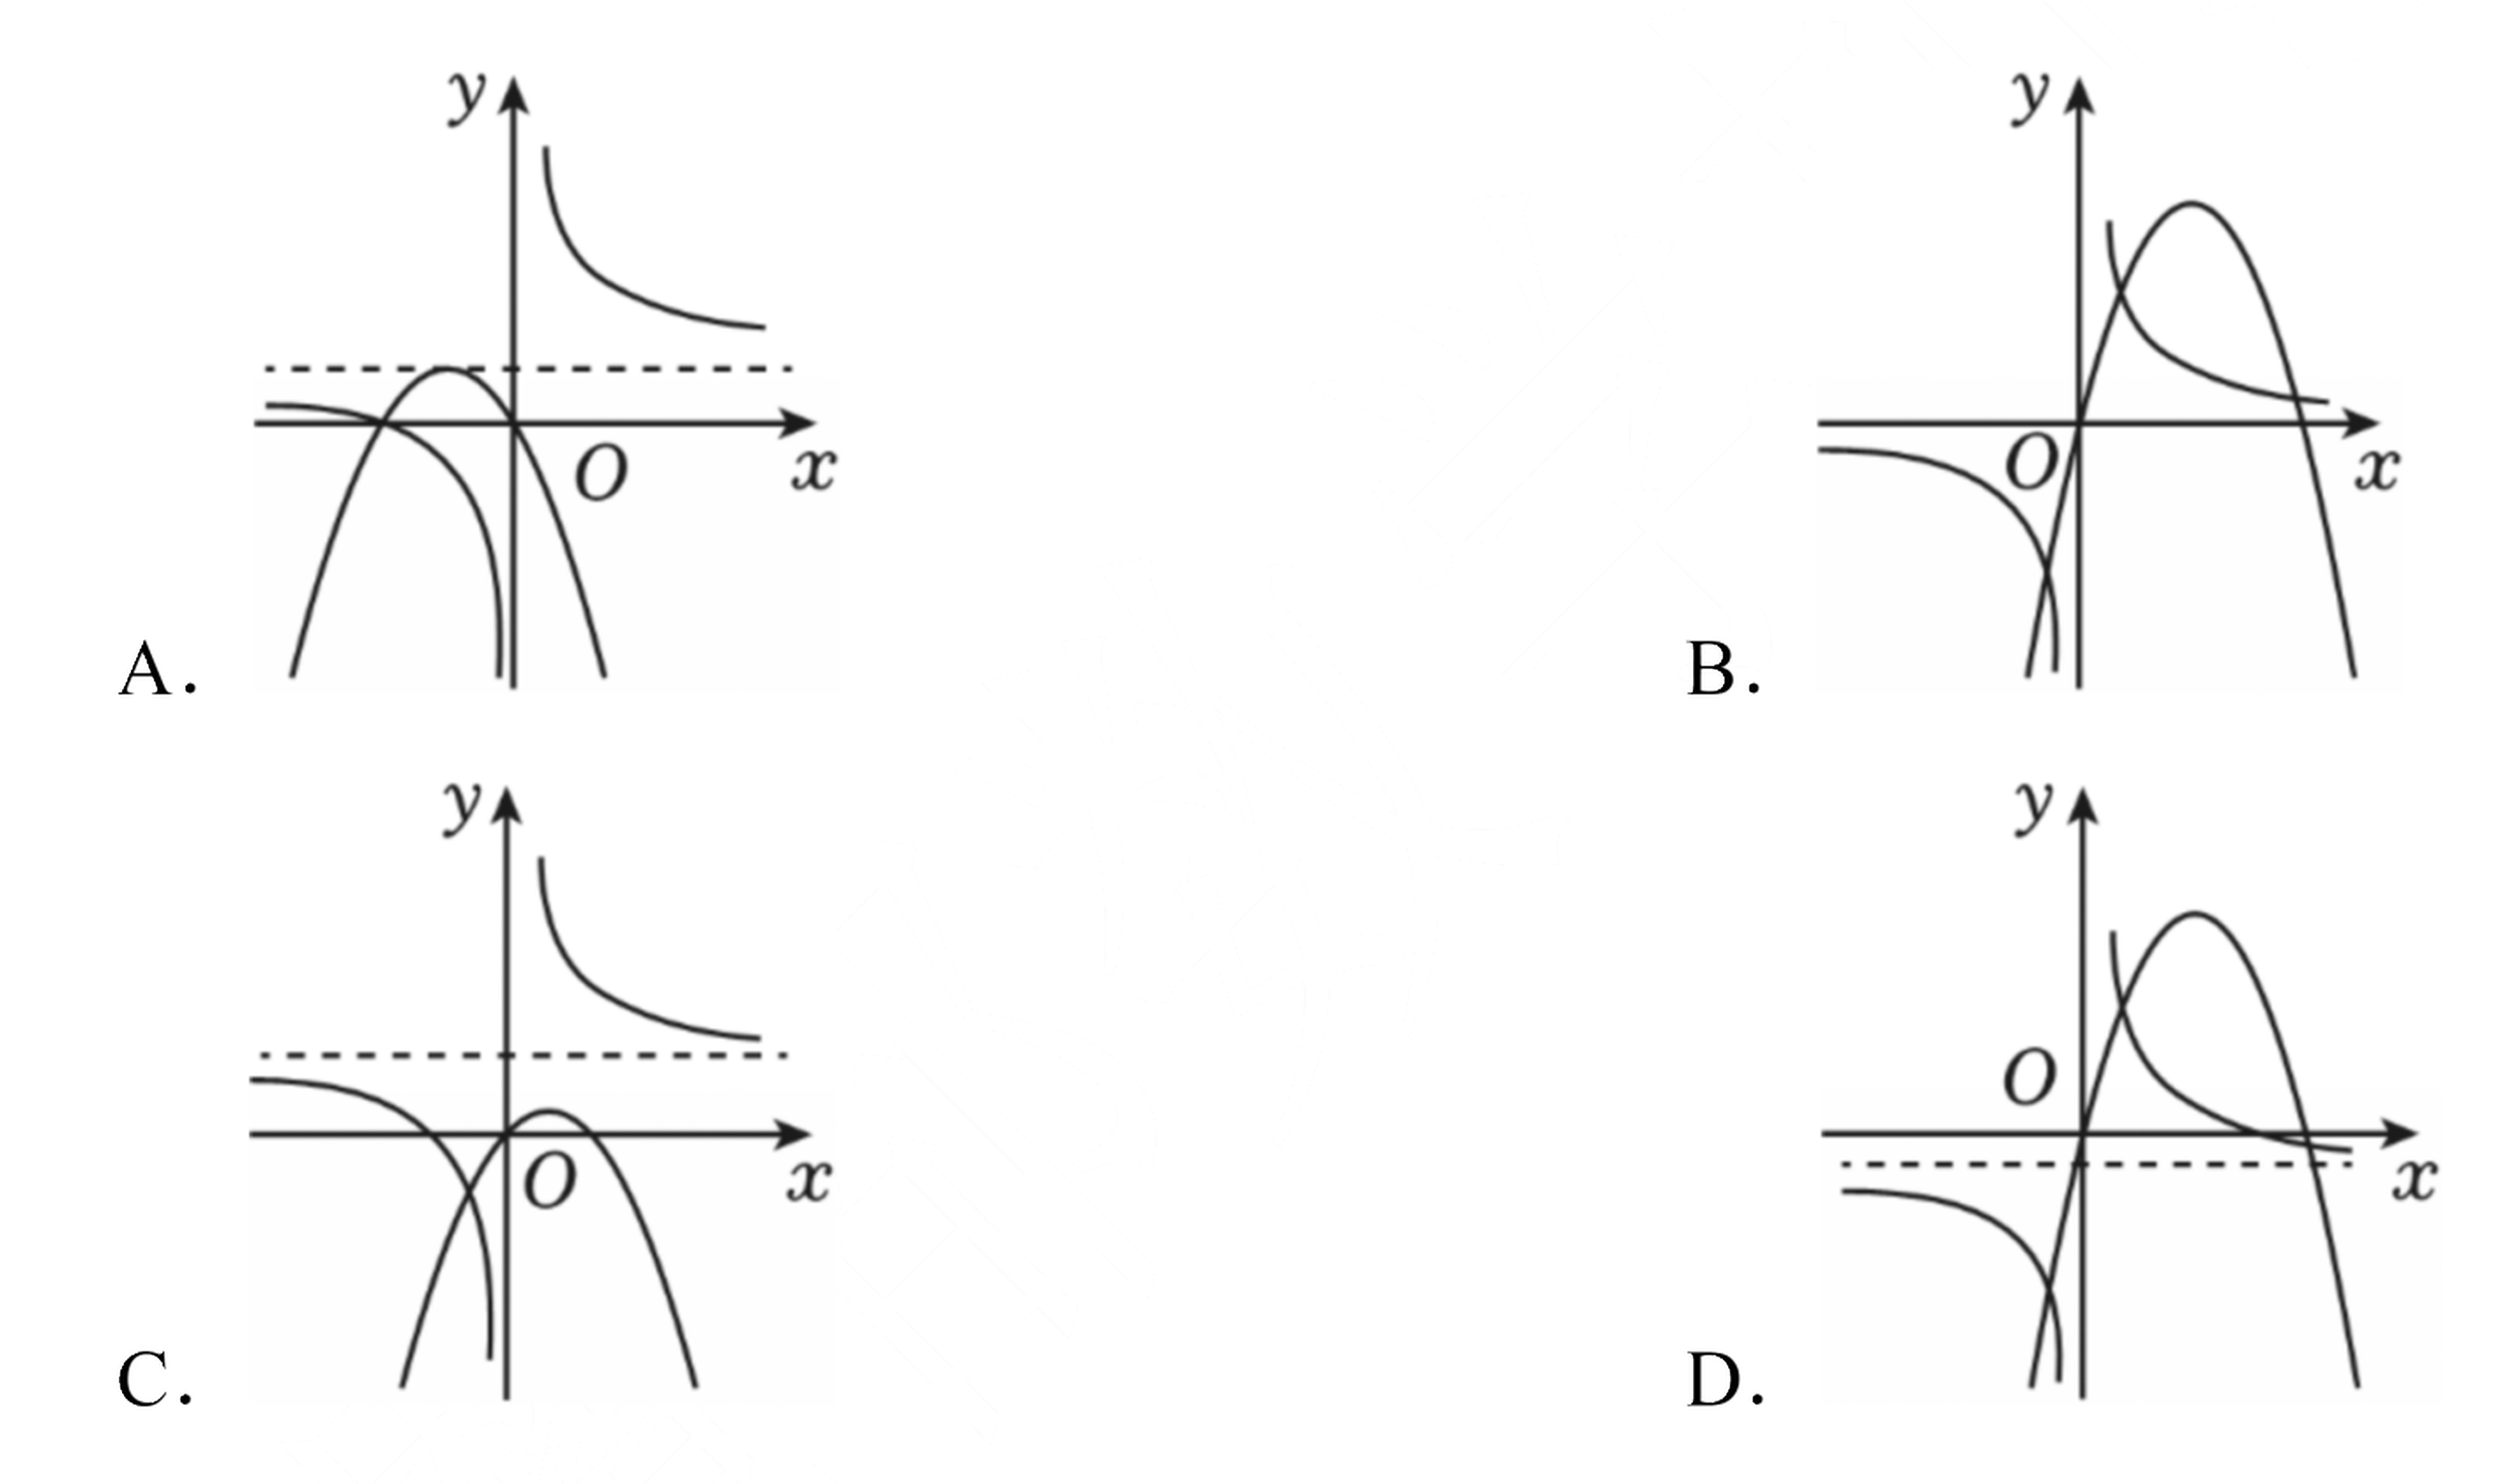
\includegraphics[width=0.80\textwidth]{figures/gao161_q14.png}
\end{center}

\ifanswer
\solbegin
\step{$A$ 选项，由二次函数图象得 $a<0$，$b<0$，由幂函数型函数图象得 $a<0$，$b>0$，}
\step{故 $A$ 选项错误；}
\step{$B$ 选项，由二次函数图象得 $a<0$，$b>0$，由幂函数型函数图象得 $a<0$，$b=0$，}
\step{故 $B$ 选项错误；}
\step{$C$ 选项，由二次函数图象得 $a<0$，$b>0$，由幂函数型函数图象得 $a<0$，$b>0$，}
\step{故 $C$ 选项正确；}
\step{$D$ 选项，由二次函数图象得 $a<0$，$b>0$，由幂函数型函数图象得 $a<0$，$b<0$，}
\step{故 $D$ 选项错误.}
\step{故选 $C$.}
\solend
\fi

% === Q15 === \subseteq／\subset、\varnothing、\mid；"排除 C""排除 B、D"正体字母照录；解析 4 行，故选 $A$
\item 设不等式 $\lvert f(x)\rvert+\lvert g(x)\rvert<a$（常数 $a>0$）的解集是 $M$，设不等式 $\lvert f(x)+g(x)\rvert<a$（常数 $a>0$）的解集是 $N$，则\mbox{（\quad）}

\keepwithprev
A. $M\subseteq N$\qquad B. $N\subseteq M$\qquad C. $M\subset N$\qquad D. $N\subset M$

\ifanswer
\solbegin
\step{$x\in M\Rightarrow\lvert f(x)+g(x)\rvert\leqslant\lvert f(x)\rvert+\lvert g(x)\rvert<a\Rightarrow x\in N$，所以 $M\subseteq N$.}
\step{取 $f(x)=g(x)=0$，则 $M=N$，排除 C.}
\step{取 $f(x)=1$，$g(x)=-1$，$a=1$，则 $M=\varnothing$，$N$ 为全体实数，排除 B、D.}
\step{故选 $A$.}
\solend
\fi

% === Q16 === "人文集"定义证明；cases 无；解析 21 行，故选 $B$
\item 设集合 $I_n=\{1,2,\cdots,n\}$，$n\in\N,n\geqslant1$，集合 $P_n=\left\{\dfrac{m}{\sqrt k}\mid m\in I_n,k\in I_n\right\}$，若 $P_n$ 的子集 $A$ 中任意两个元素之和不是整数的平方，则称 $A$ 为 “人文集”. 那么使 $P_n$ 能分成两个交集为空集的 “人文集” 的并集，且这两个人文集的并集恰为 $P_n$ 时，$n$ 的最大值是\mbox{（\quad）}

\keepwithprev
A. 13\qquad B. 14\qquad C. 15\qquad D. 16

\ifanswer
\solbegin
\step{先证当 $n\geqslant15$ 时，$P_n$ 不能分成两个不相交的人文集的并集.}
\step{假设当 $n\geqslant15$ 时，$P_n$ 可以分成两个不相交的人文集的并集，}
\step{设 $A$ 和 $B$ 为两个不相交的人文集，使 $A\cup B=P_n\supseteq I_n$.}
\step{不妨设 $1\in A$，则由于 $1+3=2^2$，所以 $3\notin A$，即 $3\in B$.}
\step{同理可得，$6\in A$，$10\in B$. 又推出 $15\in A$，}
\step{但 $1+15=4^2$，这与 $A$ 为人文集相矛盾.}
\step{再证 $P_{14}$ 满足要求. 当 $k=1$ 时，$P_{14}=\left\{\dfrac{m}{\sqrt k}\mid m\in I_{14},k\in I_{14}\right\}$，}
\step{可以分成 2 个人文集的并集.}
\step{事实上，只要取 $A_1=\{1,2,4,6,9,11,13\}$，$B_1=\{3,5,7,8,10,12,14\}$，}
\step{则 $A_1$ 和 $B_1$ 都是人文集，且 $A_1\cup B_1=P_{14}$.}
\step{当 $k=4$ 时，集合 $\left\{\dfrac{m}{\sqrt k}\mid m\in I_{14}\right\}$ 中，除整数外，}
\step{剩下的数组成集合 $\left\{\dfrac12,\dfrac32,\dfrac52,\cdots,\dfrac{13}{2}\right\}$，}
\step{可以分为下列 2 个人文集的并：$A_2=\left\{\dfrac12,\dfrac52,\dfrac92,\dfrac{11}{2}\right\}$，$B_2=\left\{\dfrac32,\dfrac72,\dfrac{13}{2}\right\}$.}
\step{当 $k=9$ 时，集合 $\left\{\dfrac{m}{\sqrt k}\mid m\in I_{14}\right\}$ 中，除整数外，}
\step{剩下的数组成集合 $\left\{\dfrac13,\dfrac23,\dfrac43,\dfrac53,\cdots,\dfrac{13}{3},\dfrac{14}{3}\right\}$，}
\step{可以分为下列 2 个人文集的并：$A_3=\left\{\dfrac13,\dfrac43,\dfrac53,\dfrac{10}{3},\dfrac{13}{3}\right\}$，$B_3=\left\{\dfrac23,\dfrac73,\dfrac83,\dfrac{11}{3},\dfrac{14}{3}\right\}$.}
\step{最后，集合 $C=\left\{\dfrac{m}{\sqrt k}\mid m\in I_{14},k\in I_{14},k\ne1,4,9\right\}$ 中的数的分母都是无理数，}
\step{它与 $P_n$ 中的任何其他数之和都不是整数，}
\step{因此，令 $A=A_1\cup A_2\cup A_3\cup C$，$B=B_1\cup B_2\cup B_3$，}
\step{则 $A$ 和 $B$ 是不相交的人文集，且 $A\cup B=P_{14}$.}
\step{综上，$n$ 的最大值为 14，故选 $B$.}
\solend
\fi

\end{enumerate}

\bigsec{三、解答题}

\begin{enumerate}
\setcounter{enumi}{16}

% === Q17 === "图像"照录；\Z；cases 块；解析 9 行，跨 06—07 页
\item (1) 已知函数 $y=x^{\frac{4m-m^2}{2}}$（$m\in\Z$）在区间 $(0,+\infty)$ 上是严格增函数，它的图像关于 $y$ 轴对称，求 $m$ 的值及该函数的解析式；

(2) 若 $(a-2)^{\frac32}<(1+2a)^{\frac32}$，求实数 $a$ 的取值范围.

\ifanswer
\solbegin
\step{(1) 由幂函数在 $(0,+\infty)$ 上严格递增，得 $\dfrac{4m-m^2}{2}>0\Leftrightarrow0<m<4$，}
\step{又 $m\in\Z$，所以 $m\in\{1,2,3\}$.}
\step{当 $m=1$ 或 $m=3$ 时，函数为 $y=x^{\frac32}$，定义域为 $[0,+\infty)$，}
\step{图像不关于 $y$ 轴对称.}
\step{当 $m=2$ 时，函数为 $y=x^2$，满足题意，所以 $m=2$，解析式 $y=x^2$.}
\step{(2) 原不等式有意义，须满足 $\begin{cases}a-2\geqslant0\\1+2a\geqslant0\end{cases}\Leftrightarrow a\geqslant2$，}
\step{函数 $y=x^{\frac32}$ 在 $[0,+\infty)$ 上严格递增，}
\step{因此 $(a-2)^{\frac32}<(1+2a)^{\frac32}\Leftrightarrow a-2<1+2a\Leftrightarrow a>-3$，}
\step{结合 $a\geqslant2$，得 $a\in[2,+\infty)$.}
\solend
\fi

% === Q18 === 题干"$a\geqslant0$"与解析"$a<0$"自相矛盾照录；"$A\cap B=(-2,-1]\cap[2,6)$"误印 ∩ 照录；\subseteq；解析 10 行
\item 已知实数 $a\geqslant0$，集合 $A=\left\{x\mid\dfrac{x+2}{x-6}<0\right\}$，$B=\{x\mid\lvert2x-1\rvert\geqslant3\}$，$C=\{x\mid x^2-3ax+2a^2<0\}$，

(1) 求 $A\cap B$；

(2) 若 $C\subseteq(A\cap B)$，求 $a$ 的取值范围.

\ifanswer
\solbegin
\step{(1) 由 $\dfrac{x+2}{x-6}<0$ 得 $-2<x<6$，即 $A=\{x\mid-2<x<6\}=(-2,6)$，}
\step{由 $\lvert2x-1\rvert\geqslant3$ 得 $2x-1\geqslant3$ 或 $2x-1\leqslant-3$，解得 $x\geqslant2$ 或 $x\leqslant-1$，}
\step{即 $B=(-\infty,-1]\cup[2,+\infty)$，}
\step{所以 $A\cap B=(-2,-1]\cap[2,6)$；}% 原卷把 ∪ 误印成 ∩，照录未改（见 ⑤ 2）
\step{(2) 由 (1) 得 $A\cap B=\{x\mid-2<x\leqslant-1\text{ 或 }2\leqslant x<6\}$，}
\step{因为 $C\subseteq(A\cap B)$，$x^2-3ax+2a^2=(x-a)(x-2a)<0$，}% 题干 $a\geqslant0$ 与解析 $a<0$ 自相矛盾，照录未改（见 ⑤ 1）
\step{当 $a=0$ 时，$C=\varnothing$，符合题意；}
\step{当 $a>0$ 时，$C=(a,2a)$，则 $\begin{cases}a\geqslant2\\2a\leqslant6\\a>0\end{cases}$，解得 $2\leqslant a\leqslant3$，}
\step{当 $a<0$ 时，$C=(2a,a)$，则 $\begin{cases}2a\geqslant-2\\a\leqslant-1\\a<0\end{cases}$，解得 $a=-1$，}
\step{故 $a$ 的范围为 $\{-1,0\}\cup[2,3]$.}
\solend
\fi

% === Q19 === 双碳太阳能应用题；"双碳""自发自用、市电互补"弯引号；解析 8 行，跨 08 页上下
\item 为响应 “双碳” 目标，某电子企业拟安装一套可使用 10 年的太阳能供电设备. 该设备的安装费用 $P(x)$（单位：万元）与太阳能电池板面积 $x(x>0)$（单位：平方米）成正比，比例系数为 $\dfrac12$. 为保障生产用电，安装后采用 “自发自用、市电互补” 模式，在此模式下，企业每年消耗的电费 $Q(x)$（单位：万元）与安装的这种太阳能电池板的面积 $x$ 之间的函数关系是 $Q(x)=\dfrac{180}{x+5}$. 记 $W(x)$（单位：万元）为该企业安装这种太阳能供电设备的费用与 10 年所消耗的电费之和.

(1) 要使该设备的安装费与第 1 年的电费之和不超过 17 万元，求安装太阳能电池板面积 $x$ 的取值范围；

(2) 当 $x$ 为多少平方米时，$W(x)$ 取得最小值？最小值是多少万元？

\ifanswer
\solbegin
\step{(1) $P(x)=\dfrac{x}{2}$，安装费与第 1 年的电费之和不超过 17 万元，即 $\dfrac{x}{2}+\dfrac{180}{x+5}\leqslant17$，}
\step{$x>0$，上式等价于 $x^2-29x+190\leqslant0\Leftrightarrow(x-10)(x-19)\leqslant0$，}
\step{解得 $x\in[10,19]$.}
\step{(2) 安装费用与 10 年电费之和为 $W(x)=P(x)+10Q(x)$，}
\step{$=\dfrac{x}{2}+\dfrac{1800}{x+5}=\dfrac{x+5}{2}+\dfrac{1800}{x+5}-\dfrac52$，}
\step{$x>0$，由基本不等式得 $W(x)\geqslant2\sqrt{\dfrac{x+5}{2}\cdot\dfrac{1800}{x+5}}-\dfrac52=60-\dfrac52=57.5$，}
\step{等号当且仅当 $\dfrac{x+5}{2}=\dfrac{1800}{x+5}$，即 $x=55$ 时成立.}
\step{因此，当电池板面积为 55 平方米时，$W(x)$ 取得最小值 57.5 万元.}
\solend
\fi

% === Q20 === $a*b$ 定义；\min 改正体；cases 块；解析 23 行，跨 08—10 页
\item 设 $a$、$b\in\R$，定义 $a*b=\begin{cases}a,&a<b\\b,&a\geqslant b\end{cases}$.

(1) 若 $x*2>1$，求 $x$ 的取值范围；

(2) 若 $(\lvert x-1\rvert+\lvert x-2\rvert)*3=3$，求 $x$ 的取值范围；

(3) 若 $a$、$b>0$，记 $M=a*\dfrac{b}{a^2+4b^2}$，分别比较 $M$ 与 $a$，以及 $M$ 与 $\dfrac{b}{a^2+4b^2}$ 的大小，并求 $M$ 的最大值.

\ifanswer
\solbegin
\step{(1) 定义 $a*b=\begin{cases}a,&a<b\\b,&a\geqslant b\end{cases}$，由 $x*2>1$，得 $\begin{cases}x<2\\x>1\end{cases}$，或 $\begin{cases}x\geqslant2\\2>1\end{cases}$，}
\step{解得 $x>1$，即 $x$ 的取值范围为 $\{x\mid x>1\}$；}
\step{(2) 当 $x\geqslant2$ 时，$\lvert x-1\rvert+\lvert x-2\rvert=2x-3\geqslant1$，}
\step{当 $1\leqslant2x-3\leqslant3$，即 $2\leqslant x\leqslant3$ 时，}
\step{此时 $(\lvert x-1\rvert+\lvert x-2\rvert)*3=2x-3=3$，解得 $x=3$；}
\step{当 $2x-3>3$，即 $x>3$ 时，}
\step{此时 $(\lvert x-1\rvert+\lvert x-2\rvert)*3=3$ 恒成立，则 $x>3$；}
\step{当 $-2x+3>3$，即 $x<0$ 时，}
\step{此时 $(\lvert x-1\rvert+\lvert x-2\rvert)*3=3$ 恒成立，则 $x<0$.}
\step{当 $1<x<2$ 时，$\lvert x-1\rvert+\lvert x-2\rvert=1$，}
\step{此时 $(\lvert x-1\rvert+\lvert x-2\rvert)*3=1\ne3$，不符合题意；}
\step{当 $x\leqslant1$ 时，$\lvert x-1\rvert+\lvert x-2\rvert=-2x+3\geqslant1$，}
\step{当 $-2x+3\leqslant3$，即 $0\leqslant x\leqslant1$ 时，}
\step{此时 $(\lvert x-1\rvert+\lvert x-2\rvert)*3=-2x+3=3$，解得 $x=0$.}
\step{综上所述，$x$ 的取值范围为 $\{x\mid x\leqslant0\text{ 或 }x\geqslant3\}$；}
\step{(3) 由题意，$M=a*\dfrac{b}{a^2+4b^2}=\min\left\{a,\dfrac{b}{a^2+4b^2}\right\}$，}% 原卷印斜体 min，按全稿惯例改正体 \min（见 ② ⑬）
\step{则 $M\leqslant a$，$M\leqslant\dfrac{b}{a^2+4b^2}$.}
\step{因为 $a$、$b>0$，所以 $\dfrac{b}{a^2+4b^2}\leqslant\dfrac{b}{2\sqrt{a^2\cdot4b^2}}=\dfrac{1}{4a}$，}
\step{当且仅当 $a=2b>0$ 时取等号，}
\step{当 $a\geqslant\dfrac{1}{4a}$，即 $a\geqslant\dfrac12$ 时，$M=a*\dfrac{b}{a^2+4b^2}=\dfrac{b}{a^2+4b^2}\leqslant\dfrac{1}{4a}$，}
\step{则 $a=\dfrac12$，$b=\dfrac14$ 时，$M$ 取得最大值 $\dfrac12$；}
\step{当 $0<a<\dfrac12$ 时，$M=a*\dfrac{b}{a^2+4b^2}=a$，此时 $M<\dfrac12$.}
\step{综上所述，$M$ 的最大值为 $\dfrac12$.}
\solend
\fi

% === Q21 === $A_n$／$B_n$／$S_n$／$T_n$ 新定义；题干第 3 问误标 (2) 照录、解析作 (3)；\prec；解析 25 行，跨 10—11 页
\item 对任意正整数 $n$，记集合 $A_n=\{(a_1,a_2,\cdots,a_n)\mid a_1,a_2,\cdots,a_n$ 均为非负整数，且 $a_1+a_2+\cdots+a_n=n\}$，集合 $B_n=\{(b_1,b_2,\cdots,b_n)\mid b_1,b_2,\cdots,b_n$ 均为非负整数，且 $b_1+b_2+\cdots+b_n=2n\}$. 设 $\alpha=(a_1,a_2,\cdots,a_n)\in A_n$，$\beta=(b_1,b_2,\cdots,b_n)\in B_n$，若对任意 $i\in\{1,2,\cdots,n\}$ 都有 $a_i\leqslant b_i$，则记 $\alpha\prec\beta$.

(1) 写出集合 $A_2$ 和 $B_2$；

(2) 证明：对任意 $\alpha\in A_n$，存在 $\beta\in B_n$，使得 $\alpha\prec\beta$；

(2) 设集合 $S_n=\{(\alpha,\beta)\mid\alpha\in A_n,\beta\in B_n,\alpha\prec\beta\}$，求证：$S_n$ 中的元素个数是完全平方数.% 原卷第 3 问题干误标 (2)（与第 2 问重号），照录未改（见 ⑤ 3）

\ifanswer
\solbegin
\step{(1) $A_2=\{(0,2),(1,1),(2,0)\}$，$B_2=\{(0,4),(1,3),(2,2),(3,1),(4,0)\}$；}
\step{(2) 对任意 $\alpha=(a_1,a_2,\cdots,a_n)\in A_n$，设 $b_i=a_i+1$（$i=1,2,3,\cdots,n$），}
\step{则 $b_1,b_2,\cdots,b_n$ 均为非负整数，且 $a_i\leqslant b_i$（$i=1,2,3,\cdots,n$）.}
\step{令 $\beta=(b_1,b_2,\cdots,b_n)$，则 $b_1+b_2+\cdots+b_n$}
\step{$=(a_1+1)+(a_2+1)+\cdots+(a_n+1)=(a_1+a_2+\cdots+a_n)+n=2n$，}
\step{所以 $\beta\in B_n$，且 $\alpha\prec\beta$.}
\step{(3) 对任意 $\alpha=(a_1,a_2,\cdots,a_n)\in A_n$，$\alpha'=(a_1',a_2',\cdots,a_n')\in A_n$，}
\step{记 $\alpha+\alpha'=(a_1+a_1',a_2+a_2',\cdots,a_n+a_n')$，}
\step{则 $a_1+a_1',a_2+a_2',\cdots,a_n+a_n'$ 均为非负整数，}
\step{且 $(a_1+a_1')+(a_2+a_2')+\cdots+(a_n+a_n')$}
\step{$=(a_1+a_2+\cdots+a_n)+(a_1'+a_2'+\cdots+a_n')=n+n=2n$，}
\step{所以 $\alpha+\alpha'\in B_n$，且 $\alpha\prec\alpha+\alpha'$，$\alpha'\prec\alpha+\alpha'$.}
\step{设集合 $A_n$ 中的元素个数为 $t$，设 $A_n=\{\alpha_1,\alpha_2,\cdots,\alpha_t\}$.}
\step{设集合 $T_n=\{(\alpha_i,\alpha_i+\alpha_j)\mid i=1,2,\cdots,t,j=1,2,\cdots,t\}$.}
\step{对任意 $\alpha_i\in A_n$（$i=1,2,\cdots,t$），都有 $\alpha_i+\alpha_1,\alpha_i+\alpha_2,\cdots,\alpha_i+\alpha_t\in B_n$，}
\step{且 $\alpha_i\prec\alpha_i+\alpha_j$，$j=1,2,\cdots,t$，所以 $T_n\subseteq S_n$.}
\step{若 $(\alpha,\beta)\in S_n$，其中 $\alpha=(a_1,a_2,\cdots,a_n)\in A_n$，$\beta=(b_1,b_2,\cdots,b_n)\in B_n$，}
\step{设 $c_i=b_i-a_i$（$i=1,2,\cdots,n$），因为 $a_i\leqslant b_i$，所以 $c_i=b_i-a_i\geqslant0$，}
\step{记 $\alpha'=(c_1,c_2,\cdots,c_n)$，}
\step{则 $c_1+c_2+\cdots+c_n=(b_1-a_1)+(b_2-a_2)+\cdots+(b_n-a_n)$}
\step{$=(b_1+b_2+\cdots+b_n)-(a_1+a_2+\cdots+a_n)=2n-n=n$，}
\step{所以 $\alpha'\in A_n$，并且有 $\beta=\alpha+\alpha'$，所以 $(\alpha,\beta)\in T_n$，所以 $S_n\subseteq T_n$，}
\step{所以 $S_n=T_n$.}
\step{因为集合 $T_n$ 中的元素个数为 $t^2$，所以 $S_n$ 中的元素个数为 $t^2$，}
\step{是完全平方数.}
\solend
\fi

\end{enumerate}

\end{document}
"
% 紧凑版：xelatex "\def\iscompact{1}% 高一161_松江一中嘉一实验_期中.tex
%   —— 高一上数学"2026-2027 年松江一中嘉一实验高一上期中"（试卷版/答案版/紧凑版）
% 试卷版：xelatex 高一161_松江一中嘉一实验_期中.tex
% 答案版：xelatex "\def\isanswer{1}\input{高一161_松江一中嘉一实验_期中.tex}"
% 紧凑版：xelatex "\def\iscompact{1}\input{高一161_松江一中嘉一实验_期中.tex}"
%
% ① 原始材料：微信公众号"魔都数学加油站"文章，连载"27学年高一161"，原卷卷面标题
% "2026-2027 年松江一中嘉一实验高一上期中"（卷面未印副标题、未印连载号）。
% 正文为 11 张 PNG 页（01/02/03/05/06/07/08/09/11 为 4762×6735，04/10 为
% 2560×3620，同一篇各页分辨率混排，逐页按各自分辨率裁图核对）。
% 体例：讲评版——填空 3—12（10 题）、选择 13—16（4 题）、解答 17—21（5 题），
% 共 19 题，自第 3 题起编（1、2 未印在本篇）；Q13 答案"A"直接印在题干括号内、
% 且无【答案】/【解析】段，本稿按 高一37 第 13 题／高一57 第 13 题成例把括号
% 留空、另提 \ans{$A$}；其余 18 题逐题印【解析】、用 \solbegin…\solend。
% 题目、答案、解析均据原图转录；卷面粉红色水印"魔都数学加油站"及公众号页脚未录入。
% 全卷插图清单（逐页通读 11 页确认）：仅 1 组——Q14 四幅图像选项（04 页 2×2
% 排布，二次函数与幂函数型函数在同一坐标系中的图象，A/B/C/D 四幅小图），
% 合并成一张，三版都出，裁 figures/gao161_q14.png。其余各页逐页确认无其它
% 题目配图、无解析内配图、无表格、无"如图"处（Q16 解析里的"可以分为下列 2 个
% 人文集的并"是纯文字＋集合，不是表格；OCR 里看似表格的行实为大括号与分数）。
%
% 卷首标题：原卷印作"2026-2027 年松江一中嘉一实验高一上期中"，年份区间按全稿惯例排 en dash；
% 原卷卷面未印副标题，本稿按同期中卷知识模块口径补出"集合与常用逻辑用语、不等式、函数"。
%
% ② 与原卷的排版差异／照录项清单：
%   ① 原文从第 3 题起，本稿保留原题号；共 19 题三节，解答题 5 题到 21；
%      三节各自一个 enumerate + \setcounter{enumi}{2}/{12}/{16}（不贯穿），
%      用 \examtitlest[3] 起手；
%   ② 混合体例：Q13 原卷把答案"A"直接印在题干括号内（"（  A  ）"）、且题下
%      无【答案】/【解析】段，按 高一37 第 13 题／高一57 第 13 题成例把括号
%      留空、另提 \ans{$A$}、不补造解析；其余 18 题印【解析】、用
%      \solbegin…\solend；四道选择题中 Q14/Q15/Q16 的答案在解析末句
%      "故选 $C$／$A$／$B$"、Q13 用 \ans{$A$}；括号 \mbox{（\quad）} 留空；
%      答案版【答案】/【解析】标记数 = 19 = 全卷题数（1 个 \ans ＋ 18 个 \solbegin）；
%   ③ 原卷卷面未印副标题，本稿按知识模块口径补出；
%   ④ 原卷填空横线按全稿惯例排 \blankline[4.4em]；选择题选项段前按惯例各加
%      \keepwithprev；Q14 四幅选项图整块用 \needvspace{9cm} 守卫（守卫放
%      \item 之前，见 高一132 Q14／高一154 Q15 成例）；解答题不留作答区、
%      不加 \anspace（原卷为讲评版）；
%   ⑤ 数集归一：Q8"$x\in\R$"、Q11"$m\in\R$"、Q13"$x,y\in\N$"、
%      Q16"$n\in N$"、Q17"$m\in\Z$"、Q20"$a$、$b\in R$"——原卷印正体粗体
%      或斜体 R/N/Z，按全稿惯例归一 \R／\N／\Z；绝对值排 \lvert…\rvert
%      （Q9、Q12、Q15、Q18、Q20），集合描述竖线排 \mid（Q12、Q16、Q18、
%      Q20、Q21），空集 \varnothing（Q15、Q18），补集无用例，不等号按全稿
%      惯例排 \leqslant／\geqslant；
%   ⑥ 子集符号逐处照录不统一：Q12 cases 定义"$C(A)\geqslant C(B)$"、
%      Q15 选项 A/B"$M\subseteq N$""$N\subseteq M$"与解析"$M\subseteq N$"
%      印带下划线 ⊆（照录 \subseteq），Q15 选项 C/D"$M\subset N$""$N\subset M$"
%      印单线 ⊂（照录 \subset），Q18 "$C\subseteq(A\cap B)$"、Q21
%      "$T_n\subseteq S_n$""$S_n\subseteq T_n$"均带下划线照录 \subseteq；
%      本卷无 \not\subset 用例；
%   ⑦ 判别式：Q7 解析"$\Delta=(m-6)(m+2)>0$"、Q8 解析"$\Delta=a^2-4a<0$"、
%      Q12 解析"$\Delta=a^2-8$"共 3 处，逐处放大确认印等腰偏高粗三角
%      （高>宽、右斜边粗），照录 \Delta；本卷无扁等边细线 \triangle 用例；
%   ⑧ 中文弯引号照录：Q7"$m\geqslant6$""有两个不相等的正实数根"及四个
%      条件短语、Q13 反证法命题、Q16"人文集"、Q19"双碳""自发自用、市电互补"；
%      注释里一律 ASCII 引号；数学式内 CJK 用 \text{}（Q18、Q20 解集描述内"或"）；
%   ⑨ "图像／图象"逐处照录不统一：Q4"的图像"、Q17 题干"它的图像关于 $y$ 轴
%      对称"及解析"图像不关于 $y$ 轴对称"印"图像"；Q14 题干"的图象可能为"
%      与解析 A/B/C/D 四行各"由二次函数图象得""由幂函数型函数图象得"
%      共 8 处印"图象"（象，无亻）；
%   ⑩ 文本圈数字逐处照录：Q12 题干①②③④、Q12 解析"故①错误""故②正确"
%      "故③正确""故④错误""故正确的是②③"，均为印刷圈数字（文本模式）；
%   ⑪ 半角逗号在数学组之间是全稿惯例、非笔误，逐处照录（Q5"$a$、$b$"、
%      Q13"$x,y\in\N$"、Q16"$n\in\N,n\geqslant1$"与集合描述内逗号、
%      Q20"$a,b\in\R$"、Q21 各集合描述内逗号）；行末西文句点 ASCII `.`；
%      原卷行中句点（Q16"$10\in B$. 又推出 $15\in A$"、Q16"再证 $P_{14}$
%      满足要求. 当 $k=1$ 时"、Q18"$A\cap B=(-2,-1]\cap[2,6)$；"后的分号）
%      按全稿惯例一律排 ASCII `.`／全角"；"；中文语境行中全角逗号／顿号照录；
%   ⑫ 原卷数学式内联条件（Q14"$y=x^a+b(a\ne0)$"、Q19"$x(x>0)$"、
%      Q11"$\lvert x-m\rvert<n\,(m\in\R,n>0)$"）印半角括号，逐处照录未改
%      全角（同 高一147 口径）；
%      中文语境的括注（Q5"结果用 $a$、$b$ 表示"、Q7"填…"、Q12"填写序号"、
%      Q15"常数 $a>0$"、Q19"单位：万元"）印全角括号，照录；
%   ⑬ 复杂式照录别简化：Q3 $(a^{2-\sqrt3})^{2+\sqrt3}\times\sqrt{a^2}\times
%      b^{\sqrt3}\times b^{1-\sqrt3}$ 与 $a^{(2-\sqrt3)(2+\sqrt3)}\cdot a\cdot
%      b^{\sqrt3+1-\sqrt3}=a\cdot a\cdot b=a^2b$（题干用 \times、解析用 \cdot，
%      逐处照录不统一，见 ⑤）；Q5 $\dfrac{\lg2}{\lg2+\lg3}=\dfrac{a}{a+b}$、
%      Q10 $t-\dfrac3t=2$ 与 $b=a^3$、$ab=a^4=2$、Q11 $\left(2a-\dfrac12
%      -a+\dfrac12,2a-\dfrac12+a-\dfrac12\right)=(a,3a-1)$ 与
%      $\left(\dfrac43,\dfrac53\right]\cup\{2\}$、Q16 各分数集合、Q19
%      $x^2-29x+190\leqslant0$ 与 $W(x)=P(x)+10Q(x)$ 与
%      $2\sqrt{\dfrac{x+5}{2}\cdot\dfrac{1800}{x+5}}-\dfrac52=60-\dfrac52=57.5$、
%      Q20 $M=a*\dfrac{b}{a^2+4b^2}=\min\left\{a,\dfrac{b}{a^2+4b^2}\right\}$
%      与 $\dfrac{b}{2\sqrt{a^2\cdot4b^2}}=\dfrac{1}{4a}$、Q21 各 $A_n$／$B_n$／
%      $T_n$ 定义；\left…\right 不得拆到不同 $…$ 组（Q11 的 \left(…\right)、
%      Q11 的 \left(\dfrac43,\dfrac53\right]、Q16 的 \left\{\dfrac{m}{\sqrt k}
%      \mid…\right\} 与 \left\{\dfrac12,\dfrac32,\dfrac52,\cdots,\dfrac{13}{2}\right\}
%      等、Q20 的 \min\left\{…\right\}）；cases 块整体算一个印刷行
%      （Q12 定义、Q17 (2)、Q18 (2) 两处、Q20 定义与 (1)）；原卷 Q20 解析
%      "$=min\{…\}$"印斜体 min，按 高一122／高一102 成例改正体 \min；
%   ⑭ 一条 \step = 原卷解析的一个印刷行；别并折行、别拆行。跨页续印按题合并
%      （Q6 的 01 页上下题干重复印、Q10 的 01—02 页、Q11 的 02—03 页、
%      Q12 的 03—04 页、Q16 的 05—06 页、Q17 的 06—07 页、Q18 的 07 页
%      上下、Q19 的 08 页上下、Q20 的 08—10 页、Q21 的 10—11 页）；
%      跨半页重叠行（Q10"令 $t=\log_a b>0$…"、Q16"它与 $P_n$ 中的任何
%      其他数之和都不是整数，"、Q18"【解析】(1) 由 $\dfrac{x+2}{x-6}<0$…"、
%      Q19"$x>0$，上式等价于…"、Q20"此时…则 $x<0$."、Q21"若 $(\alpha,\beta)
%      \in S_n$…"与"设 $c_i=b_i-a_i$…"）只算一个印刷行；
%   ⑮ 自定义记号照录：Q12"$C(A)$""$A*B$""$S$"、Q16"$I_n$""$P_n$""人文集"
%      "$A_1$／$B_1$／$A_2$／$B_2$／$A_3$／$B_3$／$C$"、Q20"$a*b$""$M$"、
%      Q21"$A_n$／$B_n$／$S_n$／$T_n$""$\alpha\prec\beta$""$\alpha+\alpha'$"；
%   ⑯ 选项字母体例照录不统一：Q15 解析"排除 C.""排除 B、D."两处原卷印
%      正体（文本模式），Q13 \ans{$A$}、Q14"$A$ 选项"…"故选 $C$"、
%      Q15"故选 $A$"、Q16"故选 $B$"用斜体（数学模式），逐处照录、不统一；
%   ⑰ 红字：全卷逐页扫描无红色加粗小标题（仅粉色水印），故本卷无 \stepm，
%      不引入红色定义；
%
% ③ 行数复核：一条 \step = 原卷解析的一个印刷行，cases 块作一个印刷行计。
%   逐题数（逐页核对定稿）：Q3：1；Q4：1；Q5：1；Q6：3；Q7：4；Q8：4；
%   Q9：2；Q10：2；Q11：7；Q12：8；Q13：0（答案印括号内、提 \ans{}，
%   不计入 \step 账）；Q14：9；Q15：4；Q16：21；Q17：9；Q18：10；Q19：8；
%   Q20：23；Q21：25。
%   合计 142 行（142 条 \step，无 \stepm），与原卷逐题印刷行相等。
%   全卷 19 题：Q13 一处 \ans{} ＋ 其余 18 题设 \solbegin…\solend，
%   答案版【答案】/【解析】标记数 = 19 = 全卷题数。
%
% ④ 页码分布（供回原图复核）：
%   卷首标题＋"一、填空题"＋Q3/Q4/Q5 题干＋解析各 1 行＋Q6 题干首行
%   在 01 页上半；Q6 题干（重复印）＋解析 3 行＋Q7 题干＋解析 4 行在
%   01 页下半；Q8 题干＋解析 4 行＋Q9 题干＋解析 2 行＋Q10 题干＋
%   解析首行在 02 页上半；Q10 解析（重复印）＋末行＋Q11 题干＋解析
%   前 3 行在 02 页下半；Q11 解析后 4 行＋Q12 题干＋cases 定义＋①
%   在 03 页上半；Q12 ②③④ 三命题＋"填写序号"行＋解析前 6 行在
%   03 页下半；Q12 解析后 2 行＋"二、选择题"标题＋Q13 题干＋选项＋
%   Q14 题干＋"（　）"＋A/B 两幅图在 04 页上半；Q14 四幅图（重复印）
%   ＋解析 9 行在 04 页下半；Q15 题干＋选项＋解析 4 行＋Q16 题干＋
%   选项在 05 页上半；Q16 题干（重复印）＋选项＋解析前 10 行在 05 页
%   下半；Q16 解析中 8 行（k=4、k=9 两批＋集合 C＋"它与 $P_n$…"）
%   在 06 页上半；Q16 解析"它与 $P_n$…"（重复印）＋末 3 行＋
%   "三、解答题"标题＋Q17 题干＋两问＋解析前 4 行在 06 页下半；
%   Q17 解析后 5 行＋Q18 题干＋两问＋解析首行在 07 页上半；Q18 解析
%   （重复首行）＋余 9 行在 07 页下半；Q19 题干＋两问＋解析前 2 行在
%   08 页上半；Q19 解析（重复第 2 行）＋余 6 行＋Q20 定义＋(1) 问在
%   08 页下半；Q20 (2)(3) 两问＋解析 (1) 2 行＋(2) 前 7 行在 09 页
%   上半；Q20 解析 (2) 余 4 行＋(3) 前 4 行在 09 页下半；Q20 解析 (3)
%   余 4 行＋Q21 题干＋三问在 10 页上半；Q21 题干（重复印）＋解析
%   (1)(2)(3) 前 8 行在 10 页下半；Q21 解析 (3) 中 10 行在 11 页上半；
%   Q21 解析 (3)（重复 2 行）＋末 7 行"是完全平方数."在 11 页下半。
%   本稿按题连排，不丢行、不并折行；全卷末题为第 21 题，无附加题节。
%
% ⑤ 存疑照录（放大原图确认，照录未改、正文对应处另有 % 注）：
%   1. Q18 题干印"已知实数 $a\geqslant0$"，解析却另设"当 $a<0$ 时"并解出
%      $a=-1$，末行答案"故 $a$ 的范围为 $\{-1,0\}\cup[2,3]$"含负数，
%      与题干 $a\geqslant0$ 自相矛盾——系原卷前后不一，照录未改（放大
%      07 页确认题干确印 $a\geqslant0$）；
%   2. Q18 解析"所以 $A\cap B=(-2,-1]\cap[2,6)$；"原卷把并集误印成
%      交集号 ∩（紧接下一行"$A\cap B=\{x\mid-2<x\leqslant-1$ 或
%      $2\leqslant x<6\}$"用"或"），照录未改（放大 07 页确认印 ∩）；
%   3. Q21 题干第 3 问原卷标号印作"(2)"（与第 2 问重号），而解析里
%      同一问标作"(3)"——原卷笔误，题干与解析逐处照录、不统一；
%   4. Q3 题干四处乘号印"×"（\times）、解析内三处乘号印"·"（\cdot），
%      逐处照录未统一（放大 01 页确认）；
%   5. Q16 解析"先证当 $n\geqslant15$ 时"印 ≥（非 >），与"综上，$n$
%      的最大值为 14"自洽，照录；题干"$n\in N,n\geqslant1$"印斜体
%      $N$、按全稿惯例归一 \N（见 ② ⑤）；
%   6. Q20 解析"$M=a*\dfrac{b}{a^2+4b^2}=min\{…\}$"原卷印斜体 min，
%      按全稿惯例改正体 \min（见 ② ⑬）；末行"$M$ 的最大值为
%      $\dfrac12$"照录；
%   7. Q15 解析"排除 C.""排除 B、D."用正体字母，而"故选 $A$"用斜体
%      字母，原卷体例不一（见 ② ⑯），照录未统一。
%   全卷除此 7 类外未发现其它笔误／自相矛盾处；Q13 只把答案印在括号内、
%   其余 18 题全部印【解析】。
%

\documentclass[a4paper,11pt]{article}
\usepackage{common}

\begin{document}

\examtitlest[3]{2026--2027 年松江一中嘉一实验高一上期中}{集合与常用逻辑用语、不等式、函数}

\bigsec{一、填空题}

\begin{enumerate}
\setcounter{enumi}{2}

% === Q3 === 题干 \times、解析 \cdot 逐处照录；解析 1 行
\item 设 $a>0$，$b>0$，化简 $(a^{2-\sqrt3})^{2+\sqrt3}\times\sqrt{a^2}\times b^{\sqrt3}\times b^{1-\sqrt3}=$\blankline[4.4em].

\ifanswer
\solbegin
\step{因为 $a>0$，所以 $\sqrt{a^2}=a$，原式 $=a^{(2-\sqrt3)(2+\sqrt3)}\cdot a\cdot b^{\sqrt3+1-\sqrt3}=a\cdot a\cdot b=a^2b$.}
\solend
\fi

% === Q4 === "图像"照录；解析 1 行
\item 若幂函数 $y=x^a$ 的图像经过点 $(5,\sqrt5)$，则此幂函数的表达式为 $y=$\blankline[4.4em].

\ifanswer
\solbegin
\step{$5^a=\sqrt5\Rightarrow a=\dfrac12$，所以 $y=\sqrt x$.}
\solend
\fi

% === Q5 === "结果用 $a$、$b$ 表示"全角括号＋顿号照录；解析 1 行
\item 已知 $\lg2=a$，$10^b=3$，则 $\log_6 2=$\blankline[4.4em]（结果用 $a$、$b$ 表示）.

\ifanswer
\solbegin
\step{$\lg3=b$，$\log_6 2=\dfrac{\lg2}{\lg2+\lg3}=\dfrac{a}{a+b}$.}
\solend
\fi

% === Q6 === 对称中心；解析 3 行，题干跨 01 页上下重复印
\item 若函数 $y=\dfrac{mx-1}{x+n}$ 的对称中心是 $(4,-3)$，则 $m+n=$\blankline[4.4em].

\ifanswer
\solbegin
\step{令 $x=-n+t$（$t\ne0$），则 $y-m=-\dfrac{mn+1}{t}$；}
\step{将 $t$ 换成 $-t$，$y-m$ 变为其相反数，因此对称中心为 $(-n,m)$.}
\step{于是 $n=-4$，$m=-3$，得 $m+n=-7$.}
\solend
\fi

% === Q7 === 充要条件；中文弯引号＋圈选条件；\Delta 高瘦；解析 4 行
\item 已知关于 $x$ 的一元二次方程 $x^2-mx+m+3=0$，则 “$m\geqslant6$” 是该方程 “有两个不相等的正实数根” 的\blankline[4.4em]条件（填 “充分不必要”、“必要不充分”、“充要” 或 “既不充分也不必要”）.

\ifanswer
\solbegin
\step{方程有两个不相等的正实数根}
\step{$\Leftrightarrow m>0$、$m+3>0$ 且 $\Delta=(m-6)(m+2)>0\Leftrightarrow m>6$.}
\step{$m>6\Rightarrow m\geqslant6$，但 $m=6$ 时方程有两个相等的正实数根，}
\step{因此为必要不充分条件.}
\solend
\fi

% === Q8 === \R、\Delta；解析 4 行
\item 对于任意的 $x\in\R$，代数式 $\lg(ax^2+ax+1)$ 都有意义，则实数 $a$ 的取值范围是\blankline[4.4em].

\ifanswer
\solbegin
\step{真数须满足 $ax^2+ax+1>0$ 对任意 $x\in\R$ 恒成立.}
\step{$a=0$ 时成立；}
\step{$a\ne0$ 时，恒成立等价于 $a>0$ 且 $\Delta=a^2-4a<0$，解得 $0<a<4$；}
\step{因此 $a\in[0,4)$.}
\solend
\fi

% === Q9 === 绝对值 \lvert…\rvert；解析 2 行
\item 若不等式 $\lvert x+1\rvert-\lvert x-4\rvert<m$ 的解集为非空集合，则实数 $m$ 的取值范围是\blankline[4.4em].

\ifanswer
\solbegin
\step{$\lvert x+1\rvert-\lvert x-4\rvert\geqslant-\lvert(x+1)-(x-4)\rvert=-5$，当 $x=-1$ 时取等号，}
\step{因此原不等式的解集非空 $\Leftrightarrow m>-5$，所求范围为 $(-5,+\infty)$.}
\solend
\fi

% === Q10 === 换底；$\log_2 a\cdot\log_2 b$；解析 2 行，跨 02 页上下
\item 已知 $a>1$，$b>1$，若 $\log_a b-3\log_b a=2$，且 $ab=2$，则 $\log_2 a\cdot\log_2 b=$\blankline[4.4em].

\ifanswer
\solbegin
\step{令 $t=\log_a b>0$，则 $t-\dfrac{3}{t}=2\Leftrightarrow(t-3)(t+1)=0$，得 $t=3$，}
\step{于是 $b=a^3$，$ab=a^4=2$，得 $\log_2 a=\dfrac14$，$\log_2 b=\dfrac34$，所求为 $\dfrac{3}{16}$.}
\solend
\fi

% === Q11 === 邻域定义；\left(…\right) 不拆组；解析 7 行，跨 02—03 页
\item 对于实数 $m$ 和正数 $n$，称满足不等式 $\lvert x-m\rvert<n\,(m\in\R,n>0)$ 的实数 $x$ 的集合叫做 $m$ 的 $n$ 邻域. 已知 $a>\dfrac12$，若 $2a-\dfrac12$ 的 $a-\dfrac12$ 邻域中恰有 2 个整数，则 $a$ 的取值范围是\blankline[4.4em].

\ifanswer
\solbegin
\step{所求邻域为 $\left(2a-\dfrac12-a+\dfrac12,2a-\dfrac12+a-\dfrac12\right)=(a,3a-1)$.}
\step{当 $\dfrac12<a\leqslant1$ 时至多含 1 个整数；}
\step{当 $a>2$ 时，区间长度 $2a-1>3$，至少含 3 个整数.}
\step{当 $1<a<2$ 时，区间必含 2，恰有两个整数等价于 $3<3a-1\leqslant4$，}
\step{即 $\dfrac43<a\leqslant\dfrac53$.}
\step{当 $a=2$ 时，区间为 $(2,5)$，恰含整数 $3,4$；}
\step{所以 $a\in\left(\dfrac43,\dfrac53\right]\cup\{2\}$.}
\solend
\fi

% === Q12 === $C(A)$／$A*B$ 定义题；①②③④ 文本圈数字；\subseteq／\subset、\Delta、\mid、\varnothing；解析 8 行
\item 用 $C(A)$ 表示非空集合 $A$ 中的元素个数. 对于集合 $A$、$B$，定义

$A*B=\begin{cases}C(A)-C(B),&C(A)\geqslant C(B)\\ C(B)-C(A),&C(A)<C(B)\end{cases}$，若 $A=\{0,1\}$，$B=\{x\mid(x^2-ax)(x^2+ax+2)=0\}$，设实数 $a$ 的所有可能取值组成的集合是 $S$，则下列说法正确的是\blankline[4.4em]（填写序号）.

① $C(B)$ 的可能值为 $2,3,4$

② 若 $A*B=2$，则 $a$ 的取值范围为 $(-\infty,-2\sqrt2)\cup(2\sqrt2,+\infty)$

③ 若 $A*B=1$，则 $C(S)=3$

④ 若 $A*B=0$，则 $a$ 的取值范围为 $(-2\sqrt2,2\sqrt2)$

\ifanswer
\solbegin
\step{$x(x-a)=0$ 的根为 $0,a$，而 $x^2+ax+2$ 在这两处的值分别为 $2,2a^2+2$，}
\step{两个因式无公共实根；后者的判别式为 $\Delta=a^2-8$.}
\step{当 $a=0$、$0<\lvert a\rvert<2\sqrt2$、$\lvert a\rvert=2\sqrt2$、$\lvert a\rvert>2\sqrt2$ 时，$C(B)$ 依次为 $1,2,3,4$，}
\step{故①错误.}
\step{$A*B=\lvert2-C(B)\rvert$，所以 $A*B=2\Leftrightarrow\lvert a\rvert>2\sqrt2$，故②正确；}
\step{$A*B=1\Leftrightarrow a\in\{-2\sqrt2,0,2\sqrt2\}$，此时 $C(S)=3$，故③正确；}
\step{$A*B=0\Leftrightarrow0<\lvert a\rvert<2\sqrt2$，即 $a\in(-2\sqrt2,0)\cup(0,2\sqrt2)$，故④错误.}
\step{故正确的是②③.}
\solend
\fi

\end{enumerate}

\needvspace{7cm}
\bigsec{二、选择题}

\begin{enumerate}
\setcounter{enumi}{12}

% === Q13 === 答案"A"原卷印在题干括号内、题下无【答案】/【解析】段；按 高一37／高一57 成例另提 \ans{}
\item 用反证法证明命题 “已知 $x>0$，$y>0$，$x,y\in\N$，如果 $xy$ 可被 7 整除，那么 $x$，$y$ 至少有一个能被 7 整除” 时，假设的内容是\mbox{（\quad）}

\keepwithprev
A. $x$、$y$ 都不能被 7 整除\qquad B. $x$、$y$ 都能被 7 整除

C. $x$、$y$ 只有一个能被 7 整除\qquad D. 只有 $x$ 不能被 7 整除

\ifanswer
\ans{$A$}
\fi

% === Q14 === 四幅图像选项（2×2 合并，三版都出）；守卫放 \item 之前；"图象"照录；解析 9 行，故选 $C$
\needvspace{9cm}
\item 函数 $y=ax^2+bx$ 与函数 $y=x^a+b(a\ne0)$ 在同一平面直角坐标系中的图象可能为\mbox{（\quad）}

\keepwithprev
\begin{center}
% 四幅图象选项取 04 页 2×2 排布合并为一张，去粉色水印、转灰度、4× LANCZOS 放大；三版都出
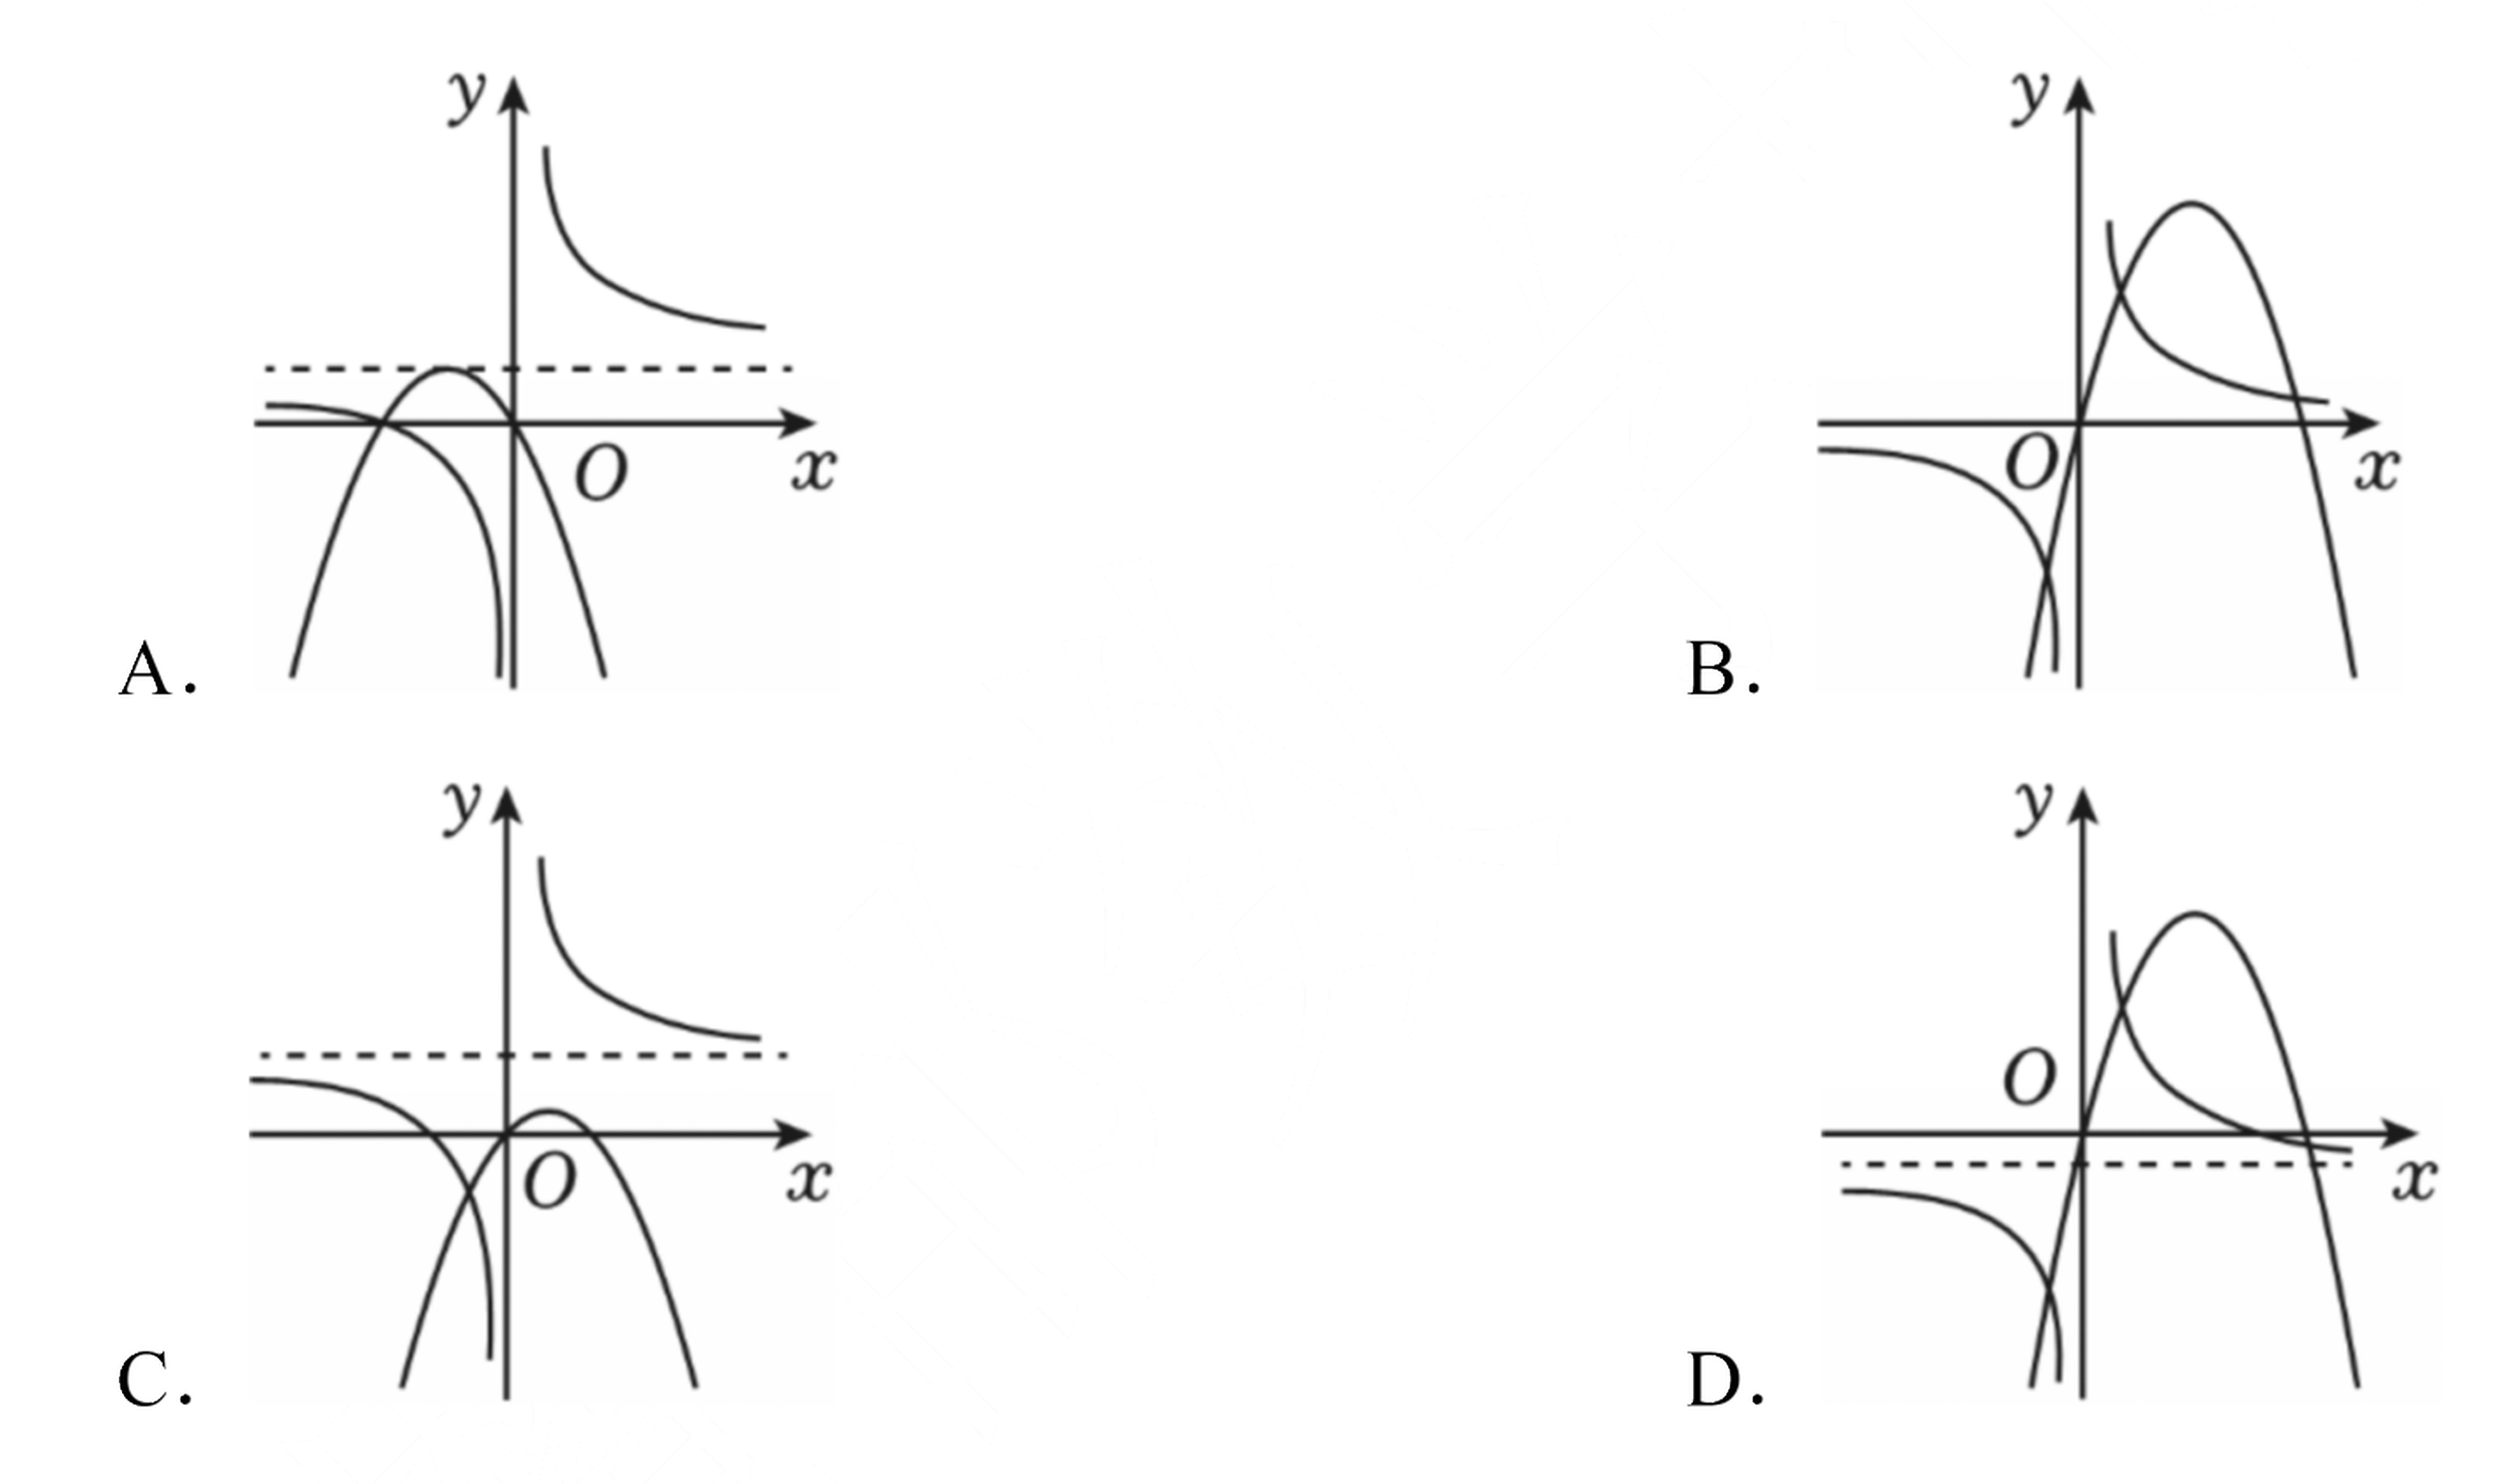
\includegraphics[width=0.80\textwidth]{figures/gao161_q14.png}
\end{center}

\ifanswer
\solbegin
\step{$A$ 选项，由二次函数图象得 $a<0$，$b<0$，由幂函数型函数图象得 $a<0$，$b>0$，}
\step{故 $A$ 选项错误；}
\step{$B$ 选项，由二次函数图象得 $a<0$，$b>0$，由幂函数型函数图象得 $a<0$，$b=0$，}
\step{故 $B$ 选项错误；}
\step{$C$ 选项，由二次函数图象得 $a<0$，$b>0$，由幂函数型函数图象得 $a<0$，$b>0$，}
\step{故 $C$ 选项正确；}
\step{$D$ 选项，由二次函数图象得 $a<0$，$b>0$，由幂函数型函数图象得 $a<0$，$b<0$，}
\step{故 $D$ 选项错误.}
\step{故选 $C$.}
\solend
\fi

% === Q15 === \subseteq／\subset、\varnothing、\mid；"排除 C""排除 B、D"正体字母照录；解析 4 行，故选 $A$
\item 设不等式 $\lvert f(x)\rvert+\lvert g(x)\rvert<a$（常数 $a>0$）的解集是 $M$，设不等式 $\lvert f(x)+g(x)\rvert<a$（常数 $a>0$）的解集是 $N$，则\mbox{（\quad）}

\keepwithprev
A. $M\subseteq N$\qquad B. $N\subseteq M$\qquad C. $M\subset N$\qquad D. $N\subset M$

\ifanswer
\solbegin
\step{$x\in M\Rightarrow\lvert f(x)+g(x)\rvert\leqslant\lvert f(x)\rvert+\lvert g(x)\rvert<a\Rightarrow x\in N$，所以 $M\subseteq N$.}
\step{取 $f(x)=g(x)=0$，则 $M=N$，排除 C.}
\step{取 $f(x)=1$，$g(x)=-1$，$a=1$，则 $M=\varnothing$，$N$ 为全体实数，排除 B、D.}
\step{故选 $A$.}
\solend
\fi

% === Q16 === "人文集"定义证明；cases 无；解析 21 行，故选 $B$
\item 设集合 $I_n=\{1,2,\cdots,n\}$，$n\in\N,n\geqslant1$，集合 $P_n=\left\{\dfrac{m}{\sqrt k}\mid m\in I_n,k\in I_n\right\}$，若 $P_n$ 的子集 $A$ 中任意两个元素之和不是整数的平方，则称 $A$ 为 “人文集”. 那么使 $P_n$ 能分成两个交集为空集的 “人文集” 的并集，且这两个人文集的并集恰为 $P_n$ 时，$n$ 的最大值是\mbox{（\quad）}

\keepwithprev
A. 13\qquad B. 14\qquad C. 15\qquad D. 16

\ifanswer
\solbegin
\step{先证当 $n\geqslant15$ 时，$P_n$ 不能分成两个不相交的人文集的并集.}
\step{假设当 $n\geqslant15$ 时，$P_n$ 可以分成两个不相交的人文集的并集，}
\step{设 $A$ 和 $B$ 为两个不相交的人文集，使 $A\cup B=P_n\supseteq I_n$.}
\step{不妨设 $1\in A$，则由于 $1+3=2^2$，所以 $3\notin A$，即 $3\in B$.}
\step{同理可得，$6\in A$，$10\in B$. 又推出 $15\in A$，}
\step{但 $1+15=4^2$，这与 $A$ 为人文集相矛盾.}
\step{再证 $P_{14}$ 满足要求. 当 $k=1$ 时，$P_{14}=\left\{\dfrac{m}{\sqrt k}\mid m\in I_{14},k\in I_{14}\right\}$，}
\step{可以分成 2 个人文集的并集.}
\step{事实上，只要取 $A_1=\{1,2,4,6,9,11,13\}$，$B_1=\{3,5,7,8,10,12,14\}$，}
\step{则 $A_1$ 和 $B_1$ 都是人文集，且 $A_1\cup B_1=P_{14}$.}
\step{当 $k=4$ 时，集合 $\left\{\dfrac{m}{\sqrt k}\mid m\in I_{14}\right\}$ 中，除整数外，}
\step{剩下的数组成集合 $\left\{\dfrac12,\dfrac32,\dfrac52,\cdots,\dfrac{13}{2}\right\}$，}
\step{可以分为下列 2 个人文集的并：$A_2=\left\{\dfrac12,\dfrac52,\dfrac92,\dfrac{11}{2}\right\}$，$B_2=\left\{\dfrac32,\dfrac72,\dfrac{13}{2}\right\}$.}
\step{当 $k=9$ 时，集合 $\left\{\dfrac{m}{\sqrt k}\mid m\in I_{14}\right\}$ 中，除整数外，}
\step{剩下的数组成集合 $\left\{\dfrac13,\dfrac23,\dfrac43,\dfrac53,\cdots,\dfrac{13}{3},\dfrac{14}{3}\right\}$，}
\step{可以分为下列 2 个人文集的并：$A_3=\left\{\dfrac13,\dfrac43,\dfrac53,\dfrac{10}{3},\dfrac{13}{3}\right\}$，$B_3=\left\{\dfrac23,\dfrac73,\dfrac83,\dfrac{11}{3},\dfrac{14}{3}\right\}$.}
\step{最后，集合 $C=\left\{\dfrac{m}{\sqrt k}\mid m\in I_{14},k\in I_{14},k\ne1,4,9\right\}$ 中的数的分母都是无理数，}
\step{它与 $P_n$ 中的任何其他数之和都不是整数，}
\step{因此，令 $A=A_1\cup A_2\cup A_3\cup C$，$B=B_1\cup B_2\cup B_3$，}
\step{则 $A$ 和 $B$ 是不相交的人文集，且 $A\cup B=P_{14}$.}
\step{综上，$n$ 的最大值为 14，故选 $B$.}
\solend
\fi

\end{enumerate}

\bigsec{三、解答题}

\begin{enumerate}
\setcounter{enumi}{16}

% === Q17 === "图像"照录；\Z；cases 块；解析 9 行，跨 06—07 页
\item (1) 已知函数 $y=x^{\frac{4m-m^2}{2}}$（$m\in\Z$）在区间 $(0,+\infty)$ 上是严格增函数，它的图像关于 $y$ 轴对称，求 $m$ 的值及该函数的解析式；

(2) 若 $(a-2)^{\frac32}<(1+2a)^{\frac32}$，求实数 $a$ 的取值范围.

\ifanswer
\solbegin
\step{(1) 由幂函数在 $(0,+\infty)$ 上严格递增，得 $\dfrac{4m-m^2}{2}>0\Leftrightarrow0<m<4$，}
\step{又 $m\in\Z$，所以 $m\in\{1,2,3\}$.}
\step{当 $m=1$ 或 $m=3$ 时，函数为 $y=x^{\frac32}$，定义域为 $[0,+\infty)$，}
\step{图像不关于 $y$ 轴对称.}
\step{当 $m=2$ 时，函数为 $y=x^2$，满足题意，所以 $m=2$，解析式 $y=x^2$.}
\step{(2) 原不等式有意义，须满足 $\begin{cases}a-2\geqslant0\\1+2a\geqslant0\end{cases}\Leftrightarrow a\geqslant2$，}
\step{函数 $y=x^{\frac32}$ 在 $[0,+\infty)$ 上严格递增，}
\step{因此 $(a-2)^{\frac32}<(1+2a)^{\frac32}\Leftrightarrow a-2<1+2a\Leftrightarrow a>-3$，}
\step{结合 $a\geqslant2$，得 $a\in[2,+\infty)$.}
\solend
\fi

% === Q18 === 题干"$a\geqslant0$"与解析"$a<0$"自相矛盾照录；"$A\cap B=(-2,-1]\cap[2,6)$"误印 ∩ 照录；\subseteq；解析 10 行
\item 已知实数 $a\geqslant0$，集合 $A=\left\{x\mid\dfrac{x+2}{x-6}<0\right\}$，$B=\{x\mid\lvert2x-1\rvert\geqslant3\}$，$C=\{x\mid x^2-3ax+2a^2<0\}$，

(1) 求 $A\cap B$；

(2) 若 $C\subseteq(A\cap B)$，求 $a$ 的取值范围.

\ifanswer
\solbegin
\step{(1) 由 $\dfrac{x+2}{x-6}<0$ 得 $-2<x<6$，即 $A=\{x\mid-2<x<6\}=(-2,6)$，}
\step{由 $\lvert2x-1\rvert\geqslant3$ 得 $2x-1\geqslant3$ 或 $2x-1\leqslant-3$，解得 $x\geqslant2$ 或 $x\leqslant-1$，}
\step{即 $B=(-\infty,-1]\cup[2,+\infty)$，}
\step{所以 $A\cap B=(-2,-1]\cap[2,6)$；}% 原卷把 ∪ 误印成 ∩，照录未改（见 ⑤ 2）
\step{(2) 由 (1) 得 $A\cap B=\{x\mid-2<x\leqslant-1\text{ 或 }2\leqslant x<6\}$，}
\step{因为 $C\subseteq(A\cap B)$，$x^2-3ax+2a^2=(x-a)(x-2a)<0$，}% 题干 $a\geqslant0$ 与解析 $a<0$ 自相矛盾，照录未改（见 ⑤ 1）
\step{当 $a=0$ 时，$C=\varnothing$，符合题意；}
\step{当 $a>0$ 时，$C=(a,2a)$，则 $\begin{cases}a\geqslant2\\2a\leqslant6\\a>0\end{cases}$，解得 $2\leqslant a\leqslant3$，}
\step{当 $a<0$ 时，$C=(2a,a)$，则 $\begin{cases}2a\geqslant-2\\a\leqslant-1\\a<0\end{cases}$，解得 $a=-1$，}
\step{故 $a$ 的范围为 $\{-1,0\}\cup[2,3]$.}
\solend
\fi

% === Q19 === 双碳太阳能应用题；"双碳""自发自用、市电互补"弯引号；解析 8 行，跨 08 页上下
\item 为响应 “双碳” 目标，某电子企业拟安装一套可使用 10 年的太阳能供电设备. 该设备的安装费用 $P(x)$（单位：万元）与太阳能电池板面积 $x(x>0)$（单位：平方米）成正比，比例系数为 $\dfrac12$. 为保障生产用电，安装后采用 “自发自用、市电互补” 模式，在此模式下，企业每年消耗的电费 $Q(x)$（单位：万元）与安装的这种太阳能电池板的面积 $x$ 之间的函数关系是 $Q(x)=\dfrac{180}{x+5}$. 记 $W(x)$（单位：万元）为该企业安装这种太阳能供电设备的费用与 10 年所消耗的电费之和.

(1) 要使该设备的安装费与第 1 年的电费之和不超过 17 万元，求安装太阳能电池板面积 $x$ 的取值范围；

(2) 当 $x$ 为多少平方米时，$W(x)$ 取得最小值？最小值是多少万元？

\ifanswer
\solbegin
\step{(1) $P(x)=\dfrac{x}{2}$，安装费与第 1 年的电费之和不超过 17 万元，即 $\dfrac{x}{2}+\dfrac{180}{x+5}\leqslant17$，}
\step{$x>0$，上式等价于 $x^2-29x+190\leqslant0\Leftrightarrow(x-10)(x-19)\leqslant0$，}
\step{解得 $x\in[10,19]$.}
\step{(2) 安装费用与 10 年电费之和为 $W(x)=P(x)+10Q(x)$，}
\step{$=\dfrac{x}{2}+\dfrac{1800}{x+5}=\dfrac{x+5}{2}+\dfrac{1800}{x+5}-\dfrac52$，}
\step{$x>0$，由基本不等式得 $W(x)\geqslant2\sqrt{\dfrac{x+5}{2}\cdot\dfrac{1800}{x+5}}-\dfrac52=60-\dfrac52=57.5$，}
\step{等号当且仅当 $\dfrac{x+5}{2}=\dfrac{1800}{x+5}$，即 $x=55$ 时成立.}
\step{因此，当电池板面积为 55 平方米时，$W(x)$ 取得最小值 57.5 万元.}
\solend
\fi

% === Q20 === $a*b$ 定义；\min 改正体；cases 块；解析 23 行，跨 08—10 页
\item 设 $a$、$b\in\R$，定义 $a*b=\begin{cases}a,&a<b\\b,&a\geqslant b\end{cases}$.

(1) 若 $x*2>1$，求 $x$ 的取值范围；

(2) 若 $(\lvert x-1\rvert+\lvert x-2\rvert)*3=3$，求 $x$ 的取值范围；

(3) 若 $a$、$b>0$，记 $M=a*\dfrac{b}{a^2+4b^2}$，分别比较 $M$ 与 $a$，以及 $M$ 与 $\dfrac{b}{a^2+4b^2}$ 的大小，并求 $M$ 的最大值.

\ifanswer
\solbegin
\step{(1) 定义 $a*b=\begin{cases}a,&a<b\\b,&a\geqslant b\end{cases}$，由 $x*2>1$，得 $\begin{cases}x<2\\x>1\end{cases}$，或 $\begin{cases}x\geqslant2\\2>1\end{cases}$，}
\step{解得 $x>1$，即 $x$ 的取值范围为 $\{x\mid x>1\}$；}
\step{(2) 当 $x\geqslant2$ 时，$\lvert x-1\rvert+\lvert x-2\rvert=2x-3\geqslant1$，}
\step{当 $1\leqslant2x-3\leqslant3$，即 $2\leqslant x\leqslant3$ 时，}
\step{此时 $(\lvert x-1\rvert+\lvert x-2\rvert)*3=2x-3=3$，解得 $x=3$；}
\step{当 $2x-3>3$，即 $x>3$ 时，}
\step{此时 $(\lvert x-1\rvert+\lvert x-2\rvert)*3=3$ 恒成立，则 $x>3$；}
\step{当 $-2x+3>3$，即 $x<0$ 时，}
\step{此时 $(\lvert x-1\rvert+\lvert x-2\rvert)*3=3$ 恒成立，则 $x<0$.}
\step{当 $1<x<2$ 时，$\lvert x-1\rvert+\lvert x-2\rvert=1$，}
\step{此时 $(\lvert x-1\rvert+\lvert x-2\rvert)*3=1\ne3$，不符合题意；}
\step{当 $x\leqslant1$ 时，$\lvert x-1\rvert+\lvert x-2\rvert=-2x+3\geqslant1$，}
\step{当 $-2x+3\leqslant3$，即 $0\leqslant x\leqslant1$ 时，}
\step{此时 $(\lvert x-1\rvert+\lvert x-2\rvert)*3=-2x+3=3$，解得 $x=0$.}
\step{综上所述，$x$ 的取值范围为 $\{x\mid x\leqslant0\text{ 或 }x\geqslant3\}$；}
\step{(3) 由题意，$M=a*\dfrac{b}{a^2+4b^2}=\min\left\{a,\dfrac{b}{a^2+4b^2}\right\}$，}% 原卷印斜体 min，按全稿惯例改正体 \min（见 ② ⑬）
\step{则 $M\leqslant a$，$M\leqslant\dfrac{b}{a^2+4b^2}$.}
\step{因为 $a$、$b>0$，所以 $\dfrac{b}{a^2+4b^2}\leqslant\dfrac{b}{2\sqrt{a^2\cdot4b^2}}=\dfrac{1}{4a}$，}
\step{当且仅当 $a=2b>0$ 时取等号，}
\step{当 $a\geqslant\dfrac{1}{4a}$，即 $a\geqslant\dfrac12$ 时，$M=a*\dfrac{b}{a^2+4b^2}=\dfrac{b}{a^2+4b^2}\leqslant\dfrac{1}{4a}$，}
\step{则 $a=\dfrac12$，$b=\dfrac14$ 时，$M$ 取得最大值 $\dfrac12$；}
\step{当 $0<a<\dfrac12$ 时，$M=a*\dfrac{b}{a^2+4b^2}=a$，此时 $M<\dfrac12$.}
\step{综上所述，$M$ 的最大值为 $\dfrac12$.}
\solend
\fi

% === Q21 === $A_n$／$B_n$／$S_n$／$T_n$ 新定义；题干第 3 问误标 (2) 照录、解析作 (3)；\prec；解析 25 行，跨 10—11 页
\item 对任意正整数 $n$，记集合 $A_n=\{(a_1,a_2,\cdots,a_n)\mid a_1,a_2,\cdots,a_n$ 均为非负整数，且 $a_1+a_2+\cdots+a_n=n\}$，集合 $B_n=\{(b_1,b_2,\cdots,b_n)\mid b_1,b_2,\cdots,b_n$ 均为非负整数，且 $b_1+b_2+\cdots+b_n=2n\}$. 设 $\alpha=(a_1,a_2,\cdots,a_n)\in A_n$，$\beta=(b_1,b_2,\cdots,b_n)\in B_n$，若对任意 $i\in\{1,2,\cdots,n\}$ 都有 $a_i\leqslant b_i$，则记 $\alpha\prec\beta$.

(1) 写出集合 $A_2$ 和 $B_2$；

(2) 证明：对任意 $\alpha\in A_n$，存在 $\beta\in B_n$，使得 $\alpha\prec\beta$；

(2) 设集合 $S_n=\{(\alpha,\beta)\mid\alpha\in A_n,\beta\in B_n,\alpha\prec\beta\}$，求证：$S_n$ 中的元素个数是完全平方数.% 原卷第 3 问题干误标 (2)（与第 2 问重号），照录未改（见 ⑤ 3）

\ifanswer
\solbegin
\step{(1) $A_2=\{(0,2),(1,1),(2,0)\}$，$B_2=\{(0,4),(1,3),(2,2),(3,1),(4,0)\}$；}
\step{(2) 对任意 $\alpha=(a_1,a_2,\cdots,a_n)\in A_n$，设 $b_i=a_i+1$（$i=1,2,3,\cdots,n$），}
\step{则 $b_1,b_2,\cdots,b_n$ 均为非负整数，且 $a_i\leqslant b_i$（$i=1,2,3,\cdots,n$）.}
\step{令 $\beta=(b_1,b_2,\cdots,b_n)$，则 $b_1+b_2+\cdots+b_n$}
\step{$=(a_1+1)+(a_2+1)+\cdots+(a_n+1)=(a_1+a_2+\cdots+a_n)+n=2n$，}
\step{所以 $\beta\in B_n$，且 $\alpha\prec\beta$.}
\step{(3) 对任意 $\alpha=(a_1,a_2,\cdots,a_n)\in A_n$，$\alpha'=(a_1',a_2',\cdots,a_n')\in A_n$，}
\step{记 $\alpha+\alpha'=(a_1+a_1',a_2+a_2',\cdots,a_n+a_n')$，}
\step{则 $a_1+a_1',a_2+a_2',\cdots,a_n+a_n'$ 均为非负整数，}
\step{且 $(a_1+a_1')+(a_2+a_2')+\cdots+(a_n+a_n')$}
\step{$=(a_1+a_2+\cdots+a_n)+(a_1'+a_2'+\cdots+a_n')=n+n=2n$，}
\step{所以 $\alpha+\alpha'\in B_n$，且 $\alpha\prec\alpha+\alpha'$，$\alpha'\prec\alpha+\alpha'$.}
\step{设集合 $A_n$ 中的元素个数为 $t$，设 $A_n=\{\alpha_1,\alpha_2,\cdots,\alpha_t\}$.}
\step{设集合 $T_n=\{(\alpha_i,\alpha_i+\alpha_j)\mid i=1,2,\cdots,t,j=1,2,\cdots,t\}$.}
\step{对任意 $\alpha_i\in A_n$（$i=1,2,\cdots,t$），都有 $\alpha_i+\alpha_1,\alpha_i+\alpha_2,\cdots,\alpha_i+\alpha_t\in B_n$，}
\step{且 $\alpha_i\prec\alpha_i+\alpha_j$，$j=1,2,\cdots,t$，所以 $T_n\subseteq S_n$.}
\step{若 $(\alpha,\beta)\in S_n$，其中 $\alpha=(a_1,a_2,\cdots,a_n)\in A_n$，$\beta=(b_1,b_2,\cdots,b_n)\in B_n$，}
\step{设 $c_i=b_i-a_i$（$i=1,2,\cdots,n$），因为 $a_i\leqslant b_i$，所以 $c_i=b_i-a_i\geqslant0$，}
\step{记 $\alpha'=(c_1,c_2,\cdots,c_n)$，}
\step{则 $c_1+c_2+\cdots+c_n=(b_1-a_1)+(b_2-a_2)+\cdots+(b_n-a_n)$}
\step{$=(b_1+b_2+\cdots+b_n)-(a_1+a_2+\cdots+a_n)=2n-n=n$，}
\step{所以 $\alpha'\in A_n$，并且有 $\beta=\alpha+\alpha'$，所以 $(\alpha,\beta)\in T_n$，所以 $S_n\subseteq T_n$，}
\step{所以 $S_n=T_n$.}
\step{因为集合 $T_n$ 中的元素个数为 $t^2$，所以 $S_n$ 中的元素个数为 $t^2$，}
\step{是完全平方数.}
\solend
\fi

\end{enumerate}

\end{document}
"
%
% ① 原始材料：微信公众号"魔都数学加油站"文章，连载"27学年高一161"，原卷卷面标题
% "2026-2027 年松江一中嘉一实验高一上期中"（卷面未印副标题、未印连载号）。
% 正文为 11 张 PNG 页（01/02/03/05/06/07/08/09/11 为 4762×6735，04/10 为
% 2560×3620，同一篇各页分辨率混排，逐页按各自分辨率裁图核对）。
% 体例：讲评版——填空 3—12（10 题）、选择 13—16（4 题）、解答 17—21（5 题），
% 共 19 题，自第 3 题起编（1、2 未印在本篇）；Q13 答案"A"直接印在题干括号内、
% 且无【答案】/【解析】段，本稿按 高一37 第 13 题／高一57 第 13 题成例把括号
% 留空、另提 \ans{$A$}；其余 18 题逐题印【解析】、用 \solbegin…\solend。
% 题目、答案、解析均据原图转录；卷面粉红色水印"魔都数学加油站"及公众号页脚未录入。
% 全卷插图清单（逐页通读 11 页确认）：仅 1 组——Q14 四幅图像选项（04 页 2×2
% 排布，二次函数与幂函数型函数在同一坐标系中的图象，A/B/C/D 四幅小图），
% 合并成一张，三版都出，裁 figures/gao161_q14.png。其余各页逐页确认无其它
% 题目配图、无解析内配图、无表格、无"如图"处（Q16 解析里的"可以分为下列 2 个
% 人文集的并"是纯文字＋集合，不是表格；OCR 里看似表格的行实为大括号与分数）。
%
% 卷首标题：原卷印作"2026-2027 年松江一中嘉一实验高一上期中"，年份区间按全稿惯例排 en dash；
% 原卷卷面未印副标题，本稿按同期中卷知识模块口径补出"集合与常用逻辑用语、不等式、函数"。
%
% ② 与原卷的排版差异／照录项清单：
%   ① 原文从第 3 题起，本稿保留原题号；共 19 题三节，解答题 5 题到 21；
%      三节各自一个 enumerate + \setcounter{enumi}{2}/{12}/{16}（不贯穿），
%      用 \examtitlest[3] 起手；
%   ② 混合体例：Q13 原卷把答案"A"直接印在题干括号内（"（  A  ）"）、且题下
%      无【答案】/【解析】段，按 高一37 第 13 题／高一57 第 13 题成例把括号
%      留空、另提 \ans{$A$}、不补造解析；其余 18 题印【解析】、用
%      \solbegin…\solend；四道选择题中 Q14/Q15/Q16 的答案在解析末句
%      "故选 $C$／$A$／$B$"、Q13 用 \ans{$A$}；括号 \mbox{（\quad）} 留空；
%      答案版【答案】/【解析】标记数 = 19 = 全卷题数（1 个 \ans ＋ 18 个 \solbegin）；
%   ③ 原卷卷面未印副标题，本稿按知识模块口径补出；
%   ④ 原卷填空横线按全稿惯例排 \blankline[4.4em]；选择题选项段前按惯例各加
%      \keepwithprev；Q14 四幅选项图整块用 \needvspace{9cm} 守卫（守卫放
%      \item 之前，见 高一132 Q14／高一154 Q15 成例）；解答题不留作答区、
%      不加 \anspace（原卷为讲评版）；
%   ⑤ 数集归一：Q8"$x\in\R$"、Q11"$m\in\R$"、Q13"$x,y\in\N$"、
%      Q16"$n\in N$"、Q17"$m\in\Z$"、Q20"$a$、$b\in R$"——原卷印正体粗体
%      或斜体 R/N/Z，按全稿惯例归一 \R／\N／\Z；绝对值排 \lvert…\rvert
%      （Q9、Q12、Q15、Q18、Q20），集合描述竖线排 \mid（Q12、Q16、Q18、
%      Q20、Q21），空集 \varnothing（Q15、Q18），补集无用例，不等号按全稿
%      惯例排 \leqslant／\geqslant；
%   ⑥ 子集符号逐处照录不统一：Q12 cases 定义"$C(A)\geqslant C(B)$"、
%      Q15 选项 A/B"$M\subseteq N$""$N\subseteq M$"与解析"$M\subseteq N$"
%      印带下划线 ⊆（照录 \subseteq），Q15 选项 C/D"$M\subset N$""$N\subset M$"
%      印单线 ⊂（照录 \subset），Q18 "$C\subseteq(A\cap B)$"、Q21
%      "$T_n\subseteq S_n$""$S_n\subseteq T_n$"均带下划线照录 \subseteq；
%      本卷无 \not\subset 用例；
%   ⑦ 判别式：Q7 解析"$\Delta=(m-6)(m+2)>0$"、Q8 解析"$\Delta=a^2-4a<0$"、
%      Q12 解析"$\Delta=a^2-8$"共 3 处，逐处放大确认印等腰偏高粗三角
%      （高>宽、右斜边粗），照录 \Delta；本卷无扁等边细线 \triangle 用例；
%   ⑧ 中文弯引号照录：Q7"$m\geqslant6$""有两个不相等的正实数根"及四个
%      条件短语、Q13 反证法命题、Q16"人文集"、Q19"双碳""自发自用、市电互补"；
%      注释里一律 ASCII 引号；数学式内 CJK 用 \text{}（Q18、Q20 解集描述内"或"）；
%   ⑨ "图像／图象"逐处照录不统一：Q4"的图像"、Q17 题干"它的图像关于 $y$ 轴
%      对称"及解析"图像不关于 $y$ 轴对称"印"图像"；Q14 题干"的图象可能为"
%      与解析 A/B/C/D 四行各"由二次函数图象得""由幂函数型函数图象得"
%      共 8 处印"图象"（象，无亻）；
%   ⑩ 文本圈数字逐处照录：Q12 题干①②③④、Q12 解析"故①错误""故②正确"
%      "故③正确""故④错误""故正确的是②③"，均为印刷圈数字（文本模式）；
%   ⑪ 半角逗号在数学组之间是全稿惯例、非笔误，逐处照录（Q5"$a$、$b$"、
%      Q13"$x,y\in\N$"、Q16"$n\in\N,n\geqslant1$"与集合描述内逗号、
%      Q20"$a,b\in\R$"、Q21 各集合描述内逗号）；行末西文句点 ASCII `.`；
%      原卷行中句点（Q16"$10\in B$. 又推出 $15\in A$"、Q16"再证 $P_{14}$
%      满足要求. 当 $k=1$ 时"、Q18"$A\cap B=(-2,-1]\cap[2,6)$；"后的分号）
%      按全稿惯例一律排 ASCII `.`／全角"；"；中文语境行中全角逗号／顿号照录；
%   ⑫ 原卷数学式内联条件（Q14"$y=x^a+b(a\ne0)$"、Q19"$x(x>0)$"、
%      Q11"$\lvert x-m\rvert<n\,(m\in\R,n>0)$"）印半角括号，逐处照录未改
%      全角（同 高一147 口径）；
%      中文语境的括注（Q5"结果用 $a$、$b$ 表示"、Q7"填…"、Q12"填写序号"、
%      Q15"常数 $a>0$"、Q19"单位：万元"）印全角括号，照录；
%   ⑬ 复杂式照录别简化：Q3 $(a^{2-\sqrt3})^{2+\sqrt3}\times\sqrt{a^2}\times
%      b^{\sqrt3}\times b^{1-\sqrt3}$ 与 $a^{(2-\sqrt3)(2+\sqrt3)}\cdot a\cdot
%      b^{\sqrt3+1-\sqrt3}=a\cdot a\cdot b=a^2b$（题干用 \times、解析用 \cdot，
%      逐处照录不统一，见 ⑤）；Q5 $\dfrac{\lg2}{\lg2+\lg3}=\dfrac{a}{a+b}$、
%      Q10 $t-\dfrac3t=2$ 与 $b=a^3$、$ab=a^4=2$、Q11 $\left(2a-\dfrac12
%      -a+\dfrac12,2a-\dfrac12+a-\dfrac12\right)=(a,3a-1)$ 与
%      $\left(\dfrac43,\dfrac53\right]\cup\{2\}$、Q16 各分数集合、Q19
%      $x^2-29x+190\leqslant0$ 与 $W(x)=P(x)+10Q(x)$ 与
%      $2\sqrt{\dfrac{x+5}{2}\cdot\dfrac{1800}{x+5}}-\dfrac52=60-\dfrac52=57.5$、
%      Q20 $M=a*\dfrac{b}{a^2+4b^2}=\min\left\{a,\dfrac{b}{a^2+4b^2}\right\}$
%      与 $\dfrac{b}{2\sqrt{a^2\cdot4b^2}}=\dfrac{1}{4a}$、Q21 各 $A_n$／$B_n$／
%      $T_n$ 定义；\left…\right 不得拆到不同 $…$ 组（Q11 的 \left(…\right)、
%      Q11 的 \left(\dfrac43,\dfrac53\right]、Q16 的 \left\{\dfrac{m}{\sqrt k}
%      \mid…\right\} 与 \left\{\dfrac12,\dfrac32,\dfrac52,\cdots,\dfrac{13}{2}\right\}
%      等、Q20 的 \min\left\{…\right\}）；cases 块整体算一个印刷行
%      （Q12 定义、Q17 (2)、Q18 (2) 两处、Q20 定义与 (1)）；原卷 Q20 解析
%      "$=min\{…\}$"印斜体 min，按 高一122／高一102 成例改正体 \min；
%   ⑭ 一条 \step = 原卷解析的一个印刷行；别并折行、别拆行。跨页续印按题合并
%      （Q6 的 01 页上下题干重复印、Q10 的 01—02 页、Q11 的 02—03 页、
%      Q12 的 03—04 页、Q16 的 05—06 页、Q17 的 06—07 页、Q18 的 07 页
%      上下、Q19 的 08 页上下、Q20 的 08—10 页、Q21 的 10—11 页）；
%      跨半页重叠行（Q10"令 $t=\log_a b>0$…"、Q16"它与 $P_n$ 中的任何
%      其他数之和都不是整数，"、Q18"【解析】(1) 由 $\dfrac{x+2}{x-6}<0$…"、
%      Q19"$x>0$，上式等价于…"、Q20"此时…则 $x<0$."、Q21"若 $(\alpha,\beta)
%      \in S_n$…"与"设 $c_i=b_i-a_i$…"）只算一个印刷行；
%   ⑮ 自定义记号照录：Q12"$C(A)$""$A*B$""$S$"、Q16"$I_n$""$P_n$""人文集"
%      "$A_1$／$B_1$／$A_2$／$B_2$／$A_3$／$B_3$／$C$"、Q20"$a*b$""$M$"、
%      Q21"$A_n$／$B_n$／$S_n$／$T_n$""$\alpha\prec\beta$""$\alpha+\alpha'$"；
%   ⑯ 选项字母体例照录不统一：Q15 解析"排除 C.""排除 B、D."两处原卷印
%      正体（文本模式），Q13 \ans{$A$}、Q14"$A$ 选项"…"故选 $C$"、
%      Q15"故选 $A$"、Q16"故选 $B$"用斜体（数学模式），逐处照录、不统一；
%   ⑰ 红字：全卷逐页扫描无红色加粗小标题（仅粉色水印），故本卷无 \stepm，
%      不引入红色定义；
%
% ③ 行数复核：一条 \step = 原卷解析的一个印刷行，cases 块作一个印刷行计。
%   逐题数（逐页核对定稿）：Q3：1；Q4：1；Q5：1；Q6：3；Q7：4；Q8：4；
%   Q9：2；Q10：2；Q11：7；Q12：8；Q13：0（答案印括号内、提 \ans{}，
%   不计入 \step 账）；Q14：9；Q15：4；Q16：21；Q17：9；Q18：10；Q19：8；
%   Q20：23；Q21：25。
%   合计 142 行（142 条 \step，无 \stepm），与原卷逐题印刷行相等。
%   全卷 19 题：Q13 一处 \ans{} ＋ 其余 18 题设 \solbegin…\solend，
%   答案版【答案】/【解析】标记数 = 19 = 全卷题数。
%
% ④ 页码分布（供回原图复核）：
%   卷首标题＋"一、填空题"＋Q3/Q4/Q5 题干＋解析各 1 行＋Q6 题干首行
%   在 01 页上半；Q6 题干（重复印）＋解析 3 行＋Q7 题干＋解析 4 行在
%   01 页下半；Q8 题干＋解析 4 行＋Q9 题干＋解析 2 行＋Q10 题干＋
%   解析首行在 02 页上半；Q10 解析（重复印）＋末行＋Q11 题干＋解析
%   前 3 行在 02 页下半；Q11 解析后 4 行＋Q12 题干＋cases 定义＋①
%   在 03 页上半；Q12 ②③④ 三命题＋"填写序号"行＋解析前 6 行在
%   03 页下半；Q12 解析后 2 行＋"二、选择题"标题＋Q13 题干＋选项＋
%   Q14 题干＋"（　）"＋A/B 两幅图在 04 页上半；Q14 四幅图（重复印）
%   ＋解析 9 行在 04 页下半；Q15 题干＋选项＋解析 4 行＋Q16 题干＋
%   选项在 05 页上半；Q16 题干（重复印）＋选项＋解析前 10 行在 05 页
%   下半；Q16 解析中 8 行（k=4、k=9 两批＋集合 C＋"它与 $P_n$…"）
%   在 06 页上半；Q16 解析"它与 $P_n$…"（重复印）＋末 3 行＋
%   "三、解答题"标题＋Q17 题干＋两问＋解析前 4 行在 06 页下半；
%   Q17 解析后 5 行＋Q18 题干＋两问＋解析首行在 07 页上半；Q18 解析
%   （重复首行）＋余 9 行在 07 页下半；Q19 题干＋两问＋解析前 2 行在
%   08 页上半；Q19 解析（重复第 2 行）＋余 6 行＋Q20 定义＋(1) 问在
%   08 页下半；Q20 (2)(3) 两问＋解析 (1) 2 行＋(2) 前 7 行在 09 页
%   上半；Q20 解析 (2) 余 4 行＋(3) 前 4 行在 09 页下半；Q20 解析 (3)
%   余 4 行＋Q21 题干＋三问在 10 页上半；Q21 题干（重复印）＋解析
%   (1)(2)(3) 前 8 行在 10 页下半；Q21 解析 (3) 中 10 行在 11 页上半；
%   Q21 解析 (3)（重复 2 行）＋末 7 行"是完全平方数."在 11 页下半。
%   本稿按题连排，不丢行、不并折行；全卷末题为第 21 题，无附加题节。
%
% ⑤ 存疑照录（放大原图确认，照录未改、正文对应处另有 % 注）：
%   1. Q18 题干印"已知实数 $a\geqslant0$"，解析却另设"当 $a<0$ 时"并解出
%      $a=-1$，末行答案"故 $a$ 的范围为 $\{-1,0\}\cup[2,3]$"含负数，
%      与题干 $a\geqslant0$ 自相矛盾——系原卷前后不一，照录未改（放大
%      07 页确认题干确印 $a\geqslant0$）；
%   2. Q18 解析"所以 $A\cap B=(-2,-1]\cap[2,6)$；"原卷把并集误印成
%      交集号 ∩（紧接下一行"$A\cap B=\{x\mid-2<x\leqslant-1$ 或
%      $2\leqslant x<6\}$"用"或"），照录未改（放大 07 页确认印 ∩）；
%   3. Q21 题干第 3 问原卷标号印作"(2)"（与第 2 问重号），而解析里
%      同一问标作"(3)"——原卷笔误，题干与解析逐处照录、不统一；
%   4. Q3 题干四处乘号印"×"（\times）、解析内三处乘号印"·"（\cdot），
%      逐处照录未统一（放大 01 页确认）；
%   5. Q16 解析"先证当 $n\geqslant15$ 时"印 ≥（非 >），与"综上，$n$
%      的最大值为 14"自洽，照录；题干"$n\in N,n\geqslant1$"印斜体
%      $N$、按全稿惯例归一 \N（见 ② ⑤）；
%   6. Q20 解析"$M=a*\dfrac{b}{a^2+4b^2}=min\{…\}$"原卷印斜体 min，
%      按全稿惯例改正体 \min（见 ② ⑬）；末行"$M$ 的最大值为
%      $\dfrac12$"照录；
%   7. Q15 解析"排除 C.""排除 B、D."用正体字母，而"故选 $A$"用斜体
%      字母，原卷体例不一（见 ② ⑯），照录未统一。
%   全卷除此 7 类外未发现其它笔误／自相矛盾处；Q13 只把答案印在括号内、
%   其余 18 题全部印【解析】。
%

\documentclass[a4paper,11pt]{article}
\usepackage{common}

\begin{document}

\examtitlest[3]{2026--2027 年松江一中嘉一实验高一上期中}{集合与常用逻辑用语、不等式、函数}

\bigsec{一、填空题}

\begin{enumerate}
\setcounter{enumi}{2}

% === Q3 === 题干 \times、解析 \cdot 逐处照录；解析 1 行
\item 设 $a>0$，$b>0$，化简 $(a^{2-\sqrt3})^{2+\sqrt3}\times\sqrt{a^2}\times b^{\sqrt3}\times b^{1-\sqrt3}=$\blankline[4.4em].

\ifanswer
\solbegin
\step{因为 $a>0$，所以 $\sqrt{a^2}=a$，原式 $=a^{(2-\sqrt3)(2+\sqrt3)}\cdot a\cdot b^{\sqrt3+1-\sqrt3}=a\cdot a\cdot b=a^2b$.}
\solend
\fi

% === Q4 === "图像"照录；解析 1 行
\item 若幂函数 $y=x^a$ 的图像经过点 $(5,\sqrt5)$，则此幂函数的表达式为 $y=$\blankline[4.4em].

\ifanswer
\solbegin
\step{$5^a=\sqrt5\Rightarrow a=\dfrac12$，所以 $y=\sqrt x$.}
\solend
\fi

% === Q5 === "结果用 $a$、$b$ 表示"全角括号＋顿号照录；解析 1 行
\item 已知 $\lg2=a$，$10^b=3$，则 $\log_6 2=$\blankline[4.4em]（结果用 $a$、$b$ 表示）.

\ifanswer
\solbegin
\step{$\lg3=b$，$\log_6 2=\dfrac{\lg2}{\lg2+\lg3}=\dfrac{a}{a+b}$.}
\solend
\fi

% === Q6 === 对称中心；解析 3 行，题干跨 01 页上下重复印
\item 若函数 $y=\dfrac{mx-1}{x+n}$ 的对称中心是 $(4,-3)$，则 $m+n=$\blankline[4.4em].

\ifanswer
\solbegin
\step{令 $x=-n+t$（$t\ne0$），则 $y-m=-\dfrac{mn+1}{t}$；}
\step{将 $t$ 换成 $-t$，$y-m$ 变为其相反数，因此对称中心为 $(-n,m)$.}
\step{于是 $n=-4$，$m=-3$，得 $m+n=-7$.}
\solend
\fi

% === Q7 === 充要条件；中文弯引号＋圈选条件；\Delta 高瘦；解析 4 行
\item 已知关于 $x$ 的一元二次方程 $x^2-mx+m+3=0$，则 “$m\geqslant6$” 是该方程 “有两个不相等的正实数根” 的\blankline[4.4em]条件（填 “充分不必要”、“必要不充分”、“充要” 或 “既不充分也不必要”）.

\ifanswer
\solbegin
\step{方程有两个不相等的正实数根}
\step{$\Leftrightarrow m>0$、$m+3>0$ 且 $\Delta=(m-6)(m+2)>0\Leftrightarrow m>6$.}
\step{$m>6\Rightarrow m\geqslant6$，但 $m=6$ 时方程有两个相等的正实数根，}
\step{因此为必要不充分条件.}
\solend
\fi

% === Q8 === \R、\Delta；解析 4 行
\item 对于任意的 $x\in\R$，代数式 $\lg(ax^2+ax+1)$ 都有意义，则实数 $a$ 的取值范围是\blankline[4.4em].

\ifanswer
\solbegin
\step{真数须满足 $ax^2+ax+1>0$ 对任意 $x\in\R$ 恒成立.}
\step{$a=0$ 时成立；}
\step{$a\ne0$ 时，恒成立等价于 $a>0$ 且 $\Delta=a^2-4a<0$，解得 $0<a<4$；}
\step{因此 $a\in[0,4)$.}
\solend
\fi

% === Q9 === 绝对值 \lvert…\rvert；解析 2 行
\item 若不等式 $\lvert x+1\rvert-\lvert x-4\rvert<m$ 的解集为非空集合，则实数 $m$ 的取值范围是\blankline[4.4em].

\ifanswer
\solbegin
\step{$\lvert x+1\rvert-\lvert x-4\rvert\geqslant-\lvert(x+1)-(x-4)\rvert=-5$，当 $x=-1$ 时取等号，}
\step{因此原不等式的解集非空 $\Leftrightarrow m>-5$，所求范围为 $(-5,+\infty)$.}
\solend
\fi

% === Q10 === 换底；$\log_2 a\cdot\log_2 b$；解析 2 行，跨 02 页上下
\item 已知 $a>1$，$b>1$，若 $\log_a b-3\log_b a=2$，且 $ab=2$，则 $\log_2 a\cdot\log_2 b=$\blankline[4.4em].

\ifanswer
\solbegin
\step{令 $t=\log_a b>0$，则 $t-\dfrac{3}{t}=2\Leftrightarrow(t-3)(t+1)=0$，得 $t=3$，}
\step{于是 $b=a^3$，$ab=a^4=2$，得 $\log_2 a=\dfrac14$，$\log_2 b=\dfrac34$，所求为 $\dfrac{3}{16}$.}
\solend
\fi

% === Q11 === 邻域定义；\left(…\right) 不拆组；解析 7 行，跨 02—03 页
\item 对于实数 $m$ 和正数 $n$，称满足不等式 $\lvert x-m\rvert<n\,(m\in\R,n>0)$ 的实数 $x$ 的集合叫做 $m$ 的 $n$ 邻域. 已知 $a>\dfrac12$，若 $2a-\dfrac12$ 的 $a-\dfrac12$ 邻域中恰有 2 个整数，则 $a$ 的取值范围是\blankline[4.4em].

\ifanswer
\solbegin
\step{所求邻域为 $\left(2a-\dfrac12-a+\dfrac12,2a-\dfrac12+a-\dfrac12\right)=(a,3a-1)$.}
\step{当 $\dfrac12<a\leqslant1$ 时至多含 1 个整数；}
\step{当 $a>2$ 时，区间长度 $2a-1>3$，至少含 3 个整数.}
\step{当 $1<a<2$ 时，区间必含 2，恰有两个整数等价于 $3<3a-1\leqslant4$，}
\step{即 $\dfrac43<a\leqslant\dfrac53$.}
\step{当 $a=2$ 时，区间为 $(2,5)$，恰含整数 $3,4$；}
\step{所以 $a\in\left(\dfrac43,\dfrac53\right]\cup\{2\}$.}
\solend
\fi

% === Q12 === $C(A)$／$A*B$ 定义题；①②③④ 文本圈数字；\subseteq／\subset、\Delta、\mid、\varnothing；解析 8 行
\item 用 $C(A)$ 表示非空集合 $A$ 中的元素个数. 对于集合 $A$、$B$，定义

$A*B=\begin{cases}C(A)-C(B),&C(A)\geqslant C(B)\\ C(B)-C(A),&C(A)<C(B)\end{cases}$，若 $A=\{0,1\}$，$B=\{x\mid(x^2-ax)(x^2+ax+2)=0\}$，设实数 $a$ 的所有可能取值组成的集合是 $S$，则下列说法正确的是\blankline[4.4em]（填写序号）.

① $C(B)$ 的可能值为 $2,3,4$

② 若 $A*B=2$，则 $a$ 的取值范围为 $(-\infty,-2\sqrt2)\cup(2\sqrt2,+\infty)$

③ 若 $A*B=1$，则 $C(S)=3$

④ 若 $A*B=0$，则 $a$ 的取值范围为 $(-2\sqrt2,2\sqrt2)$

\ifanswer
\solbegin
\step{$x(x-a)=0$ 的根为 $0,a$，而 $x^2+ax+2$ 在这两处的值分别为 $2,2a^2+2$，}
\step{两个因式无公共实根；后者的判别式为 $\Delta=a^2-8$.}
\step{当 $a=0$、$0<\lvert a\rvert<2\sqrt2$、$\lvert a\rvert=2\sqrt2$、$\lvert a\rvert>2\sqrt2$ 时，$C(B)$ 依次为 $1,2,3,4$，}
\step{故①错误.}
\step{$A*B=\lvert2-C(B)\rvert$，所以 $A*B=2\Leftrightarrow\lvert a\rvert>2\sqrt2$，故②正确；}
\step{$A*B=1\Leftrightarrow a\in\{-2\sqrt2,0,2\sqrt2\}$，此时 $C(S)=3$，故③正确；}
\step{$A*B=0\Leftrightarrow0<\lvert a\rvert<2\sqrt2$，即 $a\in(-2\sqrt2,0)\cup(0,2\sqrt2)$，故④错误.}
\step{故正确的是②③.}
\solend
\fi

\end{enumerate}

\needvspace{7cm}
\bigsec{二、选择题}

\begin{enumerate}
\setcounter{enumi}{12}

% === Q13 === 答案"A"原卷印在题干括号内、题下无【答案】/【解析】段；按 高一37／高一57 成例另提 \ans{}
\item 用反证法证明命题 “已知 $x>0$，$y>0$，$x,y\in\N$，如果 $xy$ 可被 7 整除，那么 $x$，$y$ 至少有一个能被 7 整除” 时，假设的内容是\mbox{（\quad）}

\keepwithprev
A. $x$、$y$ 都不能被 7 整除\qquad B. $x$、$y$ 都能被 7 整除

C. $x$、$y$ 只有一个能被 7 整除\qquad D. 只有 $x$ 不能被 7 整除

\ifanswer
\ans{$A$}
\fi

% === Q14 === 四幅图像选项（2×2 合并，三版都出）；守卫放 \item 之前；"图象"照录；解析 9 行，故选 $C$
\needvspace{9cm}
\item 函数 $y=ax^2+bx$ 与函数 $y=x^a+b(a\ne0)$ 在同一平面直角坐标系中的图象可能为\mbox{（\quad）}

\keepwithprev
\begin{center}
% 四幅图象选项取 04 页 2×2 排布合并为一张，去粉色水印、转灰度、4× LANCZOS 放大；三版都出
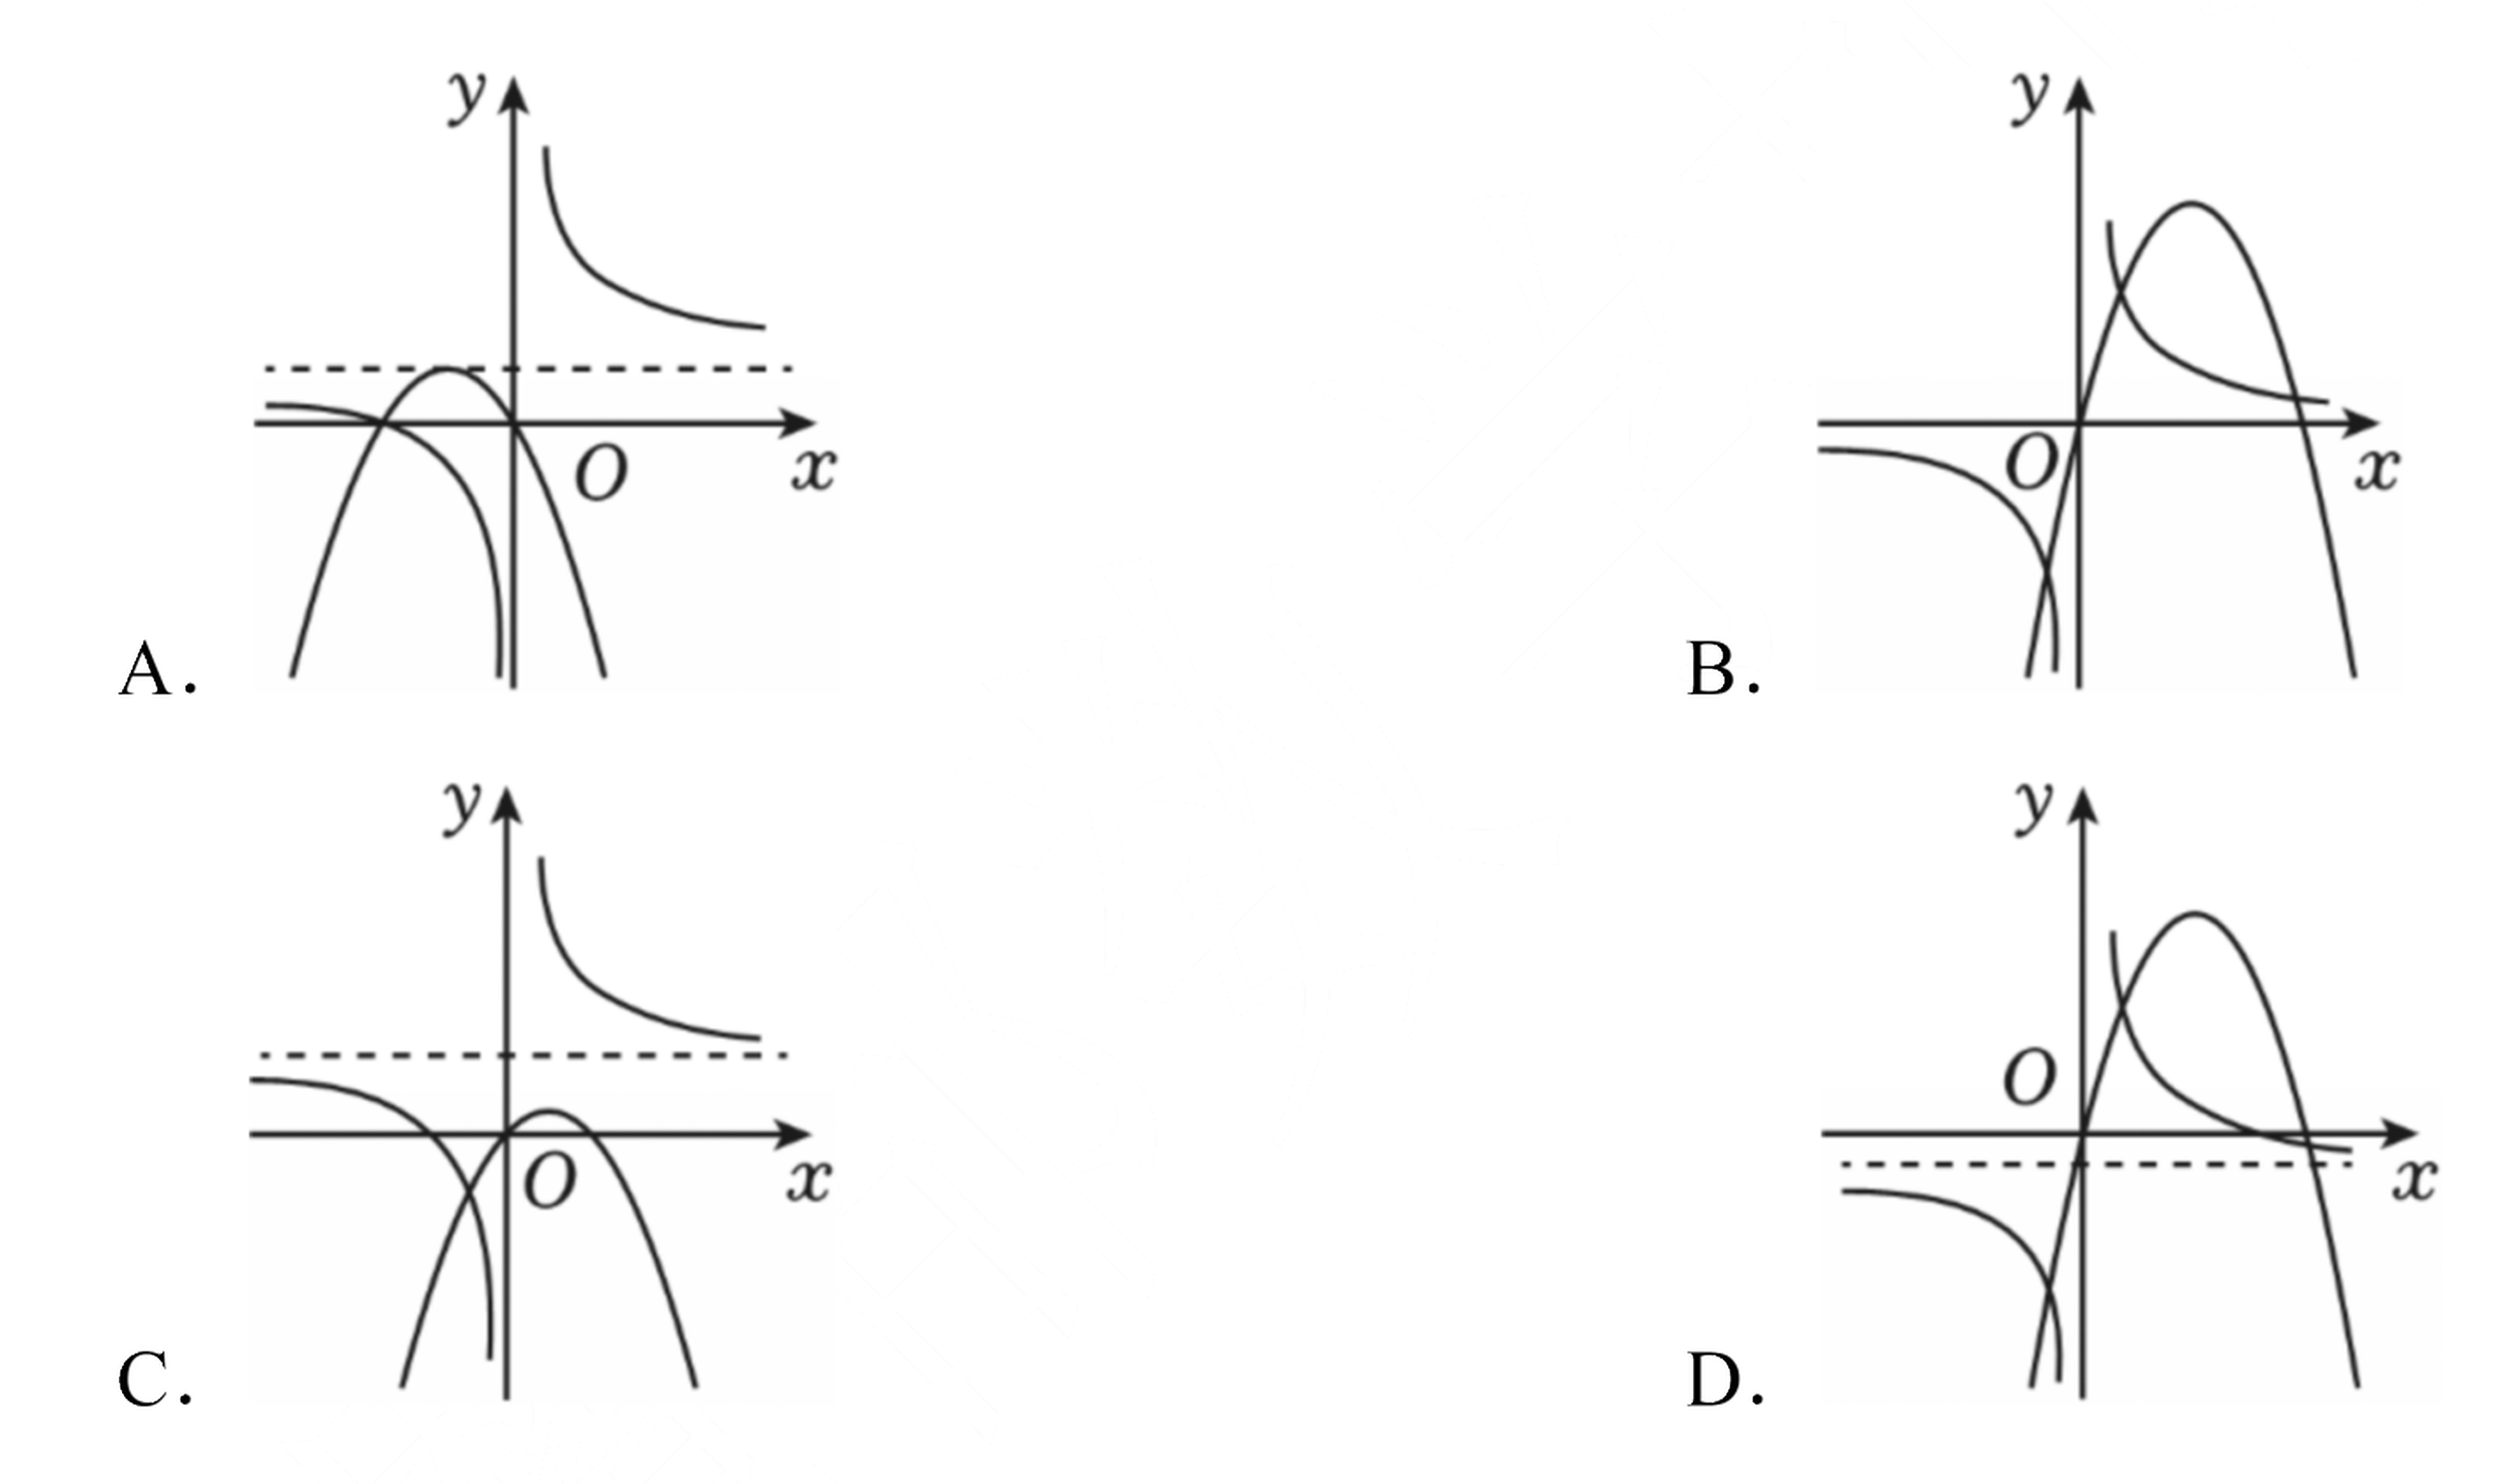
\includegraphics[width=0.80\textwidth]{figures/gao161_q14.png}
\end{center}

\ifanswer
\solbegin
\step{$A$ 选项，由二次函数图象得 $a<0$，$b<0$，由幂函数型函数图象得 $a<0$，$b>0$，}
\step{故 $A$ 选项错误；}
\step{$B$ 选项，由二次函数图象得 $a<0$，$b>0$，由幂函数型函数图象得 $a<0$，$b=0$，}
\step{故 $B$ 选项错误；}
\step{$C$ 选项，由二次函数图象得 $a<0$，$b>0$，由幂函数型函数图象得 $a<0$，$b>0$，}
\step{故 $C$ 选项正确；}
\step{$D$ 选项，由二次函数图象得 $a<0$，$b>0$，由幂函数型函数图象得 $a<0$，$b<0$，}
\step{故 $D$ 选项错误.}
\step{故选 $C$.}
\solend
\fi

% === Q15 === \subseteq／\subset、\varnothing、\mid；"排除 C""排除 B、D"正体字母照录；解析 4 行，故选 $A$
\item 设不等式 $\lvert f(x)\rvert+\lvert g(x)\rvert<a$（常数 $a>0$）的解集是 $M$，设不等式 $\lvert f(x)+g(x)\rvert<a$（常数 $a>0$）的解集是 $N$，则\mbox{（\quad）}

\keepwithprev
A. $M\subseteq N$\qquad B. $N\subseteq M$\qquad C. $M\subset N$\qquad D. $N\subset M$

\ifanswer
\solbegin
\step{$x\in M\Rightarrow\lvert f(x)+g(x)\rvert\leqslant\lvert f(x)\rvert+\lvert g(x)\rvert<a\Rightarrow x\in N$，所以 $M\subseteq N$.}
\step{取 $f(x)=g(x)=0$，则 $M=N$，排除 C.}
\step{取 $f(x)=1$，$g(x)=-1$，$a=1$，则 $M=\varnothing$，$N$ 为全体实数，排除 B、D.}
\step{故选 $A$.}
\solend
\fi

% === Q16 === "人文集"定义证明；cases 无；解析 21 行，故选 $B$
\item 设集合 $I_n=\{1,2,\cdots,n\}$，$n\in\N,n\geqslant1$，集合 $P_n=\left\{\dfrac{m}{\sqrt k}\mid m\in I_n,k\in I_n\right\}$，若 $P_n$ 的子集 $A$ 中任意两个元素之和不是整数的平方，则称 $A$ 为 “人文集”. 那么使 $P_n$ 能分成两个交集为空集的 “人文集” 的并集，且这两个人文集的并集恰为 $P_n$ 时，$n$ 的最大值是\mbox{（\quad）}

\keepwithprev
A. 13\qquad B. 14\qquad C. 15\qquad D. 16

\ifanswer
\solbegin
\step{先证当 $n\geqslant15$ 时，$P_n$ 不能分成两个不相交的人文集的并集.}
\step{假设当 $n\geqslant15$ 时，$P_n$ 可以分成两个不相交的人文集的并集，}
\step{设 $A$ 和 $B$ 为两个不相交的人文集，使 $A\cup B=P_n\supseteq I_n$.}
\step{不妨设 $1\in A$，则由于 $1+3=2^2$，所以 $3\notin A$，即 $3\in B$.}
\step{同理可得，$6\in A$，$10\in B$. 又推出 $15\in A$，}
\step{但 $1+15=4^2$，这与 $A$ 为人文集相矛盾.}
\step{再证 $P_{14}$ 满足要求. 当 $k=1$ 时，$P_{14}=\left\{\dfrac{m}{\sqrt k}\mid m\in I_{14},k\in I_{14}\right\}$，}
\step{可以分成 2 个人文集的并集.}
\step{事实上，只要取 $A_1=\{1,2,4,6,9,11,13\}$，$B_1=\{3,5,7,8,10,12,14\}$，}
\step{则 $A_1$ 和 $B_1$ 都是人文集，且 $A_1\cup B_1=P_{14}$.}
\step{当 $k=4$ 时，集合 $\left\{\dfrac{m}{\sqrt k}\mid m\in I_{14}\right\}$ 中，除整数外，}
\step{剩下的数组成集合 $\left\{\dfrac12,\dfrac32,\dfrac52,\cdots,\dfrac{13}{2}\right\}$，}
\step{可以分为下列 2 个人文集的并：$A_2=\left\{\dfrac12,\dfrac52,\dfrac92,\dfrac{11}{2}\right\}$，$B_2=\left\{\dfrac32,\dfrac72,\dfrac{13}{2}\right\}$.}
\step{当 $k=9$ 时，集合 $\left\{\dfrac{m}{\sqrt k}\mid m\in I_{14}\right\}$ 中，除整数外，}
\step{剩下的数组成集合 $\left\{\dfrac13,\dfrac23,\dfrac43,\dfrac53,\cdots,\dfrac{13}{3},\dfrac{14}{3}\right\}$，}
\step{可以分为下列 2 个人文集的并：$A_3=\left\{\dfrac13,\dfrac43,\dfrac53,\dfrac{10}{3},\dfrac{13}{3}\right\}$，$B_3=\left\{\dfrac23,\dfrac73,\dfrac83,\dfrac{11}{3},\dfrac{14}{3}\right\}$.}
\step{最后，集合 $C=\left\{\dfrac{m}{\sqrt k}\mid m\in I_{14},k\in I_{14},k\ne1,4,9\right\}$ 中的数的分母都是无理数，}
\step{它与 $P_n$ 中的任何其他数之和都不是整数，}
\step{因此，令 $A=A_1\cup A_2\cup A_3\cup C$，$B=B_1\cup B_2\cup B_3$，}
\step{则 $A$ 和 $B$ 是不相交的人文集，且 $A\cup B=P_{14}$.}
\step{综上，$n$ 的最大值为 14，故选 $B$.}
\solend
\fi

\end{enumerate}

\bigsec{三、解答题}

\begin{enumerate}
\setcounter{enumi}{16}

% === Q17 === "图像"照录；\Z；cases 块；解析 9 行，跨 06—07 页
\item (1) 已知函数 $y=x^{\frac{4m-m^2}{2}}$（$m\in\Z$）在区间 $(0,+\infty)$ 上是严格增函数，它的图像关于 $y$ 轴对称，求 $m$ 的值及该函数的解析式；

(2) 若 $(a-2)^{\frac32}<(1+2a)^{\frac32}$，求实数 $a$ 的取值范围.

\ifanswer
\solbegin
\step{(1) 由幂函数在 $(0,+\infty)$ 上严格递增，得 $\dfrac{4m-m^2}{2}>0\Leftrightarrow0<m<4$，}
\step{又 $m\in\Z$，所以 $m\in\{1,2,3\}$.}
\step{当 $m=1$ 或 $m=3$ 时，函数为 $y=x^{\frac32}$，定义域为 $[0,+\infty)$，}
\step{图像不关于 $y$ 轴对称.}
\step{当 $m=2$ 时，函数为 $y=x^2$，满足题意，所以 $m=2$，解析式 $y=x^2$.}
\step{(2) 原不等式有意义，须满足 $\begin{cases}a-2\geqslant0\\1+2a\geqslant0\end{cases}\Leftrightarrow a\geqslant2$，}
\step{函数 $y=x^{\frac32}$ 在 $[0,+\infty)$ 上严格递增，}
\step{因此 $(a-2)^{\frac32}<(1+2a)^{\frac32}\Leftrightarrow a-2<1+2a\Leftrightarrow a>-3$，}
\step{结合 $a\geqslant2$，得 $a\in[2,+\infty)$.}
\solend
\fi

% === Q18 === 题干"$a\geqslant0$"与解析"$a<0$"自相矛盾照录；"$A\cap B=(-2,-1]\cap[2,6)$"误印 ∩ 照录；\subseteq；解析 10 行
\item 已知实数 $a\geqslant0$，集合 $A=\left\{x\mid\dfrac{x+2}{x-6}<0\right\}$，$B=\{x\mid\lvert2x-1\rvert\geqslant3\}$，$C=\{x\mid x^2-3ax+2a^2<0\}$，

(1) 求 $A\cap B$；

(2) 若 $C\subseteq(A\cap B)$，求 $a$ 的取值范围.

\ifanswer
\solbegin
\step{(1) 由 $\dfrac{x+2}{x-6}<0$ 得 $-2<x<6$，即 $A=\{x\mid-2<x<6\}=(-2,6)$，}
\step{由 $\lvert2x-1\rvert\geqslant3$ 得 $2x-1\geqslant3$ 或 $2x-1\leqslant-3$，解得 $x\geqslant2$ 或 $x\leqslant-1$，}
\step{即 $B=(-\infty,-1]\cup[2,+\infty)$，}
\step{所以 $A\cap B=(-2,-1]\cap[2,6)$；}% 原卷把 ∪ 误印成 ∩，照录未改（见 ⑤ 2）
\step{(2) 由 (1) 得 $A\cap B=\{x\mid-2<x\leqslant-1\text{ 或 }2\leqslant x<6\}$，}
\step{因为 $C\subseteq(A\cap B)$，$x^2-3ax+2a^2=(x-a)(x-2a)<0$，}% 题干 $a\geqslant0$ 与解析 $a<0$ 自相矛盾，照录未改（见 ⑤ 1）
\step{当 $a=0$ 时，$C=\varnothing$，符合题意；}
\step{当 $a>0$ 时，$C=(a,2a)$，则 $\begin{cases}a\geqslant2\\2a\leqslant6\\a>0\end{cases}$，解得 $2\leqslant a\leqslant3$，}
\step{当 $a<0$ 时，$C=(2a,a)$，则 $\begin{cases}2a\geqslant-2\\a\leqslant-1\\a<0\end{cases}$，解得 $a=-1$，}
\step{故 $a$ 的范围为 $\{-1,0\}\cup[2,3]$.}
\solend
\fi

% === Q19 === 双碳太阳能应用题；"双碳""自发自用、市电互补"弯引号；解析 8 行，跨 08 页上下
\item 为响应 “双碳” 目标，某电子企业拟安装一套可使用 10 年的太阳能供电设备. 该设备的安装费用 $P(x)$（单位：万元）与太阳能电池板面积 $x(x>0)$（单位：平方米）成正比，比例系数为 $\dfrac12$. 为保障生产用电，安装后采用 “自发自用、市电互补” 模式，在此模式下，企业每年消耗的电费 $Q(x)$（单位：万元）与安装的这种太阳能电池板的面积 $x$ 之间的函数关系是 $Q(x)=\dfrac{180}{x+5}$. 记 $W(x)$（单位：万元）为该企业安装这种太阳能供电设备的费用与 10 年所消耗的电费之和.

(1) 要使该设备的安装费与第 1 年的电费之和不超过 17 万元，求安装太阳能电池板面积 $x$ 的取值范围；

(2) 当 $x$ 为多少平方米时，$W(x)$ 取得最小值？最小值是多少万元？

\ifanswer
\solbegin
\step{(1) $P(x)=\dfrac{x}{2}$，安装费与第 1 年的电费之和不超过 17 万元，即 $\dfrac{x}{2}+\dfrac{180}{x+5}\leqslant17$，}
\step{$x>0$，上式等价于 $x^2-29x+190\leqslant0\Leftrightarrow(x-10)(x-19)\leqslant0$，}
\step{解得 $x\in[10,19]$.}
\step{(2) 安装费用与 10 年电费之和为 $W(x)=P(x)+10Q(x)$，}
\step{$=\dfrac{x}{2}+\dfrac{1800}{x+5}=\dfrac{x+5}{2}+\dfrac{1800}{x+5}-\dfrac52$，}
\step{$x>0$，由基本不等式得 $W(x)\geqslant2\sqrt{\dfrac{x+5}{2}\cdot\dfrac{1800}{x+5}}-\dfrac52=60-\dfrac52=57.5$，}
\step{等号当且仅当 $\dfrac{x+5}{2}=\dfrac{1800}{x+5}$，即 $x=55$ 时成立.}
\step{因此，当电池板面积为 55 平方米时，$W(x)$ 取得最小值 57.5 万元.}
\solend
\fi

% === Q20 === $a*b$ 定义；\min 改正体；cases 块；解析 23 行，跨 08—10 页
\item 设 $a$、$b\in\R$，定义 $a*b=\begin{cases}a,&a<b\\b,&a\geqslant b\end{cases}$.

(1) 若 $x*2>1$，求 $x$ 的取值范围；

(2) 若 $(\lvert x-1\rvert+\lvert x-2\rvert)*3=3$，求 $x$ 的取值范围；

(3) 若 $a$、$b>0$，记 $M=a*\dfrac{b}{a^2+4b^2}$，分别比较 $M$ 与 $a$，以及 $M$ 与 $\dfrac{b}{a^2+4b^2}$ 的大小，并求 $M$ 的最大值.

\ifanswer
\solbegin
\step{(1) 定义 $a*b=\begin{cases}a,&a<b\\b,&a\geqslant b\end{cases}$，由 $x*2>1$，得 $\begin{cases}x<2\\x>1\end{cases}$，或 $\begin{cases}x\geqslant2\\2>1\end{cases}$，}
\step{解得 $x>1$，即 $x$ 的取值范围为 $\{x\mid x>1\}$；}
\step{(2) 当 $x\geqslant2$ 时，$\lvert x-1\rvert+\lvert x-2\rvert=2x-3\geqslant1$，}
\step{当 $1\leqslant2x-3\leqslant3$，即 $2\leqslant x\leqslant3$ 时，}
\step{此时 $(\lvert x-1\rvert+\lvert x-2\rvert)*3=2x-3=3$，解得 $x=3$；}
\step{当 $2x-3>3$，即 $x>3$ 时，}
\step{此时 $(\lvert x-1\rvert+\lvert x-2\rvert)*3=3$ 恒成立，则 $x>3$；}
\step{当 $-2x+3>3$，即 $x<0$ 时，}
\step{此时 $(\lvert x-1\rvert+\lvert x-2\rvert)*3=3$ 恒成立，则 $x<0$.}
\step{当 $1<x<2$ 时，$\lvert x-1\rvert+\lvert x-2\rvert=1$，}
\step{此时 $(\lvert x-1\rvert+\lvert x-2\rvert)*3=1\ne3$，不符合题意；}
\step{当 $x\leqslant1$ 时，$\lvert x-1\rvert+\lvert x-2\rvert=-2x+3\geqslant1$，}
\step{当 $-2x+3\leqslant3$，即 $0\leqslant x\leqslant1$ 时，}
\step{此时 $(\lvert x-1\rvert+\lvert x-2\rvert)*3=-2x+3=3$，解得 $x=0$.}
\step{综上所述，$x$ 的取值范围为 $\{x\mid x\leqslant0\text{ 或 }x\geqslant3\}$；}
\step{(3) 由题意，$M=a*\dfrac{b}{a^2+4b^2}=\min\left\{a,\dfrac{b}{a^2+4b^2}\right\}$，}% 原卷印斜体 min，按全稿惯例改正体 \min（见 ② ⑬）
\step{则 $M\leqslant a$，$M\leqslant\dfrac{b}{a^2+4b^2}$.}
\step{因为 $a$、$b>0$，所以 $\dfrac{b}{a^2+4b^2}\leqslant\dfrac{b}{2\sqrt{a^2\cdot4b^2}}=\dfrac{1}{4a}$，}
\step{当且仅当 $a=2b>0$ 时取等号，}
\step{当 $a\geqslant\dfrac{1}{4a}$，即 $a\geqslant\dfrac12$ 时，$M=a*\dfrac{b}{a^2+4b^2}=\dfrac{b}{a^2+4b^2}\leqslant\dfrac{1}{4a}$，}
\step{则 $a=\dfrac12$，$b=\dfrac14$ 时，$M$ 取得最大值 $\dfrac12$；}
\step{当 $0<a<\dfrac12$ 时，$M=a*\dfrac{b}{a^2+4b^2}=a$，此时 $M<\dfrac12$.}
\step{综上所述，$M$ 的最大值为 $\dfrac12$.}
\solend
\fi

% === Q21 === $A_n$／$B_n$／$S_n$／$T_n$ 新定义；题干第 3 问误标 (2) 照录、解析作 (3)；\prec；解析 25 行，跨 10—11 页
\item 对任意正整数 $n$，记集合 $A_n=\{(a_1,a_2,\cdots,a_n)\mid a_1,a_2,\cdots,a_n$ 均为非负整数，且 $a_1+a_2+\cdots+a_n=n\}$，集合 $B_n=\{(b_1,b_2,\cdots,b_n)\mid b_1,b_2,\cdots,b_n$ 均为非负整数，且 $b_1+b_2+\cdots+b_n=2n\}$. 设 $\alpha=(a_1,a_2,\cdots,a_n)\in A_n$，$\beta=(b_1,b_2,\cdots,b_n)\in B_n$，若对任意 $i\in\{1,2,\cdots,n\}$ 都有 $a_i\leqslant b_i$，则记 $\alpha\prec\beta$.

(1) 写出集合 $A_2$ 和 $B_2$；

(2) 证明：对任意 $\alpha\in A_n$，存在 $\beta\in B_n$，使得 $\alpha\prec\beta$；

(2) 设集合 $S_n=\{(\alpha,\beta)\mid\alpha\in A_n,\beta\in B_n,\alpha\prec\beta\}$，求证：$S_n$ 中的元素个数是完全平方数.% 原卷第 3 问题干误标 (2)（与第 2 问重号），照录未改（见 ⑤ 3）

\ifanswer
\solbegin
\step{(1) $A_2=\{(0,2),(1,1),(2,0)\}$，$B_2=\{(0,4),(1,3),(2,2),(3,1),(4,0)\}$；}
\step{(2) 对任意 $\alpha=(a_1,a_2,\cdots,a_n)\in A_n$，设 $b_i=a_i+1$（$i=1,2,3,\cdots,n$），}
\step{则 $b_1,b_2,\cdots,b_n$ 均为非负整数，且 $a_i\leqslant b_i$（$i=1,2,3,\cdots,n$）.}
\step{令 $\beta=(b_1,b_2,\cdots,b_n)$，则 $b_1+b_2+\cdots+b_n$}
\step{$=(a_1+1)+(a_2+1)+\cdots+(a_n+1)=(a_1+a_2+\cdots+a_n)+n=2n$，}
\step{所以 $\beta\in B_n$，且 $\alpha\prec\beta$.}
\step{(3) 对任意 $\alpha=(a_1,a_2,\cdots,a_n)\in A_n$，$\alpha'=(a_1',a_2',\cdots,a_n')\in A_n$，}
\step{记 $\alpha+\alpha'=(a_1+a_1',a_2+a_2',\cdots,a_n+a_n')$，}
\step{则 $a_1+a_1',a_2+a_2',\cdots,a_n+a_n'$ 均为非负整数，}
\step{且 $(a_1+a_1')+(a_2+a_2')+\cdots+(a_n+a_n')$}
\step{$=(a_1+a_2+\cdots+a_n)+(a_1'+a_2'+\cdots+a_n')=n+n=2n$，}
\step{所以 $\alpha+\alpha'\in B_n$，且 $\alpha\prec\alpha+\alpha'$，$\alpha'\prec\alpha+\alpha'$.}
\step{设集合 $A_n$ 中的元素个数为 $t$，设 $A_n=\{\alpha_1,\alpha_2,\cdots,\alpha_t\}$.}
\step{设集合 $T_n=\{(\alpha_i,\alpha_i+\alpha_j)\mid i=1,2,\cdots,t,j=1,2,\cdots,t\}$.}
\step{对任意 $\alpha_i\in A_n$（$i=1,2,\cdots,t$），都有 $\alpha_i+\alpha_1,\alpha_i+\alpha_2,\cdots,\alpha_i+\alpha_t\in B_n$，}
\step{且 $\alpha_i\prec\alpha_i+\alpha_j$，$j=1,2,\cdots,t$，所以 $T_n\subseteq S_n$.}
\step{若 $(\alpha,\beta)\in S_n$，其中 $\alpha=(a_1,a_2,\cdots,a_n)\in A_n$，$\beta=(b_1,b_2,\cdots,b_n)\in B_n$，}
\step{设 $c_i=b_i-a_i$（$i=1,2,\cdots,n$），因为 $a_i\leqslant b_i$，所以 $c_i=b_i-a_i\geqslant0$，}
\step{记 $\alpha'=(c_1,c_2,\cdots,c_n)$，}
\step{则 $c_1+c_2+\cdots+c_n=(b_1-a_1)+(b_2-a_2)+\cdots+(b_n-a_n)$}
\step{$=(b_1+b_2+\cdots+b_n)-(a_1+a_2+\cdots+a_n)=2n-n=n$，}
\step{所以 $\alpha'\in A_n$，并且有 $\beta=\alpha+\alpha'$，所以 $(\alpha,\beta)\in T_n$，所以 $S_n\subseteq T_n$，}
\step{所以 $S_n=T_n$.}
\step{因为集合 $T_n$ 中的元素个数为 $t^2$，所以 $S_n$ 中的元素个数为 $t^2$，}
\step{是完全平方数.}
\solend
\fi

\end{enumerate}

\end{document}
"
% 紧凑版：xelatex "\def\iscompact{1}% 高一161_松江一中嘉一实验_期中.tex
%   —— 高一上数学"2026-2027 年松江一中嘉一实验高一上期中"（试卷版/答案版/紧凑版）
% 试卷版：xelatex 高一161_松江一中嘉一实验_期中.tex
% 答案版：xelatex "\def\isanswer{1}% 高一161_松江一中嘉一实验_期中.tex
%   —— 高一上数学"2026-2027 年松江一中嘉一实验高一上期中"（试卷版/答案版/紧凑版）
% 试卷版：xelatex 高一161_松江一中嘉一实验_期中.tex
% 答案版：xelatex "\def\isanswer{1}\input{高一161_松江一中嘉一实验_期中.tex}"
% 紧凑版：xelatex "\def\iscompact{1}\input{高一161_松江一中嘉一实验_期中.tex}"
%
% ① 原始材料：微信公众号"魔都数学加油站"文章，连载"27学年高一161"，原卷卷面标题
% "2026-2027 年松江一中嘉一实验高一上期中"（卷面未印副标题、未印连载号）。
% 正文为 11 张 PNG 页（01/02/03/05/06/07/08/09/11 为 4762×6735，04/10 为
% 2560×3620，同一篇各页分辨率混排，逐页按各自分辨率裁图核对）。
% 体例：讲评版——填空 3—12（10 题）、选择 13—16（4 题）、解答 17—21（5 题），
% 共 19 题，自第 3 题起编（1、2 未印在本篇）；Q13 答案"A"直接印在题干括号内、
% 且无【答案】/【解析】段，本稿按 高一37 第 13 题／高一57 第 13 题成例把括号
% 留空、另提 \ans{$A$}；其余 18 题逐题印【解析】、用 \solbegin…\solend。
% 题目、答案、解析均据原图转录；卷面粉红色水印"魔都数学加油站"及公众号页脚未录入。
% 全卷插图清单（逐页通读 11 页确认）：仅 1 组——Q14 四幅图像选项（04 页 2×2
% 排布，二次函数与幂函数型函数在同一坐标系中的图象，A/B/C/D 四幅小图），
% 合并成一张，三版都出，裁 figures/gao161_q14.png。其余各页逐页确认无其它
% 题目配图、无解析内配图、无表格、无"如图"处（Q16 解析里的"可以分为下列 2 个
% 人文集的并"是纯文字＋集合，不是表格；OCR 里看似表格的行实为大括号与分数）。
%
% 卷首标题：原卷印作"2026-2027 年松江一中嘉一实验高一上期中"，年份区间按全稿惯例排 en dash；
% 原卷卷面未印副标题，本稿按同期中卷知识模块口径补出"集合与常用逻辑用语、不等式、函数"。
%
% ② 与原卷的排版差异／照录项清单：
%   ① 原文从第 3 题起，本稿保留原题号；共 19 题三节，解答题 5 题到 21；
%      三节各自一个 enumerate + \setcounter{enumi}{2}/{12}/{16}（不贯穿），
%      用 \examtitlest[3] 起手；
%   ② 混合体例：Q13 原卷把答案"A"直接印在题干括号内（"（  A  ）"）、且题下
%      无【答案】/【解析】段，按 高一37 第 13 题／高一57 第 13 题成例把括号
%      留空、另提 \ans{$A$}、不补造解析；其余 18 题印【解析】、用
%      \solbegin…\solend；四道选择题中 Q14/Q15/Q16 的答案在解析末句
%      "故选 $C$／$A$／$B$"、Q13 用 \ans{$A$}；括号 \mbox{（\quad）} 留空；
%      答案版【答案】/【解析】标记数 = 19 = 全卷题数（1 个 \ans ＋ 18 个 \solbegin）；
%   ③ 原卷卷面未印副标题，本稿按知识模块口径补出；
%   ④ 原卷填空横线按全稿惯例排 \blankline[4.4em]；选择题选项段前按惯例各加
%      \keepwithprev；Q14 四幅选项图整块用 \needvspace{9cm} 守卫（守卫放
%      \item 之前，见 高一132 Q14／高一154 Q15 成例）；解答题不留作答区、
%      不加 \anspace（原卷为讲评版）；
%   ⑤ 数集归一：Q8"$x\in\R$"、Q11"$m\in\R$"、Q13"$x,y\in\N$"、
%      Q16"$n\in N$"、Q17"$m\in\Z$"、Q20"$a$、$b\in R$"——原卷印正体粗体
%      或斜体 R/N/Z，按全稿惯例归一 \R／\N／\Z；绝对值排 \lvert…\rvert
%      （Q9、Q12、Q15、Q18、Q20），集合描述竖线排 \mid（Q12、Q16、Q18、
%      Q20、Q21），空集 \varnothing（Q15、Q18），补集无用例，不等号按全稿
%      惯例排 \leqslant／\geqslant；
%   ⑥ 子集符号逐处照录不统一：Q12 cases 定义"$C(A)\geqslant C(B)$"、
%      Q15 选项 A/B"$M\subseteq N$""$N\subseteq M$"与解析"$M\subseteq N$"
%      印带下划线 ⊆（照录 \subseteq），Q15 选项 C/D"$M\subset N$""$N\subset M$"
%      印单线 ⊂（照录 \subset），Q18 "$C\subseteq(A\cap B)$"、Q21
%      "$T_n\subseteq S_n$""$S_n\subseteq T_n$"均带下划线照录 \subseteq；
%      本卷无 \not\subset 用例；
%   ⑦ 判别式：Q7 解析"$\Delta=(m-6)(m+2)>0$"、Q8 解析"$\Delta=a^2-4a<0$"、
%      Q12 解析"$\Delta=a^2-8$"共 3 处，逐处放大确认印等腰偏高粗三角
%      （高>宽、右斜边粗），照录 \Delta；本卷无扁等边细线 \triangle 用例；
%   ⑧ 中文弯引号照录：Q7"$m\geqslant6$""有两个不相等的正实数根"及四个
%      条件短语、Q13 反证法命题、Q16"人文集"、Q19"双碳""自发自用、市电互补"；
%      注释里一律 ASCII 引号；数学式内 CJK 用 \text{}（Q18、Q20 解集描述内"或"）；
%   ⑨ "图像／图象"逐处照录不统一：Q4"的图像"、Q17 题干"它的图像关于 $y$ 轴
%      对称"及解析"图像不关于 $y$ 轴对称"印"图像"；Q14 题干"的图象可能为"
%      与解析 A/B/C/D 四行各"由二次函数图象得""由幂函数型函数图象得"
%      共 8 处印"图象"（象，无亻）；
%   ⑩ 文本圈数字逐处照录：Q12 题干①②③④、Q12 解析"故①错误""故②正确"
%      "故③正确""故④错误""故正确的是②③"，均为印刷圈数字（文本模式）；
%   ⑪ 半角逗号在数学组之间是全稿惯例、非笔误，逐处照录（Q5"$a$、$b$"、
%      Q13"$x,y\in\N$"、Q16"$n\in\N,n\geqslant1$"与集合描述内逗号、
%      Q20"$a,b\in\R$"、Q21 各集合描述内逗号）；行末西文句点 ASCII `.`；
%      原卷行中句点（Q16"$10\in B$. 又推出 $15\in A$"、Q16"再证 $P_{14}$
%      满足要求. 当 $k=1$ 时"、Q18"$A\cap B=(-2,-1]\cap[2,6)$；"后的分号）
%      按全稿惯例一律排 ASCII `.`／全角"；"；中文语境行中全角逗号／顿号照录；
%   ⑫ 原卷数学式内联条件（Q14"$y=x^a+b(a\ne0)$"、Q19"$x(x>0)$"、
%      Q11"$\lvert x-m\rvert<n\,(m\in\R,n>0)$"）印半角括号，逐处照录未改
%      全角（同 高一147 口径）；
%      中文语境的括注（Q5"结果用 $a$、$b$ 表示"、Q7"填…"、Q12"填写序号"、
%      Q15"常数 $a>0$"、Q19"单位：万元"）印全角括号，照录；
%   ⑬ 复杂式照录别简化：Q3 $(a^{2-\sqrt3})^{2+\sqrt3}\times\sqrt{a^2}\times
%      b^{\sqrt3}\times b^{1-\sqrt3}$ 与 $a^{(2-\sqrt3)(2+\sqrt3)}\cdot a\cdot
%      b^{\sqrt3+1-\sqrt3}=a\cdot a\cdot b=a^2b$（题干用 \times、解析用 \cdot，
%      逐处照录不统一，见 ⑤）；Q5 $\dfrac{\lg2}{\lg2+\lg3}=\dfrac{a}{a+b}$、
%      Q10 $t-\dfrac3t=2$ 与 $b=a^3$、$ab=a^4=2$、Q11 $\left(2a-\dfrac12
%      -a+\dfrac12,2a-\dfrac12+a-\dfrac12\right)=(a,3a-1)$ 与
%      $\left(\dfrac43,\dfrac53\right]\cup\{2\}$、Q16 各分数集合、Q19
%      $x^2-29x+190\leqslant0$ 与 $W(x)=P(x)+10Q(x)$ 与
%      $2\sqrt{\dfrac{x+5}{2}\cdot\dfrac{1800}{x+5}}-\dfrac52=60-\dfrac52=57.5$、
%      Q20 $M=a*\dfrac{b}{a^2+4b^2}=\min\left\{a,\dfrac{b}{a^2+4b^2}\right\}$
%      与 $\dfrac{b}{2\sqrt{a^2\cdot4b^2}}=\dfrac{1}{4a}$、Q21 各 $A_n$／$B_n$／
%      $T_n$ 定义；\left…\right 不得拆到不同 $…$ 组（Q11 的 \left(…\right)、
%      Q11 的 \left(\dfrac43,\dfrac53\right]、Q16 的 \left\{\dfrac{m}{\sqrt k}
%      \mid…\right\} 与 \left\{\dfrac12,\dfrac32,\dfrac52,\cdots,\dfrac{13}{2}\right\}
%      等、Q20 的 \min\left\{…\right\}）；cases 块整体算一个印刷行
%      （Q12 定义、Q17 (2)、Q18 (2) 两处、Q20 定义与 (1)）；原卷 Q20 解析
%      "$=min\{…\}$"印斜体 min，按 高一122／高一102 成例改正体 \min；
%   ⑭ 一条 \step = 原卷解析的一个印刷行；别并折行、别拆行。跨页续印按题合并
%      （Q6 的 01 页上下题干重复印、Q10 的 01—02 页、Q11 的 02—03 页、
%      Q12 的 03—04 页、Q16 的 05—06 页、Q17 的 06—07 页、Q18 的 07 页
%      上下、Q19 的 08 页上下、Q20 的 08—10 页、Q21 的 10—11 页）；
%      跨半页重叠行（Q10"令 $t=\log_a b>0$…"、Q16"它与 $P_n$ 中的任何
%      其他数之和都不是整数，"、Q18"【解析】(1) 由 $\dfrac{x+2}{x-6}<0$…"、
%      Q19"$x>0$，上式等价于…"、Q20"此时…则 $x<0$."、Q21"若 $(\alpha,\beta)
%      \in S_n$…"与"设 $c_i=b_i-a_i$…"）只算一个印刷行；
%   ⑮ 自定义记号照录：Q12"$C(A)$""$A*B$""$S$"、Q16"$I_n$""$P_n$""人文集"
%      "$A_1$／$B_1$／$A_2$／$B_2$／$A_3$／$B_3$／$C$"、Q20"$a*b$""$M$"、
%      Q21"$A_n$／$B_n$／$S_n$／$T_n$""$\alpha\prec\beta$""$\alpha+\alpha'$"；
%   ⑯ 选项字母体例照录不统一：Q15 解析"排除 C.""排除 B、D."两处原卷印
%      正体（文本模式），Q13 \ans{$A$}、Q14"$A$ 选项"…"故选 $C$"、
%      Q15"故选 $A$"、Q16"故选 $B$"用斜体（数学模式），逐处照录、不统一；
%   ⑰ 红字：全卷逐页扫描无红色加粗小标题（仅粉色水印），故本卷无 \stepm，
%      不引入红色定义；
%
% ③ 行数复核：一条 \step = 原卷解析的一个印刷行，cases 块作一个印刷行计。
%   逐题数（逐页核对定稿）：Q3：1；Q4：1；Q5：1；Q6：3；Q7：4；Q8：4；
%   Q9：2；Q10：2；Q11：7；Q12：8；Q13：0（答案印括号内、提 \ans{}，
%   不计入 \step 账）；Q14：9；Q15：4；Q16：21；Q17：9；Q18：10；Q19：8；
%   Q20：23；Q21：25。
%   合计 142 行（142 条 \step，无 \stepm），与原卷逐题印刷行相等。
%   全卷 19 题：Q13 一处 \ans{} ＋ 其余 18 题设 \solbegin…\solend，
%   答案版【答案】/【解析】标记数 = 19 = 全卷题数。
%
% ④ 页码分布（供回原图复核）：
%   卷首标题＋"一、填空题"＋Q3/Q4/Q5 题干＋解析各 1 行＋Q6 题干首行
%   在 01 页上半；Q6 题干（重复印）＋解析 3 行＋Q7 题干＋解析 4 行在
%   01 页下半；Q8 题干＋解析 4 行＋Q9 题干＋解析 2 行＋Q10 题干＋
%   解析首行在 02 页上半；Q10 解析（重复印）＋末行＋Q11 题干＋解析
%   前 3 行在 02 页下半；Q11 解析后 4 行＋Q12 题干＋cases 定义＋①
%   在 03 页上半；Q12 ②③④ 三命题＋"填写序号"行＋解析前 6 行在
%   03 页下半；Q12 解析后 2 行＋"二、选择题"标题＋Q13 题干＋选项＋
%   Q14 题干＋"（　）"＋A/B 两幅图在 04 页上半；Q14 四幅图（重复印）
%   ＋解析 9 行在 04 页下半；Q15 题干＋选项＋解析 4 行＋Q16 题干＋
%   选项在 05 页上半；Q16 题干（重复印）＋选项＋解析前 10 行在 05 页
%   下半；Q16 解析中 8 行（k=4、k=9 两批＋集合 C＋"它与 $P_n$…"）
%   在 06 页上半；Q16 解析"它与 $P_n$…"（重复印）＋末 3 行＋
%   "三、解答题"标题＋Q17 题干＋两问＋解析前 4 行在 06 页下半；
%   Q17 解析后 5 行＋Q18 题干＋两问＋解析首行在 07 页上半；Q18 解析
%   （重复首行）＋余 9 行在 07 页下半；Q19 题干＋两问＋解析前 2 行在
%   08 页上半；Q19 解析（重复第 2 行）＋余 6 行＋Q20 定义＋(1) 问在
%   08 页下半；Q20 (2)(3) 两问＋解析 (1) 2 行＋(2) 前 7 行在 09 页
%   上半；Q20 解析 (2) 余 4 行＋(3) 前 4 行在 09 页下半；Q20 解析 (3)
%   余 4 行＋Q21 题干＋三问在 10 页上半；Q21 题干（重复印）＋解析
%   (1)(2)(3) 前 8 行在 10 页下半；Q21 解析 (3) 中 10 行在 11 页上半；
%   Q21 解析 (3)（重复 2 行）＋末 7 行"是完全平方数."在 11 页下半。
%   本稿按题连排，不丢行、不并折行；全卷末题为第 21 题，无附加题节。
%
% ⑤ 存疑照录（放大原图确认，照录未改、正文对应处另有 % 注）：
%   1. Q18 题干印"已知实数 $a\geqslant0$"，解析却另设"当 $a<0$ 时"并解出
%      $a=-1$，末行答案"故 $a$ 的范围为 $\{-1,0\}\cup[2,3]$"含负数，
%      与题干 $a\geqslant0$ 自相矛盾——系原卷前后不一，照录未改（放大
%      07 页确认题干确印 $a\geqslant0$）；
%   2. Q18 解析"所以 $A\cap B=(-2,-1]\cap[2,6)$；"原卷把并集误印成
%      交集号 ∩（紧接下一行"$A\cap B=\{x\mid-2<x\leqslant-1$ 或
%      $2\leqslant x<6\}$"用"或"），照录未改（放大 07 页确认印 ∩）；
%   3. Q21 题干第 3 问原卷标号印作"(2)"（与第 2 问重号），而解析里
%      同一问标作"(3)"——原卷笔误，题干与解析逐处照录、不统一；
%   4. Q3 题干四处乘号印"×"（\times）、解析内三处乘号印"·"（\cdot），
%      逐处照录未统一（放大 01 页确认）；
%   5. Q16 解析"先证当 $n\geqslant15$ 时"印 ≥（非 >），与"综上，$n$
%      的最大值为 14"自洽，照录；题干"$n\in N,n\geqslant1$"印斜体
%      $N$、按全稿惯例归一 \N（见 ② ⑤）；
%   6. Q20 解析"$M=a*\dfrac{b}{a^2+4b^2}=min\{…\}$"原卷印斜体 min，
%      按全稿惯例改正体 \min（见 ② ⑬）；末行"$M$ 的最大值为
%      $\dfrac12$"照录；
%   7. Q15 解析"排除 C.""排除 B、D."用正体字母，而"故选 $A$"用斜体
%      字母，原卷体例不一（见 ② ⑯），照录未统一。
%   全卷除此 7 类外未发现其它笔误／自相矛盾处；Q13 只把答案印在括号内、
%   其余 18 题全部印【解析】。
%

\documentclass[a4paper,11pt]{article}
\usepackage{common}

\begin{document}

\examtitlest[3]{2026--2027 年松江一中嘉一实验高一上期中}{集合与常用逻辑用语、不等式、函数}

\bigsec{一、填空题}

\begin{enumerate}
\setcounter{enumi}{2}

% === Q3 === 题干 \times、解析 \cdot 逐处照录；解析 1 行
\item 设 $a>0$，$b>0$，化简 $(a^{2-\sqrt3})^{2+\sqrt3}\times\sqrt{a^2}\times b^{\sqrt3}\times b^{1-\sqrt3}=$\blankline[4.4em].

\ifanswer
\solbegin
\step{因为 $a>0$，所以 $\sqrt{a^2}=a$，原式 $=a^{(2-\sqrt3)(2+\sqrt3)}\cdot a\cdot b^{\sqrt3+1-\sqrt3}=a\cdot a\cdot b=a^2b$.}
\solend
\fi

% === Q4 === "图像"照录；解析 1 行
\item 若幂函数 $y=x^a$ 的图像经过点 $(5,\sqrt5)$，则此幂函数的表达式为 $y=$\blankline[4.4em].

\ifanswer
\solbegin
\step{$5^a=\sqrt5\Rightarrow a=\dfrac12$，所以 $y=\sqrt x$.}
\solend
\fi

% === Q5 === "结果用 $a$、$b$ 表示"全角括号＋顿号照录；解析 1 行
\item 已知 $\lg2=a$，$10^b=3$，则 $\log_6 2=$\blankline[4.4em]（结果用 $a$、$b$ 表示）.

\ifanswer
\solbegin
\step{$\lg3=b$，$\log_6 2=\dfrac{\lg2}{\lg2+\lg3}=\dfrac{a}{a+b}$.}
\solend
\fi

% === Q6 === 对称中心；解析 3 行，题干跨 01 页上下重复印
\item 若函数 $y=\dfrac{mx-1}{x+n}$ 的对称中心是 $(4,-3)$，则 $m+n=$\blankline[4.4em].

\ifanswer
\solbegin
\step{令 $x=-n+t$（$t\ne0$），则 $y-m=-\dfrac{mn+1}{t}$；}
\step{将 $t$ 换成 $-t$，$y-m$ 变为其相反数，因此对称中心为 $(-n,m)$.}
\step{于是 $n=-4$，$m=-3$，得 $m+n=-7$.}
\solend
\fi

% === Q7 === 充要条件；中文弯引号＋圈选条件；\Delta 高瘦；解析 4 行
\item 已知关于 $x$ 的一元二次方程 $x^2-mx+m+3=0$，则 “$m\geqslant6$” 是该方程 “有两个不相等的正实数根” 的\blankline[4.4em]条件（填 “充分不必要”、“必要不充分”、“充要” 或 “既不充分也不必要”）.

\ifanswer
\solbegin
\step{方程有两个不相等的正实数根}
\step{$\Leftrightarrow m>0$、$m+3>0$ 且 $\Delta=(m-6)(m+2)>0\Leftrightarrow m>6$.}
\step{$m>6\Rightarrow m\geqslant6$，但 $m=6$ 时方程有两个相等的正实数根，}
\step{因此为必要不充分条件.}
\solend
\fi

% === Q8 === \R、\Delta；解析 4 行
\item 对于任意的 $x\in\R$，代数式 $\lg(ax^2+ax+1)$ 都有意义，则实数 $a$ 的取值范围是\blankline[4.4em].

\ifanswer
\solbegin
\step{真数须满足 $ax^2+ax+1>0$ 对任意 $x\in\R$ 恒成立.}
\step{$a=0$ 时成立；}
\step{$a\ne0$ 时，恒成立等价于 $a>0$ 且 $\Delta=a^2-4a<0$，解得 $0<a<4$；}
\step{因此 $a\in[0,4)$.}
\solend
\fi

% === Q9 === 绝对值 \lvert…\rvert；解析 2 行
\item 若不等式 $\lvert x+1\rvert-\lvert x-4\rvert<m$ 的解集为非空集合，则实数 $m$ 的取值范围是\blankline[4.4em].

\ifanswer
\solbegin
\step{$\lvert x+1\rvert-\lvert x-4\rvert\geqslant-\lvert(x+1)-(x-4)\rvert=-5$，当 $x=-1$ 时取等号，}
\step{因此原不等式的解集非空 $\Leftrightarrow m>-5$，所求范围为 $(-5,+\infty)$.}
\solend
\fi

% === Q10 === 换底；$\log_2 a\cdot\log_2 b$；解析 2 行，跨 02 页上下
\item 已知 $a>1$，$b>1$，若 $\log_a b-3\log_b a=2$，且 $ab=2$，则 $\log_2 a\cdot\log_2 b=$\blankline[4.4em].

\ifanswer
\solbegin
\step{令 $t=\log_a b>0$，则 $t-\dfrac{3}{t}=2\Leftrightarrow(t-3)(t+1)=0$，得 $t=3$，}
\step{于是 $b=a^3$，$ab=a^4=2$，得 $\log_2 a=\dfrac14$，$\log_2 b=\dfrac34$，所求为 $\dfrac{3}{16}$.}
\solend
\fi

% === Q11 === 邻域定义；\left(…\right) 不拆组；解析 7 行，跨 02—03 页
\item 对于实数 $m$ 和正数 $n$，称满足不等式 $\lvert x-m\rvert<n\,(m\in\R,n>0)$ 的实数 $x$ 的集合叫做 $m$ 的 $n$ 邻域. 已知 $a>\dfrac12$，若 $2a-\dfrac12$ 的 $a-\dfrac12$ 邻域中恰有 2 个整数，则 $a$ 的取值范围是\blankline[4.4em].

\ifanswer
\solbegin
\step{所求邻域为 $\left(2a-\dfrac12-a+\dfrac12,2a-\dfrac12+a-\dfrac12\right)=(a,3a-1)$.}
\step{当 $\dfrac12<a\leqslant1$ 时至多含 1 个整数；}
\step{当 $a>2$ 时，区间长度 $2a-1>3$，至少含 3 个整数.}
\step{当 $1<a<2$ 时，区间必含 2，恰有两个整数等价于 $3<3a-1\leqslant4$，}
\step{即 $\dfrac43<a\leqslant\dfrac53$.}
\step{当 $a=2$ 时，区间为 $(2,5)$，恰含整数 $3,4$；}
\step{所以 $a\in\left(\dfrac43,\dfrac53\right]\cup\{2\}$.}
\solend
\fi

% === Q12 === $C(A)$／$A*B$ 定义题；①②③④ 文本圈数字；\subseteq／\subset、\Delta、\mid、\varnothing；解析 8 行
\item 用 $C(A)$ 表示非空集合 $A$ 中的元素个数. 对于集合 $A$、$B$，定义

$A*B=\begin{cases}C(A)-C(B),&C(A)\geqslant C(B)\\ C(B)-C(A),&C(A)<C(B)\end{cases}$，若 $A=\{0,1\}$，$B=\{x\mid(x^2-ax)(x^2+ax+2)=0\}$，设实数 $a$ 的所有可能取值组成的集合是 $S$，则下列说法正确的是\blankline[4.4em]（填写序号）.

① $C(B)$ 的可能值为 $2,3,4$

② 若 $A*B=2$，则 $a$ 的取值范围为 $(-\infty,-2\sqrt2)\cup(2\sqrt2,+\infty)$

③ 若 $A*B=1$，则 $C(S)=3$

④ 若 $A*B=0$，则 $a$ 的取值范围为 $(-2\sqrt2,2\sqrt2)$

\ifanswer
\solbegin
\step{$x(x-a)=0$ 的根为 $0,a$，而 $x^2+ax+2$ 在这两处的值分别为 $2,2a^2+2$，}
\step{两个因式无公共实根；后者的判别式为 $\Delta=a^2-8$.}
\step{当 $a=0$、$0<\lvert a\rvert<2\sqrt2$、$\lvert a\rvert=2\sqrt2$、$\lvert a\rvert>2\sqrt2$ 时，$C(B)$ 依次为 $1,2,3,4$，}
\step{故①错误.}
\step{$A*B=\lvert2-C(B)\rvert$，所以 $A*B=2\Leftrightarrow\lvert a\rvert>2\sqrt2$，故②正确；}
\step{$A*B=1\Leftrightarrow a\in\{-2\sqrt2,0,2\sqrt2\}$，此时 $C(S)=3$，故③正确；}
\step{$A*B=0\Leftrightarrow0<\lvert a\rvert<2\sqrt2$，即 $a\in(-2\sqrt2,0)\cup(0,2\sqrt2)$，故④错误.}
\step{故正确的是②③.}
\solend
\fi

\end{enumerate}

\needvspace{7cm}
\bigsec{二、选择题}

\begin{enumerate}
\setcounter{enumi}{12}

% === Q13 === 答案"A"原卷印在题干括号内、题下无【答案】/【解析】段；按 高一37／高一57 成例另提 \ans{}
\item 用反证法证明命题 “已知 $x>0$，$y>0$，$x,y\in\N$，如果 $xy$ 可被 7 整除，那么 $x$，$y$ 至少有一个能被 7 整除” 时，假设的内容是\mbox{（\quad）}

\keepwithprev
A. $x$、$y$ 都不能被 7 整除\qquad B. $x$、$y$ 都能被 7 整除

C. $x$、$y$ 只有一个能被 7 整除\qquad D. 只有 $x$ 不能被 7 整除

\ifanswer
\ans{$A$}
\fi

% === Q14 === 四幅图像选项（2×2 合并，三版都出）；守卫放 \item 之前；"图象"照录；解析 9 行，故选 $C$
\needvspace{9cm}
\item 函数 $y=ax^2+bx$ 与函数 $y=x^a+b(a\ne0)$ 在同一平面直角坐标系中的图象可能为\mbox{（\quad）}

\keepwithprev
\begin{center}
% 四幅图象选项取 04 页 2×2 排布合并为一张，去粉色水印、转灰度、4× LANCZOS 放大；三版都出
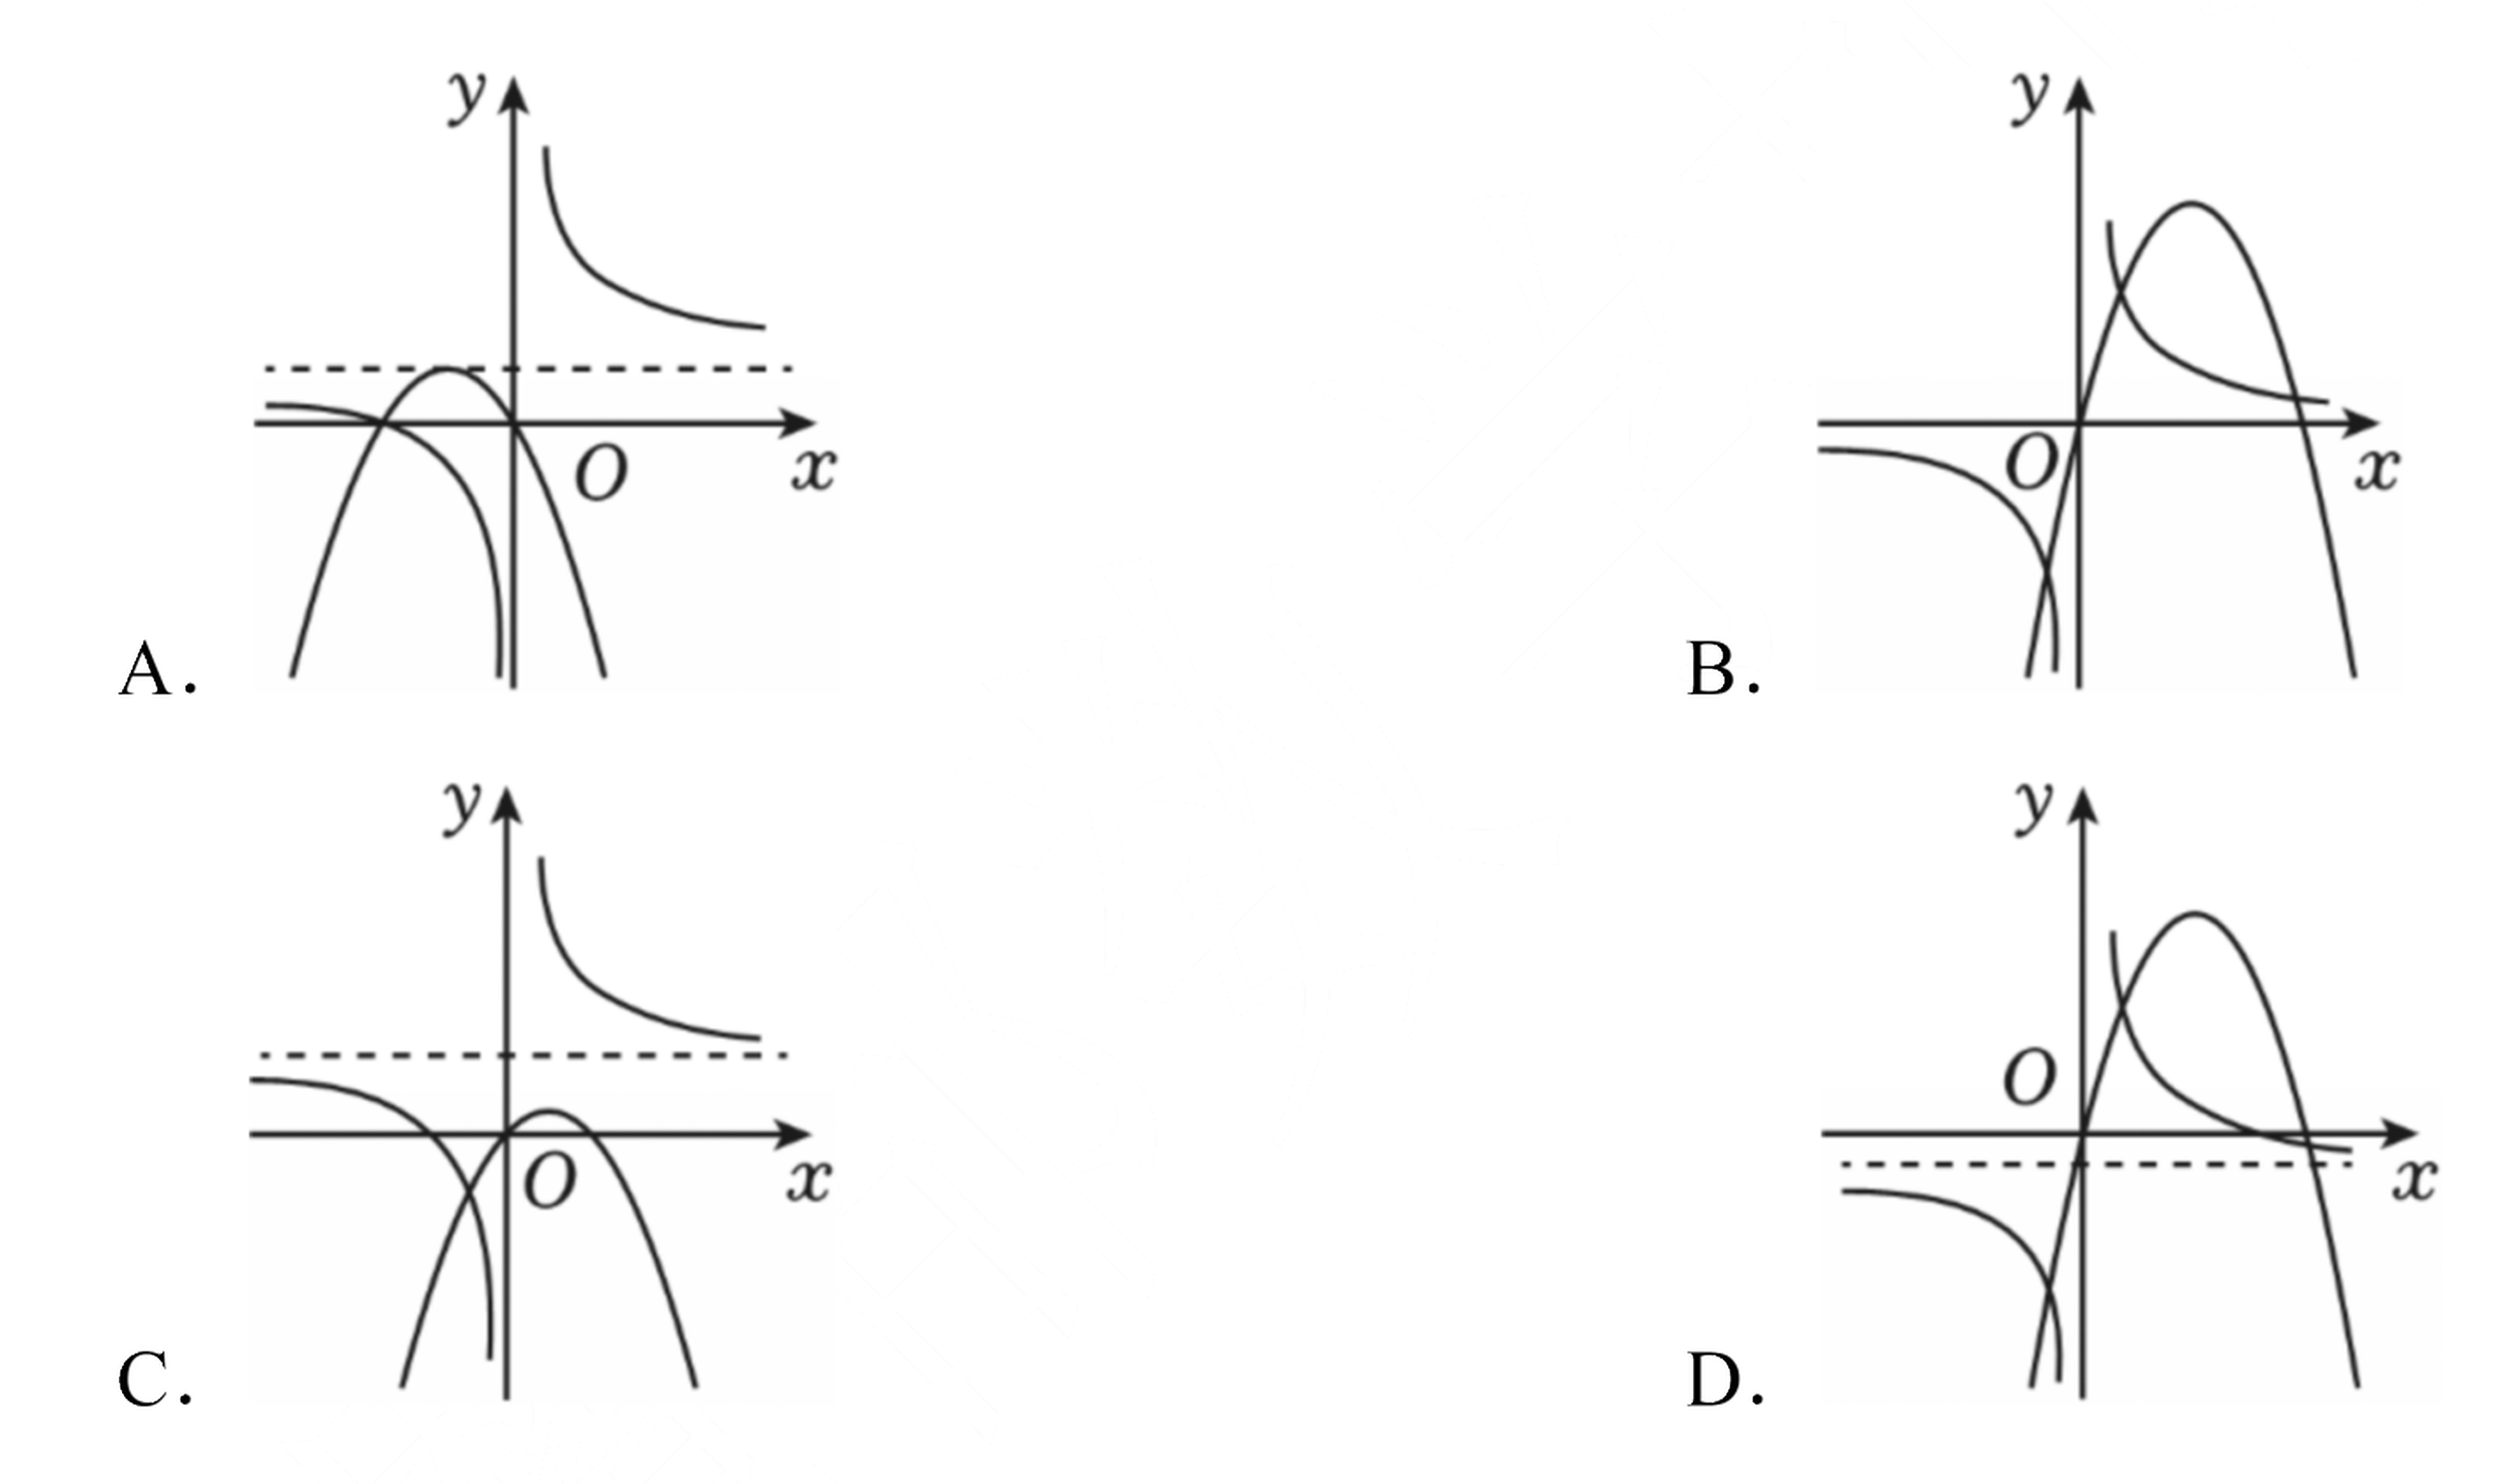
\includegraphics[width=0.80\textwidth]{figures/gao161_q14.png}
\end{center}

\ifanswer
\solbegin
\step{$A$ 选项，由二次函数图象得 $a<0$，$b<0$，由幂函数型函数图象得 $a<0$，$b>0$，}
\step{故 $A$ 选项错误；}
\step{$B$ 选项，由二次函数图象得 $a<0$，$b>0$，由幂函数型函数图象得 $a<0$，$b=0$，}
\step{故 $B$ 选项错误；}
\step{$C$ 选项，由二次函数图象得 $a<0$，$b>0$，由幂函数型函数图象得 $a<0$，$b>0$，}
\step{故 $C$ 选项正确；}
\step{$D$ 选项，由二次函数图象得 $a<0$，$b>0$，由幂函数型函数图象得 $a<0$，$b<0$，}
\step{故 $D$ 选项错误.}
\step{故选 $C$.}
\solend
\fi

% === Q15 === \subseteq／\subset、\varnothing、\mid；"排除 C""排除 B、D"正体字母照录；解析 4 行，故选 $A$
\item 设不等式 $\lvert f(x)\rvert+\lvert g(x)\rvert<a$（常数 $a>0$）的解集是 $M$，设不等式 $\lvert f(x)+g(x)\rvert<a$（常数 $a>0$）的解集是 $N$，则\mbox{（\quad）}

\keepwithprev
A. $M\subseteq N$\qquad B. $N\subseteq M$\qquad C. $M\subset N$\qquad D. $N\subset M$

\ifanswer
\solbegin
\step{$x\in M\Rightarrow\lvert f(x)+g(x)\rvert\leqslant\lvert f(x)\rvert+\lvert g(x)\rvert<a\Rightarrow x\in N$，所以 $M\subseteq N$.}
\step{取 $f(x)=g(x)=0$，则 $M=N$，排除 C.}
\step{取 $f(x)=1$，$g(x)=-1$，$a=1$，则 $M=\varnothing$，$N$ 为全体实数，排除 B、D.}
\step{故选 $A$.}
\solend
\fi

% === Q16 === "人文集"定义证明；cases 无；解析 21 行，故选 $B$
\item 设集合 $I_n=\{1,2,\cdots,n\}$，$n\in\N,n\geqslant1$，集合 $P_n=\left\{\dfrac{m}{\sqrt k}\mid m\in I_n,k\in I_n\right\}$，若 $P_n$ 的子集 $A$ 中任意两个元素之和不是整数的平方，则称 $A$ 为 “人文集”. 那么使 $P_n$ 能分成两个交集为空集的 “人文集” 的并集，且这两个人文集的并集恰为 $P_n$ 时，$n$ 的最大值是\mbox{（\quad）}

\keepwithprev
A. 13\qquad B. 14\qquad C. 15\qquad D. 16

\ifanswer
\solbegin
\step{先证当 $n\geqslant15$ 时，$P_n$ 不能分成两个不相交的人文集的并集.}
\step{假设当 $n\geqslant15$ 时，$P_n$ 可以分成两个不相交的人文集的并集，}
\step{设 $A$ 和 $B$ 为两个不相交的人文集，使 $A\cup B=P_n\supseteq I_n$.}
\step{不妨设 $1\in A$，则由于 $1+3=2^2$，所以 $3\notin A$，即 $3\in B$.}
\step{同理可得，$6\in A$，$10\in B$. 又推出 $15\in A$，}
\step{但 $1+15=4^2$，这与 $A$ 为人文集相矛盾.}
\step{再证 $P_{14}$ 满足要求. 当 $k=1$ 时，$P_{14}=\left\{\dfrac{m}{\sqrt k}\mid m\in I_{14},k\in I_{14}\right\}$，}
\step{可以分成 2 个人文集的并集.}
\step{事实上，只要取 $A_1=\{1,2,4,6,9,11,13\}$，$B_1=\{3,5,7,8,10,12,14\}$，}
\step{则 $A_1$ 和 $B_1$ 都是人文集，且 $A_1\cup B_1=P_{14}$.}
\step{当 $k=4$ 时，集合 $\left\{\dfrac{m}{\sqrt k}\mid m\in I_{14}\right\}$ 中，除整数外，}
\step{剩下的数组成集合 $\left\{\dfrac12,\dfrac32,\dfrac52,\cdots,\dfrac{13}{2}\right\}$，}
\step{可以分为下列 2 个人文集的并：$A_2=\left\{\dfrac12,\dfrac52,\dfrac92,\dfrac{11}{2}\right\}$，$B_2=\left\{\dfrac32,\dfrac72,\dfrac{13}{2}\right\}$.}
\step{当 $k=9$ 时，集合 $\left\{\dfrac{m}{\sqrt k}\mid m\in I_{14}\right\}$ 中，除整数外，}
\step{剩下的数组成集合 $\left\{\dfrac13,\dfrac23,\dfrac43,\dfrac53,\cdots,\dfrac{13}{3},\dfrac{14}{3}\right\}$，}
\step{可以分为下列 2 个人文集的并：$A_3=\left\{\dfrac13,\dfrac43,\dfrac53,\dfrac{10}{3},\dfrac{13}{3}\right\}$，$B_3=\left\{\dfrac23,\dfrac73,\dfrac83,\dfrac{11}{3},\dfrac{14}{3}\right\}$.}
\step{最后，集合 $C=\left\{\dfrac{m}{\sqrt k}\mid m\in I_{14},k\in I_{14},k\ne1,4,9\right\}$ 中的数的分母都是无理数，}
\step{它与 $P_n$ 中的任何其他数之和都不是整数，}
\step{因此，令 $A=A_1\cup A_2\cup A_3\cup C$，$B=B_1\cup B_2\cup B_3$，}
\step{则 $A$ 和 $B$ 是不相交的人文集，且 $A\cup B=P_{14}$.}
\step{综上，$n$ 的最大值为 14，故选 $B$.}
\solend
\fi

\end{enumerate}

\bigsec{三、解答题}

\begin{enumerate}
\setcounter{enumi}{16}

% === Q17 === "图像"照录；\Z；cases 块；解析 9 行，跨 06—07 页
\item (1) 已知函数 $y=x^{\frac{4m-m^2}{2}}$（$m\in\Z$）在区间 $(0,+\infty)$ 上是严格增函数，它的图像关于 $y$ 轴对称，求 $m$ 的值及该函数的解析式；

(2) 若 $(a-2)^{\frac32}<(1+2a)^{\frac32}$，求实数 $a$ 的取值范围.

\ifanswer
\solbegin
\step{(1) 由幂函数在 $(0,+\infty)$ 上严格递增，得 $\dfrac{4m-m^2}{2}>0\Leftrightarrow0<m<4$，}
\step{又 $m\in\Z$，所以 $m\in\{1,2,3\}$.}
\step{当 $m=1$ 或 $m=3$ 时，函数为 $y=x^{\frac32}$，定义域为 $[0,+\infty)$，}
\step{图像不关于 $y$ 轴对称.}
\step{当 $m=2$ 时，函数为 $y=x^2$，满足题意，所以 $m=2$，解析式 $y=x^2$.}
\step{(2) 原不等式有意义，须满足 $\begin{cases}a-2\geqslant0\\1+2a\geqslant0\end{cases}\Leftrightarrow a\geqslant2$，}
\step{函数 $y=x^{\frac32}$ 在 $[0,+\infty)$ 上严格递增，}
\step{因此 $(a-2)^{\frac32}<(1+2a)^{\frac32}\Leftrightarrow a-2<1+2a\Leftrightarrow a>-3$，}
\step{结合 $a\geqslant2$，得 $a\in[2,+\infty)$.}
\solend
\fi

% === Q18 === 题干"$a\geqslant0$"与解析"$a<0$"自相矛盾照录；"$A\cap B=(-2,-1]\cap[2,6)$"误印 ∩ 照录；\subseteq；解析 10 行
\item 已知实数 $a\geqslant0$，集合 $A=\left\{x\mid\dfrac{x+2}{x-6}<0\right\}$，$B=\{x\mid\lvert2x-1\rvert\geqslant3\}$，$C=\{x\mid x^2-3ax+2a^2<0\}$，

(1) 求 $A\cap B$；

(2) 若 $C\subseteq(A\cap B)$，求 $a$ 的取值范围.

\ifanswer
\solbegin
\step{(1) 由 $\dfrac{x+2}{x-6}<0$ 得 $-2<x<6$，即 $A=\{x\mid-2<x<6\}=(-2,6)$，}
\step{由 $\lvert2x-1\rvert\geqslant3$ 得 $2x-1\geqslant3$ 或 $2x-1\leqslant-3$，解得 $x\geqslant2$ 或 $x\leqslant-1$，}
\step{即 $B=(-\infty,-1]\cup[2,+\infty)$，}
\step{所以 $A\cap B=(-2,-1]\cap[2,6)$；}% 原卷把 ∪ 误印成 ∩，照录未改（见 ⑤ 2）
\step{(2) 由 (1) 得 $A\cap B=\{x\mid-2<x\leqslant-1\text{ 或 }2\leqslant x<6\}$，}
\step{因为 $C\subseteq(A\cap B)$，$x^2-3ax+2a^2=(x-a)(x-2a)<0$，}% 题干 $a\geqslant0$ 与解析 $a<0$ 自相矛盾，照录未改（见 ⑤ 1）
\step{当 $a=0$ 时，$C=\varnothing$，符合题意；}
\step{当 $a>0$ 时，$C=(a,2a)$，则 $\begin{cases}a\geqslant2\\2a\leqslant6\\a>0\end{cases}$，解得 $2\leqslant a\leqslant3$，}
\step{当 $a<0$ 时，$C=(2a,a)$，则 $\begin{cases}2a\geqslant-2\\a\leqslant-1\\a<0\end{cases}$，解得 $a=-1$，}
\step{故 $a$ 的范围为 $\{-1,0\}\cup[2,3]$.}
\solend
\fi

% === Q19 === 双碳太阳能应用题；"双碳""自发自用、市电互补"弯引号；解析 8 行，跨 08 页上下
\item 为响应 “双碳” 目标，某电子企业拟安装一套可使用 10 年的太阳能供电设备. 该设备的安装费用 $P(x)$（单位：万元）与太阳能电池板面积 $x(x>0)$（单位：平方米）成正比，比例系数为 $\dfrac12$. 为保障生产用电，安装后采用 “自发自用、市电互补” 模式，在此模式下，企业每年消耗的电费 $Q(x)$（单位：万元）与安装的这种太阳能电池板的面积 $x$ 之间的函数关系是 $Q(x)=\dfrac{180}{x+5}$. 记 $W(x)$（单位：万元）为该企业安装这种太阳能供电设备的费用与 10 年所消耗的电费之和.

(1) 要使该设备的安装费与第 1 年的电费之和不超过 17 万元，求安装太阳能电池板面积 $x$ 的取值范围；

(2) 当 $x$ 为多少平方米时，$W(x)$ 取得最小值？最小值是多少万元？

\ifanswer
\solbegin
\step{(1) $P(x)=\dfrac{x}{2}$，安装费与第 1 年的电费之和不超过 17 万元，即 $\dfrac{x}{2}+\dfrac{180}{x+5}\leqslant17$，}
\step{$x>0$，上式等价于 $x^2-29x+190\leqslant0\Leftrightarrow(x-10)(x-19)\leqslant0$，}
\step{解得 $x\in[10,19]$.}
\step{(2) 安装费用与 10 年电费之和为 $W(x)=P(x)+10Q(x)$，}
\step{$=\dfrac{x}{2}+\dfrac{1800}{x+5}=\dfrac{x+5}{2}+\dfrac{1800}{x+5}-\dfrac52$，}
\step{$x>0$，由基本不等式得 $W(x)\geqslant2\sqrt{\dfrac{x+5}{2}\cdot\dfrac{1800}{x+5}}-\dfrac52=60-\dfrac52=57.5$，}
\step{等号当且仅当 $\dfrac{x+5}{2}=\dfrac{1800}{x+5}$，即 $x=55$ 时成立.}
\step{因此，当电池板面积为 55 平方米时，$W(x)$ 取得最小值 57.5 万元.}
\solend
\fi

% === Q20 === $a*b$ 定义；\min 改正体；cases 块；解析 23 行，跨 08—10 页
\item 设 $a$、$b\in\R$，定义 $a*b=\begin{cases}a,&a<b\\b,&a\geqslant b\end{cases}$.

(1) 若 $x*2>1$，求 $x$ 的取值范围；

(2) 若 $(\lvert x-1\rvert+\lvert x-2\rvert)*3=3$，求 $x$ 的取值范围；

(3) 若 $a$、$b>0$，记 $M=a*\dfrac{b}{a^2+4b^2}$，分别比较 $M$ 与 $a$，以及 $M$ 与 $\dfrac{b}{a^2+4b^2}$ 的大小，并求 $M$ 的最大值.

\ifanswer
\solbegin
\step{(1) 定义 $a*b=\begin{cases}a,&a<b\\b,&a\geqslant b\end{cases}$，由 $x*2>1$，得 $\begin{cases}x<2\\x>1\end{cases}$，或 $\begin{cases}x\geqslant2\\2>1\end{cases}$，}
\step{解得 $x>1$，即 $x$ 的取值范围为 $\{x\mid x>1\}$；}
\step{(2) 当 $x\geqslant2$ 时，$\lvert x-1\rvert+\lvert x-2\rvert=2x-3\geqslant1$，}
\step{当 $1\leqslant2x-3\leqslant3$，即 $2\leqslant x\leqslant3$ 时，}
\step{此时 $(\lvert x-1\rvert+\lvert x-2\rvert)*3=2x-3=3$，解得 $x=3$；}
\step{当 $2x-3>3$，即 $x>3$ 时，}
\step{此时 $(\lvert x-1\rvert+\lvert x-2\rvert)*3=3$ 恒成立，则 $x>3$；}
\step{当 $-2x+3>3$，即 $x<0$ 时，}
\step{此时 $(\lvert x-1\rvert+\lvert x-2\rvert)*3=3$ 恒成立，则 $x<0$.}
\step{当 $1<x<2$ 时，$\lvert x-1\rvert+\lvert x-2\rvert=1$，}
\step{此时 $(\lvert x-1\rvert+\lvert x-2\rvert)*3=1\ne3$，不符合题意；}
\step{当 $x\leqslant1$ 时，$\lvert x-1\rvert+\lvert x-2\rvert=-2x+3\geqslant1$，}
\step{当 $-2x+3\leqslant3$，即 $0\leqslant x\leqslant1$ 时，}
\step{此时 $(\lvert x-1\rvert+\lvert x-2\rvert)*3=-2x+3=3$，解得 $x=0$.}
\step{综上所述，$x$ 的取值范围为 $\{x\mid x\leqslant0\text{ 或 }x\geqslant3\}$；}
\step{(3) 由题意，$M=a*\dfrac{b}{a^2+4b^2}=\min\left\{a,\dfrac{b}{a^2+4b^2}\right\}$，}% 原卷印斜体 min，按全稿惯例改正体 \min（见 ② ⑬）
\step{则 $M\leqslant a$，$M\leqslant\dfrac{b}{a^2+4b^2}$.}
\step{因为 $a$、$b>0$，所以 $\dfrac{b}{a^2+4b^2}\leqslant\dfrac{b}{2\sqrt{a^2\cdot4b^2}}=\dfrac{1}{4a}$，}
\step{当且仅当 $a=2b>0$ 时取等号，}
\step{当 $a\geqslant\dfrac{1}{4a}$，即 $a\geqslant\dfrac12$ 时，$M=a*\dfrac{b}{a^2+4b^2}=\dfrac{b}{a^2+4b^2}\leqslant\dfrac{1}{4a}$，}
\step{则 $a=\dfrac12$，$b=\dfrac14$ 时，$M$ 取得最大值 $\dfrac12$；}
\step{当 $0<a<\dfrac12$ 时，$M=a*\dfrac{b}{a^2+4b^2}=a$，此时 $M<\dfrac12$.}
\step{综上所述，$M$ 的最大值为 $\dfrac12$.}
\solend
\fi

% === Q21 === $A_n$／$B_n$／$S_n$／$T_n$ 新定义；题干第 3 问误标 (2) 照录、解析作 (3)；\prec；解析 25 行，跨 10—11 页
\item 对任意正整数 $n$，记集合 $A_n=\{(a_1,a_2,\cdots,a_n)\mid a_1,a_2,\cdots,a_n$ 均为非负整数，且 $a_1+a_2+\cdots+a_n=n\}$，集合 $B_n=\{(b_1,b_2,\cdots,b_n)\mid b_1,b_2,\cdots,b_n$ 均为非负整数，且 $b_1+b_2+\cdots+b_n=2n\}$. 设 $\alpha=(a_1,a_2,\cdots,a_n)\in A_n$，$\beta=(b_1,b_2,\cdots,b_n)\in B_n$，若对任意 $i\in\{1,2,\cdots,n\}$ 都有 $a_i\leqslant b_i$，则记 $\alpha\prec\beta$.

(1) 写出集合 $A_2$ 和 $B_2$；

(2) 证明：对任意 $\alpha\in A_n$，存在 $\beta\in B_n$，使得 $\alpha\prec\beta$；

(2) 设集合 $S_n=\{(\alpha,\beta)\mid\alpha\in A_n,\beta\in B_n,\alpha\prec\beta\}$，求证：$S_n$ 中的元素个数是完全平方数.% 原卷第 3 问题干误标 (2)（与第 2 问重号），照录未改（见 ⑤ 3）

\ifanswer
\solbegin
\step{(1) $A_2=\{(0,2),(1,1),(2,0)\}$，$B_2=\{(0,4),(1,3),(2,2),(3,1),(4,0)\}$；}
\step{(2) 对任意 $\alpha=(a_1,a_2,\cdots,a_n)\in A_n$，设 $b_i=a_i+1$（$i=1,2,3,\cdots,n$），}
\step{则 $b_1,b_2,\cdots,b_n$ 均为非负整数，且 $a_i\leqslant b_i$（$i=1,2,3,\cdots,n$）.}
\step{令 $\beta=(b_1,b_2,\cdots,b_n)$，则 $b_1+b_2+\cdots+b_n$}
\step{$=(a_1+1)+(a_2+1)+\cdots+(a_n+1)=(a_1+a_2+\cdots+a_n)+n=2n$，}
\step{所以 $\beta\in B_n$，且 $\alpha\prec\beta$.}
\step{(3) 对任意 $\alpha=(a_1,a_2,\cdots,a_n)\in A_n$，$\alpha'=(a_1',a_2',\cdots,a_n')\in A_n$，}
\step{记 $\alpha+\alpha'=(a_1+a_1',a_2+a_2',\cdots,a_n+a_n')$，}
\step{则 $a_1+a_1',a_2+a_2',\cdots,a_n+a_n'$ 均为非负整数，}
\step{且 $(a_1+a_1')+(a_2+a_2')+\cdots+(a_n+a_n')$}
\step{$=(a_1+a_2+\cdots+a_n)+(a_1'+a_2'+\cdots+a_n')=n+n=2n$，}
\step{所以 $\alpha+\alpha'\in B_n$，且 $\alpha\prec\alpha+\alpha'$，$\alpha'\prec\alpha+\alpha'$.}
\step{设集合 $A_n$ 中的元素个数为 $t$，设 $A_n=\{\alpha_1,\alpha_2,\cdots,\alpha_t\}$.}
\step{设集合 $T_n=\{(\alpha_i,\alpha_i+\alpha_j)\mid i=1,2,\cdots,t,j=1,2,\cdots,t\}$.}
\step{对任意 $\alpha_i\in A_n$（$i=1,2,\cdots,t$），都有 $\alpha_i+\alpha_1,\alpha_i+\alpha_2,\cdots,\alpha_i+\alpha_t\in B_n$，}
\step{且 $\alpha_i\prec\alpha_i+\alpha_j$，$j=1,2,\cdots,t$，所以 $T_n\subseteq S_n$.}
\step{若 $(\alpha,\beta)\in S_n$，其中 $\alpha=(a_1,a_2,\cdots,a_n)\in A_n$，$\beta=(b_1,b_2,\cdots,b_n)\in B_n$，}
\step{设 $c_i=b_i-a_i$（$i=1,2,\cdots,n$），因为 $a_i\leqslant b_i$，所以 $c_i=b_i-a_i\geqslant0$，}
\step{记 $\alpha'=(c_1,c_2,\cdots,c_n)$，}
\step{则 $c_1+c_2+\cdots+c_n=(b_1-a_1)+(b_2-a_2)+\cdots+(b_n-a_n)$}
\step{$=(b_1+b_2+\cdots+b_n)-(a_1+a_2+\cdots+a_n)=2n-n=n$，}
\step{所以 $\alpha'\in A_n$，并且有 $\beta=\alpha+\alpha'$，所以 $(\alpha,\beta)\in T_n$，所以 $S_n\subseteq T_n$，}
\step{所以 $S_n=T_n$.}
\step{因为集合 $T_n$ 中的元素个数为 $t^2$，所以 $S_n$ 中的元素个数为 $t^2$，}
\step{是完全平方数.}
\solend
\fi

\end{enumerate}

\end{document}
"
% 紧凑版：xelatex "\def\iscompact{1}% 高一161_松江一中嘉一实验_期中.tex
%   —— 高一上数学"2026-2027 年松江一中嘉一实验高一上期中"（试卷版/答案版/紧凑版）
% 试卷版：xelatex 高一161_松江一中嘉一实验_期中.tex
% 答案版：xelatex "\def\isanswer{1}\input{高一161_松江一中嘉一实验_期中.tex}"
% 紧凑版：xelatex "\def\iscompact{1}\input{高一161_松江一中嘉一实验_期中.tex}"
%
% ① 原始材料：微信公众号"魔都数学加油站"文章，连载"27学年高一161"，原卷卷面标题
% "2026-2027 年松江一中嘉一实验高一上期中"（卷面未印副标题、未印连载号）。
% 正文为 11 张 PNG 页（01/02/03/05/06/07/08/09/11 为 4762×6735，04/10 为
% 2560×3620，同一篇各页分辨率混排，逐页按各自分辨率裁图核对）。
% 体例：讲评版——填空 3—12（10 题）、选择 13—16（4 题）、解答 17—21（5 题），
% 共 19 题，自第 3 题起编（1、2 未印在本篇）；Q13 答案"A"直接印在题干括号内、
% 且无【答案】/【解析】段，本稿按 高一37 第 13 题／高一57 第 13 题成例把括号
% 留空、另提 \ans{$A$}；其余 18 题逐题印【解析】、用 \solbegin…\solend。
% 题目、答案、解析均据原图转录；卷面粉红色水印"魔都数学加油站"及公众号页脚未录入。
% 全卷插图清单（逐页通读 11 页确认）：仅 1 组——Q14 四幅图像选项（04 页 2×2
% 排布，二次函数与幂函数型函数在同一坐标系中的图象，A/B/C/D 四幅小图），
% 合并成一张，三版都出，裁 figures/gao161_q14.png。其余各页逐页确认无其它
% 题目配图、无解析内配图、无表格、无"如图"处（Q16 解析里的"可以分为下列 2 个
% 人文集的并"是纯文字＋集合，不是表格；OCR 里看似表格的行实为大括号与分数）。
%
% 卷首标题：原卷印作"2026-2027 年松江一中嘉一实验高一上期中"，年份区间按全稿惯例排 en dash；
% 原卷卷面未印副标题，本稿按同期中卷知识模块口径补出"集合与常用逻辑用语、不等式、函数"。
%
% ② 与原卷的排版差异／照录项清单：
%   ① 原文从第 3 题起，本稿保留原题号；共 19 题三节，解答题 5 题到 21；
%      三节各自一个 enumerate + \setcounter{enumi}{2}/{12}/{16}（不贯穿），
%      用 \examtitlest[3] 起手；
%   ② 混合体例：Q13 原卷把答案"A"直接印在题干括号内（"（  A  ）"）、且题下
%      无【答案】/【解析】段，按 高一37 第 13 题／高一57 第 13 题成例把括号
%      留空、另提 \ans{$A$}、不补造解析；其余 18 题印【解析】、用
%      \solbegin…\solend；四道选择题中 Q14/Q15/Q16 的答案在解析末句
%      "故选 $C$／$A$／$B$"、Q13 用 \ans{$A$}；括号 \mbox{（\quad）} 留空；
%      答案版【答案】/【解析】标记数 = 19 = 全卷题数（1 个 \ans ＋ 18 个 \solbegin）；
%   ③ 原卷卷面未印副标题，本稿按知识模块口径补出；
%   ④ 原卷填空横线按全稿惯例排 \blankline[4.4em]；选择题选项段前按惯例各加
%      \keepwithprev；Q14 四幅选项图整块用 \needvspace{9cm} 守卫（守卫放
%      \item 之前，见 高一132 Q14／高一154 Q15 成例）；解答题不留作答区、
%      不加 \anspace（原卷为讲评版）；
%   ⑤ 数集归一：Q8"$x\in\R$"、Q11"$m\in\R$"、Q13"$x,y\in\N$"、
%      Q16"$n\in N$"、Q17"$m\in\Z$"、Q20"$a$、$b\in R$"——原卷印正体粗体
%      或斜体 R/N/Z，按全稿惯例归一 \R／\N／\Z；绝对值排 \lvert…\rvert
%      （Q9、Q12、Q15、Q18、Q20），集合描述竖线排 \mid（Q12、Q16、Q18、
%      Q20、Q21），空集 \varnothing（Q15、Q18），补集无用例，不等号按全稿
%      惯例排 \leqslant／\geqslant；
%   ⑥ 子集符号逐处照录不统一：Q12 cases 定义"$C(A)\geqslant C(B)$"、
%      Q15 选项 A/B"$M\subseteq N$""$N\subseteq M$"与解析"$M\subseteq N$"
%      印带下划线 ⊆（照录 \subseteq），Q15 选项 C/D"$M\subset N$""$N\subset M$"
%      印单线 ⊂（照录 \subset），Q18 "$C\subseteq(A\cap B)$"、Q21
%      "$T_n\subseteq S_n$""$S_n\subseteq T_n$"均带下划线照录 \subseteq；
%      本卷无 \not\subset 用例；
%   ⑦ 判别式：Q7 解析"$\Delta=(m-6)(m+2)>0$"、Q8 解析"$\Delta=a^2-4a<0$"、
%      Q12 解析"$\Delta=a^2-8$"共 3 处，逐处放大确认印等腰偏高粗三角
%      （高>宽、右斜边粗），照录 \Delta；本卷无扁等边细线 \triangle 用例；
%   ⑧ 中文弯引号照录：Q7"$m\geqslant6$""有两个不相等的正实数根"及四个
%      条件短语、Q13 反证法命题、Q16"人文集"、Q19"双碳""自发自用、市电互补"；
%      注释里一律 ASCII 引号；数学式内 CJK 用 \text{}（Q18、Q20 解集描述内"或"）；
%   ⑨ "图像／图象"逐处照录不统一：Q4"的图像"、Q17 题干"它的图像关于 $y$ 轴
%      对称"及解析"图像不关于 $y$ 轴对称"印"图像"；Q14 题干"的图象可能为"
%      与解析 A/B/C/D 四行各"由二次函数图象得""由幂函数型函数图象得"
%      共 8 处印"图象"（象，无亻）；
%   ⑩ 文本圈数字逐处照录：Q12 题干①②③④、Q12 解析"故①错误""故②正确"
%      "故③正确""故④错误""故正确的是②③"，均为印刷圈数字（文本模式）；
%   ⑪ 半角逗号在数学组之间是全稿惯例、非笔误，逐处照录（Q5"$a$、$b$"、
%      Q13"$x,y\in\N$"、Q16"$n\in\N,n\geqslant1$"与集合描述内逗号、
%      Q20"$a,b\in\R$"、Q21 各集合描述内逗号）；行末西文句点 ASCII `.`；
%      原卷行中句点（Q16"$10\in B$. 又推出 $15\in A$"、Q16"再证 $P_{14}$
%      满足要求. 当 $k=1$ 时"、Q18"$A\cap B=(-2,-1]\cap[2,6)$；"后的分号）
%      按全稿惯例一律排 ASCII `.`／全角"；"；中文语境行中全角逗号／顿号照录；
%   ⑫ 原卷数学式内联条件（Q14"$y=x^a+b(a\ne0)$"、Q19"$x(x>0)$"、
%      Q11"$\lvert x-m\rvert<n\,(m\in\R,n>0)$"）印半角括号，逐处照录未改
%      全角（同 高一147 口径）；
%      中文语境的括注（Q5"结果用 $a$、$b$ 表示"、Q7"填…"、Q12"填写序号"、
%      Q15"常数 $a>0$"、Q19"单位：万元"）印全角括号，照录；
%   ⑬ 复杂式照录别简化：Q3 $(a^{2-\sqrt3})^{2+\sqrt3}\times\sqrt{a^2}\times
%      b^{\sqrt3}\times b^{1-\sqrt3}$ 与 $a^{(2-\sqrt3)(2+\sqrt3)}\cdot a\cdot
%      b^{\sqrt3+1-\sqrt3}=a\cdot a\cdot b=a^2b$（题干用 \times、解析用 \cdot，
%      逐处照录不统一，见 ⑤）；Q5 $\dfrac{\lg2}{\lg2+\lg3}=\dfrac{a}{a+b}$、
%      Q10 $t-\dfrac3t=2$ 与 $b=a^3$、$ab=a^4=2$、Q11 $\left(2a-\dfrac12
%      -a+\dfrac12,2a-\dfrac12+a-\dfrac12\right)=(a,3a-1)$ 与
%      $\left(\dfrac43,\dfrac53\right]\cup\{2\}$、Q16 各分数集合、Q19
%      $x^2-29x+190\leqslant0$ 与 $W(x)=P(x)+10Q(x)$ 与
%      $2\sqrt{\dfrac{x+5}{2}\cdot\dfrac{1800}{x+5}}-\dfrac52=60-\dfrac52=57.5$、
%      Q20 $M=a*\dfrac{b}{a^2+4b^2}=\min\left\{a,\dfrac{b}{a^2+4b^2}\right\}$
%      与 $\dfrac{b}{2\sqrt{a^2\cdot4b^2}}=\dfrac{1}{4a}$、Q21 各 $A_n$／$B_n$／
%      $T_n$ 定义；\left…\right 不得拆到不同 $…$ 组（Q11 的 \left(…\right)、
%      Q11 的 \left(\dfrac43,\dfrac53\right]、Q16 的 \left\{\dfrac{m}{\sqrt k}
%      \mid…\right\} 与 \left\{\dfrac12,\dfrac32,\dfrac52,\cdots,\dfrac{13}{2}\right\}
%      等、Q20 的 \min\left\{…\right\}）；cases 块整体算一个印刷行
%      （Q12 定义、Q17 (2)、Q18 (2) 两处、Q20 定义与 (1)）；原卷 Q20 解析
%      "$=min\{…\}$"印斜体 min，按 高一122／高一102 成例改正体 \min；
%   ⑭ 一条 \step = 原卷解析的一个印刷行；别并折行、别拆行。跨页续印按题合并
%      （Q6 的 01 页上下题干重复印、Q10 的 01—02 页、Q11 的 02—03 页、
%      Q12 的 03—04 页、Q16 的 05—06 页、Q17 的 06—07 页、Q18 的 07 页
%      上下、Q19 的 08 页上下、Q20 的 08—10 页、Q21 的 10—11 页）；
%      跨半页重叠行（Q10"令 $t=\log_a b>0$…"、Q16"它与 $P_n$ 中的任何
%      其他数之和都不是整数，"、Q18"【解析】(1) 由 $\dfrac{x+2}{x-6}<0$…"、
%      Q19"$x>0$，上式等价于…"、Q20"此时…则 $x<0$."、Q21"若 $(\alpha,\beta)
%      \in S_n$…"与"设 $c_i=b_i-a_i$…"）只算一个印刷行；
%   ⑮ 自定义记号照录：Q12"$C(A)$""$A*B$""$S$"、Q16"$I_n$""$P_n$""人文集"
%      "$A_1$／$B_1$／$A_2$／$B_2$／$A_3$／$B_3$／$C$"、Q20"$a*b$""$M$"、
%      Q21"$A_n$／$B_n$／$S_n$／$T_n$""$\alpha\prec\beta$""$\alpha+\alpha'$"；
%   ⑯ 选项字母体例照录不统一：Q15 解析"排除 C.""排除 B、D."两处原卷印
%      正体（文本模式），Q13 \ans{$A$}、Q14"$A$ 选项"…"故选 $C$"、
%      Q15"故选 $A$"、Q16"故选 $B$"用斜体（数学模式），逐处照录、不统一；
%   ⑰ 红字：全卷逐页扫描无红色加粗小标题（仅粉色水印），故本卷无 \stepm，
%      不引入红色定义；
%
% ③ 行数复核：一条 \step = 原卷解析的一个印刷行，cases 块作一个印刷行计。
%   逐题数（逐页核对定稿）：Q3：1；Q4：1；Q5：1；Q6：3；Q7：4；Q8：4；
%   Q9：2；Q10：2；Q11：7；Q12：8；Q13：0（答案印括号内、提 \ans{}，
%   不计入 \step 账）；Q14：9；Q15：4；Q16：21；Q17：9；Q18：10；Q19：8；
%   Q20：23；Q21：25。
%   合计 142 行（142 条 \step，无 \stepm），与原卷逐题印刷行相等。
%   全卷 19 题：Q13 一处 \ans{} ＋ 其余 18 题设 \solbegin…\solend，
%   答案版【答案】/【解析】标记数 = 19 = 全卷题数。
%
% ④ 页码分布（供回原图复核）：
%   卷首标题＋"一、填空题"＋Q3/Q4/Q5 题干＋解析各 1 行＋Q6 题干首行
%   在 01 页上半；Q6 题干（重复印）＋解析 3 行＋Q7 题干＋解析 4 行在
%   01 页下半；Q8 题干＋解析 4 行＋Q9 题干＋解析 2 行＋Q10 题干＋
%   解析首行在 02 页上半；Q10 解析（重复印）＋末行＋Q11 题干＋解析
%   前 3 行在 02 页下半；Q11 解析后 4 行＋Q12 题干＋cases 定义＋①
%   在 03 页上半；Q12 ②③④ 三命题＋"填写序号"行＋解析前 6 行在
%   03 页下半；Q12 解析后 2 行＋"二、选择题"标题＋Q13 题干＋选项＋
%   Q14 题干＋"（　）"＋A/B 两幅图在 04 页上半；Q14 四幅图（重复印）
%   ＋解析 9 行在 04 页下半；Q15 题干＋选项＋解析 4 行＋Q16 题干＋
%   选项在 05 页上半；Q16 题干（重复印）＋选项＋解析前 10 行在 05 页
%   下半；Q16 解析中 8 行（k=4、k=9 两批＋集合 C＋"它与 $P_n$…"）
%   在 06 页上半；Q16 解析"它与 $P_n$…"（重复印）＋末 3 行＋
%   "三、解答题"标题＋Q17 题干＋两问＋解析前 4 行在 06 页下半；
%   Q17 解析后 5 行＋Q18 题干＋两问＋解析首行在 07 页上半；Q18 解析
%   （重复首行）＋余 9 行在 07 页下半；Q19 题干＋两问＋解析前 2 行在
%   08 页上半；Q19 解析（重复第 2 行）＋余 6 行＋Q20 定义＋(1) 问在
%   08 页下半；Q20 (2)(3) 两问＋解析 (1) 2 行＋(2) 前 7 行在 09 页
%   上半；Q20 解析 (2) 余 4 行＋(3) 前 4 行在 09 页下半；Q20 解析 (3)
%   余 4 行＋Q21 题干＋三问在 10 页上半；Q21 题干（重复印）＋解析
%   (1)(2)(3) 前 8 行在 10 页下半；Q21 解析 (3) 中 10 行在 11 页上半；
%   Q21 解析 (3)（重复 2 行）＋末 7 行"是完全平方数."在 11 页下半。
%   本稿按题连排，不丢行、不并折行；全卷末题为第 21 题，无附加题节。
%
% ⑤ 存疑照录（放大原图确认，照录未改、正文对应处另有 % 注）：
%   1. Q18 题干印"已知实数 $a\geqslant0$"，解析却另设"当 $a<0$ 时"并解出
%      $a=-1$，末行答案"故 $a$ 的范围为 $\{-1,0\}\cup[2,3]$"含负数，
%      与题干 $a\geqslant0$ 自相矛盾——系原卷前后不一，照录未改（放大
%      07 页确认题干确印 $a\geqslant0$）；
%   2. Q18 解析"所以 $A\cap B=(-2,-1]\cap[2,6)$；"原卷把并集误印成
%      交集号 ∩（紧接下一行"$A\cap B=\{x\mid-2<x\leqslant-1$ 或
%      $2\leqslant x<6\}$"用"或"），照录未改（放大 07 页确认印 ∩）；
%   3. Q21 题干第 3 问原卷标号印作"(2)"（与第 2 问重号），而解析里
%      同一问标作"(3)"——原卷笔误，题干与解析逐处照录、不统一；
%   4. Q3 题干四处乘号印"×"（\times）、解析内三处乘号印"·"（\cdot），
%      逐处照录未统一（放大 01 页确认）；
%   5. Q16 解析"先证当 $n\geqslant15$ 时"印 ≥（非 >），与"综上，$n$
%      的最大值为 14"自洽，照录；题干"$n\in N,n\geqslant1$"印斜体
%      $N$、按全稿惯例归一 \N（见 ② ⑤）；
%   6. Q20 解析"$M=a*\dfrac{b}{a^2+4b^2}=min\{…\}$"原卷印斜体 min，
%      按全稿惯例改正体 \min（见 ② ⑬）；末行"$M$ 的最大值为
%      $\dfrac12$"照录；
%   7. Q15 解析"排除 C.""排除 B、D."用正体字母，而"故选 $A$"用斜体
%      字母，原卷体例不一（见 ② ⑯），照录未统一。
%   全卷除此 7 类外未发现其它笔误／自相矛盾处；Q13 只把答案印在括号内、
%   其余 18 题全部印【解析】。
%

\documentclass[a4paper,11pt]{article}
\usepackage{common}

\begin{document}

\examtitlest[3]{2026--2027 年松江一中嘉一实验高一上期中}{集合与常用逻辑用语、不等式、函数}

\bigsec{一、填空题}

\begin{enumerate}
\setcounter{enumi}{2}

% === Q3 === 题干 \times、解析 \cdot 逐处照录；解析 1 行
\item 设 $a>0$，$b>0$，化简 $(a^{2-\sqrt3})^{2+\sqrt3}\times\sqrt{a^2}\times b^{\sqrt3}\times b^{1-\sqrt3}=$\blankline[4.4em].

\ifanswer
\solbegin
\step{因为 $a>0$，所以 $\sqrt{a^2}=a$，原式 $=a^{(2-\sqrt3)(2+\sqrt3)}\cdot a\cdot b^{\sqrt3+1-\sqrt3}=a\cdot a\cdot b=a^2b$.}
\solend
\fi

% === Q4 === "图像"照录；解析 1 行
\item 若幂函数 $y=x^a$ 的图像经过点 $(5,\sqrt5)$，则此幂函数的表达式为 $y=$\blankline[4.4em].

\ifanswer
\solbegin
\step{$5^a=\sqrt5\Rightarrow a=\dfrac12$，所以 $y=\sqrt x$.}
\solend
\fi

% === Q5 === "结果用 $a$、$b$ 表示"全角括号＋顿号照录；解析 1 行
\item 已知 $\lg2=a$，$10^b=3$，则 $\log_6 2=$\blankline[4.4em]（结果用 $a$、$b$ 表示）.

\ifanswer
\solbegin
\step{$\lg3=b$，$\log_6 2=\dfrac{\lg2}{\lg2+\lg3}=\dfrac{a}{a+b}$.}
\solend
\fi

% === Q6 === 对称中心；解析 3 行，题干跨 01 页上下重复印
\item 若函数 $y=\dfrac{mx-1}{x+n}$ 的对称中心是 $(4,-3)$，则 $m+n=$\blankline[4.4em].

\ifanswer
\solbegin
\step{令 $x=-n+t$（$t\ne0$），则 $y-m=-\dfrac{mn+1}{t}$；}
\step{将 $t$ 换成 $-t$，$y-m$ 变为其相反数，因此对称中心为 $(-n,m)$.}
\step{于是 $n=-4$，$m=-3$，得 $m+n=-7$.}
\solend
\fi

% === Q7 === 充要条件；中文弯引号＋圈选条件；\Delta 高瘦；解析 4 行
\item 已知关于 $x$ 的一元二次方程 $x^2-mx+m+3=0$，则 “$m\geqslant6$” 是该方程 “有两个不相等的正实数根” 的\blankline[4.4em]条件（填 “充分不必要”、“必要不充分”、“充要” 或 “既不充分也不必要”）.

\ifanswer
\solbegin
\step{方程有两个不相等的正实数根}
\step{$\Leftrightarrow m>0$、$m+3>0$ 且 $\Delta=(m-6)(m+2)>0\Leftrightarrow m>6$.}
\step{$m>6\Rightarrow m\geqslant6$，但 $m=6$ 时方程有两个相等的正实数根，}
\step{因此为必要不充分条件.}
\solend
\fi

% === Q8 === \R、\Delta；解析 4 行
\item 对于任意的 $x\in\R$，代数式 $\lg(ax^2+ax+1)$ 都有意义，则实数 $a$ 的取值范围是\blankline[4.4em].

\ifanswer
\solbegin
\step{真数须满足 $ax^2+ax+1>0$ 对任意 $x\in\R$ 恒成立.}
\step{$a=0$ 时成立；}
\step{$a\ne0$ 时，恒成立等价于 $a>0$ 且 $\Delta=a^2-4a<0$，解得 $0<a<4$；}
\step{因此 $a\in[0,4)$.}
\solend
\fi

% === Q9 === 绝对值 \lvert…\rvert；解析 2 行
\item 若不等式 $\lvert x+1\rvert-\lvert x-4\rvert<m$ 的解集为非空集合，则实数 $m$ 的取值范围是\blankline[4.4em].

\ifanswer
\solbegin
\step{$\lvert x+1\rvert-\lvert x-4\rvert\geqslant-\lvert(x+1)-(x-4)\rvert=-5$，当 $x=-1$ 时取等号，}
\step{因此原不等式的解集非空 $\Leftrightarrow m>-5$，所求范围为 $(-5,+\infty)$.}
\solend
\fi

% === Q10 === 换底；$\log_2 a\cdot\log_2 b$；解析 2 行，跨 02 页上下
\item 已知 $a>1$，$b>1$，若 $\log_a b-3\log_b a=2$，且 $ab=2$，则 $\log_2 a\cdot\log_2 b=$\blankline[4.4em].

\ifanswer
\solbegin
\step{令 $t=\log_a b>0$，则 $t-\dfrac{3}{t}=2\Leftrightarrow(t-3)(t+1)=0$，得 $t=3$，}
\step{于是 $b=a^3$，$ab=a^4=2$，得 $\log_2 a=\dfrac14$，$\log_2 b=\dfrac34$，所求为 $\dfrac{3}{16}$.}
\solend
\fi

% === Q11 === 邻域定义；\left(…\right) 不拆组；解析 7 行，跨 02—03 页
\item 对于实数 $m$ 和正数 $n$，称满足不等式 $\lvert x-m\rvert<n\,(m\in\R,n>0)$ 的实数 $x$ 的集合叫做 $m$ 的 $n$ 邻域. 已知 $a>\dfrac12$，若 $2a-\dfrac12$ 的 $a-\dfrac12$ 邻域中恰有 2 个整数，则 $a$ 的取值范围是\blankline[4.4em].

\ifanswer
\solbegin
\step{所求邻域为 $\left(2a-\dfrac12-a+\dfrac12,2a-\dfrac12+a-\dfrac12\right)=(a,3a-1)$.}
\step{当 $\dfrac12<a\leqslant1$ 时至多含 1 个整数；}
\step{当 $a>2$ 时，区间长度 $2a-1>3$，至少含 3 个整数.}
\step{当 $1<a<2$ 时，区间必含 2，恰有两个整数等价于 $3<3a-1\leqslant4$，}
\step{即 $\dfrac43<a\leqslant\dfrac53$.}
\step{当 $a=2$ 时，区间为 $(2,5)$，恰含整数 $3,4$；}
\step{所以 $a\in\left(\dfrac43,\dfrac53\right]\cup\{2\}$.}
\solend
\fi

% === Q12 === $C(A)$／$A*B$ 定义题；①②③④ 文本圈数字；\subseteq／\subset、\Delta、\mid、\varnothing；解析 8 行
\item 用 $C(A)$ 表示非空集合 $A$ 中的元素个数. 对于集合 $A$、$B$，定义

$A*B=\begin{cases}C(A)-C(B),&C(A)\geqslant C(B)\\ C(B)-C(A),&C(A)<C(B)\end{cases}$，若 $A=\{0,1\}$，$B=\{x\mid(x^2-ax)(x^2+ax+2)=0\}$，设实数 $a$ 的所有可能取值组成的集合是 $S$，则下列说法正确的是\blankline[4.4em]（填写序号）.

① $C(B)$ 的可能值为 $2,3,4$

② 若 $A*B=2$，则 $a$ 的取值范围为 $(-\infty,-2\sqrt2)\cup(2\sqrt2,+\infty)$

③ 若 $A*B=1$，则 $C(S)=3$

④ 若 $A*B=0$，则 $a$ 的取值范围为 $(-2\sqrt2,2\sqrt2)$

\ifanswer
\solbegin
\step{$x(x-a)=0$ 的根为 $0,a$，而 $x^2+ax+2$ 在这两处的值分别为 $2,2a^2+2$，}
\step{两个因式无公共实根；后者的判别式为 $\Delta=a^2-8$.}
\step{当 $a=0$、$0<\lvert a\rvert<2\sqrt2$、$\lvert a\rvert=2\sqrt2$、$\lvert a\rvert>2\sqrt2$ 时，$C(B)$ 依次为 $1,2,3,4$，}
\step{故①错误.}
\step{$A*B=\lvert2-C(B)\rvert$，所以 $A*B=2\Leftrightarrow\lvert a\rvert>2\sqrt2$，故②正确；}
\step{$A*B=1\Leftrightarrow a\in\{-2\sqrt2,0,2\sqrt2\}$，此时 $C(S)=3$，故③正确；}
\step{$A*B=0\Leftrightarrow0<\lvert a\rvert<2\sqrt2$，即 $a\in(-2\sqrt2,0)\cup(0,2\sqrt2)$，故④错误.}
\step{故正确的是②③.}
\solend
\fi

\end{enumerate}

\needvspace{7cm}
\bigsec{二、选择题}

\begin{enumerate}
\setcounter{enumi}{12}

% === Q13 === 答案"A"原卷印在题干括号内、题下无【答案】/【解析】段；按 高一37／高一57 成例另提 \ans{}
\item 用反证法证明命题 “已知 $x>0$，$y>0$，$x,y\in\N$，如果 $xy$ 可被 7 整除，那么 $x$，$y$ 至少有一个能被 7 整除” 时，假设的内容是\mbox{（\quad）}

\keepwithprev
A. $x$、$y$ 都不能被 7 整除\qquad B. $x$、$y$ 都能被 7 整除

C. $x$、$y$ 只有一个能被 7 整除\qquad D. 只有 $x$ 不能被 7 整除

\ifanswer
\ans{$A$}
\fi

% === Q14 === 四幅图像选项（2×2 合并，三版都出）；守卫放 \item 之前；"图象"照录；解析 9 行，故选 $C$
\needvspace{9cm}
\item 函数 $y=ax^2+bx$ 与函数 $y=x^a+b(a\ne0)$ 在同一平面直角坐标系中的图象可能为\mbox{（\quad）}

\keepwithprev
\begin{center}
% 四幅图象选项取 04 页 2×2 排布合并为一张，去粉色水印、转灰度、4× LANCZOS 放大；三版都出
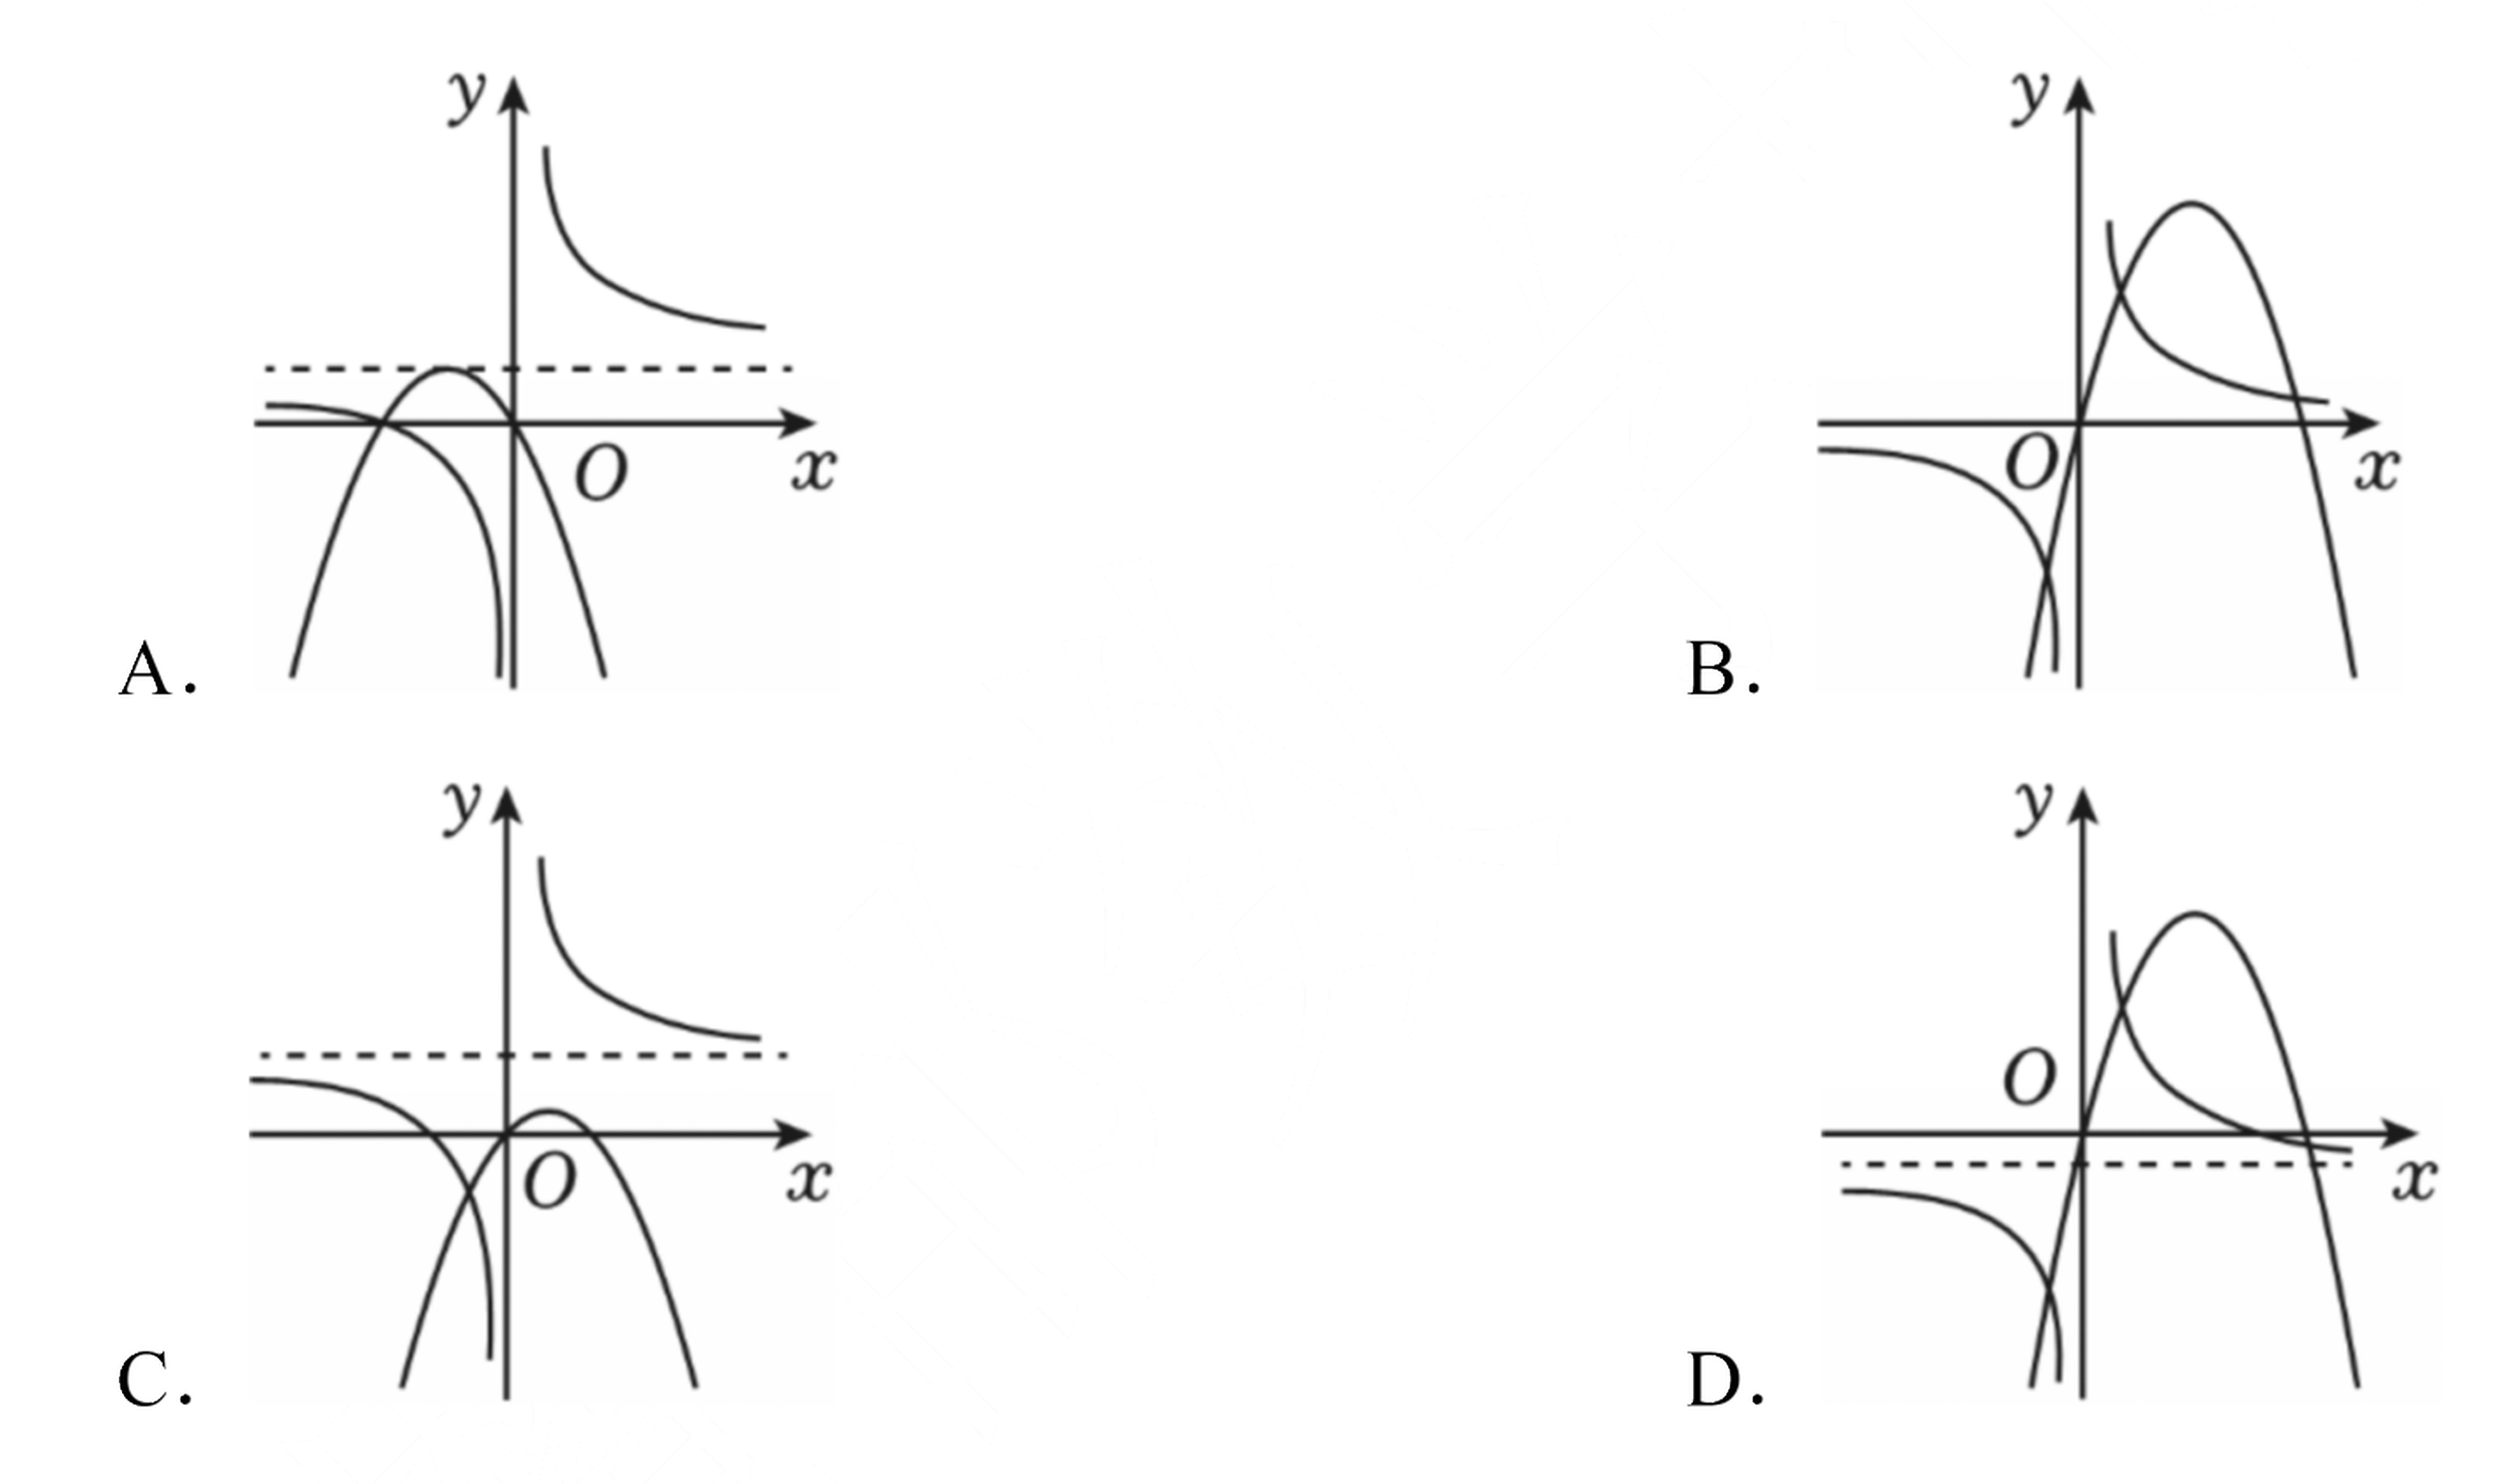
\includegraphics[width=0.80\textwidth]{figures/gao161_q14.png}
\end{center}

\ifanswer
\solbegin
\step{$A$ 选项，由二次函数图象得 $a<0$，$b<0$，由幂函数型函数图象得 $a<0$，$b>0$，}
\step{故 $A$ 选项错误；}
\step{$B$ 选项，由二次函数图象得 $a<0$，$b>0$，由幂函数型函数图象得 $a<0$，$b=0$，}
\step{故 $B$ 选项错误；}
\step{$C$ 选项，由二次函数图象得 $a<0$，$b>0$，由幂函数型函数图象得 $a<0$，$b>0$，}
\step{故 $C$ 选项正确；}
\step{$D$ 选项，由二次函数图象得 $a<0$，$b>0$，由幂函数型函数图象得 $a<0$，$b<0$，}
\step{故 $D$ 选项错误.}
\step{故选 $C$.}
\solend
\fi

% === Q15 === \subseteq／\subset、\varnothing、\mid；"排除 C""排除 B、D"正体字母照录；解析 4 行，故选 $A$
\item 设不等式 $\lvert f(x)\rvert+\lvert g(x)\rvert<a$（常数 $a>0$）的解集是 $M$，设不等式 $\lvert f(x)+g(x)\rvert<a$（常数 $a>0$）的解集是 $N$，则\mbox{（\quad）}

\keepwithprev
A. $M\subseteq N$\qquad B. $N\subseteq M$\qquad C. $M\subset N$\qquad D. $N\subset M$

\ifanswer
\solbegin
\step{$x\in M\Rightarrow\lvert f(x)+g(x)\rvert\leqslant\lvert f(x)\rvert+\lvert g(x)\rvert<a\Rightarrow x\in N$，所以 $M\subseteq N$.}
\step{取 $f(x)=g(x)=0$，则 $M=N$，排除 C.}
\step{取 $f(x)=1$，$g(x)=-1$，$a=1$，则 $M=\varnothing$，$N$ 为全体实数，排除 B、D.}
\step{故选 $A$.}
\solend
\fi

% === Q16 === "人文集"定义证明；cases 无；解析 21 行，故选 $B$
\item 设集合 $I_n=\{1,2,\cdots,n\}$，$n\in\N,n\geqslant1$，集合 $P_n=\left\{\dfrac{m}{\sqrt k}\mid m\in I_n,k\in I_n\right\}$，若 $P_n$ 的子集 $A$ 中任意两个元素之和不是整数的平方，则称 $A$ 为 “人文集”. 那么使 $P_n$ 能分成两个交集为空集的 “人文集” 的并集，且这两个人文集的并集恰为 $P_n$ 时，$n$ 的最大值是\mbox{（\quad）}

\keepwithprev
A. 13\qquad B. 14\qquad C. 15\qquad D. 16

\ifanswer
\solbegin
\step{先证当 $n\geqslant15$ 时，$P_n$ 不能分成两个不相交的人文集的并集.}
\step{假设当 $n\geqslant15$ 时，$P_n$ 可以分成两个不相交的人文集的并集，}
\step{设 $A$ 和 $B$ 为两个不相交的人文集，使 $A\cup B=P_n\supseteq I_n$.}
\step{不妨设 $1\in A$，则由于 $1+3=2^2$，所以 $3\notin A$，即 $3\in B$.}
\step{同理可得，$6\in A$，$10\in B$. 又推出 $15\in A$，}
\step{但 $1+15=4^2$，这与 $A$ 为人文集相矛盾.}
\step{再证 $P_{14}$ 满足要求. 当 $k=1$ 时，$P_{14}=\left\{\dfrac{m}{\sqrt k}\mid m\in I_{14},k\in I_{14}\right\}$，}
\step{可以分成 2 个人文集的并集.}
\step{事实上，只要取 $A_1=\{1,2,4,6,9,11,13\}$，$B_1=\{3,5,7,8,10,12,14\}$，}
\step{则 $A_1$ 和 $B_1$ 都是人文集，且 $A_1\cup B_1=P_{14}$.}
\step{当 $k=4$ 时，集合 $\left\{\dfrac{m}{\sqrt k}\mid m\in I_{14}\right\}$ 中，除整数外，}
\step{剩下的数组成集合 $\left\{\dfrac12,\dfrac32,\dfrac52,\cdots,\dfrac{13}{2}\right\}$，}
\step{可以分为下列 2 个人文集的并：$A_2=\left\{\dfrac12,\dfrac52,\dfrac92,\dfrac{11}{2}\right\}$，$B_2=\left\{\dfrac32,\dfrac72,\dfrac{13}{2}\right\}$.}
\step{当 $k=9$ 时，集合 $\left\{\dfrac{m}{\sqrt k}\mid m\in I_{14}\right\}$ 中，除整数外，}
\step{剩下的数组成集合 $\left\{\dfrac13,\dfrac23,\dfrac43,\dfrac53,\cdots,\dfrac{13}{3},\dfrac{14}{3}\right\}$，}
\step{可以分为下列 2 个人文集的并：$A_3=\left\{\dfrac13,\dfrac43,\dfrac53,\dfrac{10}{3},\dfrac{13}{3}\right\}$，$B_3=\left\{\dfrac23,\dfrac73,\dfrac83,\dfrac{11}{3},\dfrac{14}{3}\right\}$.}
\step{最后，集合 $C=\left\{\dfrac{m}{\sqrt k}\mid m\in I_{14},k\in I_{14},k\ne1,4,9\right\}$ 中的数的分母都是无理数，}
\step{它与 $P_n$ 中的任何其他数之和都不是整数，}
\step{因此，令 $A=A_1\cup A_2\cup A_3\cup C$，$B=B_1\cup B_2\cup B_3$，}
\step{则 $A$ 和 $B$ 是不相交的人文集，且 $A\cup B=P_{14}$.}
\step{综上，$n$ 的最大值为 14，故选 $B$.}
\solend
\fi

\end{enumerate}

\bigsec{三、解答题}

\begin{enumerate}
\setcounter{enumi}{16}

% === Q17 === "图像"照录；\Z；cases 块；解析 9 行，跨 06—07 页
\item (1) 已知函数 $y=x^{\frac{4m-m^2}{2}}$（$m\in\Z$）在区间 $(0,+\infty)$ 上是严格增函数，它的图像关于 $y$ 轴对称，求 $m$ 的值及该函数的解析式；

(2) 若 $(a-2)^{\frac32}<(1+2a)^{\frac32}$，求实数 $a$ 的取值范围.

\ifanswer
\solbegin
\step{(1) 由幂函数在 $(0,+\infty)$ 上严格递增，得 $\dfrac{4m-m^2}{2}>0\Leftrightarrow0<m<4$，}
\step{又 $m\in\Z$，所以 $m\in\{1,2,3\}$.}
\step{当 $m=1$ 或 $m=3$ 时，函数为 $y=x^{\frac32}$，定义域为 $[0,+\infty)$，}
\step{图像不关于 $y$ 轴对称.}
\step{当 $m=2$ 时，函数为 $y=x^2$，满足题意，所以 $m=2$，解析式 $y=x^2$.}
\step{(2) 原不等式有意义，须满足 $\begin{cases}a-2\geqslant0\\1+2a\geqslant0\end{cases}\Leftrightarrow a\geqslant2$，}
\step{函数 $y=x^{\frac32}$ 在 $[0,+\infty)$ 上严格递增，}
\step{因此 $(a-2)^{\frac32}<(1+2a)^{\frac32}\Leftrightarrow a-2<1+2a\Leftrightarrow a>-3$，}
\step{结合 $a\geqslant2$，得 $a\in[2,+\infty)$.}
\solend
\fi

% === Q18 === 题干"$a\geqslant0$"与解析"$a<0$"自相矛盾照录；"$A\cap B=(-2,-1]\cap[2,6)$"误印 ∩ 照录；\subseteq；解析 10 行
\item 已知实数 $a\geqslant0$，集合 $A=\left\{x\mid\dfrac{x+2}{x-6}<0\right\}$，$B=\{x\mid\lvert2x-1\rvert\geqslant3\}$，$C=\{x\mid x^2-3ax+2a^2<0\}$，

(1) 求 $A\cap B$；

(2) 若 $C\subseteq(A\cap B)$，求 $a$ 的取值范围.

\ifanswer
\solbegin
\step{(1) 由 $\dfrac{x+2}{x-6}<0$ 得 $-2<x<6$，即 $A=\{x\mid-2<x<6\}=(-2,6)$，}
\step{由 $\lvert2x-1\rvert\geqslant3$ 得 $2x-1\geqslant3$ 或 $2x-1\leqslant-3$，解得 $x\geqslant2$ 或 $x\leqslant-1$，}
\step{即 $B=(-\infty,-1]\cup[2,+\infty)$，}
\step{所以 $A\cap B=(-2,-1]\cap[2,6)$；}% 原卷把 ∪ 误印成 ∩，照录未改（见 ⑤ 2）
\step{(2) 由 (1) 得 $A\cap B=\{x\mid-2<x\leqslant-1\text{ 或 }2\leqslant x<6\}$，}
\step{因为 $C\subseteq(A\cap B)$，$x^2-3ax+2a^2=(x-a)(x-2a)<0$，}% 题干 $a\geqslant0$ 与解析 $a<0$ 自相矛盾，照录未改（见 ⑤ 1）
\step{当 $a=0$ 时，$C=\varnothing$，符合题意；}
\step{当 $a>0$ 时，$C=(a,2a)$，则 $\begin{cases}a\geqslant2\\2a\leqslant6\\a>0\end{cases}$，解得 $2\leqslant a\leqslant3$，}
\step{当 $a<0$ 时，$C=(2a,a)$，则 $\begin{cases}2a\geqslant-2\\a\leqslant-1\\a<0\end{cases}$，解得 $a=-1$，}
\step{故 $a$ 的范围为 $\{-1,0\}\cup[2,3]$.}
\solend
\fi

% === Q19 === 双碳太阳能应用题；"双碳""自发自用、市电互补"弯引号；解析 8 行，跨 08 页上下
\item 为响应 “双碳” 目标，某电子企业拟安装一套可使用 10 年的太阳能供电设备. 该设备的安装费用 $P(x)$（单位：万元）与太阳能电池板面积 $x(x>0)$（单位：平方米）成正比，比例系数为 $\dfrac12$. 为保障生产用电，安装后采用 “自发自用、市电互补” 模式，在此模式下，企业每年消耗的电费 $Q(x)$（单位：万元）与安装的这种太阳能电池板的面积 $x$ 之间的函数关系是 $Q(x)=\dfrac{180}{x+5}$. 记 $W(x)$（单位：万元）为该企业安装这种太阳能供电设备的费用与 10 年所消耗的电费之和.

(1) 要使该设备的安装费与第 1 年的电费之和不超过 17 万元，求安装太阳能电池板面积 $x$ 的取值范围；

(2) 当 $x$ 为多少平方米时，$W(x)$ 取得最小值？最小值是多少万元？

\ifanswer
\solbegin
\step{(1) $P(x)=\dfrac{x}{2}$，安装费与第 1 年的电费之和不超过 17 万元，即 $\dfrac{x}{2}+\dfrac{180}{x+5}\leqslant17$，}
\step{$x>0$，上式等价于 $x^2-29x+190\leqslant0\Leftrightarrow(x-10)(x-19)\leqslant0$，}
\step{解得 $x\in[10,19]$.}
\step{(2) 安装费用与 10 年电费之和为 $W(x)=P(x)+10Q(x)$，}
\step{$=\dfrac{x}{2}+\dfrac{1800}{x+5}=\dfrac{x+5}{2}+\dfrac{1800}{x+5}-\dfrac52$，}
\step{$x>0$，由基本不等式得 $W(x)\geqslant2\sqrt{\dfrac{x+5}{2}\cdot\dfrac{1800}{x+5}}-\dfrac52=60-\dfrac52=57.5$，}
\step{等号当且仅当 $\dfrac{x+5}{2}=\dfrac{1800}{x+5}$，即 $x=55$ 时成立.}
\step{因此，当电池板面积为 55 平方米时，$W(x)$ 取得最小值 57.5 万元.}
\solend
\fi

% === Q20 === $a*b$ 定义；\min 改正体；cases 块；解析 23 行，跨 08—10 页
\item 设 $a$、$b\in\R$，定义 $a*b=\begin{cases}a,&a<b\\b,&a\geqslant b\end{cases}$.

(1) 若 $x*2>1$，求 $x$ 的取值范围；

(2) 若 $(\lvert x-1\rvert+\lvert x-2\rvert)*3=3$，求 $x$ 的取值范围；

(3) 若 $a$、$b>0$，记 $M=a*\dfrac{b}{a^2+4b^2}$，分别比较 $M$ 与 $a$，以及 $M$ 与 $\dfrac{b}{a^2+4b^2}$ 的大小，并求 $M$ 的最大值.

\ifanswer
\solbegin
\step{(1) 定义 $a*b=\begin{cases}a,&a<b\\b,&a\geqslant b\end{cases}$，由 $x*2>1$，得 $\begin{cases}x<2\\x>1\end{cases}$，或 $\begin{cases}x\geqslant2\\2>1\end{cases}$，}
\step{解得 $x>1$，即 $x$ 的取值范围为 $\{x\mid x>1\}$；}
\step{(2) 当 $x\geqslant2$ 时，$\lvert x-1\rvert+\lvert x-2\rvert=2x-3\geqslant1$，}
\step{当 $1\leqslant2x-3\leqslant3$，即 $2\leqslant x\leqslant3$ 时，}
\step{此时 $(\lvert x-1\rvert+\lvert x-2\rvert)*3=2x-3=3$，解得 $x=3$；}
\step{当 $2x-3>3$，即 $x>3$ 时，}
\step{此时 $(\lvert x-1\rvert+\lvert x-2\rvert)*3=3$ 恒成立，则 $x>3$；}
\step{当 $-2x+3>3$，即 $x<0$ 时，}
\step{此时 $(\lvert x-1\rvert+\lvert x-2\rvert)*3=3$ 恒成立，则 $x<0$.}
\step{当 $1<x<2$ 时，$\lvert x-1\rvert+\lvert x-2\rvert=1$，}
\step{此时 $(\lvert x-1\rvert+\lvert x-2\rvert)*3=1\ne3$，不符合题意；}
\step{当 $x\leqslant1$ 时，$\lvert x-1\rvert+\lvert x-2\rvert=-2x+3\geqslant1$，}
\step{当 $-2x+3\leqslant3$，即 $0\leqslant x\leqslant1$ 时，}
\step{此时 $(\lvert x-1\rvert+\lvert x-2\rvert)*3=-2x+3=3$，解得 $x=0$.}
\step{综上所述，$x$ 的取值范围为 $\{x\mid x\leqslant0\text{ 或 }x\geqslant3\}$；}
\step{(3) 由题意，$M=a*\dfrac{b}{a^2+4b^2}=\min\left\{a,\dfrac{b}{a^2+4b^2}\right\}$，}% 原卷印斜体 min，按全稿惯例改正体 \min（见 ② ⑬）
\step{则 $M\leqslant a$，$M\leqslant\dfrac{b}{a^2+4b^2}$.}
\step{因为 $a$、$b>0$，所以 $\dfrac{b}{a^2+4b^2}\leqslant\dfrac{b}{2\sqrt{a^2\cdot4b^2}}=\dfrac{1}{4a}$，}
\step{当且仅当 $a=2b>0$ 时取等号，}
\step{当 $a\geqslant\dfrac{1}{4a}$，即 $a\geqslant\dfrac12$ 时，$M=a*\dfrac{b}{a^2+4b^2}=\dfrac{b}{a^2+4b^2}\leqslant\dfrac{1}{4a}$，}
\step{则 $a=\dfrac12$，$b=\dfrac14$ 时，$M$ 取得最大值 $\dfrac12$；}
\step{当 $0<a<\dfrac12$ 时，$M=a*\dfrac{b}{a^2+4b^2}=a$，此时 $M<\dfrac12$.}
\step{综上所述，$M$ 的最大值为 $\dfrac12$.}
\solend
\fi

% === Q21 === $A_n$／$B_n$／$S_n$／$T_n$ 新定义；题干第 3 问误标 (2) 照录、解析作 (3)；\prec；解析 25 行，跨 10—11 页
\item 对任意正整数 $n$，记集合 $A_n=\{(a_1,a_2,\cdots,a_n)\mid a_1,a_2,\cdots,a_n$ 均为非负整数，且 $a_1+a_2+\cdots+a_n=n\}$，集合 $B_n=\{(b_1,b_2,\cdots,b_n)\mid b_1,b_2,\cdots,b_n$ 均为非负整数，且 $b_1+b_2+\cdots+b_n=2n\}$. 设 $\alpha=(a_1,a_2,\cdots,a_n)\in A_n$，$\beta=(b_1,b_2,\cdots,b_n)\in B_n$，若对任意 $i\in\{1,2,\cdots,n\}$ 都有 $a_i\leqslant b_i$，则记 $\alpha\prec\beta$.

(1) 写出集合 $A_2$ 和 $B_2$；

(2) 证明：对任意 $\alpha\in A_n$，存在 $\beta\in B_n$，使得 $\alpha\prec\beta$；

(2) 设集合 $S_n=\{(\alpha,\beta)\mid\alpha\in A_n,\beta\in B_n,\alpha\prec\beta\}$，求证：$S_n$ 中的元素个数是完全平方数.% 原卷第 3 问题干误标 (2)（与第 2 问重号），照录未改（见 ⑤ 3）

\ifanswer
\solbegin
\step{(1) $A_2=\{(0,2),(1,1),(2,0)\}$，$B_2=\{(0,4),(1,3),(2,2),(3,1),(4,0)\}$；}
\step{(2) 对任意 $\alpha=(a_1,a_2,\cdots,a_n)\in A_n$，设 $b_i=a_i+1$（$i=1,2,3,\cdots,n$），}
\step{则 $b_1,b_2,\cdots,b_n$ 均为非负整数，且 $a_i\leqslant b_i$（$i=1,2,3,\cdots,n$）.}
\step{令 $\beta=(b_1,b_2,\cdots,b_n)$，则 $b_1+b_2+\cdots+b_n$}
\step{$=(a_1+1)+(a_2+1)+\cdots+(a_n+1)=(a_1+a_2+\cdots+a_n)+n=2n$，}
\step{所以 $\beta\in B_n$，且 $\alpha\prec\beta$.}
\step{(3) 对任意 $\alpha=(a_1,a_2,\cdots,a_n)\in A_n$，$\alpha'=(a_1',a_2',\cdots,a_n')\in A_n$，}
\step{记 $\alpha+\alpha'=(a_1+a_1',a_2+a_2',\cdots,a_n+a_n')$，}
\step{则 $a_1+a_1',a_2+a_2',\cdots,a_n+a_n'$ 均为非负整数，}
\step{且 $(a_1+a_1')+(a_2+a_2')+\cdots+(a_n+a_n')$}
\step{$=(a_1+a_2+\cdots+a_n)+(a_1'+a_2'+\cdots+a_n')=n+n=2n$，}
\step{所以 $\alpha+\alpha'\in B_n$，且 $\alpha\prec\alpha+\alpha'$，$\alpha'\prec\alpha+\alpha'$.}
\step{设集合 $A_n$ 中的元素个数为 $t$，设 $A_n=\{\alpha_1,\alpha_2,\cdots,\alpha_t\}$.}
\step{设集合 $T_n=\{(\alpha_i,\alpha_i+\alpha_j)\mid i=1,2,\cdots,t,j=1,2,\cdots,t\}$.}
\step{对任意 $\alpha_i\in A_n$（$i=1,2,\cdots,t$），都有 $\alpha_i+\alpha_1,\alpha_i+\alpha_2,\cdots,\alpha_i+\alpha_t\in B_n$，}
\step{且 $\alpha_i\prec\alpha_i+\alpha_j$，$j=1,2,\cdots,t$，所以 $T_n\subseteq S_n$.}
\step{若 $(\alpha,\beta)\in S_n$，其中 $\alpha=(a_1,a_2,\cdots,a_n)\in A_n$，$\beta=(b_1,b_2,\cdots,b_n)\in B_n$，}
\step{设 $c_i=b_i-a_i$（$i=1,2,\cdots,n$），因为 $a_i\leqslant b_i$，所以 $c_i=b_i-a_i\geqslant0$，}
\step{记 $\alpha'=(c_1,c_2,\cdots,c_n)$，}
\step{则 $c_1+c_2+\cdots+c_n=(b_1-a_1)+(b_2-a_2)+\cdots+(b_n-a_n)$}
\step{$=(b_1+b_2+\cdots+b_n)-(a_1+a_2+\cdots+a_n)=2n-n=n$，}
\step{所以 $\alpha'\in A_n$，并且有 $\beta=\alpha+\alpha'$，所以 $(\alpha,\beta)\in T_n$，所以 $S_n\subseteq T_n$，}
\step{所以 $S_n=T_n$.}
\step{因为集合 $T_n$ 中的元素个数为 $t^2$，所以 $S_n$ 中的元素个数为 $t^2$，}
\step{是完全平方数.}
\solend
\fi

\end{enumerate}

\end{document}
"
%
% ① 原始材料：微信公众号"魔都数学加油站"文章，连载"27学年高一161"，原卷卷面标题
% "2026-2027 年松江一中嘉一实验高一上期中"（卷面未印副标题、未印连载号）。
% 正文为 11 张 PNG 页（01/02/03/05/06/07/08/09/11 为 4762×6735，04/10 为
% 2560×3620，同一篇各页分辨率混排，逐页按各自分辨率裁图核对）。
% 体例：讲评版——填空 3—12（10 题）、选择 13—16（4 题）、解答 17—21（5 题），
% 共 19 题，自第 3 题起编（1、2 未印在本篇）；Q13 答案"A"直接印在题干括号内、
% 且无【答案】/【解析】段，本稿按 高一37 第 13 题／高一57 第 13 题成例把括号
% 留空、另提 \ans{$A$}；其余 18 题逐题印【解析】、用 \solbegin…\solend。
% 题目、答案、解析均据原图转录；卷面粉红色水印"魔都数学加油站"及公众号页脚未录入。
% 全卷插图清单（逐页通读 11 页确认）：仅 1 组——Q14 四幅图像选项（04 页 2×2
% 排布，二次函数与幂函数型函数在同一坐标系中的图象，A/B/C/D 四幅小图），
% 合并成一张，三版都出，裁 figures/gao161_q14.png。其余各页逐页确认无其它
% 题目配图、无解析内配图、无表格、无"如图"处（Q16 解析里的"可以分为下列 2 个
% 人文集的并"是纯文字＋集合，不是表格；OCR 里看似表格的行实为大括号与分数）。
%
% 卷首标题：原卷印作"2026-2027 年松江一中嘉一实验高一上期中"，年份区间按全稿惯例排 en dash；
% 原卷卷面未印副标题，本稿按同期中卷知识模块口径补出"集合与常用逻辑用语、不等式、函数"。
%
% ② 与原卷的排版差异／照录项清单：
%   ① 原文从第 3 题起，本稿保留原题号；共 19 题三节，解答题 5 题到 21；
%      三节各自一个 enumerate + \setcounter{enumi}{2}/{12}/{16}（不贯穿），
%      用 \examtitlest[3] 起手；
%   ② 混合体例：Q13 原卷把答案"A"直接印在题干括号内（"（  A  ）"）、且题下
%      无【答案】/【解析】段，按 高一37 第 13 题／高一57 第 13 题成例把括号
%      留空、另提 \ans{$A$}、不补造解析；其余 18 题印【解析】、用
%      \solbegin…\solend；四道选择题中 Q14/Q15/Q16 的答案在解析末句
%      "故选 $C$／$A$／$B$"、Q13 用 \ans{$A$}；括号 \mbox{（\quad）} 留空；
%      答案版【答案】/【解析】标记数 = 19 = 全卷题数（1 个 \ans ＋ 18 个 \solbegin）；
%   ③ 原卷卷面未印副标题，本稿按知识模块口径补出；
%   ④ 原卷填空横线按全稿惯例排 \blankline[4.4em]；选择题选项段前按惯例各加
%      \keepwithprev；Q14 四幅选项图整块用 \needvspace{9cm} 守卫（守卫放
%      \item 之前，见 高一132 Q14／高一154 Q15 成例）；解答题不留作答区、
%      不加 \anspace（原卷为讲评版）；
%   ⑤ 数集归一：Q8"$x\in\R$"、Q11"$m\in\R$"、Q13"$x,y\in\N$"、
%      Q16"$n\in N$"、Q17"$m\in\Z$"、Q20"$a$、$b\in R$"——原卷印正体粗体
%      或斜体 R/N/Z，按全稿惯例归一 \R／\N／\Z；绝对值排 \lvert…\rvert
%      （Q9、Q12、Q15、Q18、Q20），集合描述竖线排 \mid（Q12、Q16、Q18、
%      Q20、Q21），空集 \varnothing（Q15、Q18），补集无用例，不等号按全稿
%      惯例排 \leqslant／\geqslant；
%   ⑥ 子集符号逐处照录不统一：Q12 cases 定义"$C(A)\geqslant C(B)$"、
%      Q15 选项 A/B"$M\subseteq N$""$N\subseteq M$"与解析"$M\subseteq N$"
%      印带下划线 ⊆（照录 \subseteq），Q15 选项 C/D"$M\subset N$""$N\subset M$"
%      印单线 ⊂（照录 \subset），Q18 "$C\subseteq(A\cap B)$"、Q21
%      "$T_n\subseteq S_n$""$S_n\subseteq T_n$"均带下划线照录 \subseteq；
%      本卷无 \not\subset 用例；
%   ⑦ 判别式：Q7 解析"$\Delta=(m-6)(m+2)>0$"、Q8 解析"$\Delta=a^2-4a<0$"、
%      Q12 解析"$\Delta=a^2-8$"共 3 处，逐处放大确认印等腰偏高粗三角
%      （高>宽、右斜边粗），照录 \Delta；本卷无扁等边细线 \triangle 用例；
%   ⑧ 中文弯引号照录：Q7"$m\geqslant6$""有两个不相等的正实数根"及四个
%      条件短语、Q13 反证法命题、Q16"人文集"、Q19"双碳""自发自用、市电互补"；
%      注释里一律 ASCII 引号；数学式内 CJK 用 \text{}（Q18、Q20 解集描述内"或"）；
%   ⑨ "图像／图象"逐处照录不统一：Q4"的图像"、Q17 题干"它的图像关于 $y$ 轴
%      对称"及解析"图像不关于 $y$ 轴对称"印"图像"；Q14 题干"的图象可能为"
%      与解析 A/B/C/D 四行各"由二次函数图象得""由幂函数型函数图象得"
%      共 8 处印"图象"（象，无亻）；
%   ⑩ 文本圈数字逐处照录：Q12 题干①②③④、Q12 解析"故①错误""故②正确"
%      "故③正确""故④错误""故正确的是②③"，均为印刷圈数字（文本模式）；
%   ⑪ 半角逗号在数学组之间是全稿惯例、非笔误，逐处照录（Q5"$a$、$b$"、
%      Q13"$x,y\in\N$"、Q16"$n\in\N,n\geqslant1$"与集合描述内逗号、
%      Q20"$a,b\in\R$"、Q21 各集合描述内逗号）；行末西文句点 ASCII `.`；
%      原卷行中句点（Q16"$10\in B$. 又推出 $15\in A$"、Q16"再证 $P_{14}$
%      满足要求. 当 $k=1$ 时"、Q18"$A\cap B=(-2,-1]\cap[2,6)$；"后的分号）
%      按全稿惯例一律排 ASCII `.`／全角"；"；中文语境行中全角逗号／顿号照录；
%   ⑫ 原卷数学式内联条件（Q14"$y=x^a+b(a\ne0)$"、Q19"$x(x>0)$"、
%      Q11"$\lvert x-m\rvert<n\,(m\in\R,n>0)$"）印半角括号，逐处照录未改
%      全角（同 高一147 口径）；
%      中文语境的括注（Q5"结果用 $a$、$b$ 表示"、Q7"填…"、Q12"填写序号"、
%      Q15"常数 $a>0$"、Q19"单位：万元"）印全角括号，照录；
%   ⑬ 复杂式照录别简化：Q3 $(a^{2-\sqrt3})^{2+\sqrt3}\times\sqrt{a^2}\times
%      b^{\sqrt3}\times b^{1-\sqrt3}$ 与 $a^{(2-\sqrt3)(2+\sqrt3)}\cdot a\cdot
%      b^{\sqrt3+1-\sqrt3}=a\cdot a\cdot b=a^2b$（题干用 \times、解析用 \cdot，
%      逐处照录不统一，见 ⑤）；Q5 $\dfrac{\lg2}{\lg2+\lg3}=\dfrac{a}{a+b}$、
%      Q10 $t-\dfrac3t=2$ 与 $b=a^3$、$ab=a^4=2$、Q11 $\left(2a-\dfrac12
%      -a+\dfrac12,2a-\dfrac12+a-\dfrac12\right)=(a,3a-1)$ 与
%      $\left(\dfrac43,\dfrac53\right]\cup\{2\}$、Q16 各分数集合、Q19
%      $x^2-29x+190\leqslant0$ 与 $W(x)=P(x)+10Q(x)$ 与
%      $2\sqrt{\dfrac{x+5}{2}\cdot\dfrac{1800}{x+5}}-\dfrac52=60-\dfrac52=57.5$、
%      Q20 $M=a*\dfrac{b}{a^2+4b^2}=\min\left\{a,\dfrac{b}{a^2+4b^2}\right\}$
%      与 $\dfrac{b}{2\sqrt{a^2\cdot4b^2}}=\dfrac{1}{4a}$、Q21 各 $A_n$／$B_n$／
%      $T_n$ 定义；\left…\right 不得拆到不同 $…$ 组（Q11 的 \left(…\right)、
%      Q11 的 \left(\dfrac43,\dfrac53\right]、Q16 的 \left\{\dfrac{m}{\sqrt k}
%      \mid…\right\} 与 \left\{\dfrac12,\dfrac32,\dfrac52,\cdots,\dfrac{13}{2}\right\}
%      等、Q20 的 \min\left\{…\right\}）；cases 块整体算一个印刷行
%      （Q12 定义、Q17 (2)、Q18 (2) 两处、Q20 定义与 (1)）；原卷 Q20 解析
%      "$=min\{…\}$"印斜体 min，按 高一122／高一102 成例改正体 \min；
%   ⑭ 一条 \step = 原卷解析的一个印刷行；别并折行、别拆行。跨页续印按题合并
%      （Q6 的 01 页上下题干重复印、Q10 的 01—02 页、Q11 的 02—03 页、
%      Q12 的 03—04 页、Q16 的 05—06 页、Q17 的 06—07 页、Q18 的 07 页
%      上下、Q19 的 08 页上下、Q20 的 08—10 页、Q21 的 10—11 页）；
%      跨半页重叠行（Q10"令 $t=\log_a b>0$…"、Q16"它与 $P_n$ 中的任何
%      其他数之和都不是整数，"、Q18"【解析】(1) 由 $\dfrac{x+2}{x-6}<0$…"、
%      Q19"$x>0$，上式等价于…"、Q20"此时…则 $x<0$."、Q21"若 $(\alpha,\beta)
%      \in S_n$…"与"设 $c_i=b_i-a_i$…"）只算一个印刷行；
%   ⑮ 自定义记号照录：Q12"$C(A)$""$A*B$""$S$"、Q16"$I_n$""$P_n$""人文集"
%      "$A_1$／$B_1$／$A_2$／$B_2$／$A_3$／$B_3$／$C$"、Q20"$a*b$""$M$"、
%      Q21"$A_n$／$B_n$／$S_n$／$T_n$""$\alpha\prec\beta$""$\alpha+\alpha'$"；
%   ⑯ 选项字母体例照录不统一：Q15 解析"排除 C.""排除 B、D."两处原卷印
%      正体（文本模式），Q13 \ans{$A$}、Q14"$A$ 选项"…"故选 $C$"、
%      Q15"故选 $A$"、Q16"故选 $B$"用斜体（数学模式），逐处照录、不统一；
%   ⑰ 红字：全卷逐页扫描无红色加粗小标题（仅粉色水印），故本卷无 \stepm，
%      不引入红色定义；
%
% ③ 行数复核：一条 \step = 原卷解析的一个印刷行，cases 块作一个印刷行计。
%   逐题数（逐页核对定稿）：Q3：1；Q4：1；Q5：1；Q6：3；Q7：4；Q8：4；
%   Q9：2；Q10：2；Q11：7；Q12：8；Q13：0（答案印括号内、提 \ans{}，
%   不计入 \step 账）；Q14：9；Q15：4；Q16：21；Q17：9；Q18：10；Q19：8；
%   Q20：23；Q21：25。
%   合计 142 行（142 条 \step，无 \stepm），与原卷逐题印刷行相等。
%   全卷 19 题：Q13 一处 \ans{} ＋ 其余 18 题设 \solbegin…\solend，
%   答案版【答案】/【解析】标记数 = 19 = 全卷题数。
%
% ④ 页码分布（供回原图复核）：
%   卷首标题＋"一、填空题"＋Q3/Q4/Q5 题干＋解析各 1 行＋Q6 题干首行
%   在 01 页上半；Q6 题干（重复印）＋解析 3 行＋Q7 题干＋解析 4 行在
%   01 页下半；Q8 题干＋解析 4 行＋Q9 题干＋解析 2 行＋Q10 题干＋
%   解析首行在 02 页上半；Q10 解析（重复印）＋末行＋Q11 题干＋解析
%   前 3 行在 02 页下半；Q11 解析后 4 行＋Q12 题干＋cases 定义＋①
%   在 03 页上半；Q12 ②③④ 三命题＋"填写序号"行＋解析前 6 行在
%   03 页下半；Q12 解析后 2 行＋"二、选择题"标题＋Q13 题干＋选项＋
%   Q14 题干＋"（　）"＋A/B 两幅图在 04 页上半；Q14 四幅图（重复印）
%   ＋解析 9 行在 04 页下半；Q15 题干＋选项＋解析 4 行＋Q16 题干＋
%   选项在 05 页上半；Q16 题干（重复印）＋选项＋解析前 10 行在 05 页
%   下半；Q16 解析中 8 行（k=4、k=9 两批＋集合 C＋"它与 $P_n$…"）
%   在 06 页上半；Q16 解析"它与 $P_n$…"（重复印）＋末 3 行＋
%   "三、解答题"标题＋Q17 题干＋两问＋解析前 4 行在 06 页下半；
%   Q17 解析后 5 行＋Q18 题干＋两问＋解析首行在 07 页上半；Q18 解析
%   （重复首行）＋余 9 行在 07 页下半；Q19 题干＋两问＋解析前 2 行在
%   08 页上半；Q19 解析（重复第 2 行）＋余 6 行＋Q20 定义＋(1) 问在
%   08 页下半；Q20 (2)(3) 两问＋解析 (1) 2 行＋(2) 前 7 行在 09 页
%   上半；Q20 解析 (2) 余 4 行＋(3) 前 4 行在 09 页下半；Q20 解析 (3)
%   余 4 行＋Q21 题干＋三问在 10 页上半；Q21 题干（重复印）＋解析
%   (1)(2)(3) 前 8 行在 10 页下半；Q21 解析 (3) 中 10 行在 11 页上半；
%   Q21 解析 (3)（重复 2 行）＋末 7 行"是完全平方数."在 11 页下半。
%   本稿按题连排，不丢行、不并折行；全卷末题为第 21 题，无附加题节。
%
% ⑤ 存疑照录（放大原图确认，照录未改、正文对应处另有 % 注）：
%   1. Q18 题干印"已知实数 $a\geqslant0$"，解析却另设"当 $a<0$ 时"并解出
%      $a=-1$，末行答案"故 $a$ 的范围为 $\{-1,0\}\cup[2,3]$"含负数，
%      与题干 $a\geqslant0$ 自相矛盾——系原卷前后不一，照录未改（放大
%      07 页确认题干确印 $a\geqslant0$）；
%   2. Q18 解析"所以 $A\cap B=(-2,-1]\cap[2,6)$；"原卷把并集误印成
%      交集号 ∩（紧接下一行"$A\cap B=\{x\mid-2<x\leqslant-1$ 或
%      $2\leqslant x<6\}$"用"或"），照录未改（放大 07 页确认印 ∩）；
%   3. Q21 题干第 3 问原卷标号印作"(2)"（与第 2 问重号），而解析里
%      同一问标作"(3)"——原卷笔误，题干与解析逐处照录、不统一；
%   4. Q3 题干四处乘号印"×"（\times）、解析内三处乘号印"·"（\cdot），
%      逐处照录未统一（放大 01 页确认）；
%   5. Q16 解析"先证当 $n\geqslant15$ 时"印 ≥（非 >），与"综上，$n$
%      的最大值为 14"自洽，照录；题干"$n\in N,n\geqslant1$"印斜体
%      $N$、按全稿惯例归一 \N（见 ② ⑤）；
%   6. Q20 解析"$M=a*\dfrac{b}{a^2+4b^2}=min\{…\}$"原卷印斜体 min，
%      按全稿惯例改正体 \min（见 ② ⑬）；末行"$M$ 的最大值为
%      $\dfrac12$"照录；
%   7. Q15 解析"排除 C.""排除 B、D."用正体字母，而"故选 $A$"用斜体
%      字母，原卷体例不一（见 ② ⑯），照录未统一。
%   全卷除此 7 类外未发现其它笔误／自相矛盾处；Q13 只把答案印在括号内、
%   其余 18 题全部印【解析】。
%

\documentclass[a4paper,11pt]{article}
\usepackage{common}

\begin{document}

\examtitlest[3]{2026--2027 年松江一中嘉一实验高一上期中}{集合与常用逻辑用语、不等式、函数}

\bigsec{一、填空题}

\begin{enumerate}
\setcounter{enumi}{2}

% === Q3 === 题干 \times、解析 \cdot 逐处照录；解析 1 行
\item 设 $a>0$，$b>0$，化简 $(a^{2-\sqrt3})^{2+\sqrt3}\times\sqrt{a^2}\times b^{\sqrt3}\times b^{1-\sqrt3}=$\blankline[4.4em].

\ifanswer
\solbegin
\step{因为 $a>0$，所以 $\sqrt{a^2}=a$，原式 $=a^{(2-\sqrt3)(2+\sqrt3)}\cdot a\cdot b^{\sqrt3+1-\sqrt3}=a\cdot a\cdot b=a^2b$.}
\solend
\fi

% === Q4 === "图像"照录；解析 1 行
\item 若幂函数 $y=x^a$ 的图像经过点 $(5,\sqrt5)$，则此幂函数的表达式为 $y=$\blankline[4.4em].

\ifanswer
\solbegin
\step{$5^a=\sqrt5\Rightarrow a=\dfrac12$，所以 $y=\sqrt x$.}
\solend
\fi

% === Q5 === "结果用 $a$、$b$ 表示"全角括号＋顿号照录；解析 1 行
\item 已知 $\lg2=a$，$10^b=3$，则 $\log_6 2=$\blankline[4.4em]（结果用 $a$、$b$ 表示）.

\ifanswer
\solbegin
\step{$\lg3=b$，$\log_6 2=\dfrac{\lg2}{\lg2+\lg3}=\dfrac{a}{a+b}$.}
\solend
\fi

% === Q6 === 对称中心；解析 3 行，题干跨 01 页上下重复印
\item 若函数 $y=\dfrac{mx-1}{x+n}$ 的对称中心是 $(4,-3)$，则 $m+n=$\blankline[4.4em].

\ifanswer
\solbegin
\step{令 $x=-n+t$（$t\ne0$），则 $y-m=-\dfrac{mn+1}{t}$；}
\step{将 $t$ 换成 $-t$，$y-m$ 变为其相反数，因此对称中心为 $(-n,m)$.}
\step{于是 $n=-4$，$m=-3$，得 $m+n=-7$.}
\solend
\fi

% === Q7 === 充要条件；中文弯引号＋圈选条件；\Delta 高瘦；解析 4 行
\item 已知关于 $x$ 的一元二次方程 $x^2-mx+m+3=0$，则 “$m\geqslant6$” 是该方程 “有两个不相等的正实数根” 的\blankline[4.4em]条件（填 “充分不必要”、“必要不充分”、“充要” 或 “既不充分也不必要”）.

\ifanswer
\solbegin
\step{方程有两个不相等的正实数根}
\step{$\Leftrightarrow m>0$、$m+3>0$ 且 $\Delta=(m-6)(m+2)>0\Leftrightarrow m>6$.}
\step{$m>6\Rightarrow m\geqslant6$，但 $m=6$ 时方程有两个相等的正实数根，}
\step{因此为必要不充分条件.}
\solend
\fi

% === Q8 === \R、\Delta；解析 4 行
\item 对于任意的 $x\in\R$，代数式 $\lg(ax^2+ax+1)$ 都有意义，则实数 $a$ 的取值范围是\blankline[4.4em].

\ifanswer
\solbegin
\step{真数须满足 $ax^2+ax+1>0$ 对任意 $x\in\R$ 恒成立.}
\step{$a=0$ 时成立；}
\step{$a\ne0$ 时，恒成立等价于 $a>0$ 且 $\Delta=a^2-4a<0$，解得 $0<a<4$；}
\step{因此 $a\in[0,4)$.}
\solend
\fi

% === Q9 === 绝对值 \lvert…\rvert；解析 2 行
\item 若不等式 $\lvert x+1\rvert-\lvert x-4\rvert<m$ 的解集为非空集合，则实数 $m$ 的取值范围是\blankline[4.4em].

\ifanswer
\solbegin
\step{$\lvert x+1\rvert-\lvert x-4\rvert\geqslant-\lvert(x+1)-(x-4)\rvert=-5$，当 $x=-1$ 时取等号，}
\step{因此原不等式的解集非空 $\Leftrightarrow m>-5$，所求范围为 $(-5,+\infty)$.}
\solend
\fi

% === Q10 === 换底；$\log_2 a\cdot\log_2 b$；解析 2 行，跨 02 页上下
\item 已知 $a>1$，$b>1$，若 $\log_a b-3\log_b a=2$，且 $ab=2$，则 $\log_2 a\cdot\log_2 b=$\blankline[4.4em].

\ifanswer
\solbegin
\step{令 $t=\log_a b>0$，则 $t-\dfrac{3}{t}=2\Leftrightarrow(t-3)(t+1)=0$，得 $t=3$，}
\step{于是 $b=a^3$，$ab=a^4=2$，得 $\log_2 a=\dfrac14$，$\log_2 b=\dfrac34$，所求为 $\dfrac{3}{16}$.}
\solend
\fi

% === Q11 === 邻域定义；\left(…\right) 不拆组；解析 7 行，跨 02—03 页
\item 对于实数 $m$ 和正数 $n$，称满足不等式 $\lvert x-m\rvert<n\,(m\in\R,n>0)$ 的实数 $x$ 的集合叫做 $m$ 的 $n$ 邻域. 已知 $a>\dfrac12$，若 $2a-\dfrac12$ 的 $a-\dfrac12$ 邻域中恰有 2 个整数，则 $a$ 的取值范围是\blankline[4.4em].

\ifanswer
\solbegin
\step{所求邻域为 $\left(2a-\dfrac12-a+\dfrac12,2a-\dfrac12+a-\dfrac12\right)=(a,3a-1)$.}
\step{当 $\dfrac12<a\leqslant1$ 时至多含 1 个整数；}
\step{当 $a>2$ 时，区间长度 $2a-1>3$，至少含 3 个整数.}
\step{当 $1<a<2$ 时，区间必含 2，恰有两个整数等价于 $3<3a-1\leqslant4$，}
\step{即 $\dfrac43<a\leqslant\dfrac53$.}
\step{当 $a=2$ 时，区间为 $(2,5)$，恰含整数 $3,4$；}
\step{所以 $a\in\left(\dfrac43,\dfrac53\right]\cup\{2\}$.}
\solend
\fi

% === Q12 === $C(A)$／$A*B$ 定义题；①②③④ 文本圈数字；\subseteq／\subset、\Delta、\mid、\varnothing；解析 8 行
\item 用 $C(A)$ 表示非空集合 $A$ 中的元素个数. 对于集合 $A$、$B$，定义

$A*B=\begin{cases}C(A)-C(B),&C(A)\geqslant C(B)\\ C(B)-C(A),&C(A)<C(B)\end{cases}$，若 $A=\{0,1\}$，$B=\{x\mid(x^2-ax)(x^2+ax+2)=0\}$，设实数 $a$ 的所有可能取值组成的集合是 $S$，则下列说法正确的是\blankline[4.4em]（填写序号）.

① $C(B)$ 的可能值为 $2,3,4$

② 若 $A*B=2$，则 $a$ 的取值范围为 $(-\infty,-2\sqrt2)\cup(2\sqrt2,+\infty)$

③ 若 $A*B=1$，则 $C(S)=3$

④ 若 $A*B=0$，则 $a$ 的取值范围为 $(-2\sqrt2,2\sqrt2)$

\ifanswer
\solbegin
\step{$x(x-a)=0$ 的根为 $0,a$，而 $x^2+ax+2$ 在这两处的值分别为 $2,2a^2+2$，}
\step{两个因式无公共实根；后者的判别式为 $\Delta=a^2-8$.}
\step{当 $a=0$、$0<\lvert a\rvert<2\sqrt2$、$\lvert a\rvert=2\sqrt2$、$\lvert a\rvert>2\sqrt2$ 时，$C(B)$ 依次为 $1,2,3,4$，}
\step{故①错误.}
\step{$A*B=\lvert2-C(B)\rvert$，所以 $A*B=2\Leftrightarrow\lvert a\rvert>2\sqrt2$，故②正确；}
\step{$A*B=1\Leftrightarrow a\in\{-2\sqrt2,0,2\sqrt2\}$，此时 $C(S)=3$，故③正确；}
\step{$A*B=0\Leftrightarrow0<\lvert a\rvert<2\sqrt2$，即 $a\in(-2\sqrt2,0)\cup(0,2\sqrt2)$，故④错误.}
\step{故正确的是②③.}
\solend
\fi

\end{enumerate}

\needvspace{7cm}
\bigsec{二、选择题}

\begin{enumerate}
\setcounter{enumi}{12}

% === Q13 === 答案"A"原卷印在题干括号内、题下无【答案】/【解析】段；按 高一37／高一57 成例另提 \ans{}
\item 用反证法证明命题 “已知 $x>0$，$y>0$，$x,y\in\N$，如果 $xy$ 可被 7 整除，那么 $x$，$y$ 至少有一个能被 7 整除” 时，假设的内容是\mbox{（\quad）}

\keepwithprev
A. $x$、$y$ 都不能被 7 整除\qquad B. $x$、$y$ 都能被 7 整除

C. $x$、$y$ 只有一个能被 7 整除\qquad D. 只有 $x$ 不能被 7 整除

\ifanswer
\ans{$A$}
\fi

% === Q14 === 四幅图像选项（2×2 合并，三版都出）；守卫放 \item 之前；"图象"照录；解析 9 行，故选 $C$
\needvspace{9cm}
\item 函数 $y=ax^2+bx$ 与函数 $y=x^a+b(a\ne0)$ 在同一平面直角坐标系中的图象可能为\mbox{（\quad）}

\keepwithprev
\begin{center}
% 四幅图象选项取 04 页 2×2 排布合并为一张，去粉色水印、转灰度、4× LANCZOS 放大；三版都出
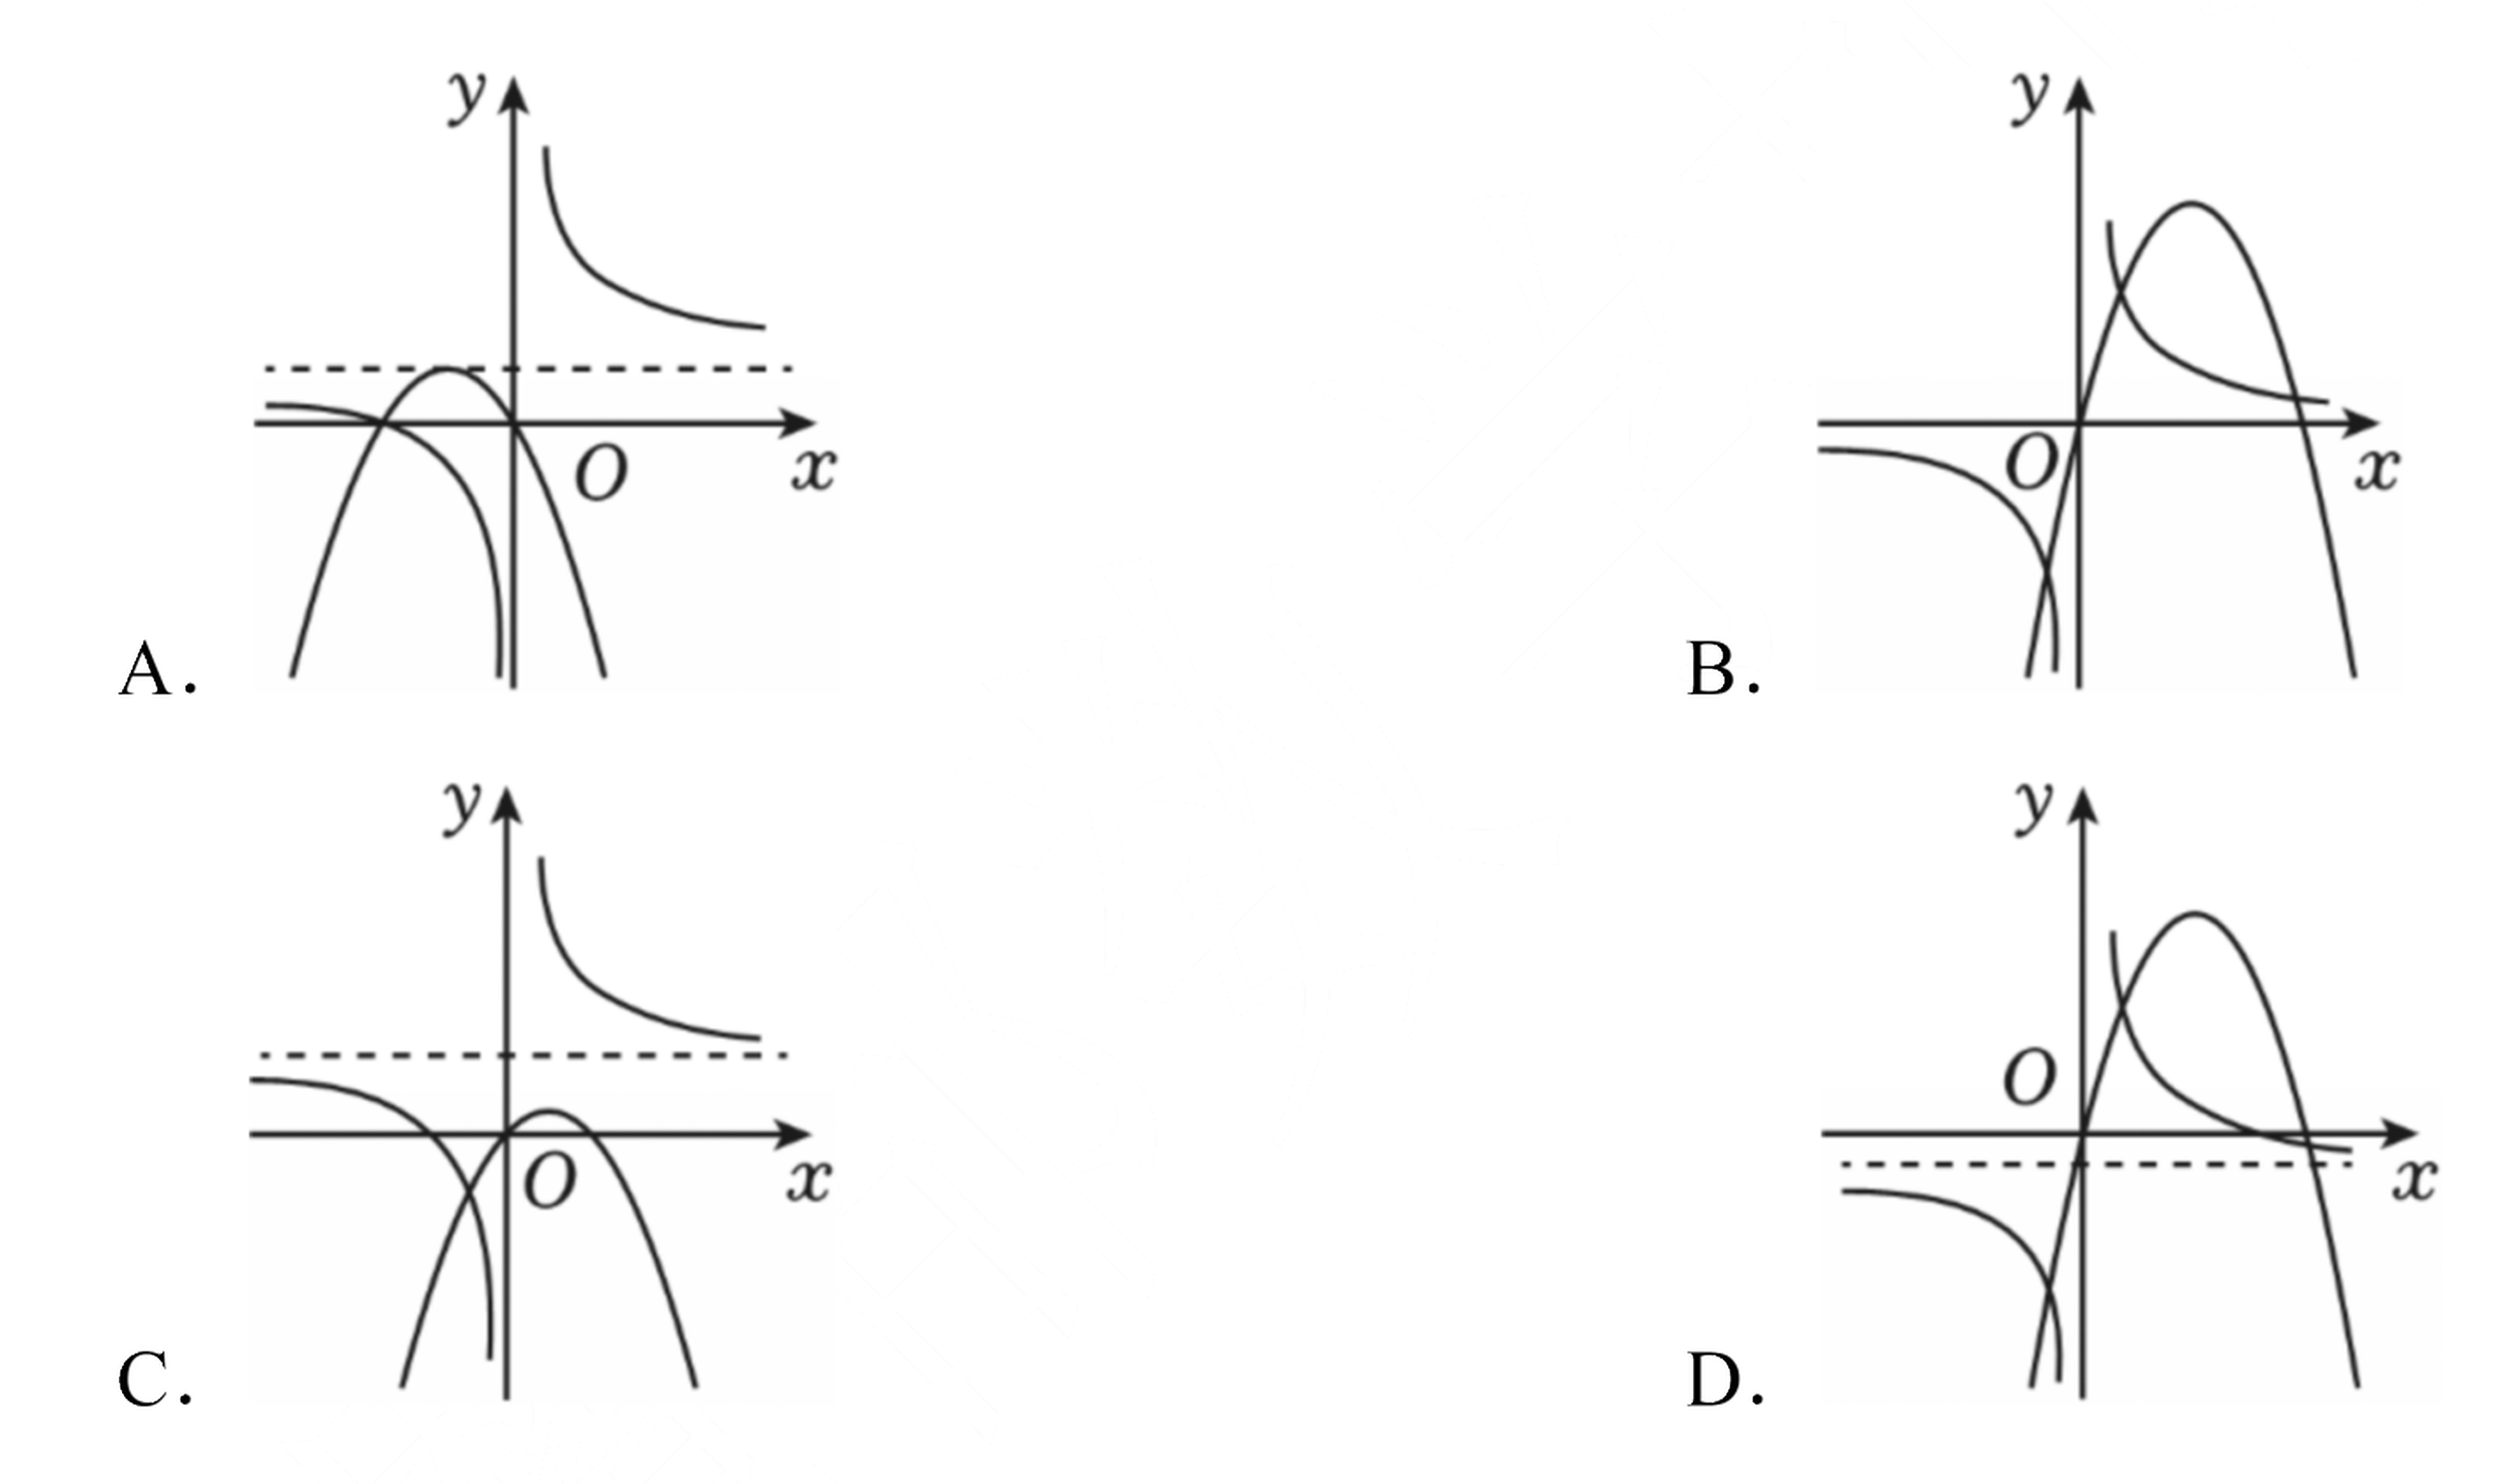
\includegraphics[width=0.80\textwidth]{figures/gao161_q14.png}
\end{center}

\ifanswer
\solbegin
\step{$A$ 选项，由二次函数图象得 $a<0$，$b<0$，由幂函数型函数图象得 $a<0$，$b>0$，}
\step{故 $A$ 选项错误；}
\step{$B$ 选项，由二次函数图象得 $a<0$，$b>0$，由幂函数型函数图象得 $a<0$，$b=0$，}
\step{故 $B$ 选项错误；}
\step{$C$ 选项，由二次函数图象得 $a<0$，$b>0$，由幂函数型函数图象得 $a<0$，$b>0$，}
\step{故 $C$ 选项正确；}
\step{$D$ 选项，由二次函数图象得 $a<0$，$b>0$，由幂函数型函数图象得 $a<0$，$b<0$，}
\step{故 $D$ 选项错误.}
\step{故选 $C$.}
\solend
\fi

% === Q15 === \subseteq／\subset、\varnothing、\mid；"排除 C""排除 B、D"正体字母照录；解析 4 行，故选 $A$
\item 设不等式 $\lvert f(x)\rvert+\lvert g(x)\rvert<a$（常数 $a>0$）的解集是 $M$，设不等式 $\lvert f(x)+g(x)\rvert<a$（常数 $a>0$）的解集是 $N$，则\mbox{（\quad）}

\keepwithprev
A. $M\subseteq N$\qquad B. $N\subseteq M$\qquad C. $M\subset N$\qquad D. $N\subset M$

\ifanswer
\solbegin
\step{$x\in M\Rightarrow\lvert f(x)+g(x)\rvert\leqslant\lvert f(x)\rvert+\lvert g(x)\rvert<a\Rightarrow x\in N$，所以 $M\subseteq N$.}
\step{取 $f(x)=g(x)=0$，则 $M=N$，排除 C.}
\step{取 $f(x)=1$，$g(x)=-1$，$a=1$，则 $M=\varnothing$，$N$ 为全体实数，排除 B、D.}
\step{故选 $A$.}
\solend
\fi

% === Q16 === "人文集"定义证明；cases 无；解析 21 行，故选 $B$
\item 设集合 $I_n=\{1,2,\cdots,n\}$，$n\in\N,n\geqslant1$，集合 $P_n=\left\{\dfrac{m}{\sqrt k}\mid m\in I_n,k\in I_n\right\}$，若 $P_n$ 的子集 $A$ 中任意两个元素之和不是整数的平方，则称 $A$ 为 “人文集”. 那么使 $P_n$ 能分成两个交集为空集的 “人文集” 的并集，且这两个人文集的并集恰为 $P_n$ 时，$n$ 的最大值是\mbox{（\quad）}

\keepwithprev
A. 13\qquad B. 14\qquad C. 15\qquad D. 16

\ifanswer
\solbegin
\step{先证当 $n\geqslant15$ 时，$P_n$ 不能分成两个不相交的人文集的并集.}
\step{假设当 $n\geqslant15$ 时，$P_n$ 可以分成两个不相交的人文集的并集，}
\step{设 $A$ 和 $B$ 为两个不相交的人文集，使 $A\cup B=P_n\supseteq I_n$.}
\step{不妨设 $1\in A$，则由于 $1+3=2^2$，所以 $3\notin A$，即 $3\in B$.}
\step{同理可得，$6\in A$，$10\in B$. 又推出 $15\in A$，}
\step{但 $1+15=4^2$，这与 $A$ 为人文集相矛盾.}
\step{再证 $P_{14}$ 满足要求. 当 $k=1$ 时，$P_{14}=\left\{\dfrac{m}{\sqrt k}\mid m\in I_{14},k\in I_{14}\right\}$，}
\step{可以分成 2 个人文集的并集.}
\step{事实上，只要取 $A_1=\{1,2,4,6,9,11,13\}$，$B_1=\{3,5,7,8,10,12,14\}$，}
\step{则 $A_1$ 和 $B_1$ 都是人文集，且 $A_1\cup B_1=P_{14}$.}
\step{当 $k=4$ 时，集合 $\left\{\dfrac{m}{\sqrt k}\mid m\in I_{14}\right\}$ 中，除整数外，}
\step{剩下的数组成集合 $\left\{\dfrac12,\dfrac32,\dfrac52,\cdots,\dfrac{13}{2}\right\}$，}
\step{可以分为下列 2 个人文集的并：$A_2=\left\{\dfrac12,\dfrac52,\dfrac92,\dfrac{11}{2}\right\}$，$B_2=\left\{\dfrac32,\dfrac72,\dfrac{13}{2}\right\}$.}
\step{当 $k=9$ 时，集合 $\left\{\dfrac{m}{\sqrt k}\mid m\in I_{14}\right\}$ 中，除整数外，}
\step{剩下的数组成集合 $\left\{\dfrac13,\dfrac23,\dfrac43,\dfrac53,\cdots,\dfrac{13}{3},\dfrac{14}{3}\right\}$，}
\step{可以分为下列 2 个人文集的并：$A_3=\left\{\dfrac13,\dfrac43,\dfrac53,\dfrac{10}{3},\dfrac{13}{3}\right\}$，$B_3=\left\{\dfrac23,\dfrac73,\dfrac83,\dfrac{11}{3},\dfrac{14}{3}\right\}$.}
\step{最后，集合 $C=\left\{\dfrac{m}{\sqrt k}\mid m\in I_{14},k\in I_{14},k\ne1,4,9\right\}$ 中的数的分母都是无理数，}
\step{它与 $P_n$ 中的任何其他数之和都不是整数，}
\step{因此，令 $A=A_1\cup A_2\cup A_3\cup C$，$B=B_1\cup B_2\cup B_3$，}
\step{则 $A$ 和 $B$ 是不相交的人文集，且 $A\cup B=P_{14}$.}
\step{综上，$n$ 的最大值为 14，故选 $B$.}
\solend
\fi

\end{enumerate}

\bigsec{三、解答题}

\begin{enumerate}
\setcounter{enumi}{16}

% === Q17 === "图像"照录；\Z；cases 块；解析 9 行，跨 06—07 页
\item (1) 已知函数 $y=x^{\frac{4m-m^2}{2}}$（$m\in\Z$）在区间 $(0,+\infty)$ 上是严格增函数，它的图像关于 $y$ 轴对称，求 $m$ 的值及该函数的解析式；

(2) 若 $(a-2)^{\frac32}<(1+2a)^{\frac32}$，求实数 $a$ 的取值范围.

\ifanswer
\solbegin
\step{(1) 由幂函数在 $(0,+\infty)$ 上严格递增，得 $\dfrac{4m-m^2}{2}>0\Leftrightarrow0<m<4$，}
\step{又 $m\in\Z$，所以 $m\in\{1,2,3\}$.}
\step{当 $m=1$ 或 $m=3$ 时，函数为 $y=x^{\frac32}$，定义域为 $[0,+\infty)$，}
\step{图像不关于 $y$ 轴对称.}
\step{当 $m=2$ 时，函数为 $y=x^2$，满足题意，所以 $m=2$，解析式 $y=x^2$.}
\step{(2) 原不等式有意义，须满足 $\begin{cases}a-2\geqslant0\\1+2a\geqslant0\end{cases}\Leftrightarrow a\geqslant2$，}
\step{函数 $y=x^{\frac32}$ 在 $[0,+\infty)$ 上严格递增，}
\step{因此 $(a-2)^{\frac32}<(1+2a)^{\frac32}\Leftrightarrow a-2<1+2a\Leftrightarrow a>-3$，}
\step{结合 $a\geqslant2$，得 $a\in[2,+\infty)$.}
\solend
\fi

% === Q18 === 题干"$a\geqslant0$"与解析"$a<0$"自相矛盾照录；"$A\cap B=(-2,-1]\cap[2,6)$"误印 ∩ 照录；\subseteq；解析 10 行
\item 已知实数 $a\geqslant0$，集合 $A=\left\{x\mid\dfrac{x+2}{x-6}<0\right\}$，$B=\{x\mid\lvert2x-1\rvert\geqslant3\}$，$C=\{x\mid x^2-3ax+2a^2<0\}$，

(1) 求 $A\cap B$；

(2) 若 $C\subseteq(A\cap B)$，求 $a$ 的取值范围.

\ifanswer
\solbegin
\step{(1) 由 $\dfrac{x+2}{x-6}<0$ 得 $-2<x<6$，即 $A=\{x\mid-2<x<6\}=(-2,6)$，}
\step{由 $\lvert2x-1\rvert\geqslant3$ 得 $2x-1\geqslant3$ 或 $2x-1\leqslant-3$，解得 $x\geqslant2$ 或 $x\leqslant-1$，}
\step{即 $B=(-\infty,-1]\cup[2,+\infty)$，}
\step{所以 $A\cap B=(-2,-1]\cap[2,6)$；}% 原卷把 ∪ 误印成 ∩，照录未改（见 ⑤ 2）
\step{(2) 由 (1) 得 $A\cap B=\{x\mid-2<x\leqslant-1\text{ 或 }2\leqslant x<6\}$，}
\step{因为 $C\subseteq(A\cap B)$，$x^2-3ax+2a^2=(x-a)(x-2a)<0$，}% 题干 $a\geqslant0$ 与解析 $a<0$ 自相矛盾，照录未改（见 ⑤ 1）
\step{当 $a=0$ 时，$C=\varnothing$，符合题意；}
\step{当 $a>0$ 时，$C=(a,2a)$，则 $\begin{cases}a\geqslant2\\2a\leqslant6\\a>0\end{cases}$，解得 $2\leqslant a\leqslant3$，}
\step{当 $a<0$ 时，$C=(2a,a)$，则 $\begin{cases}2a\geqslant-2\\a\leqslant-1\\a<0\end{cases}$，解得 $a=-1$，}
\step{故 $a$ 的范围为 $\{-1,0\}\cup[2,3]$.}
\solend
\fi

% === Q19 === 双碳太阳能应用题；"双碳""自发自用、市电互补"弯引号；解析 8 行，跨 08 页上下
\item 为响应 “双碳” 目标，某电子企业拟安装一套可使用 10 年的太阳能供电设备. 该设备的安装费用 $P(x)$（单位：万元）与太阳能电池板面积 $x(x>0)$（单位：平方米）成正比，比例系数为 $\dfrac12$. 为保障生产用电，安装后采用 “自发自用、市电互补” 模式，在此模式下，企业每年消耗的电费 $Q(x)$（单位：万元）与安装的这种太阳能电池板的面积 $x$ 之间的函数关系是 $Q(x)=\dfrac{180}{x+5}$. 记 $W(x)$（单位：万元）为该企业安装这种太阳能供电设备的费用与 10 年所消耗的电费之和.

(1) 要使该设备的安装费与第 1 年的电费之和不超过 17 万元，求安装太阳能电池板面积 $x$ 的取值范围；

(2) 当 $x$ 为多少平方米时，$W(x)$ 取得最小值？最小值是多少万元？

\ifanswer
\solbegin
\step{(1) $P(x)=\dfrac{x}{2}$，安装费与第 1 年的电费之和不超过 17 万元，即 $\dfrac{x}{2}+\dfrac{180}{x+5}\leqslant17$，}
\step{$x>0$，上式等价于 $x^2-29x+190\leqslant0\Leftrightarrow(x-10)(x-19)\leqslant0$，}
\step{解得 $x\in[10,19]$.}
\step{(2) 安装费用与 10 年电费之和为 $W(x)=P(x)+10Q(x)$，}
\step{$=\dfrac{x}{2}+\dfrac{1800}{x+5}=\dfrac{x+5}{2}+\dfrac{1800}{x+5}-\dfrac52$，}
\step{$x>0$，由基本不等式得 $W(x)\geqslant2\sqrt{\dfrac{x+5}{2}\cdot\dfrac{1800}{x+5}}-\dfrac52=60-\dfrac52=57.5$，}
\step{等号当且仅当 $\dfrac{x+5}{2}=\dfrac{1800}{x+5}$，即 $x=55$ 时成立.}
\step{因此，当电池板面积为 55 平方米时，$W(x)$ 取得最小值 57.5 万元.}
\solend
\fi

% === Q20 === $a*b$ 定义；\min 改正体；cases 块；解析 23 行，跨 08—10 页
\item 设 $a$、$b\in\R$，定义 $a*b=\begin{cases}a,&a<b\\b,&a\geqslant b\end{cases}$.

(1) 若 $x*2>1$，求 $x$ 的取值范围；

(2) 若 $(\lvert x-1\rvert+\lvert x-2\rvert)*3=3$，求 $x$ 的取值范围；

(3) 若 $a$、$b>0$，记 $M=a*\dfrac{b}{a^2+4b^2}$，分别比较 $M$ 与 $a$，以及 $M$ 与 $\dfrac{b}{a^2+4b^2}$ 的大小，并求 $M$ 的最大值.

\ifanswer
\solbegin
\step{(1) 定义 $a*b=\begin{cases}a,&a<b\\b,&a\geqslant b\end{cases}$，由 $x*2>1$，得 $\begin{cases}x<2\\x>1\end{cases}$，或 $\begin{cases}x\geqslant2\\2>1\end{cases}$，}
\step{解得 $x>1$，即 $x$ 的取值范围为 $\{x\mid x>1\}$；}
\step{(2) 当 $x\geqslant2$ 时，$\lvert x-1\rvert+\lvert x-2\rvert=2x-3\geqslant1$，}
\step{当 $1\leqslant2x-3\leqslant3$，即 $2\leqslant x\leqslant3$ 时，}
\step{此时 $(\lvert x-1\rvert+\lvert x-2\rvert)*3=2x-3=3$，解得 $x=3$；}
\step{当 $2x-3>3$，即 $x>3$ 时，}
\step{此时 $(\lvert x-1\rvert+\lvert x-2\rvert)*3=3$ 恒成立，则 $x>3$；}
\step{当 $-2x+3>3$，即 $x<0$ 时，}
\step{此时 $(\lvert x-1\rvert+\lvert x-2\rvert)*3=3$ 恒成立，则 $x<0$.}
\step{当 $1<x<2$ 时，$\lvert x-1\rvert+\lvert x-2\rvert=1$，}
\step{此时 $(\lvert x-1\rvert+\lvert x-2\rvert)*3=1\ne3$，不符合题意；}
\step{当 $x\leqslant1$ 时，$\lvert x-1\rvert+\lvert x-2\rvert=-2x+3\geqslant1$，}
\step{当 $-2x+3\leqslant3$，即 $0\leqslant x\leqslant1$ 时，}
\step{此时 $(\lvert x-1\rvert+\lvert x-2\rvert)*3=-2x+3=3$，解得 $x=0$.}
\step{综上所述，$x$ 的取值范围为 $\{x\mid x\leqslant0\text{ 或 }x\geqslant3\}$；}
\step{(3) 由题意，$M=a*\dfrac{b}{a^2+4b^2}=\min\left\{a,\dfrac{b}{a^2+4b^2}\right\}$，}% 原卷印斜体 min，按全稿惯例改正体 \min（见 ② ⑬）
\step{则 $M\leqslant a$，$M\leqslant\dfrac{b}{a^2+4b^2}$.}
\step{因为 $a$、$b>0$，所以 $\dfrac{b}{a^2+4b^2}\leqslant\dfrac{b}{2\sqrt{a^2\cdot4b^2}}=\dfrac{1}{4a}$，}
\step{当且仅当 $a=2b>0$ 时取等号，}
\step{当 $a\geqslant\dfrac{1}{4a}$，即 $a\geqslant\dfrac12$ 时，$M=a*\dfrac{b}{a^2+4b^2}=\dfrac{b}{a^2+4b^2}\leqslant\dfrac{1}{4a}$，}
\step{则 $a=\dfrac12$，$b=\dfrac14$ 时，$M$ 取得最大值 $\dfrac12$；}
\step{当 $0<a<\dfrac12$ 时，$M=a*\dfrac{b}{a^2+4b^2}=a$，此时 $M<\dfrac12$.}
\step{综上所述，$M$ 的最大值为 $\dfrac12$.}
\solend
\fi

% === Q21 === $A_n$／$B_n$／$S_n$／$T_n$ 新定义；题干第 3 问误标 (2) 照录、解析作 (3)；\prec；解析 25 行，跨 10—11 页
\item 对任意正整数 $n$，记集合 $A_n=\{(a_1,a_2,\cdots,a_n)\mid a_1,a_2,\cdots,a_n$ 均为非负整数，且 $a_1+a_2+\cdots+a_n=n\}$，集合 $B_n=\{(b_1,b_2,\cdots,b_n)\mid b_1,b_2,\cdots,b_n$ 均为非负整数，且 $b_1+b_2+\cdots+b_n=2n\}$. 设 $\alpha=(a_1,a_2,\cdots,a_n)\in A_n$，$\beta=(b_1,b_2,\cdots,b_n)\in B_n$，若对任意 $i\in\{1,2,\cdots,n\}$ 都有 $a_i\leqslant b_i$，则记 $\alpha\prec\beta$.

(1) 写出集合 $A_2$ 和 $B_2$；

(2) 证明：对任意 $\alpha\in A_n$，存在 $\beta\in B_n$，使得 $\alpha\prec\beta$；

(2) 设集合 $S_n=\{(\alpha,\beta)\mid\alpha\in A_n,\beta\in B_n,\alpha\prec\beta\}$，求证：$S_n$ 中的元素个数是完全平方数.% 原卷第 3 问题干误标 (2)（与第 2 问重号），照录未改（见 ⑤ 3）

\ifanswer
\solbegin
\step{(1) $A_2=\{(0,2),(1,1),(2,0)\}$，$B_2=\{(0,4),(1,3),(2,2),(3,1),(4,0)\}$；}
\step{(2) 对任意 $\alpha=(a_1,a_2,\cdots,a_n)\in A_n$，设 $b_i=a_i+1$（$i=1,2,3,\cdots,n$），}
\step{则 $b_1,b_2,\cdots,b_n$ 均为非负整数，且 $a_i\leqslant b_i$（$i=1,2,3,\cdots,n$）.}
\step{令 $\beta=(b_1,b_2,\cdots,b_n)$，则 $b_1+b_2+\cdots+b_n$}
\step{$=(a_1+1)+(a_2+1)+\cdots+(a_n+1)=(a_1+a_2+\cdots+a_n)+n=2n$，}
\step{所以 $\beta\in B_n$，且 $\alpha\prec\beta$.}
\step{(3) 对任意 $\alpha=(a_1,a_2,\cdots,a_n)\in A_n$，$\alpha'=(a_1',a_2',\cdots,a_n')\in A_n$，}
\step{记 $\alpha+\alpha'=(a_1+a_1',a_2+a_2',\cdots,a_n+a_n')$，}
\step{则 $a_1+a_1',a_2+a_2',\cdots,a_n+a_n'$ 均为非负整数，}
\step{且 $(a_1+a_1')+(a_2+a_2')+\cdots+(a_n+a_n')$}
\step{$=(a_1+a_2+\cdots+a_n)+(a_1'+a_2'+\cdots+a_n')=n+n=2n$，}
\step{所以 $\alpha+\alpha'\in B_n$，且 $\alpha\prec\alpha+\alpha'$，$\alpha'\prec\alpha+\alpha'$.}
\step{设集合 $A_n$ 中的元素个数为 $t$，设 $A_n=\{\alpha_1,\alpha_2,\cdots,\alpha_t\}$.}
\step{设集合 $T_n=\{(\alpha_i,\alpha_i+\alpha_j)\mid i=1,2,\cdots,t,j=1,2,\cdots,t\}$.}
\step{对任意 $\alpha_i\in A_n$（$i=1,2,\cdots,t$），都有 $\alpha_i+\alpha_1,\alpha_i+\alpha_2,\cdots,\alpha_i+\alpha_t\in B_n$，}
\step{且 $\alpha_i\prec\alpha_i+\alpha_j$，$j=1,2,\cdots,t$，所以 $T_n\subseteq S_n$.}
\step{若 $(\alpha,\beta)\in S_n$，其中 $\alpha=(a_1,a_2,\cdots,a_n)\in A_n$，$\beta=(b_1,b_2,\cdots,b_n)\in B_n$，}
\step{设 $c_i=b_i-a_i$（$i=1,2,\cdots,n$），因为 $a_i\leqslant b_i$，所以 $c_i=b_i-a_i\geqslant0$，}
\step{记 $\alpha'=(c_1,c_2,\cdots,c_n)$，}
\step{则 $c_1+c_2+\cdots+c_n=(b_1-a_1)+(b_2-a_2)+\cdots+(b_n-a_n)$}
\step{$=(b_1+b_2+\cdots+b_n)-(a_1+a_2+\cdots+a_n)=2n-n=n$，}
\step{所以 $\alpha'\in A_n$，并且有 $\beta=\alpha+\alpha'$，所以 $(\alpha,\beta)\in T_n$，所以 $S_n\subseteq T_n$，}
\step{所以 $S_n=T_n$.}
\step{因为集合 $T_n$ 中的元素个数为 $t^2$，所以 $S_n$ 中的元素个数为 $t^2$，}
\step{是完全平方数.}
\solend
\fi

\end{enumerate}

\end{document}
"
%
% ① 原始材料：微信公众号"魔都数学加油站"文章，连载"27学年高一161"，原卷卷面标题
% "2026-2027 年松江一中嘉一实验高一上期中"（卷面未印副标题、未印连载号）。
% 正文为 11 张 PNG 页（01/02/03/05/06/07/08/09/11 为 4762×6735，04/10 为
% 2560×3620，同一篇各页分辨率混排，逐页按各自分辨率裁图核对）。
% 体例：讲评版——填空 3—12（10 题）、选择 13—16（4 题）、解答 17—21（5 题），
% 共 19 题，自第 3 题起编（1、2 未印在本篇）；Q13 答案"A"直接印在题干括号内、
% 且无【答案】/【解析】段，本稿按 高一37 第 13 题／高一57 第 13 题成例把括号
% 留空、另提 \ans{$A$}；其余 18 题逐题印【解析】、用 \solbegin…\solend。
% 题目、答案、解析均据原图转录；卷面粉红色水印"魔都数学加油站"及公众号页脚未录入。
% 全卷插图清单（逐页通读 11 页确认）：仅 1 组——Q14 四幅图像选项（04 页 2×2
% 排布，二次函数与幂函数型函数在同一坐标系中的图象，A/B/C/D 四幅小图），
% 合并成一张，三版都出，裁 figures/gao161_q14.png。其余各页逐页确认无其它
% 题目配图、无解析内配图、无表格、无"如图"处（Q16 解析里的"可以分为下列 2 个
% 人文集的并"是纯文字＋集合，不是表格；OCR 里看似表格的行实为大括号与分数）。
%
% 卷首标题：原卷印作"2026-2027 年松江一中嘉一实验高一上期中"，年份区间按全稿惯例排 en dash；
% 原卷卷面未印副标题，本稿按同期中卷知识模块口径补出"集合与常用逻辑用语、不等式、函数"。
%
% ② 与原卷的排版差异／照录项清单：
%   ① 原文从第 3 题起，本稿保留原题号；共 19 题三节，解答题 5 题到 21；
%      三节各自一个 enumerate + \setcounter{enumi}{2}/{12}/{16}（不贯穿），
%      用 \examtitlest[3] 起手；
%   ② 混合体例：Q13 原卷把答案"A"直接印在题干括号内（"（  A  ）"）、且题下
%      无【答案】/【解析】段，按 高一37 第 13 题／高一57 第 13 题成例把括号
%      留空、另提 \ans{$A$}、不补造解析；其余 18 题印【解析】、用
%      \solbegin…\solend；四道选择题中 Q14/Q15/Q16 的答案在解析末句
%      "故选 $C$／$A$／$B$"、Q13 用 \ans{$A$}；括号 \mbox{（\quad）} 留空；
%      答案版【答案】/【解析】标记数 = 19 = 全卷题数（1 个 \ans ＋ 18 个 \solbegin）；
%   ③ 原卷卷面未印副标题，本稿按知识模块口径补出；
%   ④ 原卷填空横线按全稿惯例排 \blankline[4.4em]；选择题选项段前按惯例各加
%      \keepwithprev；Q14 四幅选项图整块用 \needvspace{9cm} 守卫（守卫放
%      \item 之前，见 高一132 Q14／高一154 Q15 成例）；解答题不留作答区、
%      不加 \anspace（原卷为讲评版）；
%   ⑤ 数集归一：Q8"$x\in\R$"、Q11"$m\in\R$"、Q13"$x,y\in\N$"、
%      Q16"$n\in N$"、Q17"$m\in\Z$"、Q20"$a$、$b\in R$"——原卷印正体粗体
%      或斜体 R/N/Z，按全稿惯例归一 \R／\N／\Z；绝对值排 \lvert…\rvert
%      （Q9、Q12、Q15、Q18、Q20），集合描述竖线排 \mid（Q12、Q16、Q18、
%      Q20、Q21），空集 \varnothing（Q15、Q18），补集无用例，不等号按全稿
%      惯例排 \leqslant／\geqslant；
%   ⑥ 子集符号逐处照录不统一：Q12 cases 定义"$C(A)\geqslant C(B)$"、
%      Q15 选项 A/B"$M\subseteq N$""$N\subseteq M$"与解析"$M\subseteq N$"
%      印带下划线 ⊆（照录 \subseteq），Q15 选项 C/D"$M\subset N$""$N\subset M$"
%      印单线 ⊂（照录 \subset），Q18 "$C\subseteq(A\cap B)$"、Q21
%      "$T_n\subseteq S_n$""$S_n\subseteq T_n$"均带下划线照录 \subseteq；
%      本卷无 \not\subset 用例；
%   ⑦ 判别式：Q7 解析"$\Delta=(m-6)(m+2)>0$"、Q8 解析"$\Delta=a^2-4a<0$"、
%      Q12 解析"$\Delta=a^2-8$"共 3 处，逐处放大确认印等腰偏高粗三角
%      （高>宽、右斜边粗），照录 \Delta；本卷无扁等边细线 \triangle 用例；
%   ⑧ 中文弯引号照录：Q7"$m\geqslant6$""有两个不相等的正实数根"及四个
%      条件短语、Q13 反证法命题、Q16"人文集"、Q19"双碳""自发自用、市电互补"；
%      注释里一律 ASCII 引号；数学式内 CJK 用 \text{}（Q18、Q20 解集描述内"或"）；
%   ⑨ "图像／图象"逐处照录不统一：Q4"的图像"、Q17 题干"它的图像关于 $y$ 轴
%      对称"及解析"图像不关于 $y$ 轴对称"印"图像"；Q14 题干"的图象可能为"
%      与解析 A/B/C/D 四行各"由二次函数图象得""由幂函数型函数图象得"
%      共 8 处印"图象"（象，无亻）；
%   ⑩ 文本圈数字逐处照录：Q12 题干①②③④、Q12 解析"故①错误""故②正确"
%      "故③正确""故④错误""故正确的是②③"，均为印刷圈数字（文本模式）；
%   ⑪ 半角逗号在数学组之间是全稿惯例、非笔误，逐处照录（Q5"$a$、$b$"、
%      Q13"$x,y\in\N$"、Q16"$n\in\N,n\geqslant1$"与集合描述内逗号、
%      Q20"$a,b\in\R$"、Q21 各集合描述内逗号）；行末西文句点 ASCII `.`；
%      原卷行中句点（Q16"$10\in B$. 又推出 $15\in A$"、Q16"再证 $P_{14}$
%      满足要求. 当 $k=1$ 时"、Q18"$A\cap B=(-2,-1]\cap[2,6)$；"后的分号）
%      按全稿惯例一律排 ASCII `.`／全角"；"；中文语境行中全角逗号／顿号照录；
%   ⑫ 原卷数学式内联条件（Q14"$y=x^a+b(a\ne0)$"、Q19"$x(x>0)$"、
%      Q11"$\lvert x-m\rvert<n\,(m\in\R,n>0)$"）印半角括号，逐处照录未改
%      全角（同 高一147 口径）；
%      中文语境的括注（Q5"结果用 $a$、$b$ 表示"、Q7"填…"、Q12"填写序号"、
%      Q15"常数 $a>0$"、Q19"单位：万元"）印全角括号，照录；
%   ⑬ 复杂式照录别简化：Q3 $(a^{2-\sqrt3})^{2+\sqrt3}\times\sqrt{a^2}\times
%      b^{\sqrt3}\times b^{1-\sqrt3}$ 与 $a^{(2-\sqrt3)(2+\sqrt3)}\cdot a\cdot
%      b^{\sqrt3+1-\sqrt3}=a\cdot a\cdot b=a^2b$（题干用 \times、解析用 \cdot，
%      逐处照录不统一，见 ⑤）；Q5 $\dfrac{\lg2}{\lg2+\lg3}=\dfrac{a}{a+b}$、
%      Q10 $t-\dfrac3t=2$ 与 $b=a^3$、$ab=a^4=2$、Q11 $\left(2a-\dfrac12
%      -a+\dfrac12,2a-\dfrac12+a-\dfrac12\right)=(a,3a-1)$ 与
%      $\left(\dfrac43,\dfrac53\right]\cup\{2\}$、Q16 各分数集合、Q19
%      $x^2-29x+190\leqslant0$ 与 $W(x)=P(x)+10Q(x)$ 与
%      $2\sqrt{\dfrac{x+5}{2}\cdot\dfrac{1800}{x+5}}-\dfrac52=60-\dfrac52=57.5$、
%      Q20 $M=a*\dfrac{b}{a^2+4b^2}=\min\left\{a,\dfrac{b}{a^2+4b^2}\right\}$
%      与 $\dfrac{b}{2\sqrt{a^2\cdot4b^2}}=\dfrac{1}{4a}$、Q21 各 $A_n$／$B_n$／
%      $T_n$ 定义；\left…\right 不得拆到不同 $…$ 组（Q11 的 \left(…\right)、
%      Q11 的 \left(\dfrac43,\dfrac53\right]、Q16 的 \left\{\dfrac{m}{\sqrt k}
%      \mid…\right\} 与 \left\{\dfrac12,\dfrac32,\dfrac52,\cdots,\dfrac{13}{2}\right\}
%      等、Q20 的 \min\left\{…\right\}）；cases 块整体算一个印刷行
%      （Q12 定义、Q17 (2)、Q18 (2) 两处、Q20 定义与 (1)）；原卷 Q20 解析
%      "$=min\{…\}$"印斜体 min，按 高一122／高一102 成例改正体 \min；
%   ⑭ 一条 \step = 原卷解析的一个印刷行；别并折行、别拆行。跨页续印按题合并
%      （Q6 的 01 页上下题干重复印、Q10 的 01—02 页、Q11 的 02—03 页、
%      Q12 的 03—04 页、Q16 的 05—06 页、Q17 的 06—07 页、Q18 的 07 页
%      上下、Q19 的 08 页上下、Q20 的 08—10 页、Q21 的 10—11 页）；
%      跨半页重叠行（Q10"令 $t=\log_a b>0$…"、Q16"它与 $P_n$ 中的任何
%      其他数之和都不是整数，"、Q18"【解析】(1) 由 $\dfrac{x+2}{x-6}<0$…"、
%      Q19"$x>0$，上式等价于…"、Q20"此时…则 $x<0$."、Q21"若 $(\alpha,\beta)
%      \in S_n$…"与"设 $c_i=b_i-a_i$…"）只算一个印刷行；
%   ⑮ 自定义记号照录：Q12"$C(A)$""$A*B$""$S$"、Q16"$I_n$""$P_n$""人文集"
%      "$A_1$／$B_1$／$A_2$／$B_2$／$A_3$／$B_3$／$C$"、Q20"$a*b$""$M$"、
%      Q21"$A_n$／$B_n$／$S_n$／$T_n$""$\alpha\prec\beta$""$\alpha+\alpha'$"；
%   ⑯ 选项字母体例照录不统一：Q15 解析"排除 C.""排除 B、D."两处原卷印
%      正体（文本模式），Q13 \ans{$A$}、Q14"$A$ 选项"…"故选 $C$"、
%      Q15"故选 $A$"、Q16"故选 $B$"用斜体（数学模式），逐处照录、不统一；
%   ⑰ 红字：全卷逐页扫描无红色加粗小标题（仅粉色水印），故本卷无 \stepm，
%      不引入红色定义；
%
% ③ 行数复核：一条 \step = 原卷解析的一个印刷行，cases 块作一个印刷行计。
%   逐题数（逐页核对定稿）：Q3：1；Q4：1；Q5：1；Q6：3；Q7：4；Q8：4；
%   Q9：2；Q10：2；Q11：7；Q12：8；Q13：0（答案印括号内、提 \ans{}，
%   不计入 \step 账）；Q14：9；Q15：4；Q16：21；Q17：9；Q18：10；Q19：8；
%   Q20：23；Q21：25。
%   合计 142 行（142 条 \step，无 \stepm），与原卷逐题印刷行相等。
%   全卷 19 题：Q13 一处 \ans{} ＋ 其余 18 题设 \solbegin…\solend，
%   答案版【答案】/【解析】标记数 = 19 = 全卷题数。
%
% ④ 页码分布（供回原图复核）：
%   卷首标题＋"一、填空题"＋Q3/Q4/Q5 题干＋解析各 1 行＋Q6 题干首行
%   在 01 页上半；Q6 题干（重复印）＋解析 3 行＋Q7 题干＋解析 4 行在
%   01 页下半；Q8 题干＋解析 4 行＋Q9 题干＋解析 2 行＋Q10 题干＋
%   解析首行在 02 页上半；Q10 解析（重复印）＋末行＋Q11 题干＋解析
%   前 3 行在 02 页下半；Q11 解析后 4 行＋Q12 题干＋cases 定义＋①
%   在 03 页上半；Q12 ②③④ 三命题＋"填写序号"行＋解析前 6 行在
%   03 页下半；Q12 解析后 2 行＋"二、选择题"标题＋Q13 题干＋选项＋
%   Q14 题干＋"（　）"＋A/B 两幅图在 04 页上半；Q14 四幅图（重复印）
%   ＋解析 9 行在 04 页下半；Q15 题干＋选项＋解析 4 行＋Q16 题干＋
%   选项在 05 页上半；Q16 题干（重复印）＋选项＋解析前 10 行在 05 页
%   下半；Q16 解析中 8 行（k=4、k=9 两批＋集合 C＋"它与 $P_n$…"）
%   在 06 页上半；Q16 解析"它与 $P_n$…"（重复印）＋末 3 行＋
%   "三、解答题"标题＋Q17 题干＋两问＋解析前 4 行在 06 页下半；
%   Q17 解析后 5 行＋Q18 题干＋两问＋解析首行在 07 页上半；Q18 解析
%   （重复首行）＋余 9 行在 07 页下半；Q19 题干＋两问＋解析前 2 行在
%   08 页上半；Q19 解析（重复第 2 行）＋余 6 行＋Q20 定义＋(1) 问在
%   08 页下半；Q20 (2)(3) 两问＋解析 (1) 2 行＋(2) 前 7 行在 09 页
%   上半；Q20 解析 (2) 余 4 行＋(3) 前 4 行在 09 页下半；Q20 解析 (3)
%   余 4 行＋Q21 题干＋三问在 10 页上半；Q21 题干（重复印）＋解析
%   (1)(2)(3) 前 8 行在 10 页下半；Q21 解析 (3) 中 10 行在 11 页上半；
%   Q21 解析 (3)（重复 2 行）＋末 7 行"是完全平方数."在 11 页下半。
%   本稿按题连排，不丢行、不并折行；全卷末题为第 21 题，无附加题节。
%
% ⑤ 存疑照录（放大原图确认，照录未改、正文对应处另有 % 注）：
%   1. Q18 题干印"已知实数 $a\geqslant0$"，解析却另设"当 $a<0$ 时"并解出
%      $a=-1$，末行答案"故 $a$ 的范围为 $\{-1,0\}\cup[2,3]$"含负数，
%      与题干 $a\geqslant0$ 自相矛盾——系原卷前后不一，照录未改（放大
%      07 页确认题干确印 $a\geqslant0$）；
%   2. Q18 解析"所以 $A\cap B=(-2,-1]\cap[2,6)$；"原卷把并集误印成
%      交集号 ∩（紧接下一行"$A\cap B=\{x\mid-2<x\leqslant-1$ 或
%      $2\leqslant x<6\}$"用"或"），照录未改（放大 07 页确认印 ∩）；
%   3. Q21 题干第 3 问原卷标号印作"(2)"（与第 2 问重号），而解析里
%      同一问标作"(3)"——原卷笔误，题干与解析逐处照录、不统一；
%   4. Q3 题干四处乘号印"×"（\times）、解析内三处乘号印"·"（\cdot），
%      逐处照录未统一（放大 01 页确认）；
%   5. Q16 解析"先证当 $n\geqslant15$ 时"印 ≥（非 >），与"综上，$n$
%      的最大值为 14"自洽，照录；题干"$n\in N,n\geqslant1$"印斜体
%      $N$、按全稿惯例归一 \N（见 ② ⑤）；
%   6. Q20 解析"$M=a*\dfrac{b}{a^2+4b^2}=min\{…\}$"原卷印斜体 min，
%      按全稿惯例改正体 \min（见 ② ⑬）；末行"$M$ 的最大值为
%      $\dfrac12$"照录；
%   7. Q15 解析"排除 C.""排除 B、D."用正体字母，而"故选 $A$"用斜体
%      字母，原卷体例不一（见 ② ⑯），照录未统一。
%   全卷除此 7 类外未发现其它笔误／自相矛盾处；Q13 只把答案印在括号内、
%   其余 18 题全部印【解析】。
%

\documentclass[a4paper,11pt]{article}
\usepackage{common}

\begin{document}

\examtitlest[3]{2026--2027 年松江一中嘉一实验高一上期中}{集合与常用逻辑用语、不等式、函数}

\bigsec{一、填空题}

\begin{enumerate}
\setcounter{enumi}{2}

% === Q3 === 题干 \times、解析 \cdot 逐处照录；解析 1 行
\item 设 $a>0$，$b>0$，化简 $(a^{2-\sqrt3})^{2+\sqrt3}\times\sqrt{a^2}\times b^{\sqrt3}\times b^{1-\sqrt3}=$\blankline[4.4em].

\ifanswer
\solbegin
\step{因为 $a>0$，所以 $\sqrt{a^2}=a$，原式 $=a^{(2-\sqrt3)(2+\sqrt3)}\cdot a\cdot b^{\sqrt3+1-\sqrt3}=a\cdot a\cdot b=a^2b$.}
\solend
\fi

% === Q4 === "图像"照录；解析 1 行
\item 若幂函数 $y=x^a$ 的图像经过点 $(5,\sqrt5)$，则此幂函数的表达式为 $y=$\blankline[4.4em].

\ifanswer
\solbegin
\step{$5^a=\sqrt5\Rightarrow a=\dfrac12$，所以 $y=\sqrt x$.}
\solend
\fi

% === Q5 === "结果用 $a$、$b$ 表示"全角括号＋顿号照录；解析 1 行
\item 已知 $\lg2=a$，$10^b=3$，则 $\log_6 2=$\blankline[4.4em]（结果用 $a$、$b$ 表示）.

\ifanswer
\solbegin
\step{$\lg3=b$，$\log_6 2=\dfrac{\lg2}{\lg2+\lg3}=\dfrac{a}{a+b}$.}
\solend
\fi

% === Q6 === 对称中心；解析 3 行，题干跨 01 页上下重复印
\item 若函数 $y=\dfrac{mx-1}{x+n}$ 的对称中心是 $(4,-3)$，则 $m+n=$\blankline[4.4em].

\ifanswer
\solbegin
\step{令 $x=-n+t$（$t\ne0$），则 $y-m=-\dfrac{mn+1}{t}$；}
\step{将 $t$ 换成 $-t$，$y-m$ 变为其相反数，因此对称中心为 $(-n,m)$.}
\step{于是 $n=-4$，$m=-3$，得 $m+n=-7$.}
\solend
\fi

% === Q7 === 充要条件；中文弯引号＋圈选条件；\Delta 高瘦；解析 4 行
\item 已知关于 $x$ 的一元二次方程 $x^2-mx+m+3=0$，则 “$m\geqslant6$” 是该方程 “有两个不相等的正实数根” 的\blankline[4.4em]条件（填 “充分不必要”、“必要不充分”、“充要” 或 “既不充分也不必要”）.

\ifanswer
\solbegin
\step{方程有两个不相等的正实数根}
\step{$\Leftrightarrow m>0$、$m+3>0$ 且 $\Delta=(m-6)(m+2)>0\Leftrightarrow m>6$.}
\step{$m>6\Rightarrow m\geqslant6$，但 $m=6$ 时方程有两个相等的正实数根，}
\step{因此为必要不充分条件.}
\solend
\fi

% === Q8 === \R、\Delta；解析 4 行
\item 对于任意的 $x\in\R$，代数式 $\lg(ax^2+ax+1)$ 都有意义，则实数 $a$ 的取值范围是\blankline[4.4em].

\ifanswer
\solbegin
\step{真数须满足 $ax^2+ax+1>0$ 对任意 $x\in\R$ 恒成立.}
\step{$a=0$ 时成立；}
\step{$a\ne0$ 时，恒成立等价于 $a>0$ 且 $\Delta=a^2-4a<0$，解得 $0<a<4$；}
\step{因此 $a\in[0,4)$.}
\solend
\fi

% === Q9 === 绝对值 \lvert…\rvert；解析 2 行
\item 若不等式 $\lvert x+1\rvert-\lvert x-4\rvert<m$ 的解集为非空集合，则实数 $m$ 的取值范围是\blankline[4.4em].

\ifanswer
\solbegin
\step{$\lvert x+1\rvert-\lvert x-4\rvert\geqslant-\lvert(x+1)-(x-4)\rvert=-5$，当 $x=-1$ 时取等号，}
\step{因此原不等式的解集非空 $\Leftrightarrow m>-5$，所求范围为 $(-5,+\infty)$.}
\solend
\fi

% === Q10 === 换底；$\log_2 a\cdot\log_2 b$；解析 2 行，跨 02 页上下
\item 已知 $a>1$，$b>1$，若 $\log_a b-3\log_b a=2$，且 $ab=2$，则 $\log_2 a\cdot\log_2 b=$\blankline[4.4em].

\ifanswer
\solbegin
\step{令 $t=\log_a b>0$，则 $t-\dfrac{3}{t}=2\Leftrightarrow(t-3)(t+1)=0$，得 $t=3$，}
\step{于是 $b=a^3$，$ab=a^4=2$，得 $\log_2 a=\dfrac14$，$\log_2 b=\dfrac34$，所求为 $\dfrac{3}{16}$.}
\solend
\fi

% === Q11 === 邻域定义；\left(…\right) 不拆组；解析 7 行，跨 02—03 页
\item 对于实数 $m$ 和正数 $n$，称满足不等式 $\lvert x-m\rvert<n\,(m\in\R,n>0)$ 的实数 $x$ 的集合叫做 $m$ 的 $n$ 邻域. 已知 $a>\dfrac12$，若 $2a-\dfrac12$ 的 $a-\dfrac12$ 邻域中恰有 2 个整数，则 $a$ 的取值范围是\blankline[4.4em].

\ifanswer
\solbegin
\step{所求邻域为 $\left(2a-\dfrac12-a+\dfrac12,2a-\dfrac12+a-\dfrac12\right)=(a,3a-1)$.}
\step{当 $\dfrac12<a\leqslant1$ 时至多含 1 个整数；}
\step{当 $a>2$ 时，区间长度 $2a-1>3$，至少含 3 个整数.}
\step{当 $1<a<2$ 时，区间必含 2，恰有两个整数等价于 $3<3a-1\leqslant4$，}
\step{即 $\dfrac43<a\leqslant\dfrac53$.}
\step{当 $a=2$ 时，区间为 $(2,5)$，恰含整数 $3,4$；}
\step{所以 $a\in\left(\dfrac43,\dfrac53\right]\cup\{2\}$.}
\solend
\fi

% === Q12 === $C(A)$／$A*B$ 定义题；①②③④ 文本圈数字；\subseteq／\subset、\Delta、\mid、\varnothing；解析 8 行
\item 用 $C(A)$ 表示非空集合 $A$ 中的元素个数. 对于集合 $A$、$B$，定义

$A*B=\begin{cases}C(A)-C(B),&C(A)\geqslant C(B)\\ C(B)-C(A),&C(A)<C(B)\end{cases}$，若 $A=\{0,1\}$，$B=\{x\mid(x^2-ax)(x^2+ax+2)=0\}$，设实数 $a$ 的所有可能取值组成的集合是 $S$，则下列说法正确的是\blankline[4.4em]（填写序号）.

① $C(B)$ 的可能值为 $2,3,4$

② 若 $A*B=2$，则 $a$ 的取值范围为 $(-\infty,-2\sqrt2)\cup(2\sqrt2,+\infty)$

③ 若 $A*B=1$，则 $C(S)=3$

④ 若 $A*B=0$，则 $a$ 的取值范围为 $(-2\sqrt2,2\sqrt2)$

\ifanswer
\solbegin
\step{$x(x-a)=0$ 的根为 $0,a$，而 $x^2+ax+2$ 在这两处的值分别为 $2,2a^2+2$，}
\step{两个因式无公共实根；后者的判别式为 $\Delta=a^2-8$.}
\step{当 $a=0$、$0<\lvert a\rvert<2\sqrt2$、$\lvert a\rvert=2\sqrt2$、$\lvert a\rvert>2\sqrt2$ 时，$C(B)$ 依次为 $1,2,3,4$，}
\step{故①错误.}
\step{$A*B=\lvert2-C(B)\rvert$，所以 $A*B=2\Leftrightarrow\lvert a\rvert>2\sqrt2$，故②正确；}
\step{$A*B=1\Leftrightarrow a\in\{-2\sqrt2,0,2\sqrt2\}$，此时 $C(S)=3$，故③正确；}
\step{$A*B=0\Leftrightarrow0<\lvert a\rvert<2\sqrt2$，即 $a\in(-2\sqrt2,0)\cup(0,2\sqrt2)$，故④错误.}
\step{故正确的是②③.}
\solend
\fi

\end{enumerate}

\needvspace{7cm}
\bigsec{二、选择题}

\begin{enumerate}
\setcounter{enumi}{12}

% === Q13 === 答案"A"原卷印在题干括号内、题下无【答案】/【解析】段；按 高一37／高一57 成例另提 \ans{}
\item 用反证法证明命题 “已知 $x>0$，$y>0$，$x,y\in\N$，如果 $xy$ 可被 7 整除，那么 $x$，$y$ 至少有一个能被 7 整除” 时，假设的内容是\mbox{（\quad）}

\keepwithprev
A. $x$、$y$ 都不能被 7 整除\qquad B. $x$、$y$ 都能被 7 整除

C. $x$、$y$ 只有一个能被 7 整除\qquad D. 只有 $x$ 不能被 7 整除

\ifanswer
\ans{$A$}
\fi

% === Q14 === 四幅图像选项（2×2 合并，三版都出）；守卫放 \item 之前；"图象"照录；解析 9 行，故选 $C$
\needvspace{9cm}
\item 函数 $y=ax^2+bx$ 与函数 $y=x^a+b(a\ne0)$ 在同一平面直角坐标系中的图象可能为\mbox{（\quad）}

\keepwithprev
\begin{center}
% 四幅图象选项取 04 页 2×2 排布合并为一张，去粉色水印、转灰度、4× LANCZOS 放大；三版都出
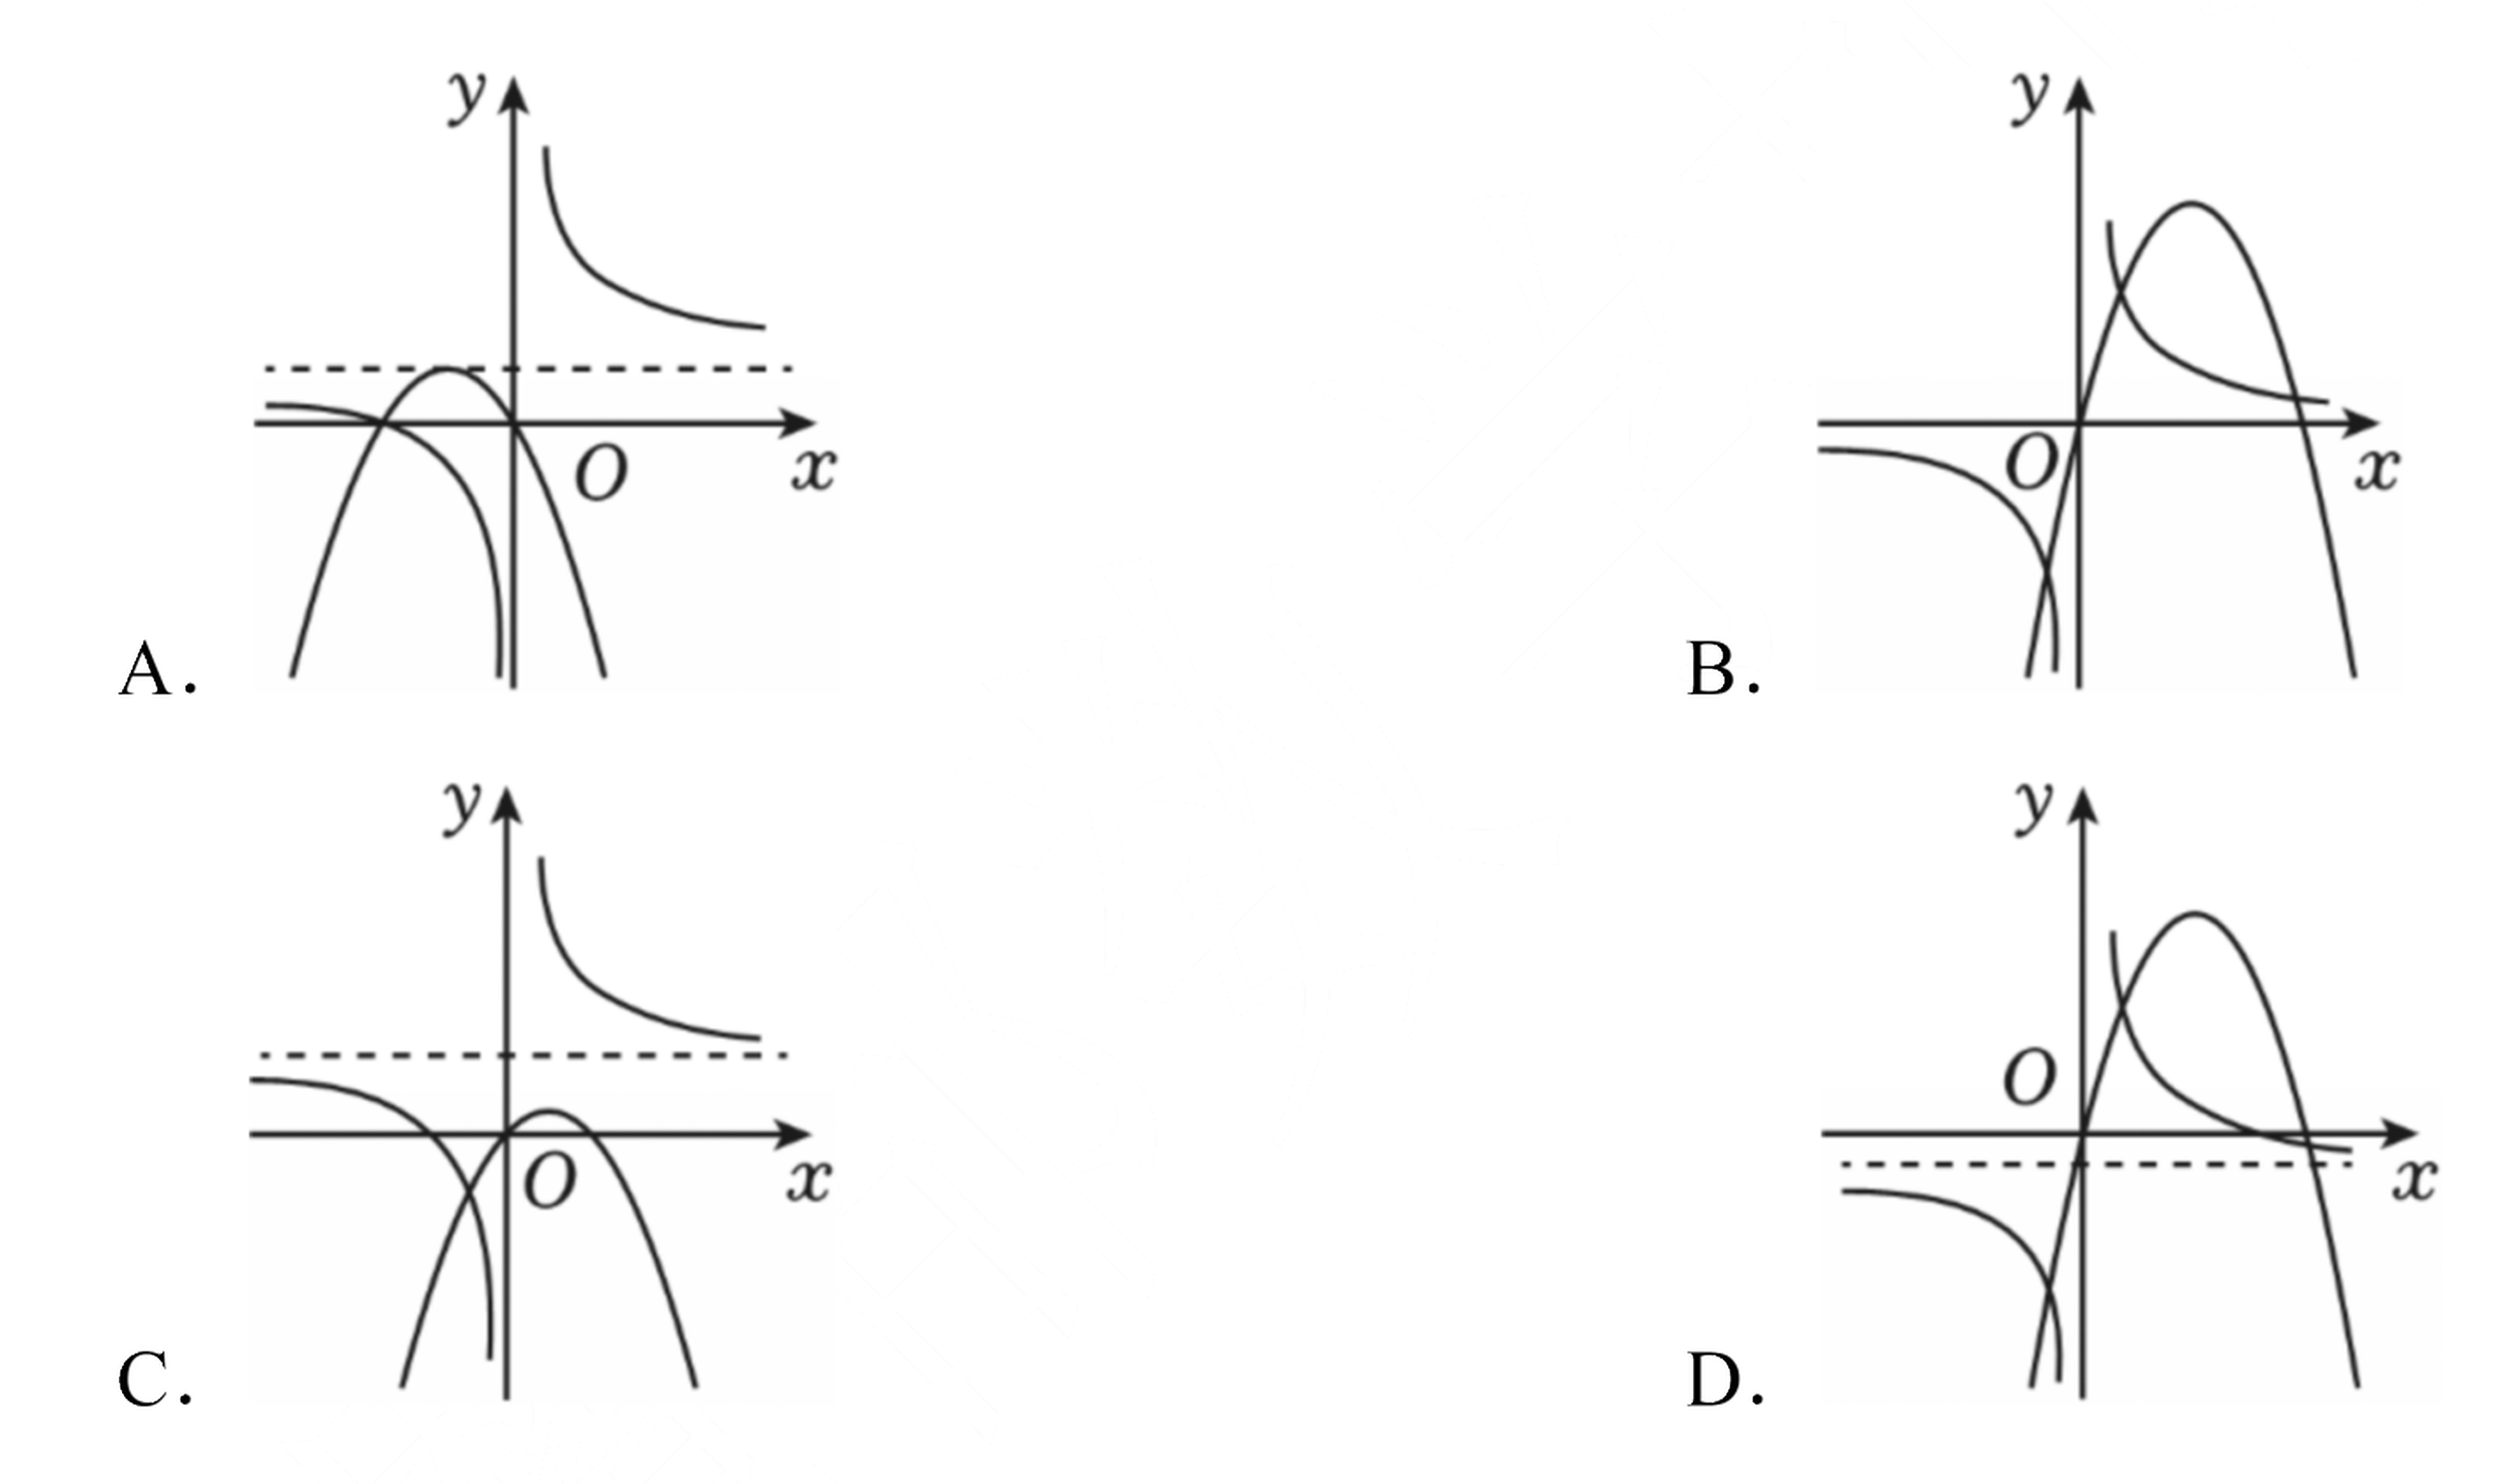
\includegraphics[width=0.80\textwidth]{figures/gao161_q14.png}
\end{center}

\ifanswer
\solbegin
\step{$A$ 选项，由二次函数图象得 $a<0$，$b<0$，由幂函数型函数图象得 $a<0$，$b>0$，}
\step{故 $A$ 选项错误；}
\step{$B$ 选项，由二次函数图象得 $a<0$，$b>0$，由幂函数型函数图象得 $a<0$，$b=0$，}
\step{故 $B$ 选项错误；}
\step{$C$ 选项，由二次函数图象得 $a<0$，$b>0$，由幂函数型函数图象得 $a<0$，$b>0$，}
\step{故 $C$ 选项正确；}
\step{$D$ 选项，由二次函数图象得 $a<0$，$b>0$，由幂函数型函数图象得 $a<0$，$b<0$，}
\step{故 $D$ 选项错误.}
\step{故选 $C$.}
\solend
\fi

% === Q15 === \subseteq／\subset、\varnothing、\mid；"排除 C""排除 B、D"正体字母照录；解析 4 行，故选 $A$
\item 设不等式 $\lvert f(x)\rvert+\lvert g(x)\rvert<a$（常数 $a>0$）的解集是 $M$，设不等式 $\lvert f(x)+g(x)\rvert<a$（常数 $a>0$）的解集是 $N$，则\mbox{（\quad）}

\keepwithprev
A. $M\subseteq N$\qquad B. $N\subseteq M$\qquad C. $M\subset N$\qquad D. $N\subset M$

\ifanswer
\solbegin
\step{$x\in M\Rightarrow\lvert f(x)+g(x)\rvert\leqslant\lvert f(x)\rvert+\lvert g(x)\rvert<a\Rightarrow x\in N$，所以 $M\subseteq N$.}
\step{取 $f(x)=g(x)=0$，则 $M=N$，排除 C.}
\step{取 $f(x)=1$，$g(x)=-1$，$a=1$，则 $M=\varnothing$，$N$ 为全体实数，排除 B、D.}
\step{故选 $A$.}
\solend
\fi

% === Q16 === "人文集"定义证明；cases 无；解析 21 行，故选 $B$
\item 设集合 $I_n=\{1,2,\cdots,n\}$，$n\in\N,n\geqslant1$，集合 $P_n=\left\{\dfrac{m}{\sqrt k}\mid m\in I_n,k\in I_n\right\}$，若 $P_n$ 的子集 $A$ 中任意两个元素之和不是整数的平方，则称 $A$ 为 “人文集”. 那么使 $P_n$ 能分成两个交集为空集的 “人文集” 的并集，且这两个人文集的并集恰为 $P_n$ 时，$n$ 的最大值是\mbox{（\quad）}

\keepwithprev
A. 13\qquad B. 14\qquad C. 15\qquad D. 16

\ifanswer
\solbegin
\step{先证当 $n\geqslant15$ 时，$P_n$ 不能分成两个不相交的人文集的并集.}
\step{假设当 $n\geqslant15$ 时，$P_n$ 可以分成两个不相交的人文集的并集，}
\step{设 $A$ 和 $B$ 为两个不相交的人文集，使 $A\cup B=P_n\supseteq I_n$.}
\step{不妨设 $1\in A$，则由于 $1+3=2^2$，所以 $3\notin A$，即 $3\in B$.}
\step{同理可得，$6\in A$，$10\in B$. 又推出 $15\in A$，}
\step{但 $1+15=4^2$，这与 $A$ 为人文集相矛盾.}
\step{再证 $P_{14}$ 满足要求. 当 $k=1$ 时，$P_{14}=\left\{\dfrac{m}{\sqrt k}\mid m\in I_{14},k\in I_{14}\right\}$，}
\step{可以分成 2 个人文集的并集.}
\step{事实上，只要取 $A_1=\{1,2,4,6,9,11,13\}$，$B_1=\{3,5,7,8,10,12,14\}$，}
\step{则 $A_1$ 和 $B_1$ 都是人文集，且 $A_1\cup B_1=P_{14}$.}
\step{当 $k=4$ 时，集合 $\left\{\dfrac{m}{\sqrt k}\mid m\in I_{14}\right\}$ 中，除整数外，}
\step{剩下的数组成集合 $\left\{\dfrac12,\dfrac32,\dfrac52,\cdots,\dfrac{13}{2}\right\}$，}
\step{可以分为下列 2 个人文集的并：$A_2=\left\{\dfrac12,\dfrac52,\dfrac92,\dfrac{11}{2}\right\}$，$B_2=\left\{\dfrac32,\dfrac72,\dfrac{13}{2}\right\}$.}
\step{当 $k=9$ 时，集合 $\left\{\dfrac{m}{\sqrt k}\mid m\in I_{14}\right\}$ 中，除整数外，}
\step{剩下的数组成集合 $\left\{\dfrac13,\dfrac23,\dfrac43,\dfrac53,\cdots,\dfrac{13}{3},\dfrac{14}{3}\right\}$，}
\step{可以分为下列 2 个人文集的并：$A_3=\left\{\dfrac13,\dfrac43,\dfrac53,\dfrac{10}{3},\dfrac{13}{3}\right\}$，$B_3=\left\{\dfrac23,\dfrac73,\dfrac83,\dfrac{11}{3},\dfrac{14}{3}\right\}$.}
\step{最后，集合 $C=\left\{\dfrac{m}{\sqrt k}\mid m\in I_{14},k\in I_{14},k\ne1,4,9\right\}$ 中的数的分母都是无理数，}
\step{它与 $P_n$ 中的任何其他数之和都不是整数，}
\step{因此，令 $A=A_1\cup A_2\cup A_3\cup C$，$B=B_1\cup B_2\cup B_3$，}
\step{则 $A$ 和 $B$ 是不相交的人文集，且 $A\cup B=P_{14}$.}
\step{综上，$n$ 的最大值为 14，故选 $B$.}
\solend
\fi

\end{enumerate}

\bigsec{三、解答题}

\begin{enumerate}
\setcounter{enumi}{16}

% === Q17 === "图像"照录；\Z；cases 块；解析 9 行，跨 06—07 页
\item (1) 已知函数 $y=x^{\frac{4m-m^2}{2}}$（$m\in\Z$）在区间 $(0,+\infty)$ 上是严格增函数，它的图像关于 $y$ 轴对称，求 $m$ 的值及该函数的解析式；

(2) 若 $(a-2)^{\frac32}<(1+2a)^{\frac32}$，求实数 $a$ 的取值范围.

\ifanswer
\solbegin
\step{(1) 由幂函数在 $(0,+\infty)$ 上严格递增，得 $\dfrac{4m-m^2}{2}>0\Leftrightarrow0<m<4$，}
\step{又 $m\in\Z$，所以 $m\in\{1,2,3\}$.}
\step{当 $m=1$ 或 $m=3$ 时，函数为 $y=x^{\frac32}$，定义域为 $[0,+\infty)$，}
\step{图像不关于 $y$ 轴对称.}
\step{当 $m=2$ 时，函数为 $y=x^2$，满足题意，所以 $m=2$，解析式 $y=x^2$.}
\step{(2) 原不等式有意义，须满足 $\begin{cases}a-2\geqslant0\\1+2a\geqslant0\end{cases}\Leftrightarrow a\geqslant2$，}
\step{函数 $y=x^{\frac32}$ 在 $[0,+\infty)$ 上严格递增，}
\step{因此 $(a-2)^{\frac32}<(1+2a)^{\frac32}\Leftrightarrow a-2<1+2a\Leftrightarrow a>-3$，}
\step{结合 $a\geqslant2$，得 $a\in[2,+\infty)$.}
\solend
\fi

% === Q18 === 题干"$a\geqslant0$"与解析"$a<0$"自相矛盾照录；"$A\cap B=(-2,-1]\cap[2,6)$"误印 ∩ 照录；\subseteq；解析 10 行
\item 已知实数 $a\geqslant0$，集合 $A=\left\{x\mid\dfrac{x+2}{x-6}<0\right\}$，$B=\{x\mid\lvert2x-1\rvert\geqslant3\}$，$C=\{x\mid x^2-3ax+2a^2<0\}$，

(1) 求 $A\cap B$；

(2) 若 $C\subseteq(A\cap B)$，求 $a$ 的取值范围.

\ifanswer
\solbegin
\step{(1) 由 $\dfrac{x+2}{x-6}<0$ 得 $-2<x<6$，即 $A=\{x\mid-2<x<6\}=(-2,6)$，}
\step{由 $\lvert2x-1\rvert\geqslant3$ 得 $2x-1\geqslant3$ 或 $2x-1\leqslant-3$，解得 $x\geqslant2$ 或 $x\leqslant-1$，}
\step{即 $B=(-\infty,-1]\cup[2,+\infty)$，}
\step{所以 $A\cap B=(-2,-1]\cap[2,6)$；}% 原卷把 ∪ 误印成 ∩，照录未改（见 ⑤ 2）
\step{(2) 由 (1) 得 $A\cap B=\{x\mid-2<x\leqslant-1\text{ 或 }2\leqslant x<6\}$，}
\step{因为 $C\subseteq(A\cap B)$，$x^2-3ax+2a^2=(x-a)(x-2a)<0$，}% 题干 $a\geqslant0$ 与解析 $a<0$ 自相矛盾，照录未改（见 ⑤ 1）
\step{当 $a=0$ 时，$C=\varnothing$，符合题意；}
\step{当 $a>0$ 时，$C=(a,2a)$，则 $\begin{cases}a\geqslant2\\2a\leqslant6\\a>0\end{cases}$，解得 $2\leqslant a\leqslant3$，}
\step{当 $a<0$ 时，$C=(2a,a)$，则 $\begin{cases}2a\geqslant-2\\a\leqslant-1\\a<0\end{cases}$，解得 $a=-1$，}
\step{故 $a$ 的范围为 $\{-1,0\}\cup[2,3]$.}
\solend
\fi

% === Q19 === 双碳太阳能应用题；"双碳""自发自用、市电互补"弯引号；解析 8 行，跨 08 页上下
\item 为响应 “双碳” 目标，某电子企业拟安装一套可使用 10 年的太阳能供电设备. 该设备的安装费用 $P(x)$（单位：万元）与太阳能电池板面积 $x(x>0)$（单位：平方米）成正比，比例系数为 $\dfrac12$. 为保障生产用电，安装后采用 “自发自用、市电互补” 模式，在此模式下，企业每年消耗的电费 $Q(x)$（单位：万元）与安装的这种太阳能电池板的面积 $x$ 之间的函数关系是 $Q(x)=\dfrac{180}{x+5}$. 记 $W(x)$（单位：万元）为该企业安装这种太阳能供电设备的费用与 10 年所消耗的电费之和.

(1) 要使该设备的安装费与第 1 年的电费之和不超过 17 万元，求安装太阳能电池板面积 $x$ 的取值范围；

(2) 当 $x$ 为多少平方米时，$W(x)$ 取得最小值？最小值是多少万元？

\ifanswer
\solbegin
\step{(1) $P(x)=\dfrac{x}{2}$，安装费与第 1 年的电费之和不超过 17 万元，即 $\dfrac{x}{2}+\dfrac{180}{x+5}\leqslant17$，}
\step{$x>0$，上式等价于 $x^2-29x+190\leqslant0\Leftrightarrow(x-10)(x-19)\leqslant0$，}
\step{解得 $x\in[10,19]$.}
\step{(2) 安装费用与 10 年电费之和为 $W(x)=P(x)+10Q(x)$，}
\step{$=\dfrac{x}{2}+\dfrac{1800}{x+5}=\dfrac{x+5}{2}+\dfrac{1800}{x+5}-\dfrac52$，}
\step{$x>0$，由基本不等式得 $W(x)\geqslant2\sqrt{\dfrac{x+5}{2}\cdot\dfrac{1800}{x+5}}-\dfrac52=60-\dfrac52=57.5$，}
\step{等号当且仅当 $\dfrac{x+5}{2}=\dfrac{1800}{x+5}$，即 $x=55$ 时成立.}
\step{因此，当电池板面积为 55 平方米时，$W(x)$ 取得最小值 57.5 万元.}
\solend
\fi

% === Q20 === $a*b$ 定义；\min 改正体；cases 块；解析 23 行，跨 08—10 页
\item 设 $a$、$b\in\R$，定义 $a*b=\begin{cases}a,&a<b\\b,&a\geqslant b\end{cases}$.

(1) 若 $x*2>1$，求 $x$ 的取值范围；

(2) 若 $(\lvert x-1\rvert+\lvert x-2\rvert)*3=3$，求 $x$ 的取值范围；

(3) 若 $a$、$b>0$，记 $M=a*\dfrac{b}{a^2+4b^2}$，分别比较 $M$ 与 $a$，以及 $M$ 与 $\dfrac{b}{a^2+4b^2}$ 的大小，并求 $M$ 的最大值.

\ifanswer
\solbegin
\step{(1) 定义 $a*b=\begin{cases}a,&a<b\\b,&a\geqslant b\end{cases}$，由 $x*2>1$，得 $\begin{cases}x<2\\x>1\end{cases}$，或 $\begin{cases}x\geqslant2\\2>1\end{cases}$，}
\step{解得 $x>1$，即 $x$ 的取值范围为 $\{x\mid x>1\}$；}
\step{(2) 当 $x\geqslant2$ 时，$\lvert x-1\rvert+\lvert x-2\rvert=2x-3\geqslant1$，}
\step{当 $1\leqslant2x-3\leqslant3$，即 $2\leqslant x\leqslant3$ 时，}
\step{此时 $(\lvert x-1\rvert+\lvert x-2\rvert)*3=2x-3=3$，解得 $x=3$；}
\step{当 $2x-3>3$，即 $x>3$ 时，}
\step{此时 $(\lvert x-1\rvert+\lvert x-2\rvert)*3=3$ 恒成立，则 $x>3$；}
\step{当 $-2x+3>3$，即 $x<0$ 时，}
\step{此时 $(\lvert x-1\rvert+\lvert x-2\rvert)*3=3$ 恒成立，则 $x<0$.}
\step{当 $1<x<2$ 时，$\lvert x-1\rvert+\lvert x-2\rvert=1$，}
\step{此时 $(\lvert x-1\rvert+\lvert x-2\rvert)*3=1\ne3$，不符合题意；}
\step{当 $x\leqslant1$ 时，$\lvert x-1\rvert+\lvert x-2\rvert=-2x+3\geqslant1$，}
\step{当 $-2x+3\leqslant3$，即 $0\leqslant x\leqslant1$ 时，}
\step{此时 $(\lvert x-1\rvert+\lvert x-2\rvert)*3=-2x+3=3$，解得 $x=0$.}
\step{综上所述，$x$ 的取值范围为 $\{x\mid x\leqslant0\text{ 或 }x\geqslant3\}$；}
\step{(3) 由题意，$M=a*\dfrac{b}{a^2+4b^2}=\min\left\{a,\dfrac{b}{a^2+4b^2}\right\}$，}% 原卷印斜体 min，按全稿惯例改正体 \min（见 ② ⑬）
\step{则 $M\leqslant a$，$M\leqslant\dfrac{b}{a^2+4b^2}$.}
\step{因为 $a$、$b>0$，所以 $\dfrac{b}{a^2+4b^2}\leqslant\dfrac{b}{2\sqrt{a^2\cdot4b^2}}=\dfrac{1}{4a}$，}
\step{当且仅当 $a=2b>0$ 时取等号，}
\step{当 $a\geqslant\dfrac{1}{4a}$，即 $a\geqslant\dfrac12$ 时，$M=a*\dfrac{b}{a^2+4b^2}=\dfrac{b}{a^2+4b^2}\leqslant\dfrac{1}{4a}$，}
\step{则 $a=\dfrac12$，$b=\dfrac14$ 时，$M$ 取得最大值 $\dfrac12$；}
\step{当 $0<a<\dfrac12$ 时，$M=a*\dfrac{b}{a^2+4b^2}=a$，此时 $M<\dfrac12$.}
\step{综上所述，$M$ 的最大值为 $\dfrac12$.}
\solend
\fi

% === Q21 === $A_n$／$B_n$／$S_n$／$T_n$ 新定义；题干第 3 问误标 (2) 照录、解析作 (3)；\prec；解析 25 行，跨 10—11 页
\item 对任意正整数 $n$，记集合 $A_n=\{(a_1,a_2,\cdots,a_n)\mid a_1,a_2,\cdots,a_n$ 均为非负整数，且 $a_1+a_2+\cdots+a_n=n\}$，集合 $B_n=\{(b_1,b_2,\cdots,b_n)\mid b_1,b_2,\cdots,b_n$ 均为非负整数，且 $b_1+b_2+\cdots+b_n=2n\}$. 设 $\alpha=(a_1,a_2,\cdots,a_n)\in A_n$，$\beta=(b_1,b_2,\cdots,b_n)\in B_n$，若对任意 $i\in\{1,2,\cdots,n\}$ 都有 $a_i\leqslant b_i$，则记 $\alpha\prec\beta$.

(1) 写出集合 $A_2$ 和 $B_2$；

(2) 证明：对任意 $\alpha\in A_n$，存在 $\beta\in B_n$，使得 $\alpha\prec\beta$；

(2) 设集合 $S_n=\{(\alpha,\beta)\mid\alpha\in A_n,\beta\in B_n,\alpha\prec\beta\}$，求证：$S_n$ 中的元素个数是完全平方数.% 原卷第 3 问题干误标 (2)（与第 2 问重号），照录未改（见 ⑤ 3）

\ifanswer
\solbegin
\step{(1) $A_2=\{(0,2),(1,1),(2,0)\}$，$B_2=\{(0,4),(1,3),(2,2),(3,1),(4,0)\}$；}
\step{(2) 对任意 $\alpha=(a_1,a_2,\cdots,a_n)\in A_n$，设 $b_i=a_i+1$（$i=1,2,3,\cdots,n$），}
\step{则 $b_1,b_2,\cdots,b_n$ 均为非负整数，且 $a_i\leqslant b_i$（$i=1,2,3,\cdots,n$）.}
\step{令 $\beta=(b_1,b_2,\cdots,b_n)$，则 $b_1+b_2+\cdots+b_n$}
\step{$=(a_1+1)+(a_2+1)+\cdots+(a_n+1)=(a_1+a_2+\cdots+a_n)+n=2n$，}
\step{所以 $\beta\in B_n$，且 $\alpha\prec\beta$.}
\step{(3) 对任意 $\alpha=(a_1,a_2,\cdots,a_n)\in A_n$，$\alpha'=(a_1',a_2',\cdots,a_n')\in A_n$，}
\step{记 $\alpha+\alpha'=(a_1+a_1',a_2+a_2',\cdots,a_n+a_n')$，}
\step{则 $a_1+a_1',a_2+a_2',\cdots,a_n+a_n'$ 均为非负整数，}
\step{且 $(a_1+a_1')+(a_2+a_2')+\cdots+(a_n+a_n')$}
\step{$=(a_1+a_2+\cdots+a_n)+(a_1'+a_2'+\cdots+a_n')=n+n=2n$，}
\step{所以 $\alpha+\alpha'\in B_n$，且 $\alpha\prec\alpha+\alpha'$，$\alpha'\prec\alpha+\alpha'$.}
\step{设集合 $A_n$ 中的元素个数为 $t$，设 $A_n=\{\alpha_1,\alpha_2,\cdots,\alpha_t\}$.}
\step{设集合 $T_n=\{(\alpha_i,\alpha_i+\alpha_j)\mid i=1,2,\cdots,t,j=1,2,\cdots,t\}$.}
\step{对任意 $\alpha_i\in A_n$（$i=1,2,\cdots,t$），都有 $\alpha_i+\alpha_1,\alpha_i+\alpha_2,\cdots,\alpha_i+\alpha_t\in B_n$，}
\step{且 $\alpha_i\prec\alpha_i+\alpha_j$，$j=1,2,\cdots,t$，所以 $T_n\subseteq S_n$.}
\step{若 $(\alpha,\beta)\in S_n$，其中 $\alpha=(a_1,a_2,\cdots,a_n)\in A_n$，$\beta=(b_1,b_2,\cdots,b_n)\in B_n$，}
\step{设 $c_i=b_i-a_i$（$i=1,2,\cdots,n$），因为 $a_i\leqslant b_i$，所以 $c_i=b_i-a_i\geqslant0$，}
\step{记 $\alpha'=(c_1,c_2,\cdots,c_n)$，}
\step{则 $c_1+c_2+\cdots+c_n=(b_1-a_1)+(b_2-a_2)+\cdots+(b_n-a_n)$}
\step{$=(b_1+b_2+\cdots+b_n)-(a_1+a_2+\cdots+a_n)=2n-n=n$，}
\step{所以 $\alpha'\in A_n$，并且有 $\beta=\alpha+\alpha'$，所以 $(\alpha,\beta)\in T_n$，所以 $S_n\subseteq T_n$，}
\step{所以 $S_n=T_n$.}
\step{因为集合 $T_n$ 中的元素个数为 $t^2$，所以 $S_n$ 中的元素个数为 $t^2$，}
\step{是完全平方数.}
\solend
\fi

\end{enumerate}

\end{document}
"
% 紧凑版：xelatex "\def\iscompact{1}% 高一161_松江一中嘉一实验_期中.tex
%   —— 高一上数学"2026-2027 年松江一中嘉一实验高一上期中"（试卷版/答案版/紧凑版）
% 试卷版：xelatex 高一161_松江一中嘉一实验_期中.tex
% 答案版：xelatex "\def\isanswer{1}% 高一161_松江一中嘉一实验_期中.tex
%   —— 高一上数学"2026-2027 年松江一中嘉一实验高一上期中"（试卷版/答案版/紧凑版）
% 试卷版：xelatex 高一161_松江一中嘉一实验_期中.tex
% 答案版：xelatex "\def\isanswer{1}% 高一161_松江一中嘉一实验_期中.tex
%   —— 高一上数学"2026-2027 年松江一中嘉一实验高一上期中"（试卷版/答案版/紧凑版）
% 试卷版：xelatex 高一161_松江一中嘉一实验_期中.tex
% 答案版：xelatex "\def\isanswer{1}\input{高一161_松江一中嘉一实验_期中.tex}"
% 紧凑版：xelatex "\def\iscompact{1}\input{高一161_松江一中嘉一实验_期中.tex}"
%
% ① 原始材料：微信公众号"魔都数学加油站"文章，连载"27学年高一161"，原卷卷面标题
% "2026-2027 年松江一中嘉一实验高一上期中"（卷面未印副标题、未印连载号）。
% 正文为 11 张 PNG 页（01/02/03/05/06/07/08/09/11 为 4762×6735，04/10 为
% 2560×3620，同一篇各页分辨率混排，逐页按各自分辨率裁图核对）。
% 体例：讲评版——填空 3—12（10 题）、选择 13—16（4 题）、解答 17—21（5 题），
% 共 19 题，自第 3 题起编（1、2 未印在本篇）；Q13 答案"A"直接印在题干括号内、
% 且无【答案】/【解析】段，本稿按 高一37 第 13 题／高一57 第 13 题成例把括号
% 留空、另提 \ans{$A$}；其余 18 题逐题印【解析】、用 \solbegin…\solend。
% 题目、答案、解析均据原图转录；卷面粉红色水印"魔都数学加油站"及公众号页脚未录入。
% 全卷插图清单（逐页通读 11 页确认）：仅 1 组——Q14 四幅图像选项（04 页 2×2
% 排布，二次函数与幂函数型函数在同一坐标系中的图象，A/B/C/D 四幅小图），
% 合并成一张，三版都出，裁 figures/gao161_q14.png。其余各页逐页确认无其它
% 题目配图、无解析内配图、无表格、无"如图"处（Q16 解析里的"可以分为下列 2 个
% 人文集的并"是纯文字＋集合，不是表格；OCR 里看似表格的行实为大括号与分数）。
%
% 卷首标题：原卷印作"2026-2027 年松江一中嘉一实验高一上期中"，年份区间按全稿惯例排 en dash；
% 原卷卷面未印副标题，本稿按同期中卷知识模块口径补出"集合与常用逻辑用语、不等式、函数"。
%
% ② 与原卷的排版差异／照录项清单：
%   ① 原文从第 3 题起，本稿保留原题号；共 19 题三节，解答题 5 题到 21；
%      三节各自一个 enumerate + \setcounter{enumi}{2}/{12}/{16}（不贯穿），
%      用 \examtitlest[3] 起手；
%   ② 混合体例：Q13 原卷把答案"A"直接印在题干括号内（"（  A  ）"）、且题下
%      无【答案】/【解析】段，按 高一37 第 13 题／高一57 第 13 题成例把括号
%      留空、另提 \ans{$A$}、不补造解析；其余 18 题印【解析】、用
%      \solbegin…\solend；四道选择题中 Q14/Q15/Q16 的答案在解析末句
%      "故选 $C$／$A$／$B$"、Q13 用 \ans{$A$}；括号 \mbox{（\quad）} 留空；
%      答案版【答案】/【解析】标记数 = 19 = 全卷题数（1 个 \ans ＋ 18 个 \solbegin）；
%   ③ 原卷卷面未印副标题，本稿按知识模块口径补出；
%   ④ 原卷填空横线按全稿惯例排 \blankline[4.4em]；选择题选项段前按惯例各加
%      \keepwithprev；Q14 四幅选项图整块用 \needvspace{9cm} 守卫（守卫放
%      \item 之前，见 高一132 Q14／高一154 Q15 成例）；解答题不留作答区、
%      不加 \anspace（原卷为讲评版）；
%   ⑤ 数集归一：Q8"$x\in\R$"、Q11"$m\in\R$"、Q13"$x,y\in\N$"、
%      Q16"$n\in N$"、Q17"$m\in\Z$"、Q20"$a$、$b\in R$"——原卷印正体粗体
%      或斜体 R/N/Z，按全稿惯例归一 \R／\N／\Z；绝对值排 \lvert…\rvert
%      （Q9、Q12、Q15、Q18、Q20），集合描述竖线排 \mid（Q12、Q16、Q18、
%      Q20、Q21），空集 \varnothing（Q15、Q18），补集无用例，不等号按全稿
%      惯例排 \leqslant／\geqslant；
%   ⑥ 子集符号逐处照录不统一：Q12 cases 定义"$C(A)\geqslant C(B)$"、
%      Q15 选项 A/B"$M\subseteq N$""$N\subseteq M$"与解析"$M\subseteq N$"
%      印带下划线 ⊆（照录 \subseteq），Q15 选项 C/D"$M\subset N$""$N\subset M$"
%      印单线 ⊂（照录 \subset），Q18 "$C\subseteq(A\cap B)$"、Q21
%      "$T_n\subseteq S_n$""$S_n\subseteq T_n$"均带下划线照录 \subseteq；
%      本卷无 \not\subset 用例；
%   ⑦ 判别式：Q7 解析"$\Delta=(m-6)(m+2)>0$"、Q8 解析"$\Delta=a^2-4a<0$"、
%      Q12 解析"$\Delta=a^2-8$"共 3 处，逐处放大确认印等腰偏高粗三角
%      （高>宽、右斜边粗），照录 \Delta；本卷无扁等边细线 \triangle 用例；
%   ⑧ 中文弯引号照录：Q7"$m\geqslant6$""有两个不相等的正实数根"及四个
%      条件短语、Q13 反证法命题、Q16"人文集"、Q19"双碳""自发自用、市电互补"；
%      注释里一律 ASCII 引号；数学式内 CJK 用 \text{}（Q18、Q20 解集描述内"或"）；
%   ⑨ "图像／图象"逐处照录不统一：Q4"的图像"、Q17 题干"它的图像关于 $y$ 轴
%      对称"及解析"图像不关于 $y$ 轴对称"印"图像"；Q14 题干"的图象可能为"
%      与解析 A/B/C/D 四行各"由二次函数图象得""由幂函数型函数图象得"
%      共 8 处印"图象"（象，无亻）；
%   ⑩ 文本圈数字逐处照录：Q12 题干①②③④、Q12 解析"故①错误""故②正确"
%      "故③正确""故④错误""故正确的是②③"，均为印刷圈数字（文本模式）；
%   ⑪ 半角逗号在数学组之间是全稿惯例、非笔误，逐处照录（Q5"$a$、$b$"、
%      Q13"$x,y\in\N$"、Q16"$n\in\N,n\geqslant1$"与集合描述内逗号、
%      Q20"$a,b\in\R$"、Q21 各集合描述内逗号）；行末西文句点 ASCII `.`；
%      原卷行中句点（Q16"$10\in B$. 又推出 $15\in A$"、Q16"再证 $P_{14}$
%      满足要求. 当 $k=1$ 时"、Q18"$A\cap B=(-2,-1]\cap[2,6)$；"后的分号）
%      按全稿惯例一律排 ASCII `.`／全角"；"；中文语境行中全角逗号／顿号照录；
%   ⑫ 原卷数学式内联条件（Q14"$y=x^a+b(a\ne0)$"、Q19"$x(x>0)$"、
%      Q11"$\lvert x-m\rvert<n\,(m\in\R,n>0)$"）印半角括号，逐处照录未改
%      全角（同 高一147 口径）；
%      中文语境的括注（Q5"结果用 $a$、$b$ 表示"、Q7"填…"、Q12"填写序号"、
%      Q15"常数 $a>0$"、Q19"单位：万元"）印全角括号，照录；
%   ⑬ 复杂式照录别简化：Q3 $(a^{2-\sqrt3})^{2+\sqrt3}\times\sqrt{a^2}\times
%      b^{\sqrt3}\times b^{1-\sqrt3}$ 与 $a^{(2-\sqrt3)(2+\sqrt3)}\cdot a\cdot
%      b^{\sqrt3+1-\sqrt3}=a\cdot a\cdot b=a^2b$（题干用 \times、解析用 \cdot，
%      逐处照录不统一，见 ⑤）；Q5 $\dfrac{\lg2}{\lg2+\lg3}=\dfrac{a}{a+b}$、
%      Q10 $t-\dfrac3t=2$ 与 $b=a^3$、$ab=a^4=2$、Q11 $\left(2a-\dfrac12
%      -a+\dfrac12,2a-\dfrac12+a-\dfrac12\right)=(a,3a-1)$ 与
%      $\left(\dfrac43,\dfrac53\right]\cup\{2\}$、Q16 各分数集合、Q19
%      $x^2-29x+190\leqslant0$ 与 $W(x)=P(x)+10Q(x)$ 与
%      $2\sqrt{\dfrac{x+5}{2}\cdot\dfrac{1800}{x+5}}-\dfrac52=60-\dfrac52=57.5$、
%      Q20 $M=a*\dfrac{b}{a^2+4b^2}=\min\left\{a,\dfrac{b}{a^2+4b^2}\right\}$
%      与 $\dfrac{b}{2\sqrt{a^2\cdot4b^2}}=\dfrac{1}{4a}$、Q21 各 $A_n$／$B_n$／
%      $T_n$ 定义；\left…\right 不得拆到不同 $…$ 组（Q11 的 \left(…\right)、
%      Q11 的 \left(\dfrac43,\dfrac53\right]、Q16 的 \left\{\dfrac{m}{\sqrt k}
%      \mid…\right\} 与 \left\{\dfrac12,\dfrac32,\dfrac52,\cdots,\dfrac{13}{2}\right\}
%      等、Q20 的 \min\left\{…\right\}）；cases 块整体算一个印刷行
%      （Q12 定义、Q17 (2)、Q18 (2) 两处、Q20 定义与 (1)）；原卷 Q20 解析
%      "$=min\{…\}$"印斜体 min，按 高一122／高一102 成例改正体 \min；
%   ⑭ 一条 \step = 原卷解析的一个印刷行；别并折行、别拆行。跨页续印按题合并
%      （Q6 的 01 页上下题干重复印、Q10 的 01—02 页、Q11 的 02—03 页、
%      Q12 的 03—04 页、Q16 的 05—06 页、Q17 的 06—07 页、Q18 的 07 页
%      上下、Q19 的 08 页上下、Q20 的 08—10 页、Q21 的 10—11 页）；
%      跨半页重叠行（Q10"令 $t=\log_a b>0$…"、Q16"它与 $P_n$ 中的任何
%      其他数之和都不是整数，"、Q18"【解析】(1) 由 $\dfrac{x+2}{x-6}<0$…"、
%      Q19"$x>0$，上式等价于…"、Q20"此时…则 $x<0$."、Q21"若 $(\alpha,\beta)
%      \in S_n$…"与"设 $c_i=b_i-a_i$…"）只算一个印刷行；
%   ⑮ 自定义记号照录：Q12"$C(A)$""$A*B$""$S$"、Q16"$I_n$""$P_n$""人文集"
%      "$A_1$／$B_1$／$A_2$／$B_2$／$A_3$／$B_3$／$C$"、Q20"$a*b$""$M$"、
%      Q21"$A_n$／$B_n$／$S_n$／$T_n$""$\alpha\prec\beta$""$\alpha+\alpha'$"；
%   ⑯ 选项字母体例照录不统一：Q15 解析"排除 C.""排除 B、D."两处原卷印
%      正体（文本模式），Q13 \ans{$A$}、Q14"$A$ 选项"…"故选 $C$"、
%      Q15"故选 $A$"、Q16"故选 $B$"用斜体（数学模式），逐处照录、不统一；
%   ⑰ 红字：全卷逐页扫描无红色加粗小标题（仅粉色水印），故本卷无 \stepm，
%      不引入红色定义；
%
% ③ 行数复核：一条 \step = 原卷解析的一个印刷行，cases 块作一个印刷行计。
%   逐题数（逐页核对定稿）：Q3：1；Q4：1；Q5：1；Q6：3；Q7：4；Q8：4；
%   Q9：2；Q10：2；Q11：7；Q12：8；Q13：0（答案印括号内、提 \ans{}，
%   不计入 \step 账）；Q14：9；Q15：4；Q16：21；Q17：9；Q18：10；Q19：8；
%   Q20：23；Q21：25。
%   合计 142 行（142 条 \step，无 \stepm），与原卷逐题印刷行相等。
%   全卷 19 题：Q13 一处 \ans{} ＋ 其余 18 题设 \solbegin…\solend，
%   答案版【答案】/【解析】标记数 = 19 = 全卷题数。
%
% ④ 页码分布（供回原图复核）：
%   卷首标题＋"一、填空题"＋Q3/Q4/Q5 题干＋解析各 1 行＋Q6 题干首行
%   在 01 页上半；Q6 题干（重复印）＋解析 3 行＋Q7 题干＋解析 4 行在
%   01 页下半；Q8 题干＋解析 4 行＋Q9 题干＋解析 2 行＋Q10 题干＋
%   解析首行在 02 页上半；Q10 解析（重复印）＋末行＋Q11 题干＋解析
%   前 3 行在 02 页下半；Q11 解析后 4 行＋Q12 题干＋cases 定义＋①
%   在 03 页上半；Q12 ②③④ 三命题＋"填写序号"行＋解析前 6 行在
%   03 页下半；Q12 解析后 2 行＋"二、选择题"标题＋Q13 题干＋选项＋
%   Q14 题干＋"（　）"＋A/B 两幅图在 04 页上半；Q14 四幅图（重复印）
%   ＋解析 9 行在 04 页下半；Q15 题干＋选项＋解析 4 行＋Q16 题干＋
%   选项在 05 页上半；Q16 题干（重复印）＋选项＋解析前 10 行在 05 页
%   下半；Q16 解析中 8 行（k=4、k=9 两批＋集合 C＋"它与 $P_n$…"）
%   在 06 页上半；Q16 解析"它与 $P_n$…"（重复印）＋末 3 行＋
%   "三、解答题"标题＋Q17 题干＋两问＋解析前 4 行在 06 页下半；
%   Q17 解析后 5 行＋Q18 题干＋两问＋解析首行在 07 页上半；Q18 解析
%   （重复首行）＋余 9 行在 07 页下半；Q19 题干＋两问＋解析前 2 行在
%   08 页上半；Q19 解析（重复第 2 行）＋余 6 行＋Q20 定义＋(1) 问在
%   08 页下半；Q20 (2)(3) 两问＋解析 (1) 2 行＋(2) 前 7 行在 09 页
%   上半；Q20 解析 (2) 余 4 行＋(3) 前 4 行在 09 页下半；Q20 解析 (3)
%   余 4 行＋Q21 题干＋三问在 10 页上半；Q21 题干（重复印）＋解析
%   (1)(2)(3) 前 8 行在 10 页下半；Q21 解析 (3) 中 10 行在 11 页上半；
%   Q21 解析 (3)（重复 2 行）＋末 7 行"是完全平方数."在 11 页下半。
%   本稿按题连排，不丢行、不并折行；全卷末题为第 21 题，无附加题节。
%
% ⑤ 存疑照录（放大原图确认，照录未改、正文对应处另有 % 注）：
%   1. Q18 题干印"已知实数 $a\geqslant0$"，解析却另设"当 $a<0$ 时"并解出
%      $a=-1$，末行答案"故 $a$ 的范围为 $\{-1,0\}\cup[2,3]$"含负数，
%      与题干 $a\geqslant0$ 自相矛盾——系原卷前后不一，照录未改（放大
%      07 页确认题干确印 $a\geqslant0$）；
%   2. Q18 解析"所以 $A\cap B=(-2,-1]\cap[2,6)$；"原卷把并集误印成
%      交集号 ∩（紧接下一行"$A\cap B=\{x\mid-2<x\leqslant-1$ 或
%      $2\leqslant x<6\}$"用"或"），照录未改（放大 07 页确认印 ∩）；
%   3. Q21 题干第 3 问原卷标号印作"(2)"（与第 2 问重号），而解析里
%      同一问标作"(3)"——原卷笔误，题干与解析逐处照录、不统一；
%   4. Q3 题干四处乘号印"×"（\times）、解析内三处乘号印"·"（\cdot），
%      逐处照录未统一（放大 01 页确认）；
%   5. Q16 解析"先证当 $n\geqslant15$ 时"印 ≥（非 >），与"综上，$n$
%      的最大值为 14"自洽，照录；题干"$n\in N,n\geqslant1$"印斜体
%      $N$、按全稿惯例归一 \N（见 ② ⑤）；
%   6. Q20 解析"$M=a*\dfrac{b}{a^2+4b^2}=min\{…\}$"原卷印斜体 min，
%      按全稿惯例改正体 \min（见 ② ⑬）；末行"$M$ 的最大值为
%      $\dfrac12$"照录；
%   7. Q15 解析"排除 C.""排除 B、D."用正体字母，而"故选 $A$"用斜体
%      字母，原卷体例不一（见 ② ⑯），照录未统一。
%   全卷除此 7 类外未发现其它笔误／自相矛盾处；Q13 只把答案印在括号内、
%   其余 18 题全部印【解析】。
%

\documentclass[a4paper,11pt]{article}
\usepackage{common}

\begin{document}

\examtitlest[3]{2026--2027 年松江一中嘉一实验高一上期中}{集合与常用逻辑用语、不等式、函数}

\bigsec{一、填空题}

\begin{enumerate}
\setcounter{enumi}{2}

% === Q3 === 题干 \times、解析 \cdot 逐处照录；解析 1 行
\item 设 $a>0$，$b>0$，化简 $(a^{2-\sqrt3})^{2+\sqrt3}\times\sqrt{a^2}\times b^{\sqrt3}\times b^{1-\sqrt3}=$\blankline[4.4em].

\ifanswer
\solbegin
\step{因为 $a>0$，所以 $\sqrt{a^2}=a$，原式 $=a^{(2-\sqrt3)(2+\sqrt3)}\cdot a\cdot b^{\sqrt3+1-\sqrt3}=a\cdot a\cdot b=a^2b$.}
\solend
\fi

% === Q4 === "图像"照录；解析 1 行
\item 若幂函数 $y=x^a$ 的图像经过点 $(5,\sqrt5)$，则此幂函数的表达式为 $y=$\blankline[4.4em].

\ifanswer
\solbegin
\step{$5^a=\sqrt5\Rightarrow a=\dfrac12$，所以 $y=\sqrt x$.}
\solend
\fi

% === Q5 === "结果用 $a$、$b$ 表示"全角括号＋顿号照录；解析 1 行
\item 已知 $\lg2=a$，$10^b=3$，则 $\log_6 2=$\blankline[4.4em]（结果用 $a$、$b$ 表示）.

\ifanswer
\solbegin
\step{$\lg3=b$，$\log_6 2=\dfrac{\lg2}{\lg2+\lg3}=\dfrac{a}{a+b}$.}
\solend
\fi

% === Q6 === 对称中心；解析 3 行，题干跨 01 页上下重复印
\item 若函数 $y=\dfrac{mx-1}{x+n}$ 的对称中心是 $(4,-3)$，则 $m+n=$\blankline[4.4em].

\ifanswer
\solbegin
\step{令 $x=-n+t$（$t\ne0$），则 $y-m=-\dfrac{mn+1}{t}$；}
\step{将 $t$ 换成 $-t$，$y-m$ 变为其相反数，因此对称中心为 $(-n,m)$.}
\step{于是 $n=-4$，$m=-3$，得 $m+n=-7$.}
\solend
\fi

% === Q7 === 充要条件；中文弯引号＋圈选条件；\Delta 高瘦；解析 4 行
\item 已知关于 $x$ 的一元二次方程 $x^2-mx+m+3=0$，则 “$m\geqslant6$” 是该方程 “有两个不相等的正实数根” 的\blankline[4.4em]条件（填 “充分不必要”、“必要不充分”、“充要” 或 “既不充分也不必要”）.

\ifanswer
\solbegin
\step{方程有两个不相等的正实数根}
\step{$\Leftrightarrow m>0$、$m+3>0$ 且 $\Delta=(m-6)(m+2)>0\Leftrightarrow m>6$.}
\step{$m>6\Rightarrow m\geqslant6$，但 $m=6$ 时方程有两个相等的正实数根，}
\step{因此为必要不充分条件.}
\solend
\fi

% === Q8 === \R、\Delta；解析 4 行
\item 对于任意的 $x\in\R$，代数式 $\lg(ax^2+ax+1)$ 都有意义，则实数 $a$ 的取值范围是\blankline[4.4em].

\ifanswer
\solbegin
\step{真数须满足 $ax^2+ax+1>0$ 对任意 $x\in\R$ 恒成立.}
\step{$a=0$ 时成立；}
\step{$a\ne0$ 时，恒成立等价于 $a>0$ 且 $\Delta=a^2-4a<0$，解得 $0<a<4$；}
\step{因此 $a\in[0,4)$.}
\solend
\fi

% === Q9 === 绝对值 \lvert…\rvert；解析 2 行
\item 若不等式 $\lvert x+1\rvert-\lvert x-4\rvert<m$ 的解集为非空集合，则实数 $m$ 的取值范围是\blankline[4.4em].

\ifanswer
\solbegin
\step{$\lvert x+1\rvert-\lvert x-4\rvert\geqslant-\lvert(x+1)-(x-4)\rvert=-5$，当 $x=-1$ 时取等号，}
\step{因此原不等式的解集非空 $\Leftrightarrow m>-5$，所求范围为 $(-5,+\infty)$.}
\solend
\fi

% === Q10 === 换底；$\log_2 a\cdot\log_2 b$；解析 2 行，跨 02 页上下
\item 已知 $a>1$，$b>1$，若 $\log_a b-3\log_b a=2$，且 $ab=2$，则 $\log_2 a\cdot\log_2 b=$\blankline[4.4em].

\ifanswer
\solbegin
\step{令 $t=\log_a b>0$，则 $t-\dfrac{3}{t}=2\Leftrightarrow(t-3)(t+1)=0$，得 $t=3$，}
\step{于是 $b=a^3$，$ab=a^4=2$，得 $\log_2 a=\dfrac14$，$\log_2 b=\dfrac34$，所求为 $\dfrac{3}{16}$.}
\solend
\fi

% === Q11 === 邻域定义；\left(…\right) 不拆组；解析 7 行，跨 02—03 页
\item 对于实数 $m$ 和正数 $n$，称满足不等式 $\lvert x-m\rvert<n\,(m\in\R,n>0)$ 的实数 $x$ 的集合叫做 $m$ 的 $n$ 邻域. 已知 $a>\dfrac12$，若 $2a-\dfrac12$ 的 $a-\dfrac12$ 邻域中恰有 2 个整数，则 $a$ 的取值范围是\blankline[4.4em].

\ifanswer
\solbegin
\step{所求邻域为 $\left(2a-\dfrac12-a+\dfrac12,2a-\dfrac12+a-\dfrac12\right)=(a,3a-1)$.}
\step{当 $\dfrac12<a\leqslant1$ 时至多含 1 个整数；}
\step{当 $a>2$ 时，区间长度 $2a-1>3$，至少含 3 个整数.}
\step{当 $1<a<2$ 时，区间必含 2，恰有两个整数等价于 $3<3a-1\leqslant4$，}
\step{即 $\dfrac43<a\leqslant\dfrac53$.}
\step{当 $a=2$ 时，区间为 $(2,5)$，恰含整数 $3,4$；}
\step{所以 $a\in\left(\dfrac43,\dfrac53\right]\cup\{2\}$.}
\solend
\fi

% === Q12 === $C(A)$／$A*B$ 定义题；①②③④ 文本圈数字；\subseteq／\subset、\Delta、\mid、\varnothing；解析 8 行
\item 用 $C(A)$ 表示非空集合 $A$ 中的元素个数. 对于集合 $A$、$B$，定义

$A*B=\begin{cases}C(A)-C(B),&C(A)\geqslant C(B)\\ C(B)-C(A),&C(A)<C(B)\end{cases}$，若 $A=\{0,1\}$，$B=\{x\mid(x^2-ax)(x^2+ax+2)=0\}$，设实数 $a$ 的所有可能取值组成的集合是 $S$，则下列说法正确的是\blankline[4.4em]（填写序号）.

① $C(B)$ 的可能值为 $2,3,4$

② 若 $A*B=2$，则 $a$ 的取值范围为 $(-\infty,-2\sqrt2)\cup(2\sqrt2,+\infty)$

③ 若 $A*B=1$，则 $C(S)=3$

④ 若 $A*B=0$，则 $a$ 的取值范围为 $(-2\sqrt2,2\sqrt2)$

\ifanswer
\solbegin
\step{$x(x-a)=0$ 的根为 $0,a$，而 $x^2+ax+2$ 在这两处的值分别为 $2,2a^2+2$，}
\step{两个因式无公共实根；后者的判别式为 $\Delta=a^2-8$.}
\step{当 $a=0$、$0<\lvert a\rvert<2\sqrt2$、$\lvert a\rvert=2\sqrt2$、$\lvert a\rvert>2\sqrt2$ 时，$C(B)$ 依次为 $1,2,3,4$，}
\step{故①错误.}
\step{$A*B=\lvert2-C(B)\rvert$，所以 $A*B=2\Leftrightarrow\lvert a\rvert>2\sqrt2$，故②正确；}
\step{$A*B=1\Leftrightarrow a\in\{-2\sqrt2,0,2\sqrt2\}$，此时 $C(S)=3$，故③正确；}
\step{$A*B=0\Leftrightarrow0<\lvert a\rvert<2\sqrt2$，即 $a\in(-2\sqrt2,0)\cup(0,2\sqrt2)$，故④错误.}
\step{故正确的是②③.}
\solend
\fi

\end{enumerate}

\needvspace{7cm}
\bigsec{二、选择题}

\begin{enumerate}
\setcounter{enumi}{12}

% === Q13 === 答案"A"原卷印在题干括号内、题下无【答案】/【解析】段；按 高一37／高一57 成例另提 \ans{}
\item 用反证法证明命题 “已知 $x>0$，$y>0$，$x,y\in\N$，如果 $xy$ 可被 7 整除，那么 $x$，$y$ 至少有一个能被 7 整除” 时，假设的内容是\mbox{（\quad）}

\keepwithprev
A. $x$、$y$ 都不能被 7 整除\qquad B. $x$、$y$ 都能被 7 整除

C. $x$、$y$ 只有一个能被 7 整除\qquad D. 只有 $x$ 不能被 7 整除

\ifanswer
\ans{$A$}
\fi

% === Q14 === 四幅图像选项（2×2 合并，三版都出）；守卫放 \item 之前；"图象"照录；解析 9 行，故选 $C$
\needvspace{9cm}
\item 函数 $y=ax^2+bx$ 与函数 $y=x^a+b(a\ne0)$ 在同一平面直角坐标系中的图象可能为\mbox{（\quad）}

\keepwithprev
\begin{center}
% 四幅图象选项取 04 页 2×2 排布合并为一张，去粉色水印、转灰度、4× LANCZOS 放大；三版都出
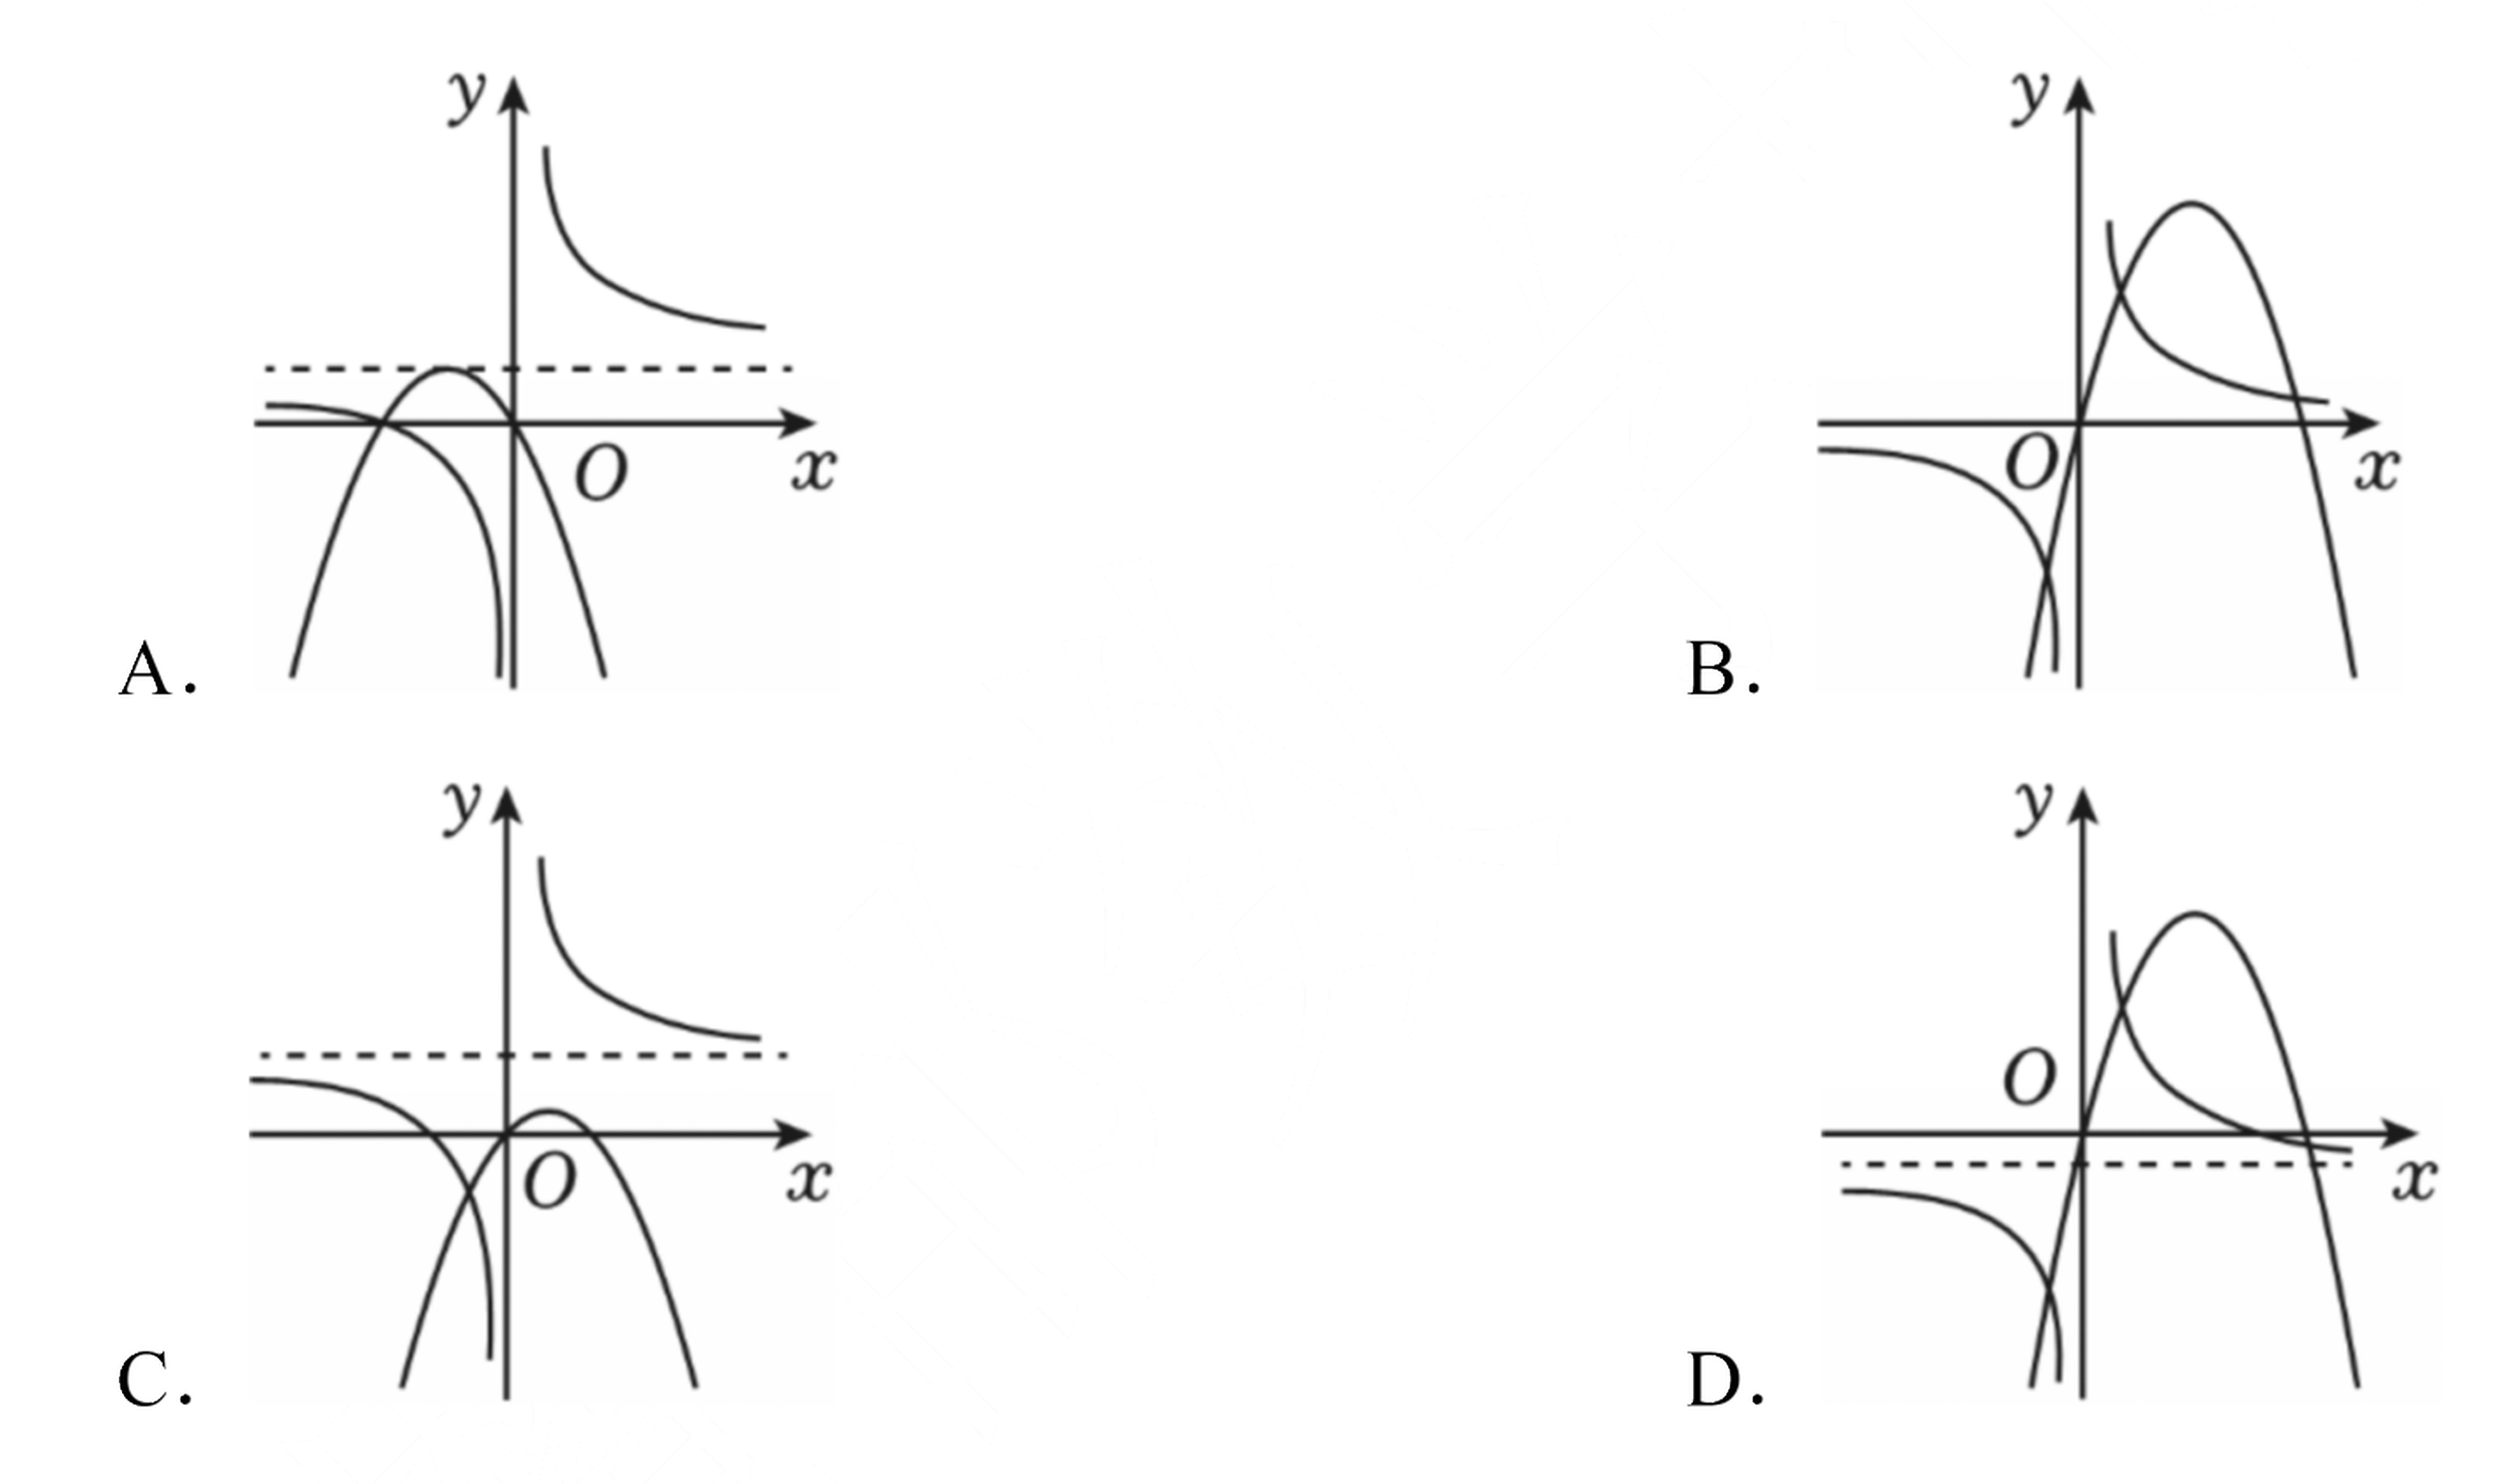
\includegraphics[width=0.80\textwidth]{figures/gao161_q14.png}
\end{center}

\ifanswer
\solbegin
\step{$A$ 选项，由二次函数图象得 $a<0$，$b<0$，由幂函数型函数图象得 $a<0$，$b>0$，}
\step{故 $A$ 选项错误；}
\step{$B$ 选项，由二次函数图象得 $a<0$，$b>0$，由幂函数型函数图象得 $a<0$，$b=0$，}
\step{故 $B$ 选项错误；}
\step{$C$ 选项，由二次函数图象得 $a<0$，$b>0$，由幂函数型函数图象得 $a<0$，$b>0$，}
\step{故 $C$ 选项正确；}
\step{$D$ 选项，由二次函数图象得 $a<0$，$b>0$，由幂函数型函数图象得 $a<0$，$b<0$，}
\step{故 $D$ 选项错误.}
\step{故选 $C$.}
\solend
\fi

% === Q15 === \subseteq／\subset、\varnothing、\mid；"排除 C""排除 B、D"正体字母照录；解析 4 行，故选 $A$
\item 设不等式 $\lvert f(x)\rvert+\lvert g(x)\rvert<a$（常数 $a>0$）的解集是 $M$，设不等式 $\lvert f(x)+g(x)\rvert<a$（常数 $a>0$）的解集是 $N$，则\mbox{（\quad）}

\keepwithprev
A. $M\subseteq N$\qquad B. $N\subseteq M$\qquad C. $M\subset N$\qquad D. $N\subset M$

\ifanswer
\solbegin
\step{$x\in M\Rightarrow\lvert f(x)+g(x)\rvert\leqslant\lvert f(x)\rvert+\lvert g(x)\rvert<a\Rightarrow x\in N$，所以 $M\subseteq N$.}
\step{取 $f(x)=g(x)=0$，则 $M=N$，排除 C.}
\step{取 $f(x)=1$，$g(x)=-1$，$a=1$，则 $M=\varnothing$，$N$ 为全体实数，排除 B、D.}
\step{故选 $A$.}
\solend
\fi

% === Q16 === "人文集"定义证明；cases 无；解析 21 行，故选 $B$
\item 设集合 $I_n=\{1,2,\cdots,n\}$，$n\in\N,n\geqslant1$，集合 $P_n=\left\{\dfrac{m}{\sqrt k}\mid m\in I_n,k\in I_n\right\}$，若 $P_n$ 的子集 $A$ 中任意两个元素之和不是整数的平方，则称 $A$ 为 “人文集”. 那么使 $P_n$ 能分成两个交集为空集的 “人文集” 的并集，且这两个人文集的并集恰为 $P_n$ 时，$n$ 的最大值是\mbox{（\quad）}

\keepwithprev
A. 13\qquad B. 14\qquad C. 15\qquad D. 16

\ifanswer
\solbegin
\step{先证当 $n\geqslant15$ 时，$P_n$ 不能分成两个不相交的人文集的并集.}
\step{假设当 $n\geqslant15$ 时，$P_n$ 可以分成两个不相交的人文集的并集，}
\step{设 $A$ 和 $B$ 为两个不相交的人文集，使 $A\cup B=P_n\supseteq I_n$.}
\step{不妨设 $1\in A$，则由于 $1+3=2^2$，所以 $3\notin A$，即 $3\in B$.}
\step{同理可得，$6\in A$，$10\in B$. 又推出 $15\in A$，}
\step{但 $1+15=4^2$，这与 $A$ 为人文集相矛盾.}
\step{再证 $P_{14}$ 满足要求. 当 $k=1$ 时，$P_{14}=\left\{\dfrac{m}{\sqrt k}\mid m\in I_{14},k\in I_{14}\right\}$，}
\step{可以分成 2 个人文集的并集.}
\step{事实上，只要取 $A_1=\{1,2,4,6,9,11,13\}$，$B_1=\{3,5,7,8,10,12,14\}$，}
\step{则 $A_1$ 和 $B_1$ 都是人文集，且 $A_1\cup B_1=P_{14}$.}
\step{当 $k=4$ 时，集合 $\left\{\dfrac{m}{\sqrt k}\mid m\in I_{14}\right\}$ 中，除整数外，}
\step{剩下的数组成集合 $\left\{\dfrac12,\dfrac32,\dfrac52,\cdots,\dfrac{13}{2}\right\}$，}
\step{可以分为下列 2 个人文集的并：$A_2=\left\{\dfrac12,\dfrac52,\dfrac92,\dfrac{11}{2}\right\}$，$B_2=\left\{\dfrac32,\dfrac72,\dfrac{13}{2}\right\}$.}
\step{当 $k=9$ 时，集合 $\left\{\dfrac{m}{\sqrt k}\mid m\in I_{14}\right\}$ 中，除整数外，}
\step{剩下的数组成集合 $\left\{\dfrac13,\dfrac23,\dfrac43,\dfrac53,\cdots,\dfrac{13}{3},\dfrac{14}{3}\right\}$，}
\step{可以分为下列 2 个人文集的并：$A_3=\left\{\dfrac13,\dfrac43,\dfrac53,\dfrac{10}{3},\dfrac{13}{3}\right\}$，$B_3=\left\{\dfrac23,\dfrac73,\dfrac83,\dfrac{11}{3},\dfrac{14}{3}\right\}$.}
\step{最后，集合 $C=\left\{\dfrac{m}{\sqrt k}\mid m\in I_{14},k\in I_{14},k\ne1,4,9\right\}$ 中的数的分母都是无理数，}
\step{它与 $P_n$ 中的任何其他数之和都不是整数，}
\step{因此，令 $A=A_1\cup A_2\cup A_3\cup C$，$B=B_1\cup B_2\cup B_3$，}
\step{则 $A$ 和 $B$ 是不相交的人文集，且 $A\cup B=P_{14}$.}
\step{综上，$n$ 的最大值为 14，故选 $B$.}
\solend
\fi

\end{enumerate}

\bigsec{三、解答题}

\begin{enumerate}
\setcounter{enumi}{16}

% === Q17 === "图像"照录；\Z；cases 块；解析 9 行，跨 06—07 页
\item (1) 已知函数 $y=x^{\frac{4m-m^2}{2}}$（$m\in\Z$）在区间 $(0,+\infty)$ 上是严格增函数，它的图像关于 $y$ 轴对称，求 $m$ 的值及该函数的解析式；

(2) 若 $(a-2)^{\frac32}<(1+2a)^{\frac32}$，求实数 $a$ 的取值范围.

\ifanswer
\solbegin
\step{(1) 由幂函数在 $(0,+\infty)$ 上严格递增，得 $\dfrac{4m-m^2}{2}>0\Leftrightarrow0<m<4$，}
\step{又 $m\in\Z$，所以 $m\in\{1,2,3\}$.}
\step{当 $m=1$ 或 $m=3$ 时，函数为 $y=x^{\frac32}$，定义域为 $[0,+\infty)$，}
\step{图像不关于 $y$ 轴对称.}
\step{当 $m=2$ 时，函数为 $y=x^2$，满足题意，所以 $m=2$，解析式 $y=x^2$.}
\step{(2) 原不等式有意义，须满足 $\begin{cases}a-2\geqslant0\\1+2a\geqslant0\end{cases}\Leftrightarrow a\geqslant2$，}
\step{函数 $y=x^{\frac32}$ 在 $[0,+\infty)$ 上严格递增，}
\step{因此 $(a-2)^{\frac32}<(1+2a)^{\frac32}\Leftrightarrow a-2<1+2a\Leftrightarrow a>-3$，}
\step{结合 $a\geqslant2$，得 $a\in[2,+\infty)$.}
\solend
\fi

% === Q18 === 题干"$a\geqslant0$"与解析"$a<0$"自相矛盾照录；"$A\cap B=(-2,-1]\cap[2,6)$"误印 ∩ 照录；\subseteq；解析 10 行
\item 已知实数 $a\geqslant0$，集合 $A=\left\{x\mid\dfrac{x+2}{x-6}<0\right\}$，$B=\{x\mid\lvert2x-1\rvert\geqslant3\}$，$C=\{x\mid x^2-3ax+2a^2<0\}$，

(1) 求 $A\cap B$；

(2) 若 $C\subseteq(A\cap B)$，求 $a$ 的取值范围.

\ifanswer
\solbegin
\step{(1) 由 $\dfrac{x+2}{x-6}<0$ 得 $-2<x<6$，即 $A=\{x\mid-2<x<6\}=(-2,6)$，}
\step{由 $\lvert2x-1\rvert\geqslant3$ 得 $2x-1\geqslant3$ 或 $2x-1\leqslant-3$，解得 $x\geqslant2$ 或 $x\leqslant-1$，}
\step{即 $B=(-\infty,-1]\cup[2,+\infty)$，}
\step{所以 $A\cap B=(-2,-1]\cap[2,6)$；}% 原卷把 ∪ 误印成 ∩，照录未改（见 ⑤ 2）
\step{(2) 由 (1) 得 $A\cap B=\{x\mid-2<x\leqslant-1\text{ 或 }2\leqslant x<6\}$，}
\step{因为 $C\subseteq(A\cap B)$，$x^2-3ax+2a^2=(x-a)(x-2a)<0$，}% 题干 $a\geqslant0$ 与解析 $a<0$ 自相矛盾，照录未改（见 ⑤ 1）
\step{当 $a=0$ 时，$C=\varnothing$，符合题意；}
\step{当 $a>0$ 时，$C=(a,2a)$，则 $\begin{cases}a\geqslant2\\2a\leqslant6\\a>0\end{cases}$，解得 $2\leqslant a\leqslant3$，}
\step{当 $a<0$ 时，$C=(2a,a)$，则 $\begin{cases}2a\geqslant-2\\a\leqslant-1\\a<0\end{cases}$，解得 $a=-1$，}
\step{故 $a$ 的范围为 $\{-1,0\}\cup[2,3]$.}
\solend
\fi

% === Q19 === 双碳太阳能应用题；"双碳""自发自用、市电互补"弯引号；解析 8 行，跨 08 页上下
\item 为响应 “双碳” 目标，某电子企业拟安装一套可使用 10 年的太阳能供电设备. 该设备的安装费用 $P(x)$（单位：万元）与太阳能电池板面积 $x(x>0)$（单位：平方米）成正比，比例系数为 $\dfrac12$. 为保障生产用电，安装后采用 “自发自用、市电互补” 模式，在此模式下，企业每年消耗的电费 $Q(x)$（单位：万元）与安装的这种太阳能电池板的面积 $x$ 之间的函数关系是 $Q(x)=\dfrac{180}{x+5}$. 记 $W(x)$（单位：万元）为该企业安装这种太阳能供电设备的费用与 10 年所消耗的电费之和.

(1) 要使该设备的安装费与第 1 年的电费之和不超过 17 万元，求安装太阳能电池板面积 $x$ 的取值范围；

(2) 当 $x$ 为多少平方米时，$W(x)$ 取得最小值？最小值是多少万元？

\ifanswer
\solbegin
\step{(1) $P(x)=\dfrac{x}{2}$，安装费与第 1 年的电费之和不超过 17 万元，即 $\dfrac{x}{2}+\dfrac{180}{x+5}\leqslant17$，}
\step{$x>0$，上式等价于 $x^2-29x+190\leqslant0\Leftrightarrow(x-10)(x-19)\leqslant0$，}
\step{解得 $x\in[10,19]$.}
\step{(2) 安装费用与 10 年电费之和为 $W(x)=P(x)+10Q(x)$，}
\step{$=\dfrac{x}{2}+\dfrac{1800}{x+5}=\dfrac{x+5}{2}+\dfrac{1800}{x+5}-\dfrac52$，}
\step{$x>0$，由基本不等式得 $W(x)\geqslant2\sqrt{\dfrac{x+5}{2}\cdot\dfrac{1800}{x+5}}-\dfrac52=60-\dfrac52=57.5$，}
\step{等号当且仅当 $\dfrac{x+5}{2}=\dfrac{1800}{x+5}$，即 $x=55$ 时成立.}
\step{因此，当电池板面积为 55 平方米时，$W(x)$ 取得最小值 57.5 万元.}
\solend
\fi

% === Q20 === $a*b$ 定义；\min 改正体；cases 块；解析 23 行，跨 08—10 页
\item 设 $a$、$b\in\R$，定义 $a*b=\begin{cases}a,&a<b\\b,&a\geqslant b\end{cases}$.

(1) 若 $x*2>1$，求 $x$ 的取值范围；

(2) 若 $(\lvert x-1\rvert+\lvert x-2\rvert)*3=3$，求 $x$ 的取值范围；

(3) 若 $a$、$b>0$，记 $M=a*\dfrac{b}{a^2+4b^2}$，分别比较 $M$ 与 $a$，以及 $M$ 与 $\dfrac{b}{a^2+4b^2}$ 的大小，并求 $M$ 的最大值.

\ifanswer
\solbegin
\step{(1) 定义 $a*b=\begin{cases}a,&a<b\\b,&a\geqslant b\end{cases}$，由 $x*2>1$，得 $\begin{cases}x<2\\x>1\end{cases}$，或 $\begin{cases}x\geqslant2\\2>1\end{cases}$，}
\step{解得 $x>1$，即 $x$ 的取值范围为 $\{x\mid x>1\}$；}
\step{(2) 当 $x\geqslant2$ 时，$\lvert x-1\rvert+\lvert x-2\rvert=2x-3\geqslant1$，}
\step{当 $1\leqslant2x-3\leqslant3$，即 $2\leqslant x\leqslant3$ 时，}
\step{此时 $(\lvert x-1\rvert+\lvert x-2\rvert)*3=2x-3=3$，解得 $x=3$；}
\step{当 $2x-3>3$，即 $x>3$ 时，}
\step{此时 $(\lvert x-1\rvert+\lvert x-2\rvert)*3=3$ 恒成立，则 $x>3$；}
\step{当 $-2x+3>3$，即 $x<0$ 时，}
\step{此时 $(\lvert x-1\rvert+\lvert x-2\rvert)*3=3$ 恒成立，则 $x<0$.}
\step{当 $1<x<2$ 时，$\lvert x-1\rvert+\lvert x-2\rvert=1$，}
\step{此时 $(\lvert x-1\rvert+\lvert x-2\rvert)*3=1\ne3$，不符合题意；}
\step{当 $x\leqslant1$ 时，$\lvert x-1\rvert+\lvert x-2\rvert=-2x+3\geqslant1$，}
\step{当 $-2x+3\leqslant3$，即 $0\leqslant x\leqslant1$ 时，}
\step{此时 $(\lvert x-1\rvert+\lvert x-2\rvert)*3=-2x+3=3$，解得 $x=0$.}
\step{综上所述，$x$ 的取值范围为 $\{x\mid x\leqslant0\text{ 或 }x\geqslant3\}$；}
\step{(3) 由题意，$M=a*\dfrac{b}{a^2+4b^2}=\min\left\{a,\dfrac{b}{a^2+4b^2}\right\}$，}% 原卷印斜体 min，按全稿惯例改正体 \min（见 ② ⑬）
\step{则 $M\leqslant a$，$M\leqslant\dfrac{b}{a^2+4b^2}$.}
\step{因为 $a$、$b>0$，所以 $\dfrac{b}{a^2+4b^2}\leqslant\dfrac{b}{2\sqrt{a^2\cdot4b^2}}=\dfrac{1}{4a}$，}
\step{当且仅当 $a=2b>0$ 时取等号，}
\step{当 $a\geqslant\dfrac{1}{4a}$，即 $a\geqslant\dfrac12$ 时，$M=a*\dfrac{b}{a^2+4b^2}=\dfrac{b}{a^2+4b^2}\leqslant\dfrac{1}{4a}$，}
\step{则 $a=\dfrac12$，$b=\dfrac14$ 时，$M$ 取得最大值 $\dfrac12$；}
\step{当 $0<a<\dfrac12$ 时，$M=a*\dfrac{b}{a^2+4b^2}=a$，此时 $M<\dfrac12$.}
\step{综上所述，$M$ 的最大值为 $\dfrac12$.}
\solend
\fi

% === Q21 === $A_n$／$B_n$／$S_n$／$T_n$ 新定义；题干第 3 问误标 (2) 照录、解析作 (3)；\prec；解析 25 行，跨 10—11 页
\item 对任意正整数 $n$，记集合 $A_n=\{(a_1,a_2,\cdots,a_n)\mid a_1,a_2,\cdots,a_n$ 均为非负整数，且 $a_1+a_2+\cdots+a_n=n\}$，集合 $B_n=\{(b_1,b_2,\cdots,b_n)\mid b_1,b_2,\cdots,b_n$ 均为非负整数，且 $b_1+b_2+\cdots+b_n=2n\}$. 设 $\alpha=(a_1,a_2,\cdots,a_n)\in A_n$，$\beta=(b_1,b_2,\cdots,b_n)\in B_n$，若对任意 $i\in\{1,2,\cdots,n\}$ 都有 $a_i\leqslant b_i$，则记 $\alpha\prec\beta$.

(1) 写出集合 $A_2$ 和 $B_2$；

(2) 证明：对任意 $\alpha\in A_n$，存在 $\beta\in B_n$，使得 $\alpha\prec\beta$；

(2) 设集合 $S_n=\{(\alpha,\beta)\mid\alpha\in A_n,\beta\in B_n,\alpha\prec\beta\}$，求证：$S_n$ 中的元素个数是完全平方数.% 原卷第 3 问题干误标 (2)（与第 2 问重号），照录未改（见 ⑤ 3）

\ifanswer
\solbegin
\step{(1) $A_2=\{(0,2),(1,1),(2,0)\}$，$B_2=\{(0,4),(1,3),(2,2),(3,1),(4,0)\}$；}
\step{(2) 对任意 $\alpha=(a_1,a_2,\cdots,a_n)\in A_n$，设 $b_i=a_i+1$（$i=1,2,3,\cdots,n$），}
\step{则 $b_1,b_2,\cdots,b_n$ 均为非负整数，且 $a_i\leqslant b_i$（$i=1,2,3,\cdots,n$）.}
\step{令 $\beta=(b_1,b_2,\cdots,b_n)$，则 $b_1+b_2+\cdots+b_n$}
\step{$=(a_1+1)+(a_2+1)+\cdots+(a_n+1)=(a_1+a_2+\cdots+a_n)+n=2n$，}
\step{所以 $\beta\in B_n$，且 $\alpha\prec\beta$.}
\step{(3) 对任意 $\alpha=(a_1,a_2,\cdots,a_n)\in A_n$，$\alpha'=(a_1',a_2',\cdots,a_n')\in A_n$，}
\step{记 $\alpha+\alpha'=(a_1+a_1',a_2+a_2',\cdots,a_n+a_n')$，}
\step{则 $a_1+a_1',a_2+a_2',\cdots,a_n+a_n'$ 均为非负整数，}
\step{且 $(a_1+a_1')+(a_2+a_2')+\cdots+(a_n+a_n')$}
\step{$=(a_1+a_2+\cdots+a_n)+(a_1'+a_2'+\cdots+a_n')=n+n=2n$，}
\step{所以 $\alpha+\alpha'\in B_n$，且 $\alpha\prec\alpha+\alpha'$，$\alpha'\prec\alpha+\alpha'$.}
\step{设集合 $A_n$ 中的元素个数为 $t$，设 $A_n=\{\alpha_1,\alpha_2,\cdots,\alpha_t\}$.}
\step{设集合 $T_n=\{(\alpha_i,\alpha_i+\alpha_j)\mid i=1,2,\cdots,t,j=1,2,\cdots,t\}$.}
\step{对任意 $\alpha_i\in A_n$（$i=1,2,\cdots,t$），都有 $\alpha_i+\alpha_1,\alpha_i+\alpha_2,\cdots,\alpha_i+\alpha_t\in B_n$，}
\step{且 $\alpha_i\prec\alpha_i+\alpha_j$，$j=1,2,\cdots,t$，所以 $T_n\subseteq S_n$.}
\step{若 $(\alpha,\beta)\in S_n$，其中 $\alpha=(a_1,a_2,\cdots,a_n)\in A_n$，$\beta=(b_1,b_2,\cdots,b_n)\in B_n$，}
\step{设 $c_i=b_i-a_i$（$i=1,2,\cdots,n$），因为 $a_i\leqslant b_i$，所以 $c_i=b_i-a_i\geqslant0$，}
\step{记 $\alpha'=(c_1,c_2,\cdots,c_n)$，}
\step{则 $c_1+c_2+\cdots+c_n=(b_1-a_1)+(b_2-a_2)+\cdots+(b_n-a_n)$}
\step{$=(b_1+b_2+\cdots+b_n)-(a_1+a_2+\cdots+a_n)=2n-n=n$，}
\step{所以 $\alpha'\in A_n$，并且有 $\beta=\alpha+\alpha'$，所以 $(\alpha,\beta)\in T_n$，所以 $S_n\subseteq T_n$，}
\step{所以 $S_n=T_n$.}
\step{因为集合 $T_n$ 中的元素个数为 $t^2$，所以 $S_n$ 中的元素个数为 $t^2$，}
\step{是完全平方数.}
\solend
\fi

\end{enumerate}

\end{document}
"
% 紧凑版：xelatex "\def\iscompact{1}% 高一161_松江一中嘉一实验_期中.tex
%   —— 高一上数学"2026-2027 年松江一中嘉一实验高一上期中"（试卷版/答案版/紧凑版）
% 试卷版：xelatex 高一161_松江一中嘉一实验_期中.tex
% 答案版：xelatex "\def\isanswer{1}\input{高一161_松江一中嘉一实验_期中.tex}"
% 紧凑版：xelatex "\def\iscompact{1}\input{高一161_松江一中嘉一实验_期中.tex}"
%
% ① 原始材料：微信公众号"魔都数学加油站"文章，连载"27学年高一161"，原卷卷面标题
% "2026-2027 年松江一中嘉一实验高一上期中"（卷面未印副标题、未印连载号）。
% 正文为 11 张 PNG 页（01/02/03/05/06/07/08/09/11 为 4762×6735，04/10 为
% 2560×3620，同一篇各页分辨率混排，逐页按各自分辨率裁图核对）。
% 体例：讲评版——填空 3—12（10 题）、选择 13—16（4 题）、解答 17—21（5 题），
% 共 19 题，自第 3 题起编（1、2 未印在本篇）；Q13 答案"A"直接印在题干括号内、
% 且无【答案】/【解析】段，本稿按 高一37 第 13 题／高一57 第 13 题成例把括号
% 留空、另提 \ans{$A$}；其余 18 题逐题印【解析】、用 \solbegin…\solend。
% 题目、答案、解析均据原图转录；卷面粉红色水印"魔都数学加油站"及公众号页脚未录入。
% 全卷插图清单（逐页通读 11 页确认）：仅 1 组——Q14 四幅图像选项（04 页 2×2
% 排布，二次函数与幂函数型函数在同一坐标系中的图象，A/B/C/D 四幅小图），
% 合并成一张，三版都出，裁 figures/gao161_q14.png。其余各页逐页确认无其它
% 题目配图、无解析内配图、无表格、无"如图"处（Q16 解析里的"可以分为下列 2 个
% 人文集的并"是纯文字＋集合，不是表格；OCR 里看似表格的行实为大括号与分数）。
%
% 卷首标题：原卷印作"2026-2027 年松江一中嘉一实验高一上期中"，年份区间按全稿惯例排 en dash；
% 原卷卷面未印副标题，本稿按同期中卷知识模块口径补出"集合与常用逻辑用语、不等式、函数"。
%
% ② 与原卷的排版差异／照录项清单：
%   ① 原文从第 3 题起，本稿保留原题号；共 19 题三节，解答题 5 题到 21；
%      三节各自一个 enumerate + \setcounter{enumi}{2}/{12}/{16}（不贯穿），
%      用 \examtitlest[3] 起手；
%   ② 混合体例：Q13 原卷把答案"A"直接印在题干括号内（"（  A  ）"）、且题下
%      无【答案】/【解析】段，按 高一37 第 13 题／高一57 第 13 题成例把括号
%      留空、另提 \ans{$A$}、不补造解析；其余 18 题印【解析】、用
%      \solbegin…\solend；四道选择题中 Q14/Q15/Q16 的答案在解析末句
%      "故选 $C$／$A$／$B$"、Q13 用 \ans{$A$}；括号 \mbox{（\quad）} 留空；
%      答案版【答案】/【解析】标记数 = 19 = 全卷题数（1 个 \ans ＋ 18 个 \solbegin）；
%   ③ 原卷卷面未印副标题，本稿按知识模块口径补出；
%   ④ 原卷填空横线按全稿惯例排 \blankline[4.4em]；选择题选项段前按惯例各加
%      \keepwithprev；Q14 四幅选项图整块用 \needvspace{9cm} 守卫（守卫放
%      \item 之前，见 高一132 Q14／高一154 Q15 成例）；解答题不留作答区、
%      不加 \anspace（原卷为讲评版）；
%   ⑤ 数集归一：Q8"$x\in\R$"、Q11"$m\in\R$"、Q13"$x,y\in\N$"、
%      Q16"$n\in N$"、Q17"$m\in\Z$"、Q20"$a$、$b\in R$"——原卷印正体粗体
%      或斜体 R/N/Z，按全稿惯例归一 \R／\N／\Z；绝对值排 \lvert…\rvert
%      （Q9、Q12、Q15、Q18、Q20），集合描述竖线排 \mid（Q12、Q16、Q18、
%      Q20、Q21），空集 \varnothing（Q15、Q18），补集无用例，不等号按全稿
%      惯例排 \leqslant／\geqslant；
%   ⑥ 子集符号逐处照录不统一：Q12 cases 定义"$C(A)\geqslant C(B)$"、
%      Q15 选项 A/B"$M\subseteq N$""$N\subseteq M$"与解析"$M\subseteq N$"
%      印带下划线 ⊆（照录 \subseteq），Q15 选项 C/D"$M\subset N$""$N\subset M$"
%      印单线 ⊂（照录 \subset），Q18 "$C\subseteq(A\cap B)$"、Q21
%      "$T_n\subseteq S_n$""$S_n\subseteq T_n$"均带下划线照录 \subseteq；
%      本卷无 \not\subset 用例；
%   ⑦ 判别式：Q7 解析"$\Delta=(m-6)(m+2)>0$"、Q8 解析"$\Delta=a^2-4a<0$"、
%      Q12 解析"$\Delta=a^2-8$"共 3 处，逐处放大确认印等腰偏高粗三角
%      （高>宽、右斜边粗），照录 \Delta；本卷无扁等边细线 \triangle 用例；
%   ⑧ 中文弯引号照录：Q7"$m\geqslant6$""有两个不相等的正实数根"及四个
%      条件短语、Q13 反证法命题、Q16"人文集"、Q19"双碳""自发自用、市电互补"；
%      注释里一律 ASCII 引号；数学式内 CJK 用 \text{}（Q18、Q20 解集描述内"或"）；
%   ⑨ "图像／图象"逐处照录不统一：Q4"的图像"、Q17 题干"它的图像关于 $y$ 轴
%      对称"及解析"图像不关于 $y$ 轴对称"印"图像"；Q14 题干"的图象可能为"
%      与解析 A/B/C/D 四行各"由二次函数图象得""由幂函数型函数图象得"
%      共 8 处印"图象"（象，无亻）；
%   ⑩ 文本圈数字逐处照录：Q12 题干①②③④、Q12 解析"故①错误""故②正确"
%      "故③正确""故④错误""故正确的是②③"，均为印刷圈数字（文本模式）；
%   ⑪ 半角逗号在数学组之间是全稿惯例、非笔误，逐处照录（Q5"$a$、$b$"、
%      Q13"$x,y\in\N$"、Q16"$n\in\N,n\geqslant1$"与集合描述内逗号、
%      Q20"$a,b\in\R$"、Q21 各集合描述内逗号）；行末西文句点 ASCII `.`；
%      原卷行中句点（Q16"$10\in B$. 又推出 $15\in A$"、Q16"再证 $P_{14}$
%      满足要求. 当 $k=1$ 时"、Q18"$A\cap B=(-2,-1]\cap[2,6)$；"后的分号）
%      按全稿惯例一律排 ASCII `.`／全角"；"；中文语境行中全角逗号／顿号照录；
%   ⑫ 原卷数学式内联条件（Q14"$y=x^a+b(a\ne0)$"、Q19"$x(x>0)$"、
%      Q11"$\lvert x-m\rvert<n\,(m\in\R,n>0)$"）印半角括号，逐处照录未改
%      全角（同 高一147 口径）；
%      中文语境的括注（Q5"结果用 $a$、$b$ 表示"、Q7"填…"、Q12"填写序号"、
%      Q15"常数 $a>0$"、Q19"单位：万元"）印全角括号，照录；
%   ⑬ 复杂式照录别简化：Q3 $(a^{2-\sqrt3})^{2+\sqrt3}\times\sqrt{a^2}\times
%      b^{\sqrt3}\times b^{1-\sqrt3}$ 与 $a^{(2-\sqrt3)(2+\sqrt3)}\cdot a\cdot
%      b^{\sqrt3+1-\sqrt3}=a\cdot a\cdot b=a^2b$（题干用 \times、解析用 \cdot，
%      逐处照录不统一，见 ⑤）；Q5 $\dfrac{\lg2}{\lg2+\lg3}=\dfrac{a}{a+b}$、
%      Q10 $t-\dfrac3t=2$ 与 $b=a^3$、$ab=a^4=2$、Q11 $\left(2a-\dfrac12
%      -a+\dfrac12,2a-\dfrac12+a-\dfrac12\right)=(a,3a-1)$ 与
%      $\left(\dfrac43,\dfrac53\right]\cup\{2\}$、Q16 各分数集合、Q19
%      $x^2-29x+190\leqslant0$ 与 $W(x)=P(x)+10Q(x)$ 与
%      $2\sqrt{\dfrac{x+5}{2}\cdot\dfrac{1800}{x+5}}-\dfrac52=60-\dfrac52=57.5$、
%      Q20 $M=a*\dfrac{b}{a^2+4b^2}=\min\left\{a,\dfrac{b}{a^2+4b^2}\right\}$
%      与 $\dfrac{b}{2\sqrt{a^2\cdot4b^2}}=\dfrac{1}{4a}$、Q21 各 $A_n$／$B_n$／
%      $T_n$ 定义；\left…\right 不得拆到不同 $…$ 组（Q11 的 \left(…\right)、
%      Q11 的 \left(\dfrac43,\dfrac53\right]、Q16 的 \left\{\dfrac{m}{\sqrt k}
%      \mid…\right\} 与 \left\{\dfrac12,\dfrac32,\dfrac52,\cdots,\dfrac{13}{2}\right\}
%      等、Q20 的 \min\left\{…\right\}）；cases 块整体算一个印刷行
%      （Q12 定义、Q17 (2)、Q18 (2) 两处、Q20 定义与 (1)）；原卷 Q20 解析
%      "$=min\{…\}$"印斜体 min，按 高一122／高一102 成例改正体 \min；
%   ⑭ 一条 \step = 原卷解析的一个印刷行；别并折行、别拆行。跨页续印按题合并
%      （Q6 的 01 页上下题干重复印、Q10 的 01—02 页、Q11 的 02—03 页、
%      Q12 的 03—04 页、Q16 的 05—06 页、Q17 的 06—07 页、Q18 的 07 页
%      上下、Q19 的 08 页上下、Q20 的 08—10 页、Q21 的 10—11 页）；
%      跨半页重叠行（Q10"令 $t=\log_a b>0$…"、Q16"它与 $P_n$ 中的任何
%      其他数之和都不是整数，"、Q18"【解析】(1) 由 $\dfrac{x+2}{x-6}<0$…"、
%      Q19"$x>0$，上式等价于…"、Q20"此时…则 $x<0$."、Q21"若 $(\alpha,\beta)
%      \in S_n$…"与"设 $c_i=b_i-a_i$…"）只算一个印刷行；
%   ⑮ 自定义记号照录：Q12"$C(A)$""$A*B$""$S$"、Q16"$I_n$""$P_n$""人文集"
%      "$A_1$／$B_1$／$A_2$／$B_2$／$A_3$／$B_3$／$C$"、Q20"$a*b$""$M$"、
%      Q21"$A_n$／$B_n$／$S_n$／$T_n$""$\alpha\prec\beta$""$\alpha+\alpha'$"；
%   ⑯ 选项字母体例照录不统一：Q15 解析"排除 C.""排除 B、D."两处原卷印
%      正体（文本模式），Q13 \ans{$A$}、Q14"$A$ 选项"…"故选 $C$"、
%      Q15"故选 $A$"、Q16"故选 $B$"用斜体（数学模式），逐处照录、不统一；
%   ⑰ 红字：全卷逐页扫描无红色加粗小标题（仅粉色水印），故本卷无 \stepm，
%      不引入红色定义；
%
% ③ 行数复核：一条 \step = 原卷解析的一个印刷行，cases 块作一个印刷行计。
%   逐题数（逐页核对定稿）：Q3：1；Q4：1；Q5：1；Q6：3；Q7：4；Q8：4；
%   Q9：2；Q10：2；Q11：7；Q12：8；Q13：0（答案印括号内、提 \ans{}，
%   不计入 \step 账）；Q14：9；Q15：4；Q16：21；Q17：9；Q18：10；Q19：8；
%   Q20：23；Q21：25。
%   合计 142 行（142 条 \step，无 \stepm），与原卷逐题印刷行相等。
%   全卷 19 题：Q13 一处 \ans{} ＋ 其余 18 题设 \solbegin…\solend，
%   答案版【答案】/【解析】标记数 = 19 = 全卷题数。
%
% ④ 页码分布（供回原图复核）：
%   卷首标题＋"一、填空题"＋Q3/Q4/Q5 题干＋解析各 1 行＋Q6 题干首行
%   在 01 页上半；Q6 题干（重复印）＋解析 3 行＋Q7 题干＋解析 4 行在
%   01 页下半；Q8 题干＋解析 4 行＋Q9 题干＋解析 2 行＋Q10 题干＋
%   解析首行在 02 页上半；Q10 解析（重复印）＋末行＋Q11 题干＋解析
%   前 3 行在 02 页下半；Q11 解析后 4 行＋Q12 题干＋cases 定义＋①
%   在 03 页上半；Q12 ②③④ 三命题＋"填写序号"行＋解析前 6 行在
%   03 页下半；Q12 解析后 2 行＋"二、选择题"标题＋Q13 题干＋选项＋
%   Q14 题干＋"（　）"＋A/B 两幅图在 04 页上半；Q14 四幅图（重复印）
%   ＋解析 9 行在 04 页下半；Q15 题干＋选项＋解析 4 行＋Q16 题干＋
%   选项在 05 页上半；Q16 题干（重复印）＋选项＋解析前 10 行在 05 页
%   下半；Q16 解析中 8 行（k=4、k=9 两批＋集合 C＋"它与 $P_n$…"）
%   在 06 页上半；Q16 解析"它与 $P_n$…"（重复印）＋末 3 行＋
%   "三、解答题"标题＋Q17 题干＋两问＋解析前 4 行在 06 页下半；
%   Q17 解析后 5 行＋Q18 题干＋两问＋解析首行在 07 页上半；Q18 解析
%   （重复首行）＋余 9 行在 07 页下半；Q19 题干＋两问＋解析前 2 行在
%   08 页上半；Q19 解析（重复第 2 行）＋余 6 行＋Q20 定义＋(1) 问在
%   08 页下半；Q20 (2)(3) 两问＋解析 (1) 2 行＋(2) 前 7 行在 09 页
%   上半；Q20 解析 (2) 余 4 行＋(3) 前 4 行在 09 页下半；Q20 解析 (3)
%   余 4 行＋Q21 题干＋三问在 10 页上半；Q21 题干（重复印）＋解析
%   (1)(2)(3) 前 8 行在 10 页下半；Q21 解析 (3) 中 10 行在 11 页上半；
%   Q21 解析 (3)（重复 2 行）＋末 7 行"是完全平方数."在 11 页下半。
%   本稿按题连排，不丢行、不并折行；全卷末题为第 21 题，无附加题节。
%
% ⑤ 存疑照录（放大原图确认，照录未改、正文对应处另有 % 注）：
%   1. Q18 题干印"已知实数 $a\geqslant0$"，解析却另设"当 $a<0$ 时"并解出
%      $a=-1$，末行答案"故 $a$ 的范围为 $\{-1,0\}\cup[2,3]$"含负数，
%      与题干 $a\geqslant0$ 自相矛盾——系原卷前后不一，照录未改（放大
%      07 页确认题干确印 $a\geqslant0$）；
%   2. Q18 解析"所以 $A\cap B=(-2,-1]\cap[2,6)$；"原卷把并集误印成
%      交集号 ∩（紧接下一行"$A\cap B=\{x\mid-2<x\leqslant-1$ 或
%      $2\leqslant x<6\}$"用"或"），照录未改（放大 07 页确认印 ∩）；
%   3. Q21 题干第 3 问原卷标号印作"(2)"（与第 2 问重号），而解析里
%      同一问标作"(3)"——原卷笔误，题干与解析逐处照录、不统一；
%   4. Q3 题干四处乘号印"×"（\times）、解析内三处乘号印"·"（\cdot），
%      逐处照录未统一（放大 01 页确认）；
%   5. Q16 解析"先证当 $n\geqslant15$ 时"印 ≥（非 >），与"综上，$n$
%      的最大值为 14"自洽，照录；题干"$n\in N,n\geqslant1$"印斜体
%      $N$、按全稿惯例归一 \N（见 ② ⑤）；
%   6. Q20 解析"$M=a*\dfrac{b}{a^2+4b^2}=min\{…\}$"原卷印斜体 min，
%      按全稿惯例改正体 \min（见 ② ⑬）；末行"$M$ 的最大值为
%      $\dfrac12$"照录；
%   7. Q15 解析"排除 C.""排除 B、D."用正体字母，而"故选 $A$"用斜体
%      字母，原卷体例不一（见 ② ⑯），照录未统一。
%   全卷除此 7 类外未发现其它笔误／自相矛盾处；Q13 只把答案印在括号内、
%   其余 18 题全部印【解析】。
%

\documentclass[a4paper,11pt]{article}
\usepackage{common}

\begin{document}

\examtitlest[3]{2026--2027 年松江一中嘉一实验高一上期中}{集合与常用逻辑用语、不等式、函数}

\bigsec{一、填空题}

\begin{enumerate}
\setcounter{enumi}{2}

% === Q3 === 题干 \times、解析 \cdot 逐处照录；解析 1 行
\item 设 $a>0$，$b>0$，化简 $(a^{2-\sqrt3})^{2+\sqrt3}\times\sqrt{a^2}\times b^{\sqrt3}\times b^{1-\sqrt3}=$\blankline[4.4em].

\ifanswer
\solbegin
\step{因为 $a>0$，所以 $\sqrt{a^2}=a$，原式 $=a^{(2-\sqrt3)(2+\sqrt3)}\cdot a\cdot b^{\sqrt3+1-\sqrt3}=a\cdot a\cdot b=a^2b$.}
\solend
\fi

% === Q4 === "图像"照录；解析 1 行
\item 若幂函数 $y=x^a$ 的图像经过点 $(5,\sqrt5)$，则此幂函数的表达式为 $y=$\blankline[4.4em].

\ifanswer
\solbegin
\step{$5^a=\sqrt5\Rightarrow a=\dfrac12$，所以 $y=\sqrt x$.}
\solend
\fi

% === Q5 === "结果用 $a$、$b$ 表示"全角括号＋顿号照录；解析 1 行
\item 已知 $\lg2=a$，$10^b=3$，则 $\log_6 2=$\blankline[4.4em]（结果用 $a$、$b$ 表示）.

\ifanswer
\solbegin
\step{$\lg3=b$，$\log_6 2=\dfrac{\lg2}{\lg2+\lg3}=\dfrac{a}{a+b}$.}
\solend
\fi

% === Q6 === 对称中心；解析 3 行，题干跨 01 页上下重复印
\item 若函数 $y=\dfrac{mx-1}{x+n}$ 的对称中心是 $(4,-3)$，则 $m+n=$\blankline[4.4em].

\ifanswer
\solbegin
\step{令 $x=-n+t$（$t\ne0$），则 $y-m=-\dfrac{mn+1}{t}$；}
\step{将 $t$ 换成 $-t$，$y-m$ 变为其相反数，因此对称中心为 $(-n,m)$.}
\step{于是 $n=-4$，$m=-3$，得 $m+n=-7$.}
\solend
\fi

% === Q7 === 充要条件；中文弯引号＋圈选条件；\Delta 高瘦；解析 4 行
\item 已知关于 $x$ 的一元二次方程 $x^2-mx+m+3=0$，则 “$m\geqslant6$” 是该方程 “有两个不相等的正实数根” 的\blankline[4.4em]条件（填 “充分不必要”、“必要不充分”、“充要” 或 “既不充分也不必要”）.

\ifanswer
\solbegin
\step{方程有两个不相等的正实数根}
\step{$\Leftrightarrow m>0$、$m+3>0$ 且 $\Delta=(m-6)(m+2)>0\Leftrightarrow m>6$.}
\step{$m>6\Rightarrow m\geqslant6$，但 $m=6$ 时方程有两个相等的正实数根，}
\step{因此为必要不充分条件.}
\solend
\fi

% === Q8 === \R、\Delta；解析 4 行
\item 对于任意的 $x\in\R$，代数式 $\lg(ax^2+ax+1)$ 都有意义，则实数 $a$ 的取值范围是\blankline[4.4em].

\ifanswer
\solbegin
\step{真数须满足 $ax^2+ax+1>0$ 对任意 $x\in\R$ 恒成立.}
\step{$a=0$ 时成立；}
\step{$a\ne0$ 时，恒成立等价于 $a>0$ 且 $\Delta=a^2-4a<0$，解得 $0<a<4$；}
\step{因此 $a\in[0,4)$.}
\solend
\fi

% === Q9 === 绝对值 \lvert…\rvert；解析 2 行
\item 若不等式 $\lvert x+1\rvert-\lvert x-4\rvert<m$ 的解集为非空集合，则实数 $m$ 的取值范围是\blankline[4.4em].

\ifanswer
\solbegin
\step{$\lvert x+1\rvert-\lvert x-4\rvert\geqslant-\lvert(x+1)-(x-4)\rvert=-5$，当 $x=-1$ 时取等号，}
\step{因此原不等式的解集非空 $\Leftrightarrow m>-5$，所求范围为 $(-5,+\infty)$.}
\solend
\fi

% === Q10 === 换底；$\log_2 a\cdot\log_2 b$；解析 2 行，跨 02 页上下
\item 已知 $a>1$，$b>1$，若 $\log_a b-3\log_b a=2$，且 $ab=2$，则 $\log_2 a\cdot\log_2 b=$\blankline[4.4em].

\ifanswer
\solbegin
\step{令 $t=\log_a b>0$，则 $t-\dfrac{3}{t}=2\Leftrightarrow(t-3)(t+1)=0$，得 $t=3$，}
\step{于是 $b=a^3$，$ab=a^4=2$，得 $\log_2 a=\dfrac14$，$\log_2 b=\dfrac34$，所求为 $\dfrac{3}{16}$.}
\solend
\fi

% === Q11 === 邻域定义；\left(…\right) 不拆组；解析 7 行，跨 02—03 页
\item 对于实数 $m$ 和正数 $n$，称满足不等式 $\lvert x-m\rvert<n\,(m\in\R,n>0)$ 的实数 $x$ 的集合叫做 $m$ 的 $n$ 邻域. 已知 $a>\dfrac12$，若 $2a-\dfrac12$ 的 $a-\dfrac12$ 邻域中恰有 2 个整数，则 $a$ 的取值范围是\blankline[4.4em].

\ifanswer
\solbegin
\step{所求邻域为 $\left(2a-\dfrac12-a+\dfrac12,2a-\dfrac12+a-\dfrac12\right)=(a,3a-1)$.}
\step{当 $\dfrac12<a\leqslant1$ 时至多含 1 个整数；}
\step{当 $a>2$ 时，区间长度 $2a-1>3$，至少含 3 个整数.}
\step{当 $1<a<2$ 时，区间必含 2，恰有两个整数等价于 $3<3a-1\leqslant4$，}
\step{即 $\dfrac43<a\leqslant\dfrac53$.}
\step{当 $a=2$ 时，区间为 $(2,5)$，恰含整数 $3,4$；}
\step{所以 $a\in\left(\dfrac43,\dfrac53\right]\cup\{2\}$.}
\solend
\fi

% === Q12 === $C(A)$／$A*B$ 定义题；①②③④ 文本圈数字；\subseteq／\subset、\Delta、\mid、\varnothing；解析 8 行
\item 用 $C(A)$ 表示非空集合 $A$ 中的元素个数. 对于集合 $A$、$B$，定义

$A*B=\begin{cases}C(A)-C(B),&C(A)\geqslant C(B)\\ C(B)-C(A),&C(A)<C(B)\end{cases}$，若 $A=\{0,1\}$，$B=\{x\mid(x^2-ax)(x^2+ax+2)=0\}$，设实数 $a$ 的所有可能取值组成的集合是 $S$，则下列说法正确的是\blankline[4.4em]（填写序号）.

① $C(B)$ 的可能值为 $2,3,4$

② 若 $A*B=2$，则 $a$ 的取值范围为 $(-\infty,-2\sqrt2)\cup(2\sqrt2,+\infty)$

③ 若 $A*B=1$，则 $C(S)=3$

④ 若 $A*B=0$，则 $a$ 的取值范围为 $(-2\sqrt2,2\sqrt2)$

\ifanswer
\solbegin
\step{$x(x-a)=0$ 的根为 $0,a$，而 $x^2+ax+2$ 在这两处的值分别为 $2,2a^2+2$，}
\step{两个因式无公共实根；后者的判别式为 $\Delta=a^2-8$.}
\step{当 $a=0$、$0<\lvert a\rvert<2\sqrt2$、$\lvert a\rvert=2\sqrt2$、$\lvert a\rvert>2\sqrt2$ 时，$C(B)$ 依次为 $1,2,3,4$，}
\step{故①错误.}
\step{$A*B=\lvert2-C(B)\rvert$，所以 $A*B=2\Leftrightarrow\lvert a\rvert>2\sqrt2$，故②正确；}
\step{$A*B=1\Leftrightarrow a\in\{-2\sqrt2,0,2\sqrt2\}$，此时 $C(S)=3$，故③正确；}
\step{$A*B=0\Leftrightarrow0<\lvert a\rvert<2\sqrt2$，即 $a\in(-2\sqrt2,0)\cup(0,2\sqrt2)$，故④错误.}
\step{故正确的是②③.}
\solend
\fi

\end{enumerate}

\needvspace{7cm}
\bigsec{二、选择题}

\begin{enumerate}
\setcounter{enumi}{12}

% === Q13 === 答案"A"原卷印在题干括号内、题下无【答案】/【解析】段；按 高一37／高一57 成例另提 \ans{}
\item 用反证法证明命题 “已知 $x>0$，$y>0$，$x,y\in\N$，如果 $xy$ 可被 7 整除，那么 $x$，$y$ 至少有一个能被 7 整除” 时，假设的内容是\mbox{（\quad）}

\keepwithprev
A. $x$、$y$ 都不能被 7 整除\qquad B. $x$、$y$ 都能被 7 整除

C. $x$、$y$ 只有一个能被 7 整除\qquad D. 只有 $x$ 不能被 7 整除

\ifanswer
\ans{$A$}
\fi

% === Q14 === 四幅图像选项（2×2 合并，三版都出）；守卫放 \item 之前；"图象"照录；解析 9 行，故选 $C$
\needvspace{9cm}
\item 函数 $y=ax^2+bx$ 与函数 $y=x^a+b(a\ne0)$ 在同一平面直角坐标系中的图象可能为\mbox{（\quad）}

\keepwithprev
\begin{center}
% 四幅图象选项取 04 页 2×2 排布合并为一张，去粉色水印、转灰度、4× LANCZOS 放大；三版都出
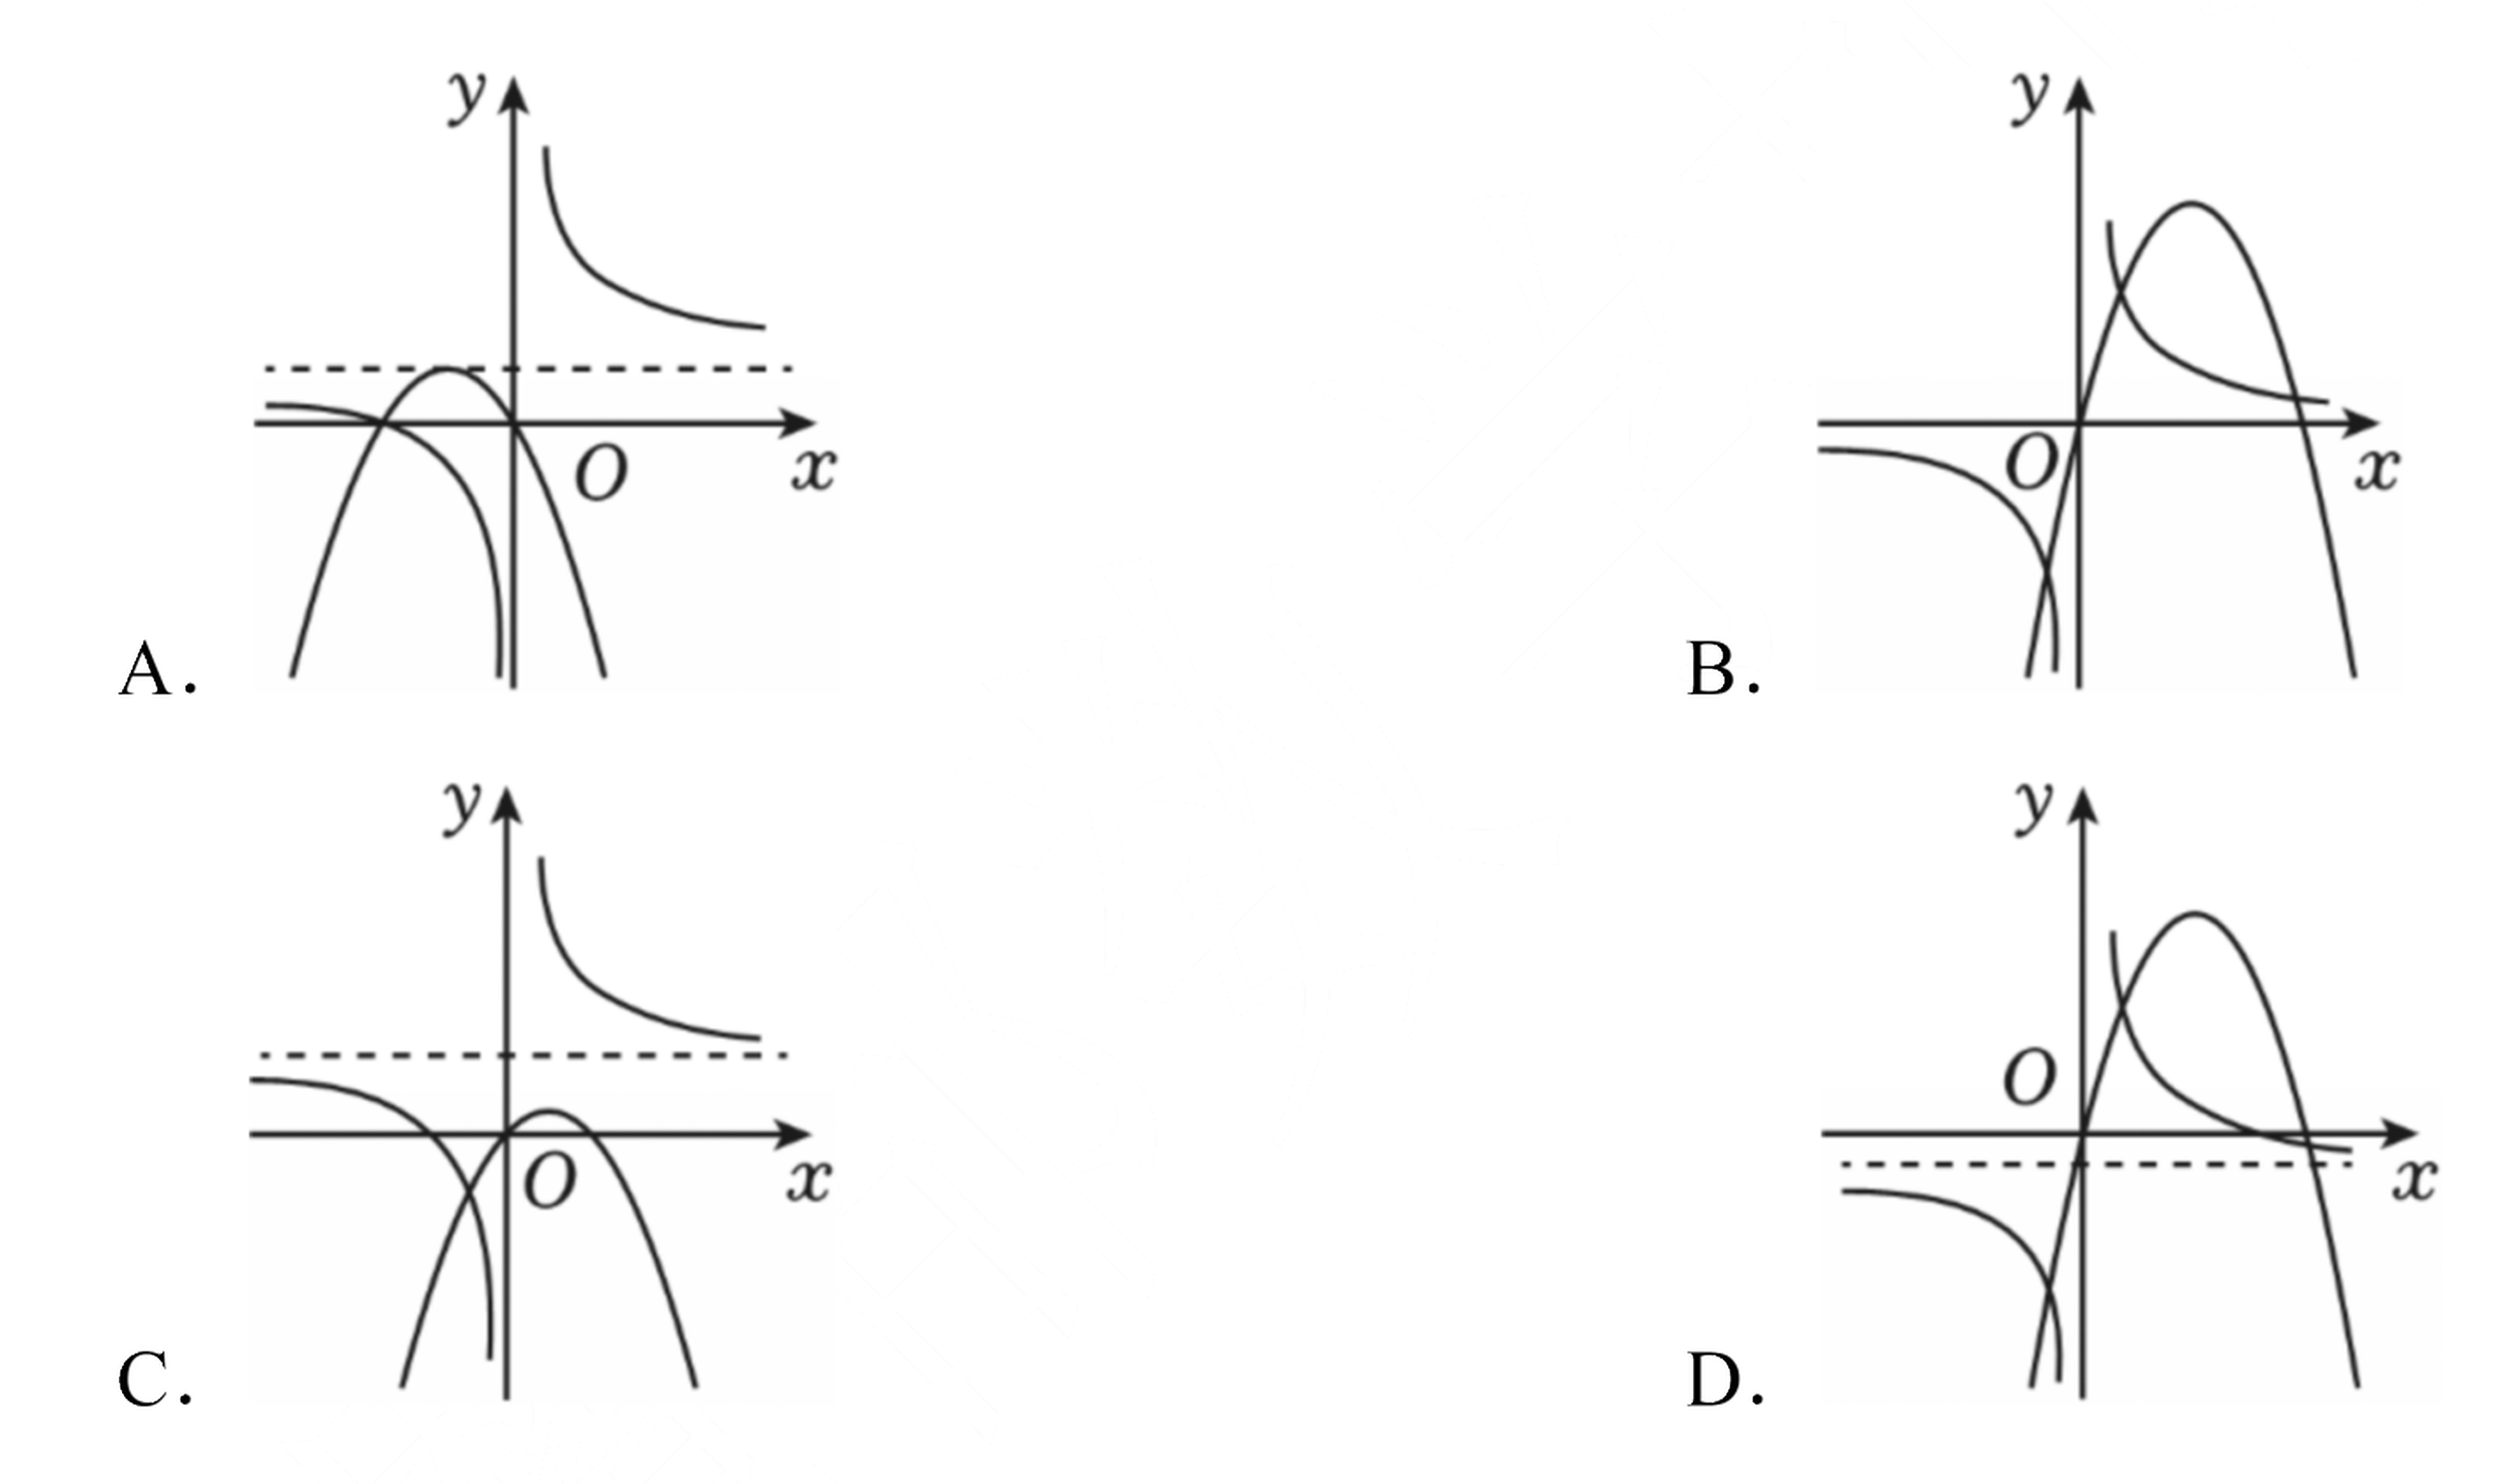
\includegraphics[width=0.80\textwidth]{figures/gao161_q14.png}
\end{center}

\ifanswer
\solbegin
\step{$A$ 选项，由二次函数图象得 $a<0$，$b<0$，由幂函数型函数图象得 $a<0$，$b>0$，}
\step{故 $A$ 选项错误；}
\step{$B$ 选项，由二次函数图象得 $a<0$，$b>0$，由幂函数型函数图象得 $a<0$，$b=0$，}
\step{故 $B$ 选项错误；}
\step{$C$ 选项，由二次函数图象得 $a<0$，$b>0$，由幂函数型函数图象得 $a<0$，$b>0$，}
\step{故 $C$ 选项正确；}
\step{$D$ 选项，由二次函数图象得 $a<0$，$b>0$，由幂函数型函数图象得 $a<0$，$b<0$，}
\step{故 $D$ 选项错误.}
\step{故选 $C$.}
\solend
\fi

% === Q15 === \subseteq／\subset、\varnothing、\mid；"排除 C""排除 B、D"正体字母照录；解析 4 行，故选 $A$
\item 设不等式 $\lvert f(x)\rvert+\lvert g(x)\rvert<a$（常数 $a>0$）的解集是 $M$，设不等式 $\lvert f(x)+g(x)\rvert<a$（常数 $a>0$）的解集是 $N$，则\mbox{（\quad）}

\keepwithprev
A. $M\subseteq N$\qquad B. $N\subseteq M$\qquad C. $M\subset N$\qquad D. $N\subset M$

\ifanswer
\solbegin
\step{$x\in M\Rightarrow\lvert f(x)+g(x)\rvert\leqslant\lvert f(x)\rvert+\lvert g(x)\rvert<a\Rightarrow x\in N$，所以 $M\subseteq N$.}
\step{取 $f(x)=g(x)=0$，则 $M=N$，排除 C.}
\step{取 $f(x)=1$，$g(x)=-1$，$a=1$，则 $M=\varnothing$，$N$ 为全体实数，排除 B、D.}
\step{故选 $A$.}
\solend
\fi

% === Q16 === "人文集"定义证明；cases 无；解析 21 行，故选 $B$
\item 设集合 $I_n=\{1,2,\cdots,n\}$，$n\in\N,n\geqslant1$，集合 $P_n=\left\{\dfrac{m}{\sqrt k}\mid m\in I_n,k\in I_n\right\}$，若 $P_n$ 的子集 $A$ 中任意两个元素之和不是整数的平方，则称 $A$ 为 “人文集”. 那么使 $P_n$ 能分成两个交集为空集的 “人文集” 的并集，且这两个人文集的并集恰为 $P_n$ 时，$n$ 的最大值是\mbox{（\quad）}

\keepwithprev
A. 13\qquad B. 14\qquad C. 15\qquad D. 16

\ifanswer
\solbegin
\step{先证当 $n\geqslant15$ 时，$P_n$ 不能分成两个不相交的人文集的并集.}
\step{假设当 $n\geqslant15$ 时，$P_n$ 可以分成两个不相交的人文集的并集，}
\step{设 $A$ 和 $B$ 为两个不相交的人文集，使 $A\cup B=P_n\supseteq I_n$.}
\step{不妨设 $1\in A$，则由于 $1+3=2^2$，所以 $3\notin A$，即 $3\in B$.}
\step{同理可得，$6\in A$，$10\in B$. 又推出 $15\in A$，}
\step{但 $1+15=4^2$，这与 $A$ 为人文集相矛盾.}
\step{再证 $P_{14}$ 满足要求. 当 $k=1$ 时，$P_{14}=\left\{\dfrac{m}{\sqrt k}\mid m\in I_{14},k\in I_{14}\right\}$，}
\step{可以分成 2 个人文集的并集.}
\step{事实上，只要取 $A_1=\{1,2,4,6,9,11,13\}$，$B_1=\{3,5,7,8,10,12,14\}$，}
\step{则 $A_1$ 和 $B_1$ 都是人文集，且 $A_1\cup B_1=P_{14}$.}
\step{当 $k=4$ 时，集合 $\left\{\dfrac{m}{\sqrt k}\mid m\in I_{14}\right\}$ 中，除整数外，}
\step{剩下的数组成集合 $\left\{\dfrac12,\dfrac32,\dfrac52,\cdots,\dfrac{13}{2}\right\}$，}
\step{可以分为下列 2 个人文集的并：$A_2=\left\{\dfrac12,\dfrac52,\dfrac92,\dfrac{11}{2}\right\}$，$B_2=\left\{\dfrac32,\dfrac72,\dfrac{13}{2}\right\}$.}
\step{当 $k=9$ 时，集合 $\left\{\dfrac{m}{\sqrt k}\mid m\in I_{14}\right\}$ 中，除整数外，}
\step{剩下的数组成集合 $\left\{\dfrac13,\dfrac23,\dfrac43,\dfrac53,\cdots,\dfrac{13}{3},\dfrac{14}{3}\right\}$，}
\step{可以分为下列 2 个人文集的并：$A_3=\left\{\dfrac13,\dfrac43,\dfrac53,\dfrac{10}{3},\dfrac{13}{3}\right\}$，$B_3=\left\{\dfrac23,\dfrac73,\dfrac83,\dfrac{11}{3},\dfrac{14}{3}\right\}$.}
\step{最后，集合 $C=\left\{\dfrac{m}{\sqrt k}\mid m\in I_{14},k\in I_{14},k\ne1,4,9\right\}$ 中的数的分母都是无理数，}
\step{它与 $P_n$ 中的任何其他数之和都不是整数，}
\step{因此，令 $A=A_1\cup A_2\cup A_3\cup C$，$B=B_1\cup B_2\cup B_3$，}
\step{则 $A$ 和 $B$ 是不相交的人文集，且 $A\cup B=P_{14}$.}
\step{综上，$n$ 的最大值为 14，故选 $B$.}
\solend
\fi

\end{enumerate}

\bigsec{三、解答题}

\begin{enumerate}
\setcounter{enumi}{16}

% === Q17 === "图像"照录；\Z；cases 块；解析 9 行，跨 06—07 页
\item (1) 已知函数 $y=x^{\frac{4m-m^2}{2}}$（$m\in\Z$）在区间 $(0,+\infty)$ 上是严格增函数，它的图像关于 $y$ 轴对称，求 $m$ 的值及该函数的解析式；

(2) 若 $(a-2)^{\frac32}<(1+2a)^{\frac32}$，求实数 $a$ 的取值范围.

\ifanswer
\solbegin
\step{(1) 由幂函数在 $(0,+\infty)$ 上严格递增，得 $\dfrac{4m-m^2}{2}>0\Leftrightarrow0<m<4$，}
\step{又 $m\in\Z$，所以 $m\in\{1,2,3\}$.}
\step{当 $m=1$ 或 $m=3$ 时，函数为 $y=x^{\frac32}$，定义域为 $[0,+\infty)$，}
\step{图像不关于 $y$ 轴对称.}
\step{当 $m=2$ 时，函数为 $y=x^2$，满足题意，所以 $m=2$，解析式 $y=x^2$.}
\step{(2) 原不等式有意义，须满足 $\begin{cases}a-2\geqslant0\\1+2a\geqslant0\end{cases}\Leftrightarrow a\geqslant2$，}
\step{函数 $y=x^{\frac32}$ 在 $[0,+\infty)$ 上严格递增，}
\step{因此 $(a-2)^{\frac32}<(1+2a)^{\frac32}\Leftrightarrow a-2<1+2a\Leftrightarrow a>-3$，}
\step{结合 $a\geqslant2$，得 $a\in[2,+\infty)$.}
\solend
\fi

% === Q18 === 题干"$a\geqslant0$"与解析"$a<0$"自相矛盾照录；"$A\cap B=(-2,-1]\cap[2,6)$"误印 ∩ 照录；\subseteq；解析 10 行
\item 已知实数 $a\geqslant0$，集合 $A=\left\{x\mid\dfrac{x+2}{x-6}<0\right\}$，$B=\{x\mid\lvert2x-1\rvert\geqslant3\}$，$C=\{x\mid x^2-3ax+2a^2<0\}$，

(1) 求 $A\cap B$；

(2) 若 $C\subseteq(A\cap B)$，求 $a$ 的取值范围.

\ifanswer
\solbegin
\step{(1) 由 $\dfrac{x+2}{x-6}<0$ 得 $-2<x<6$，即 $A=\{x\mid-2<x<6\}=(-2,6)$，}
\step{由 $\lvert2x-1\rvert\geqslant3$ 得 $2x-1\geqslant3$ 或 $2x-1\leqslant-3$，解得 $x\geqslant2$ 或 $x\leqslant-1$，}
\step{即 $B=(-\infty,-1]\cup[2,+\infty)$，}
\step{所以 $A\cap B=(-2,-1]\cap[2,6)$；}% 原卷把 ∪ 误印成 ∩，照录未改（见 ⑤ 2）
\step{(2) 由 (1) 得 $A\cap B=\{x\mid-2<x\leqslant-1\text{ 或 }2\leqslant x<6\}$，}
\step{因为 $C\subseteq(A\cap B)$，$x^2-3ax+2a^2=(x-a)(x-2a)<0$，}% 题干 $a\geqslant0$ 与解析 $a<0$ 自相矛盾，照录未改（见 ⑤ 1）
\step{当 $a=0$ 时，$C=\varnothing$，符合题意；}
\step{当 $a>0$ 时，$C=(a,2a)$，则 $\begin{cases}a\geqslant2\\2a\leqslant6\\a>0\end{cases}$，解得 $2\leqslant a\leqslant3$，}
\step{当 $a<0$ 时，$C=(2a,a)$，则 $\begin{cases}2a\geqslant-2\\a\leqslant-1\\a<0\end{cases}$，解得 $a=-1$，}
\step{故 $a$ 的范围为 $\{-1,0\}\cup[2,3]$.}
\solend
\fi

% === Q19 === 双碳太阳能应用题；"双碳""自发自用、市电互补"弯引号；解析 8 行，跨 08 页上下
\item 为响应 “双碳” 目标，某电子企业拟安装一套可使用 10 年的太阳能供电设备. 该设备的安装费用 $P(x)$（单位：万元）与太阳能电池板面积 $x(x>0)$（单位：平方米）成正比，比例系数为 $\dfrac12$. 为保障生产用电，安装后采用 “自发自用、市电互补” 模式，在此模式下，企业每年消耗的电费 $Q(x)$（单位：万元）与安装的这种太阳能电池板的面积 $x$ 之间的函数关系是 $Q(x)=\dfrac{180}{x+5}$. 记 $W(x)$（单位：万元）为该企业安装这种太阳能供电设备的费用与 10 年所消耗的电费之和.

(1) 要使该设备的安装费与第 1 年的电费之和不超过 17 万元，求安装太阳能电池板面积 $x$ 的取值范围；

(2) 当 $x$ 为多少平方米时，$W(x)$ 取得最小值？最小值是多少万元？

\ifanswer
\solbegin
\step{(1) $P(x)=\dfrac{x}{2}$，安装费与第 1 年的电费之和不超过 17 万元，即 $\dfrac{x}{2}+\dfrac{180}{x+5}\leqslant17$，}
\step{$x>0$，上式等价于 $x^2-29x+190\leqslant0\Leftrightarrow(x-10)(x-19)\leqslant0$，}
\step{解得 $x\in[10,19]$.}
\step{(2) 安装费用与 10 年电费之和为 $W(x)=P(x)+10Q(x)$，}
\step{$=\dfrac{x}{2}+\dfrac{1800}{x+5}=\dfrac{x+5}{2}+\dfrac{1800}{x+5}-\dfrac52$，}
\step{$x>0$，由基本不等式得 $W(x)\geqslant2\sqrt{\dfrac{x+5}{2}\cdot\dfrac{1800}{x+5}}-\dfrac52=60-\dfrac52=57.5$，}
\step{等号当且仅当 $\dfrac{x+5}{2}=\dfrac{1800}{x+5}$，即 $x=55$ 时成立.}
\step{因此，当电池板面积为 55 平方米时，$W(x)$ 取得最小值 57.5 万元.}
\solend
\fi

% === Q20 === $a*b$ 定义；\min 改正体；cases 块；解析 23 行，跨 08—10 页
\item 设 $a$、$b\in\R$，定义 $a*b=\begin{cases}a,&a<b\\b,&a\geqslant b\end{cases}$.

(1) 若 $x*2>1$，求 $x$ 的取值范围；

(2) 若 $(\lvert x-1\rvert+\lvert x-2\rvert)*3=3$，求 $x$ 的取值范围；

(3) 若 $a$、$b>0$，记 $M=a*\dfrac{b}{a^2+4b^2}$，分别比较 $M$ 与 $a$，以及 $M$ 与 $\dfrac{b}{a^2+4b^2}$ 的大小，并求 $M$ 的最大值.

\ifanswer
\solbegin
\step{(1) 定义 $a*b=\begin{cases}a,&a<b\\b,&a\geqslant b\end{cases}$，由 $x*2>1$，得 $\begin{cases}x<2\\x>1\end{cases}$，或 $\begin{cases}x\geqslant2\\2>1\end{cases}$，}
\step{解得 $x>1$，即 $x$ 的取值范围为 $\{x\mid x>1\}$；}
\step{(2) 当 $x\geqslant2$ 时，$\lvert x-1\rvert+\lvert x-2\rvert=2x-3\geqslant1$，}
\step{当 $1\leqslant2x-3\leqslant3$，即 $2\leqslant x\leqslant3$ 时，}
\step{此时 $(\lvert x-1\rvert+\lvert x-2\rvert)*3=2x-3=3$，解得 $x=3$；}
\step{当 $2x-3>3$，即 $x>3$ 时，}
\step{此时 $(\lvert x-1\rvert+\lvert x-2\rvert)*3=3$ 恒成立，则 $x>3$；}
\step{当 $-2x+3>3$，即 $x<0$ 时，}
\step{此时 $(\lvert x-1\rvert+\lvert x-2\rvert)*3=3$ 恒成立，则 $x<0$.}
\step{当 $1<x<2$ 时，$\lvert x-1\rvert+\lvert x-2\rvert=1$，}
\step{此时 $(\lvert x-1\rvert+\lvert x-2\rvert)*3=1\ne3$，不符合题意；}
\step{当 $x\leqslant1$ 时，$\lvert x-1\rvert+\lvert x-2\rvert=-2x+3\geqslant1$，}
\step{当 $-2x+3\leqslant3$，即 $0\leqslant x\leqslant1$ 时，}
\step{此时 $(\lvert x-1\rvert+\lvert x-2\rvert)*3=-2x+3=3$，解得 $x=0$.}
\step{综上所述，$x$ 的取值范围为 $\{x\mid x\leqslant0\text{ 或 }x\geqslant3\}$；}
\step{(3) 由题意，$M=a*\dfrac{b}{a^2+4b^2}=\min\left\{a,\dfrac{b}{a^2+4b^2}\right\}$，}% 原卷印斜体 min，按全稿惯例改正体 \min（见 ② ⑬）
\step{则 $M\leqslant a$，$M\leqslant\dfrac{b}{a^2+4b^2}$.}
\step{因为 $a$、$b>0$，所以 $\dfrac{b}{a^2+4b^2}\leqslant\dfrac{b}{2\sqrt{a^2\cdot4b^2}}=\dfrac{1}{4a}$，}
\step{当且仅当 $a=2b>0$ 时取等号，}
\step{当 $a\geqslant\dfrac{1}{4a}$，即 $a\geqslant\dfrac12$ 时，$M=a*\dfrac{b}{a^2+4b^2}=\dfrac{b}{a^2+4b^2}\leqslant\dfrac{1}{4a}$，}
\step{则 $a=\dfrac12$，$b=\dfrac14$ 时，$M$ 取得最大值 $\dfrac12$；}
\step{当 $0<a<\dfrac12$ 时，$M=a*\dfrac{b}{a^2+4b^2}=a$，此时 $M<\dfrac12$.}
\step{综上所述，$M$ 的最大值为 $\dfrac12$.}
\solend
\fi

% === Q21 === $A_n$／$B_n$／$S_n$／$T_n$ 新定义；题干第 3 问误标 (2) 照录、解析作 (3)；\prec；解析 25 行，跨 10—11 页
\item 对任意正整数 $n$，记集合 $A_n=\{(a_1,a_2,\cdots,a_n)\mid a_1,a_2,\cdots,a_n$ 均为非负整数，且 $a_1+a_2+\cdots+a_n=n\}$，集合 $B_n=\{(b_1,b_2,\cdots,b_n)\mid b_1,b_2,\cdots,b_n$ 均为非负整数，且 $b_1+b_2+\cdots+b_n=2n\}$. 设 $\alpha=(a_1,a_2,\cdots,a_n)\in A_n$，$\beta=(b_1,b_2,\cdots,b_n)\in B_n$，若对任意 $i\in\{1,2,\cdots,n\}$ 都有 $a_i\leqslant b_i$，则记 $\alpha\prec\beta$.

(1) 写出集合 $A_2$ 和 $B_2$；

(2) 证明：对任意 $\alpha\in A_n$，存在 $\beta\in B_n$，使得 $\alpha\prec\beta$；

(2) 设集合 $S_n=\{(\alpha,\beta)\mid\alpha\in A_n,\beta\in B_n,\alpha\prec\beta\}$，求证：$S_n$ 中的元素个数是完全平方数.% 原卷第 3 问题干误标 (2)（与第 2 问重号），照录未改（见 ⑤ 3）

\ifanswer
\solbegin
\step{(1) $A_2=\{(0,2),(1,1),(2,0)\}$，$B_2=\{(0,4),(1,3),(2,2),(3,1),(4,0)\}$；}
\step{(2) 对任意 $\alpha=(a_1,a_2,\cdots,a_n)\in A_n$，设 $b_i=a_i+1$（$i=1,2,3,\cdots,n$），}
\step{则 $b_1,b_2,\cdots,b_n$ 均为非负整数，且 $a_i\leqslant b_i$（$i=1,2,3,\cdots,n$）.}
\step{令 $\beta=(b_1,b_2,\cdots,b_n)$，则 $b_1+b_2+\cdots+b_n$}
\step{$=(a_1+1)+(a_2+1)+\cdots+(a_n+1)=(a_1+a_2+\cdots+a_n)+n=2n$，}
\step{所以 $\beta\in B_n$，且 $\alpha\prec\beta$.}
\step{(3) 对任意 $\alpha=(a_1,a_2,\cdots,a_n)\in A_n$，$\alpha'=(a_1',a_2',\cdots,a_n')\in A_n$，}
\step{记 $\alpha+\alpha'=(a_1+a_1',a_2+a_2',\cdots,a_n+a_n')$，}
\step{则 $a_1+a_1',a_2+a_2',\cdots,a_n+a_n'$ 均为非负整数，}
\step{且 $(a_1+a_1')+(a_2+a_2')+\cdots+(a_n+a_n')$}
\step{$=(a_1+a_2+\cdots+a_n)+(a_1'+a_2'+\cdots+a_n')=n+n=2n$，}
\step{所以 $\alpha+\alpha'\in B_n$，且 $\alpha\prec\alpha+\alpha'$，$\alpha'\prec\alpha+\alpha'$.}
\step{设集合 $A_n$ 中的元素个数为 $t$，设 $A_n=\{\alpha_1,\alpha_2,\cdots,\alpha_t\}$.}
\step{设集合 $T_n=\{(\alpha_i,\alpha_i+\alpha_j)\mid i=1,2,\cdots,t,j=1,2,\cdots,t\}$.}
\step{对任意 $\alpha_i\in A_n$（$i=1,2,\cdots,t$），都有 $\alpha_i+\alpha_1,\alpha_i+\alpha_2,\cdots,\alpha_i+\alpha_t\in B_n$，}
\step{且 $\alpha_i\prec\alpha_i+\alpha_j$，$j=1,2,\cdots,t$，所以 $T_n\subseteq S_n$.}
\step{若 $(\alpha,\beta)\in S_n$，其中 $\alpha=(a_1,a_2,\cdots,a_n)\in A_n$，$\beta=(b_1,b_2,\cdots,b_n)\in B_n$，}
\step{设 $c_i=b_i-a_i$（$i=1,2,\cdots,n$），因为 $a_i\leqslant b_i$，所以 $c_i=b_i-a_i\geqslant0$，}
\step{记 $\alpha'=(c_1,c_2,\cdots,c_n)$，}
\step{则 $c_1+c_2+\cdots+c_n=(b_1-a_1)+(b_2-a_2)+\cdots+(b_n-a_n)$}
\step{$=(b_1+b_2+\cdots+b_n)-(a_1+a_2+\cdots+a_n)=2n-n=n$，}
\step{所以 $\alpha'\in A_n$，并且有 $\beta=\alpha+\alpha'$，所以 $(\alpha,\beta)\in T_n$，所以 $S_n\subseteq T_n$，}
\step{所以 $S_n=T_n$.}
\step{因为集合 $T_n$ 中的元素个数为 $t^2$，所以 $S_n$ 中的元素个数为 $t^2$，}
\step{是完全平方数.}
\solend
\fi

\end{enumerate}

\end{document}
"
%
% ① 原始材料：微信公众号"魔都数学加油站"文章，连载"27学年高一161"，原卷卷面标题
% "2026-2027 年松江一中嘉一实验高一上期中"（卷面未印副标题、未印连载号）。
% 正文为 11 张 PNG 页（01/02/03/05/06/07/08/09/11 为 4762×6735，04/10 为
% 2560×3620，同一篇各页分辨率混排，逐页按各自分辨率裁图核对）。
% 体例：讲评版——填空 3—12（10 题）、选择 13—16（4 题）、解答 17—21（5 题），
% 共 19 题，自第 3 题起编（1、2 未印在本篇）；Q13 答案"A"直接印在题干括号内、
% 且无【答案】/【解析】段，本稿按 高一37 第 13 题／高一57 第 13 题成例把括号
% 留空、另提 \ans{$A$}；其余 18 题逐题印【解析】、用 \solbegin…\solend。
% 题目、答案、解析均据原图转录；卷面粉红色水印"魔都数学加油站"及公众号页脚未录入。
% 全卷插图清单（逐页通读 11 页确认）：仅 1 组——Q14 四幅图像选项（04 页 2×2
% 排布，二次函数与幂函数型函数在同一坐标系中的图象，A/B/C/D 四幅小图），
% 合并成一张，三版都出，裁 figures/gao161_q14.png。其余各页逐页确认无其它
% 题目配图、无解析内配图、无表格、无"如图"处（Q16 解析里的"可以分为下列 2 个
% 人文集的并"是纯文字＋集合，不是表格；OCR 里看似表格的行实为大括号与分数）。
%
% 卷首标题：原卷印作"2026-2027 年松江一中嘉一实验高一上期中"，年份区间按全稿惯例排 en dash；
% 原卷卷面未印副标题，本稿按同期中卷知识模块口径补出"集合与常用逻辑用语、不等式、函数"。
%
% ② 与原卷的排版差异／照录项清单：
%   ① 原文从第 3 题起，本稿保留原题号；共 19 题三节，解答题 5 题到 21；
%      三节各自一个 enumerate + \setcounter{enumi}{2}/{12}/{16}（不贯穿），
%      用 \examtitlest[3] 起手；
%   ② 混合体例：Q13 原卷把答案"A"直接印在题干括号内（"（  A  ）"）、且题下
%      无【答案】/【解析】段，按 高一37 第 13 题／高一57 第 13 题成例把括号
%      留空、另提 \ans{$A$}、不补造解析；其余 18 题印【解析】、用
%      \solbegin…\solend；四道选择题中 Q14/Q15/Q16 的答案在解析末句
%      "故选 $C$／$A$／$B$"、Q13 用 \ans{$A$}；括号 \mbox{（\quad）} 留空；
%      答案版【答案】/【解析】标记数 = 19 = 全卷题数（1 个 \ans ＋ 18 个 \solbegin）；
%   ③ 原卷卷面未印副标题，本稿按知识模块口径补出；
%   ④ 原卷填空横线按全稿惯例排 \blankline[4.4em]；选择题选项段前按惯例各加
%      \keepwithprev；Q14 四幅选项图整块用 \needvspace{9cm} 守卫（守卫放
%      \item 之前，见 高一132 Q14／高一154 Q15 成例）；解答题不留作答区、
%      不加 \anspace（原卷为讲评版）；
%   ⑤ 数集归一：Q8"$x\in\R$"、Q11"$m\in\R$"、Q13"$x,y\in\N$"、
%      Q16"$n\in N$"、Q17"$m\in\Z$"、Q20"$a$、$b\in R$"——原卷印正体粗体
%      或斜体 R/N/Z，按全稿惯例归一 \R／\N／\Z；绝对值排 \lvert…\rvert
%      （Q9、Q12、Q15、Q18、Q20），集合描述竖线排 \mid（Q12、Q16、Q18、
%      Q20、Q21），空集 \varnothing（Q15、Q18），补集无用例，不等号按全稿
%      惯例排 \leqslant／\geqslant；
%   ⑥ 子集符号逐处照录不统一：Q12 cases 定义"$C(A)\geqslant C(B)$"、
%      Q15 选项 A/B"$M\subseteq N$""$N\subseteq M$"与解析"$M\subseteq N$"
%      印带下划线 ⊆（照录 \subseteq），Q15 选项 C/D"$M\subset N$""$N\subset M$"
%      印单线 ⊂（照录 \subset），Q18 "$C\subseteq(A\cap B)$"、Q21
%      "$T_n\subseteq S_n$""$S_n\subseteq T_n$"均带下划线照录 \subseteq；
%      本卷无 \not\subset 用例；
%   ⑦ 判别式：Q7 解析"$\Delta=(m-6)(m+2)>0$"、Q8 解析"$\Delta=a^2-4a<0$"、
%      Q12 解析"$\Delta=a^2-8$"共 3 处，逐处放大确认印等腰偏高粗三角
%      （高>宽、右斜边粗），照录 \Delta；本卷无扁等边细线 \triangle 用例；
%   ⑧ 中文弯引号照录：Q7"$m\geqslant6$""有两个不相等的正实数根"及四个
%      条件短语、Q13 反证法命题、Q16"人文集"、Q19"双碳""自发自用、市电互补"；
%      注释里一律 ASCII 引号；数学式内 CJK 用 \text{}（Q18、Q20 解集描述内"或"）；
%   ⑨ "图像／图象"逐处照录不统一：Q4"的图像"、Q17 题干"它的图像关于 $y$ 轴
%      对称"及解析"图像不关于 $y$ 轴对称"印"图像"；Q14 题干"的图象可能为"
%      与解析 A/B/C/D 四行各"由二次函数图象得""由幂函数型函数图象得"
%      共 8 处印"图象"（象，无亻）；
%   ⑩ 文本圈数字逐处照录：Q12 题干①②③④、Q12 解析"故①错误""故②正确"
%      "故③正确""故④错误""故正确的是②③"，均为印刷圈数字（文本模式）；
%   ⑪ 半角逗号在数学组之间是全稿惯例、非笔误，逐处照录（Q5"$a$、$b$"、
%      Q13"$x,y\in\N$"、Q16"$n\in\N,n\geqslant1$"与集合描述内逗号、
%      Q20"$a,b\in\R$"、Q21 各集合描述内逗号）；行末西文句点 ASCII `.`；
%      原卷行中句点（Q16"$10\in B$. 又推出 $15\in A$"、Q16"再证 $P_{14}$
%      满足要求. 当 $k=1$ 时"、Q18"$A\cap B=(-2,-1]\cap[2,6)$；"后的分号）
%      按全稿惯例一律排 ASCII `.`／全角"；"；中文语境行中全角逗号／顿号照录；
%   ⑫ 原卷数学式内联条件（Q14"$y=x^a+b(a\ne0)$"、Q19"$x(x>0)$"、
%      Q11"$\lvert x-m\rvert<n\,(m\in\R,n>0)$"）印半角括号，逐处照录未改
%      全角（同 高一147 口径）；
%      中文语境的括注（Q5"结果用 $a$、$b$ 表示"、Q7"填…"、Q12"填写序号"、
%      Q15"常数 $a>0$"、Q19"单位：万元"）印全角括号，照录；
%   ⑬ 复杂式照录别简化：Q3 $(a^{2-\sqrt3})^{2+\sqrt3}\times\sqrt{a^2}\times
%      b^{\sqrt3}\times b^{1-\sqrt3}$ 与 $a^{(2-\sqrt3)(2+\sqrt3)}\cdot a\cdot
%      b^{\sqrt3+1-\sqrt3}=a\cdot a\cdot b=a^2b$（题干用 \times、解析用 \cdot，
%      逐处照录不统一，见 ⑤）；Q5 $\dfrac{\lg2}{\lg2+\lg3}=\dfrac{a}{a+b}$、
%      Q10 $t-\dfrac3t=2$ 与 $b=a^3$、$ab=a^4=2$、Q11 $\left(2a-\dfrac12
%      -a+\dfrac12,2a-\dfrac12+a-\dfrac12\right)=(a,3a-1)$ 与
%      $\left(\dfrac43,\dfrac53\right]\cup\{2\}$、Q16 各分数集合、Q19
%      $x^2-29x+190\leqslant0$ 与 $W(x)=P(x)+10Q(x)$ 与
%      $2\sqrt{\dfrac{x+5}{2}\cdot\dfrac{1800}{x+5}}-\dfrac52=60-\dfrac52=57.5$、
%      Q20 $M=a*\dfrac{b}{a^2+4b^2}=\min\left\{a,\dfrac{b}{a^2+4b^2}\right\}$
%      与 $\dfrac{b}{2\sqrt{a^2\cdot4b^2}}=\dfrac{1}{4a}$、Q21 各 $A_n$／$B_n$／
%      $T_n$ 定义；\left…\right 不得拆到不同 $…$ 组（Q11 的 \left(…\right)、
%      Q11 的 \left(\dfrac43,\dfrac53\right]、Q16 的 \left\{\dfrac{m}{\sqrt k}
%      \mid…\right\} 与 \left\{\dfrac12,\dfrac32,\dfrac52,\cdots,\dfrac{13}{2}\right\}
%      等、Q20 的 \min\left\{…\right\}）；cases 块整体算一个印刷行
%      （Q12 定义、Q17 (2)、Q18 (2) 两处、Q20 定义与 (1)）；原卷 Q20 解析
%      "$=min\{…\}$"印斜体 min，按 高一122／高一102 成例改正体 \min；
%   ⑭ 一条 \step = 原卷解析的一个印刷行；别并折行、别拆行。跨页续印按题合并
%      （Q6 的 01 页上下题干重复印、Q10 的 01—02 页、Q11 的 02—03 页、
%      Q12 的 03—04 页、Q16 的 05—06 页、Q17 的 06—07 页、Q18 的 07 页
%      上下、Q19 的 08 页上下、Q20 的 08—10 页、Q21 的 10—11 页）；
%      跨半页重叠行（Q10"令 $t=\log_a b>0$…"、Q16"它与 $P_n$ 中的任何
%      其他数之和都不是整数，"、Q18"【解析】(1) 由 $\dfrac{x+2}{x-6}<0$…"、
%      Q19"$x>0$，上式等价于…"、Q20"此时…则 $x<0$."、Q21"若 $(\alpha,\beta)
%      \in S_n$…"与"设 $c_i=b_i-a_i$…"）只算一个印刷行；
%   ⑮ 自定义记号照录：Q12"$C(A)$""$A*B$""$S$"、Q16"$I_n$""$P_n$""人文集"
%      "$A_1$／$B_1$／$A_2$／$B_2$／$A_3$／$B_3$／$C$"、Q20"$a*b$""$M$"、
%      Q21"$A_n$／$B_n$／$S_n$／$T_n$""$\alpha\prec\beta$""$\alpha+\alpha'$"；
%   ⑯ 选项字母体例照录不统一：Q15 解析"排除 C.""排除 B、D."两处原卷印
%      正体（文本模式），Q13 \ans{$A$}、Q14"$A$ 选项"…"故选 $C$"、
%      Q15"故选 $A$"、Q16"故选 $B$"用斜体（数学模式），逐处照录、不统一；
%   ⑰ 红字：全卷逐页扫描无红色加粗小标题（仅粉色水印），故本卷无 \stepm，
%      不引入红色定义；
%
% ③ 行数复核：一条 \step = 原卷解析的一个印刷行，cases 块作一个印刷行计。
%   逐题数（逐页核对定稿）：Q3：1；Q4：1；Q5：1；Q6：3；Q7：4；Q8：4；
%   Q9：2；Q10：2；Q11：7；Q12：8；Q13：0（答案印括号内、提 \ans{}，
%   不计入 \step 账）；Q14：9；Q15：4；Q16：21；Q17：9；Q18：10；Q19：8；
%   Q20：23；Q21：25。
%   合计 142 行（142 条 \step，无 \stepm），与原卷逐题印刷行相等。
%   全卷 19 题：Q13 一处 \ans{} ＋ 其余 18 题设 \solbegin…\solend，
%   答案版【答案】/【解析】标记数 = 19 = 全卷题数。
%
% ④ 页码分布（供回原图复核）：
%   卷首标题＋"一、填空题"＋Q3/Q4/Q5 题干＋解析各 1 行＋Q6 题干首行
%   在 01 页上半；Q6 题干（重复印）＋解析 3 行＋Q7 题干＋解析 4 行在
%   01 页下半；Q8 题干＋解析 4 行＋Q9 题干＋解析 2 行＋Q10 题干＋
%   解析首行在 02 页上半；Q10 解析（重复印）＋末行＋Q11 题干＋解析
%   前 3 行在 02 页下半；Q11 解析后 4 行＋Q12 题干＋cases 定义＋①
%   在 03 页上半；Q12 ②③④ 三命题＋"填写序号"行＋解析前 6 行在
%   03 页下半；Q12 解析后 2 行＋"二、选择题"标题＋Q13 题干＋选项＋
%   Q14 题干＋"（　）"＋A/B 两幅图在 04 页上半；Q14 四幅图（重复印）
%   ＋解析 9 行在 04 页下半；Q15 题干＋选项＋解析 4 行＋Q16 题干＋
%   选项在 05 页上半；Q16 题干（重复印）＋选项＋解析前 10 行在 05 页
%   下半；Q16 解析中 8 行（k=4、k=9 两批＋集合 C＋"它与 $P_n$…"）
%   在 06 页上半；Q16 解析"它与 $P_n$…"（重复印）＋末 3 行＋
%   "三、解答题"标题＋Q17 题干＋两问＋解析前 4 行在 06 页下半；
%   Q17 解析后 5 行＋Q18 题干＋两问＋解析首行在 07 页上半；Q18 解析
%   （重复首行）＋余 9 行在 07 页下半；Q19 题干＋两问＋解析前 2 行在
%   08 页上半；Q19 解析（重复第 2 行）＋余 6 行＋Q20 定义＋(1) 问在
%   08 页下半；Q20 (2)(3) 两问＋解析 (1) 2 行＋(2) 前 7 行在 09 页
%   上半；Q20 解析 (2) 余 4 行＋(3) 前 4 行在 09 页下半；Q20 解析 (3)
%   余 4 行＋Q21 题干＋三问在 10 页上半；Q21 题干（重复印）＋解析
%   (1)(2)(3) 前 8 行在 10 页下半；Q21 解析 (3) 中 10 行在 11 页上半；
%   Q21 解析 (3)（重复 2 行）＋末 7 行"是完全平方数."在 11 页下半。
%   本稿按题连排，不丢行、不并折行；全卷末题为第 21 题，无附加题节。
%
% ⑤ 存疑照录（放大原图确认，照录未改、正文对应处另有 % 注）：
%   1. Q18 题干印"已知实数 $a\geqslant0$"，解析却另设"当 $a<0$ 时"并解出
%      $a=-1$，末行答案"故 $a$ 的范围为 $\{-1,0\}\cup[2,3]$"含负数，
%      与题干 $a\geqslant0$ 自相矛盾——系原卷前后不一，照录未改（放大
%      07 页确认题干确印 $a\geqslant0$）；
%   2. Q18 解析"所以 $A\cap B=(-2,-1]\cap[2,6)$；"原卷把并集误印成
%      交集号 ∩（紧接下一行"$A\cap B=\{x\mid-2<x\leqslant-1$ 或
%      $2\leqslant x<6\}$"用"或"），照录未改（放大 07 页确认印 ∩）；
%   3. Q21 题干第 3 问原卷标号印作"(2)"（与第 2 问重号），而解析里
%      同一问标作"(3)"——原卷笔误，题干与解析逐处照录、不统一；
%   4. Q3 题干四处乘号印"×"（\times）、解析内三处乘号印"·"（\cdot），
%      逐处照录未统一（放大 01 页确认）；
%   5. Q16 解析"先证当 $n\geqslant15$ 时"印 ≥（非 >），与"综上，$n$
%      的最大值为 14"自洽，照录；题干"$n\in N,n\geqslant1$"印斜体
%      $N$、按全稿惯例归一 \N（见 ② ⑤）；
%   6. Q20 解析"$M=a*\dfrac{b}{a^2+4b^2}=min\{…\}$"原卷印斜体 min，
%      按全稿惯例改正体 \min（见 ② ⑬）；末行"$M$ 的最大值为
%      $\dfrac12$"照录；
%   7. Q15 解析"排除 C.""排除 B、D."用正体字母，而"故选 $A$"用斜体
%      字母，原卷体例不一（见 ② ⑯），照录未统一。
%   全卷除此 7 类外未发现其它笔误／自相矛盾处；Q13 只把答案印在括号内、
%   其余 18 题全部印【解析】。
%

\documentclass[a4paper,11pt]{article}
\usepackage{common}

\begin{document}

\examtitlest[3]{2026--2027 年松江一中嘉一实验高一上期中}{集合与常用逻辑用语、不等式、函数}

\bigsec{一、填空题}

\begin{enumerate}
\setcounter{enumi}{2}

% === Q3 === 题干 \times、解析 \cdot 逐处照录；解析 1 行
\item 设 $a>0$，$b>0$，化简 $(a^{2-\sqrt3})^{2+\sqrt3}\times\sqrt{a^2}\times b^{\sqrt3}\times b^{1-\sqrt3}=$\blankline[4.4em].

\ifanswer
\solbegin
\step{因为 $a>0$，所以 $\sqrt{a^2}=a$，原式 $=a^{(2-\sqrt3)(2+\sqrt3)}\cdot a\cdot b^{\sqrt3+1-\sqrt3}=a\cdot a\cdot b=a^2b$.}
\solend
\fi

% === Q4 === "图像"照录；解析 1 行
\item 若幂函数 $y=x^a$ 的图像经过点 $(5,\sqrt5)$，则此幂函数的表达式为 $y=$\blankline[4.4em].

\ifanswer
\solbegin
\step{$5^a=\sqrt5\Rightarrow a=\dfrac12$，所以 $y=\sqrt x$.}
\solend
\fi

% === Q5 === "结果用 $a$、$b$ 表示"全角括号＋顿号照录；解析 1 行
\item 已知 $\lg2=a$，$10^b=3$，则 $\log_6 2=$\blankline[4.4em]（结果用 $a$、$b$ 表示）.

\ifanswer
\solbegin
\step{$\lg3=b$，$\log_6 2=\dfrac{\lg2}{\lg2+\lg3}=\dfrac{a}{a+b}$.}
\solend
\fi

% === Q6 === 对称中心；解析 3 行，题干跨 01 页上下重复印
\item 若函数 $y=\dfrac{mx-1}{x+n}$ 的对称中心是 $(4,-3)$，则 $m+n=$\blankline[4.4em].

\ifanswer
\solbegin
\step{令 $x=-n+t$（$t\ne0$），则 $y-m=-\dfrac{mn+1}{t}$；}
\step{将 $t$ 换成 $-t$，$y-m$ 变为其相反数，因此对称中心为 $(-n,m)$.}
\step{于是 $n=-4$，$m=-3$，得 $m+n=-7$.}
\solend
\fi

% === Q7 === 充要条件；中文弯引号＋圈选条件；\Delta 高瘦；解析 4 行
\item 已知关于 $x$ 的一元二次方程 $x^2-mx+m+3=0$，则 “$m\geqslant6$” 是该方程 “有两个不相等的正实数根” 的\blankline[4.4em]条件（填 “充分不必要”、“必要不充分”、“充要” 或 “既不充分也不必要”）.

\ifanswer
\solbegin
\step{方程有两个不相等的正实数根}
\step{$\Leftrightarrow m>0$、$m+3>0$ 且 $\Delta=(m-6)(m+2)>0\Leftrightarrow m>6$.}
\step{$m>6\Rightarrow m\geqslant6$，但 $m=6$ 时方程有两个相等的正实数根，}
\step{因此为必要不充分条件.}
\solend
\fi

% === Q8 === \R、\Delta；解析 4 行
\item 对于任意的 $x\in\R$，代数式 $\lg(ax^2+ax+1)$ 都有意义，则实数 $a$ 的取值范围是\blankline[4.4em].

\ifanswer
\solbegin
\step{真数须满足 $ax^2+ax+1>0$ 对任意 $x\in\R$ 恒成立.}
\step{$a=0$ 时成立；}
\step{$a\ne0$ 时，恒成立等价于 $a>0$ 且 $\Delta=a^2-4a<0$，解得 $0<a<4$；}
\step{因此 $a\in[0,4)$.}
\solend
\fi

% === Q9 === 绝对值 \lvert…\rvert；解析 2 行
\item 若不等式 $\lvert x+1\rvert-\lvert x-4\rvert<m$ 的解集为非空集合，则实数 $m$ 的取值范围是\blankline[4.4em].

\ifanswer
\solbegin
\step{$\lvert x+1\rvert-\lvert x-4\rvert\geqslant-\lvert(x+1)-(x-4)\rvert=-5$，当 $x=-1$ 时取等号，}
\step{因此原不等式的解集非空 $\Leftrightarrow m>-5$，所求范围为 $(-5,+\infty)$.}
\solend
\fi

% === Q10 === 换底；$\log_2 a\cdot\log_2 b$；解析 2 行，跨 02 页上下
\item 已知 $a>1$，$b>1$，若 $\log_a b-3\log_b a=2$，且 $ab=2$，则 $\log_2 a\cdot\log_2 b=$\blankline[4.4em].

\ifanswer
\solbegin
\step{令 $t=\log_a b>0$，则 $t-\dfrac{3}{t}=2\Leftrightarrow(t-3)(t+1)=0$，得 $t=3$，}
\step{于是 $b=a^3$，$ab=a^4=2$，得 $\log_2 a=\dfrac14$，$\log_2 b=\dfrac34$，所求为 $\dfrac{3}{16}$.}
\solend
\fi

% === Q11 === 邻域定义；\left(…\right) 不拆组；解析 7 行，跨 02—03 页
\item 对于实数 $m$ 和正数 $n$，称满足不等式 $\lvert x-m\rvert<n\,(m\in\R,n>0)$ 的实数 $x$ 的集合叫做 $m$ 的 $n$ 邻域. 已知 $a>\dfrac12$，若 $2a-\dfrac12$ 的 $a-\dfrac12$ 邻域中恰有 2 个整数，则 $a$ 的取值范围是\blankline[4.4em].

\ifanswer
\solbegin
\step{所求邻域为 $\left(2a-\dfrac12-a+\dfrac12,2a-\dfrac12+a-\dfrac12\right)=(a,3a-1)$.}
\step{当 $\dfrac12<a\leqslant1$ 时至多含 1 个整数；}
\step{当 $a>2$ 时，区间长度 $2a-1>3$，至少含 3 个整数.}
\step{当 $1<a<2$ 时，区间必含 2，恰有两个整数等价于 $3<3a-1\leqslant4$，}
\step{即 $\dfrac43<a\leqslant\dfrac53$.}
\step{当 $a=2$ 时，区间为 $(2,5)$，恰含整数 $3,4$；}
\step{所以 $a\in\left(\dfrac43,\dfrac53\right]\cup\{2\}$.}
\solend
\fi

% === Q12 === $C(A)$／$A*B$ 定义题；①②③④ 文本圈数字；\subseteq／\subset、\Delta、\mid、\varnothing；解析 8 行
\item 用 $C(A)$ 表示非空集合 $A$ 中的元素个数. 对于集合 $A$、$B$，定义

$A*B=\begin{cases}C(A)-C(B),&C(A)\geqslant C(B)\\ C(B)-C(A),&C(A)<C(B)\end{cases}$，若 $A=\{0,1\}$，$B=\{x\mid(x^2-ax)(x^2+ax+2)=0\}$，设实数 $a$ 的所有可能取值组成的集合是 $S$，则下列说法正确的是\blankline[4.4em]（填写序号）.

① $C(B)$ 的可能值为 $2,3,4$

② 若 $A*B=2$，则 $a$ 的取值范围为 $(-\infty,-2\sqrt2)\cup(2\sqrt2,+\infty)$

③ 若 $A*B=1$，则 $C(S)=3$

④ 若 $A*B=0$，则 $a$ 的取值范围为 $(-2\sqrt2,2\sqrt2)$

\ifanswer
\solbegin
\step{$x(x-a)=0$ 的根为 $0,a$，而 $x^2+ax+2$ 在这两处的值分别为 $2,2a^2+2$，}
\step{两个因式无公共实根；后者的判别式为 $\Delta=a^2-8$.}
\step{当 $a=0$、$0<\lvert a\rvert<2\sqrt2$、$\lvert a\rvert=2\sqrt2$、$\lvert a\rvert>2\sqrt2$ 时，$C(B)$ 依次为 $1,2,3,4$，}
\step{故①错误.}
\step{$A*B=\lvert2-C(B)\rvert$，所以 $A*B=2\Leftrightarrow\lvert a\rvert>2\sqrt2$，故②正确；}
\step{$A*B=1\Leftrightarrow a\in\{-2\sqrt2,0,2\sqrt2\}$，此时 $C(S)=3$，故③正确；}
\step{$A*B=0\Leftrightarrow0<\lvert a\rvert<2\sqrt2$，即 $a\in(-2\sqrt2,0)\cup(0,2\sqrt2)$，故④错误.}
\step{故正确的是②③.}
\solend
\fi

\end{enumerate}

\needvspace{7cm}
\bigsec{二、选择题}

\begin{enumerate}
\setcounter{enumi}{12}

% === Q13 === 答案"A"原卷印在题干括号内、题下无【答案】/【解析】段；按 高一37／高一57 成例另提 \ans{}
\item 用反证法证明命题 “已知 $x>0$，$y>0$，$x,y\in\N$，如果 $xy$ 可被 7 整除，那么 $x$，$y$ 至少有一个能被 7 整除” 时，假设的内容是\mbox{（\quad）}

\keepwithprev
A. $x$、$y$ 都不能被 7 整除\qquad B. $x$、$y$ 都能被 7 整除

C. $x$、$y$ 只有一个能被 7 整除\qquad D. 只有 $x$ 不能被 7 整除

\ifanswer
\ans{$A$}
\fi

% === Q14 === 四幅图像选项（2×2 合并，三版都出）；守卫放 \item 之前；"图象"照录；解析 9 行，故选 $C$
\needvspace{9cm}
\item 函数 $y=ax^2+bx$ 与函数 $y=x^a+b(a\ne0)$ 在同一平面直角坐标系中的图象可能为\mbox{（\quad）}

\keepwithprev
\begin{center}
% 四幅图象选项取 04 页 2×2 排布合并为一张，去粉色水印、转灰度、4× LANCZOS 放大；三版都出
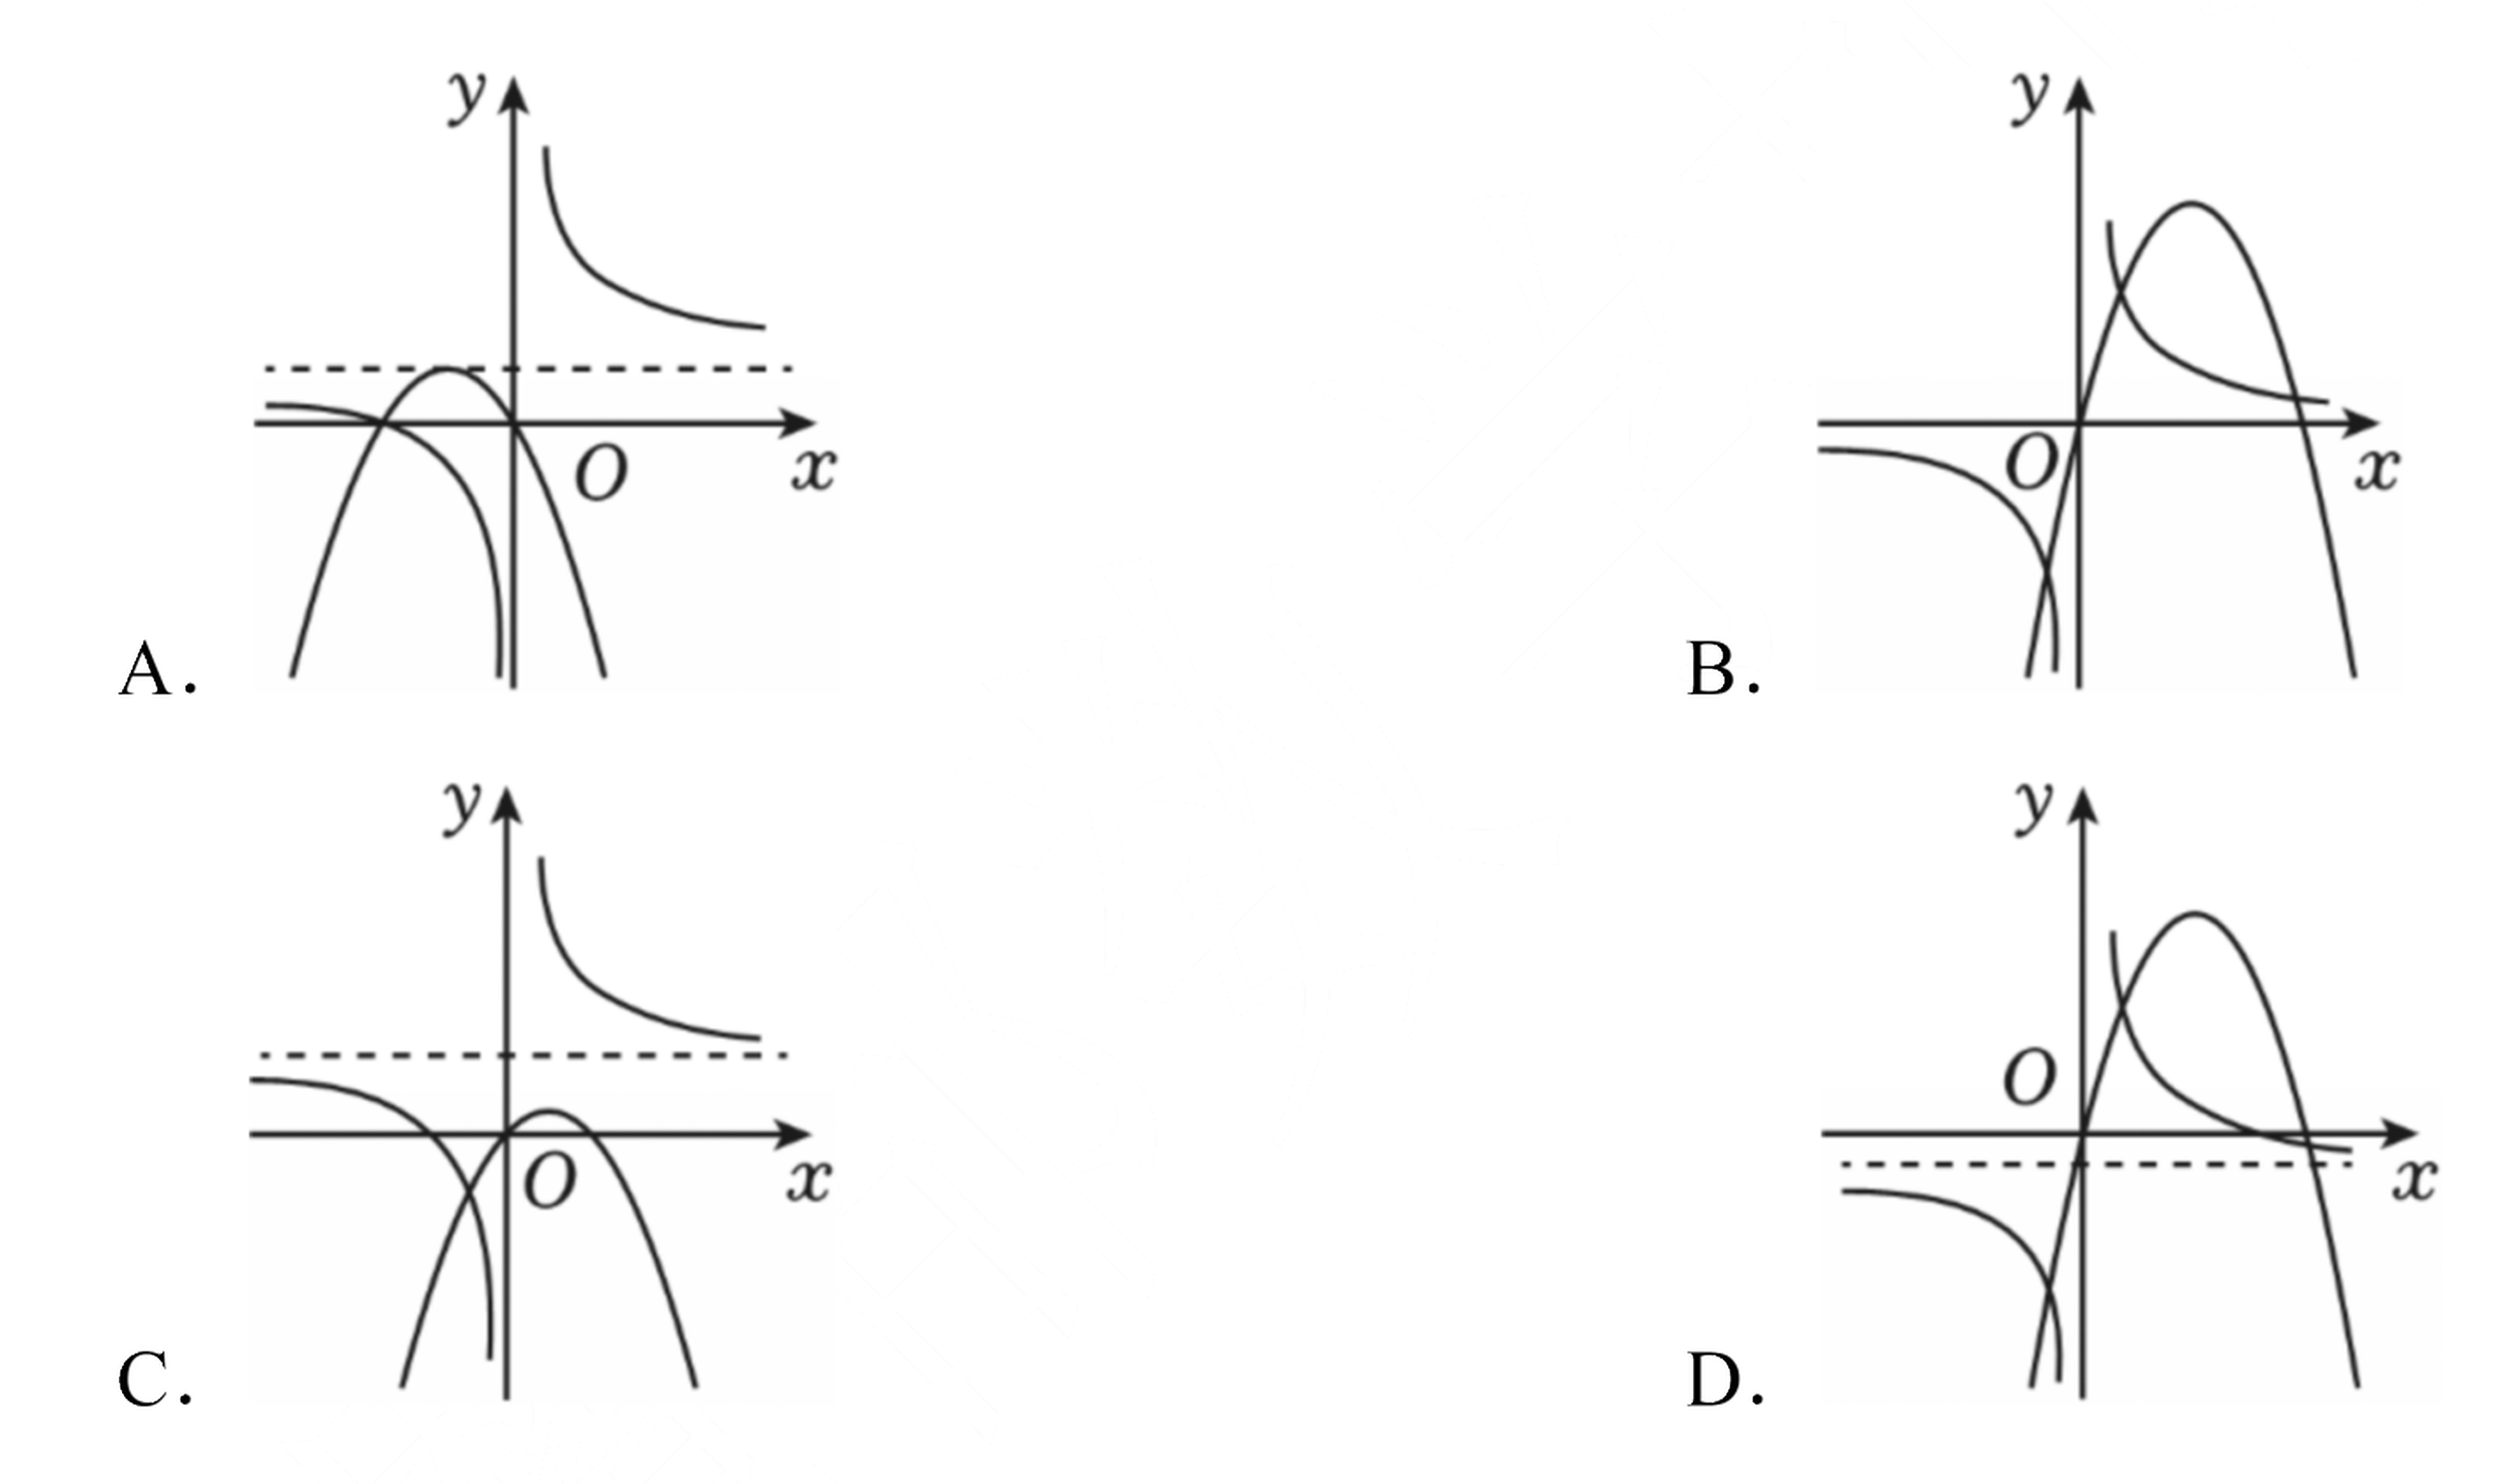
\includegraphics[width=0.80\textwidth]{figures/gao161_q14.png}
\end{center}

\ifanswer
\solbegin
\step{$A$ 选项，由二次函数图象得 $a<0$，$b<0$，由幂函数型函数图象得 $a<0$，$b>0$，}
\step{故 $A$ 选项错误；}
\step{$B$ 选项，由二次函数图象得 $a<0$，$b>0$，由幂函数型函数图象得 $a<0$，$b=0$，}
\step{故 $B$ 选项错误；}
\step{$C$ 选项，由二次函数图象得 $a<0$，$b>0$，由幂函数型函数图象得 $a<0$，$b>0$，}
\step{故 $C$ 选项正确；}
\step{$D$ 选项，由二次函数图象得 $a<0$，$b>0$，由幂函数型函数图象得 $a<0$，$b<0$，}
\step{故 $D$ 选项错误.}
\step{故选 $C$.}
\solend
\fi

% === Q15 === \subseteq／\subset、\varnothing、\mid；"排除 C""排除 B、D"正体字母照录；解析 4 行，故选 $A$
\item 设不等式 $\lvert f(x)\rvert+\lvert g(x)\rvert<a$（常数 $a>0$）的解集是 $M$，设不等式 $\lvert f(x)+g(x)\rvert<a$（常数 $a>0$）的解集是 $N$，则\mbox{（\quad）}

\keepwithprev
A. $M\subseteq N$\qquad B. $N\subseteq M$\qquad C. $M\subset N$\qquad D. $N\subset M$

\ifanswer
\solbegin
\step{$x\in M\Rightarrow\lvert f(x)+g(x)\rvert\leqslant\lvert f(x)\rvert+\lvert g(x)\rvert<a\Rightarrow x\in N$，所以 $M\subseteq N$.}
\step{取 $f(x)=g(x)=0$，则 $M=N$，排除 C.}
\step{取 $f(x)=1$，$g(x)=-1$，$a=1$，则 $M=\varnothing$，$N$ 为全体实数，排除 B、D.}
\step{故选 $A$.}
\solend
\fi

% === Q16 === "人文集"定义证明；cases 无；解析 21 行，故选 $B$
\item 设集合 $I_n=\{1,2,\cdots,n\}$，$n\in\N,n\geqslant1$，集合 $P_n=\left\{\dfrac{m}{\sqrt k}\mid m\in I_n,k\in I_n\right\}$，若 $P_n$ 的子集 $A$ 中任意两个元素之和不是整数的平方，则称 $A$ 为 “人文集”. 那么使 $P_n$ 能分成两个交集为空集的 “人文集” 的并集，且这两个人文集的并集恰为 $P_n$ 时，$n$ 的最大值是\mbox{（\quad）}

\keepwithprev
A. 13\qquad B. 14\qquad C. 15\qquad D. 16

\ifanswer
\solbegin
\step{先证当 $n\geqslant15$ 时，$P_n$ 不能分成两个不相交的人文集的并集.}
\step{假设当 $n\geqslant15$ 时，$P_n$ 可以分成两个不相交的人文集的并集，}
\step{设 $A$ 和 $B$ 为两个不相交的人文集，使 $A\cup B=P_n\supseteq I_n$.}
\step{不妨设 $1\in A$，则由于 $1+3=2^2$，所以 $3\notin A$，即 $3\in B$.}
\step{同理可得，$6\in A$，$10\in B$. 又推出 $15\in A$，}
\step{但 $1+15=4^2$，这与 $A$ 为人文集相矛盾.}
\step{再证 $P_{14}$ 满足要求. 当 $k=1$ 时，$P_{14}=\left\{\dfrac{m}{\sqrt k}\mid m\in I_{14},k\in I_{14}\right\}$，}
\step{可以分成 2 个人文集的并集.}
\step{事实上，只要取 $A_1=\{1,2,4,6,9,11,13\}$，$B_1=\{3,5,7,8,10,12,14\}$，}
\step{则 $A_1$ 和 $B_1$ 都是人文集，且 $A_1\cup B_1=P_{14}$.}
\step{当 $k=4$ 时，集合 $\left\{\dfrac{m}{\sqrt k}\mid m\in I_{14}\right\}$ 中，除整数外，}
\step{剩下的数组成集合 $\left\{\dfrac12,\dfrac32,\dfrac52,\cdots,\dfrac{13}{2}\right\}$，}
\step{可以分为下列 2 个人文集的并：$A_2=\left\{\dfrac12,\dfrac52,\dfrac92,\dfrac{11}{2}\right\}$，$B_2=\left\{\dfrac32,\dfrac72,\dfrac{13}{2}\right\}$.}
\step{当 $k=9$ 时，集合 $\left\{\dfrac{m}{\sqrt k}\mid m\in I_{14}\right\}$ 中，除整数外，}
\step{剩下的数组成集合 $\left\{\dfrac13,\dfrac23,\dfrac43,\dfrac53,\cdots,\dfrac{13}{3},\dfrac{14}{3}\right\}$，}
\step{可以分为下列 2 个人文集的并：$A_3=\left\{\dfrac13,\dfrac43,\dfrac53,\dfrac{10}{3},\dfrac{13}{3}\right\}$，$B_3=\left\{\dfrac23,\dfrac73,\dfrac83,\dfrac{11}{3},\dfrac{14}{3}\right\}$.}
\step{最后，集合 $C=\left\{\dfrac{m}{\sqrt k}\mid m\in I_{14},k\in I_{14},k\ne1,4,9\right\}$ 中的数的分母都是无理数，}
\step{它与 $P_n$ 中的任何其他数之和都不是整数，}
\step{因此，令 $A=A_1\cup A_2\cup A_3\cup C$，$B=B_1\cup B_2\cup B_3$，}
\step{则 $A$ 和 $B$ 是不相交的人文集，且 $A\cup B=P_{14}$.}
\step{综上，$n$ 的最大值为 14，故选 $B$.}
\solend
\fi

\end{enumerate}

\bigsec{三、解答题}

\begin{enumerate}
\setcounter{enumi}{16}

% === Q17 === "图像"照录；\Z；cases 块；解析 9 行，跨 06—07 页
\item (1) 已知函数 $y=x^{\frac{4m-m^2}{2}}$（$m\in\Z$）在区间 $(0,+\infty)$ 上是严格增函数，它的图像关于 $y$ 轴对称，求 $m$ 的值及该函数的解析式；

(2) 若 $(a-2)^{\frac32}<(1+2a)^{\frac32}$，求实数 $a$ 的取值范围.

\ifanswer
\solbegin
\step{(1) 由幂函数在 $(0,+\infty)$ 上严格递增，得 $\dfrac{4m-m^2}{2}>0\Leftrightarrow0<m<4$，}
\step{又 $m\in\Z$，所以 $m\in\{1,2,3\}$.}
\step{当 $m=1$ 或 $m=3$ 时，函数为 $y=x^{\frac32}$，定义域为 $[0,+\infty)$，}
\step{图像不关于 $y$ 轴对称.}
\step{当 $m=2$ 时，函数为 $y=x^2$，满足题意，所以 $m=2$，解析式 $y=x^2$.}
\step{(2) 原不等式有意义，须满足 $\begin{cases}a-2\geqslant0\\1+2a\geqslant0\end{cases}\Leftrightarrow a\geqslant2$，}
\step{函数 $y=x^{\frac32}$ 在 $[0,+\infty)$ 上严格递增，}
\step{因此 $(a-2)^{\frac32}<(1+2a)^{\frac32}\Leftrightarrow a-2<1+2a\Leftrightarrow a>-3$，}
\step{结合 $a\geqslant2$，得 $a\in[2,+\infty)$.}
\solend
\fi

% === Q18 === 题干"$a\geqslant0$"与解析"$a<0$"自相矛盾照录；"$A\cap B=(-2,-1]\cap[2,6)$"误印 ∩ 照录；\subseteq；解析 10 行
\item 已知实数 $a\geqslant0$，集合 $A=\left\{x\mid\dfrac{x+2}{x-6}<0\right\}$，$B=\{x\mid\lvert2x-1\rvert\geqslant3\}$，$C=\{x\mid x^2-3ax+2a^2<0\}$，

(1) 求 $A\cap B$；

(2) 若 $C\subseteq(A\cap B)$，求 $a$ 的取值范围.

\ifanswer
\solbegin
\step{(1) 由 $\dfrac{x+2}{x-6}<0$ 得 $-2<x<6$，即 $A=\{x\mid-2<x<6\}=(-2,6)$，}
\step{由 $\lvert2x-1\rvert\geqslant3$ 得 $2x-1\geqslant3$ 或 $2x-1\leqslant-3$，解得 $x\geqslant2$ 或 $x\leqslant-1$，}
\step{即 $B=(-\infty,-1]\cup[2,+\infty)$，}
\step{所以 $A\cap B=(-2,-1]\cap[2,6)$；}% 原卷把 ∪ 误印成 ∩，照录未改（见 ⑤ 2）
\step{(2) 由 (1) 得 $A\cap B=\{x\mid-2<x\leqslant-1\text{ 或 }2\leqslant x<6\}$，}
\step{因为 $C\subseteq(A\cap B)$，$x^2-3ax+2a^2=(x-a)(x-2a)<0$，}% 题干 $a\geqslant0$ 与解析 $a<0$ 自相矛盾，照录未改（见 ⑤ 1）
\step{当 $a=0$ 时，$C=\varnothing$，符合题意；}
\step{当 $a>0$ 时，$C=(a,2a)$，则 $\begin{cases}a\geqslant2\\2a\leqslant6\\a>0\end{cases}$，解得 $2\leqslant a\leqslant3$，}
\step{当 $a<0$ 时，$C=(2a,a)$，则 $\begin{cases}2a\geqslant-2\\a\leqslant-1\\a<0\end{cases}$，解得 $a=-1$，}
\step{故 $a$ 的范围为 $\{-1,0\}\cup[2,3]$.}
\solend
\fi

% === Q19 === 双碳太阳能应用题；"双碳""自发自用、市电互补"弯引号；解析 8 行，跨 08 页上下
\item 为响应 “双碳” 目标，某电子企业拟安装一套可使用 10 年的太阳能供电设备. 该设备的安装费用 $P(x)$（单位：万元）与太阳能电池板面积 $x(x>0)$（单位：平方米）成正比，比例系数为 $\dfrac12$. 为保障生产用电，安装后采用 “自发自用、市电互补” 模式，在此模式下，企业每年消耗的电费 $Q(x)$（单位：万元）与安装的这种太阳能电池板的面积 $x$ 之间的函数关系是 $Q(x)=\dfrac{180}{x+5}$. 记 $W(x)$（单位：万元）为该企业安装这种太阳能供电设备的费用与 10 年所消耗的电费之和.

(1) 要使该设备的安装费与第 1 年的电费之和不超过 17 万元，求安装太阳能电池板面积 $x$ 的取值范围；

(2) 当 $x$ 为多少平方米时，$W(x)$ 取得最小值？最小值是多少万元？

\ifanswer
\solbegin
\step{(1) $P(x)=\dfrac{x}{2}$，安装费与第 1 年的电费之和不超过 17 万元，即 $\dfrac{x}{2}+\dfrac{180}{x+5}\leqslant17$，}
\step{$x>0$，上式等价于 $x^2-29x+190\leqslant0\Leftrightarrow(x-10)(x-19)\leqslant0$，}
\step{解得 $x\in[10,19]$.}
\step{(2) 安装费用与 10 年电费之和为 $W(x)=P(x)+10Q(x)$，}
\step{$=\dfrac{x}{2}+\dfrac{1800}{x+5}=\dfrac{x+5}{2}+\dfrac{1800}{x+5}-\dfrac52$，}
\step{$x>0$，由基本不等式得 $W(x)\geqslant2\sqrt{\dfrac{x+5}{2}\cdot\dfrac{1800}{x+5}}-\dfrac52=60-\dfrac52=57.5$，}
\step{等号当且仅当 $\dfrac{x+5}{2}=\dfrac{1800}{x+5}$，即 $x=55$ 时成立.}
\step{因此，当电池板面积为 55 平方米时，$W(x)$ 取得最小值 57.5 万元.}
\solend
\fi

% === Q20 === $a*b$ 定义；\min 改正体；cases 块；解析 23 行，跨 08—10 页
\item 设 $a$、$b\in\R$，定义 $a*b=\begin{cases}a,&a<b\\b,&a\geqslant b\end{cases}$.

(1) 若 $x*2>1$，求 $x$ 的取值范围；

(2) 若 $(\lvert x-1\rvert+\lvert x-2\rvert)*3=3$，求 $x$ 的取值范围；

(3) 若 $a$、$b>0$，记 $M=a*\dfrac{b}{a^2+4b^2}$，分别比较 $M$ 与 $a$，以及 $M$ 与 $\dfrac{b}{a^2+4b^2}$ 的大小，并求 $M$ 的最大值.

\ifanswer
\solbegin
\step{(1) 定义 $a*b=\begin{cases}a,&a<b\\b,&a\geqslant b\end{cases}$，由 $x*2>1$，得 $\begin{cases}x<2\\x>1\end{cases}$，或 $\begin{cases}x\geqslant2\\2>1\end{cases}$，}
\step{解得 $x>1$，即 $x$ 的取值范围为 $\{x\mid x>1\}$；}
\step{(2) 当 $x\geqslant2$ 时，$\lvert x-1\rvert+\lvert x-2\rvert=2x-3\geqslant1$，}
\step{当 $1\leqslant2x-3\leqslant3$，即 $2\leqslant x\leqslant3$ 时，}
\step{此时 $(\lvert x-1\rvert+\lvert x-2\rvert)*3=2x-3=3$，解得 $x=3$；}
\step{当 $2x-3>3$，即 $x>3$ 时，}
\step{此时 $(\lvert x-1\rvert+\lvert x-2\rvert)*3=3$ 恒成立，则 $x>3$；}
\step{当 $-2x+3>3$，即 $x<0$ 时，}
\step{此时 $(\lvert x-1\rvert+\lvert x-2\rvert)*3=3$ 恒成立，则 $x<0$.}
\step{当 $1<x<2$ 时，$\lvert x-1\rvert+\lvert x-2\rvert=1$，}
\step{此时 $(\lvert x-1\rvert+\lvert x-2\rvert)*3=1\ne3$，不符合题意；}
\step{当 $x\leqslant1$ 时，$\lvert x-1\rvert+\lvert x-2\rvert=-2x+3\geqslant1$，}
\step{当 $-2x+3\leqslant3$，即 $0\leqslant x\leqslant1$ 时，}
\step{此时 $(\lvert x-1\rvert+\lvert x-2\rvert)*3=-2x+3=3$，解得 $x=0$.}
\step{综上所述，$x$ 的取值范围为 $\{x\mid x\leqslant0\text{ 或 }x\geqslant3\}$；}
\step{(3) 由题意，$M=a*\dfrac{b}{a^2+4b^2}=\min\left\{a,\dfrac{b}{a^2+4b^2}\right\}$，}% 原卷印斜体 min，按全稿惯例改正体 \min（见 ② ⑬）
\step{则 $M\leqslant a$，$M\leqslant\dfrac{b}{a^2+4b^2}$.}
\step{因为 $a$、$b>0$，所以 $\dfrac{b}{a^2+4b^2}\leqslant\dfrac{b}{2\sqrt{a^2\cdot4b^2}}=\dfrac{1}{4a}$，}
\step{当且仅当 $a=2b>0$ 时取等号，}
\step{当 $a\geqslant\dfrac{1}{4a}$，即 $a\geqslant\dfrac12$ 时，$M=a*\dfrac{b}{a^2+4b^2}=\dfrac{b}{a^2+4b^2}\leqslant\dfrac{1}{4a}$，}
\step{则 $a=\dfrac12$，$b=\dfrac14$ 时，$M$ 取得最大值 $\dfrac12$；}
\step{当 $0<a<\dfrac12$ 时，$M=a*\dfrac{b}{a^2+4b^2}=a$，此时 $M<\dfrac12$.}
\step{综上所述，$M$ 的最大值为 $\dfrac12$.}
\solend
\fi

% === Q21 === $A_n$／$B_n$／$S_n$／$T_n$ 新定义；题干第 3 问误标 (2) 照录、解析作 (3)；\prec；解析 25 行，跨 10—11 页
\item 对任意正整数 $n$，记集合 $A_n=\{(a_1,a_2,\cdots,a_n)\mid a_1,a_2,\cdots,a_n$ 均为非负整数，且 $a_1+a_2+\cdots+a_n=n\}$，集合 $B_n=\{(b_1,b_2,\cdots,b_n)\mid b_1,b_2,\cdots,b_n$ 均为非负整数，且 $b_1+b_2+\cdots+b_n=2n\}$. 设 $\alpha=(a_1,a_2,\cdots,a_n)\in A_n$，$\beta=(b_1,b_2,\cdots,b_n)\in B_n$，若对任意 $i\in\{1,2,\cdots,n\}$ 都有 $a_i\leqslant b_i$，则记 $\alpha\prec\beta$.

(1) 写出集合 $A_2$ 和 $B_2$；

(2) 证明：对任意 $\alpha\in A_n$，存在 $\beta\in B_n$，使得 $\alpha\prec\beta$；

(2) 设集合 $S_n=\{(\alpha,\beta)\mid\alpha\in A_n,\beta\in B_n,\alpha\prec\beta\}$，求证：$S_n$ 中的元素个数是完全平方数.% 原卷第 3 问题干误标 (2)（与第 2 问重号），照录未改（见 ⑤ 3）

\ifanswer
\solbegin
\step{(1) $A_2=\{(0,2),(1,1),(2,0)\}$，$B_2=\{(0,4),(1,3),(2,2),(3,1),(4,0)\}$；}
\step{(2) 对任意 $\alpha=(a_1,a_2,\cdots,a_n)\in A_n$，设 $b_i=a_i+1$（$i=1,2,3,\cdots,n$），}
\step{则 $b_1,b_2,\cdots,b_n$ 均为非负整数，且 $a_i\leqslant b_i$（$i=1,2,3,\cdots,n$）.}
\step{令 $\beta=(b_1,b_2,\cdots,b_n)$，则 $b_1+b_2+\cdots+b_n$}
\step{$=(a_1+1)+(a_2+1)+\cdots+(a_n+1)=(a_1+a_2+\cdots+a_n)+n=2n$，}
\step{所以 $\beta\in B_n$，且 $\alpha\prec\beta$.}
\step{(3) 对任意 $\alpha=(a_1,a_2,\cdots,a_n)\in A_n$，$\alpha'=(a_1',a_2',\cdots,a_n')\in A_n$，}
\step{记 $\alpha+\alpha'=(a_1+a_1',a_2+a_2',\cdots,a_n+a_n')$，}
\step{则 $a_1+a_1',a_2+a_2',\cdots,a_n+a_n'$ 均为非负整数，}
\step{且 $(a_1+a_1')+(a_2+a_2')+\cdots+(a_n+a_n')$}
\step{$=(a_1+a_2+\cdots+a_n)+(a_1'+a_2'+\cdots+a_n')=n+n=2n$，}
\step{所以 $\alpha+\alpha'\in B_n$，且 $\alpha\prec\alpha+\alpha'$，$\alpha'\prec\alpha+\alpha'$.}
\step{设集合 $A_n$ 中的元素个数为 $t$，设 $A_n=\{\alpha_1,\alpha_2,\cdots,\alpha_t\}$.}
\step{设集合 $T_n=\{(\alpha_i,\alpha_i+\alpha_j)\mid i=1,2,\cdots,t,j=1,2,\cdots,t\}$.}
\step{对任意 $\alpha_i\in A_n$（$i=1,2,\cdots,t$），都有 $\alpha_i+\alpha_1,\alpha_i+\alpha_2,\cdots,\alpha_i+\alpha_t\in B_n$，}
\step{且 $\alpha_i\prec\alpha_i+\alpha_j$，$j=1,2,\cdots,t$，所以 $T_n\subseteq S_n$.}
\step{若 $(\alpha,\beta)\in S_n$，其中 $\alpha=(a_1,a_2,\cdots,a_n)\in A_n$，$\beta=(b_1,b_2,\cdots,b_n)\in B_n$，}
\step{设 $c_i=b_i-a_i$（$i=1,2,\cdots,n$），因为 $a_i\leqslant b_i$，所以 $c_i=b_i-a_i\geqslant0$，}
\step{记 $\alpha'=(c_1,c_2,\cdots,c_n)$，}
\step{则 $c_1+c_2+\cdots+c_n=(b_1-a_1)+(b_2-a_2)+\cdots+(b_n-a_n)$}
\step{$=(b_1+b_2+\cdots+b_n)-(a_1+a_2+\cdots+a_n)=2n-n=n$，}
\step{所以 $\alpha'\in A_n$，并且有 $\beta=\alpha+\alpha'$，所以 $(\alpha,\beta)\in T_n$，所以 $S_n\subseteq T_n$，}
\step{所以 $S_n=T_n$.}
\step{因为集合 $T_n$ 中的元素个数为 $t^2$，所以 $S_n$ 中的元素个数为 $t^2$，}
\step{是完全平方数.}
\solend
\fi

\end{enumerate}

\end{document}
"
% 紧凑版：xelatex "\def\iscompact{1}% 高一161_松江一中嘉一实验_期中.tex
%   —— 高一上数学"2026-2027 年松江一中嘉一实验高一上期中"（试卷版/答案版/紧凑版）
% 试卷版：xelatex 高一161_松江一中嘉一实验_期中.tex
% 答案版：xelatex "\def\isanswer{1}% 高一161_松江一中嘉一实验_期中.tex
%   —— 高一上数学"2026-2027 年松江一中嘉一实验高一上期中"（试卷版/答案版/紧凑版）
% 试卷版：xelatex 高一161_松江一中嘉一实验_期中.tex
% 答案版：xelatex "\def\isanswer{1}\input{高一161_松江一中嘉一实验_期中.tex}"
% 紧凑版：xelatex "\def\iscompact{1}\input{高一161_松江一中嘉一实验_期中.tex}"
%
% ① 原始材料：微信公众号"魔都数学加油站"文章，连载"27学年高一161"，原卷卷面标题
% "2026-2027 年松江一中嘉一实验高一上期中"（卷面未印副标题、未印连载号）。
% 正文为 11 张 PNG 页（01/02/03/05/06/07/08/09/11 为 4762×6735，04/10 为
% 2560×3620，同一篇各页分辨率混排，逐页按各自分辨率裁图核对）。
% 体例：讲评版——填空 3—12（10 题）、选择 13—16（4 题）、解答 17—21（5 题），
% 共 19 题，自第 3 题起编（1、2 未印在本篇）；Q13 答案"A"直接印在题干括号内、
% 且无【答案】/【解析】段，本稿按 高一37 第 13 题／高一57 第 13 题成例把括号
% 留空、另提 \ans{$A$}；其余 18 题逐题印【解析】、用 \solbegin…\solend。
% 题目、答案、解析均据原图转录；卷面粉红色水印"魔都数学加油站"及公众号页脚未录入。
% 全卷插图清单（逐页通读 11 页确认）：仅 1 组——Q14 四幅图像选项（04 页 2×2
% 排布，二次函数与幂函数型函数在同一坐标系中的图象，A/B/C/D 四幅小图），
% 合并成一张，三版都出，裁 figures/gao161_q14.png。其余各页逐页确认无其它
% 题目配图、无解析内配图、无表格、无"如图"处（Q16 解析里的"可以分为下列 2 个
% 人文集的并"是纯文字＋集合，不是表格；OCR 里看似表格的行实为大括号与分数）。
%
% 卷首标题：原卷印作"2026-2027 年松江一中嘉一实验高一上期中"，年份区间按全稿惯例排 en dash；
% 原卷卷面未印副标题，本稿按同期中卷知识模块口径补出"集合与常用逻辑用语、不等式、函数"。
%
% ② 与原卷的排版差异／照录项清单：
%   ① 原文从第 3 题起，本稿保留原题号；共 19 题三节，解答题 5 题到 21；
%      三节各自一个 enumerate + \setcounter{enumi}{2}/{12}/{16}（不贯穿），
%      用 \examtitlest[3] 起手；
%   ② 混合体例：Q13 原卷把答案"A"直接印在题干括号内（"（  A  ）"）、且题下
%      无【答案】/【解析】段，按 高一37 第 13 题／高一57 第 13 题成例把括号
%      留空、另提 \ans{$A$}、不补造解析；其余 18 题印【解析】、用
%      \solbegin…\solend；四道选择题中 Q14/Q15/Q16 的答案在解析末句
%      "故选 $C$／$A$／$B$"、Q13 用 \ans{$A$}；括号 \mbox{（\quad）} 留空；
%      答案版【答案】/【解析】标记数 = 19 = 全卷题数（1 个 \ans ＋ 18 个 \solbegin）；
%   ③ 原卷卷面未印副标题，本稿按知识模块口径补出；
%   ④ 原卷填空横线按全稿惯例排 \blankline[4.4em]；选择题选项段前按惯例各加
%      \keepwithprev；Q14 四幅选项图整块用 \needvspace{9cm} 守卫（守卫放
%      \item 之前，见 高一132 Q14／高一154 Q15 成例）；解答题不留作答区、
%      不加 \anspace（原卷为讲评版）；
%   ⑤ 数集归一：Q8"$x\in\R$"、Q11"$m\in\R$"、Q13"$x,y\in\N$"、
%      Q16"$n\in N$"、Q17"$m\in\Z$"、Q20"$a$、$b\in R$"——原卷印正体粗体
%      或斜体 R/N/Z，按全稿惯例归一 \R／\N／\Z；绝对值排 \lvert…\rvert
%      （Q9、Q12、Q15、Q18、Q20），集合描述竖线排 \mid（Q12、Q16、Q18、
%      Q20、Q21），空集 \varnothing（Q15、Q18），补集无用例，不等号按全稿
%      惯例排 \leqslant／\geqslant；
%   ⑥ 子集符号逐处照录不统一：Q12 cases 定义"$C(A)\geqslant C(B)$"、
%      Q15 选项 A/B"$M\subseteq N$""$N\subseteq M$"与解析"$M\subseteq N$"
%      印带下划线 ⊆（照录 \subseteq），Q15 选项 C/D"$M\subset N$""$N\subset M$"
%      印单线 ⊂（照录 \subset），Q18 "$C\subseteq(A\cap B)$"、Q21
%      "$T_n\subseteq S_n$""$S_n\subseteq T_n$"均带下划线照录 \subseteq；
%      本卷无 \not\subset 用例；
%   ⑦ 判别式：Q7 解析"$\Delta=(m-6)(m+2)>0$"、Q8 解析"$\Delta=a^2-4a<0$"、
%      Q12 解析"$\Delta=a^2-8$"共 3 处，逐处放大确认印等腰偏高粗三角
%      （高>宽、右斜边粗），照录 \Delta；本卷无扁等边细线 \triangle 用例；
%   ⑧ 中文弯引号照录：Q7"$m\geqslant6$""有两个不相等的正实数根"及四个
%      条件短语、Q13 反证法命题、Q16"人文集"、Q19"双碳""自发自用、市电互补"；
%      注释里一律 ASCII 引号；数学式内 CJK 用 \text{}（Q18、Q20 解集描述内"或"）；
%   ⑨ "图像／图象"逐处照录不统一：Q4"的图像"、Q17 题干"它的图像关于 $y$ 轴
%      对称"及解析"图像不关于 $y$ 轴对称"印"图像"；Q14 题干"的图象可能为"
%      与解析 A/B/C/D 四行各"由二次函数图象得""由幂函数型函数图象得"
%      共 8 处印"图象"（象，无亻）；
%   ⑩ 文本圈数字逐处照录：Q12 题干①②③④、Q12 解析"故①错误""故②正确"
%      "故③正确""故④错误""故正确的是②③"，均为印刷圈数字（文本模式）；
%   ⑪ 半角逗号在数学组之间是全稿惯例、非笔误，逐处照录（Q5"$a$、$b$"、
%      Q13"$x,y\in\N$"、Q16"$n\in\N,n\geqslant1$"与集合描述内逗号、
%      Q20"$a,b\in\R$"、Q21 各集合描述内逗号）；行末西文句点 ASCII `.`；
%      原卷行中句点（Q16"$10\in B$. 又推出 $15\in A$"、Q16"再证 $P_{14}$
%      满足要求. 当 $k=1$ 时"、Q18"$A\cap B=(-2,-1]\cap[2,6)$；"后的分号）
%      按全稿惯例一律排 ASCII `.`／全角"；"；中文语境行中全角逗号／顿号照录；
%   ⑫ 原卷数学式内联条件（Q14"$y=x^a+b(a\ne0)$"、Q19"$x(x>0)$"、
%      Q11"$\lvert x-m\rvert<n\,(m\in\R,n>0)$"）印半角括号，逐处照录未改
%      全角（同 高一147 口径）；
%      中文语境的括注（Q5"结果用 $a$、$b$ 表示"、Q7"填…"、Q12"填写序号"、
%      Q15"常数 $a>0$"、Q19"单位：万元"）印全角括号，照录；
%   ⑬ 复杂式照录别简化：Q3 $(a^{2-\sqrt3})^{2+\sqrt3}\times\sqrt{a^2}\times
%      b^{\sqrt3}\times b^{1-\sqrt3}$ 与 $a^{(2-\sqrt3)(2+\sqrt3)}\cdot a\cdot
%      b^{\sqrt3+1-\sqrt3}=a\cdot a\cdot b=a^2b$（题干用 \times、解析用 \cdot，
%      逐处照录不统一，见 ⑤）；Q5 $\dfrac{\lg2}{\lg2+\lg3}=\dfrac{a}{a+b}$、
%      Q10 $t-\dfrac3t=2$ 与 $b=a^3$、$ab=a^4=2$、Q11 $\left(2a-\dfrac12
%      -a+\dfrac12,2a-\dfrac12+a-\dfrac12\right)=(a,3a-1)$ 与
%      $\left(\dfrac43,\dfrac53\right]\cup\{2\}$、Q16 各分数集合、Q19
%      $x^2-29x+190\leqslant0$ 与 $W(x)=P(x)+10Q(x)$ 与
%      $2\sqrt{\dfrac{x+5}{2}\cdot\dfrac{1800}{x+5}}-\dfrac52=60-\dfrac52=57.5$、
%      Q20 $M=a*\dfrac{b}{a^2+4b^2}=\min\left\{a,\dfrac{b}{a^2+4b^2}\right\}$
%      与 $\dfrac{b}{2\sqrt{a^2\cdot4b^2}}=\dfrac{1}{4a}$、Q21 各 $A_n$／$B_n$／
%      $T_n$ 定义；\left…\right 不得拆到不同 $…$ 组（Q11 的 \left(…\right)、
%      Q11 的 \left(\dfrac43,\dfrac53\right]、Q16 的 \left\{\dfrac{m}{\sqrt k}
%      \mid…\right\} 与 \left\{\dfrac12,\dfrac32,\dfrac52,\cdots,\dfrac{13}{2}\right\}
%      等、Q20 的 \min\left\{…\right\}）；cases 块整体算一个印刷行
%      （Q12 定义、Q17 (2)、Q18 (2) 两处、Q20 定义与 (1)）；原卷 Q20 解析
%      "$=min\{…\}$"印斜体 min，按 高一122／高一102 成例改正体 \min；
%   ⑭ 一条 \step = 原卷解析的一个印刷行；别并折行、别拆行。跨页续印按题合并
%      （Q6 的 01 页上下题干重复印、Q10 的 01—02 页、Q11 的 02—03 页、
%      Q12 的 03—04 页、Q16 的 05—06 页、Q17 的 06—07 页、Q18 的 07 页
%      上下、Q19 的 08 页上下、Q20 的 08—10 页、Q21 的 10—11 页）；
%      跨半页重叠行（Q10"令 $t=\log_a b>0$…"、Q16"它与 $P_n$ 中的任何
%      其他数之和都不是整数，"、Q18"【解析】(1) 由 $\dfrac{x+2}{x-6}<0$…"、
%      Q19"$x>0$，上式等价于…"、Q20"此时…则 $x<0$."、Q21"若 $(\alpha,\beta)
%      \in S_n$…"与"设 $c_i=b_i-a_i$…"）只算一个印刷行；
%   ⑮ 自定义记号照录：Q12"$C(A)$""$A*B$""$S$"、Q16"$I_n$""$P_n$""人文集"
%      "$A_1$／$B_1$／$A_2$／$B_2$／$A_3$／$B_3$／$C$"、Q20"$a*b$""$M$"、
%      Q21"$A_n$／$B_n$／$S_n$／$T_n$""$\alpha\prec\beta$""$\alpha+\alpha'$"；
%   ⑯ 选项字母体例照录不统一：Q15 解析"排除 C.""排除 B、D."两处原卷印
%      正体（文本模式），Q13 \ans{$A$}、Q14"$A$ 选项"…"故选 $C$"、
%      Q15"故选 $A$"、Q16"故选 $B$"用斜体（数学模式），逐处照录、不统一；
%   ⑰ 红字：全卷逐页扫描无红色加粗小标题（仅粉色水印），故本卷无 \stepm，
%      不引入红色定义；
%
% ③ 行数复核：一条 \step = 原卷解析的一个印刷行，cases 块作一个印刷行计。
%   逐题数（逐页核对定稿）：Q3：1；Q4：1；Q5：1；Q6：3；Q7：4；Q8：4；
%   Q9：2；Q10：2；Q11：7；Q12：8；Q13：0（答案印括号内、提 \ans{}，
%   不计入 \step 账）；Q14：9；Q15：4；Q16：21；Q17：9；Q18：10；Q19：8；
%   Q20：23；Q21：25。
%   合计 142 行（142 条 \step，无 \stepm），与原卷逐题印刷行相等。
%   全卷 19 题：Q13 一处 \ans{} ＋ 其余 18 题设 \solbegin…\solend，
%   答案版【答案】/【解析】标记数 = 19 = 全卷题数。
%
% ④ 页码分布（供回原图复核）：
%   卷首标题＋"一、填空题"＋Q3/Q4/Q5 题干＋解析各 1 行＋Q6 题干首行
%   在 01 页上半；Q6 题干（重复印）＋解析 3 行＋Q7 题干＋解析 4 行在
%   01 页下半；Q8 题干＋解析 4 行＋Q9 题干＋解析 2 行＋Q10 题干＋
%   解析首行在 02 页上半；Q10 解析（重复印）＋末行＋Q11 题干＋解析
%   前 3 行在 02 页下半；Q11 解析后 4 行＋Q12 题干＋cases 定义＋①
%   在 03 页上半；Q12 ②③④ 三命题＋"填写序号"行＋解析前 6 行在
%   03 页下半；Q12 解析后 2 行＋"二、选择题"标题＋Q13 题干＋选项＋
%   Q14 题干＋"（　）"＋A/B 两幅图在 04 页上半；Q14 四幅图（重复印）
%   ＋解析 9 行在 04 页下半；Q15 题干＋选项＋解析 4 行＋Q16 题干＋
%   选项在 05 页上半；Q16 题干（重复印）＋选项＋解析前 10 行在 05 页
%   下半；Q16 解析中 8 行（k=4、k=9 两批＋集合 C＋"它与 $P_n$…"）
%   在 06 页上半；Q16 解析"它与 $P_n$…"（重复印）＋末 3 行＋
%   "三、解答题"标题＋Q17 题干＋两问＋解析前 4 行在 06 页下半；
%   Q17 解析后 5 行＋Q18 题干＋两问＋解析首行在 07 页上半；Q18 解析
%   （重复首行）＋余 9 行在 07 页下半；Q19 题干＋两问＋解析前 2 行在
%   08 页上半；Q19 解析（重复第 2 行）＋余 6 行＋Q20 定义＋(1) 问在
%   08 页下半；Q20 (2)(3) 两问＋解析 (1) 2 行＋(2) 前 7 行在 09 页
%   上半；Q20 解析 (2) 余 4 行＋(3) 前 4 行在 09 页下半；Q20 解析 (3)
%   余 4 行＋Q21 题干＋三问在 10 页上半；Q21 题干（重复印）＋解析
%   (1)(2)(3) 前 8 行在 10 页下半；Q21 解析 (3) 中 10 行在 11 页上半；
%   Q21 解析 (3)（重复 2 行）＋末 7 行"是完全平方数."在 11 页下半。
%   本稿按题连排，不丢行、不并折行；全卷末题为第 21 题，无附加题节。
%
% ⑤ 存疑照录（放大原图确认，照录未改、正文对应处另有 % 注）：
%   1. Q18 题干印"已知实数 $a\geqslant0$"，解析却另设"当 $a<0$ 时"并解出
%      $a=-1$，末行答案"故 $a$ 的范围为 $\{-1,0\}\cup[2,3]$"含负数，
%      与题干 $a\geqslant0$ 自相矛盾——系原卷前后不一，照录未改（放大
%      07 页确认题干确印 $a\geqslant0$）；
%   2. Q18 解析"所以 $A\cap B=(-2,-1]\cap[2,6)$；"原卷把并集误印成
%      交集号 ∩（紧接下一行"$A\cap B=\{x\mid-2<x\leqslant-1$ 或
%      $2\leqslant x<6\}$"用"或"），照录未改（放大 07 页确认印 ∩）；
%   3. Q21 题干第 3 问原卷标号印作"(2)"（与第 2 问重号），而解析里
%      同一问标作"(3)"——原卷笔误，题干与解析逐处照录、不统一；
%   4. Q3 题干四处乘号印"×"（\times）、解析内三处乘号印"·"（\cdot），
%      逐处照录未统一（放大 01 页确认）；
%   5. Q16 解析"先证当 $n\geqslant15$ 时"印 ≥（非 >），与"综上，$n$
%      的最大值为 14"自洽，照录；题干"$n\in N,n\geqslant1$"印斜体
%      $N$、按全稿惯例归一 \N（见 ② ⑤）；
%   6. Q20 解析"$M=a*\dfrac{b}{a^2+4b^2}=min\{…\}$"原卷印斜体 min，
%      按全稿惯例改正体 \min（见 ② ⑬）；末行"$M$ 的最大值为
%      $\dfrac12$"照录；
%   7. Q15 解析"排除 C.""排除 B、D."用正体字母，而"故选 $A$"用斜体
%      字母，原卷体例不一（见 ② ⑯），照录未统一。
%   全卷除此 7 类外未发现其它笔误／自相矛盾处；Q13 只把答案印在括号内、
%   其余 18 题全部印【解析】。
%

\documentclass[a4paper,11pt]{article}
\usepackage{common}

\begin{document}

\examtitlest[3]{2026--2027 年松江一中嘉一实验高一上期中}{集合与常用逻辑用语、不等式、函数}

\bigsec{一、填空题}

\begin{enumerate}
\setcounter{enumi}{2}

% === Q3 === 题干 \times、解析 \cdot 逐处照录；解析 1 行
\item 设 $a>0$，$b>0$，化简 $(a^{2-\sqrt3})^{2+\sqrt3}\times\sqrt{a^2}\times b^{\sqrt3}\times b^{1-\sqrt3}=$\blankline[4.4em].

\ifanswer
\solbegin
\step{因为 $a>0$，所以 $\sqrt{a^2}=a$，原式 $=a^{(2-\sqrt3)(2+\sqrt3)}\cdot a\cdot b^{\sqrt3+1-\sqrt3}=a\cdot a\cdot b=a^2b$.}
\solend
\fi

% === Q4 === "图像"照录；解析 1 行
\item 若幂函数 $y=x^a$ 的图像经过点 $(5,\sqrt5)$，则此幂函数的表达式为 $y=$\blankline[4.4em].

\ifanswer
\solbegin
\step{$5^a=\sqrt5\Rightarrow a=\dfrac12$，所以 $y=\sqrt x$.}
\solend
\fi

% === Q5 === "结果用 $a$、$b$ 表示"全角括号＋顿号照录；解析 1 行
\item 已知 $\lg2=a$，$10^b=3$，则 $\log_6 2=$\blankline[4.4em]（结果用 $a$、$b$ 表示）.

\ifanswer
\solbegin
\step{$\lg3=b$，$\log_6 2=\dfrac{\lg2}{\lg2+\lg3}=\dfrac{a}{a+b}$.}
\solend
\fi

% === Q6 === 对称中心；解析 3 行，题干跨 01 页上下重复印
\item 若函数 $y=\dfrac{mx-1}{x+n}$ 的对称中心是 $(4,-3)$，则 $m+n=$\blankline[4.4em].

\ifanswer
\solbegin
\step{令 $x=-n+t$（$t\ne0$），则 $y-m=-\dfrac{mn+1}{t}$；}
\step{将 $t$ 换成 $-t$，$y-m$ 变为其相反数，因此对称中心为 $(-n,m)$.}
\step{于是 $n=-4$，$m=-3$，得 $m+n=-7$.}
\solend
\fi

% === Q7 === 充要条件；中文弯引号＋圈选条件；\Delta 高瘦；解析 4 行
\item 已知关于 $x$ 的一元二次方程 $x^2-mx+m+3=0$，则 “$m\geqslant6$” 是该方程 “有两个不相等的正实数根” 的\blankline[4.4em]条件（填 “充分不必要”、“必要不充分”、“充要” 或 “既不充分也不必要”）.

\ifanswer
\solbegin
\step{方程有两个不相等的正实数根}
\step{$\Leftrightarrow m>0$、$m+3>0$ 且 $\Delta=(m-6)(m+2)>0\Leftrightarrow m>6$.}
\step{$m>6\Rightarrow m\geqslant6$，但 $m=6$ 时方程有两个相等的正实数根，}
\step{因此为必要不充分条件.}
\solend
\fi

% === Q8 === \R、\Delta；解析 4 行
\item 对于任意的 $x\in\R$，代数式 $\lg(ax^2+ax+1)$ 都有意义，则实数 $a$ 的取值范围是\blankline[4.4em].

\ifanswer
\solbegin
\step{真数须满足 $ax^2+ax+1>0$ 对任意 $x\in\R$ 恒成立.}
\step{$a=0$ 时成立；}
\step{$a\ne0$ 时，恒成立等价于 $a>0$ 且 $\Delta=a^2-4a<0$，解得 $0<a<4$；}
\step{因此 $a\in[0,4)$.}
\solend
\fi

% === Q9 === 绝对值 \lvert…\rvert；解析 2 行
\item 若不等式 $\lvert x+1\rvert-\lvert x-4\rvert<m$ 的解集为非空集合，则实数 $m$ 的取值范围是\blankline[4.4em].

\ifanswer
\solbegin
\step{$\lvert x+1\rvert-\lvert x-4\rvert\geqslant-\lvert(x+1)-(x-4)\rvert=-5$，当 $x=-1$ 时取等号，}
\step{因此原不等式的解集非空 $\Leftrightarrow m>-5$，所求范围为 $(-5,+\infty)$.}
\solend
\fi

% === Q10 === 换底；$\log_2 a\cdot\log_2 b$；解析 2 行，跨 02 页上下
\item 已知 $a>1$，$b>1$，若 $\log_a b-3\log_b a=2$，且 $ab=2$，则 $\log_2 a\cdot\log_2 b=$\blankline[4.4em].

\ifanswer
\solbegin
\step{令 $t=\log_a b>0$，则 $t-\dfrac{3}{t}=2\Leftrightarrow(t-3)(t+1)=0$，得 $t=3$，}
\step{于是 $b=a^3$，$ab=a^4=2$，得 $\log_2 a=\dfrac14$，$\log_2 b=\dfrac34$，所求为 $\dfrac{3}{16}$.}
\solend
\fi

% === Q11 === 邻域定义；\left(…\right) 不拆组；解析 7 行，跨 02—03 页
\item 对于实数 $m$ 和正数 $n$，称满足不等式 $\lvert x-m\rvert<n\,(m\in\R,n>0)$ 的实数 $x$ 的集合叫做 $m$ 的 $n$ 邻域. 已知 $a>\dfrac12$，若 $2a-\dfrac12$ 的 $a-\dfrac12$ 邻域中恰有 2 个整数，则 $a$ 的取值范围是\blankline[4.4em].

\ifanswer
\solbegin
\step{所求邻域为 $\left(2a-\dfrac12-a+\dfrac12,2a-\dfrac12+a-\dfrac12\right)=(a,3a-1)$.}
\step{当 $\dfrac12<a\leqslant1$ 时至多含 1 个整数；}
\step{当 $a>2$ 时，区间长度 $2a-1>3$，至少含 3 个整数.}
\step{当 $1<a<2$ 时，区间必含 2，恰有两个整数等价于 $3<3a-1\leqslant4$，}
\step{即 $\dfrac43<a\leqslant\dfrac53$.}
\step{当 $a=2$ 时，区间为 $(2,5)$，恰含整数 $3,4$；}
\step{所以 $a\in\left(\dfrac43,\dfrac53\right]\cup\{2\}$.}
\solend
\fi

% === Q12 === $C(A)$／$A*B$ 定义题；①②③④ 文本圈数字；\subseteq／\subset、\Delta、\mid、\varnothing；解析 8 行
\item 用 $C(A)$ 表示非空集合 $A$ 中的元素个数. 对于集合 $A$、$B$，定义

$A*B=\begin{cases}C(A)-C(B),&C(A)\geqslant C(B)\\ C(B)-C(A),&C(A)<C(B)\end{cases}$，若 $A=\{0,1\}$，$B=\{x\mid(x^2-ax)(x^2+ax+2)=0\}$，设实数 $a$ 的所有可能取值组成的集合是 $S$，则下列说法正确的是\blankline[4.4em]（填写序号）.

① $C(B)$ 的可能值为 $2,3,4$

② 若 $A*B=2$，则 $a$ 的取值范围为 $(-\infty,-2\sqrt2)\cup(2\sqrt2,+\infty)$

③ 若 $A*B=1$，则 $C(S)=3$

④ 若 $A*B=0$，则 $a$ 的取值范围为 $(-2\sqrt2,2\sqrt2)$

\ifanswer
\solbegin
\step{$x(x-a)=0$ 的根为 $0,a$，而 $x^2+ax+2$ 在这两处的值分别为 $2,2a^2+2$，}
\step{两个因式无公共实根；后者的判别式为 $\Delta=a^2-8$.}
\step{当 $a=0$、$0<\lvert a\rvert<2\sqrt2$、$\lvert a\rvert=2\sqrt2$、$\lvert a\rvert>2\sqrt2$ 时，$C(B)$ 依次为 $1,2,3,4$，}
\step{故①错误.}
\step{$A*B=\lvert2-C(B)\rvert$，所以 $A*B=2\Leftrightarrow\lvert a\rvert>2\sqrt2$，故②正确；}
\step{$A*B=1\Leftrightarrow a\in\{-2\sqrt2,0,2\sqrt2\}$，此时 $C(S)=3$，故③正确；}
\step{$A*B=0\Leftrightarrow0<\lvert a\rvert<2\sqrt2$，即 $a\in(-2\sqrt2,0)\cup(0,2\sqrt2)$，故④错误.}
\step{故正确的是②③.}
\solend
\fi

\end{enumerate}

\needvspace{7cm}
\bigsec{二、选择题}

\begin{enumerate}
\setcounter{enumi}{12}

% === Q13 === 答案"A"原卷印在题干括号内、题下无【答案】/【解析】段；按 高一37／高一57 成例另提 \ans{}
\item 用反证法证明命题 “已知 $x>0$，$y>0$，$x,y\in\N$，如果 $xy$ 可被 7 整除，那么 $x$，$y$ 至少有一个能被 7 整除” 时，假设的内容是\mbox{（\quad）}

\keepwithprev
A. $x$、$y$ 都不能被 7 整除\qquad B. $x$、$y$ 都能被 7 整除

C. $x$、$y$ 只有一个能被 7 整除\qquad D. 只有 $x$ 不能被 7 整除

\ifanswer
\ans{$A$}
\fi

% === Q14 === 四幅图像选项（2×2 合并，三版都出）；守卫放 \item 之前；"图象"照录；解析 9 行，故选 $C$
\needvspace{9cm}
\item 函数 $y=ax^2+bx$ 与函数 $y=x^a+b(a\ne0)$ 在同一平面直角坐标系中的图象可能为\mbox{（\quad）}

\keepwithprev
\begin{center}
% 四幅图象选项取 04 页 2×2 排布合并为一张，去粉色水印、转灰度、4× LANCZOS 放大；三版都出
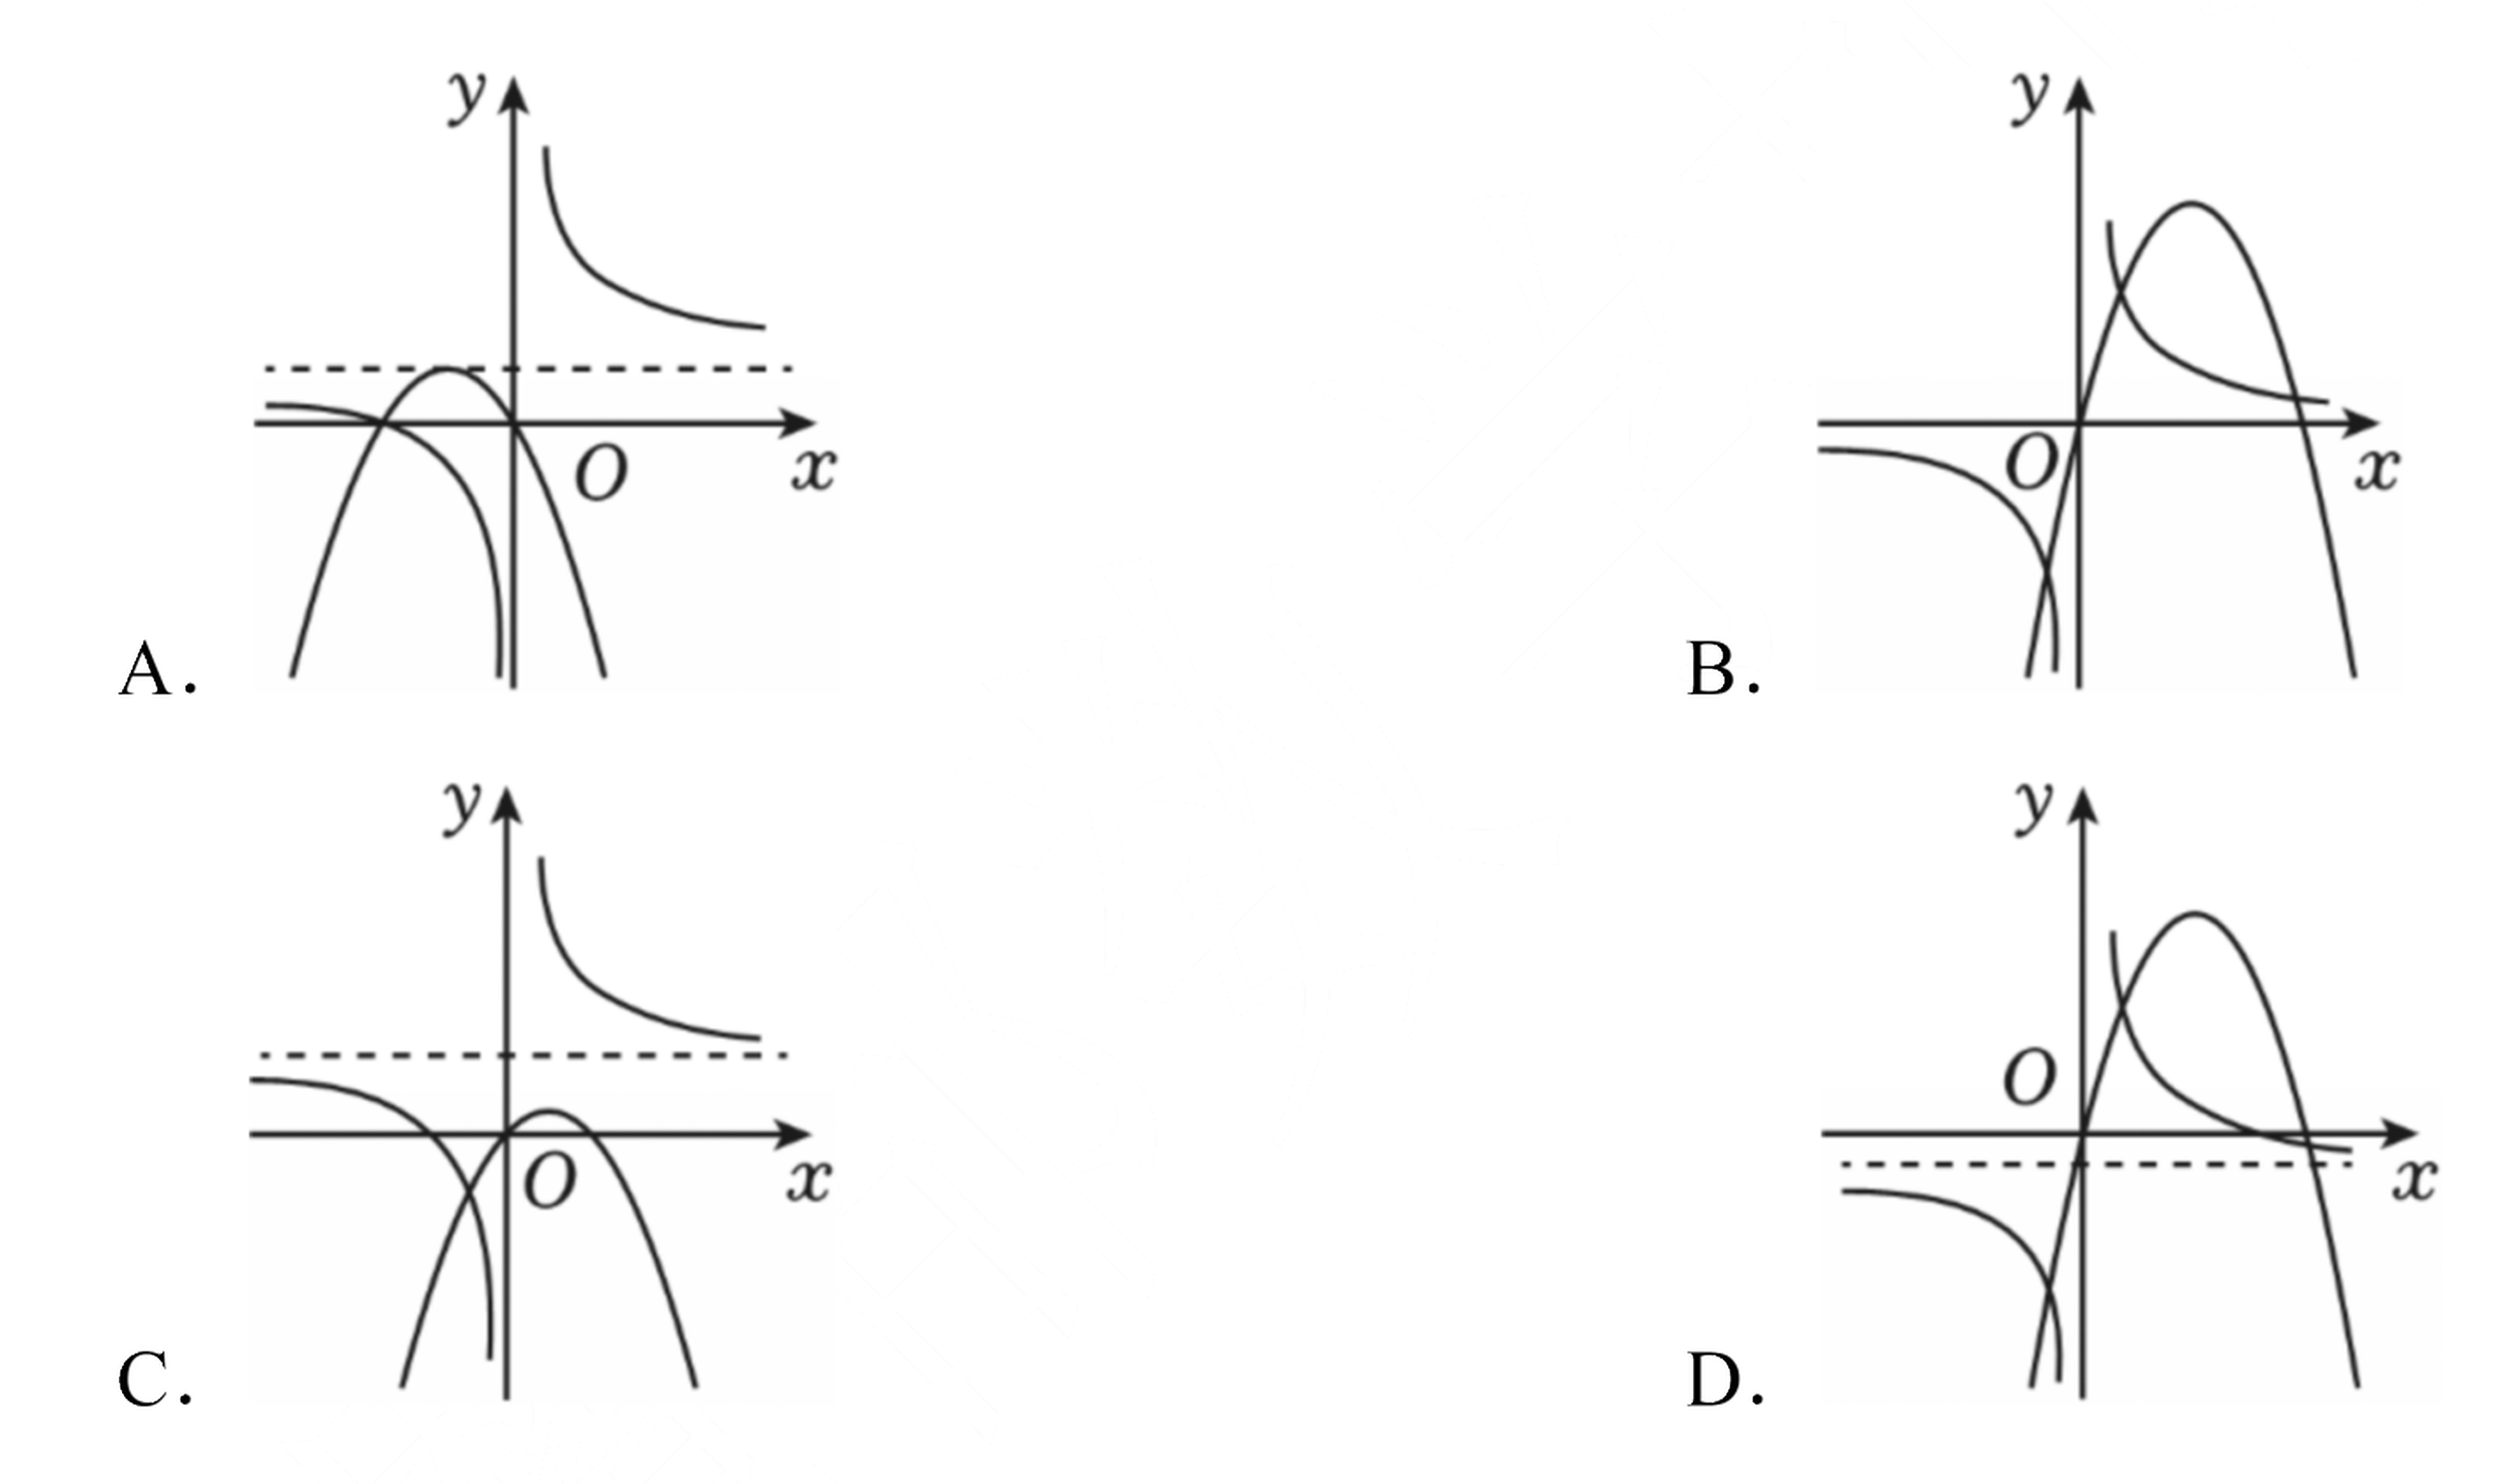
\includegraphics[width=0.80\textwidth]{figures/gao161_q14.png}
\end{center}

\ifanswer
\solbegin
\step{$A$ 选项，由二次函数图象得 $a<0$，$b<0$，由幂函数型函数图象得 $a<0$，$b>0$，}
\step{故 $A$ 选项错误；}
\step{$B$ 选项，由二次函数图象得 $a<0$，$b>0$，由幂函数型函数图象得 $a<0$，$b=0$，}
\step{故 $B$ 选项错误；}
\step{$C$ 选项，由二次函数图象得 $a<0$，$b>0$，由幂函数型函数图象得 $a<0$，$b>0$，}
\step{故 $C$ 选项正确；}
\step{$D$ 选项，由二次函数图象得 $a<0$，$b>0$，由幂函数型函数图象得 $a<0$，$b<0$，}
\step{故 $D$ 选项错误.}
\step{故选 $C$.}
\solend
\fi

% === Q15 === \subseteq／\subset、\varnothing、\mid；"排除 C""排除 B、D"正体字母照录；解析 4 行，故选 $A$
\item 设不等式 $\lvert f(x)\rvert+\lvert g(x)\rvert<a$（常数 $a>0$）的解集是 $M$，设不等式 $\lvert f(x)+g(x)\rvert<a$（常数 $a>0$）的解集是 $N$，则\mbox{（\quad）}

\keepwithprev
A. $M\subseteq N$\qquad B. $N\subseteq M$\qquad C. $M\subset N$\qquad D. $N\subset M$

\ifanswer
\solbegin
\step{$x\in M\Rightarrow\lvert f(x)+g(x)\rvert\leqslant\lvert f(x)\rvert+\lvert g(x)\rvert<a\Rightarrow x\in N$，所以 $M\subseteq N$.}
\step{取 $f(x)=g(x)=0$，则 $M=N$，排除 C.}
\step{取 $f(x)=1$，$g(x)=-1$，$a=1$，则 $M=\varnothing$，$N$ 为全体实数，排除 B、D.}
\step{故选 $A$.}
\solend
\fi

% === Q16 === "人文集"定义证明；cases 无；解析 21 行，故选 $B$
\item 设集合 $I_n=\{1,2,\cdots,n\}$，$n\in\N,n\geqslant1$，集合 $P_n=\left\{\dfrac{m}{\sqrt k}\mid m\in I_n,k\in I_n\right\}$，若 $P_n$ 的子集 $A$ 中任意两个元素之和不是整数的平方，则称 $A$ 为 “人文集”. 那么使 $P_n$ 能分成两个交集为空集的 “人文集” 的并集，且这两个人文集的并集恰为 $P_n$ 时，$n$ 的最大值是\mbox{（\quad）}

\keepwithprev
A. 13\qquad B. 14\qquad C. 15\qquad D. 16

\ifanswer
\solbegin
\step{先证当 $n\geqslant15$ 时，$P_n$ 不能分成两个不相交的人文集的并集.}
\step{假设当 $n\geqslant15$ 时，$P_n$ 可以分成两个不相交的人文集的并集，}
\step{设 $A$ 和 $B$ 为两个不相交的人文集，使 $A\cup B=P_n\supseteq I_n$.}
\step{不妨设 $1\in A$，则由于 $1+3=2^2$，所以 $3\notin A$，即 $3\in B$.}
\step{同理可得，$6\in A$，$10\in B$. 又推出 $15\in A$，}
\step{但 $1+15=4^2$，这与 $A$ 为人文集相矛盾.}
\step{再证 $P_{14}$ 满足要求. 当 $k=1$ 时，$P_{14}=\left\{\dfrac{m}{\sqrt k}\mid m\in I_{14},k\in I_{14}\right\}$，}
\step{可以分成 2 个人文集的并集.}
\step{事实上，只要取 $A_1=\{1,2,4,6,9,11,13\}$，$B_1=\{3,5,7,8,10,12,14\}$，}
\step{则 $A_1$ 和 $B_1$ 都是人文集，且 $A_1\cup B_1=P_{14}$.}
\step{当 $k=4$ 时，集合 $\left\{\dfrac{m}{\sqrt k}\mid m\in I_{14}\right\}$ 中，除整数外，}
\step{剩下的数组成集合 $\left\{\dfrac12,\dfrac32,\dfrac52,\cdots,\dfrac{13}{2}\right\}$，}
\step{可以分为下列 2 个人文集的并：$A_2=\left\{\dfrac12,\dfrac52,\dfrac92,\dfrac{11}{2}\right\}$，$B_2=\left\{\dfrac32,\dfrac72,\dfrac{13}{2}\right\}$.}
\step{当 $k=9$ 时，集合 $\left\{\dfrac{m}{\sqrt k}\mid m\in I_{14}\right\}$ 中，除整数外，}
\step{剩下的数组成集合 $\left\{\dfrac13,\dfrac23,\dfrac43,\dfrac53,\cdots,\dfrac{13}{3},\dfrac{14}{3}\right\}$，}
\step{可以分为下列 2 个人文集的并：$A_3=\left\{\dfrac13,\dfrac43,\dfrac53,\dfrac{10}{3},\dfrac{13}{3}\right\}$，$B_3=\left\{\dfrac23,\dfrac73,\dfrac83,\dfrac{11}{3},\dfrac{14}{3}\right\}$.}
\step{最后，集合 $C=\left\{\dfrac{m}{\sqrt k}\mid m\in I_{14},k\in I_{14},k\ne1,4,9\right\}$ 中的数的分母都是无理数，}
\step{它与 $P_n$ 中的任何其他数之和都不是整数，}
\step{因此，令 $A=A_1\cup A_2\cup A_3\cup C$，$B=B_1\cup B_2\cup B_3$，}
\step{则 $A$ 和 $B$ 是不相交的人文集，且 $A\cup B=P_{14}$.}
\step{综上，$n$ 的最大值为 14，故选 $B$.}
\solend
\fi

\end{enumerate}

\bigsec{三、解答题}

\begin{enumerate}
\setcounter{enumi}{16}

% === Q17 === "图像"照录；\Z；cases 块；解析 9 行，跨 06—07 页
\item (1) 已知函数 $y=x^{\frac{4m-m^2}{2}}$（$m\in\Z$）在区间 $(0,+\infty)$ 上是严格增函数，它的图像关于 $y$ 轴对称，求 $m$ 的值及该函数的解析式；

(2) 若 $(a-2)^{\frac32}<(1+2a)^{\frac32}$，求实数 $a$ 的取值范围.

\ifanswer
\solbegin
\step{(1) 由幂函数在 $(0,+\infty)$ 上严格递增，得 $\dfrac{4m-m^2}{2}>0\Leftrightarrow0<m<4$，}
\step{又 $m\in\Z$，所以 $m\in\{1,2,3\}$.}
\step{当 $m=1$ 或 $m=3$ 时，函数为 $y=x^{\frac32}$，定义域为 $[0,+\infty)$，}
\step{图像不关于 $y$ 轴对称.}
\step{当 $m=2$ 时，函数为 $y=x^2$，满足题意，所以 $m=2$，解析式 $y=x^2$.}
\step{(2) 原不等式有意义，须满足 $\begin{cases}a-2\geqslant0\\1+2a\geqslant0\end{cases}\Leftrightarrow a\geqslant2$，}
\step{函数 $y=x^{\frac32}$ 在 $[0,+\infty)$ 上严格递增，}
\step{因此 $(a-2)^{\frac32}<(1+2a)^{\frac32}\Leftrightarrow a-2<1+2a\Leftrightarrow a>-3$，}
\step{结合 $a\geqslant2$，得 $a\in[2,+\infty)$.}
\solend
\fi

% === Q18 === 题干"$a\geqslant0$"与解析"$a<0$"自相矛盾照录；"$A\cap B=(-2,-1]\cap[2,6)$"误印 ∩ 照录；\subseteq；解析 10 行
\item 已知实数 $a\geqslant0$，集合 $A=\left\{x\mid\dfrac{x+2}{x-6}<0\right\}$，$B=\{x\mid\lvert2x-1\rvert\geqslant3\}$，$C=\{x\mid x^2-3ax+2a^2<0\}$，

(1) 求 $A\cap B$；

(2) 若 $C\subseteq(A\cap B)$，求 $a$ 的取值范围.

\ifanswer
\solbegin
\step{(1) 由 $\dfrac{x+2}{x-6}<0$ 得 $-2<x<6$，即 $A=\{x\mid-2<x<6\}=(-2,6)$，}
\step{由 $\lvert2x-1\rvert\geqslant3$ 得 $2x-1\geqslant3$ 或 $2x-1\leqslant-3$，解得 $x\geqslant2$ 或 $x\leqslant-1$，}
\step{即 $B=(-\infty,-1]\cup[2,+\infty)$，}
\step{所以 $A\cap B=(-2,-1]\cap[2,6)$；}% 原卷把 ∪ 误印成 ∩，照录未改（见 ⑤ 2）
\step{(2) 由 (1) 得 $A\cap B=\{x\mid-2<x\leqslant-1\text{ 或 }2\leqslant x<6\}$，}
\step{因为 $C\subseteq(A\cap B)$，$x^2-3ax+2a^2=(x-a)(x-2a)<0$，}% 题干 $a\geqslant0$ 与解析 $a<0$ 自相矛盾，照录未改（见 ⑤ 1）
\step{当 $a=0$ 时，$C=\varnothing$，符合题意；}
\step{当 $a>0$ 时，$C=(a,2a)$，则 $\begin{cases}a\geqslant2\\2a\leqslant6\\a>0\end{cases}$，解得 $2\leqslant a\leqslant3$，}
\step{当 $a<0$ 时，$C=(2a,a)$，则 $\begin{cases}2a\geqslant-2\\a\leqslant-1\\a<0\end{cases}$，解得 $a=-1$，}
\step{故 $a$ 的范围为 $\{-1,0\}\cup[2,3]$.}
\solend
\fi

% === Q19 === 双碳太阳能应用题；"双碳""自发自用、市电互补"弯引号；解析 8 行，跨 08 页上下
\item 为响应 “双碳” 目标，某电子企业拟安装一套可使用 10 年的太阳能供电设备. 该设备的安装费用 $P(x)$（单位：万元）与太阳能电池板面积 $x(x>0)$（单位：平方米）成正比，比例系数为 $\dfrac12$. 为保障生产用电，安装后采用 “自发自用、市电互补” 模式，在此模式下，企业每年消耗的电费 $Q(x)$（单位：万元）与安装的这种太阳能电池板的面积 $x$ 之间的函数关系是 $Q(x)=\dfrac{180}{x+5}$. 记 $W(x)$（单位：万元）为该企业安装这种太阳能供电设备的费用与 10 年所消耗的电费之和.

(1) 要使该设备的安装费与第 1 年的电费之和不超过 17 万元，求安装太阳能电池板面积 $x$ 的取值范围；

(2) 当 $x$ 为多少平方米时，$W(x)$ 取得最小值？最小值是多少万元？

\ifanswer
\solbegin
\step{(1) $P(x)=\dfrac{x}{2}$，安装费与第 1 年的电费之和不超过 17 万元，即 $\dfrac{x}{2}+\dfrac{180}{x+5}\leqslant17$，}
\step{$x>0$，上式等价于 $x^2-29x+190\leqslant0\Leftrightarrow(x-10)(x-19)\leqslant0$，}
\step{解得 $x\in[10,19]$.}
\step{(2) 安装费用与 10 年电费之和为 $W(x)=P(x)+10Q(x)$，}
\step{$=\dfrac{x}{2}+\dfrac{1800}{x+5}=\dfrac{x+5}{2}+\dfrac{1800}{x+5}-\dfrac52$，}
\step{$x>0$，由基本不等式得 $W(x)\geqslant2\sqrt{\dfrac{x+5}{2}\cdot\dfrac{1800}{x+5}}-\dfrac52=60-\dfrac52=57.5$，}
\step{等号当且仅当 $\dfrac{x+5}{2}=\dfrac{1800}{x+5}$，即 $x=55$ 时成立.}
\step{因此，当电池板面积为 55 平方米时，$W(x)$ 取得最小值 57.5 万元.}
\solend
\fi

% === Q20 === $a*b$ 定义；\min 改正体；cases 块；解析 23 行，跨 08—10 页
\item 设 $a$、$b\in\R$，定义 $a*b=\begin{cases}a,&a<b\\b,&a\geqslant b\end{cases}$.

(1) 若 $x*2>1$，求 $x$ 的取值范围；

(2) 若 $(\lvert x-1\rvert+\lvert x-2\rvert)*3=3$，求 $x$ 的取值范围；

(3) 若 $a$、$b>0$，记 $M=a*\dfrac{b}{a^2+4b^2}$，分别比较 $M$ 与 $a$，以及 $M$ 与 $\dfrac{b}{a^2+4b^2}$ 的大小，并求 $M$ 的最大值.

\ifanswer
\solbegin
\step{(1) 定义 $a*b=\begin{cases}a,&a<b\\b,&a\geqslant b\end{cases}$，由 $x*2>1$，得 $\begin{cases}x<2\\x>1\end{cases}$，或 $\begin{cases}x\geqslant2\\2>1\end{cases}$，}
\step{解得 $x>1$，即 $x$ 的取值范围为 $\{x\mid x>1\}$；}
\step{(2) 当 $x\geqslant2$ 时，$\lvert x-1\rvert+\lvert x-2\rvert=2x-3\geqslant1$，}
\step{当 $1\leqslant2x-3\leqslant3$，即 $2\leqslant x\leqslant3$ 时，}
\step{此时 $(\lvert x-1\rvert+\lvert x-2\rvert)*3=2x-3=3$，解得 $x=3$；}
\step{当 $2x-3>3$，即 $x>3$ 时，}
\step{此时 $(\lvert x-1\rvert+\lvert x-2\rvert)*3=3$ 恒成立，则 $x>3$；}
\step{当 $-2x+3>3$，即 $x<0$ 时，}
\step{此时 $(\lvert x-1\rvert+\lvert x-2\rvert)*3=3$ 恒成立，则 $x<0$.}
\step{当 $1<x<2$ 时，$\lvert x-1\rvert+\lvert x-2\rvert=1$，}
\step{此时 $(\lvert x-1\rvert+\lvert x-2\rvert)*3=1\ne3$，不符合题意；}
\step{当 $x\leqslant1$ 时，$\lvert x-1\rvert+\lvert x-2\rvert=-2x+3\geqslant1$，}
\step{当 $-2x+3\leqslant3$，即 $0\leqslant x\leqslant1$ 时，}
\step{此时 $(\lvert x-1\rvert+\lvert x-2\rvert)*3=-2x+3=3$，解得 $x=0$.}
\step{综上所述，$x$ 的取值范围为 $\{x\mid x\leqslant0\text{ 或 }x\geqslant3\}$；}
\step{(3) 由题意，$M=a*\dfrac{b}{a^2+4b^2}=\min\left\{a,\dfrac{b}{a^2+4b^2}\right\}$，}% 原卷印斜体 min，按全稿惯例改正体 \min（见 ② ⑬）
\step{则 $M\leqslant a$，$M\leqslant\dfrac{b}{a^2+4b^2}$.}
\step{因为 $a$、$b>0$，所以 $\dfrac{b}{a^2+4b^2}\leqslant\dfrac{b}{2\sqrt{a^2\cdot4b^2}}=\dfrac{1}{4a}$，}
\step{当且仅当 $a=2b>0$ 时取等号，}
\step{当 $a\geqslant\dfrac{1}{4a}$，即 $a\geqslant\dfrac12$ 时，$M=a*\dfrac{b}{a^2+4b^2}=\dfrac{b}{a^2+4b^2}\leqslant\dfrac{1}{4a}$，}
\step{则 $a=\dfrac12$，$b=\dfrac14$ 时，$M$ 取得最大值 $\dfrac12$；}
\step{当 $0<a<\dfrac12$ 时，$M=a*\dfrac{b}{a^2+4b^2}=a$，此时 $M<\dfrac12$.}
\step{综上所述，$M$ 的最大值为 $\dfrac12$.}
\solend
\fi

% === Q21 === $A_n$／$B_n$／$S_n$／$T_n$ 新定义；题干第 3 问误标 (2) 照录、解析作 (3)；\prec；解析 25 行，跨 10—11 页
\item 对任意正整数 $n$，记集合 $A_n=\{(a_1,a_2,\cdots,a_n)\mid a_1,a_2,\cdots,a_n$ 均为非负整数，且 $a_1+a_2+\cdots+a_n=n\}$，集合 $B_n=\{(b_1,b_2,\cdots,b_n)\mid b_1,b_2,\cdots,b_n$ 均为非负整数，且 $b_1+b_2+\cdots+b_n=2n\}$. 设 $\alpha=(a_1,a_2,\cdots,a_n)\in A_n$，$\beta=(b_1,b_2,\cdots,b_n)\in B_n$，若对任意 $i\in\{1,2,\cdots,n\}$ 都有 $a_i\leqslant b_i$，则记 $\alpha\prec\beta$.

(1) 写出集合 $A_2$ 和 $B_2$；

(2) 证明：对任意 $\alpha\in A_n$，存在 $\beta\in B_n$，使得 $\alpha\prec\beta$；

(2) 设集合 $S_n=\{(\alpha,\beta)\mid\alpha\in A_n,\beta\in B_n,\alpha\prec\beta\}$，求证：$S_n$ 中的元素个数是完全平方数.% 原卷第 3 问题干误标 (2)（与第 2 问重号），照录未改（见 ⑤ 3）

\ifanswer
\solbegin
\step{(1) $A_2=\{(0,2),(1,1),(2,0)\}$，$B_2=\{(0,4),(1,3),(2,2),(3,1),(4,0)\}$；}
\step{(2) 对任意 $\alpha=(a_1,a_2,\cdots,a_n)\in A_n$，设 $b_i=a_i+1$（$i=1,2,3,\cdots,n$），}
\step{则 $b_1,b_2,\cdots,b_n$ 均为非负整数，且 $a_i\leqslant b_i$（$i=1,2,3,\cdots,n$）.}
\step{令 $\beta=(b_1,b_2,\cdots,b_n)$，则 $b_1+b_2+\cdots+b_n$}
\step{$=(a_1+1)+(a_2+1)+\cdots+(a_n+1)=(a_1+a_2+\cdots+a_n)+n=2n$，}
\step{所以 $\beta\in B_n$，且 $\alpha\prec\beta$.}
\step{(3) 对任意 $\alpha=(a_1,a_2,\cdots,a_n)\in A_n$，$\alpha'=(a_1',a_2',\cdots,a_n')\in A_n$，}
\step{记 $\alpha+\alpha'=(a_1+a_1',a_2+a_2',\cdots,a_n+a_n')$，}
\step{则 $a_1+a_1',a_2+a_2',\cdots,a_n+a_n'$ 均为非负整数，}
\step{且 $(a_1+a_1')+(a_2+a_2')+\cdots+(a_n+a_n')$}
\step{$=(a_1+a_2+\cdots+a_n)+(a_1'+a_2'+\cdots+a_n')=n+n=2n$，}
\step{所以 $\alpha+\alpha'\in B_n$，且 $\alpha\prec\alpha+\alpha'$，$\alpha'\prec\alpha+\alpha'$.}
\step{设集合 $A_n$ 中的元素个数为 $t$，设 $A_n=\{\alpha_1,\alpha_2,\cdots,\alpha_t\}$.}
\step{设集合 $T_n=\{(\alpha_i,\alpha_i+\alpha_j)\mid i=1,2,\cdots,t,j=1,2,\cdots,t\}$.}
\step{对任意 $\alpha_i\in A_n$（$i=1,2,\cdots,t$），都有 $\alpha_i+\alpha_1,\alpha_i+\alpha_2,\cdots,\alpha_i+\alpha_t\in B_n$，}
\step{且 $\alpha_i\prec\alpha_i+\alpha_j$，$j=1,2,\cdots,t$，所以 $T_n\subseteq S_n$.}
\step{若 $(\alpha,\beta)\in S_n$，其中 $\alpha=(a_1,a_2,\cdots,a_n)\in A_n$，$\beta=(b_1,b_2,\cdots,b_n)\in B_n$，}
\step{设 $c_i=b_i-a_i$（$i=1,2,\cdots,n$），因为 $a_i\leqslant b_i$，所以 $c_i=b_i-a_i\geqslant0$，}
\step{记 $\alpha'=(c_1,c_2,\cdots,c_n)$，}
\step{则 $c_1+c_2+\cdots+c_n=(b_1-a_1)+(b_2-a_2)+\cdots+(b_n-a_n)$}
\step{$=(b_1+b_2+\cdots+b_n)-(a_1+a_2+\cdots+a_n)=2n-n=n$，}
\step{所以 $\alpha'\in A_n$，并且有 $\beta=\alpha+\alpha'$，所以 $(\alpha,\beta)\in T_n$，所以 $S_n\subseteq T_n$，}
\step{所以 $S_n=T_n$.}
\step{因为集合 $T_n$ 中的元素个数为 $t^2$，所以 $S_n$ 中的元素个数为 $t^2$，}
\step{是完全平方数.}
\solend
\fi

\end{enumerate}

\end{document}
"
% 紧凑版：xelatex "\def\iscompact{1}% 高一161_松江一中嘉一实验_期中.tex
%   —— 高一上数学"2026-2027 年松江一中嘉一实验高一上期中"（试卷版/答案版/紧凑版）
% 试卷版：xelatex 高一161_松江一中嘉一实验_期中.tex
% 答案版：xelatex "\def\isanswer{1}\input{高一161_松江一中嘉一实验_期中.tex}"
% 紧凑版：xelatex "\def\iscompact{1}\input{高一161_松江一中嘉一实验_期中.tex}"
%
% ① 原始材料：微信公众号"魔都数学加油站"文章，连载"27学年高一161"，原卷卷面标题
% "2026-2027 年松江一中嘉一实验高一上期中"（卷面未印副标题、未印连载号）。
% 正文为 11 张 PNG 页（01/02/03/05/06/07/08/09/11 为 4762×6735，04/10 为
% 2560×3620，同一篇各页分辨率混排，逐页按各自分辨率裁图核对）。
% 体例：讲评版——填空 3—12（10 题）、选择 13—16（4 题）、解答 17—21（5 题），
% 共 19 题，自第 3 题起编（1、2 未印在本篇）；Q13 答案"A"直接印在题干括号内、
% 且无【答案】/【解析】段，本稿按 高一37 第 13 题／高一57 第 13 题成例把括号
% 留空、另提 \ans{$A$}；其余 18 题逐题印【解析】、用 \solbegin…\solend。
% 题目、答案、解析均据原图转录；卷面粉红色水印"魔都数学加油站"及公众号页脚未录入。
% 全卷插图清单（逐页通读 11 页确认）：仅 1 组——Q14 四幅图像选项（04 页 2×2
% 排布，二次函数与幂函数型函数在同一坐标系中的图象，A/B/C/D 四幅小图），
% 合并成一张，三版都出，裁 figures/gao161_q14.png。其余各页逐页确认无其它
% 题目配图、无解析内配图、无表格、无"如图"处（Q16 解析里的"可以分为下列 2 个
% 人文集的并"是纯文字＋集合，不是表格；OCR 里看似表格的行实为大括号与分数）。
%
% 卷首标题：原卷印作"2026-2027 年松江一中嘉一实验高一上期中"，年份区间按全稿惯例排 en dash；
% 原卷卷面未印副标题，本稿按同期中卷知识模块口径补出"集合与常用逻辑用语、不等式、函数"。
%
% ② 与原卷的排版差异／照录项清单：
%   ① 原文从第 3 题起，本稿保留原题号；共 19 题三节，解答题 5 题到 21；
%      三节各自一个 enumerate + \setcounter{enumi}{2}/{12}/{16}（不贯穿），
%      用 \examtitlest[3] 起手；
%   ② 混合体例：Q13 原卷把答案"A"直接印在题干括号内（"（  A  ）"）、且题下
%      无【答案】/【解析】段，按 高一37 第 13 题／高一57 第 13 题成例把括号
%      留空、另提 \ans{$A$}、不补造解析；其余 18 题印【解析】、用
%      \solbegin…\solend；四道选择题中 Q14/Q15/Q16 的答案在解析末句
%      "故选 $C$／$A$／$B$"、Q13 用 \ans{$A$}；括号 \mbox{（\quad）} 留空；
%      答案版【答案】/【解析】标记数 = 19 = 全卷题数（1 个 \ans ＋ 18 个 \solbegin）；
%   ③ 原卷卷面未印副标题，本稿按知识模块口径补出；
%   ④ 原卷填空横线按全稿惯例排 \blankline[4.4em]；选择题选项段前按惯例各加
%      \keepwithprev；Q14 四幅选项图整块用 \needvspace{9cm} 守卫（守卫放
%      \item 之前，见 高一132 Q14／高一154 Q15 成例）；解答题不留作答区、
%      不加 \anspace（原卷为讲评版）；
%   ⑤ 数集归一：Q8"$x\in\R$"、Q11"$m\in\R$"、Q13"$x,y\in\N$"、
%      Q16"$n\in N$"、Q17"$m\in\Z$"、Q20"$a$、$b\in R$"——原卷印正体粗体
%      或斜体 R/N/Z，按全稿惯例归一 \R／\N／\Z；绝对值排 \lvert…\rvert
%      （Q9、Q12、Q15、Q18、Q20），集合描述竖线排 \mid（Q12、Q16、Q18、
%      Q20、Q21），空集 \varnothing（Q15、Q18），补集无用例，不等号按全稿
%      惯例排 \leqslant／\geqslant；
%   ⑥ 子集符号逐处照录不统一：Q12 cases 定义"$C(A)\geqslant C(B)$"、
%      Q15 选项 A/B"$M\subseteq N$""$N\subseteq M$"与解析"$M\subseteq N$"
%      印带下划线 ⊆（照录 \subseteq），Q15 选项 C/D"$M\subset N$""$N\subset M$"
%      印单线 ⊂（照录 \subset），Q18 "$C\subseteq(A\cap B)$"、Q21
%      "$T_n\subseteq S_n$""$S_n\subseteq T_n$"均带下划线照录 \subseteq；
%      本卷无 \not\subset 用例；
%   ⑦ 判别式：Q7 解析"$\Delta=(m-6)(m+2)>0$"、Q8 解析"$\Delta=a^2-4a<0$"、
%      Q12 解析"$\Delta=a^2-8$"共 3 处，逐处放大确认印等腰偏高粗三角
%      （高>宽、右斜边粗），照录 \Delta；本卷无扁等边细线 \triangle 用例；
%   ⑧ 中文弯引号照录：Q7"$m\geqslant6$""有两个不相等的正实数根"及四个
%      条件短语、Q13 反证法命题、Q16"人文集"、Q19"双碳""自发自用、市电互补"；
%      注释里一律 ASCII 引号；数学式内 CJK 用 \text{}（Q18、Q20 解集描述内"或"）；
%   ⑨ "图像／图象"逐处照录不统一：Q4"的图像"、Q17 题干"它的图像关于 $y$ 轴
%      对称"及解析"图像不关于 $y$ 轴对称"印"图像"；Q14 题干"的图象可能为"
%      与解析 A/B/C/D 四行各"由二次函数图象得""由幂函数型函数图象得"
%      共 8 处印"图象"（象，无亻）；
%   ⑩ 文本圈数字逐处照录：Q12 题干①②③④、Q12 解析"故①错误""故②正确"
%      "故③正确""故④错误""故正确的是②③"，均为印刷圈数字（文本模式）；
%   ⑪ 半角逗号在数学组之间是全稿惯例、非笔误，逐处照录（Q5"$a$、$b$"、
%      Q13"$x,y\in\N$"、Q16"$n\in\N,n\geqslant1$"与集合描述内逗号、
%      Q20"$a,b\in\R$"、Q21 各集合描述内逗号）；行末西文句点 ASCII `.`；
%      原卷行中句点（Q16"$10\in B$. 又推出 $15\in A$"、Q16"再证 $P_{14}$
%      满足要求. 当 $k=1$ 时"、Q18"$A\cap B=(-2,-1]\cap[2,6)$；"后的分号）
%      按全稿惯例一律排 ASCII `.`／全角"；"；中文语境行中全角逗号／顿号照录；
%   ⑫ 原卷数学式内联条件（Q14"$y=x^a+b(a\ne0)$"、Q19"$x(x>0)$"、
%      Q11"$\lvert x-m\rvert<n\,(m\in\R,n>0)$"）印半角括号，逐处照录未改
%      全角（同 高一147 口径）；
%      中文语境的括注（Q5"结果用 $a$、$b$ 表示"、Q7"填…"、Q12"填写序号"、
%      Q15"常数 $a>0$"、Q19"单位：万元"）印全角括号，照录；
%   ⑬ 复杂式照录别简化：Q3 $(a^{2-\sqrt3})^{2+\sqrt3}\times\sqrt{a^2}\times
%      b^{\sqrt3}\times b^{1-\sqrt3}$ 与 $a^{(2-\sqrt3)(2+\sqrt3)}\cdot a\cdot
%      b^{\sqrt3+1-\sqrt3}=a\cdot a\cdot b=a^2b$（题干用 \times、解析用 \cdot，
%      逐处照录不统一，见 ⑤）；Q5 $\dfrac{\lg2}{\lg2+\lg3}=\dfrac{a}{a+b}$、
%      Q10 $t-\dfrac3t=2$ 与 $b=a^3$、$ab=a^4=2$、Q11 $\left(2a-\dfrac12
%      -a+\dfrac12,2a-\dfrac12+a-\dfrac12\right)=(a,3a-1)$ 与
%      $\left(\dfrac43,\dfrac53\right]\cup\{2\}$、Q16 各分数集合、Q19
%      $x^2-29x+190\leqslant0$ 与 $W(x)=P(x)+10Q(x)$ 与
%      $2\sqrt{\dfrac{x+5}{2}\cdot\dfrac{1800}{x+5}}-\dfrac52=60-\dfrac52=57.5$、
%      Q20 $M=a*\dfrac{b}{a^2+4b^2}=\min\left\{a,\dfrac{b}{a^2+4b^2}\right\}$
%      与 $\dfrac{b}{2\sqrt{a^2\cdot4b^2}}=\dfrac{1}{4a}$、Q21 各 $A_n$／$B_n$／
%      $T_n$ 定义；\left…\right 不得拆到不同 $…$ 组（Q11 的 \left(…\right)、
%      Q11 的 \left(\dfrac43,\dfrac53\right]、Q16 的 \left\{\dfrac{m}{\sqrt k}
%      \mid…\right\} 与 \left\{\dfrac12,\dfrac32,\dfrac52,\cdots,\dfrac{13}{2}\right\}
%      等、Q20 的 \min\left\{…\right\}）；cases 块整体算一个印刷行
%      （Q12 定义、Q17 (2)、Q18 (2) 两处、Q20 定义与 (1)）；原卷 Q20 解析
%      "$=min\{…\}$"印斜体 min，按 高一122／高一102 成例改正体 \min；
%   ⑭ 一条 \step = 原卷解析的一个印刷行；别并折行、别拆行。跨页续印按题合并
%      （Q6 的 01 页上下题干重复印、Q10 的 01—02 页、Q11 的 02—03 页、
%      Q12 的 03—04 页、Q16 的 05—06 页、Q17 的 06—07 页、Q18 的 07 页
%      上下、Q19 的 08 页上下、Q20 的 08—10 页、Q21 的 10—11 页）；
%      跨半页重叠行（Q10"令 $t=\log_a b>0$…"、Q16"它与 $P_n$ 中的任何
%      其他数之和都不是整数，"、Q18"【解析】(1) 由 $\dfrac{x+2}{x-6}<0$…"、
%      Q19"$x>0$，上式等价于…"、Q20"此时…则 $x<0$."、Q21"若 $(\alpha,\beta)
%      \in S_n$…"与"设 $c_i=b_i-a_i$…"）只算一个印刷行；
%   ⑮ 自定义记号照录：Q12"$C(A)$""$A*B$""$S$"、Q16"$I_n$""$P_n$""人文集"
%      "$A_1$／$B_1$／$A_2$／$B_2$／$A_3$／$B_3$／$C$"、Q20"$a*b$""$M$"、
%      Q21"$A_n$／$B_n$／$S_n$／$T_n$""$\alpha\prec\beta$""$\alpha+\alpha'$"；
%   ⑯ 选项字母体例照录不统一：Q15 解析"排除 C.""排除 B、D."两处原卷印
%      正体（文本模式），Q13 \ans{$A$}、Q14"$A$ 选项"…"故选 $C$"、
%      Q15"故选 $A$"、Q16"故选 $B$"用斜体（数学模式），逐处照录、不统一；
%   ⑰ 红字：全卷逐页扫描无红色加粗小标题（仅粉色水印），故本卷无 \stepm，
%      不引入红色定义；
%
% ③ 行数复核：一条 \step = 原卷解析的一个印刷行，cases 块作一个印刷行计。
%   逐题数（逐页核对定稿）：Q3：1；Q4：1；Q5：1；Q6：3；Q7：4；Q8：4；
%   Q9：2；Q10：2；Q11：7；Q12：8；Q13：0（答案印括号内、提 \ans{}，
%   不计入 \step 账）；Q14：9；Q15：4；Q16：21；Q17：9；Q18：10；Q19：8；
%   Q20：23；Q21：25。
%   合计 142 行（142 条 \step，无 \stepm），与原卷逐题印刷行相等。
%   全卷 19 题：Q13 一处 \ans{} ＋ 其余 18 题设 \solbegin…\solend，
%   答案版【答案】/【解析】标记数 = 19 = 全卷题数。
%
% ④ 页码分布（供回原图复核）：
%   卷首标题＋"一、填空题"＋Q3/Q4/Q5 题干＋解析各 1 行＋Q6 题干首行
%   在 01 页上半；Q6 题干（重复印）＋解析 3 行＋Q7 题干＋解析 4 行在
%   01 页下半；Q8 题干＋解析 4 行＋Q9 题干＋解析 2 行＋Q10 题干＋
%   解析首行在 02 页上半；Q10 解析（重复印）＋末行＋Q11 题干＋解析
%   前 3 行在 02 页下半；Q11 解析后 4 行＋Q12 题干＋cases 定义＋①
%   在 03 页上半；Q12 ②③④ 三命题＋"填写序号"行＋解析前 6 行在
%   03 页下半；Q12 解析后 2 行＋"二、选择题"标题＋Q13 题干＋选项＋
%   Q14 题干＋"（　）"＋A/B 两幅图在 04 页上半；Q14 四幅图（重复印）
%   ＋解析 9 行在 04 页下半；Q15 题干＋选项＋解析 4 行＋Q16 题干＋
%   选项在 05 页上半；Q16 题干（重复印）＋选项＋解析前 10 行在 05 页
%   下半；Q16 解析中 8 行（k=4、k=9 两批＋集合 C＋"它与 $P_n$…"）
%   在 06 页上半；Q16 解析"它与 $P_n$…"（重复印）＋末 3 行＋
%   "三、解答题"标题＋Q17 题干＋两问＋解析前 4 行在 06 页下半；
%   Q17 解析后 5 行＋Q18 题干＋两问＋解析首行在 07 页上半；Q18 解析
%   （重复首行）＋余 9 行在 07 页下半；Q19 题干＋两问＋解析前 2 行在
%   08 页上半；Q19 解析（重复第 2 行）＋余 6 行＋Q20 定义＋(1) 问在
%   08 页下半；Q20 (2)(3) 两问＋解析 (1) 2 行＋(2) 前 7 行在 09 页
%   上半；Q20 解析 (2) 余 4 行＋(3) 前 4 行在 09 页下半；Q20 解析 (3)
%   余 4 行＋Q21 题干＋三问在 10 页上半；Q21 题干（重复印）＋解析
%   (1)(2)(3) 前 8 行在 10 页下半；Q21 解析 (3) 中 10 行在 11 页上半；
%   Q21 解析 (3)（重复 2 行）＋末 7 行"是完全平方数."在 11 页下半。
%   本稿按题连排，不丢行、不并折行；全卷末题为第 21 题，无附加题节。
%
% ⑤ 存疑照录（放大原图确认，照录未改、正文对应处另有 % 注）：
%   1. Q18 题干印"已知实数 $a\geqslant0$"，解析却另设"当 $a<0$ 时"并解出
%      $a=-1$，末行答案"故 $a$ 的范围为 $\{-1,0\}\cup[2,3]$"含负数，
%      与题干 $a\geqslant0$ 自相矛盾——系原卷前后不一，照录未改（放大
%      07 页确认题干确印 $a\geqslant0$）；
%   2. Q18 解析"所以 $A\cap B=(-2,-1]\cap[2,6)$；"原卷把并集误印成
%      交集号 ∩（紧接下一行"$A\cap B=\{x\mid-2<x\leqslant-1$ 或
%      $2\leqslant x<6\}$"用"或"），照录未改（放大 07 页确认印 ∩）；
%   3. Q21 题干第 3 问原卷标号印作"(2)"（与第 2 问重号），而解析里
%      同一问标作"(3)"——原卷笔误，题干与解析逐处照录、不统一；
%   4. Q3 题干四处乘号印"×"（\times）、解析内三处乘号印"·"（\cdot），
%      逐处照录未统一（放大 01 页确认）；
%   5. Q16 解析"先证当 $n\geqslant15$ 时"印 ≥（非 >），与"综上，$n$
%      的最大值为 14"自洽，照录；题干"$n\in N,n\geqslant1$"印斜体
%      $N$、按全稿惯例归一 \N（见 ② ⑤）；
%   6. Q20 解析"$M=a*\dfrac{b}{a^2+4b^2}=min\{…\}$"原卷印斜体 min，
%      按全稿惯例改正体 \min（见 ② ⑬）；末行"$M$ 的最大值为
%      $\dfrac12$"照录；
%   7. Q15 解析"排除 C.""排除 B、D."用正体字母，而"故选 $A$"用斜体
%      字母，原卷体例不一（见 ② ⑯），照录未统一。
%   全卷除此 7 类外未发现其它笔误／自相矛盾处；Q13 只把答案印在括号内、
%   其余 18 题全部印【解析】。
%

\documentclass[a4paper,11pt]{article}
\usepackage{common}

\begin{document}

\examtitlest[3]{2026--2027 年松江一中嘉一实验高一上期中}{集合与常用逻辑用语、不等式、函数}

\bigsec{一、填空题}

\begin{enumerate}
\setcounter{enumi}{2}

% === Q3 === 题干 \times、解析 \cdot 逐处照录；解析 1 行
\item 设 $a>0$，$b>0$，化简 $(a^{2-\sqrt3})^{2+\sqrt3}\times\sqrt{a^2}\times b^{\sqrt3}\times b^{1-\sqrt3}=$\blankline[4.4em].

\ifanswer
\solbegin
\step{因为 $a>0$，所以 $\sqrt{a^2}=a$，原式 $=a^{(2-\sqrt3)(2+\sqrt3)}\cdot a\cdot b^{\sqrt3+1-\sqrt3}=a\cdot a\cdot b=a^2b$.}
\solend
\fi

% === Q4 === "图像"照录；解析 1 行
\item 若幂函数 $y=x^a$ 的图像经过点 $(5,\sqrt5)$，则此幂函数的表达式为 $y=$\blankline[4.4em].

\ifanswer
\solbegin
\step{$5^a=\sqrt5\Rightarrow a=\dfrac12$，所以 $y=\sqrt x$.}
\solend
\fi

% === Q5 === "结果用 $a$、$b$ 表示"全角括号＋顿号照录；解析 1 行
\item 已知 $\lg2=a$，$10^b=3$，则 $\log_6 2=$\blankline[4.4em]（结果用 $a$、$b$ 表示）.

\ifanswer
\solbegin
\step{$\lg3=b$，$\log_6 2=\dfrac{\lg2}{\lg2+\lg3}=\dfrac{a}{a+b}$.}
\solend
\fi

% === Q6 === 对称中心；解析 3 行，题干跨 01 页上下重复印
\item 若函数 $y=\dfrac{mx-1}{x+n}$ 的对称中心是 $(4,-3)$，则 $m+n=$\blankline[4.4em].

\ifanswer
\solbegin
\step{令 $x=-n+t$（$t\ne0$），则 $y-m=-\dfrac{mn+1}{t}$；}
\step{将 $t$ 换成 $-t$，$y-m$ 变为其相反数，因此对称中心为 $(-n,m)$.}
\step{于是 $n=-4$，$m=-3$，得 $m+n=-7$.}
\solend
\fi

% === Q7 === 充要条件；中文弯引号＋圈选条件；\Delta 高瘦；解析 4 行
\item 已知关于 $x$ 的一元二次方程 $x^2-mx+m+3=0$，则 “$m\geqslant6$” 是该方程 “有两个不相等的正实数根” 的\blankline[4.4em]条件（填 “充分不必要”、“必要不充分”、“充要” 或 “既不充分也不必要”）.

\ifanswer
\solbegin
\step{方程有两个不相等的正实数根}
\step{$\Leftrightarrow m>0$、$m+3>0$ 且 $\Delta=(m-6)(m+2)>0\Leftrightarrow m>6$.}
\step{$m>6\Rightarrow m\geqslant6$，但 $m=6$ 时方程有两个相等的正实数根，}
\step{因此为必要不充分条件.}
\solend
\fi

% === Q8 === \R、\Delta；解析 4 行
\item 对于任意的 $x\in\R$，代数式 $\lg(ax^2+ax+1)$ 都有意义，则实数 $a$ 的取值范围是\blankline[4.4em].

\ifanswer
\solbegin
\step{真数须满足 $ax^2+ax+1>0$ 对任意 $x\in\R$ 恒成立.}
\step{$a=0$ 时成立；}
\step{$a\ne0$ 时，恒成立等价于 $a>0$ 且 $\Delta=a^2-4a<0$，解得 $0<a<4$；}
\step{因此 $a\in[0,4)$.}
\solend
\fi

% === Q9 === 绝对值 \lvert…\rvert；解析 2 行
\item 若不等式 $\lvert x+1\rvert-\lvert x-4\rvert<m$ 的解集为非空集合，则实数 $m$ 的取值范围是\blankline[4.4em].

\ifanswer
\solbegin
\step{$\lvert x+1\rvert-\lvert x-4\rvert\geqslant-\lvert(x+1)-(x-4)\rvert=-5$，当 $x=-1$ 时取等号，}
\step{因此原不等式的解集非空 $\Leftrightarrow m>-5$，所求范围为 $(-5,+\infty)$.}
\solend
\fi

% === Q10 === 换底；$\log_2 a\cdot\log_2 b$；解析 2 行，跨 02 页上下
\item 已知 $a>1$，$b>1$，若 $\log_a b-3\log_b a=2$，且 $ab=2$，则 $\log_2 a\cdot\log_2 b=$\blankline[4.4em].

\ifanswer
\solbegin
\step{令 $t=\log_a b>0$，则 $t-\dfrac{3}{t}=2\Leftrightarrow(t-3)(t+1)=0$，得 $t=3$，}
\step{于是 $b=a^3$，$ab=a^4=2$，得 $\log_2 a=\dfrac14$，$\log_2 b=\dfrac34$，所求为 $\dfrac{3}{16}$.}
\solend
\fi

% === Q11 === 邻域定义；\left(…\right) 不拆组；解析 7 行，跨 02—03 页
\item 对于实数 $m$ 和正数 $n$，称满足不等式 $\lvert x-m\rvert<n\,(m\in\R,n>0)$ 的实数 $x$ 的集合叫做 $m$ 的 $n$ 邻域. 已知 $a>\dfrac12$，若 $2a-\dfrac12$ 的 $a-\dfrac12$ 邻域中恰有 2 个整数，则 $a$ 的取值范围是\blankline[4.4em].

\ifanswer
\solbegin
\step{所求邻域为 $\left(2a-\dfrac12-a+\dfrac12,2a-\dfrac12+a-\dfrac12\right)=(a,3a-1)$.}
\step{当 $\dfrac12<a\leqslant1$ 时至多含 1 个整数；}
\step{当 $a>2$ 时，区间长度 $2a-1>3$，至少含 3 个整数.}
\step{当 $1<a<2$ 时，区间必含 2，恰有两个整数等价于 $3<3a-1\leqslant4$，}
\step{即 $\dfrac43<a\leqslant\dfrac53$.}
\step{当 $a=2$ 时，区间为 $(2,5)$，恰含整数 $3,4$；}
\step{所以 $a\in\left(\dfrac43,\dfrac53\right]\cup\{2\}$.}
\solend
\fi

% === Q12 === $C(A)$／$A*B$ 定义题；①②③④ 文本圈数字；\subseteq／\subset、\Delta、\mid、\varnothing；解析 8 行
\item 用 $C(A)$ 表示非空集合 $A$ 中的元素个数. 对于集合 $A$、$B$，定义

$A*B=\begin{cases}C(A)-C(B),&C(A)\geqslant C(B)\\ C(B)-C(A),&C(A)<C(B)\end{cases}$，若 $A=\{0,1\}$，$B=\{x\mid(x^2-ax)(x^2+ax+2)=0\}$，设实数 $a$ 的所有可能取值组成的集合是 $S$，则下列说法正确的是\blankline[4.4em]（填写序号）.

① $C(B)$ 的可能值为 $2,3,4$

② 若 $A*B=2$，则 $a$ 的取值范围为 $(-\infty,-2\sqrt2)\cup(2\sqrt2,+\infty)$

③ 若 $A*B=1$，则 $C(S)=3$

④ 若 $A*B=0$，则 $a$ 的取值范围为 $(-2\sqrt2,2\sqrt2)$

\ifanswer
\solbegin
\step{$x(x-a)=0$ 的根为 $0,a$，而 $x^2+ax+2$ 在这两处的值分别为 $2,2a^2+2$，}
\step{两个因式无公共实根；后者的判别式为 $\Delta=a^2-8$.}
\step{当 $a=0$、$0<\lvert a\rvert<2\sqrt2$、$\lvert a\rvert=2\sqrt2$、$\lvert a\rvert>2\sqrt2$ 时，$C(B)$ 依次为 $1,2,3,4$，}
\step{故①错误.}
\step{$A*B=\lvert2-C(B)\rvert$，所以 $A*B=2\Leftrightarrow\lvert a\rvert>2\sqrt2$，故②正确；}
\step{$A*B=1\Leftrightarrow a\in\{-2\sqrt2,0,2\sqrt2\}$，此时 $C(S)=3$，故③正确；}
\step{$A*B=0\Leftrightarrow0<\lvert a\rvert<2\sqrt2$，即 $a\in(-2\sqrt2,0)\cup(0,2\sqrt2)$，故④错误.}
\step{故正确的是②③.}
\solend
\fi

\end{enumerate}

\needvspace{7cm}
\bigsec{二、选择题}

\begin{enumerate}
\setcounter{enumi}{12}

% === Q13 === 答案"A"原卷印在题干括号内、题下无【答案】/【解析】段；按 高一37／高一57 成例另提 \ans{}
\item 用反证法证明命题 “已知 $x>0$，$y>0$，$x,y\in\N$，如果 $xy$ 可被 7 整除，那么 $x$，$y$ 至少有一个能被 7 整除” 时，假设的内容是\mbox{（\quad）}

\keepwithprev
A. $x$、$y$ 都不能被 7 整除\qquad B. $x$、$y$ 都能被 7 整除

C. $x$、$y$ 只有一个能被 7 整除\qquad D. 只有 $x$ 不能被 7 整除

\ifanswer
\ans{$A$}
\fi

% === Q14 === 四幅图像选项（2×2 合并，三版都出）；守卫放 \item 之前；"图象"照录；解析 9 行，故选 $C$
\needvspace{9cm}
\item 函数 $y=ax^2+bx$ 与函数 $y=x^a+b(a\ne0)$ 在同一平面直角坐标系中的图象可能为\mbox{（\quad）}

\keepwithprev
\begin{center}
% 四幅图象选项取 04 页 2×2 排布合并为一张，去粉色水印、转灰度、4× LANCZOS 放大；三版都出
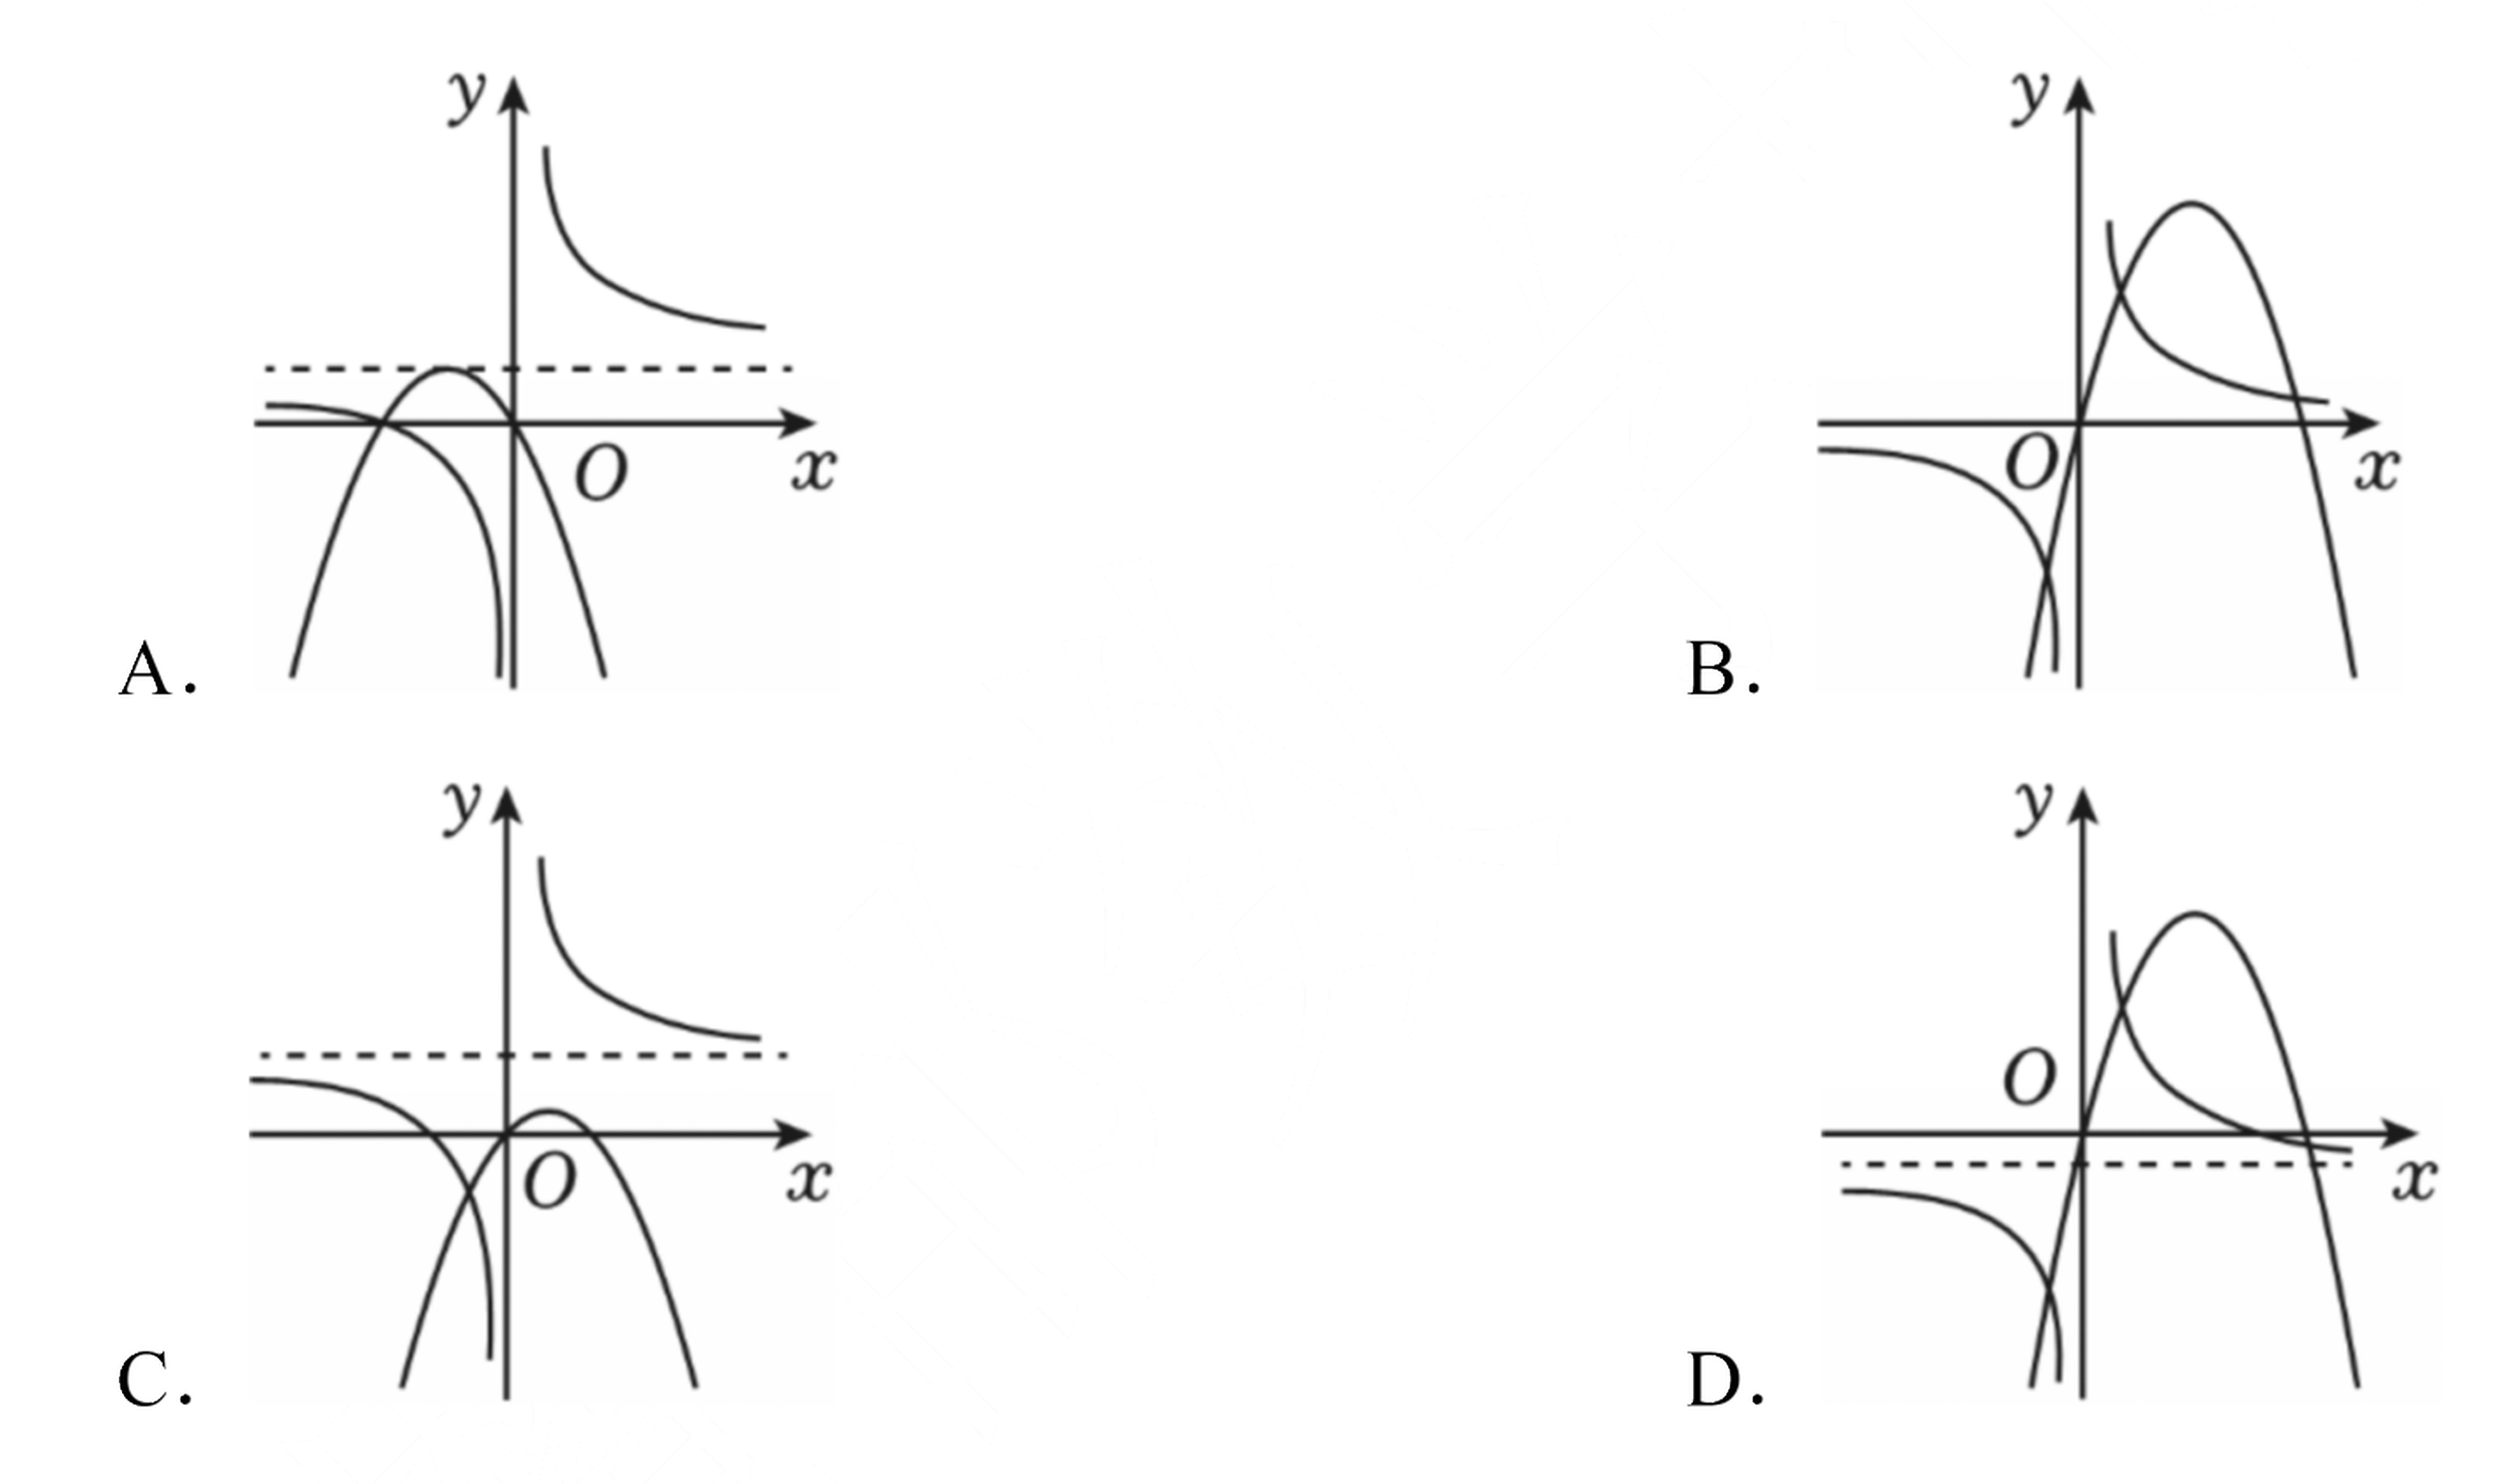
\includegraphics[width=0.80\textwidth]{figures/gao161_q14.png}
\end{center}

\ifanswer
\solbegin
\step{$A$ 选项，由二次函数图象得 $a<0$，$b<0$，由幂函数型函数图象得 $a<0$，$b>0$，}
\step{故 $A$ 选项错误；}
\step{$B$ 选项，由二次函数图象得 $a<0$，$b>0$，由幂函数型函数图象得 $a<0$，$b=0$，}
\step{故 $B$ 选项错误；}
\step{$C$ 选项，由二次函数图象得 $a<0$，$b>0$，由幂函数型函数图象得 $a<0$，$b>0$，}
\step{故 $C$ 选项正确；}
\step{$D$ 选项，由二次函数图象得 $a<0$，$b>0$，由幂函数型函数图象得 $a<0$，$b<0$，}
\step{故 $D$ 选项错误.}
\step{故选 $C$.}
\solend
\fi

% === Q15 === \subseteq／\subset、\varnothing、\mid；"排除 C""排除 B、D"正体字母照录；解析 4 行，故选 $A$
\item 设不等式 $\lvert f(x)\rvert+\lvert g(x)\rvert<a$（常数 $a>0$）的解集是 $M$，设不等式 $\lvert f(x)+g(x)\rvert<a$（常数 $a>0$）的解集是 $N$，则\mbox{（\quad）}

\keepwithprev
A. $M\subseteq N$\qquad B. $N\subseteq M$\qquad C. $M\subset N$\qquad D. $N\subset M$

\ifanswer
\solbegin
\step{$x\in M\Rightarrow\lvert f(x)+g(x)\rvert\leqslant\lvert f(x)\rvert+\lvert g(x)\rvert<a\Rightarrow x\in N$，所以 $M\subseteq N$.}
\step{取 $f(x)=g(x)=0$，则 $M=N$，排除 C.}
\step{取 $f(x)=1$，$g(x)=-1$，$a=1$，则 $M=\varnothing$，$N$ 为全体实数，排除 B、D.}
\step{故选 $A$.}
\solend
\fi

% === Q16 === "人文集"定义证明；cases 无；解析 21 行，故选 $B$
\item 设集合 $I_n=\{1,2,\cdots,n\}$，$n\in\N,n\geqslant1$，集合 $P_n=\left\{\dfrac{m}{\sqrt k}\mid m\in I_n,k\in I_n\right\}$，若 $P_n$ 的子集 $A$ 中任意两个元素之和不是整数的平方，则称 $A$ 为 “人文集”. 那么使 $P_n$ 能分成两个交集为空集的 “人文集” 的并集，且这两个人文集的并集恰为 $P_n$ 时，$n$ 的最大值是\mbox{（\quad）}

\keepwithprev
A. 13\qquad B. 14\qquad C. 15\qquad D. 16

\ifanswer
\solbegin
\step{先证当 $n\geqslant15$ 时，$P_n$ 不能分成两个不相交的人文集的并集.}
\step{假设当 $n\geqslant15$ 时，$P_n$ 可以分成两个不相交的人文集的并集，}
\step{设 $A$ 和 $B$ 为两个不相交的人文集，使 $A\cup B=P_n\supseteq I_n$.}
\step{不妨设 $1\in A$，则由于 $1+3=2^2$，所以 $3\notin A$，即 $3\in B$.}
\step{同理可得，$6\in A$，$10\in B$. 又推出 $15\in A$，}
\step{但 $1+15=4^2$，这与 $A$ 为人文集相矛盾.}
\step{再证 $P_{14}$ 满足要求. 当 $k=1$ 时，$P_{14}=\left\{\dfrac{m}{\sqrt k}\mid m\in I_{14},k\in I_{14}\right\}$，}
\step{可以分成 2 个人文集的并集.}
\step{事实上，只要取 $A_1=\{1,2,4,6,9,11,13\}$，$B_1=\{3,5,7,8,10,12,14\}$，}
\step{则 $A_1$ 和 $B_1$ 都是人文集，且 $A_1\cup B_1=P_{14}$.}
\step{当 $k=4$ 时，集合 $\left\{\dfrac{m}{\sqrt k}\mid m\in I_{14}\right\}$ 中，除整数外，}
\step{剩下的数组成集合 $\left\{\dfrac12,\dfrac32,\dfrac52,\cdots,\dfrac{13}{2}\right\}$，}
\step{可以分为下列 2 个人文集的并：$A_2=\left\{\dfrac12,\dfrac52,\dfrac92,\dfrac{11}{2}\right\}$，$B_2=\left\{\dfrac32,\dfrac72,\dfrac{13}{2}\right\}$.}
\step{当 $k=9$ 时，集合 $\left\{\dfrac{m}{\sqrt k}\mid m\in I_{14}\right\}$ 中，除整数外，}
\step{剩下的数组成集合 $\left\{\dfrac13,\dfrac23,\dfrac43,\dfrac53,\cdots,\dfrac{13}{3},\dfrac{14}{3}\right\}$，}
\step{可以分为下列 2 个人文集的并：$A_3=\left\{\dfrac13,\dfrac43,\dfrac53,\dfrac{10}{3},\dfrac{13}{3}\right\}$，$B_3=\left\{\dfrac23,\dfrac73,\dfrac83,\dfrac{11}{3},\dfrac{14}{3}\right\}$.}
\step{最后，集合 $C=\left\{\dfrac{m}{\sqrt k}\mid m\in I_{14},k\in I_{14},k\ne1,4,9\right\}$ 中的数的分母都是无理数，}
\step{它与 $P_n$ 中的任何其他数之和都不是整数，}
\step{因此，令 $A=A_1\cup A_2\cup A_3\cup C$，$B=B_1\cup B_2\cup B_3$，}
\step{则 $A$ 和 $B$ 是不相交的人文集，且 $A\cup B=P_{14}$.}
\step{综上，$n$ 的最大值为 14，故选 $B$.}
\solend
\fi

\end{enumerate}

\bigsec{三、解答题}

\begin{enumerate}
\setcounter{enumi}{16}

% === Q17 === "图像"照录；\Z；cases 块；解析 9 行，跨 06—07 页
\item (1) 已知函数 $y=x^{\frac{4m-m^2}{2}}$（$m\in\Z$）在区间 $(0,+\infty)$ 上是严格增函数，它的图像关于 $y$ 轴对称，求 $m$ 的值及该函数的解析式；

(2) 若 $(a-2)^{\frac32}<(1+2a)^{\frac32}$，求实数 $a$ 的取值范围.

\ifanswer
\solbegin
\step{(1) 由幂函数在 $(0,+\infty)$ 上严格递增，得 $\dfrac{4m-m^2}{2}>0\Leftrightarrow0<m<4$，}
\step{又 $m\in\Z$，所以 $m\in\{1,2,3\}$.}
\step{当 $m=1$ 或 $m=3$ 时，函数为 $y=x^{\frac32}$，定义域为 $[0,+\infty)$，}
\step{图像不关于 $y$ 轴对称.}
\step{当 $m=2$ 时，函数为 $y=x^2$，满足题意，所以 $m=2$，解析式 $y=x^2$.}
\step{(2) 原不等式有意义，须满足 $\begin{cases}a-2\geqslant0\\1+2a\geqslant0\end{cases}\Leftrightarrow a\geqslant2$，}
\step{函数 $y=x^{\frac32}$ 在 $[0,+\infty)$ 上严格递增，}
\step{因此 $(a-2)^{\frac32}<(1+2a)^{\frac32}\Leftrightarrow a-2<1+2a\Leftrightarrow a>-3$，}
\step{结合 $a\geqslant2$，得 $a\in[2,+\infty)$.}
\solend
\fi

% === Q18 === 题干"$a\geqslant0$"与解析"$a<0$"自相矛盾照录；"$A\cap B=(-2,-1]\cap[2,6)$"误印 ∩ 照录；\subseteq；解析 10 行
\item 已知实数 $a\geqslant0$，集合 $A=\left\{x\mid\dfrac{x+2}{x-6}<0\right\}$，$B=\{x\mid\lvert2x-1\rvert\geqslant3\}$，$C=\{x\mid x^2-3ax+2a^2<0\}$，

(1) 求 $A\cap B$；

(2) 若 $C\subseteq(A\cap B)$，求 $a$ 的取值范围.

\ifanswer
\solbegin
\step{(1) 由 $\dfrac{x+2}{x-6}<0$ 得 $-2<x<6$，即 $A=\{x\mid-2<x<6\}=(-2,6)$，}
\step{由 $\lvert2x-1\rvert\geqslant3$ 得 $2x-1\geqslant3$ 或 $2x-1\leqslant-3$，解得 $x\geqslant2$ 或 $x\leqslant-1$，}
\step{即 $B=(-\infty,-1]\cup[2,+\infty)$，}
\step{所以 $A\cap B=(-2,-1]\cap[2,6)$；}% 原卷把 ∪ 误印成 ∩，照录未改（见 ⑤ 2）
\step{(2) 由 (1) 得 $A\cap B=\{x\mid-2<x\leqslant-1\text{ 或 }2\leqslant x<6\}$，}
\step{因为 $C\subseteq(A\cap B)$，$x^2-3ax+2a^2=(x-a)(x-2a)<0$，}% 题干 $a\geqslant0$ 与解析 $a<0$ 自相矛盾，照录未改（见 ⑤ 1）
\step{当 $a=0$ 时，$C=\varnothing$，符合题意；}
\step{当 $a>0$ 时，$C=(a,2a)$，则 $\begin{cases}a\geqslant2\\2a\leqslant6\\a>0\end{cases}$，解得 $2\leqslant a\leqslant3$，}
\step{当 $a<0$ 时，$C=(2a,a)$，则 $\begin{cases}2a\geqslant-2\\a\leqslant-1\\a<0\end{cases}$，解得 $a=-1$，}
\step{故 $a$ 的范围为 $\{-1,0\}\cup[2,3]$.}
\solend
\fi

% === Q19 === 双碳太阳能应用题；"双碳""自发自用、市电互补"弯引号；解析 8 行，跨 08 页上下
\item 为响应 “双碳” 目标，某电子企业拟安装一套可使用 10 年的太阳能供电设备. 该设备的安装费用 $P(x)$（单位：万元）与太阳能电池板面积 $x(x>0)$（单位：平方米）成正比，比例系数为 $\dfrac12$. 为保障生产用电，安装后采用 “自发自用、市电互补” 模式，在此模式下，企业每年消耗的电费 $Q(x)$（单位：万元）与安装的这种太阳能电池板的面积 $x$ 之间的函数关系是 $Q(x)=\dfrac{180}{x+5}$. 记 $W(x)$（单位：万元）为该企业安装这种太阳能供电设备的费用与 10 年所消耗的电费之和.

(1) 要使该设备的安装费与第 1 年的电费之和不超过 17 万元，求安装太阳能电池板面积 $x$ 的取值范围；

(2) 当 $x$ 为多少平方米时，$W(x)$ 取得最小值？最小值是多少万元？

\ifanswer
\solbegin
\step{(1) $P(x)=\dfrac{x}{2}$，安装费与第 1 年的电费之和不超过 17 万元，即 $\dfrac{x}{2}+\dfrac{180}{x+5}\leqslant17$，}
\step{$x>0$，上式等价于 $x^2-29x+190\leqslant0\Leftrightarrow(x-10)(x-19)\leqslant0$，}
\step{解得 $x\in[10,19]$.}
\step{(2) 安装费用与 10 年电费之和为 $W(x)=P(x)+10Q(x)$，}
\step{$=\dfrac{x}{2}+\dfrac{1800}{x+5}=\dfrac{x+5}{2}+\dfrac{1800}{x+5}-\dfrac52$，}
\step{$x>0$，由基本不等式得 $W(x)\geqslant2\sqrt{\dfrac{x+5}{2}\cdot\dfrac{1800}{x+5}}-\dfrac52=60-\dfrac52=57.5$，}
\step{等号当且仅当 $\dfrac{x+5}{2}=\dfrac{1800}{x+5}$，即 $x=55$ 时成立.}
\step{因此，当电池板面积为 55 平方米时，$W(x)$ 取得最小值 57.5 万元.}
\solend
\fi

% === Q20 === $a*b$ 定义；\min 改正体；cases 块；解析 23 行，跨 08—10 页
\item 设 $a$、$b\in\R$，定义 $a*b=\begin{cases}a,&a<b\\b,&a\geqslant b\end{cases}$.

(1) 若 $x*2>1$，求 $x$ 的取值范围；

(2) 若 $(\lvert x-1\rvert+\lvert x-2\rvert)*3=3$，求 $x$ 的取值范围；

(3) 若 $a$、$b>0$，记 $M=a*\dfrac{b}{a^2+4b^2}$，分别比较 $M$ 与 $a$，以及 $M$ 与 $\dfrac{b}{a^2+4b^2}$ 的大小，并求 $M$ 的最大值.

\ifanswer
\solbegin
\step{(1) 定义 $a*b=\begin{cases}a,&a<b\\b,&a\geqslant b\end{cases}$，由 $x*2>1$，得 $\begin{cases}x<2\\x>1\end{cases}$，或 $\begin{cases}x\geqslant2\\2>1\end{cases}$，}
\step{解得 $x>1$，即 $x$ 的取值范围为 $\{x\mid x>1\}$；}
\step{(2) 当 $x\geqslant2$ 时，$\lvert x-1\rvert+\lvert x-2\rvert=2x-3\geqslant1$，}
\step{当 $1\leqslant2x-3\leqslant3$，即 $2\leqslant x\leqslant3$ 时，}
\step{此时 $(\lvert x-1\rvert+\lvert x-2\rvert)*3=2x-3=3$，解得 $x=3$；}
\step{当 $2x-3>3$，即 $x>3$ 时，}
\step{此时 $(\lvert x-1\rvert+\lvert x-2\rvert)*3=3$ 恒成立，则 $x>3$；}
\step{当 $-2x+3>3$，即 $x<0$ 时，}
\step{此时 $(\lvert x-1\rvert+\lvert x-2\rvert)*3=3$ 恒成立，则 $x<0$.}
\step{当 $1<x<2$ 时，$\lvert x-1\rvert+\lvert x-2\rvert=1$，}
\step{此时 $(\lvert x-1\rvert+\lvert x-2\rvert)*3=1\ne3$，不符合题意；}
\step{当 $x\leqslant1$ 时，$\lvert x-1\rvert+\lvert x-2\rvert=-2x+3\geqslant1$，}
\step{当 $-2x+3\leqslant3$，即 $0\leqslant x\leqslant1$ 时，}
\step{此时 $(\lvert x-1\rvert+\lvert x-2\rvert)*3=-2x+3=3$，解得 $x=0$.}
\step{综上所述，$x$ 的取值范围为 $\{x\mid x\leqslant0\text{ 或 }x\geqslant3\}$；}
\step{(3) 由题意，$M=a*\dfrac{b}{a^2+4b^2}=\min\left\{a,\dfrac{b}{a^2+4b^2}\right\}$，}% 原卷印斜体 min，按全稿惯例改正体 \min（见 ② ⑬）
\step{则 $M\leqslant a$，$M\leqslant\dfrac{b}{a^2+4b^2}$.}
\step{因为 $a$、$b>0$，所以 $\dfrac{b}{a^2+4b^2}\leqslant\dfrac{b}{2\sqrt{a^2\cdot4b^2}}=\dfrac{1}{4a}$，}
\step{当且仅当 $a=2b>0$ 时取等号，}
\step{当 $a\geqslant\dfrac{1}{4a}$，即 $a\geqslant\dfrac12$ 时，$M=a*\dfrac{b}{a^2+4b^2}=\dfrac{b}{a^2+4b^2}\leqslant\dfrac{1}{4a}$，}
\step{则 $a=\dfrac12$，$b=\dfrac14$ 时，$M$ 取得最大值 $\dfrac12$；}
\step{当 $0<a<\dfrac12$ 时，$M=a*\dfrac{b}{a^2+4b^2}=a$，此时 $M<\dfrac12$.}
\step{综上所述，$M$ 的最大值为 $\dfrac12$.}
\solend
\fi

% === Q21 === $A_n$／$B_n$／$S_n$／$T_n$ 新定义；题干第 3 问误标 (2) 照录、解析作 (3)；\prec；解析 25 行，跨 10—11 页
\item 对任意正整数 $n$，记集合 $A_n=\{(a_1,a_2,\cdots,a_n)\mid a_1,a_2,\cdots,a_n$ 均为非负整数，且 $a_1+a_2+\cdots+a_n=n\}$，集合 $B_n=\{(b_1,b_2,\cdots,b_n)\mid b_1,b_2,\cdots,b_n$ 均为非负整数，且 $b_1+b_2+\cdots+b_n=2n\}$. 设 $\alpha=(a_1,a_2,\cdots,a_n)\in A_n$，$\beta=(b_1,b_2,\cdots,b_n)\in B_n$，若对任意 $i\in\{1,2,\cdots,n\}$ 都有 $a_i\leqslant b_i$，则记 $\alpha\prec\beta$.

(1) 写出集合 $A_2$ 和 $B_2$；

(2) 证明：对任意 $\alpha\in A_n$，存在 $\beta\in B_n$，使得 $\alpha\prec\beta$；

(2) 设集合 $S_n=\{(\alpha,\beta)\mid\alpha\in A_n,\beta\in B_n,\alpha\prec\beta\}$，求证：$S_n$ 中的元素个数是完全平方数.% 原卷第 3 问题干误标 (2)（与第 2 问重号），照录未改（见 ⑤ 3）

\ifanswer
\solbegin
\step{(1) $A_2=\{(0,2),(1,1),(2,0)\}$，$B_2=\{(0,4),(1,3),(2,2),(3,1),(4,0)\}$；}
\step{(2) 对任意 $\alpha=(a_1,a_2,\cdots,a_n)\in A_n$，设 $b_i=a_i+1$（$i=1,2,3,\cdots,n$），}
\step{则 $b_1,b_2,\cdots,b_n$ 均为非负整数，且 $a_i\leqslant b_i$（$i=1,2,3,\cdots,n$）.}
\step{令 $\beta=(b_1,b_2,\cdots,b_n)$，则 $b_1+b_2+\cdots+b_n$}
\step{$=(a_1+1)+(a_2+1)+\cdots+(a_n+1)=(a_1+a_2+\cdots+a_n)+n=2n$，}
\step{所以 $\beta\in B_n$，且 $\alpha\prec\beta$.}
\step{(3) 对任意 $\alpha=(a_1,a_2,\cdots,a_n)\in A_n$，$\alpha'=(a_1',a_2',\cdots,a_n')\in A_n$，}
\step{记 $\alpha+\alpha'=(a_1+a_1',a_2+a_2',\cdots,a_n+a_n')$，}
\step{则 $a_1+a_1',a_2+a_2',\cdots,a_n+a_n'$ 均为非负整数，}
\step{且 $(a_1+a_1')+(a_2+a_2')+\cdots+(a_n+a_n')$}
\step{$=(a_1+a_2+\cdots+a_n)+(a_1'+a_2'+\cdots+a_n')=n+n=2n$，}
\step{所以 $\alpha+\alpha'\in B_n$，且 $\alpha\prec\alpha+\alpha'$，$\alpha'\prec\alpha+\alpha'$.}
\step{设集合 $A_n$ 中的元素个数为 $t$，设 $A_n=\{\alpha_1,\alpha_2,\cdots,\alpha_t\}$.}
\step{设集合 $T_n=\{(\alpha_i,\alpha_i+\alpha_j)\mid i=1,2,\cdots,t,j=1,2,\cdots,t\}$.}
\step{对任意 $\alpha_i\in A_n$（$i=1,2,\cdots,t$），都有 $\alpha_i+\alpha_1,\alpha_i+\alpha_2,\cdots,\alpha_i+\alpha_t\in B_n$，}
\step{且 $\alpha_i\prec\alpha_i+\alpha_j$，$j=1,2,\cdots,t$，所以 $T_n\subseteq S_n$.}
\step{若 $(\alpha,\beta)\in S_n$，其中 $\alpha=(a_1,a_2,\cdots,a_n)\in A_n$，$\beta=(b_1,b_2,\cdots,b_n)\in B_n$，}
\step{设 $c_i=b_i-a_i$（$i=1,2,\cdots,n$），因为 $a_i\leqslant b_i$，所以 $c_i=b_i-a_i\geqslant0$，}
\step{记 $\alpha'=(c_1,c_2,\cdots,c_n)$，}
\step{则 $c_1+c_2+\cdots+c_n=(b_1-a_1)+(b_2-a_2)+\cdots+(b_n-a_n)$}
\step{$=(b_1+b_2+\cdots+b_n)-(a_1+a_2+\cdots+a_n)=2n-n=n$，}
\step{所以 $\alpha'\in A_n$，并且有 $\beta=\alpha+\alpha'$，所以 $(\alpha,\beta)\in T_n$，所以 $S_n\subseteq T_n$，}
\step{所以 $S_n=T_n$.}
\step{因为集合 $T_n$ 中的元素个数为 $t^2$，所以 $S_n$ 中的元素个数为 $t^2$，}
\step{是完全平方数.}
\solend
\fi

\end{enumerate}

\end{document}
"
%
% ① 原始材料：微信公众号"魔都数学加油站"文章，连载"27学年高一161"，原卷卷面标题
% "2026-2027 年松江一中嘉一实验高一上期中"（卷面未印副标题、未印连载号）。
% 正文为 11 张 PNG 页（01/02/03/05/06/07/08/09/11 为 4762×6735，04/10 为
% 2560×3620，同一篇各页分辨率混排，逐页按各自分辨率裁图核对）。
% 体例：讲评版——填空 3—12（10 题）、选择 13—16（4 题）、解答 17—21（5 题），
% 共 19 题，自第 3 题起编（1、2 未印在本篇）；Q13 答案"A"直接印在题干括号内、
% 且无【答案】/【解析】段，本稿按 高一37 第 13 题／高一57 第 13 题成例把括号
% 留空、另提 \ans{$A$}；其余 18 题逐题印【解析】、用 \solbegin…\solend。
% 题目、答案、解析均据原图转录；卷面粉红色水印"魔都数学加油站"及公众号页脚未录入。
% 全卷插图清单（逐页通读 11 页确认）：仅 1 组——Q14 四幅图像选项（04 页 2×2
% 排布，二次函数与幂函数型函数在同一坐标系中的图象，A/B/C/D 四幅小图），
% 合并成一张，三版都出，裁 figures/gao161_q14.png。其余各页逐页确认无其它
% 题目配图、无解析内配图、无表格、无"如图"处（Q16 解析里的"可以分为下列 2 个
% 人文集的并"是纯文字＋集合，不是表格；OCR 里看似表格的行实为大括号与分数）。
%
% 卷首标题：原卷印作"2026-2027 年松江一中嘉一实验高一上期中"，年份区间按全稿惯例排 en dash；
% 原卷卷面未印副标题，本稿按同期中卷知识模块口径补出"集合与常用逻辑用语、不等式、函数"。
%
% ② 与原卷的排版差异／照录项清单：
%   ① 原文从第 3 题起，本稿保留原题号；共 19 题三节，解答题 5 题到 21；
%      三节各自一个 enumerate + \setcounter{enumi}{2}/{12}/{16}（不贯穿），
%      用 \examtitlest[3] 起手；
%   ② 混合体例：Q13 原卷把答案"A"直接印在题干括号内（"（  A  ）"）、且题下
%      无【答案】/【解析】段，按 高一37 第 13 题／高一57 第 13 题成例把括号
%      留空、另提 \ans{$A$}、不补造解析；其余 18 题印【解析】、用
%      \solbegin…\solend；四道选择题中 Q14/Q15/Q16 的答案在解析末句
%      "故选 $C$／$A$／$B$"、Q13 用 \ans{$A$}；括号 \mbox{（\quad）} 留空；
%      答案版【答案】/【解析】标记数 = 19 = 全卷题数（1 个 \ans ＋ 18 个 \solbegin）；
%   ③ 原卷卷面未印副标题，本稿按知识模块口径补出；
%   ④ 原卷填空横线按全稿惯例排 \blankline[4.4em]；选择题选项段前按惯例各加
%      \keepwithprev；Q14 四幅选项图整块用 \needvspace{9cm} 守卫（守卫放
%      \item 之前，见 高一132 Q14／高一154 Q15 成例）；解答题不留作答区、
%      不加 \anspace（原卷为讲评版）；
%   ⑤ 数集归一：Q8"$x\in\R$"、Q11"$m\in\R$"、Q13"$x,y\in\N$"、
%      Q16"$n\in N$"、Q17"$m\in\Z$"、Q20"$a$、$b\in R$"——原卷印正体粗体
%      或斜体 R/N/Z，按全稿惯例归一 \R／\N／\Z；绝对值排 \lvert…\rvert
%      （Q9、Q12、Q15、Q18、Q20），集合描述竖线排 \mid（Q12、Q16、Q18、
%      Q20、Q21），空集 \varnothing（Q15、Q18），补集无用例，不等号按全稿
%      惯例排 \leqslant／\geqslant；
%   ⑥ 子集符号逐处照录不统一：Q12 cases 定义"$C(A)\geqslant C(B)$"、
%      Q15 选项 A/B"$M\subseteq N$""$N\subseteq M$"与解析"$M\subseteq N$"
%      印带下划线 ⊆（照录 \subseteq），Q15 选项 C/D"$M\subset N$""$N\subset M$"
%      印单线 ⊂（照录 \subset），Q18 "$C\subseteq(A\cap B)$"、Q21
%      "$T_n\subseteq S_n$""$S_n\subseteq T_n$"均带下划线照录 \subseteq；
%      本卷无 \not\subset 用例；
%   ⑦ 判别式：Q7 解析"$\Delta=(m-6)(m+2)>0$"、Q8 解析"$\Delta=a^2-4a<0$"、
%      Q12 解析"$\Delta=a^2-8$"共 3 处，逐处放大确认印等腰偏高粗三角
%      （高>宽、右斜边粗），照录 \Delta；本卷无扁等边细线 \triangle 用例；
%   ⑧ 中文弯引号照录：Q7"$m\geqslant6$""有两个不相等的正实数根"及四个
%      条件短语、Q13 反证法命题、Q16"人文集"、Q19"双碳""自发自用、市电互补"；
%      注释里一律 ASCII 引号；数学式内 CJK 用 \text{}（Q18、Q20 解集描述内"或"）；
%   ⑨ "图像／图象"逐处照录不统一：Q4"的图像"、Q17 题干"它的图像关于 $y$ 轴
%      对称"及解析"图像不关于 $y$ 轴对称"印"图像"；Q14 题干"的图象可能为"
%      与解析 A/B/C/D 四行各"由二次函数图象得""由幂函数型函数图象得"
%      共 8 处印"图象"（象，无亻）；
%   ⑩ 文本圈数字逐处照录：Q12 题干①②③④、Q12 解析"故①错误""故②正确"
%      "故③正确""故④错误""故正确的是②③"，均为印刷圈数字（文本模式）；
%   ⑪ 半角逗号在数学组之间是全稿惯例、非笔误，逐处照录（Q5"$a$、$b$"、
%      Q13"$x,y\in\N$"、Q16"$n\in\N,n\geqslant1$"与集合描述内逗号、
%      Q20"$a,b\in\R$"、Q21 各集合描述内逗号）；行末西文句点 ASCII `.`；
%      原卷行中句点（Q16"$10\in B$. 又推出 $15\in A$"、Q16"再证 $P_{14}$
%      满足要求. 当 $k=1$ 时"、Q18"$A\cap B=(-2,-1]\cap[2,6)$；"后的分号）
%      按全稿惯例一律排 ASCII `.`／全角"；"；中文语境行中全角逗号／顿号照录；
%   ⑫ 原卷数学式内联条件（Q14"$y=x^a+b(a\ne0)$"、Q19"$x(x>0)$"、
%      Q11"$\lvert x-m\rvert<n\,(m\in\R,n>0)$"）印半角括号，逐处照录未改
%      全角（同 高一147 口径）；
%      中文语境的括注（Q5"结果用 $a$、$b$ 表示"、Q7"填…"、Q12"填写序号"、
%      Q15"常数 $a>0$"、Q19"单位：万元"）印全角括号，照录；
%   ⑬ 复杂式照录别简化：Q3 $(a^{2-\sqrt3})^{2+\sqrt3}\times\sqrt{a^2}\times
%      b^{\sqrt3}\times b^{1-\sqrt3}$ 与 $a^{(2-\sqrt3)(2+\sqrt3)}\cdot a\cdot
%      b^{\sqrt3+1-\sqrt3}=a\cdot a\cdot b=a^2b$（题干用 \times、解析用 \cdot，
%      逐处照录不统一，见 ⑤）；Q5 $\dfrac{\lg2}{\lg2+\lg3}=\dfrac{a}{a+b}$、
%      Q10 $t-\dfrac3t=2$ 与 $b=a^3$、$ab=a^4=2$、Q11 $\left(2a-\dfrac12
%      -a+\dfrac12,2a-\dfrac12+a-\dfrac12\right)=(a,3a-1)$ 与
%      $\left(\dfrac43,\dfrac53\right]\cup\{2\}$、Q16 各分数集合、Q19
%      $x^2-29x+190\leqslant0$ 与 $W(x)=P(x)+10Q(x)$ 与
%      $2\sqrt{\dfrac{x+5}{2}\cdot\dfrac{1800}{x+5}}-\dfrac52=60-\dfrac52=57.5$、
%      Q20 $M=a*\dfrac{b}{a^2+4b^2}=\min\left\{a,\dfrac{b}{a^2+4b^2}\right\}$
%      与 $\dfrac{b}{2\sqrt{a^2\cdot4b^2}}=\dfrac{1}{4a}$、Q21 各 $A_n$／$B_n$／
%      $T_n$ 定义；\left…\right 不得拆到不同 $…$ 组（Q11 的 \left(…\right)、
%      Q11 的 \left(\dfrac43,\dfrac53\right]、Q16 的 \left\{\dfrac{m}{\sqrt k}
%      \mid…\right\} 与 \left\{\dfrac12,\dfrac32,\dfrac52,\cdots,\dfrac{13}{2}\right\}
%      等、Q20 的 \min\left\{…\right\}）；cases 块整体算一个印刷行
%      （Q12 定义、Q17 (2)、Q18 (2) 两处、Q20 定义与 (1)）；原卷 Q20 解析
%      "$=min\{…\}$"印斜体 min，按 高一122／高一102 成例改正体 \min；
%   ⑭ 一条 \step = 原卷解析的一个印刷行；别并折行、别拆行。跨页续印按题合并
%      （Q6 的 01 页上下题干重复印、Q10 的 01—02 页、Q11 的 02—03 页、
%      Q12 的 03—04 页、Q16 的 05—06 页、Q17 的 06—07 页、Q18 的 07 页
%      上下、Q19 的 08 页上下、Q20 的 08—10 页、Q21 的 10—11 页）；
%      跨半页重叠行（Q10"令 $t=\log_a b>0$…"、Q16"它与 $P_n$ 中的任何
%      其他数之和都不是整数，"、Q18"【解析】(1) 由 $\dfrac{x+2}{x-6}<0$…"、
%      Q19"$x>0$，上式等价于…"、Q20"此时…则 $x<0$."、Q21"若 $(\alpha,\beta)
%      \in S_n$…"与"设 $c_i=b_i-a_i$…"）只算一个印刷行；
%   ⑮ 自定义记号照录：Q12"$C(A)$""$A*B$""$S$"、Q16"$I_n$""$P_n$""人文集"
%      "$A_1$／$B_1$／$A_2$／$B_2$／$A_3$／$B_3$／$C$"、Q20"$a*b$""$M$"、
%      Q21"$A_n$／$B_n$／$S_n$／$T_n$""$\alpha\prec\beta$""$\alpha+\alpha'$"；
%   ⑯ 选项字母体例照录不统一：Q15 解析"排除 C.""排除 B、D."两处原卷印
%      正体（文本模式），Q13 \ans{$A$}、Q14"$A$ 选项"…"故选 $C$"、
%      Q15"故选 $A$"、Q16"故选 $B$"用斜体（数学模式），逐处照录、不统一；
%   ⑰ 红字：全卷逐页扫描无红色加粗小标题（仅粉色水印），故本卷无 \stepm，
%      不引入红色定义；
%
% ③ 行数复核：一条 \step = 原卷解析的一个印刷行，cases 块作一个印刷行计。
%   逐题数（逐页核对定稿）：Q3：1；Q4：1；Q5：1；Q6：3；Q7：4；Q8：4；
%   Q9：2；Q10：2；Q11：7；Q12：8；Q13：0（答案印括号内、提 \ans{}，
%   不计入 \step 账）；Q14：9；Q15：4；Q16：21；Q17：9；Q18：10；Q19：8；
%   Q20：23；Q21：25。
%   合计 142 行（142 条 \step，无 \stepm），与原卷逐题印刷行相等。
%   全卷 19 题：Q13 一处 \ans{} ＋ 其余 18 题设 \solbegin…\solend，
%   答案版【答案】/【解析】标记数 = 19 = 全卷题数。
%
% ④ 页码分布（供回原图复核）：
%   卷首标题＋"一、填空题"＋Q3/Q4/Q5 题干＋解析各 1 行＋Q6 题干首行
%   在 01 页上半；Q6 题干（重复印）＋解析 3 行＋Q7 题干＋解析 4 行在
%   01 页下半；Q8 题干＋解析 4 行＋Q9 题干＋解析 2 行＋Q10 题干＋
%   解析首行在 02 页上半；Q10 解析（重复印）＋末行＋Q11 题干＋解析
%   前 3 行在 02 页下半；Q11 解析后 4 行＋Q12 题干＋cases 定义＋①
%   在 03 页上半；Q12 ②③④ 三命题＋"填写序号"行＋解析前 6 行在
%   03 页下半；Q12 解析后 2 行＋"二、选择题"标题＋Q13 题干＋选项＋
%   Q14 题干＋"（　）"＋A/B 两幅图在 04 页上半；Q14 四幅图（重复印）
%   ＋解析 9 行在 04 页下半；Q15 题干＋选项＋解析 4 行＋Q16 题干＋
%   选项在 05 页上半；Q16 题干（重复印）＋选项＋解析前 10 行在 05 页
%   下半；Q16 解析中 8 行（k=4、k=9 两批＋集合 C＋"它与 $P_n$…"）
%   在 06 页上半；Q16 解析"它与 $P_n$…"（重复印）＋末 3 行＋
%   "三、解答题"标题＋Q17 题干＋两问＋解析前 4 行在 06 页下半；
%   Q17 解析后 5 行＋Q18 题干＋两问＋解析首行在 07 页上半；Q18 解析
%   （重复首行）＋余 9 行在 07 页下半；Q19 题干＋两问＋解析前 2 行在
%   08 页上半；Q19 解析（重复第 2 行）＋余 6 行＋Q20 定义＋(1) 问在
%   08 页下半；Q20 (2)(3) 两问＋解析 (1) 2 行＋(2) 前 7 行在 09 页
%   上半；Q20 解析 (2) 余 4 行＋(3) 前 4 行在 09 页下半；Q20 解析 (3)
%   余 4 行＋Q21 题干＋三问在 10 页上半；Q21 题干（重复印）＋解析
%   (1)(2)(3) 前 8 行在 10 页下半；Q21 解析 (3) 中 10 行在 11 页上半；
%   Q21 解析 (3)（重复 2 行）＋末 7 行"是完全平方数."在 11 页下半。
%   本稿按题连排，不丢行、不并折行；全卷末题为第 21 题，无附加题节。
%
% ⑤ 存疑照录（放大原图确认，照录未改、正文对应处另有 % 注）：
%   1. Q18 题干印"已知实数 $a\geqslant0$"，解析却另设"当 $a<0$ 时"并解出
%      $a=-1$，末行答案"故 $a$ 的范围为 $\{-1,0\}\cup[2,3]$"含负数，
%      与题干 $a\geqslant0$ 自相矛盾——系原卷前后不一，照录未改（放大
%      07 页确认题干确印 $a\geqslant0$）；
%   2. Q18 解析"所以 $A\cap B=(-2,-1]\cap[2,6)$；"原卷把并集误印成
%      交集号 ∩（紧接下一行"$A\cap B=\{x\mid-2<x\leqslant-1$ 或
%      $2\leqslant x<6\}$"用"或"），照录未改（放大 07 页确认印 ∩）；
%   3. Q21 题干第 3 问原卷标号印作"(2)"（与第 2 问重号），而解析里
%      同一问标作"(3)"——原卷笔误，题干与解析逐处照录、不统一；
%   4. Q3 题干四处乘号印"×"（\times）、解析内三处乘号印"·"（\cdot），
%      逐处照录未统一（放大 01 页确认）；
%   5. Q16 解析"先证当 $n\geqslant15$ 时"印 ≥（非 >），与"综上，$n$
%      的最大值为 14"自洽，照录；题干"$n\in N,n\geqslant1$"印斜体
%      $N$、按全稿惯例归一 \N（见 ② ⑤）；
%   6. Q20 解析"$M=a*\dfrac{b}{a^2+4b^2}=min\{…\}$"原卷印斜体 min，
%      按全稿惯例改正体 \min（见 ② ⑬）；末行"$M$ 的最大值为
%      $\dfrac12$"照录；
%   7. Q15 解析"排除 C.""排除 B、D."用正体字母，而"故选 $A$"用斜体
%      字母，原卷体例不一（见 ② ⑯），照录未统一。
%   全卷除此 7 类外未发现其它笔误／自相矛盾处；Q13 只把答案印在括号内、
%   其余 18 题全部印【解析】。
%

\documentclass[a4paper,11pt]{article}
\usepackage{common}

\begin{document}

\examtitlest[3]{2026--2027 年松江一中嘉一实验高一上期中}{集合与常用逻辑用语、不等式、函数}

\bigsec{一、填空题}

\begin{enumerate}
\setcounter{enumi}{2}

% === Q3 === 题干 \times、解析 \cdot 逐处照录；解析 1 行
\item 设 $a>0$，$b>0$，化简 $(a^{2-\sqrt3})^{2+\sqrt3}\times\sqrt{a^2}\times b^{\sqrt3}\times b^{1-\sqrt3}=$\blankline[4.4em].

\ifanswer
\solbegin
\step{因为 $a>0$，所以 $\sqrt{a^2}=a$，原式 $=a^{(2-\sqrt3)(2+\sqrt3)}\cdot a\cdot b^{\sqrt3+1-\sqrt3}=a\cdot a\cdot b=a^2b$.}
\solend
\fi

% === Q4 === "图像"照录；解析 1 行
\item 若幂函数 $y=x^a$ 的图像经过点 $(5,\sqrt5)$，则此幂函数的表达式为 $y=$\blankline[4.4em].

\ifanswer
\solbegin
\step{$5^a=\sqrt5\Rightarrow a=\dfrac12$，所以 $y=\sqrt x$.}
\solend
\fi

% === Q5 === "结果用 $a$、$b$ 表示"全角括号＋顿号照录；解析 1 行
\item 已知 $\lg2=a$，$10^b=3$，则 $\log_6 2=$\blankline[4.4em]（结果用 $a$、$b$ 表示）.

\ifanswer
\solbegin
\step{$\lg3=b$，$\log_6 2=\dfrac{\lg2}{\lg2+\lg3}=\dfrac{a}{a+b}$.}
\solend
\fi

% === Q6 === 对称中心；解析 3 行，题干跨 01 页上下重复印
\item 若函数 $y=\dfrac{mx-1}{x+n}$ 的对称中心是 $(4,-3)$，则 $m+n=$\blankline[4.4em].

\ifanswer
\solbegin
\step{令 $x=-n+t$（$t\ne0$），则 $y-m=-\dfrac{mn+1}{t}$；}
\step{将 $t$ 换成 $-t$，$y-m$ 变为其相反数，因此对称中心为 $(-n,m)$.}
\step{于是 $n=-4$，$m=-3$，得 $m+n=-7$.}
\solend
\fi

% === Q7 === 充要条件；中文弯引号＋圈选条件；\Delta 高瘦；解析 4 行
\item 已知关于 $x$ 的一元二次方程 $x^2-mx+m+3=0$，则 “$m\geqslant6$” 是该方程 “有两个不相等的正实数根” 的\blankline[4.4em]条件（填 “充分不必要”、“必要不充分”、“充要” 或 “既不充分也不必要”）.

\ifanswer
\solbegin
\step{方程有两个不相等的正实数根}
\step{$\Leftrightarrow m>0$、$m+3>0$ 且 $\Delta=(m-6)(m+2)>0\Leftrightarrow m>6$.}
\step{$m>6\Rightarrow m\geqslant6$，但 $m=6$ 时方程有两个相等的正实数根，}
\step{因此为必要不充分条件.}
\solend
\fi

% === Q8 === \R、\Delta；解析 4 行
\item 对于任意的 $x\in\R$，代数式 $\lg(ax^2+ax+1)$ 都有意义，则实数 $a$ 的取值范围是\blankline[4.4em].

\ifanswer
\solbegin
\step{真数须满足 $ax^2+ax+1>0$ 对任意 $x\in\R$ 恒成立.}
\step{$a=0$ 时成立；}
\step{$a\ne0$ 时，恒成立等价于 $a>0$ 且 $\Delta=a^2-4a<0$，解得 $0<a<4$；}
\step{因此 $a\in[0,4)$.}
\solend
\fi

% === Q9 === 绝对值 \lvert…\rvert；解析 2 行
\item 若不等式 $\lvert x+1\rvert-\lvert x-4\rvert<m$ 的解集为非空集合，则实数 $m$ 的取值范围是\blankline[4.4em].

\ifanswer
\solbegin
\step{$\lvert x+1\rvert-\lvert x-4\rvert\geqslant-\lvert(x+1)-(x-4)\rvert=-5$，当 $x=-1$ 时取等号，}
\step{因此原不等式的解集非空 $\Leftrightarrow m>-5$，所求范围为 $(-5,+\infty)$.}
\solend
\fi

% === Q10 === 换底；$\log_2 a\cdot\log_2 b$；解析 2 行，跨 02 页上下
\item 已知 $a>1$，$b>1$，若 $\log_a b-3\log_b a=2$，且 $ab=2$，则 $\log_2 a\cdot\log_2 b=$\blankline[4.4em].

\ifanswer
\solbegin
\step{令 $t=\log_a b>0$，则 $t-\dfrac{3}{t}=2\Leftrightarrow(t-3)(t+1)=0$，得 $t=3$，}
\step{于是 $b=a^3$，$ab=a^4=2$，得 $\log_2 a=\dfrac14$，$\log_2 b=\dfrac34$，所求为 $\dfrac{3}{16}$.}
\solend
\fi

% === Q11 === 邻域定义；\left(…\right) 不拆组；解析 7 行，跨 02—03 页
\item 对于实数 $m$ 和正数 $n$，称满足不等式 $\lvert x-m\rvert<n\,(m\in\R,n>0)$ 的实数 $x$ 的集合叫做 $m$ 的 $n$ 邻域. 已知 $a>\dfrac12$，若 $2a-\dfrac12$ 的 $a-\dfrac12$ 邻域中恰有 2 个整数，则 $a$ 的取值范围是\blankline[4.4em].

\ifanswer
\solbegin
\step{所求邻域为 $\left(2a-\dfrac12-a+\dfrac12,2a-\dfrac12+a-\dfrac12\right)=(a,3a-1)$.}
\step{当 $\dfrac12<a\leqslant1$ 时至多含 1 个整数；}
\step{当 $a>2$ 时，区间长度 $2a-1>3$，至少含 3 个整数.}
\step{当 $1<a<2$ 时，区间必含 2，恰有两个整数等价于 $3<3a-1\leqslant4$，}
\step{即 $\dfrac43<a\leqslant\dfrac53$.}
\step{当 $a=2$ 时，区间为 $(2,5)$，恰含整数 $3,4$；}
\step{所以 $a\in\left(\dfrac43,\dfrac53\right]\cup\{2\}$.}
\solend
\fi

% === Q12 === $C(A)$／$A*B$ 定义题；①②③④ 文本圈数字；\subseteq／\subset、\Delta、\mid、\varnothing；解析 8 行
\item 用 $C(A)$ 表示非空集合 $A$ 中的元素个数. 对于集合 $A$、$B$，定义

$A*B=\begin{cases}C(A)-C(B),&C(A)\geqslant C(B)\\ C(B)-C(A),&C(A)<C(B)\end{cases}$，若 $A=\{0,1\}$，$B=\{x\mid(x^2-ax)(x^2+ax+2)=0\}$，设实数 $a$ 的所有可能取值组成的集合是 $S$，则下列说法正确的是\blankline[4.4em]（填写序号）.

① $C(B)$ 的可能值为 $2,3,4$

② 若 $A*B=2$，则 $a$ 的取值范围为 $(-\infty,-2\sqrt2)\cup(2\sqrt2,+\infty)$

③ 若 $A*B=1$，则 $C(S)=3$

④ 若 $A*B=0$，则 $a$ 的取值范围为 $(-2\sqrt2,2\sqrt2)$

\ifanswer
\solbegin
\step{$x(x-a)=0$ 的根为 $0,a$，而 $x^2+ax+2$ 在这两处的值分别为 $2,2a^2+2$，}
\step{两个因式无公共实根；后者的判别式为 $\Delta=a^2-8$.}
\step{当 $a=0$、$0<\lvert a\rvert<2\sqrt2$、$\lvert a\rvert=2\sqrt2$、$\lvert a\rvert>2\sqrt2$ 时，$C(B)$ 依次为 $1,2,3,4$，}
\step{故①错误.}
\step{$A*B=\lvert2-C(B)\rvert$，所以 $A*B=2\Leftrightarrow\lvert a\rvert>2\sqrt2$，故②正确；}
\step{$A*B=1\Leftrightarrow a\in\{-2\sqrt2,0,2\sqrt2\}$，此时 $C(S)=3$，故③正确；}
\step{$A*B=0\Leftrightarrow0<\lvert a\rvert<2\sqrt2$，即 $a\in(-2\sqrt2,0)\cup(0,2\sqrt2)$，故④错误.}
\step{故正确的是②③.}
\solend
\fi

\end{enumerate}

\needvspace{7cm}
\bigsec{二、选择题}

\begin{enumerate}
\setcounter{enumi}{12}

% === Q13 === 答案"A"原卷印在题干括号内、题下无【答案】/【解析】段；按 高一37／高一57 成例另提 \ans{}
\item 用反证法证明命题 “已知 $x>0$，$y>0$，$x,y\in\N$，如果 $xy$ 可被 7 整除，那么 $x$，$y$ 至少有一个能被 7 整除” 时，假设的内容是\mbox{（\quad）}

\keepwithprev
A. $x$、$y$ 都不能被 7 整除\qquad B. $x$、$y$ 都能被 7 整除

C. $x$、$y$ 只有一个能被 7 整除\qquad D. 只有 $x$ 不能被 7 整除

\ifanswer
\ans{$A$}
\fi

% === Q14 === 四幅图像选项（2×2 合并，三版都出）；守卫放 \item 之前；"图象"照录；解析 9 行，故选 $C$
\needvspace{9cm}
\item 函数 $y=ax^2+bx$ 与函数 $y=x^a+b(a\ne0)$ 在同一平面直角坐标系中的图象可能为\mbox{（\quad）}

\keepwithprev
\begin{center}
% 四幅图象选项取 04 页 2×2 排布合并为一张，去粉色水印、转灰度、4× LANCZOS 放大；三版都出
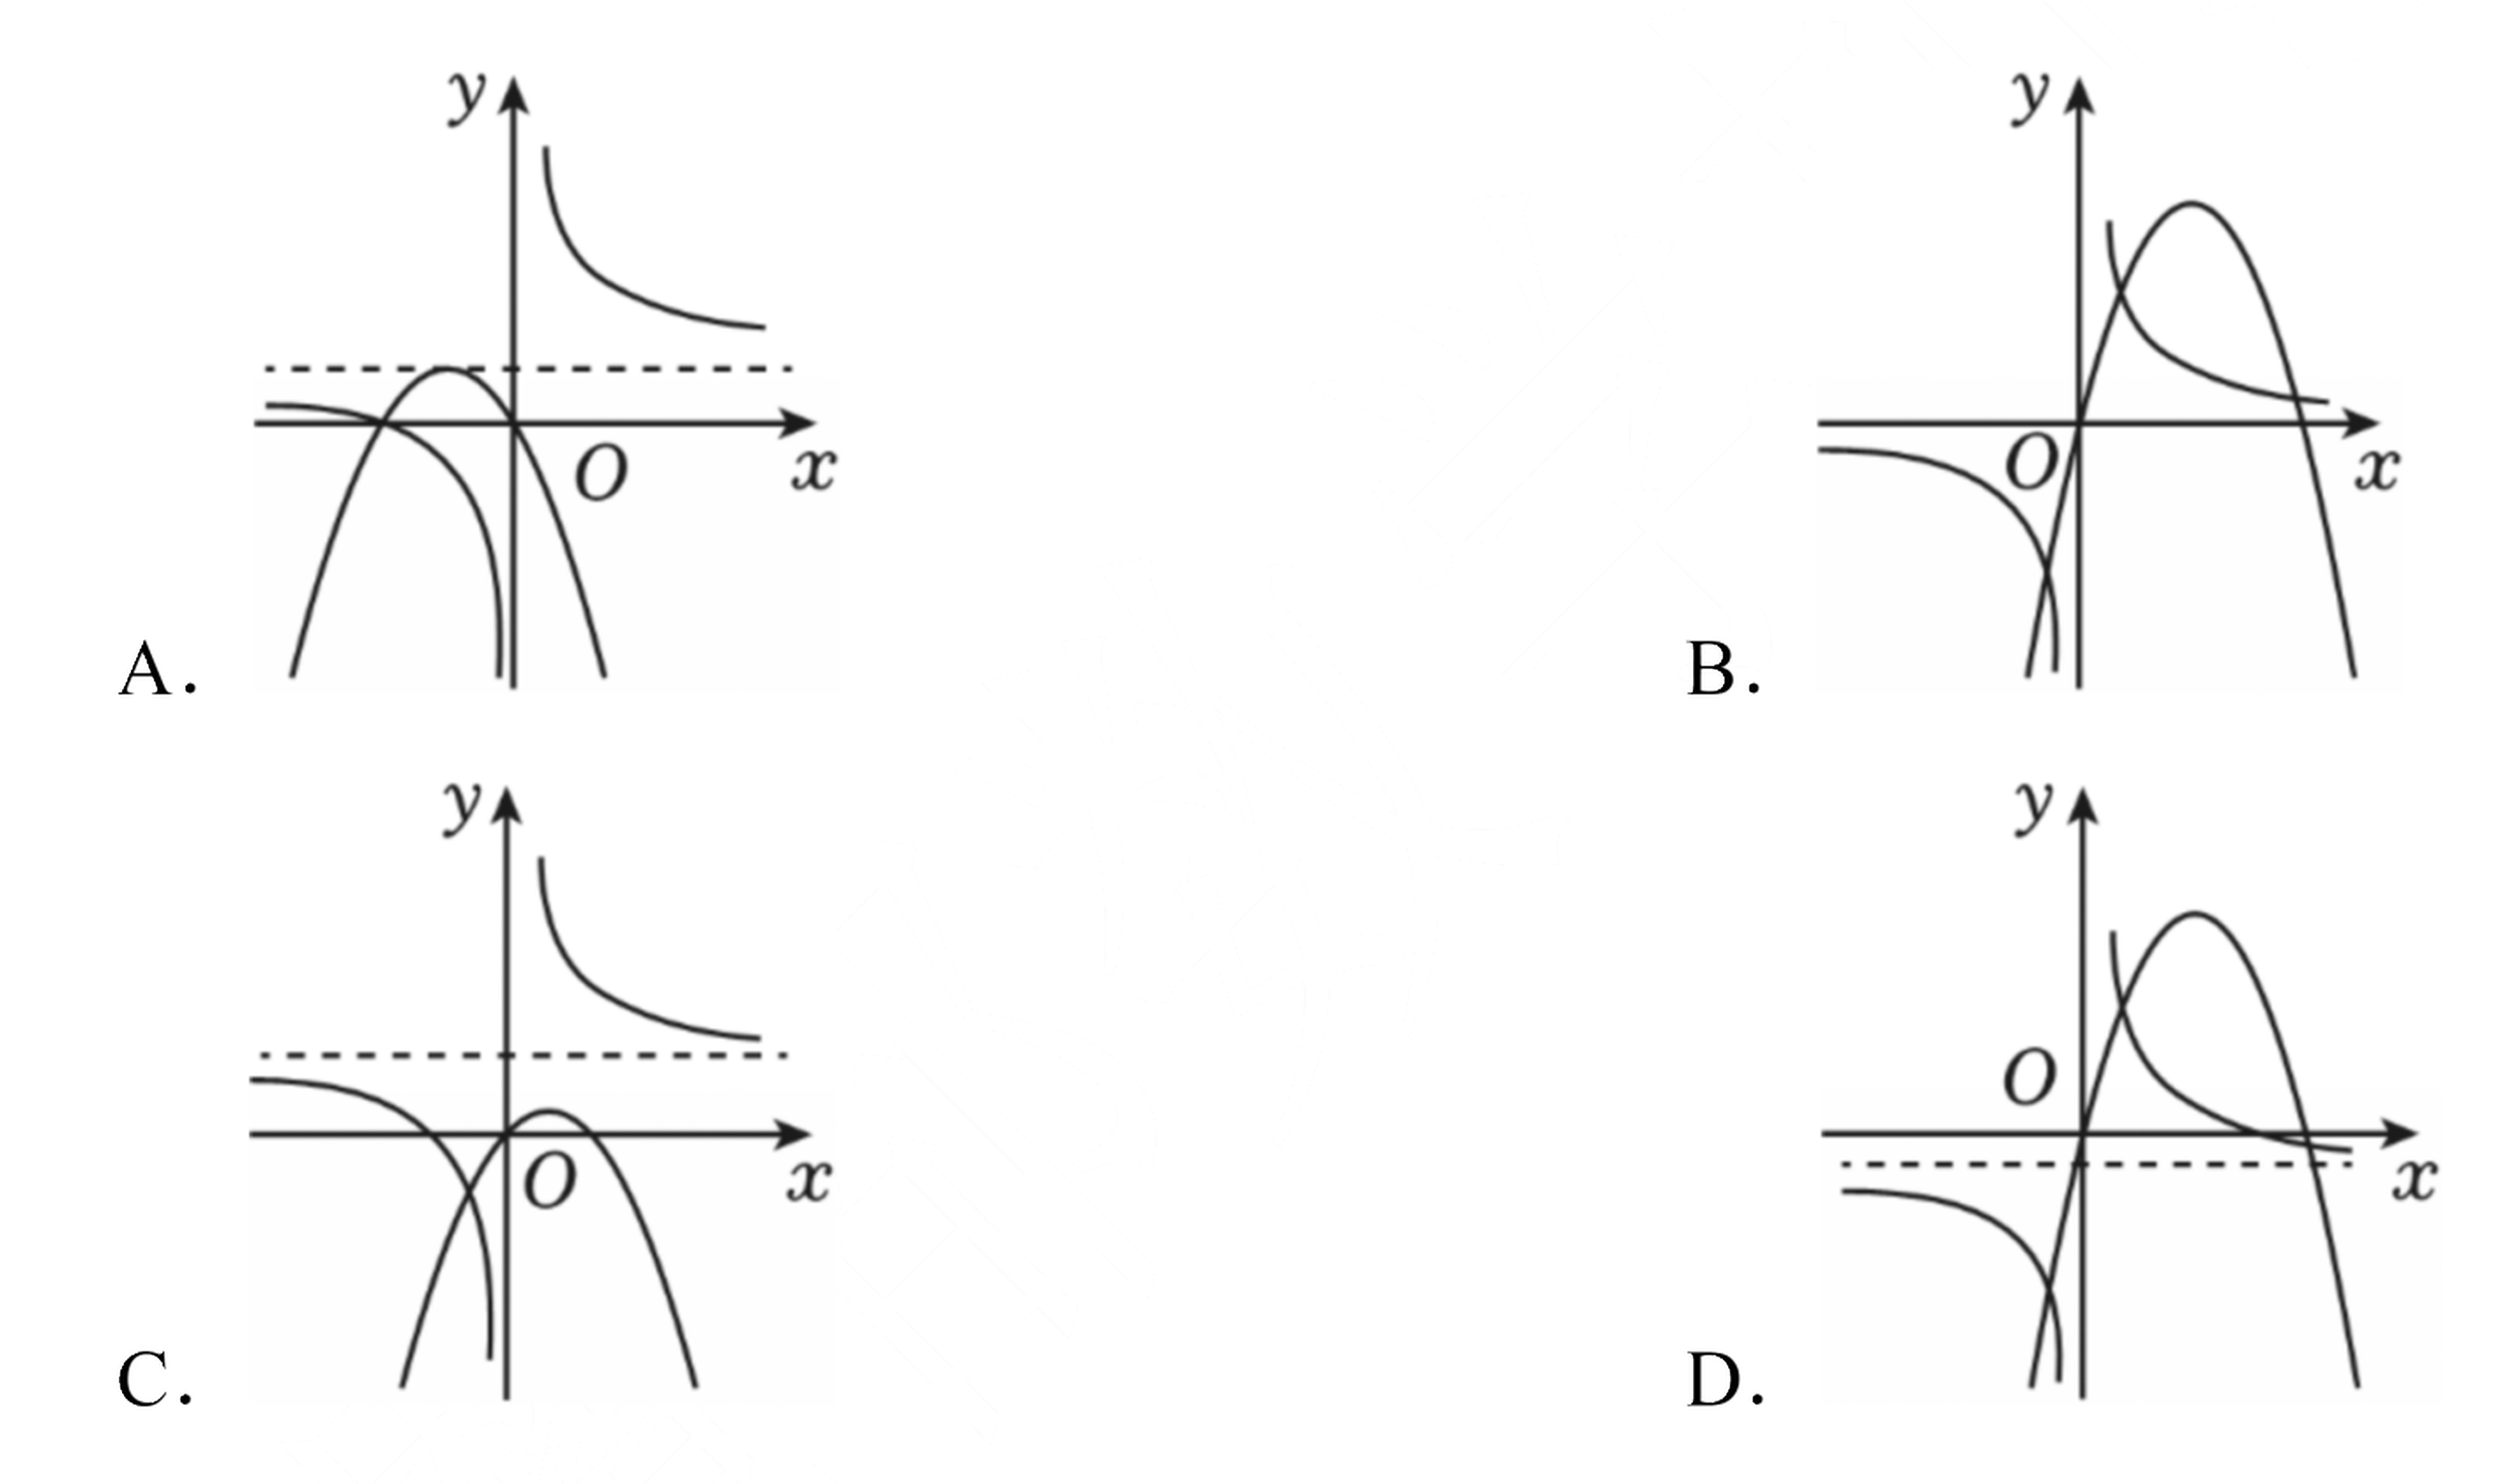
\includegraphics[width=0.80\textwidth]{figures/gao161_q14.png}
\end{center}

\ifanswer
\solbegin
\step{$A$ 选项，由二次函数图象得 $a<0$，$b<0$，由幂函数型函数图象得 $a<0$，$b>0$，}
\step{故 $A$ 选项错误；}
\step{$B$ 选项，由二次函数图象得 $a<0$，$b>0$，由幂函数型函数图象得 $a<0$，$b=0$，}
\step{故 $B$ 选项错误；}
\step{$C$ 选项，由二次函数图象得 $a<0$，$b>0$，由幂函数型函数图象得 $a<0$，$b>0$，}
\step{故 $C$ 选项正确；}
\step{$D$ 选项，由二次函数图象得 $a<0$，$b>0$，由幂函数型函数图象得 $a<0$，$b<0$，}
\step{故 $D$ 选项错误.}
\step{故选 $C$.}
\solend
\fi

% === Q15 === \subseteq／\subset、\varnothing、\mid；"排除 C""排除 B、D"正体字母照录；解析 4 行，故选 $A$
\item 设不等式 $\lvert f(x)\rvert+\lvert g(x)\rvert<a$（常数 $a>0$）的解集是 $M$，设不等式 $\lvert f(x)+g(x)\rvert<a$（常数 $a>0$）的解集是 $N$，则\mbox{（\quad）}

\keepwithprev
A. $M\subseteq N$\qquad B. $N\subseteq M$\qquad C. $M\subset N$\qquad D. $N\subset M$

\ifanswer
\solbegin
\step{$x\in M\Rightarrow\lvert f(x)+g(x)\rvert\leqslant\lvert f(x)\rvert+\lvert g(x)\rvert<a\Rightarrow x\in N$，所以 $M\subseteq N$.}
\step{取 $f(x)=g(x)=0$，则 $M=N$，排除 C.}
\step{取 $f(x)=1$，$g(x)=-1$，$a=1$，则 $M=\varnothing$，$N$ 为全体实数，排除 B、D.}
\step{故选 $A$.}
\solend
\fi

% === Q16 === "人文集"定义证明；cases 无；解析 21 行，故选 $B$
\item 设集合 $I_n=\{1,2,\cdots,n\}$，$n\in\N,n\geqslant1$，集合 $P_n=\left\{\dfrac{m}{\sqrt k}\mid m\in I_n,k\in I_n\right\}$，若 $P_n$ 的子集 $A$ 中任意两个元素之和不是整数的平方，则称 $A$ 为 “人文集”. 那么使 $P_n$ 能分成两个交集为空集的 “人文集” 的并集，且这两个人文集的并集恰为 $P_n$ 时，$n$ 的最大值是\mbox{（\quad）}

\keepwithprev
A. 13\qquad B. 14\qquad C. 15\qquad D. 16

\ifanswer
\solbegin
\step{先证当 $n\geqslant15$ 时，$P_n$ 不能分成两个不相交的人文集的并集.}
\step{假设当 $n\geqslant15$ 时，$P_n$ 可以分成两个不相交的人文集的并集，}
\step{设 $A$ 和 $B$ 为两个不相交的人文集，使 $A\cup B=P_n\supseteq I_n$.}
\step{不妨设 $1\in A$，则由于 $1+3=2^2$，所以 $3\notin A$，即 $3\in B$.}
\step{同理可得，$6\in A$，$10\in B$. 又推出 $15\in A$，}
\step{但 $1+15=4^2$，这与 $A$ 为人文集相矛盾.}
\step{再证 $P_{14}$ 满足要求. 当 $k=1$ 时，$P_{14}=\left\{\dfrac{m}{\sqrt k}\mid m\in I_{14},k\in I_{14}\right\}$，}
\step{可以分成 2 个人文集的并集.}
\step{事实上，只要取 $A_1=\{1,2,4,6,9,11,13\}$，$B_1=\{3,5,7,8,10,12,14\}$，}
\step{则 $A_1$ 和 $B_1$ 都是人文集，且 $A_1\cup B_1=P_{14}$.}
\step{当 $k=4$ 时，集合 $\left\{\dfrac{m}{\sqrt k}\mid m\in I_{14}\right\}$ 中，除整数外，}
\step{剩下的数组成集合 $\left\{\dfrac12,\dfrac32,\dfrac52,\cdots,\dfrac{13}{2}\right\}$，}
\step{可以分为下列 2 个人文集的并：$A_2=\left\{\dfrac12,\dfrac52,\dfrac92,\dfrac{11}{2}\right\}$，$B_2=\left\{\dfrac32,\dfrac72,\dfrac{13}{2}\right\}$.}
\step{当 $k=9$ 时，集合 $\left\{\dfrac{m}{\sqrt k}\mid m\in I_{14}\right\}$ 中，除整数外，}
\step{剩下的数组成集合 $\left\{\dfrac13,\dfrac23,\dfrac43,\dfrac53,\cdots,\dfrac{13}{3},\dfrac{14}{3}\right\}$，}
\step{可以分为下列 2 个人文集的并：$A_3=\left\{\dfrac13,\dfrac43,\dfrac53,\dfrac{10}{3},\dfrac{13}{3}\right\}$，$B_3=\left\{\dfrac23,\dfrac73,\dfrac83,\dfrac{11}{3},\dfrac{14}{3}\right\}$.}
\step{最后，集合 $C=\left\{\dfrac{m}{\sqrt k}\mid m\in I_{14},k\in I_{14},k\ne1,4,9\right\}$ 中的数的分母都是无理数，}
\step{它与 $P_n$ 中的任何其他数之和都不是整数，}
\step{因此，令 $A=A_1\cup A_2\cup A_3\cup C$，$B=B_1\cup B_2\cup B_3$，}
\step{则 $A$ 和 $B$ 是不相交的人文集，且 $A\cup B=P_{14}$.}
\step{综上，$n$ 的最大值为 14，故选 $B$.}
\solend
\fi

\end{enumerate}

\bigsec{三、解答题}

\begin{enumerate}
\setcounter{enumi}{16}

% === Q17 === "图像"照录；\Z；cases 块；解析 9 行，跨 06—07 页
\item (1) 已知函数 $y=x^{\frac{4m-m^2}{2}}$（$m\in\Z$）在区间 $(0,+\infty)$ 上是严格增函数，它的图像关于 $y$ 轴对称，求 $m$ 的值及该函数的解析式；

(2) 若 $(a-2)^{\frac32}<(1+2a)^{\frac32}$，求实数 $a$ 的取值范围.

\ifanswer
\solbegin
\step{(1) 由幂函数在 $(0,+\infty)$ 上严格递增，得 $\dfrac{4m-m^2}{2}>0\Leftrightarrow0<m<4$，}
\step{又 $m\in\Z$，所以 $m\in\{1,2,3\}$.}
\step{当 $m=1$ 或 $m=3$ 时，函数为 $y=x^{\frac32}$，定义域为 $[0,+\infty)$，}
\step{图像不关于 $y$ 轴对称.}
\step{当 $m=2$ 时，函数为 $y=x^2$，满足题意，所以 $m=2$，解析式 $y=x^2$.}
\step{(2) 原不等式有意义，须满足 $\begin{cases}a-2\geqslant0\\1+2a\geqslant0\end{cases}\Leftrightarrow a\geqslant2$，}
\step{函数 $y=x^{\frac32}$ 在 $[0,+\infty)$ 上严格递增，}
\step{因此 $(a-2)^{\frac32}<(1+2a)^{\frac32}\Leftrightarrow a-2<1+2a\Leftrightarrow a>-3$，}
\step{结合 $a\geqslant2$，得 $a\in[2,+\infty)$.}
\solend
\fi

% === Q18 === 题干"$a\geqslant0$"与解析"$a<0$"自相矛盾照录；"$A\cap B=(-2,-1]\cap[2,6)$"误印 ∩ 照录；\subseteq；解析 10 行
\item 已知实数 $a\geqslant0$，集合 $A=\left\{x\mid\dfrac{x+2}{x-6}<0\right\}$，$B=\{x\mid\lvert2x-1\rvert\geqslant3\}$，$C=\{x\mid x^2-3ax+2a^2<0\}$，

(1) 求 $A\cap B$；

(2) 若 $C\subseteq(A\cap B)$，求 $a$ 的取值范围.

\ifanswer
\solbegin
\step{(1) 由 $\dfrac{x+2}{x-6}<0$ 得 $-2<x<6$，即 $A=\{x\mid-2<x<6\}=(-2,6)$，}
\step{由 $\lvert2x-1\rvert\geqslant3$ 得 $2x-1\geqslant3$ 或 $2x-1\leqslant-3$，解得 $x\geqslant2$ 或 $x\leqslant-1$，}
\step{即 $B=(-\infty,-1]\cup[2,+\infty)$，}
\step{所以 $A\cap B=(-2,-1]\cap[2,6)$；}% 原卷把 ∪ 误印成 ∩，照录未改（见 ⑤ 2）
\step{(2) 由 (1) 得 $A\cap B=\{x\mid-2<x\leqslant-1\text{ 或 }2\leqslant x<6\}$，}
\step{因为 $C\subseteq(A\cap B)$，$x^2-3ax+2a^2=(x-a)(x-2a)<0$，}% 题干 $a\geqslant0$ 与解析 $a<0$ 自相矛盾，照录未改（见 ⑤ 1）
\step{当 $a=0$ 时，$C=\varnothing$，符合题意；}
\step{当 $a>0$ 时，$C=(a,2a)$，则 $\begin{cases}a\geqslant2\\2a\leqslant6\\a>0\end{cases}$，解得 $2\leqslant a\leqslant3$，}
\step{当 $a<0$ 时，$C=(2a,a)$，则 $\begin{cases}2a\geqslant-2\\a\leqslant-1\\a<0\end{cases}$，解得 $a=-1$，}
\step{故 $a$ 的范围为 $\{-1,0\}\cup[2,3]$.}
\solend
\fi

% === Q19 === 双碳太阳能应用题；"双碳""自发自用、市电互补"弯引号；解析 8 行，跨 08 页上下
\item 为响应 “双碳” 目标，某电子企业拟安装一套可使用 10 年的太阳能供电设备. 该设备的安装费用 $P(x)$（单位：万元）与太阳能电池板面积 $x(x>0)$（单位：平方米）成正比，比例系数为 $\dfrac12$. 为保障生产用电，安装后采用 “自发自用、市电互补” 模式，在此模式下，企业每年消耗的电费 $Q(x)$（单位：万元）与安装的这种太阳能电池板的面积 $x$ 之间的函数关系是 $Q(x)=\dfrac{180}{x+5}$. 记 $W(x)$（单位：万元）为该企业安装这种太阳能供电设备的费用与 10 年所消耗的电费之和.

(1) 要使该设备的安装费与第 1 年的电费之和不超过 17 万元，求安装太阳能电池板面积 $x$ 的取值范围；

(2) 当 $x$ 为多少平方米时，$W(x)$ 取得最小值？最小值是多少万元？

\ifanswer
\solbegin
\step{(1) $P(x)=\dfrac{x}{2}$，安装费与第 1 年的电费之和不超过 17 万元，即 $\dfrac{x}{2}+\dfrac{180}{x+5}\leqslant17$，}
\step{$x>0$，上式等价于 $x^2-29x+190\leqslant0\Leftrightarrow(x-10)(x-19)\leqslant0$，}
\step{解得 $x\in[10,19]$.}
\step{(2) 安装费用与 10 年电费之和为 $W(x)=P(x)+10Q(x)$，}
\step{$=\dfrac{x}{2}+\dfrac{1800}{x+5}=\dfrac{x+5}{2}+\dfrac{1800}{x+5}-\dfrac52$，}
\step{$x>0$，由基本不等式得 $W(x)\geqslant2\sqrt{\dfrac{x+5}{2}\cdot\dfrac{1800}{x+5}}-\dfrac52=60-\dfrac52=57.5$，}
\step{等号当且仅当 $\dfrac{x+5}{2}=\dfrac{1800}{x+5}$，即 $x=55$ 时成立.}
\step{因此，当电池板面积为 55 平方米时，$W(x)$ 取得最小值 57.5 万元.}
\solend
\fi

% === Q20 === $a*b$ 定义；\min 改正体；cases 块；解析 23 行，跨 08—10 页
\item 设 $a$、$b\in\R$，定义 $a*b=\begin{cases}a,&a<b\\b,&a\geqslant b\end{cases}$.

(1) 若 $x*2>1$，求 $x$ 的取值范围；

(2) 若 $(\lvert x-1\rvert+\lvert x-2\rvert)*3=3$，求 $x$ 的取值范围；

(3) 若 $a$、$b>0$，记 $M=a*\dfrac{b}{a^2+4b^2}$，分别比较 $M$ 与 $a$，以及 $M$ 与 $\dfrac{b}{a^2+4b^2}$ 的大小，并求 $M$ 的最大值.

\ifanswer
\solbegin
\step{(1) 定义 $a*b=\begin{cases}a,&a<b\\b,&a\geqslant b\end{cases}$，由 $x*2>1$，得 $\begin{cases}x<2\\x>1\end{cases}$，或 $\begin{cases}x\geqslant2\\2>1\end{cases}$，}
\step{解得 $x>1$，即 $x$ 的取值范围为 $\{x\mid x>1\}$；}
\step{(2) 当 $x\geqslant2$ 时，$\lvert x-1\rvert+\lvert x-2\rvert=2x-3\geqslant1$，}
\step{当 $1\leqslant2x-3\leqslant3$，即 $2\leqslant x\leqslant3$ 时，}
\step{此时 $(\lvert x-1\rvert+\lvert x-2\rvert)*3=2x-3=3$，解得 $x=3$；}
\step{当 $2x-3>3$，即 $x>3$ 时，}
\step{此时 $(\lvert x-1\rvert+\lvert x-2\rvert)*3=3$ 恒成立，则 $x>3$；}
\step{当 $-2x+3>3$，即 $x<0$ 时，}
\step{此时 $(\lvert x-1\rvert+\lvert x-2\rvert)*3=3$ 恒成立，则 $x<0$.}
\step{当 $1<x<2$ 时，$\lvert x-1\rvert+\lvert x-2\rvert=1$，}
\step{此时 $(\lvert x-1\rvert+\lvert x-2\rvert)*3=1\ne3$，不符合题意；}
\step{当 $x\leqslant1$ 时，$\lvert x-1\rvert+\lvert x-2\rvert=-2x+3\geqslant1$，}
\step{当 $-2x+3\leqslant3$，即 $0\leqslant x\leqslant1$ 时，}
\step{此时 $(\lvert x-1\rvert+\lvert x-2\rvert)*3=-2x+3=3$，解得 $x=0$.}
\step{综上所述，$x$ 的取值范围为 $\{x\mid x\leqslant0\text{ 或 }x\geqslant3\}$；}
\step{(3) 由题意，$M=a*\dfrac{b}{a^2+4b^2}=\min\left\{a,\dfrac{b}{a^2+4b^2}\right\}$，}% 原卷印斜体 min，按全稿惯例改正体 \min（见 ② ⑬）
\step{则 $M\leqslant a$，$M\leqslant\dfrac{b}{a^2+4b^2}$.}
\step{因为 $a$、$b>0$，所以 $\dfrac{b}{a^2+4b^2}\leqslant\dfrac{b}{2\sqrt{a^2\cdot4b^2}}=\dfrac{1}{4a}$，}
\step{当且仅当 $a=2b>0$ 时取等号，}
\step{当 $a\geqslant\dfrac{1}{4a}$，即 $a\geqslant\dfrac12$ 时，$M=a*\dfrac{b}{a^2+4b^2}=\dfrac{b}{a^2+4b^2}\leqslant\dfrac{1}{4a}$，}
\step{则 $a=\dfrac12$，$b=\dfrac14$ 时，$M$ 取得最大值 $\dfrac12$；}
\step{当 $0<a<\dfrac12$ 时，$M=a*\dfrac{b}{a^2+4b^2}=a$，此时 $M<\dfrac12$.}
\step{综上所述，$M$ 的最大值为 $\dfrac12$.}
\solend
\fi

% === Q21 === $A_n$／$B_n$／$S_n$／$T_n$ 新定义；题干第 3 问误标 (2) 照录、解析作 (3)；\prec；解析 25 行，跨 10—11 页
\item 对任意正整数 $n$，记集合 $A_n=\{(a_1,a_2,\cdots,a_n)\mid a_1,a_2,\cdots,a_n$ 均为非负整数，且 $a_1+a_2+\cdots+a_n=n\}$，集合 $B_n=\{(b_1,b_2,\cdots,b_n)\mid b_1,b_2,\cdots,b_n$ 均为非负整数，且 $b_1+b_2+\cdots+b_n=2n\}$. 设 $\alpha=(a_1,a_2,\cdots,a_n)\in A_n$，$\beta=(b_1,b_2,\cdots,b_n)\in B_n$，若对任意 $i\in\{1,2,\cdots,n\}$ 都有 $a_i\leqslant b_i$，则记 $\alpha\prec\beta$.

(1) 写出集合 $A_2$ 和 $B_2$；

(2) 证明：对任意 $\alpha\in A_n$，存在 $\beta\in B_n$，使得 $\alpha\prec\beta$；

(2) 设集合 $S_n=\{(\alpha,\beta)\mid\alpha\in A_n,\beta\in B_n,\alpha\prec\beta\}$，求证：$S_n$ 中的元素个数是完全平方数.% 原卷第 3 问题干误标 (2)（与第 2 问重号），照录未改（见 ⑤ 3）

\ifanswer
\solbegin
\step{(1) $A_2=\{(0,2),(1,1),(2,0)\}$，$B_2=\{(0,4),(1,3),(2,2),(3,1),(4,0)\}$；}
\step{(2) 对任意 $\alpha=(a_1,a_2,\cdots,a_n)\in A_n$，设 $b_i=a_i+1$（$i=1,2,3,\cdots,n$），}
\step{则 $b_1,b_2,\cdots,b_n$ 均为非负整数，且 $a_i\leqslant b_i$（$i=1,2,3,\cdots,n$）.}
\step{令 $\beta=(b_1,b_2,\cdots,b_n)$，则 $b_1+b_2+\cdots+b_n$}
\step{$=(a_1+1)+(a_2+1)+\cdots+(a_n+1)=(a_1+a_2+\cdots+a_n)+n=2n$，}
\step{所以 $\beta\in B_n$，且 $\alpha\prec\beta$.}
\step{(3) 对任意 $\alpha=(a_1,a_2,\cdots,a_n)\in A_n$，$\alpha'=(a_1',a_2',\cdots,a_n')\in A_n$，}
\step{记 $\alpha+\alpha'=(a_1+a_1',a_2+a_2',\cdots,a_n+a_n')$，}
\step{则 $a_1+a_1',a_2+a_2',\cdots,a_n+a_n'$ 均为非负整数，}
\step{且 $(a_1+a_1')+(a_2+a_2')+\cdots+(a_n+a_n')$}
\step{$=(a_1+a_2+\cdots+a_n)+(a_1'+a_2'+\cdots+a_n')=n+n=2n$，}
\step{所以 $\alpha+\alpha'\in B_n$，且 $\alpha\prec\alpha+\alpha'$，$\alpha'\prec\alpha+\alpha'$.}
\step{设集合 $A_n$ 中的元素个数为 $t$，设 $A_n=\{\alpha_1,\alpha_2,\cdots,\alpha_t\}$.}
\step{设集合 $T_n=\{(\alpha_i,\alpha_i+\alpha_j)\mid i=1,2,\cdots,t,j=1,2,\cdots,t\}$.}
\step{对任意 $\alpha_i\in A_n$（$i=1,2,\cdots,t$），都有 $\alpha_i+\alpha_1,\alpha_i+\alpha_2,\cdots,\alpha_i+\alpha_t\in B_n$，}
\step{且 $\alpha_i\prec\alpha_i+\alpha_j$，$j=1,2,\cdots,t$，所以 $T_n\subseteq S_n$.}
\step{若 $(\alpha,\beta)\in S_n$，其中 $\alpha=(a_1,a_2,\cdots,a_n)\in A_n$，$\beta=(b_1,b_2,\cdots,b_n)\in B_n$，}
\step{设 $c_i=b_i-a_i$（$i=1,2,\cdots,n$），因为 $a_i\leqslant b_i$，所以 $c_i=b_i-a_i\geqslant0$，}
\step{记 $\alpha'=(c_1,c_2,\cdots,c_n)$，}
\step{则 $c_1+c_2+\cdots+c_n=(b_1-a_1)+(b_2-a_2)+\cdots+(b_n-a_n)$}
\step{$=(b_1+b_2+\cdots+b_n)-(a_1+a_2+\cdots+a_n)=2n-n=n$，}
\step{所以 $\alpha'\in A_n$，并且有 $\beta=\alpha+\alpha'$，所以 $(\alpha,\beta)\in T_n$，所以 $S_n\subseteq T_n$，}
\step{所以 $S_n=T_n$.}
\step{因为集合 $T_n$ 中的元素个数为 $t^2$，所以 $S_n$ 中的元素个数为 $t^2$，}
\step{是完全平方数.}
\solend
\fi

\end{enumerate}

\end{document}
"
%
% ① 原始材料：微信公众号"魔都数学加油站"文章，连载"27学年高一161"，原卷卷面标题
% "2026-2027 年松江一中嘉一实验高一上期中"（卷面未印副标题、未印连载号）。
% 正文为 11 张 PNG 页（01/02/03/05/06/07/08/09/11 为 4762×6735，04/10 为
% 2560×3620，同一篇各页分辨率混排，逐页按各自分辨率裁图核对）。
% 体例：讲评版——填空 3—12（10 题）、选择 13—16（4 题）、解答 17—21（5 题），
% 共 19 题，自第 3 题起编（1、2 未印在本篇）；Q13 答案"A"直接印在题干括号内、
% 且无【答案】/【解析】段，本稿按 高一37 第 13 题／高一57 第 13 题成例把括号
% 留空、另提 \ans{$A$}；其余 18 题逐题印【解析】、用 \solbegin…\solend。
% 题目、答案、解析均据原图转录；卷面粉红色水印"魔都数学加油站"及公众号页脚未录入。
% 全卷插图清单（逐页通读 11 页确认）：仅 1 组——Q14 四幅图像选项（04 页 2×2
% 排布，二次函数与幂函数型函数在同一坐标系中的图象，A/B/C/D 四幅小图），
% 合并成一张，三版都出，裁 figures/gao161_q14.png。其余各页逐页确认无其它
% 题目配图、无解析内配图、无表格、无"如图"处（Q16 解析里的"可以分为下列 2 个
% 人文集的并"是纯文字＋集合，不是表格；OCR 里看似表格的行实为大括号与分数）。
%
% 卷首标题：原卷印作"2026-2027 年松江一中嘉一实验高一上期中"，年份区间按全稿惯例排 en dash；
% 原卷卷面未印副标题，本稿按同期中卷知识模块口径补出"集合与常用逻辑用语、不等式、函数"。
%
% ② 与原卷的排版差异／照录项清单：
%   ① 原文从第 3 题起，本稿保留原题号；共 19 题三节，解答题 5 题到 21；
%      三节各自一个 enumerate + \setcounter{enumi}{2}/{12}/{16}（不贯穿），
%      用 \examtitlest[3] 起手；
%   ② 混合体例：Q13 原卷把答案"A"直接印在题干括号内（"（  A  ）"）、且题下
%      无【答案】/【解析】段，按 高一37 第 13 题／高一57 第 13 题成例把括号
%      留空、另提 \ans{$A$}、不补造解析；其余 18 题印【解析】、用
%      \solbegin…\solend；四道选择题中 Q14/Q15/Q16 的答案在解析末句
%      "故选 $C$／$A$／$B$"、Q13 用 \ans{$A$}；括号 \mbox{（\quad）} 留空；
%      答案版【答案】/【解析】标记数 = 19 = 全卷题数（1 个 \ans ＋ 18 个 \solbegin）；
%   ③ 原卷卷面未印副标题，本稿按知识模块口径补出；
%   ④ 原卷填空横线按全稿惯例排 \blankline[4.4em]；选择题选项段前按惯例各加
%      \keepwithprev；Q14 四幅选项图整块用 \needvspace{9cm} 守卫（守卫放
%      \item 之前，见 高一132 Q14／高一154 Q15 成例）；解答题不留作答区、
%      不加 \anspace（原卷为讲评版）；
%   ⑤ 数集归一：Q8"$x\in\R$"、Q11"$m\in\R$"、Q13"$x,y\in\N$"、
%      Q16"$n\in N$"、Q17"$m\in\Z$"、Q20"$a$、$b\in R$"——原卷印正体粗体
%      或斜体 R/N/Z，按全稿惯例归一 \R／\N／\Z；绝对值排 \lvert…\rvert
%      （Q9、Q12、Q15、Q18、Q20），集合描述竖线排 \mid（Q12、Q16、Q18、
%      Q20、Q21），空集 \varnothing（Q15、Q18），补集无用例，不等号按全稿
%      惯例排 \leqslant／\geqslant；
%   ⑥ 子集符号逐处照录不统一：Q12 cases 定义"$C(A)\geqslant C(B)$"、
%      Q15 选项 A/B"$M\subseteq N$""$N\subseteq M$"与解析"$M\subseteq N$"
%      印带下划线 ⊆（照录 \subseteq），Q15 选项 C/D"$M\subset N$""$N\subset M$"
%      印单线 ⊂（照录 \subset），Q18 "$C\subseteq(A\cap B)$"、Q21
%      "$T_n\subseteq S_n$""$S_n\subseteq T_n$"均带下划线照录 \subseteq；
%      本卷无 \not\subset 用例；
%   ⑦ 判别式：Q7 解析"$\Delta=(m-6)(m+2)>0$"、Q8 解析"$\Delta=a^2-4a<0$"、
%      Q12 解析"$\Delta=a^2-8$"共 3 处，逐处放大确认印等腰偏高粗三角
%      （高>宽、右斜边粗），照录 \Delta；本卷无扁等边细线 \triangle 用例；
%   ⑧ 中文弯引号照录：Q7"$m\geqslant6$""有两个不相等的正实数根"及四个
%      条件短语、Q13 反证法命题、Q16"人文集"、Q19"双碳""自发自用、市电互补"；
%      注释里一律 ASCII 引号；数学式内 CJK 用 \text{}（Q18、Q20 解集描述内"或"）；
%   ⑨ "图像／图象"逐处照录不统一：Q4"的图像"、Q17 题干"它的图像关于 $y$ 轴
%      对称"及解析"图像不关于 $y$ 轴对称"印"图像"；Q14 题干"的图象可能为"
%      与解析 A/B/C/D 四行各"由二次函数图象得""由幂函数型函数图象得"
%      共 8 处印"图象"（象，无亻）；
%   ⑩ 文本圈数字逐处照录：Q12 题干①②③④、Q12 解析"故①错误""故②正确"
%      "故③正确""故④错误""故正确的是②③"，均为印刷圈数字（文本模式）；
%   ⑪ 半角逗号在数学组之间是全稿惯例、非笔误，逐处照录（Q5"$a$、$b$"、
%      Q13"$x,y\in\N$"、Q16"$n\in\N,n\geqslant1$"与集合描述内逗号、
%      Q20"$a,b\in\R$"、Q21 各集合描述内逗号）；行末西文句点 ASCII `.`；
%      原卷行中句点（Q16"$10\in B$. 又推出 $15\in A$"、Q16"再证 $P_{14}$
%      满足要求. 当 $k=1$ 时"、Q18"$A\cap B=(-2,-1]\cap[2,6)$；"后的分号）
%      按全稿惯例一律排 ASCII `.`／全角"；"；中文语境行中全角逗号／顿号照录；
%   ⑫ 原卷数学式内联条件（Q14"$y=x^a+b(a\ne0)$"、Q19"$x(x>0)$"、
%      Q11"$\lvert x-m\rvert<n\,(m\in\R,n>0)$"）印半角括号，逐处照录未改
%      全角（同 高一147 口径）；
%      中文语境的括注（Q5"结果用 $a$、$b$ 表示"、Q7"填…"、Q12"填写序号"、
%      Q15"常数 $a>0$"、Q19"单位：万元"）印全角括号，照录；
%   ⑬ 复杂式照录别简化：Q3 $(a^{2-\sqrt3})^{2+\sqrt3}\times\sqrt{a^2}\times
%      b^{\sqrt3}\times b^{1-\sqrt3}$ 与 $a^{(2-\sqrt3)(2+\sqrt3)}\cdot a\cdot
%      b^{\sqrt3+1-\sqrt3}=a\cdot a\cdot b=a^2b$（题干用 \times、解析用 \cdot，
%      逐处照录不统一，见 ⑤）；Q5 $\dfrac{\lg2}{\lg2+\lg3}=\dfrac{a}{a+b}$、
%      Q10 $t-\dfrac3t=2$ 与 $b=a^3$、$ab=a^4=2$、Q11 $\left(2a-\dfrac12
%      -a+\dfrac12,2a-\dfrac12+a-\dfrac12\right)=(a,3a-1)$ 与
%      $\left(\dfrac43,\dfrac53\right]\cup\{2\}$、Q16 各分数集合、Q19
%      $x^2-29x+190\leqslant0$ 与 $W(x)=P(x)+10Q(x)$ 与
%      $2\sqrt{\dfrac{x+5}{2}\cdot\dfrac{1800}{x+5}}-\dfrac52=60-\dfrac52=57.5$、
%      Q20 $M=a*\dfrac{b}{a^2+4b^2}=\min\left\{a,\dfrac{b}{a^2+4b^2}\right\}$
%      与 $\dfrac{b}{2\sqrt{a^2\cdot4b^2}}=\dfrac{1}{4a}$、Q21 各 $A_n$／$B_n$／
%      $T_n$ 定义；\left…\right 不得拆到不同 $…$ 组（Q11 的 \left(…\right)、
%      Q11 的 \left(\dfrac43,\dfrac53\right]、Q16 的 \left\{\dfrac{m}{\sqrt k}
%      \mid…\right\} 与 \left\{\dfrac12,\dfrac32,\dfrac52,\cdots,\dfrac{13}{2}\right\}
%      等、Q20 的 \min\left\{…\right\}）；cases 块整体算一个印刷行
%      （Q12 定义、Q17 (2)、Q18 (2) 两处、Q20 定义与 (1)）；原卷 Q20 解析
%      "$=min\{…\}$"印斜体 min，按 高一122／高一102 成例改正体 \min；
%   ⑭ 一条 \step = 原卷解析的一个印刷行；别并折行、别拆行。跨页续印按题合并
%      （Q6 的 01 页上下题干重复印、Q10 的 01—02 页、Q11 的 02—03 页、
%      Q12 的 03—04 页、Q16 的 05—06 页、Q17 的 06—07 页、Q18 的 07 页
%      上下、Q19 的 08 页上下、Q20 的 08—10 页、Q21 的 10—11 页）；
%      跨半页重叠行（Q10"令 $t=\log_a b>0$…"、Q16"它与 $P_n$ 中的任何
%      其他数之和都不是整数，"、Q18"【解析】(1) 由 $\dfrac{x+2}{x-6}<0$…"、
%      Q19"$x>0$，上式等价于…"、Q20"此时…则 $x<0$."、Q21"若 $(\alpha,\beta)
%      \in S_n$…"与"设 $c_i=b_i-a_i$…"）只算一个印刷行；
%   ⑮ 自定义记号照录：Q12"$C(A)$""$A*B$""$S$"、Q16"$I_n$""$P_n$""人文集"
%      "$A_1$／$B_1$／$A_2$／$B_2$／$A_3$／$B_3$／$C$"、Q20"$a*b$""$M$"、
%      Q21"$A_n$／$B_n$／$S_n$／$T_n$""$\alpha\prec\beta$""$\alpha+\alpha'$"；
%   ⑯ 选项字母体例照录不统一：Q15 解析"排除 C.""排除 B、D."两处原卷印
%      正体（文本模式），Q13 \ans{$A$}、Q14"$A$ 选项"…"故选 $C$"、
%      Q15"故选 $A$"、Q16"故选 $B$"用斜体（数学模式），逐处照录、不统一；
%   ⑰ 红字：全卷逐页扫描无红色加粗小标题（仅粉色水印），故本卷无 \stepm，
%      不引入红色定义；
%
% ③ 行数复核：一条 \step = 原卷解析的一个印刷行，cases 块作一个印刷行计。
%   逐题数（逐页核对定稿）：Q3：1；Q4：1；Q5：1；Q6：3；Q7：4；Q8：4；
%   Q9：2；Q10：2；Q11：7；Q12：8；Q13：0（答案印括号内、提 \ans{}，
%   不计入 \step 账）；Q14：9；Q15：4；Q16：21；Q17：9；Q18：10；Q19：8；
%   Q20：23；Q21：25。
%   合计 142 行（142 条 \step，无 \stepm），与原卷逐题印刷行相等。
%   全卷 19 题：Q13 一处 \ans{} ＋ 其余 18 题设 \solbegin…\solend，
%   答案版【答案】/【解析】标记数 = 19 = 全卷题数。
%
% ④ 页码分布（供回原图复核）：
%   卷首标题＋"一、填空题"＋Q3/Q4/Q5 题干＋解析各 1 行＋Q6 题干首行
%   在 01 页上半；Q6 题干（重复印）＋解析 3 行＋Q7 题干＋解析 4 行在
%   01 页下半；Q8 题干＋解析 4 行＋Q9 题干＋解析 2 行＋Q10 题干＋
%   解析首行在 02 页上半；Q10 解析（重复印）＋末行＋Q11 题干＋解析
%   前 3 行在 02 页下半；Q11 解析后 4 行＋Q12 题干＋cases 定义＋①
%   在 03 页上半；Q12 ②③④ 三命题＋"填写序号"行＋解析前 6 行在
%   03 页下半；Q12 解析后 2 行＋"二、选择题"标题＋Q13 题干＋选项＋
%   Q14 题干＋"（　）"＋A/B 两幅图在 04 页上半；Q14 四幅图（重复印）
%   ＋解析 9 行在 04 页下半；Q15 题干＋选项＋解析 4 行＋Q16 题干＋
%   选项在 05 页上半；Q16 题干（重复印）＋选项＋解析前 10 行在 05 页
%   下半；Q16 解析中 8 行（k=4、k=9 两批＋集合 C＋"它与 $P_n$…"）
%   在 06 页上半；Q16 解析"它与 $P_n$…"（重复印）＋末 3 行＋
%   "三、解答题"标题＋Q17 题干＋两问＋解析前 4 行在 06 页下半；
%   Q17 解析后 5 行＋Q18 题干＋两问＋解析首行在 07 页上半；Q18 解析
%   （重复首行）＋余 9 行在 07 页下半；Q19 题干＋两问＋解析前 2 行在
%   08 页上半；Q19 解析（重复第 2 行）＋余 6 行＋Q20 定义＋(1) 问在
%   08 页下半；Q20 (2)(3) 两问＋解析 (1) 2 行＋(2) 前 7 行在 09 页
%   上半；Q20 解析 (2) 余 4 行＋(3) 前 4 行在 09 页下半；Q20 解析 (3)
%   余 4 行＋Q21 题干＋三问在 10 页上半；Q21 题干（重复印）＋解析
%   (1)(2)(3) 前 8 行在 10 页下半；Q21 解析 (3) 中 10 行在 11 页上半；
%   Q21 解析 (3)（重复 2 行）＋末 7 行"是完全平方数."在 11 页下半。
%   本稿按题连排，不丢行、不并折行；全卷末题为第 21 题，无附加题节。
%
% ⑤ 存疑照录（放大原图确认，照录未改、正文对应处另有 % 注）：
%   1. Q18 题干印"已知实数 $a\geqslant0$"，解析却另设"当 $a<0$ 时"并解出
%      $a=-1$，末行答案"故 $a$ 的范围为 $\{-1,0\}\cup[2,3]$"含负数，
%      与题干 $a\geqslant0$ 自相矛盾——系原卷前后不一，照录未改（放大
%      07 页确认题干确印 $a\geqslant0$）；
%   2. Q18 解析"所以 $A\cap B=(-2,-1]\cap[2,6)$；"原卷把并集误印成
%      交集号 ∩（紧接下一行"$A\cap B=\{x\mid-2<x\leqslant-1$ 或
%      $2\leqslant x<6\}$"用"或"），照录未改（放大 07 页确认印 ∩）；
%   3. Q21 题干第 3 问原卷标号印作"(2)"（与第 2 问重号），而解析里
%      同一问标作"(3)"——原卷笔误，题干与解析逐处照录、不统一；
%   4. Q3 题干四处乘号印"×"（\times）、解析内三处乘号印"·"（\cdot），
%      逐处照录未统一（放大 01 页确认）；
%   5. Q16 解析"先证当 $n\geqslant15$ 时"印 ≥（非 >），与"综上，$n$
%      的最大值为 14"自洽，照录；题干"$n\in N,n\geqslant1$"印斜体
%      $N$、按全稿惯例归一 \N（见 ② ⑤）；
%   6. Q20 解析"$M=a*\dfrac{b}{a^2+4b^2}=min\{…\}$"原卷印斜体 min，
%      按全稿惯例改正体 \min（见 ② ⑬）；末行"$M$ 的最大值为
%      $\dfrac12$"照录；
%   7. Q15 解析"排除 C.""排除 B、D."用正体字母，而"故选 $A$"用斜体
%      字母，原卷体例不一（见 ② ⑯），照录未统一。
%   全卷除此 7 类外未发现其它笔误／自相矛盾处；Q13 只把答案印在括号内、
%   其余 18 题全部印【解析】。
%

\documentclass[a4paper,11pt]{article}
\usepackage{common}

\begin{document}

\examtitlest[3]{2026--2027 年松江一中嘉一实验高一上期中}{集合与常用逻辑用语、不等式、函数}

\bigsec{一、填空题}

\begin{enumerate}
\setcounter{enumi}{2}

% === Q3 === 题干 \times、解析 \cdot 逐处照录；解析 1 行
\item 设 $a>0$，$b>0$，化简 $(a^{2-\sqrt3})^{2+\sqrt3}\times\sqrt{a^2}\times b^{\sqrt3}\times b^{1-\sqrt3}=$\blankline[4.4em].

\ifanswer
\solbegin
\step{因为 $a>0$，所以 $\sqrt{a^2}=a$，原式 $=a^{(2-\sqrt3)(2+\sqrt3)}\cdot a\cdot b^{\sqrt3+1-\sqrt3}=a\cdot a\cdot b=a^2b$.}
\solend
\fi

% === Q4 === "图像"照录；解析 1 行
\item 若幂函数 $y=x^a$ 的图像经过点 $(5,\sqrt5)$，则此幂函数的表达式为 $y=$\blankline[4.4em].

\ifanswer
\solbegin
\step{$5^a=\sqrt5\Rightarrow a=\dfrac12$，所以 $y=\sqrt x$.}
\solend
\fi

% === Q5 === "结果用 $a$、$b$ 表示"全角括号＋顿号照录；解析 1 行
\item 已知 $\lg2=a$，$10^b=3$，则 $\log_6 2=$\blankline[4.4em]（结果用 $a$、$b$ 表示）.

\ifanswer
\solbegin
\step{$\lg3=b$，$\log_6 2=\dfrac{\lg2}{\lg2+\lg3}=\dfrac{a}{a+b}$.}
\solend
\fi

% === Q6 === 对称中心；解析 3 行，题干跨 01 页上下重复印
\item 若函数 $y=\dfrac{mx-1}{x+n}$ 的对称中心是 $(4,-3)$，则 $m+n=$\blankline[4.4em].

\ifanswer
\solbegin
\step{令 $x=-n+t$（$t\ne0$），则 $y-m=-\dfrac{mn+1}{t}$；}
\step{将 $t$ 换成 $-t$，$y-m$ 变为其相反数，因此对称中心为 $(-n,m)$.}
\step{于是 $n=-4$，$m=-3$，得 $m+n=-7$.}
\solend
\fi

% === Q7 === 充要条件；中文弯引号＋圈选条件；\Delta 高瘦；解析 4 行
\item 已知关于 $x$ 的一元二次方程 $x^2-mx+m+3=0$，则 “$m\geqslant6$” 是该方程 “有两个不相等的正实数根” 的\blankline[4.4em]条件（填 “充分不必要”、“必要不充分”、“充要” 或 “既不充分也不必要”）.

\ifanswer
\solbegin
\step{方程有两个不相等的正实数根}
\step{$\Leftrightarrow m>0$、$m+3>0$ 且 $\Delta=(m-6)(m+2)>0\Leftrightarrow m>6$.}
\step{$m>6\Rightarrow m\geqslant6$，但 $m=6$ 时方程有两个相等的正实数根，}
\step{因此为必要不充分条件.}
\solend
\fi

% === Q8 === \R、\Delta；解析 4 行
\item 对于任意的 $x\in\R$，代数式 $\lg(ax^2+ax+1)$ 都有意义，则实数 $a$ 的取值范围是\blankline[4.4em].

\ifanswer
\solbegin
\step{真数须满足 $ax^2+ax+1>0$ 对任意 $x\in\R$ 恒成立.}
\step{$a=0$ 时成立；}
\step{$a\ne0$ 时，恒成立等价于 $a>0$ 且 $\Delta=a^2-4a<0$，解得 $0<a<4$；}
\step{因此 $a\in[0,4)$.}
\solend
\fi

% === Q9 === 绝对值 \lvert…\rvert；解析 2 行
\item 若不等式 $\lvert x+1\rvert-\lvert x-4\rvert<m$ 的解集为非空集合，则实数 $m$ 的取值范围是\blankline[4.4em].

\ifanswer
\solbegin
\step{$\lvert x+1\rvert-\lvert x-4\rvert\geqslant-\lvert(x+1)-(x-4)\rvert=-5$，当 $x=-1$ 时取等号，}
\step{因此原不等式的解集非空 $\Leftrightarrow m>-5$，所求范围为 $(-5,+\infty)$.}
\solend
\fi

% === Q10 === 换底；$\log_2 a\cdot\log_2 b$；解析 2 行，跨 02 页上下
\item 已知 $a>1$，$b>1$，若 $\log_a b-3\log_b a=2$，且 $ab=2$，则 $\log_2 a\cdot\log_2 b=$\blankline[4.4em].

\ifanswer
\solbegin
\step{令 $t=\log_a b>0$，则 $t-\dfrac{3}{t}=2\Leftrightarrow(t-3)(t+1)=0$，得 $t=3$，}
\step{于是 $b=a^3$，$ab=a^4=2$，得 $\log_2 a=\dfrac14$，$\log_2 b=\dfrac34$，所求为 $\dfrac{3}{16}$.}
\solend
\fi

% === Q11 === 邻域定义；\left(…\right) 不拆组；解析 7 行，跨 02—03 页
\item 对于实数 $m$ 和正数 $n$，称满足不等式 $\lvert x-m\rvert<n\,(m\in\R,n>0)$ 的实数 $x$ 的集合叫做 $m$ 的 $n$ 邻域. 已知 $a>\dfrac12$，若 $2a-\dfrac12$ 的 $a-\dfrac12$ 邻域中恰有 2 个整数，则 $a$ 的取值范围是\blankline[4.4em].

\ifanswer
\solbegin
\step{所求邻域为 $\left(2a-\dfrac12-a+\dfrac12,2a-\dfrac12+a-\dfrac12\right)=(a,3a-1)$.}
\step{当 $\dfrac12<a\leqslant1$ 时至多含 1 个整数；}
\step{当 $a>2$ 时，区间长度 $2a-1>3$，至少含 3 个整数.}
\step{当 $1<a<2$ 时，区间必含 2，恰有两个整数等价于 $3<3a-1\leqslant4$，}
\step{即 $\dfrac43<a\leqslant\dfrac53$.}
\step{当 $a=2$ 时，区间为 $(2,5)$，恰含整数 $3,4$；}
\step{所以 $a\in\left(\dfrac43,\dfrac53\right]\cup\{2\}$.}
\solend
\fi

% === Q12 === $C(A)$／$A*B$ 定义题；①②③④ 文本圈数字；\subseteq／\subset、\Delta、\mid、\varnothing；解析 8 行
\item 用 $C(A)$ 表示非空集合 $A$ 中的元素个数. 对于集合 $A$、$B$，定义

$A*B=\begin{cases}C(A)-C(B),&C(A)\geqslant C(B)\\ C(B)-C(A),&C(A)<C(B)\end{cases}$，若 $A=\{0,1\}$，$B=\{x\mid(x^2-ax)(x^2+ax+2)=0\}$，设实数 $a$ 的所有可能取值组成的集合是 $S$，则下列说法正确的是\blankline[4.4em]（填写序号）.

① $C(B)$ 的可能值为 $2,3,4$

② 若 $A*B=2$，则 $a$ 的取值范围为 $(-\infty,-2\sqrt2)\cup(2\sqrt2,+\infty)$

③ 若 $A*B=1$，则 $C(S)=3$

④ 若 $A*B=0$，则 $a$ 的取值范围为 $(-2\sqrt2,2\sqrt2)$

\ifanswer
\solbegin
\step{$x(x-a)=0$ 的根为 $0,a$，而 $x^2+ax+2$ 在这两处的值分别为 $2,2a^2+2$，}
\step{两个因式无公共实根；后者的判别式为 $\Delta=a^2-8$.}
\step{当 $a=0$、$0<\lvert a\rvert<2\sqrt2$、$\lvert a\rvert=2\sqrt2$、$\lvert a\rvert>2\sqrt2$ 时，$C(B)$ 依次为 $1,2,3,4$，}
\step{故①错误.}
\step{$A*B=\lvert2-C(B)\rvert$，所以 $A*B=2\Leftrightarrow\lvert a\rvert>2\sqrt2$，故②正确；}
\step{$A*B=1\Leftrightarrow a\in\{-2\sqrt2,0,2\sqrt2\}$，此时 $C(S)=3$，故③正确；}
\step{$A*B=0\Leftrightarrow0<\lvert a\rvert<2\sqrt2$，即 $a\in(-2\sqrt2,0)\cup(0,2\sqrt2)$，故④错误.}
\step{故正确的是②③.}
\solend
\fi

\end{enumerate}

\needvspace{7cm}
\bigsec{二、选择题}

\begin{enumerate}
\setcounter{enumi}{12}

% === Q13 === 答案"A"原卷印在题干括号内、题下无【答案】/【解析】段；按 高一37／高一57 成例另提 \ans{}
\item 用反证法证明命题 “已知 $x>0$，$y>0$，$x,y\in\N$，如果 $xy$ 可被 7 整除，那么 $x$，$y$ 至少有一个能被 7 整除” 时，假设的内容是\mbox{（\quad）}

\keepwithprev
A. $x$、$y$ 都不能被 7 整除\qquad B. $x$、$y$ 都能被 7 整除

C. $x$、$y$ 只有一个能被 7 整除\qquad D. 只有 $x$ 不能被 7 整除

\ifanswer
\ans{$A$}
\fi

% === Q14 === 四幅图像选项（2×2 合并，三版都出）；守卫放 \item 之前；"图象"照录；解析 9 行，故选 $C$
\needvspace{9cm}
\item 函数 $y=ax^2+bx$ 与函数 $y=x^a+b(a\ne0)$ 在同一平面直角坐标系中的图象可能为\mbox{（\quad）}

\keepwithprev
\begin{center}
% 四幅图象选项取 04 页 2×2 排布合并为一张，去粉色水印、转灰度、4× LANCZOS 放大；三版都出
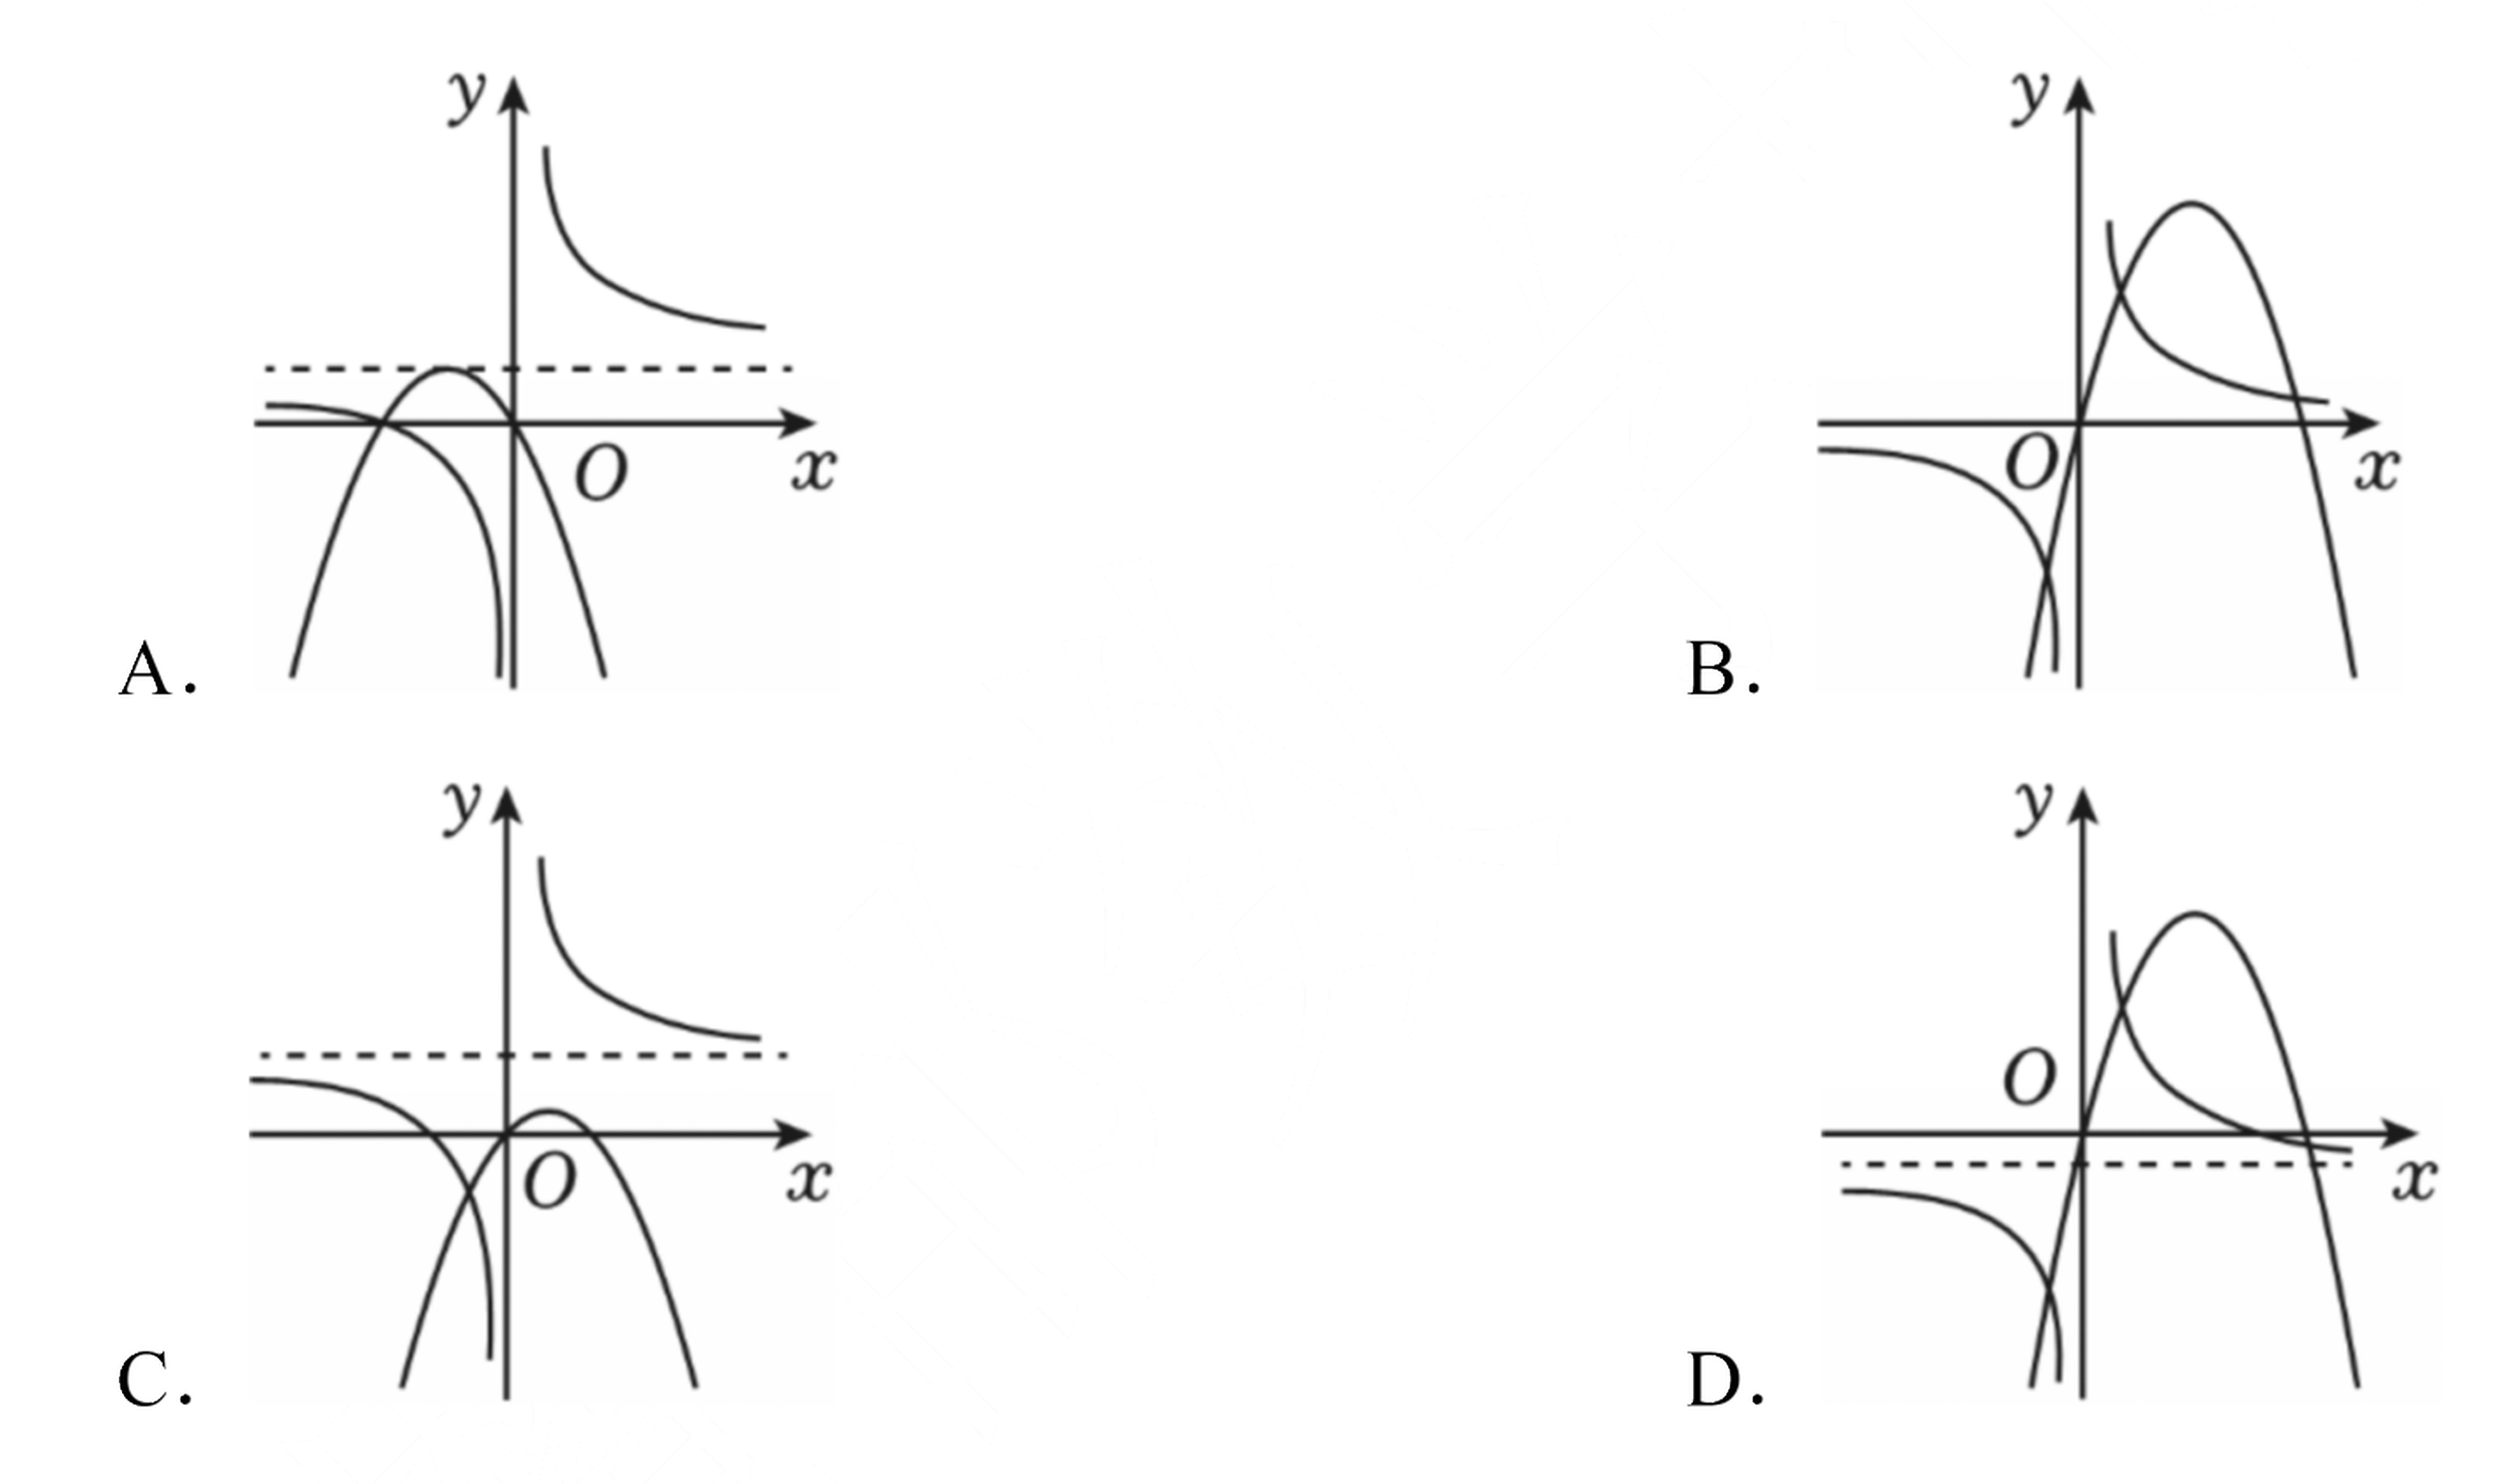
\includegraphics[width=0.80\textwidth]{figures/gao161_q14.png}
\end{center}

\ifanswer
\solbegin
\step{$A$ 选项，由二次函数图象得 $a<0$，$b<0$，由幂函数型函数图象得 $a<0$，$b>0$，}
\step{故 $A$ 选项错误；}
\step{$B$ 选项，由二次函数图象得 $a<0$，$b>0$，由幂函数型函数图象得 $a<0$，$b=0$，}
\step{故 $B$ 选项错误；}
\step{$C$ 选项，由二次函数图象得 $a<0$，$b>0$，由幂函数型函数图象得 $a<0$，$b>0$，}
\step{故 $C$ 选项正确；}
\step{$D$ 选项，由二次函数图象得 $a<0$，$b>0$，由幂函数型函数图象得 $a<0$，$b<0$，}
\step{故 $D$ 选项错误.}
\step{故选 $C$.}
\solend
\fi

% === Q15 === \subseteq／\subset、\varnothing、\mid；"排除 C""排除 B、D"正体字母照录；解析 4 行，故选 $A$
\item 设不等式 $\lvert f(x)\rvert+\lvert g(x)\rvert<a$（常数 $a>0$）的解集是 $M$，设不等式 $\lvert f(x)+g(x)\rvert<a$（常数 $a>0$）的解集是 $N$，则\mbox{（\quad）}

\keepwithprev
A. $M\subseteq N$\qquad B. $N\subseteq M$\qquad C. $M\subset N$\qquad D. $N\subset M$

\ifanswer
\solbegin
\step{$x\in M\Rightarrow\lvert f(x)+g(x)\rvert\leqslant\lvert f(x)\rvert+\lvert g(x)\rvert<a\Rightarrow x\in N$，所以 $M\subseteq N$.}
\step{取 $f(x)=g(x)=0$，则 $M=N$，排除 C.}
\step{取 $f(x)=1$，$g(x)=-1$，$a=1$，则 $M=\varnothing$，$N$ 为全体实数，排除 B、D.}
\step{故选 $A$.}
\solend
\fi

% === Q16 === "人文集"定义证明；cases 无；解析 21 行，故选 $B$
\item 设集合 $I_n=\{1,2,\cdots,n\}$，$n\in\N,n\geqslant1$，集合 $P_n=\left\{\dfrac{m}{\sqrt k}\mid m\in I_n,k\in I_n\right\}$，若 $P_n$ 的子集 $A$ 中任意两个元素之和不是整数的平方，则称 $A$ 为 “人文集”. 那么使 $P_n$ 能分成两个交集为空集的 “人文集” 的并集，且这两个人文集的并集恰为 $P_n$ 时，$n$ 的最大值是\mbox{（\quad）}

\keepwithprev
A. 13\qquad B. 14\qquad C. 15\qquad D. 16

\ifanswer
\solbegin
\step{先证当 $n\geqslant15$ 时，$P_n$ 不能分成两个不相交的人文集的并集.}
\step{假设当 $n\geqslant15$ 时，$P_n$ 可以分成两个不相交的人文集的并集，}
\step{设 $A$ 和 $B$ 为两个不相交的人文集，使 $A\cup B=P_n\supseteq I_n$.}
\step{不妨设 $1\in A$，则由于 $1+3=2^2$，所以 $3\notin A$，即 $3\in B$.}
\step{同理可得，$6\in A$，$10\in B$. 又推出 $15\in A$，}
\step{但 $1+15=4^2$，这与 $A$ 为人文集相矛盾.}
\step{再证 $P_{14}$ 满足要求. 当 $k=1$ 时，$P_{14}=\left\{\dfrac{m}{\sqrt k}\mid m\in I_{14},k\in I_{14}\right\}$，}
\step{可以分成 2 个人文集的并集.}
\step{事实上，只要取 $A_1=\{1,2,4,6,9,11,13\}$，$B_1=\{3,5,7,8,10,12,14\}$，}
\step{则 $A_1$ 和 $B_1$ 都是人文集，且 $A_1\cup B_1=P_{14}$.}
\step{当 $k=4$ 时，集合 $\left\{\dfrac{m}{\sqrt k}\mid m\in I_{14}\right\}$ 中，除整数外，}
\step{剩下的数组成集合 $\left\{\dfrac12,\dfrac32,\dfrac52,\cdots,\dfrac{13}{2}\right\}$，}
\step{可以分为下列 2 个人文集的并：$A_2=\left\{\dfrac12,\dfrac52,\dfrac92,\dfrac{11}{2}\right\}$，$B_2=\left\{\dfrac32,\dfrac72,\dfrac{13}{2}\right\}$.}
\step{当 $k=9$ 时，集合 $\left\{\dfrac{m}{\sqrt k}\mid m\in I_{14}\right\}$ 中，除整数外，}
\step{剩下的数组成集合 $\left\{\dfrac13,\dfrac23,\dfrac43,\dfrac53,\cdots,\dfrac{13}{3},\dfrac{14}{3}\right\}$，}
\step{可以分为下列 2 个人文集的并：$A_3=\left\{\dfrac13,\dfrac43,\dfrac53,\dfrac{10}{3},\dfrac{13}{3}\right\}$，$B_3=\left\{\dfrac23,\dfrac73,\dfrac83,\dfrac{11}{3},\dfrac{14}{3}\right\}$.}
\step{最后，集合 $C=\left\{\dfrac{m}{\sqrt k}\mid m\in I_{14},k\in I_{14},k\ne1,4,9\right\}$ 中的数的分母都是无理数，}
\step{它与 $P_n$ 中的任何其他数之和都不是整数，}
\step{因此，令 $A=A_1\cup A_2\cup A_3\cup C$，$B=B_1\cup B_2\cup B_3$，}
\step{则 $A$ 和 $B$ 是不相交的人文集，且 $A\cup B=P_{14}$.}
\step{综上，$n$ 的最大值为 14，故选 $B$.}
\solend
\fi

\end{enumerate}

\bigsec{三、解答题}

\begin{enumerate}
\setcounter{enumi}{16}

% === Q17 === "图像"照录；\Z；cases 块；解析 9 行，跨 06—07 页
\item (1) 已知函数 $y=x^{\frac{4m-m^2}{2}}$（$m\in\Z$）在区间 $(0,+\infty)$ 上是严格增函数，它的图像关于 $y$ 轴对称，求 $m$ 的值及该函数的解析式；

(2) 若 $(a-2)^{\frac32}<(1+2a)^{\frac32}$，求实数 $a$ 的取值范围.

\ifanswer
\solbegin
\step{(1) 由幂函数在 $(0,+\infty)$ 上严格递增，得 $\dfrac{4m-m^2}{2}>0\Leftrightarrow0<m<4$，}
\step{又 $m\in\Z$，所以 $m\in\{1,2,3\}$.}
\step{当 $m=1$ 或 $m=3$ 时，函数为 $y=x^{\frac32}$，定义域为 $[0,+\infty)$，}
\step{图像不关于 $y$ 轴对称.}
\step{当 $m=2$ 时，函数为 $y=x^2$，满足题意，所以 $m=2$，解析式 $y=x^2$.}
\step{(2) 原不等式有意义，须满足 $\begin{cases}a-2\geqslant0\\1+2a\geqslant0\end{cases}\Leftrightarrow a\geqslant2$，}
\step{函数 $y=x^{\frac32}$ 在 $[0,+\infty)$ 上严格递增，}
\step{因此 $(a-2)^{\frac32}<(1+2a)^{\frac32}\Leftrightarrow a-2<1+2a\Leftrightarrow a>-3$，}
\step{结合 $a\geqslant2$，得 $a\in[2,+\infty)$.}
\solend
\fi

% === Q18 === 题干"$a\geqslant0$"与解析"$a<0$"自相矛盾照录；"$A\cap B=(-2,-1]\cap[2,6)$"误印 ∩ 照录；\subseteq；解析 10 行
\item 已知实数 $a\geqslant0$，集合 $A=\left\{x\mid\dfrac{x+2}{x-6}<0\right\}$，$B=\{x\mid\lvert2x-1\rvert\geqslant3\}$，$C=\{x\mid x^2-3ax+2a^2<0\}$，

(1) 求 $A\cap B$；

(2) 若 $C\subseteq(A\cap B)$，求 $a$ 的取值范围.

\ifanswer
\solbegin
\step{(1) 由 $\dfrac{x+2}{x-6}<0$ 得 $-2<x<6$，即 $A=\{x\mid-2<x<6\}=(-2,6)$，}
\step{由 $\lvert2x-1\rvert\geqslant3$ 得 $2x-1\geqslant3$ 或 $2x-1\leqslant-3$，解得 $x\geqslant2$ 或 $x\leqslant-1$，}
\step{即 $B=(-\infty,-1]\cup[2,+\infty)$，}
\step{所以 $A\cap B=(-2,-1]\cap[2,6)$；}% 原卷把 ∪ 误印成 ∩，照录未改（见 ⑤ 2）
\step{(2) 由 (1) 得 $A\cap B=\{x\mid-2<x\leqslant-1\text{ 或 }2\leqslant x<6\}$，}
\step{因为 $C\subseteq(A\cap B)$，$x^2-3ax+2a^2=(x-a)(x-2a)<0$，}% 题干 $a\geqslant0$ 与解析 $a<0$ 自相矛盾，照录未改（见 ⑤ 1）
\step{当 $a=0$ 时，$C=\varnothing$，符合题意；}
\step{当 $a>0$ 时，$C=(a,2a)$，则 $\begin{cases}a\geqslant2\\2a\leqslant6\\a>0\end{cases}$，解得 $2\leqslant a\leqslant3$，}
\step{当 $a<0$ 时，$C=(2a,a)$，则 $\begin{cases}2a\geqslant-2\\a\leqslant-1\\a<0\end{cases}$，解得 $a=-1$，}
\step{故 $a$ 的范围为 $\{-1,0\}\cup[2,3]$.}
\solend
\fi

% === Q19 === 双碳太阳能应用题；"双碳""自发自用、市电互补"弯引号；解析 8 行，跨 08 页上下
\item 为响应 “双碳” 目标，某电子企业拟安装一套可使用 10 年的太阳能供电设备. 该设备的安装费用 $P(x)$（单位：万元）与太阳能电池板面积 $x(x>0)$（单位：平方米）成正比，比例系数为 $\dfrac12$. 为保障生产用电，安装后采用 “自发自用、市电互补” 模式，在此模式下，企业每年消耗的电费 $Q(x)$（单位：万元）与安装的这种太阳能电池板的面积 $x$ 之间的函数关系是 $Q(x)=\dfrac{180}{x+5}$. 记 $W(x)$（单位：万元）为该企业安装这种太阳能供电设备的费用与 10 年所消耗的电费之和.

(1) 要使该设备的安装费与第 1 年的电费之和不超过 17 万元，求安装太阳能电池板面积 $x$ 的取值范围；

(2) 当 $x$ 为多少平方米时，$W(x)$ 取得最小值？最小值是多少万元？

\ifanswer
\solbegin
\step{(1) $P(x)=\dfrac{x}{2}$，安装费与第 1 年的电费之和不超过 17 万元，即 $\dfrac{x}{2}+\dfrac{180}{x+5}\leqslant17$，}
\step{$x>0$，上式等价于 $x^2-29x+190\leqslant0\Leftrightarrow(x-10)(x-19)\leqslant0$，}
\step{解得 $x\in[10,19]$.}
\step{(2) 安装费用与 10 年电费之和为 $W(x)=P(x)+10Q(x)$，}
\step{$=\dfrac{x}{2}+\dfrac{1800}{x+5}=\dfrac{x+5}{2}+\dfrac{1800}{x+5}-\dfrac52$，}
\step{$x>0$，由基本不等式得 $W(x)\geqslant2\sqrt{\dfrac{x+5}{2}\cdot\dfrac{1800}{x+5}}-\dfrac52=60-\dfrac52=57.5$，}
\step{等号当且仅当 $\dfrac{x+5}{2}=\dfrac{1800}{x+5}$，即 $x=55$ 时成立.}
\step{因此，当电池板面积为 55 平方米时，$W(x)$ 取得最小值 57.5 万元.}
\solend
\fi

% === Q20 === $a*b$ 定义；\min 改正体；cases 块；解析 23 行，跨 08—10 页
\item 设 $a$、$b\in\R$，定义 $a*b=\begin{cases}a,&a<b\\b,&a\geqslant b\end{cases}$.

(1) 若 $x*2>1$，求 $x$ 的取值范围；

(2) 若 $(\lvert x-1\rvert+\lvert x-2\rvert)*3=3$，求 $x$ 的取值范围；

(3) 若 $a$、$b>0$，记 $M=a*\dfrac{b}{a^2+4b^2}$，分别比较 $M$ 与 $a$，以及 $M$ 与 $\dfrac{b}{a^2+4b^2}$ 的大小，并求 $M$ 的最大值.

\ifanswer
\solbegin
\step{(1) 定义 $a*b=\begin{cases}a,&a<b\\b,&a\geqslant b\end{cases}$，由 $x*2>1$，得 $\begin{cases}x<2\\x>1\end{cases}$，或 $\begin{cases}x\geqslant2\\2>1\end{cases}$，}
\step{解得 $x>1$，即 $x$ 的取值范围为 $\{x\mid x>1\}$；}
\step{(2) 当 $x\geqslant2$ 时，$\lvert x-1\rvert+\lvert x-2\rvert=2x-3\geqslant1$，}
\step{当 $1\leqslant2x-3\leqslant3$，即 $2\leqslant x\leqslant3$ 时，}
\step{此时 $(\lvert x-1\rvert+\lvert x-2\rvert)*3=2x-3=3$，解得 $x=3$；}
\step{当 $2x-3>3$，即 $x>3$ 时，}
\step{此时 $(\lvert x-1\rvert+\lvert x-2\rvert)*3=3$ 恒成立，则 $x>3$；}
\step{当 $-2x+3>3$，即 $x<0$ 时，}
\step{此时 $(\lvert x-1\rvert+\lvert x-2\rvert)*3=3$ 恒成立，则 $x<0$.}
\step{当 $1<x<2$ 时，$\lvert x-1\rvert+\lvert x-2\rvert=1$，}
\step{此时 $(\lvert x-1\rvert+\lvert x-2\rvert)*3=1\ne3$，不符合题意；}
\step{当 $x\leqslant1$ 时，$\lvert x-1\rvert+\lvert x-2\rvert=-2x+3\geqslant1$，}
\step{当 $-2x+3\leqslant3$，即 $0\leqslant x\leqslant1$ 时，}
\step{此时 $(\lvert x-1\rvert+\lvert x-2\rvert)*3=-2x+3=3$，解得 $x=0$.}
\step{综上所述，$x$ 的取值范围为 $\{x\mid x\leqslant0\text{ 或 }x\geqslant3\}$；}
\step{(3) 由题意，$M=a*\dfrac{b}{a^2+4b^2}=\min\left\{a,\dfrac{b}{a^2+4b^2}\right\}$，}% 原卷印斜体 min，按全稿惯例改正体 \min（见 ② ⑬）
\step{则 $M\leqslant a$，$M\leqslant\dfrac{b}{a^2+4b^2}$.}
\step{因为 $a$、$b>0$，所以 $\dfrac{b}{a^2+4b^2}\leqslant\dfrac{b}{2\sqrt{a^2\cdot4b^2}}=\dfrac{1}{4a}$，}
\step{当且仅当 $a=2b>0$ 时取等号，}
\step{当 $a\geqslant\dfrac{1}{4a}$，即 $a\geqslant\dfrac12$ 时，$M=a*\dfrac{b}{a^2+4b^2}=\dfrac{b}{a^2+4b^2}\leqslant\dfrac{1}{4a}$，}
\step{则 $a=\dfrac12$，$b=\dfrac14$ 时，$M$ 取得最大值 $\dfrac12$；}
\step{当 $0<a<\dfrac12$ 时，$M=a*\dfrac{b}{a^2+4b^2}=a$，此时 $M<\dfrac12$.}
\step{综上所述，$M$ 的最大值为 $\dfrac12$.}
\solend
\fi

% === Q21 === $A_n$／$B_n$／$S_n$／$T_n$ 新定义；题干第 3 问误标 (2) 照录、解析作 (3)；\prec；解析 25 行，跨 10—11 页
\item 对任意正整数 $n$，记集合 $A_n=\{(a_1,a_2,\cdots,a_n)\mid a_1,a_2,\cdots,a_n$ 均为非负整数，且 $a_1+a_2+\cdots+a_n=n\}$，集合 $B_n=\{(b_1,b_2,\cdots,b_n)\mid b_1,b_2,\cdots,b_n$ 均为非负整数，且 $b_1+b_2+\cdots+b_n=2n\}$. 设 $\alpha=(a_1,a_2,\cdots,a_n)\in A_n$，$\beta=(b_1,b_2,\cdots,b_n)\in B_n$，若对任意 $i\in\{1,2,\cdots,n\}$ 都有 $a_i\leqslant b_i$，则记 $\alpha\prec\beta$.

(1) 写出集合 $A_2$ 和 $B_2$；

(2) 证明：对任意 $\alpha\in A_n$，存在 $\beta\in B_n$，使得 $\alpha\prec\beta$；

(2) 设集合 $S_n=\{(\alpha,\beta)\mid\alpha\in A_n,\beta\in B_n,\alpha\prec\beta\}$，求证：$S_n$ 中的元素个数是完全平方数.% 原卷第 3 问题干误标 (2)（与第 2 问重号），照录未改（见 ⑤ 3）

\ifanswer
\solbegin
\step{(1) $A_2=\{(0,2),(1,1),(2,0)\}$，$B_2=\{(0,4),(1,3),(2,2),(3,1),(4,0)\}$；}
\step{(2) 对任意 $\alpha=(a_1,a_2,\cdots,a_n)\in A_n$，设 $b_i=a_i+1$（$i=1,2,3,\cdots,n$），}
\step{则 $b_1,b_2,\cdots,b_n$ 均为非负整数，且 $a_i\leqslant b_i$（$i=1,2,3,\cdots,n$）.}
\step{令 $\beta=(b_1,b_2,\cdots,b_n)$，则 $b_1+b_2+\cdots+b_n$}
\step{$=(a_1+1)+(a_2+1)+\cdots+(a_n+1)=(a_1+a_2+\cdots+a_n)+n=2n$，}
\step{所以 $\beta\in B_n$，且 $\alpha\prec\beta$.}
\step{(3) 对任意 $\alpha=(a_1,a_2,\cdots,a_n)\in A_n$，$\alpha'=(a_1',a_2',\cdots,a_n')\in A_n$，}
\step{记 $\alpha+\alpha'=(a_1+a_1',a_2+a_2',\cdots,a_n+a_n')$，}
\step{则 $a_1+a_1',a_2+a_2',\cdots,a_n+a_n'$ 均为非负整数，}
\step{且 $(a_1+a_1')+(a_2+a_2')+\cdots+(a_n+a_n')$}
\step{$=(a_1+a_2+\cdots+a_n)+(a_1'+a_2'+\cdots+a_n')=n+n=2n$，}
\step{所以 $\alpha+\alpha'\in B_n$，且 $\alpha\prec\alpha+\alpha'$，$\alpha'\prec\alpha+\alpha'$.}
\step{设集合 $A_n$ 中的元素个数为 $t$，设 $A_n=\{\alpha_1,\alpha_2,\cdots,\alpha_t\}$.}
\step{设集合 $T_n=\{(\alpha_i,\alpha_i+\alpha_j)\mid i=1,2,\cdots,t,j=1,2,\cdots,t\}$.}
\step{对任意 $\alpha_i\in A_n$（$i=1,2,\cdots,t$），都有 $\alpha_i+\alpha_1,\alpha_i+\alpha_2,\cdots,\alpha_i+\alpha_t\in B_n$，}
\step{且 $\alpha_i\prec\alpha_i+\alpha_j$，$j=1,2,\cdots,t$，所以 $T_n\subseteq S_n$.}
\step{若 $(\alpha,\beta)\in S_n$，其中 $\alpha=(a_1,a_2,\cdots,a_n)\in A_n$，$\beta=(b_1,b_2,\cdots,b_n)\in B_n$，}
\step{设 $c_i=b_i-a_i$（$i=1,2,\cdots,n$），因为 $a_i\leqslant b_i$，所以 $c_i=b_i-a_i\geqslant0$，}
\step{记 $\alpha'=(c_1,c_2,\cdots,c_n)$，}
\step{则 $c_1+c_2+\cdots+c_n=(b_1-a_1)+(b_2-a_2)+\cdots+(b_n-a_n)$}
\step{$=(b_1+b_2+\cdots+b_n)-(a_1+a_2+\cdots+a_n)=2n-n=n$，}
\step{所以 $\alpha'\in A_n$，并且有 $\beta=\alpha+\alpha'$，所以 $(\alpha,\beta)\in T_n$，所以 $S_n\subseteq T_n$，}
\step{所以 $S_n=T_n$.}
\step{因为集合 $T_n$ 中的元素个数为 $t^2$，所以 $S_n$ 中的元素个数为 $t^2$，}
\step{是完全平方数.}
\solend
\fi

\end{enumerate}

\end{document}
"
%
% ① 原始材料：微信公众号"魔都数学加油站"文章，连载"27学年高一161"，原卷卷面标题
% "2026-2027 年松江一中嘉一实验高一上期中"（卷面未印副标题、未印连载号）。
% 正文为 11 张 PNG 页（01/02/03/05/06/07/08/09/11 为 4762×6735，04/10 为
% 2560×3620，同一篇各页分辨率混排，逐页按各自分辨率裁图核对）。
% 体例：讲评版——填空 3—12（10 题）、选择 13—16（4 题）、解答 17—21（5 题），
% 共 19 题，自第 3 题起编（1、2 未印在本篇）；Q13 答案"A"直接印在题干括号内、
% 且无【答案】/【解析】段，本稿按 高一37 第 13 题／高一57 第 13 题成例把括号
% 留空、另提 \ans{$A$}；其余 18 题逐题印【解析】、用 \solbegin…\solend。
% 题目、答案、解析均据原图转录；卷面粉红色水印"魔都数学加油站"及公众号页脚未录入。
% 全卷插图清单（逐页通读 11 页确认）：仅 1 组——Q14 四幅图像选项（04 页 2×2
% 排布，二次函数与幂函数型函数在同一坐标系中的图象，A/B/C/D 四幅小图），
% 合并成一张，三版都出，裁 figures/gao161_q14.png。其余各页逐页确认无其它
% 题目配图、无解析内配图、无表格、无"如图"处（Q16 解析里的"可以分为下列 2 个
% 人文集的并"是纯文字＋集合，不是表格；OCR 里看似表格的行实为大括号与分数）。
%
% 卷首标题：原卷印作"2026-2027 年松江一中嘉一实验高一上期中"，年份区间按全稿惯例排 en dash；
% 原卷卷面未印副标题，本稿按同期中卷知识模块口径补出"集合与常用逻辑用语、不等式、函数"。
%
% ② 与原卷的排版差异／照录项清单：
%   ① 原文从第 3 题起，本稿保留原题号；共 19 题三节，解答题 5 题到 21；
%      三节各自一个 enumerate + \setcounter{enumi}{2}/{12}/{16}（不贯穿），
%      用 \examtitlest[3] 起手；
%   ② 混合体例：Q13 原卷把答案"A"直接印在题干括号内（"（  A  ）"）、且题下
%      无【答案】/【解析】段，按 高一37 第 13 题／高一57 第 13 题成例把括号
%      留空、另提 \ans{$A$}、不补造解析；其余 18 题印【解析】、用
%      \solbegin…\solend；四道选择题中 Q14/Q15/Q16 的答案在解析末句
%      "故选 $C$／$A$／$B$"、Q13 用 \ans{$A$}；括号 \mbox{（\quad）} 留空；
%      答案版【答案】/【解析】标记数 = 19 = 全卷题数（1 个 \ans ＋ 18 个 \solbegin）；
%   ③ 原卷卷面未印副标题，本稿按知识模块口径补出；
%   ④ 原卷填空横线按全稿惯例排 \blankline[4.4em]；选择题选项段前按惯例各加
%      \keepwithprev；Q14 四幅选项图整块用 \needvspace{9cm} 守卫（守卫放
%      \item 之前，见 高一132 Q14／高一154 Q15 成例）；解答题不留作答区、
%      不加 \anspace（原卷为讲评版）；
%   ⑤ 数集归一：Q8"$x\in\R$"、Q11"$m\in\R$"、Q13"$x,y\in\N$"、
%      Q16"$n\in N$"、Q17"$m\in\Z$"、Q20"$a$、$b\in R$"——原卷印正体粗体
%      或斜体 R/N/Z，按全稿惯例归一 \R／\N／\Z；绝对值排 \lvert…\rvert
%      （Q9、Q12、Q15、Q18、Q20），集合描述竖线排 \mid（Q12、Q16、Q18、
%      Q20、Q21），空集 \varnothing（Q15、Q18），补集无用例，不等号按全稿
%      惯例排 \leqslant／\geqslant；
%   ⑥ 子集符号逐处照录不统一：Q12 cases 定义"$C(A)\geqslant C(B)$"、
%      Q15 选项 A/B"$M\subseteq N$""$N\subseteq M$"与解析"$M\subseteq N$"
%      印带下划线 ⊆（照录 \subseteq），Q15 选项 C/D"$M\subset N$""$N\subset M$"
%      印单线 ⊂（照录 \subset），Q18 "$C\subseteq(A\cap B)$"、Q21
%      "$T_n\subseteq S_n$""$S_n\subseteq T_n$"均带下划线照录 \subseteq；
%      本卷无 \not\subset 用例；
%   ⑦ 判别式：Q7 解析"$\Delta=(m-6)(m+2)>0$"、Q8 解析"$\Delta=a^2-4a<0$"、
%      Q12 解析"$\Delta=a^2-8$"共 3 处，逐处放大确认印等腰偏高粗三角
%      （高>宽、右斜边粗），照录 \Delta；本卷无扁等边细线 \triangle 用例；
%   ⑧ 中文弯引号照录：Q7"$m\geqslant6$""有两个不相等的正实数根"及四个
%      条件短语、Q13 反证法命题、Q16"人文集"、Q19"双碳""自发自用、市电互补"；
%      注释里一律 ASCII 引号；数学式内 CJK 用 \text{}（Q18、Q20 解集描述内"或"）；
%   ⑨ "图像／图象"逐处照录不统一：Q4"的图像"、Q17 题干"它的图像关于 $y$ 轴
%      对称"及解析"图像不关于 $y$ 轴对称"印"图像"；Q14 题干"的图象可能为"
%      与解析 A/B/C/D 四行各"由二次函数图象得""由幂函数型函数图象得"
%      共 8 处印"图象"（象，无亻）；
%   ⑩ 文本圈数字逐处照录：Q12 题干①②③④、Q12 解析"故①错误""故②正确"
%      "故③正确""故④错误""故正确的是②③"，均为印刷圈数字（文本模式）；
%   ⑪ 半角逗号在数学组之间是全稿惯例、非笔误，逐处照录（Q5"$a$、$b$"、
%      Q13"$x,y\in\N$"、Q16"$n\in\N,n\geqslant1$"与集合描述内逗号、
%      Q20"$a,b\in\R$"、Q21 各集合描述内逗号）；行末西文句点 ASCII `.`；
%      原卷行中句点（Q16"$10\in B$. 又推出 $15\in A$"、Q16"再证 $P_{14}$
%      满足要求. 当 $k=1$ 时"、Q18"$A\cap B=(-2,-1]\cap[2,6)$；"后的分号）
%      按全稿惯例一律排 ASCII `.`／全角"；"；中文语境行中全角逗号／顿号照录；
%   ⑫ 原卷数学式内联条件（Q14"$y=x^a+b(a\ne0)$"、Q19"$x(x>0)$"、
%      Q11"$\lvert x-m\rvert<n\,(m\in\R,n>0)$"）印半角括号，逐处照录未改
%      全角（同 高一147 口径）；
%      中文语境的括注（Q5"结果用 $a$、$b$ 表示"、Q7"填…"、Q12"填写序号"、
%      Q15"常数 $a>0$"、Q19"单位：万元"）印全角括号，照录；
%   ⑬ 复杂式照录别简化：Q3 $(a^{2-\sqrt3})^{2+\sqrt3}\times\sqrt{a^2}\times
%      b^{\sqrt3}\times b^{1-\sqrt3}$ 与 $a^{(2-\sqrt3)(2+\sqrt3)}\cdot a\cdot
%      b^{\sqrt3+1-\sqrt3}=a\cdot a\cdot b=a^2b$（题干用 \times、解析用 \cdot，
%      逐处照录不统一，见 ⑤）；Q5 $\dfrac{\lg2}{\lg2+\lg3}=\dfrac{a}{a+b}$、
%      Q10 $t-\dfrac3t=2$ 与 $b=a^3$、$ab=a^4=2$、Q11 $\left(2a-\dfrac12
%      -a+\dfrac12,2a-\dfrac12+a-\dfrac12\right)=(a,3a-1)$ 与
%      $\left(\dfrac43,\dfrac53\right]\cup\{2\}$、Q16 各分数集合、Q19
%      $x^2-29x+190\leqslant0$ 与 $W(x)=P(x)+10Q(x)$ 与
%      $2\sqrt{\dfrac{x+5}{2}\cdot\dfrac{1800}{x+5}}-\dfrac52=60-\dfrac52=57.5$、
%      Q20 $M=a*\dfrac{b}{a^2+4b^2}=\min\left\{a,\dfrac{b}{a^2+4b^2}\right\}$
%      与 $\dfrac{b}{2\sqrt{a^2\cdot4b^2}}=\dfrac{1}{4a}$、Q21 各 $A_n$／$B_n$／
%      $T_n$ 定义；\left…\right 不得拆到不同 $…$ 组（Q11 的 \left(…\right)、
%      Q11 的 \left(\dfrac43,\dfrac53\right]、Q16 的 \left\{\dfrac{m}{\sqrt k}
%      \mid…\right\} 与 \left\{\dfrac12,\dfrac32,\dfrac52,\cdots,\dfrac{13}{2}\right\}
%      等、Q20 的 \min\left\{…\right\}）；cases 块整体算一个印刷行
%      （Q12 定义、Q17 (2)、Q18 (2) 两处、Q20 定义与 (1)）；原卷 Q20 解析
%      "$=min\{…\}$"印斜体 min，按 高一122／高一102 成例改正体 \min；
%   ⑭ 一条 \step = 原卷解析的一个印刷行；别并折行、别拆行。跨页续印按题合并
%      （Q6 的 01 页上下题干重复印、Q10 的 01—02 页、Q11 的 02—03 页、
%      Q12 的 03—04 页、Q16 的 05—06 页、Q17 的 06—07 页、Q18 的 07 页
%      上下、Q19 的 08 页上下、Q20 的 08—10 页、Q21 的 10—11 页）；
%      跨半页重叠行（Q10"令 $t=\log_a b>0$…"、Q16"它与 $P_n$ 中的任何
%      其他数之和都不是整数，"、Q18"【解析】(1) 由 $\dfrac{x+2}{x-6}<0$…"、
%      Q19"$x>0$，上式等价于…"、Q20"此时…则 $x<0$."、Q21"若 $(\alpha,\beta)
%      \in S_n$…"与"设 $c_i=b_i-a_i$…"）只算一个印刷行；
%   ⑮ 自定义记号照录：Q12"$C(A)$""$A*B$""$S$"、Q16"$I_n$""$P_n$""人文集"
%      "$A_1$／$B_1$／$A_2$／$B_2$／$A_3$／$B_3$／$C$"、Q20"$a*b$""$M$"、
%      Q21"$A_n$／$B_n$／$S_n$／$T_n$""$\alpha\prec\beta$""$\alpha+\alpha'$"；
%   ⑯ 选项字母体例照录不统一：Q15 解析"排除 C.""排除 B、D."两处原卷印
%      正体（文本模式），Q13 \ans{$A$}、Q14"$A$ 选项"…"故选 $C$"、
%      Q15"故选 $A$"、Q16"故选 $B$"用斜体（数学模式），逐处照录、不统一；
%   ⑰ 红字：全卷逐页扫描无红色加粗小标题（仅粉色水印），故本卷无 \stepm，
%      不引入红色定义；
%
% ③ 行数复核：一条 \step = 原卷解析的一个印刷行，cases 块作一个印刷行计。
%   逐题数（逐页核对定稿）：Q3：1；Q4：1；Q5：1；Q6：3；Q7：4；Q8：4；
%   Q9：2；Q10：2；Q11：7；Q12：8；Q13：0（答案印括号内、提 \ans{}，
%   不计入 \step 账）；Q14：9；Q15：4；Q16：21；Q17：9；Q18：10；Q19：8；
%   Q20：23；Q21：25。
%   合计 142 行（142 条 \step，无 \stepm），与原卷逐题印刷行相等。
%   全卷 19 题：Q13 一处 \ans{} ＋ 其余 18 题设 \solbegin…\solend，
%   答案版【答案】/【解析】标记数 = 19 = 全卷题数。
%
% ④ 页码分布（供回原图复核）：
%   卷首标题＋"一、填空题"＋Q3/Q4/Q5 题干＋解析各 1 行＋Q6 题干首行
%   在 01 页上半；Q6 题干（重复印）＋解析 3 行＋Q7 题干＋解析 4 行在
%   01 页下半；Q8 题干＋解析 4 行＋Q9 题干＋解析 2 行＋Q10 题干＋
%   解析首行在 02 页上半；Q10 解析（重复印）＋末行＋Q11 题干＋解析
%   前 3 行在 02 页下半；Q11 解析后 4 行＋Q12 题干＋cases 定义＋①
%   在 03 页上半；Q12 ②③④ 三命题＋"填写序号"行＋解析前 6 行在
%   03 页下半；Q12 解析后 2 行＋"二、选择题"标题＋Q13 题干＋选项＋
%   Q14 题干＋"（　）"＋A/B 两幅图在 04 页上半；Q14 四幅图（重复印）
%   ＋解析 9 行在 04 页下半；Q15 题干＋选项＋解析 4 行＋Q16 题干＋
%   选项在 05 页上半；Q16 题干（重复印）＋选项＋解析前 10 行在 05 页
%   下半；Q16 解析中 8 行（k=4、k=9 两批＋集合 C＋"它与 $P_n$…"）
%   在 06 页上半；Q16 解析"它与 $P_n$…"（重复印）＋末 3 行＋
%   "三、解答题"标题＋Q17 题干＋两问＋解析前 4 行在 06 页下半；
%   Q17 解析后 5 行＋Q18 题干＋两问＋解析首行在 07 页上半；Q18 解析
%   （重复首行）＋余 9 行在 07 页下半；Q19 题干＋两问＋解析前 2 行在
%   08 页上半；Q19 解析（重复第 2 行）＋余 6 行＋Q20 定义＋(1) 问在
%   08 页下半；Q20 (2)(3) 两问＋解析 (1) 2 行＋(2) 前 7 行在 09 页
%   上半；Q20 解析 (2) 余 4 行＋(3) 前 4 行在 09 页下半；Q20 解析 (3)
%   余 4 行＋Q21 题干＋三问在 10 页上半；Q21 题干（重复印）＋解析
%   (1)(2)(3) 前 8 行在 10 页下半；Q21 解析 (3) 中 10 行在 11 页上半；
%   Q21 解析 (3)（重复 2 行）＋末 7 行"是完全平方数."在 11 页下半。
%   本稿按题连排，不丢行、不并折行；全卷末题为第 21 题，无附加题节。
%
% ⑤ 存疑照录（放大原图确认，照录未改、正文对应处另有 % 注）：
%   1. Q18 题干印"已知实数 $a\geqslant0$"，解析却另设"当 $a<0$ 时"并解出
%      $a=-1$，末行答案"故 $a$ 的范围为 $\{-1,0\}\cup[2,3]$"含负数，
%      与题干 $a\geqslant0$ 自相矛盾——系原卷前后不一，照录未改（放大
%      07 页确认题干确印 $a\geqslant0$）；
%   2. Q18 解析"所以 $A\cap B=(-2,-1]\cap[2,6)$；"原卷把并集误印成
%      交集号 ∩（紧接下一行"$A\cap B=\{x\mid-2<x\leqslant-1$ 或
%      $2\leqslant x<6\}$"用"或"），照录未改（放大 07 页确认印 ∩）；
%   3. Q21 题干第 3 问原卷标号印作"(2)"（与第 2 问重号），而解析里
%      同一问标作"(3)"——原卷笔误，题干与解析逐处照录、不统一；
%   4. Q3 题干四处乘号印"×"（\times）、解析内三处乘号印"·"（\cdot），
%      逐处照录未统一（放大 01 页确认）；
%   5. Q16 解析"先证当 $n\geqslant15$ 时"印 ≥（非 >），与"综上，$n$
%      的最大值为 14"自洽，照录；题干"$n\in N,n\geqslant1$"印斜体
%      $N$、按全稿惯例归一 \N（见 ② ⑤）；
%   6. Q20 解析"$M=a*\dfrac{b}{a^2+4b^2}=min\{…\}$"原卷印斜体 min，
%      按全稿惯例改正体 \min（见 ② ⑬）；末行"$M$ 的最大值为
%      $\dfrac12$"照录；
%   7. Q15 解析"排除 C.""排除 B、D."用正体字母，而"故选 $A$"用斜体
%      字母，原卷体例不一（见 ② ⑯），照录未统一。
%   全卷除此 7 类外未发现其它笔误／自相矛盾处；Q13 只把答案印在括号内、
%   其余 18 题全部印【解析】。
%

\documentclass[a4paper,11pt]{article}
\usepackage{common}

\begin{document}

\examtitlest[3]{2026--2027 年松江一中嘉一实验高一上期中}{集合与常用逻辑用语、不等式、函数}

\bigsec{一、填空题}

\begin{enumerate}
\setcounter{enumi}{2}

% === Q3 === 题干 \times、解析 \cdot 逐处照录；解析 1 行
\item 设 $a>0$，$b>0$，化简 $(a^{2-\sqrt3})^{2+\sqrt3}\times\sqrt{a^2}\times b^{\sqrt3}\times b^{1-\sqrt3}=$\blankline[4.4em].

\ifanswer
\solbegin
\step{因为 $a>0$，所以 $\sqrt{a^2}=a$，原式 $=a^{(2-\sqrt3)(2+\sqrt3)}\cdot a\cdot b^{\sqrt3+1-\sqrt3}=a\cdot a\cdot b=a^2b$.}
\solend
\fi

% === Q4 === "图像"照录；解析 1 行
\item 若幂函数 $y=x^a$ 的图像经过点 $(5,\sqrt5)$，则此幂函数的表达式为 $y=$\blankline[4.4em].

\ifanswer
\solbegin
\step{$5^a=\sqrt5\Rightarrow a=\dfrac12$，所以 $y=\sqrt x$.}
\solend
\fi

% === Q5 === "结果用 $a$、$b$ 表示"全角括号＋顿号照录；解析 1 行
\item 已知 $\lg2=a$，$10^b=3$，则 $\log_6 2=$\blankline[4.4em]（结果用 $a$、$b$ 表示）.

\ifanswer
\solbegin
\step{$\lg3=b$，$\log_6 2=\dfrac{\lg2}{\lg2+\lg3}=\dfrac{a}{a+b}$.}
\solend
\fi

% === Q6 === 对称中心；解析 3 行，题干跨 01 页上下重复印
\item 若函数 $y=\dfrac{mx-1}{x+n}$ 的对称中心是 $(4,-3)$，则 $m+n=$\blankline[4.4em].

\ifanswer
\solbegin
\step{令 $x=-n+t$（$t\ne0$），则 $y-m=-\dfrac{mn+1}{t}$；}
\step{将 $t$ 换成 $-t$，$y-m$ 变为其相反数，因此对称中心为 $(-n,m)$.}
\step{于是 $n=-4$，$m=-3$，得 $m+n=-7$.}
\solend
\fi

% === Q7 === 充要条件；中文弯引号＋圈选条件；\Delta 高瘦；解析 4 行
\item 已知关于 $x$ 的一元二次方程 $x^2-mx+m+3=0$，则 “$m\geqslant6$” 是该方程 “有两个不相等的正实数根” 的\blankline[4.4em]条件（填 “充分不必要”、“必要不充分”、“充要” 或 “既不充分也不必要”）.

\ifanswer
\solbegin
\step{方程有两个不相等的正实数根}
\step{$\Leftrightarrow m>0$、$m+3>0$ 且 $\Delta=(m-6)(m+2)>0\Leftrightarrow m>6$.}
\step{$m>6\Rightarrow m\geqslant6$，但 $m=6$ 时方程有两个相等的正实数根，}
\step{因此为必要不充分条件.}
\solend
\fi

% === Q8 === \R、\Delta；解析 4 行
\item 对于任意的 $x\in\R$，代数式 $\lg(ax^2+ax+1)$ 都有意义，则实数 $a$ 的取值范围是\blankline[4.4em].

\ifanswer
\solbegin
\step{真数须满足 $ax^2+ax+1>0$ 对任意 $x\in\R$ 恒成立.}
\step{$a=0$ 时成立；}
\step{$a\ne0$ 时，恒成立等价于 $a>0$ 且 $\Delta=a^2-4a<0$，解得 $0<a<4$；}
\step{因此 $a\in[0,4)$.}
\solend
\fi

% === Q9 === 绝对值 \lvert…\rvert；解析 2 行
\item 若不等式 $\lvert x+1\rvert-\lvert x-4\rvert<m$ 的解集为非空集合，则实数 $m$ 的取值范围是\blankline[4.4em].

\ifanswer
\solbegin
\step{$\lvert x+1\rvert-\lvert x-4\rvert\geqslant-\lvert(x+1)-(x-4)\rvert=-5$，当 $x=-1$ 时取等号，}
\step{因此原不等式的解集非空 $\Leftrightarrow m>-5$，所求范围为 $(-5,+\infty)$.}
\solend
\fi

% === Q10 === 换底；$\log_2 a\cdot\log_2 b$；解析 2 行，跨 02 页上下
\item 已知 $a>1$，$b>1$，若 $\log_a b-3\log_b a=2$，且 $ab=2$，则 $\log_2 a\cdot\log_2 b=$\blankline[4.4em].

\ifanswer
\solbegin
\step{令 $t=\log_a b>0$，则 $t-\dfrac{3}{t}=2\Leftrightarrow(t-3)(t+1)=0$，得 $t=3$，}
\step{于是 $b=a^3$，$ab=a^4=2$，得 $\log_2 a=\dfrac14$，$\log_2 b=\dfrac34$，所求为 $\dfrac{3}{16}$.}
\solend
\fi

% === Q11 === 邻域定义；\left(…\right) 不拆组；解析 7 行，跨 02—03 页
\item 对于实数 $m$ 和正数 $n$，称满足不等式 $\lvert x-m\rvert<n\,(m\in\R,n>0)$ 的实数 $x$ 的集合叫做 $m$ 的 $n$ 邻域. 已知 $a>\dfrac12$，若 $2a-\dfrac12$ 的 $a-\dfrac12$ 邻域中恰有 2 个整数，则 $a$ 的取值范围是\blankline[4.4em].

\ifanswer
\solbegin
\step{所求邻域为 $\left(2a-\dfrac12-a+\dfrac12,2a-\dfrac12+a-\dfrac12\right)=(a,3a-1)$.}
\step{当 $\dfrac12<a\leqslant1$ 时至多含 1 个整数；}
\step{当 $a>2$ 时，区间长度 $2a-1>3$，至少含 3 个整数.}
\step{当 $1<a<2$ 时，区间必含 2，恰有两个整数等价于 $3<3a-1\leqslant4$，}
\step{即 $\dfrac43<a\leqslant\dfrac53$.}
\step{当 $a=2$ 时，区间为 $(2,5)$，恰含整数 $3,4$；}
\step{所以 $a\in\left(\dfrac43,\dfrac53\right]\cup\{2\}$.}
\solend
\fi

% === Q12 === $C(A)$／$A*B$ 定义题；①②③④ 文本圈数字；\subseteq／\subset、\Delta、\mid、\varnothing；解析 8 行
\item 用 $C(A)$ 表示非空集合 $A$ 中的元素个数. 对于集合 $A$、$B$，定义

$A*B=\begin{cases}C(A)-C(B),&C(A)\geqslant C(B)\\ C(B)-C(A),&C(A)<C(B)\end{cases}$，若 $A=\{0,1\}$，$B=\{x\mid(x^2-ax)(x^2+ax+2)=0\}$，设实数 $a$ 的所有可能取值组成的集合是 $S$，则下列说法正确的是\blankline[4.4em]（填写序号）.

① $C(B)$ 的可能值为 $2,3,4$

② 若 $A*B=2$，则 $a$ 的取值范围为 $(-\infty,-2\sqrt2)\cup(2\sqrt2,+\infty)$

③ 若 $A*B=1$，则 $C(S)=3$

④ 若 $A*B=0$，则 $a$ 的取值范围为 $(-2\sqrt2,2\sqrt2)$

\ifanswer
\solbegin
\step{$x(x-a)=0$ 的根为 $0,a$，而 $x^2+ax+2$ 在这两处的值分别为 $2,2a^2+2$，}
\step{两个因式无公共实根；后者的判别式为 $\Delta=a^2-8$.}
\step{当 $a=0$、$0<\lvert a\rvert<2\sqrt2$、$\lvert a\rvert=2\sqrt2$、$\lvert a\rvert>2\sqrt2$ 时，$C(B)$ 依次为 $1,2,3,4$，}
\step{故①错误.}
\step{$A*B=\lvert2-C(B)\rvert$，所以 $A*B=2\Leftrightarrow\lvert a\rvert>2\sqrt2$，故②正确；}
\step{$A*B=1\Leftrightarrow a\in\{-2\sqrt2,0,2\sqrt2\}$，此时 $C(S)=3$，故③正确；}
\step{$A*B=0\Leftrightarrow0<\lvert a\rvert<2\sqrt2$，即 $a\in(-2\sqrt2,0)\cup(0,2\sqrt2)$，故④错误.}
\step{故正确的是②③.}
\solend
\fi

\end{enumerate}

\needvspace{7cm}
\bigsec{二、选择题}

\begin{enumerate}
\setcounter{enumi}{12}

% === Q13 === 答案"A"原卷印在题干括号内、题下无【答案】/【解析】段；按 高一37／高一57 成例另提 \ans{}
\item 用反证法证明命题 “已知 $x>0$，$y>0$，$x,y\in\N$，如果 $xy$ 可被 7 整除，那么 $x$，$y$ 至少有一个能被 7 整除” 时，假设的内容是\mbox{（\quad）}

\keepwithprev
A. $x$、$y$ 都不能被 7 整除\qquad B. $x$、$y$ 都能被 7 整除

C. $x$、$y$ 只有一个能被 7 整除\qquad D. 只有 $x$ 不能被 7 整除

\ifanswer
\ans{$A$}
\fi

% === Q14 === 四幅图像选项（2×2 合并，三版都出）；守卫放 \item 之前；"图象"照录；解析 9 行，故选 $C$
\needvspace{9cm}
\item 函数 $y=ax^2+bx$ 与函数 $y=x^a+b(a\ne0)$ 在同一平面直角坐标系中的图象可能为\mbox{（\quad）}

\keepwithprev
\begin{center}
% 四幅图象选项取 04 页 2×2 排布合并为一张，去粉色水印、转灰度、4× LANCZOS 放大；三版都出
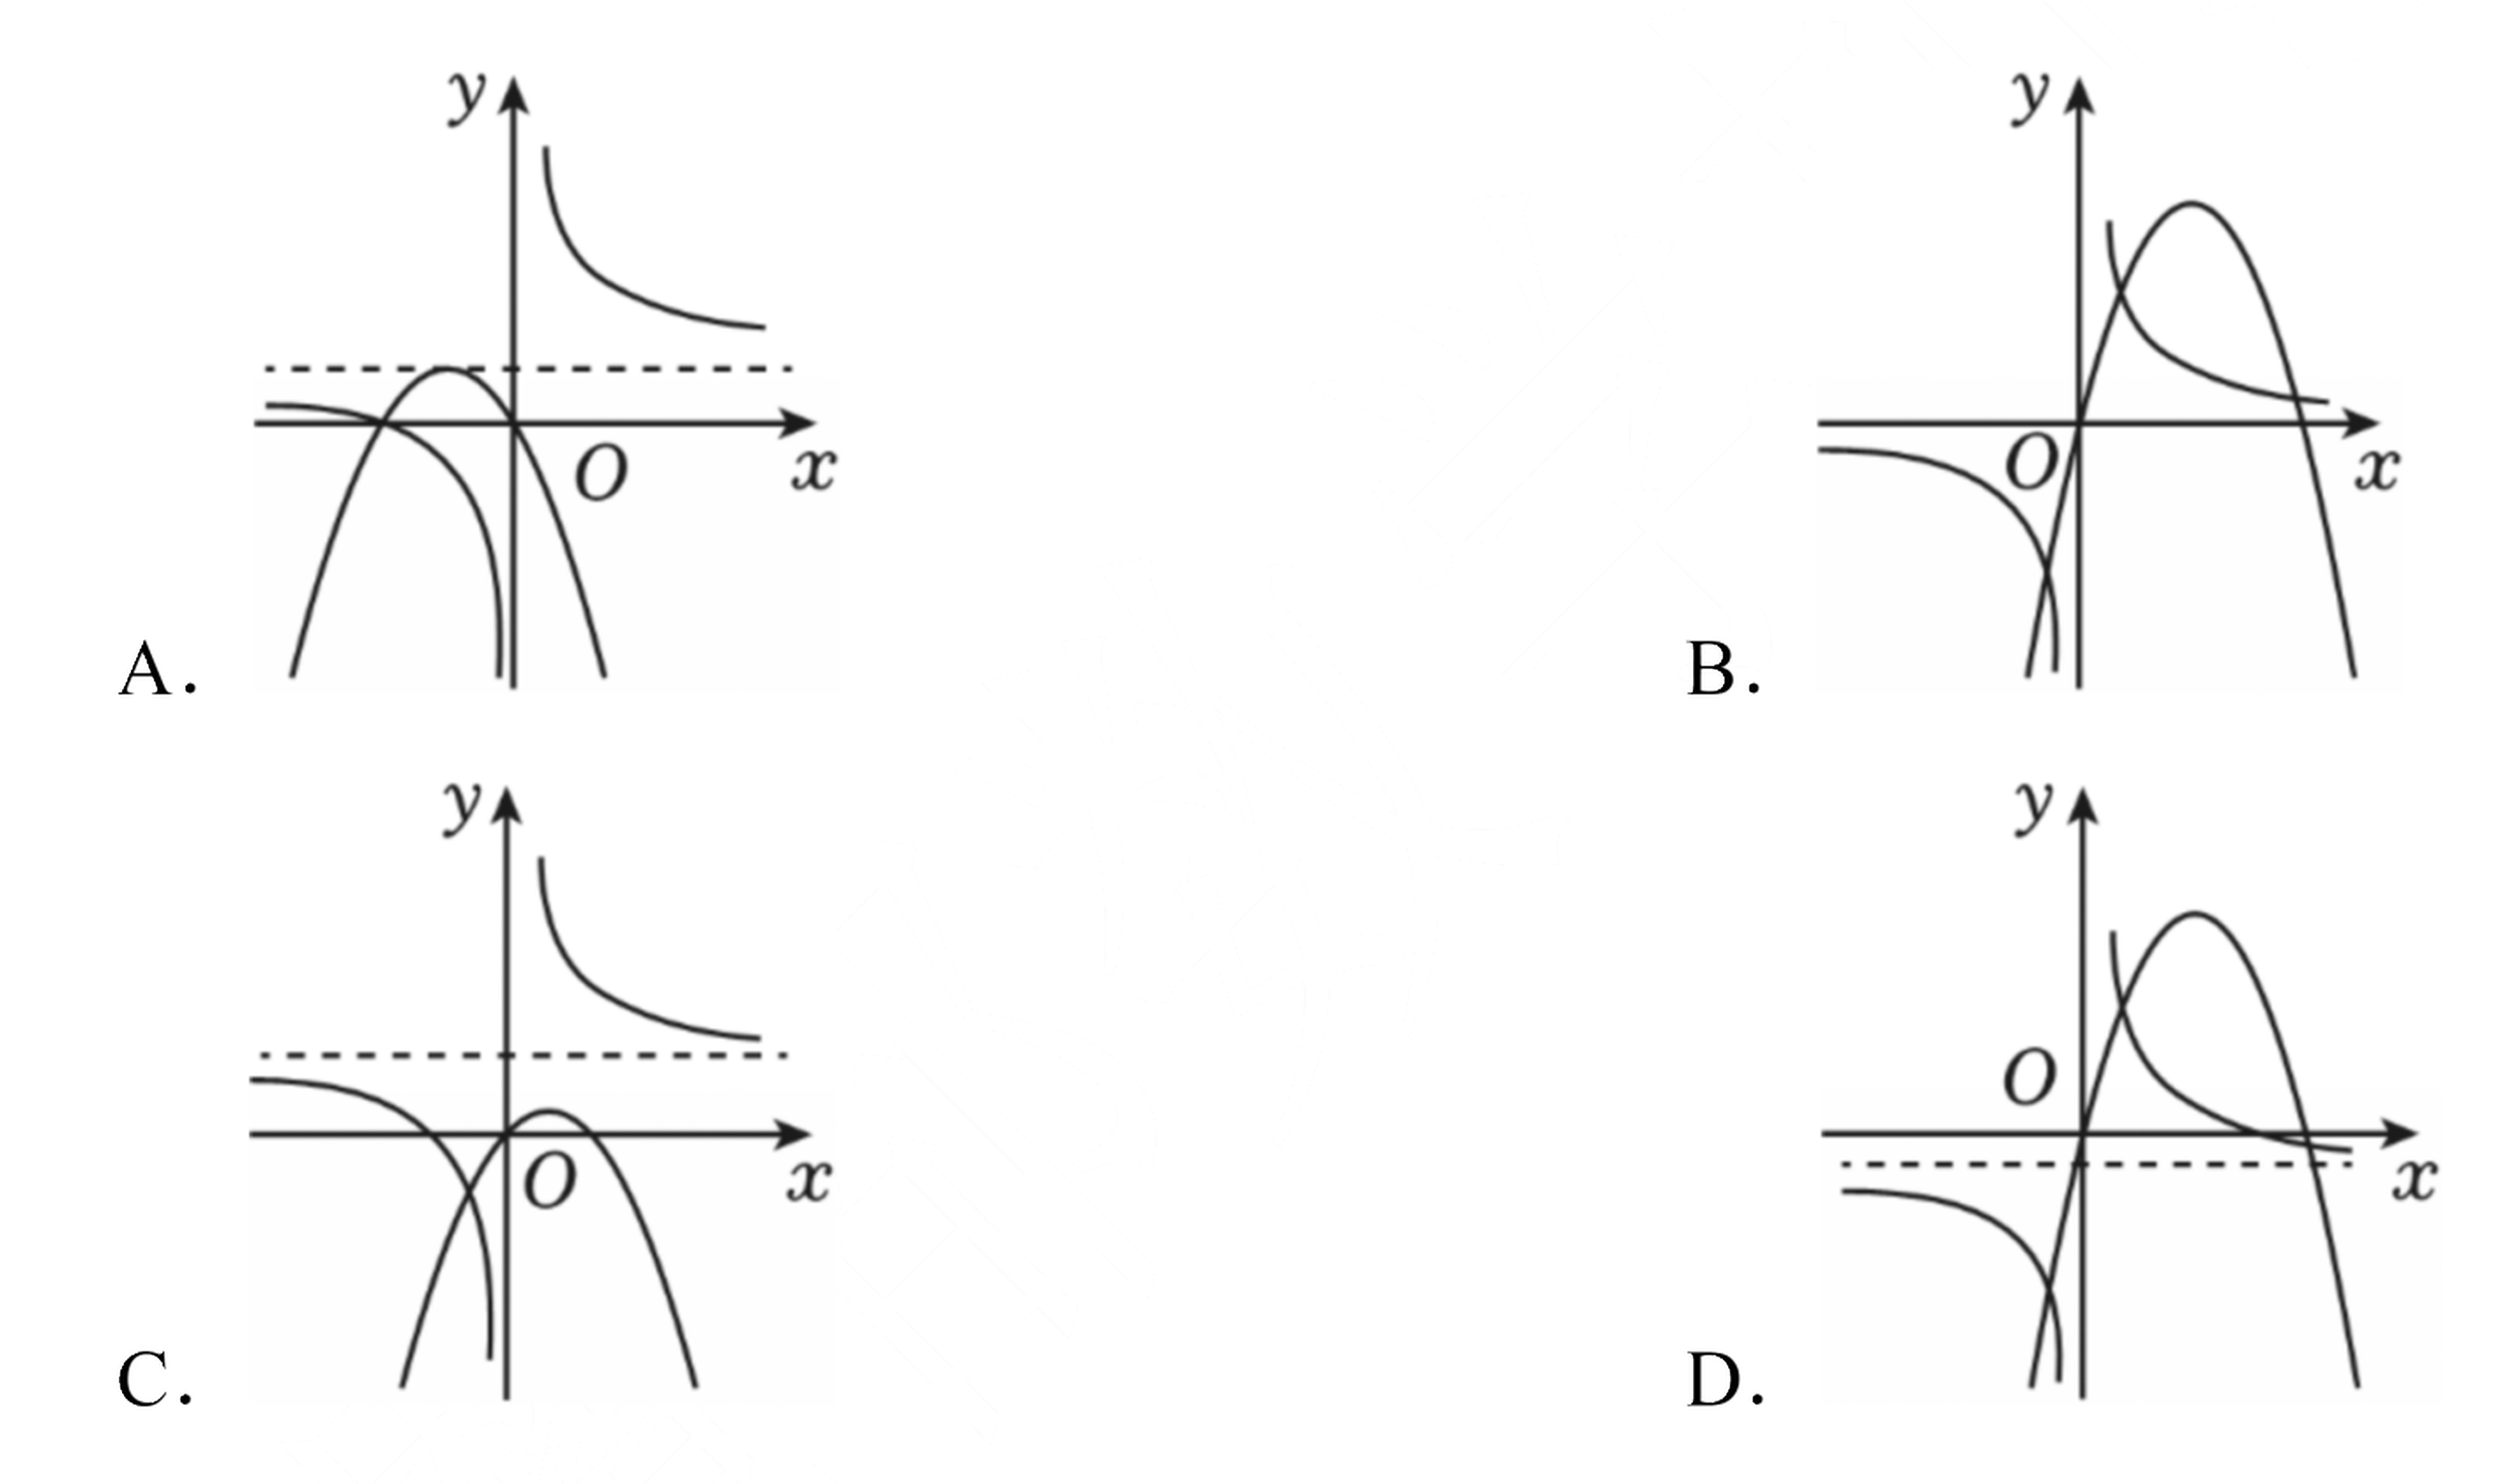
\includegraphics[width=0.80\textwidth]{figures/gao161_q14.png}
\end{center}

\ifanswer
\solbegin
\step{$A$ 选项，由二次函数图象得 $a<0$，$b<0$，由幂函数型函数图象得 $a<0$，$b>0$，}
\step{故 $A$ 选项错误；}
\step{$B$ 选项，由二次函数图象得 $a<0$，$b>0$，由幂函数型函数图象得 $a<0$，$b=0$，}
\step{故 $B$ 选项错误；}
\step{$C$ 选项，由二次函数图象得 $a<0$，$b>0$，由幂函数型函数图象得 $a<0$，$b>0$，}
\step{故 $C$ 选项正确；}
\step{$D$ 选项，由二次函数图象得 $a<0$，$b>0$，由幂函数型函数图象得 $a<0$，$b<0$，}
\step{故 $D$ 选项错误.}
\step{故选 $C$.}
\solend
\fi

% === Q15 === \subseteq／\subset、\varnothing、\mid；"排除 C""排除 B、D"正体字母照录；解析 4 行，故选 $A$
\item 设不等式 $\lvert f(x)\rvert+\lvert g(x)\rvert<a$（常数 $a>0$）的解集是 $M$，设不等式 $\lvert f(x)+g(x)\rvert<a$（常数 $a>0$）的解集是 $N$，则\mbox{（\quad）}

\keepwithprev
A. $M\subseteq N$\qquad B. $N\subseteq M$\qquad C. $M\subset N$\qquad D. $N\subset M$

\ifanswer
\solbegin
\step{$x\in M\Rightarrow\lvert f(x)+g(x)\rvert\leqslant\lvert f(x)\rvert+\lvert g(x)\rvert<a\Rightarrow x\in N$，所以 $M\subseteq N$.}
\step{取 $f(x)=g(x)=0$，则 $M=N$，排除 C.}
\step{取 $f(x)=1$，$g(x)=-1$，$a=1$，则 $M=\varnothing$，$N$ 为全体实数，排除 B、D.}
\step{故选 $A$.}
\solend
\fi

% === Q16 === "人文集"定义证明；cases 无；解析 21 行，故选 $B$
\item 设集合 $I_n=\{1,2,\cdots,n\}$，$n\in\N,n\geqslant1$，集合 $P_n=\left\{\dfrac{m}{\sqrt k}\mid m\in I_n,k\in I_n\right\}$，若 $P_n$ 的子集 $A$ 中任意两个元素之和不是整数的平方，则称 $A$ 为 “人文集”. 那么使 $P_n$ 能分成两个交集为空集的 “人文集” 的并集，且这两个人文集的并集恰为 $P_n$ 时，$n$ 的最大值是\mbox{（\quad）}

\keepwithprev
A. 13\qquad B. 14\qquad C. 15\qquad D. 16

\ifanswer
\solbegin
\step{先证当 $n\geqslant15$ 时，$P_n$ 不能分成两个不相交的人文集的并集.}
\step{假设当 $n\geqslant15$ 时，$P_n$ 可以分成两个不相交的人文集的并集，}
\step{设 $A$ 和 $B$ 为两个不相交的人文集，使 $A\cup B=P_n\supseteq I_n$.}
\step{不妨设 $1\in A$，则由于 $1+3=2^2$，所以 $3\notin A$，即 $3\in B$.}
\step{同理可得，$6\in A$，$10\in B$. 又推出 $15\in A$，}
\step{但 $1+15=4^2$，这与 $A$ 为人文集相矛盾.}
\step{再证 $P_{14}$ 满足要求. 当 $k=1$ 时，$P_{14}=\left\{\dfrac{m}{\sqrt k}\mid m\in I_{14},k\in I_{14}\right\}$，}
\step{可以分成 2 个人文集的并集.}
\step{事实上，只要取 $A_1=\{1,2,4,6,9,11,13\}$，$B_1=\{3,5,7,8,10,12,14\}$，}
\step{则 $A_1$ 和 $B_1$ 都是人文集，且 $A_1\cup B_1=P_{14}$.}
\step{当 $k=4$ 时，集合 $\left\{\dfrac{m}{\sqrt k}\mid m\in I_{14}\right\}$ 中，除整数外，}
\step{剩下的数组成集合 $\left\{\dfrac12,\dfrac32,\dfrac52,\cdots,\dfrac{13}{2}\right\}$，}
\step{可以分为下列 2 个人文集的并：$A_2=\left\{\dfrac12,\dfrac52,\dfrac92,\dfrac{11}{2}\right\}$，$B_2=\left\{\dfrac32,\dfrac72,\dfrac{13}{2}\right\}$.}
\step{当 $k=9$ 时，集合 $\left\{\dfrac{m}{\sqrt k}\mid m\in I_{14}\right\}$ 中，除整数外，}
\step{剩下的数组成集合 $\left\{\dfrac13,\dfrac23,\dfrac43,\dfrac53,\cdots,\dfrac{13}{3},\dfrac{14}{3}\right\}$，}
\step{可以分为下列 2 个人文集的并：$A_3=\left\{\dfrac13,\dfrac43,\dfrac53,\dfrac{10}{3},\dfrac{13}{3}\right\}$，$B_3=\left\{\dfrac23,\dfrac73,\dfrac83,\dfrac{11}{3},\dfrac{14}{3}\right\}$.}
\step{最后，集合 $C=\left\{\dfrac{m}{\sqrt k}\mid m\in I_{14},k\in I_{14},k\ne1,4,9\right\}$ 中的数的分母都是无理数，}
\step{它与 $P_n$ 中的任何其他数之和都不是整数，}
\step{因此，令 $A=A_1\cup A_2\cup A_3\cup C$，$B=B_1\cup B_2\cup B_3$，}
\step{则 $A$ 和 $B$ 是不相交的人文集，且 $A\cup B=P_{14}$.}
\step{综上，$n$ 的最大值为 14，故选 $B$.}
\solend
\fi

\end{enumerate}

\bigsec{三、解答题}

\begin{enumerate}
\setcounter{enumi}{16}

% === Q17 === "图像"照录；\Z；cases 块；解析 9 行，跨 06—07 页
\item (1) 已知函数 $y=x^{\frac{4m-m^2}{2}}$（$m\in\Z$）在区间 $(0,+\infty)$ 上是严格增函数，它的图像关于 $y$ 轴对称，求 $m$ 的值及该函数的解析式；

(2) 若 $(a-2)^{\frac32}<(1+2a)^{\frac32}$，求实数 $a$ 的取值范围.

\ifanswer
\solbegin
\step{(1) 由幂函数在 $(0,+\infty)$ 上严格递增，得 $\dfrac{4m-m^2}{2}>0\Leftrightarrow0<m<4$，}
\step{又 $m\in\Z$，所以 $m\in\{1,2,3\}$.}
\step{当 $m=1$ 或 $m=3$ 时，函数为 $y=x^{\frac32}$，定义域为 $[0,+\infty)$，}
\step{图像不关于 $y$ 轴对称.}
\step{当 $m=2$ 时，函数为 $y=x^2$，满足题意，所以 $m=2$，解析式 $y=x^2$.}
\step{(2) 原不等式有意义，须满足 $\begin{cases}a-2\geqslant0\\1+2a\geqslant0\end{cases}\Leftrightarrow a\geqslant2$，}
\step{函数 $y=x^{\frac32}$ 在 $[0,+\infty)$ 上严格递增，}
\step{因此 $(a-2)^{\frac32}<(1+2a)^{\frac32}\Leftrightarrow a-2<1+2a\Leftrightarrow a>-3$，}
\step{结合 $a\geqslant2$，得 $a\in[2,+\infty)$.}
\solend
\fi

% === Q18 === 题干"$a\geqslant0$"与解析"$a<0$"自相矛盾照录；"$A\cap B=(-2,-1]\cap[2,6)$"误印 ∩ 照录；\subseteq；解析 10 行
\item 已知实数 $a\geqslant0$，集合 $A=\left\{x\mid\dfrac{x+2}{x-6}<0\right\}$，$B=\{x\mid\lvert2x-1\rvert\geqslant3\}$，$C=\{x\mid x^2-3ax+2a^2<0\}$，

(1) 求 $A\cap B$；

(2) 若 $C\subseteq(A\cap B)$，求 $a$ 的取值范围.

\ifanswer
\solbegin
\step{(1) 由 $\dfrac{x+2}{x-6}<0$ 得 $-2<x<6$，即 $A=\{x\mid-2<x<6\}=(-2,6)$，}
\step{由 $\lvert2x-1\rvert\geqslant3$ 得 $2x-1\geqslant3$ 或 $2x-1\leqslant-3$，解得 $x\geqslant2$ 或 $x\leqslant-1$，}
\step{即 $B=(-\infty,-1]\cup[2,+\infty)$，}
\step{所以 $A\cap B=(-2,-1]\cap[2,6)$；}% 原卷把 ∪ 误印成 ∩，照录未改（见 ⑤ 2）
\step{(2) 由 (1) 得 $A\cap B=\{x\mid-2<x\leqslant-1\text{ 或 }2\leqslant x<6\}$，}
\step{因为 $C\subseteq(A\cap B)$，$x^2-3ax+2a^2=(x-a)(x-2a)<0$，}% 题干 $a\geqslant0$ 与解析 $a<0$ 自相矛盾，照录未改（见 ⑤ 1）
\step{当 $a=0$ 时，$C=\varnothing$，符合题意；}
\step{当 $a>0$ 时，$C=(a,2a)$，则 $\begin{cases}a\geqslant2\\2a\leqslant6\\a>0\end{cases}$，解得 $2\leqslant a\leqslant3$，}
\step{当 $a<0$ 时，$C=(2a,a)$，则 $\begin{cases}2a\geqslant-2\\a\leqslant-1\\a<0\end{cases}$，解得 $a=-1$，}
\step{故 $a$ 的范围为 $\{-1,0\}\cup[2,3]$.}
\solend
\fi

% === Q19 === 双碳太阳能应用题；"双碳""自发自用、市电互补"弯引号；解析 8 行，跨 08 页上下
\item 为响应 “双碳” 目标，某电子企业拟安装一套可使用 10 年的太阳能供电设备. 该设备的安装费用 $P(x)$（单位：万元）与太阳能电池板面积 $x(x>0)$（单位：平方米）成正比，比例系数为 $\dfrac12$. 为保障生产用电，安装后采用 “自发自用、市电互补” 模式，在此模式下，企业每年消耗的电费 $Q(x)$（单位：万元）与安装的这种太阳能电池板的面积 $x$ 之间的函数关系是 $Q(x)=\dfrac{180}{x+5}$. 记 $W(x)$（单位：万元）为该企业安装这种太阳能供电设备的费用与 10 年所消耗的电费之和.

(1) 要使该设备的安装费与第 1 年的电费之和不超过 17 万元，求安装太阳能电池板面积 $x$ 的取值范围；

(2) 当 $x$ 为多少平方米时，$W(x)$ 取得最小值？最小值是多少万元？

\ifanswer
\solbegin
\step{(1) $P(x)=\dfrac{x}{2}$，安装费与第 1 年的电费之和不超过 17 万元，即 $\dfrac{x}{2}+\dfrac{180}{x+5}\leqslant17$，}
\step{$x>0$，上式等价于 $x^2-29x+190\leqslant0\Leftrightarrow(x-10)(x-19)\leqslant0$，}
\step{解得 $x\in[10,19]$.}
\step{(2) 安装费用与 10 年电费之和为 $W(x)=P(x)+10Q(x)$，}
\step{$=\dfrac{x}{2}+\dfrac{1800}{x+5}=\dfrac{x+5}{2}+\dfrac{1800}{x+5}-\dfrac52$，}
\step{$x>0$，由基本不等式得 $W(x)\geqslant2\sqrt{\dfrac{x+5}{2}\cdot\dfrac{1800}{x+5}}-\dfrac52=60-\dfrac52=57.5$，}
\step{等号当且仅当 $\dfrac{x+5}{2}=\dfrac{1800}{x+5}$，即 $x=55$ 时成立.}
\step{因此，当电池板面积为 55 平方米时，$W(x)$ 取得最小值 57.5 万元.}
\solend
\fi

% === Q20 === $a*b$ 定义；\min 改正体；cases 块；解析 23 行，跨 08—10 页
\item 设 $a$、$b\in\R$，定义 $a*b=\begin{cases}a,&a<b\\b,&a\geqslant b\end{cases}$.

(1) 若 $x*2>1$，求 $x$ 的取值范围；

(2) 若 $(\lvert x-1\rvert+\lvert x-2\rvert)*3=3$，求 $x$ 的取值范围；

(3) 若 $a$、$b>0$，记 $M=a*\dfrac{b}{a^2+4b^2}$，分别比较 $M$ 与 $a$，以及 $M$ 与 $\dfrac{b}{a^2+4b^2}$ 的大小，并求 $M$ 的最大值.

\ifanswer
\solbegin
\step{(1) 定义 $a*b=\begin{cases}a,&a<b\\b,&a\geqslant b\end{cases}$，由 $x*2>1$，得 $\begin{cases}x<2\\x>1\end{cases}$，或 $\begin{cases}x\geqslant2\\2>1\end{cases}$，}
\step{解得 $x>1$，即 $x$ 的取值范围为 $\{x\mid x>1\}$；}
\step{(2) 当 $x\geqslant2$ 时，$\lvert x-1\rvert+\lvert x-2\rvert=2x-3\geqslant1$，}
\step{当 $1\leqslant2x-3\leqslant3$，即 $2\leqslant x\leqslant3$ 时，}
\step{此时 $(\lvert x-1\rvert+\lvert x-2\rvert)*3=2x-3=3$，解得 $x=3$；}
\step{当 $2x-3>3$，即 $x>3$ 时，}
\step{此时 $(\lvert x-1\rvert+\lvert x-2\rvert)*3=3$ 恒成立，则 $x>3$；}
\step{当 $-2x+3>3$，即 $x<0$ 时，}
\step{此时 $(\lvert x-1\rvert+\lvert x-2\rvert)*3=3$ 恒成立，则 $x<0$.}
\step{当 $1<x<2$ 时，$\lvert x-1\rvert+\lvert x-2\rvert=1$，}
\step{此时 $(\lvert x-1\rvert+\lvert x-2\rvert)*3=1\ne3$，不符合题意；}
\step{当 $x\leqslant1$ 时，$\lvert x-1\rvert+\lvert x-2\rvert=-2x+3\geqslant1$，}
\step{当 $-2x+3\leqslant3$，即 $0\leqslant x\leqslant1$ 时，}
\step{此时 $(\lvert x-1\rvert+\lvert x-2\rvert)*3=-2x+3=3$，解得 $x=0$.}
\step{综上所述，$x$ 的取值范围为 $\{x\mid x\leqslant0\text{ 或 }x\geqslant3\}$；}
\step{(3) 由题意，$M=a*\dfrac{b}{a^2+4b^2}=\min\left\{a,\dfrac{b}{a^2+4b^2}\right\}$，}% 原卷印斜体 min，按全稿惯例改正体 \min（见 ② ⑬）
\step{则 $M\leqslant a$，$M\leqslant\dfrac{b}{a^2+4b^2}$.}
\step{因为 $a$、$b>0$，所以 $\dfrac{b}{a^2+4b^2}\leqslant\dfrac{b}{2\sqrt{a^2\cdot4b^2}}=\dfrac{1}{4a}$，}
\step{当且仅当 $a=2b>0$ 时取等号，}
\step{当 $a\geqslant\dfrac{1}{4a}$，即 $a\geqslant\dfrac12$ 时，$M=a*\dfrac{b}{a^2+4b^2}=\dfrac{b}{a^2+4b^2}\leqslant\dfrac{1}{4a}$，}
\step{则 $a=\dfrac12$，$b=\dfrac14$ 时，$M$ 取得最大值 $\dfrac12$；}
\step{当 $0<a<\dfrac12$ 时，$M=a*\dfrac{b}{a^2+4b^2}=a$，此时 $M<\dfrac12$.}
\step{综上所述，$M$ 的最大值为 $\dfrac12$.}
\solend
\fi

% === Q21 === $A_n$／$B_n$／$S_n$／$T_n$ 新定义；题干第 3 问误标 (2) 照录、解析作 (3)；\prec；解析 25 行，跨 10—11 页
\item 对任意正整数 $n$，记集合 $A_n=\{(a_1,a_2,\cdots,a_n)\mid a_1,a_2,\cdots,a_n$ 均为非负整数，且 $a_1+a_2+\cdots+a_n=n\}$，集合 $B_n=\{(b_1,b_2,\cdots,b_n)\mid b_1,b_2,\cdots,b_n$ 均为非负整数，且 $b_1+b_2+\cdots+b_n=2n\}$. 设 $\alpha=(a_1,a_2,\cdots,a_n)\in A_n$，$\beta=(b_1,b_2,\cdots,b_n)\in B_n$，若对任意 $i\in\{1,2,\cdots,n\}$ 都有 $a_i\leqslant b_i$，则记 $\alpha\prec\beta$.

(1) 写出集合 $A_2$ 和 $B_2$；

(2) 证明：对任意 $\alpha\in A_n$，存在 $\beta\in B_n$，使得 $\alpha\prec\beta$；

(2) 设集合 $S_n=\{(\alpha,\beta)\mid\alpha\in A_n,\beta\in B_n,\alpha\prec\beta\}$，求证：$S_n$ 中的元素个数是完全平方数.% 原卷第 3 问题干误标 (2)（与第 2 问重号），照录未改（见 ⑤ 3）

\ifanswer
\solbegin
\step{(1) $A_2=\{(0,2),(1,1),(2,0)\}$，$B_2=\{(0,4),(1,3),(2,2),(3,1),(4,0)\}$；}
\step{(2) 对任意 $\alpha=(a_1,a_2,\cdots,a_n)\in A_n$，设 $b_i=a_i+1$（$i=1,2,3,\cdots,n$），}
\step{则 $b_1,b_2,\cdots,b_n$ 均为非负整数，且 $a_i\leqslant b_i$（$i=1,2,3,\cdots,n$）.}
\step{令 $\beta=(b_1,b_2,\cdots,b_n)$，则 $b_1+b_2+\cdots+b_n$}
\step{$=(a_1+1)+(a_2+1)+\cdots+(a_n+1)=(a_1+a_2+\cdots+a_n)+n=2n$，}
\step{所以 $\beta\in B_n$，且 $\alpha\prec\beta$.}
\step{(3) 对任意 $\alpha=(a_1,a_2,\cdots,a_n)\in A_n$，$\alpha'=(a_1',a_2',\cdots,a_n')\in A_n$，}
\step{记 $\alpha+\alpha'=(a_1+a_1',a_2+a_2',\cdots,a_n+a_n')$，}
\step{则 $a_1+a_1',a_2+a_2',\cdots,a_n+a_n'$ 均为非负整数，}
\step{且 $(a_1+a_1')+(a_2+a_2')+\cdots+(a_n+a_n')$}
\step{$=(a_1+a_2+\cdots+a_n)+(a_1'+a_2'+\cdots+a_n')=n+n=2n$，}
\step{所以 $\alpha+\alpha'\in B_n$，且 $\alpha\prec\alpha+\alpha'$，$\alpha'\prec\alpha+\alpha'$.}
\step{设集合 $A_n$ 中的元素个数为 $t$，设 $A_n=\{\alpha_1,\alpha_2,\cdots,\alpha_t\}$.}
\step{设集合 $T_n=\{(\alpha_i,\alpha_i+\alpha_j)\mid i=1,2,\cdots,t,j=1,2,\cdots,t\}$.}
\step{对任意 $\alpha_i\in A_n$（$i=1,2,\cdots,t$），都有 $\alpha_i+\alpha_1,\alpha_i+\alpha_2,\cdots,\alpha_i+\alpha_t\in B_n$，}
\step{且 $\alpha_i\prec\alpha_i+\alpha_j$，$j=1,2,\cdots,t$，所以 $T_n\subseteq S_n$.}
\step{若 $(\alpha,\beta)\in S_n$，其中 $\alpha=(a_1,a_2,\cdots,a_n)\in A_n$，$\beta=(b_1,b_2,\cdots,b_n)\in B_n$，}
\step{设 $c_i=b_i-a_i$（$i=1,2,\cdots,n$），因为 $a_i\leqslant b_i$，所以 $c_i=b_i-a_i\geqslant0$，}
\step{记 $\alpha'=(c_1,c_2,\cdots,c_n)$，}
\step{则 $c_1+c_2+\cdots+c_n=(b_1-a_1)+(b_2-a_2)+\cdots+(b_n-a_n)$}
\step{$=(b_1+b_2+\cdots+b_n)-(a_1+a_2+\cdots+a_n)=2n-n=n$，}
\step{所以 $\alpha'\in A_n$，并且有 $\beta=\alpha+\alpha'$，所以 $(\alpha,\beta)\in T_n$，所以 $S_n\subseteq T_n$，}
\step{所以 $S_n=T_n$.}
\step{因为集合 $T_n$ 中的元素个数为 $t^2$，所以 $S_n$ 中的元素个数为 $t^2$，}
\step{是完全平方数.}
\solend
\fi

\end{enumerate}

\end{document}
